\documentclass[11pt, a4paper]{article}
\usepackage[utf8]{inputenc}
\usepackage[T1]{fontenc}

\usepackage{amsmath,amssymb,amsthm,amsfonts,graphicx,float,fullpage,booktabs,bm} 
\usepackage[colorlinks,citecolor=blue,bookmarks=true]{hyperref}
\hypersetup{linkcolor=blue}
\usepackage{cleveref}
% Code listings
\usepackage{minted}
\usepackage{listings}
\usepackage{caption}
\usemintedstyle[python]{manni}
\usemintedstyle[R]{manni}
\usepackage{todonotes}
\usepackage{subcaption}
\usepackage[backend = bibtex]{biblatex}
\addbibresource{bibliography.bib}


\title{\vspace{-8ex} \huge \bfseries Stochastic Processes\\
	\LARGE \normalfont \textsc{Assignment Two} \vspace{-2ex}}
\author{\bfseries Santiago Alfonso Raposo Briceño - 100414456 \\
	\bfseries Javier Martínez Llamas - 100392684\\
	\bfseries Ricardo Hortelano Sánchez - 100418220}
\date{\vspace{-5ex}} % Remove space where date would be.

\begin{document}
	\maketitle
	\hrule

\section{Exercise 1}

The account selected for the extraction of the tweets is \textit{@realmadrid} since it has a constant number of retweets (RT), not extremely high, allowing us to measure the counting process in a reasonable time space. 
Although library \textit{rtweet} obtains information about the retweets and their time stamps it is worth mentioning that the results detailed here do not reflect the actual behaviour of the account since retweet count is limited to 100.

\subsection{Use descriptive statistics and graphics to explore the retweets data set in terms of the number of retweets by time and the time between retweets. Does it fit the hypothesis of a Poisson process?}

We know that a Poisson process is a counting process related with the Poisson and Exponential distributions. 
Being a counting process a stochastic process $\mathbf{N} = \{ N_t, t \geq 0 \}$ satisfying:
\begin{itemize}
	\item $N_t=0$
	\item $N_t$ is integer valued
	\item For $s<t, N_s \leq N_t$
	\item For $s<t, N_t - N_s$ represents the number of events that occur in the time intervals (s, t]
\end{itemize}

When plotting the tweet with maximum retweets (limited) and all the tweets we can see the behaviour of the retweet counting process.

\begin{figure}[H]
	\centering
	\begin{subfigure}{.5\textwidth}
		\centering
		% Created by tikzDevice version 0.12.3 on 2019-12-18 11:55:35
% !TEX encoding = UTF-8 Unicode
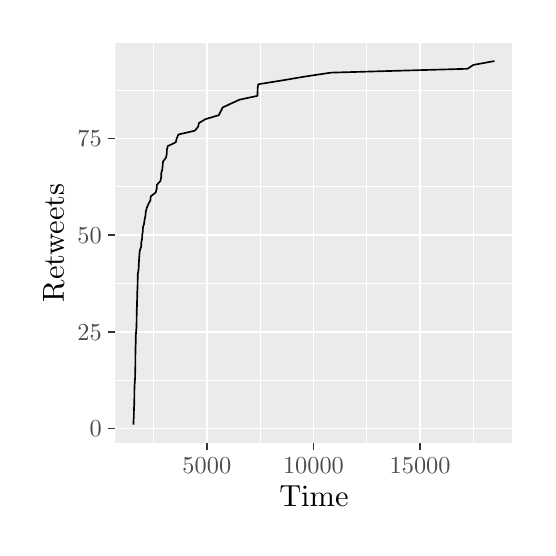
\begin{tikzpicture}[x=1pt,y=1pt]
\definecolor{fillColor}{RGB}{255,255,255}
\path[use as bounding box,fill=fillColor,fill opacity=0.00] (0,0) rectangle (180.67,180.67);
\begin{scope}
\path[clip] (  0.00,  0.00) rectangle (180.67,180.67);
\definecolor{drawColor}{RGB}{255,255,255}
\definecolor{fillColor}{RGB}{255,255,255}

\path[draw=drawColor,line width= 0.6pt,line join=round,line cap=round,fill=fillColor] (  0.00,  0.00) rectangle (180.68,180.68);
\end{scope}
\begin{scope}
\path[clip] ( 31.71, 30.69) rectangle (175.17,175.17);
\definecolor{fillColor}{gray}{0.92}

\path[fill=fillColor] ( 31.71, 30.69) rectangle (175.17,175.17);
\definecolor{drawColor}{RGB}{255,255,255}

\path[draw=drawColor,line width= 0.3pt,line join=round] ( 31.71, 53.32) --
	(175.17, 53.32);

\path[draw=drawColor,line width= 0.3pt,line join=round] ( 31.71, 88.26) --
	(175.17, 88.26);

\path[draw=drawColor,line width= 0.3pt,line join=round] ( 31.71,123.19) --
	(175.17,123.19);

\path[draw=drawColor,line width= 0.3pt,line join=round] ( 31.71,158.13) --
	(175.17,158.13);

\path[draw=drawColor,line width= 0.3pt,line join=round] ( 45.47, 30.69) --
	( 45.47,175.17);

\path[draw=drawColor,line width= 0.3pt,line join=round] ( 84.00, 30.69) --
	( 84.00,175.17);

\path[draw=drawColor,line width= 0.3pt,line join=round] (122.54, 30.69) --
	(122.54,175.17);

\path[draw=drawColor,line width= 0.3pt,line join=round] (161.07, 30.69) --
	(161.07,175.17);

\path[draw=drawColor,line width= 0.6pt,line join=round] ( 31.71, 35.86) --
	(175.17, 35.86);

\path[draw=drawColor,line width= 0.6pt,line join=round] ( 31.71, 70.79) --
	(175.17, 70.79);

\path[draw=drawColor,line width= 0.6pt,line join=round] ( 31.71,105.73) --
	(175.17,105.73);

\path[draw=drawColor,line width= 0.6pt,line join=round] ( 31.71,140.66) --
	(175.17,140.66);

\path[draw=drawColor,line width= 0.6pt,line join=round] ( 64.74, 30.69) --
	( 64.74,175.17);

\path[draw=drawColor,line width= 0.6pt,line join=round] (103.27, 30.69) --
	(103.27,175.17);

\path[draw=drawColor,line width= 0.6pt,line join=round] (141.80, 30.69) --
	(141.80,175.17);
\definecolor{drawColor}{RGB}{0,0,0}

\path[draw=drawColor,line width= 0.6pt,line join=round] ( 38.23, 37.25) --
	( 38.25, 38.65) --
	( 38.36, 40.05) --
	( 38.38, 41.45) --
	( 38.40, 42.84) --
	( 38.49, 44.24) --
	( 38.51, 45.64) --
	( 38.55, 47.04) --
	( 38.56, 48.43) --
	( 38.57, 49.83) --
	( 38.62, 51.23) --
	( 38.70, 52.62) --
	( 38.81, 54.02) --
	( 38.83, 55.42) --
	( 38.87, 56.82) --
	( 38.90, 58.21) --
	( 38.92, 59.61) --
	( 38.92, 61.01) --
	( 38.93, 62.41) --
	( 38.95, 63.80) --
	( 38.97, 65.20) --
	( 39.04, 66.60) --
	( 39.04, 68.00) --
	( 39.06, 69.39) --
	( 39.19, 70.79) --
	( 39.29, 72.19) --
	( 39.34, 73.59) --
	( 39.37, 74.98) --
	( 39.38, 76.38) --
	( 39.43, 77.78) --
	( 39.44, 79.17) --
	( 39.52, 80.57) --
	( 39.53, 81.97) --
	( 39.57, 83.37) --
	( 39.58, 84.76) --
	( 39.66, 86.16) --
	( 39.72, 87.56) --
	( 39.74, 88.96) --
	( 39.76, 90.35) --
	( 39.80, 91.75) --
	( 40.06, 93.15) --
	( 40.13, 94.55) --
	( 40.18, 95.94) --
	( 40.29, 97.34) --
	( 40.38, 98.74) --
	( 40.51,100.14) --
	( 41.01,101.53) --
	( 41.02,102.93) --
	( 41.33,104.33) --
	( 41.38,105.73) --
	( 41.63,107.12) --
	( 41.65,108.52) --
	( 42.08,109.92) --
	( 42.24,111.31) --
	( 42.56,112.71) --
	( 42.66,114.11) --
	( 43.04,115.51) --
	( 43.60,116.90) --
	( 44.36,118.30) --
	( 44.46,119.70) --
	( 46.26,121.10) --
	( 46.62,122.49) --
	( 46.71,123.89) --
	( 47.98,125.29) --
	( 48.24,126.69) --
	( 48.27,128.08) --
	( 48.65,129.48) --
	( 48.78,130.88) --
	( 48.90,132.28) --
	( 49.97,133.67) --
	( 50.25,135.07) --
	( 50.30,136.47) --
	( 50.62,137.86) --
	( 53.50,139.26) --
	( 53.86,140.66) --
	( 54.48,142.06) --
	( 60.42,143.45) --
	( 61.57,144.85) --
	( 61.92,146.25) --
	( 64.33,147.65) --
	( 69.07,149.04) --
	( 69.76,150.44) --
	( 70.46,151.84) --
	( 73.47,153.24) --
	( 76.50,154.63) --
	( 83.02,156.03) --
	( 83.07,157.43) --
	( 83.10,158.83) --
	( 83.32,160.22) --
	( 92.03,161.62) --
	(100.30,163.02) --
	(109.60,164.42) --
	(158.92,165.81) --
	(161.06,167.21) --
	(168.65,168.61);
\end{scope}
\begin{scope}
\path[clip] (  0.00,  0.00) rectangle (180.67,180.67);
\definecolor{drawColor}{gray}{0.30}

\node[text=drawColor,anchor=base east,inner sep=0pt, outer sep=0pt, scale=  0.88] at ( 26.76, 32.83) {0};

\node[text=drawColor,anchor=base east,inner sep=0pt, outer sep=0pt, scale=  0.88] at ( 26.76, 67.76) {25};

\node[text=drawColor,anchor=base east,inner sep=0pt, outer sep=0pt, scale=  0.88] at ( 26.76,102.69) {50};

\node[text=drawColor,anchor=base east,inner sep=0pt, outer sep=0pt, scale=  0.88] at ( 26.76,137.63) {75};
\end{scope}
\begin{scope}
\path[clip] (  0.00,  0.00) rectangle (180.67,180.67);
\definecolor{drawColor}{gray}{0.20}

\path[draw=drawColor,line width= 0.6pt,line join=round] ( 28.96, 35.86) --
	( 31.71, 35.86);

\path[draw=drawColor,line width= 0.6pt,line join=round] ( 28.96, 70.79) --
	( 31.71, 70.79);

\path[draw=drawColor,line width= 0.6pt,line join=round] ( 28.96,105.73) --
	( 31.71,105.73);

\path[draw=drawColor,line width= 0.6pt,line join=round] ( 28.96,140.66) --
	( 31.71,140.66);
\end{scope}
\begin{scope}
\path[clip] (  0.00,  0.00) rectangle (180.67,180.67);
\definecolor{drawColor}{gray}{0.20}

\path[draw=drawColor,line width= 0.6pt,line join=round] ( 64.74, 27.94) --
	( 64.74, 30.69);

\path[draw=drawColor,line width= 0.6pt,line join=round] (103.27, 27.94) --
	(103.27, 30.69);

\path[draw=drawColor,line width= 0.6pt,line join=round] (141.80, 27.94) --
	(141.80, 30.69);
\end{scope}
\begin{scope}
\path[clip] (  0.00,  0.00) rectangle (180.67,180.67);
\definecolor{drawColor}{gray}{0.30}

\node[text=drawColor,anchor=base,inner sep=0pt, outer sep=0pt, scale=  0.88] at ( 64.74, 19.68) {5000};

\node[text=drawColor,anchor=base,inner sep=0pt, outer sep=0pt, scale=  0.88] at (103.27, 19.68) {10000};

\node[text=drawColor,anchor=base,inner sep=0pt, outer sep=0pt, scale=  0.88] at (141.80, 19.68) {15000};
\end{scope}
\begin{scope}
\path[clip] (  0.00,  0.00) rectangle (180.67,180.67);
\definecolor{drawColor}{RGB}{0,0,0}

\node[text=drawColor,anchor=base,inner sep=0pt, outer sep=0pt, scale=  1.10] at (103.44,  7.64) {Time};
\end{scope}
\begin{scope}
\path[clip] (  0.00,  0.00) rectangle (180.67,180.67);
\definecolor{drawColor}{RGB}{0,0,0}

\node[text=drawColor,rotate= 90.00,anchor=base,inner sep=0pt, outer sep=0pt, scale=  1.10] at ( 13.08,102.93) {Retweets};
\end{scope}
\end{tikzpicture}

		\caption{Maximum RT Tweet Distribution}
		\label{fig:rtMax}
	\end{subfigure}%
	\begin{subfigure}{.5\textwidth}
		\centering
		\vspace*{-3em}
		% Created by tikzDevice version 0.12.3 on 2019-12-18 12:10:32
% !TEX encoding = UTF-8 Unicode
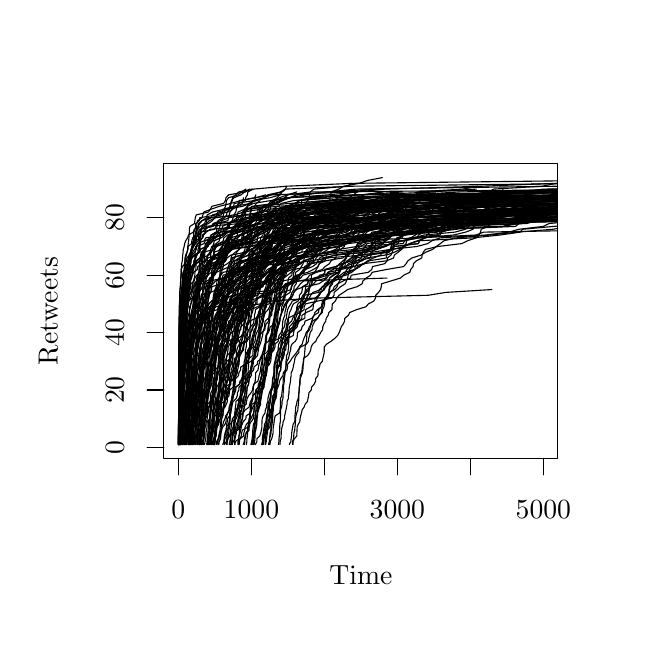
\begin{tikzpicture}[x=1pt,y=1pt]
\definecolor{fillColor}{RGB}{255,255,255}
\path[use as bounding box,fill=fillColor,fill opacity=0.00] (0,0) rectangle (216.81,216.81);
\begin{scope}
\path[clip] ( 49.20, 61.20) rectangle (191.61,167.61);
\definecolor{drawColor}{RGB}{0,0,0}

\path[draw=drawColor,line width= 0.4pt,line join=round,line cap=round] ( 84.96, 66.18) --
	( 85.16, 67.22) --
	( 85.16, 68.25) --
	( 85.66, 69.29) --
	( 86.05, 70.33) --
	( 86.29, 71.36) --
	( 86.89, 72.40) --
	( 87.11, 73.44) --
	( 87.25, 74.48) --
	( 87.54, 75.51) --
	( 87.87, 76.55) --
	( 87.99, 77.59) --
	( 88.03, 78.62) --
	( 88.16, 79.66) --
	( 88.20, 80.70) --
	( 88.41, 81.74) --
	( 88.53, 82.77) --
	( 88.65, 83.81) --
	( 89.37, 84.85) --
	( 89.47, 85.88) --
	( 89.65, 86.92) --
	( 89.81, 87.96) --
	( 89.88, 89.00) --
	( 89.94, 90.03) --
	( 89.97, 91.07) --
	( 90.00, 92.11) --
	( 90.10, 93.14) --
	( 90.60, 94.18) --
	( 91.45, 95.22) --
	( 91.54, 96.26) --
	( 92.24, 97.29) --
	( 92.53, 98.33) --
	( 92.78, 99.37) --
	( 92.78,100.40) --
	( 92.86,101.44) --
	( 92.86,102.48) --
	( 93.28,103.52) --
	( 93.61,104.55) --
	( 94.47,105.59) --
	( 94.64,106.63) --
	( 94.73,107.66) --
	( 95.89,108.70) --
	( 96.07,109.74) --
	( 97.51,110.78) --
	( 97.72,111.81) --
	( 98.24,112.85) --
	( 98.26,113.89) --
	( 98.75,114.92) --
	( 99.42,115.96) --
	( 99.51,117.00) --
	(100.39,118.03) --
	(100.69,119.07) --
	(101.38,120.11) --
	(101.54,121.15) --
	(101.75,122.18) --
	(101.99,123.22) --
	(102.70,124.26) --
	(102.76,125.29) --
	(103.64,126.33) --
	(106.88,127.37) --
	(107.34,128.41) --
	(107.45,129.44) --
	(111.26,130.48) --
	(113.58,131.52) --
	(116.96,132.55) --
	(117.85,133.59) --
	(119.81,134.63) --
	(129.39,135.67) --
	(131.34,136.70) --
	(132.54,137.74) --
	(141.20,138.78) --
	(141.53,139.81) --
	(143.34,140.85) --
	(149.07,141.89) --
	(149.45,142.93) --
	(152.65,143.96) --
	(152.76,145.00) --
	(165.64,146.04) --
	(177.92,147.07) --
	(179.89,148.11) --
	(180.27,149.15) --
	(216.81,150.12);
\end{scope}
\begin{scope}
\path[clip] (  0.00,  0.00) rectangle (216.81,216.81);
\definecolor{drawColor}{RGB}{0,0,0}

\path[draw=drawColor,line width= 0.4pt,line join=round,line cap=round] ( 54.47, 61.20) -- (186.34, 61.20);

\path[draw=drawColor,line width= 0.4pt,line join=round,line cap=round] ( 54.47, 61.20) -- ( 54.47, 55.20);

\path[draw=drawColor,line width= 0.4pt,line join=round,line cap=round] ( 80.85, 61.20) -- ( 80.85, 55.20);

\path[draw=drawColor,line width= 0.4pt,line join=round,line cap=round] (107.22, 61.20) -- (107.22, 55.20);

\path[draw=drawColor,line width= 0.4pt,line join=round,line cap=round] (133.59, 61.20) -- (133.59, 55.20);

\path[draw=drawColor,line width= 0.4pt,line join=round,line cap=round] (159.96, 61.20) -- (159.96, 55.20);

\path[draw=drawColor,line width= 0.4pt,line join=round,line cap=round] (186.34, 61.20) -- (186.34, 55.20);

\node[text=drawColor,anchor=base,inner sep=0pt, outer sep=0pt, scale=  1.00] at ( 54.47, 39.60) {0};

\node[text=drawColor,anchor=base,inner sep=0pt, outer sep=0pt, scale=  1.00] at ( 80.85, 39.60) {1000};

\node[text=drawColor,anchor=base,inner sep=0pt, outer sep=0pt, scale=  1.00] at (133.59, 39.60) {3000};

\node[text=drawColor,anchor=base,inner sep=0pt, outer sep=0pt, scale=  1.00] at (186.34, 39.60) {5000};

\path[draw=drawColor,line width= 0.4pt,line join=round,line cap=round] ( 49.20, 65.14) -- ( 49.20,148.11);

\path[draw=drawColor,line width= 0.4pt,line join=round,line cap=round] ( 49.20, 65.14) -- ( 43.20, 65.14);

\path[draw=drawColor,line width= 0.4pt,line join=round,line cap=round] ( 49.20, 85.88) -- ( 43.20, 85.88);

\path[draw=drawColor,line width= 0.4pt,line join=round,line cap=round] ( 49.20,106.63) -- ( 43.20,106.63);

\path[draw=drawColor,line width= 0.4pt,line join=round,line cap=round] ( 49.20,127.37) -- ( 43.20,127.37);

\path[draw=drawColor,line width= 0.4pt,line join=round,line cap=round] ( 49.20,148.11) -- ( 43.20,148.11);

\node[text=drawColor,rotate= 90.00,anchor=base,inner sep=0pt, outer sep=0pt, scale=  1.00] at ( 34.80, 65.14) {0};

\node[text=drawColor,rotate= 90.00,anchor=base,inner sep=0pt, outer sep=0pt, scale=  1.00] at ( 34.80, 85.88) {20};

\node[text=drawColor,rotate= 90.00,anchor=base,inner sep=0pt, outer sep=0pt, scale=  1.00] at ( 34.80,106.63) {40};

\node[text=drawColor,rotate= 90.00,anchor=base,inner sep=0pt, outer sep=0pt, scale=  1.00] at ( 34.80,127.37) {60};

\node[text=drawColor,rotate= 90.00,anchor=base,inner sep=0pt, outer sep=0pt, scale=  1.00] at ( 34.80,148.11) {80};

\path[draw=drawColor,line width= 0.4pt,line join=round,line cap=round] ( 49.20, 61.20) --
	(191.61, 61.20) --
	(191.61,167.61) --
	( 49.20,167.61) --
	( 49.20, 61.20);
\end{scope}
\begin{scope}
\path[clip] (  0.00,  0.00) rectangle (216.81,216.81);
\definecolor{drawColor}{RGB}{0,0,0}

\node[text=drawColor,anchor=base,inner sep=0pt, outer sep=0pt, scale=  1.00] at (120.41, 15.60) {Time};

\node[text=drawColor,rotate= 90.00,anchor=base,inner sep=0pt, outer sep=0pt, scale=  1.00] at ( 10.80,114.41) {Retweets};
\end{scope}
\begin{scope}
\path[clip] ( 49.20, 61.20) rectangle (191.61,167.61);
\definecolor{drawColor}{RGB}{0,0,0}

\path[draw=drawColor,line width= 0.4pt,line join=round,line cap=round] ( 54.62, 66.18) --
	( 54.62, 67.22) --
	( 54.62, 68.25) --
	( 54.63, 69.29) --
	( 54.64, 70.33) --
	( 54.64, 71.36) --
	( 54.65, 72.40) --
	( 54.66, 73.44) --
	( 54.67, 74.48) --
	( 54.68, 75.51) --
	( 54.69, 76.55) --
	( 54.69, 77.59) --
	( 54.70, 78.62) --
	( 54.70, 79.66) --
	( 54.72, 80.70) --
	( 54.74, 81.74) --
	( 54.75, 82.77) --
	( 54.75, 83.81) --
	( 54.75, 84.85) --
	( 54.76, 85.88) --
	( 54.77, 86.92) --
	( 54.79, 87.96) --
	( 54.80, 89.00) --
	( 54.87, 90.03) --
	( 54.88, 91.07) --
	( 54.89, 92.11) --
	( 54.91, 93.14) --
	( 54.92, 94.18) --
	( 54.93, 95.22) --
	( 54.99, 96.26) --
	( 54.99, 97.29) --
	( 55.04, 98.33) --
	( 55.06, 99.37) --
	( 55.07,100.40) --
	( 55.07,101.44) --
	( 55.08,102.48) --
	( 55.10,103.52) --
	( 55.13,104.55) --
	( 55.14,105.59) --
	( 55.15,106.63) --
	( 55.16,107.66) --
	( 55.19,108.70) --
	( 55.25,109.74) --
	( 55.26,110.78) --
	( 55.39,111.81) --
	( 55.42,112.85) --
	( 55.42,113.89) --
	( 55.62,114.92) --
	( 55.64,115.96) --
	( 55.78,117.00) --
	( 55.87,118.03) --
	( 55.88,119.07) --
	( 55.88,120.11) --
	( 55.97,121.15) --
	( 55.99,122.18) --
	( 55.99,123.22) --
	( 56.14,124.26) --
	( 56.17,125.29) --
	( 56.29,126.33) --
	( 56.43,127.37) --
	( 56.49,128.41) --
	( 56.59,129.44) --
	( 56.62,130.48) --
	( 56.65,131.52) --
	( 56.84,132.55) --
	( 57.10,133.59) --
	( 57.37,134.63) --
	( 57.58,135.67) --
	( 57.84,136.70) --
	( 57.86,137.74) --
	( 58.03,138.78) --
	( 58.17,139.81) --
	( 58.26,140.85) --
	( 58.33,141.89) --
	( 58.41,142.93) --
	( 58.42,143.96) --
	( 58.63,145.00) --
	( 60.29,146.04) --
	( 60.41,147.07) --
	( 60.56,148.11) --
	( 60.90,149.15) --
	( 65.31,150.19) --
	( 66.04,151.22) --
	( 66.57,152.26) --
	( 70.78,153.30) --
	( 71.46,154.33) --
	( 71.63,155.37) --
	( 72.62,156.41) --
	( 78.68,157.45) --
	( 80.15,158.48);

\path[draw=drawColor,line width= 0.4pt,line join=round,line cap=round] ( 54.84, 66.18) --
	( 54.85, 67.22) --
	( 54.85, 68.25) --
	( 54.86, 69.29) --
	( 54.86, 70.33) --
	( 54.93, 71.36) --
	( 54.94, 72.40) --
	( 54.95, 73.44) --
	( 54.95, 74.48) --
	( 54.97, 75.51) --
	( 55.01, 76.55) --
	( 55.08, 77.59) --
	( 55.11, 78.62) --
	( 55.13, 79.66) --
	( 55.17, 80.70) --
	( 55.21, 81.74) --
	( 55.23, 82.77) --
	( 55.24, 83.81) --
	( 55.34, 84.85) --
	( 55.34, 85.88) --
	( 55.36, 86.92) --
	( 55.39, 87.96) --
	( 55.44, 89.00) --
	( 55.46, 90.03) --
	( 55.46, 91.07) --
	( 55.62, 92.11) --
	( 55.71, 93.14) --
	( 55.77, 94.18) --
	( 55.83, 95.22) --
	( 55.91, 96.26) --
	( 55.99, 97.29) --
	( 56.04, 98.33) --
	( 56.08, 99.37) --
	( 56.09,100.40) --
	( 56.09,101.44) --
	( 56.09,102.48) --
	( 56.12,103.52) --
	( 56.14,104.55) --
	( 56.20,105.59) --
	( 56.25,106.63) --
	( 56.38,107.66) --
	( 56.43,108.70) --
	( 56.52,109.74) --
	( 56.54,110.78) --
	( 56.57,111.81) --
	( 56.64,112.85) --
	( 56.70,113.89) --
	( 56.74,114.92) --
	( 56.80,115.96) --
	( 56.86,117.00) --
	( 56.91,118.03) --
	( 57.06,119.07) --
	( 57.16,120.11) --
	( 57.42,121.15) --
	( 57.49,122.18) --
	( 57.57,123.22) --
	( 57.79,124.26) --
	( 57.81,125.29) --
	( 57.86,126.33) --
	( 58.06,127.37) --
	( 58.23,128.41) --
	( 58.34,129.44) --
	( 58.39,130.48) --
	( 58.47,131.52) --
	( 58.54,132.55) --
	( 58.55,133.59) --
	( 58.62,134.63) --
	( 59.11,135.67) --
	( 59.15,136.70) --
	( 59.59,137.74) --
	( 60.47,138.78) --
	( 60.62,139.81) --
	( 60.67,140.85) --
	( 60.78,141.89) --
	( 61.11,142.93) --
	( 61.22,143.96) --
	( 61.55,145.00) --
	( 62.18,146.04) --
	( 63.05,147.07) --
	( 66.24,148.11) --
	( 66.77,149.15) --
	( 70.28,150.19) --
	( 70.99,151.22) --
	( 71.50,152.26) --
	( 71.67,153.30) --
	( 71.83,154.33) --
	( 72.61,155.37) --
	( 76.10,156.41) --
	( 77.20,157.45) --
	( 78.89,158.48);

\path[draw=drawColor,line width= 0.4pt,line join=round,line cap=round] ( 54.75, 66.18) --
	( 54.76, 67.22) --
	( 54.77, 68.25) --
	( 54.77, 69.29) --
	( 54.77, 70.33) --
	( 54.79, 71.36) --
	( 54.80, 72.40) --
	( 54.80, 73.44) --
	( 54.84, 74.48) --
	( 54.84, 75.51) --
	( 54.86, 76.55) --
	( 54.88, 77.59) --
	( 54.88, 78.62) --
	( 54.91, 79.66) --
	( 54.91, 80.70) --
	( 54.94, 81.74) --
	( 54.96, 82.77) --
	( 54.98, 83.81) --
	( 54.98, 84.85) --
	( 55.00, 85.88) --
	( 55.01, 86.92) --
	( 55.02, 87.96) --
	( 55.06, 89.00) --
	( 55.08, 90.03) --
	( 55.12, 91.07) --
	( 55.14, 92.11) --
	( 55.15, 93.14) --
	( 55.16, 94.18) --
	( 55.19, 95.22) --
	( 55.21, 96.26) --
	( 55.21, 97.29) --
	( 55.22, 98.33) --
	( 55.23, 99.37) --
	( 55.33,100.40) --
	( 55.33,101.44) --
	( 55.33,102.48) --
	( 55.42,103.52) --
	( 55.57,104.55) --
	( 55.60,105.59) --
	( 56.05,106.63) --
	( 56.06,107.66) --
	( 56.17,108.70) --
	( 56.20,109.74) --
	( 56.25,110.78) --
	( 56.30,111.81) --
	( 56.31,112.85) --
	( 56.41,113.89) --
	( 56.42,114.92) --
	( 56.52,115.96) --
	( 56.56,117.00) --
	( 56.59,118.03) --
	( 56.79,119.07) --
	( 56.84,120.11) --
	( 56.99,121.15) --
	( 57.02,122.18) --
	( 57.05,123.22) --
	( 57.07,124.26) --
	( 57.28,125.29) --
	( 57.79,126.33) --
	( 58.00,127.37) --
	( 58.16,128.41) --
	( 58.21,129.44) --
	( 58.23,130.48) --
	( 58.43,131.52) --
	( 58.68,132.55) --
	( 58.76,133.59) --
	( 58.84,134.63) --
	( 59.07,135.67) --
	( 59.33,136.70) --
	( 59.81,137.74) --
	( 60.69,138.78) --
	( 60.84,139.81) --
	( 60.99,140.85) --
	( 61.33,141.89) --
	( 62.57,142.93) --
	( 62.57,143.96) --
	( 66.45,145.00) --
	( 66.99,146.04) --
	( 69.74,147.07) --
	( 71.17,148.11) --
	( 71.89,149.15) --
	( 72.05,150.19) --
	( 72.83,151.22) --
	( 73.04,152.26) --
	( 73.22,153.30) --
	( 77.07,154.33) --
	( 82.02,155.37) --
	( 82.47,156.41);

\path[draw=drawColor,line width= 0.4pt,line join=round,line cap=round] ( 54.88, 66.18) --
	( 54.89, 67.22) --
	( 54.95, 68.25) --
	( 54.95, 69.29) --
	( 54.96, 70.33) --
	( 54.97, 71.36) --
	( 54.97, 72.40) --
	( 55.00, 73.44) --
	( 55.01, 74.48) --
	( 55.05, 75.51) --
	( 55.08, 76.55) --
	( 55.10, 77.59) --
	( 55.13, 78.62) --
	( 55.15, 79.66) --
	( 55.15, 80.70) --
	( 55.17, 81.74) --
	( 55.20, 82.77) --
	( 55.21, 83.81) --
	( 55.21, 84.85) --
	( 55.26, 85.88) --
	( 55.28, 86.92) --
	( 55.28, 87.96) --
	( 55.31, 89.00) --
	( 55.34, 90.03) --
	( 55.35, 91.07) --
	( 55.35, 92.11) --
	( 55.37, 93.14) --
	( 55.37, 94.18) --
	( 55.41, 95.22) --
	( 55.44, 96.26) --
	( 55.44, 97.29) --
	( 55.59, 98.33) --
	( 55.62, 99.37) --
	( 55.63,100.40) --
	( 55.64,101.44) --
	( 55.70,102.48) --
	( 55.70,103.52) --
	( 55.70,104.55) --
	( 55.71,105.59) --
	( 55.71,106.63) --
	( 55.76,107.66) --
	( 55.77,108.70) --
	( 55.78,109.74) --
	( 55.79,110.78) --
	( 55.90,111.81) --
	( 55.90,112.85) --
	( 55.92,113.89) --
	( 55.96,114.92) --
	( 56.03,115.96) --
	( 56.08,117.00) --
	( 56.13,118.03) --
	( 56.25,119.07) --
	( 56.38,120.11) --
	( 56.49,121.15) --
	( 56.53,122.18) --
	( 57.26,123.22) --
	( 57.46,124.26) --
	( 57.48,125.29) --
	( 57.49,126.33) --
	( 57.51,127.37) --
	( 57.61,128.41) --
	( 57.76,129.44) --
	( 57.90,130.48) --
	( 57.96,131.52) --
	( 58.03,132.55) --
	( 58.21,133.59) --
	( 58.26,134.63) --
	( 58.98,135.67) --
	( 59.19,136.70) --
	( 59.51,137.74) --
	( 59.62,138.78) --
	( 59.88,139.81) --
	( 59.95,140.85) --
	( 60.00,141.89) --
	( 60.03,142.93) --
	( 60.47,143.96) --
	( 60.67,145.00) --
	( 60.71,146.04) --
	( 62.03,147.07) --
	( 62.19,148.11) --
	( 68.17,149.15) --
	( 72.32,150.19) --
	( 74.02,151.22) --
	( 74.41,152.26) --
	( 80.83,153.30);

\path[draw=drawColor,line width= 0.4pt,line join=round,line cap=round] ( 54.79, 66.18) --
	( 54.80, 67.22) --
	( 54.82, 68.25) --
	( 54.83, 69.29) --
	( 54.83, 70.33) --
	( 54.85, 71.36) --
	( 54.85, 72.40) --
	( 54.87, 73.44) --
	( 54.90, 74.48) --
	( 54.91, 75.51) --
	( 54.99, 76.55) --
	( 55.00, 77.59) --
	( 55.02, 78.62) --
	( 55.02, 79.66) --
	( 55.03, 80.70) --
	( 55.04, 81.74) --
	( 55.10, 82.77) --
	( 55.15, 83.81) --
	( 55.17, 84.85) --
	( 55.24, 85.88) --
	( 55.25, 86.92) --
	( 55.35, 87.96) --
	( 55.39, 89.00) --
	( 55.51, 90.03) --
	( 55.51, 91.07) --
	( 55.58, 92.11) --
	( 55.64, 93.14) --
	( 55.64, 94.18) --
	( 55.68, 95.22) --
	( 55.74, 96.26) --
	( 55.74, 97.29) --
	( 55.74, 98.33) --
	( 55.75, 99.37) --
	( 55.79,100.40) --
	( 55.79,101.44) --
	( 55.82,102.48) --
	( 55.92,103.52) --
	( 55.94,104.55) --
	( 55.94,105.59) --
	( 55.96,106.63) --
	( 56.07,107.66) --
	( 56.12,108.70) --
	( 56.23,109.74) --
	( 56.29,110.78) --
	( 56.36,111.81) --
	( 56.46,112.85) --
	( 56.68,113.89) --
	( 56.78,114.92) --
	( 57.28,115.96) --
	( 57.54,117.00) --
	( 57.68,118.03) --
	( 57.88,119.07) --
	( 58.26,120.11) --
	( 58.30,121.15) --
	( 58.37,122.18) --
	( 58.57,123.22) --
	( 58.78,124.26) --
	( 58.91,125.29) --
	( 59.02,126.33) --
	( 59.54,127.37) --
	( 59.65,128.41) --
	( 59.92,129.44) --
	( 59.96,130.48) --
	( 60.07,131.52) --
	( 60.48,132.55) --
	( 60.62,133.59) --
	( 61.17,134.63) --
	( 61.49,135.67) --
	( 61.53,136.70) --
	( 61.91,137.74) --
	( 62.07,138.78) --
	( 62.14,139.81) --
	( 62.23,140.85) --
	( 62.56,141.89) --
	( 62.58,142.93) --
	( 67.50,143.96) --
	( 68.03,145.00) --
	( 68.21,146.04) --
	( 72.36,147.07) --
	( 72.53,148.11) --
	( 72.84,149.15) --
	( 73.11,150.19) --
	( 74.05,151.22) --
	( 76.08,152.26) --
	( 77.55,153.30) --
	( 77.93,154.33) --
	( 77.93,155.37);

\path[draw=drawColor,line width= 0.4pt,line join=round,line cap=round] ( 55.76, 66.18) --
	( 55.76, 67.22) --
	( 55.76, 68.25) --
	( 55.78, 69.29) --
	( 55.78, 70.33) --
	( 55.78, 71.36) --
	( 55.80, 72.40) --
	( 55.83, 73.44) --
	( 55.84, 74.48) --
	( 55.85, 75.51) --
	( 55.89, 76.55) --
	( 55.94, 77.59) --
	( 55.96, 78.62) --
	( 55.97, 79.66) --
	( 55.97, 80.70) --
	( 55.98, 81.74) --
	( 55.99, 82.77) --
	( 56.01, 83.81) --
	( 56.02, 84.85) --
	( 56.03, 85.88) --
	( 56.10, 86.92) --
	( 56.12, 87.96) --
	( 56.14, 89.00) --
	( 56.17, 90.03) --
	( 56.29, 91.07) --
	( 56.52, 92.11) --
	( 56.65, 93.14) --
	( 56.79, 94.18) --
	( 56.81, 95.22) --
	( 57.04, 96.26) --
	( 57.20, 97.29) --
	( 57.25, 98.33) --
	( 57.28, 99.37) --
	( 57.29,100.40) --
	( 57.42,101.44) --
	( 57.57,102.48) --
	( 57.64,103.52) --
	( 58.05,104.55) --
	( 58.07,105.59) --
	( 58.12,106.63) --
	( 58.29,107.66) --
	( 58.32,108.70) --
	( 58.41,109.74) --
	( 58.67,110.78) --
	( 58.90,111.81) --
	( 59.24,112.85) --
	( 59.28,113.89) --
	( 59.51,114.92) --
	( 59.67,115.96) --
	( 59.76,117.00) --
	( 59.95,118.03) --
	( 59.97,119.07) --
	( 60.01,120.11) --
	( 60.02,121.15) --
	( 60.04,122.18) --
	( 60.10,123.22) --
	( 60.10,124.26) --
	( 61.10,125.29) --
	( 61.11,126.33) --
	( 61.56,127.37) --
	( 61.93,128.41) --
	( 61.94,129.44) --
	( 62.06,130.48) --
	( 62.09,131.52) --
	( 62.26,132.55) --
	( 62.59,133.59) --
	( 62.63,134.63) --
	( 63.36,135.67) --
	( 67.62,136.70) --
	( 68.23,137.74) --
	( 69.09,138.78) --
	( 72.38,139.81) --
	( 72.87,140.85) --
	( 73.14,141.89) --
	( 74.08,142.93) --
	( 75.91,143.96) --
	( 76.10,145.00) --
	( 76.84,146.04) --
	( 76.86,147.07) --
	( 80.53,148.11) --
	( 82.03,149.15);

\path[draw=drawColor,line width= 0.4pt,line join=round,line cap=round] ( 54.79, 66.18) --
	( 54.79, 67.22) --
	( 54.79, 68.25) --
	( 54.80, 69.29) --
	( 54.80, 70.33) --
	( 54.81, 71.36) --
	( 54.84, 72.40) --
	( 54.85, 73.44) --
	( 54.86, 74.48) --
	( 54.87, 75.51) --
	( 54.87, 76.55) --
	( 54.87, 77.59) --
	( 54.88, 78.62) --
	( 54.89, 79.66) --
	( 54.89, 80.70) --
	( 54.90, 81.74) --
	( 54.94, 82.77) --
	( 54.94, 83.81) --
	( 54.96, 84.85) --
	( 54.97, 85.88) --
	( 54.97, 86.92) --
	( 54.99, 87.96) --
	( 55.00, 89.00) --
	( 55.00, 90.03) --
	( 55.00, 91.07) --
	( 55.01, 92.11) --
	( 55.03, 93.14) --
	( 55.06, 94.18) --
	( 55.06, 95.22) --
	( 55.14, 96.26) --
	( 55.16, 97.29) --
	( 55.21, 98.33) --
	( 55.23, 99.37) --
	( 55.28,100.40) --
	( 55.31,101.44) --
	( 55.31,102.48) --
	( 55.37,103.52) --
	( 55.49,104.55) --
	( 55.57,105.59) --
	( 55.67,106.63) --
	( 55.75,107.66) --
	( 55.86,108.70) --
	( 55.89,109.74) --
	( 56.00,110.78) --
	( 56.14,111.81) --
	( 56.24,112.85) --
	( 56.24,113.89) --
	( 56.32,114.92) --
	( 56.45,115.96) --
	( 56.57,117.00) --
	( 56.73,118.03) --
	( 57.30,119.07) --
	( 57.72,120.11) --
	( 57.72,121.15) --
	( 58.11,122.18) --
	( 58.18,123.22) --
	( 58.29,124.26) --
	( 58.35,125.29) --
	( 58.76,126.33) --
	( 58.80,127.37) --
	( 58.86,128.41) --
	( 59.18,129.44) --
	( 59.52,130.48) --
	( 60.04,131.52) --
	( 60.14,132.55) --
	( 60.42,133.59) --
	( 60.46,134.63) --
	( 60.53,135.67) --
	( 60.58,136.70) --
	( 60.72,137.74) --
	( 61.70,138.78) --
	( 62.04,139.81) --
	( 62.40,140.85) --
	( 62.55,141.89) --
	( 62.57,142.93) --
	( 62.74,143.96) --
	( 63.07,145.00) --
	( 65.34,146.04) --
	( 66.72,147.07) --
	( 67.69,148.11) --
	( 68.54,149.15) --
	( 68.71,150.19) --
	( 72.85,151.22) --
	( 73.34,152.26) --
	( 73.38,153.30) --
	( 73.61,154.33) --
	( 74.55,155.37) --
	( 77.15,156.41) --
	( 78.40,157.45) --
	( 80.90,158.48);

\path[draw=drawColor,line width= 0.4pt,line join=round,line cap=round] ( 54.95, 66.18) --
	( 54.95, 67.22) --
	( 54.96, 68.25) --
	( 54.97, 69.29) --
	( 54.98, 70.33) --
	( 54.98, 71.36) --
	( 54.98, 72.40) --
	( 54.99, 73.44) --
	( 54.99, 74.48) --
	( 55.00, 75.51) --
	( 55.02, 76.55) --
	( 55.02, 77.59) --
	( 55.03, 78.62) --
	( 55.04, 79.66) --
	( 55.06, 80.70) --
	( 55.06, 81.74) --
	( 55.06, 82.77) --
	( 55.09, 83.81) --
	( 55.09, 84.85) --
	( 55.09, 85.88) --
	( 55.09, 86.92) --
	( 55.11, 87.96) --
	( 55.11, 89.00) --
	( 55.11, 90.03) --
	( 55.11, 91.07) --
	( 55.12, 92.11) --
	( 55.12, 93.14) --
	( 55.12, 94.18) --
	( 55.14, 95.22) --
	( 55.14, 96.26) --
	( 55.17, 97.29) --
	( 55.17, 98.33) --
	( 55.18, 99.37) --
	( 55.19,100.40) --
	( 55.21,101.44) --
	( 55.29,102.48) --
	( 55.30,103.52) --
	( 55.33,104.55) --
	( 55.34,105.59) --
	( 55.35,106.63) --
	( 55.36,107.66) --
	( 55.38,108.70) --
	( 55.40,109.74) --
	( 55.43,110.78) --
	( 55.47,111.81) --
	( 55.47,112.85) --
	( 55.53,113.89) --
	( 55.54,114.92) --
	( 55.54,115.96) --
	( 55.61,117.00) --
	( 55.69,118.03) --
	( 55.81,119.07) --
	( 55.87,120.11) --
	( 55.87,121.15) --
	( 55.96,122.18) --
	( 56.34,123.22) --
	( 56.44,124.26) --
	( 56.44,125.29) --
	( 56.82,126.33) --
	( 56.82,127.37) --
	( 56.89,128.41) --
	( 57.00,129.44) --
	( 57.16,130.48) --
	( 57.63,131.52) --
	( 57.88,132.55) --
	( 58.28,133.59) --
	( 58.76,134.63) --
	( 59.12,135.67) --
	( 59.35,136.70) --
	( 59.38,137.74) --
	( 59.99,138.78) --
	( 60.07,139.81) --
	( 60.10,140.85) --
	( 60.59,141.89) --
	( 60.62,142.93) --
	( 61.01,143.96) --
	( 61.05,145.00) --
	( 61.17,146.04) --
	( 61.42,147.07) --
	( 63.03,148.11) --
	( 63.32,149.15) --
	( 63.65,150.19) --
	( 66.30,151.22) --
	( 69.29,152.26) --
	( 73.40,153.30) --
	( 73.93,154.33) --
	( 73.95,155.37) --
	( 75.14,156.41) --
	( 76.27,157.45) --
	( 81.39,158.48);

\path[draw=drawColor,line width= 0.4pt,line join=round,line cap=round] ( 56.15, 66.18) --
	( 56.32, 67.22) --
	( 56.32, 68.25) --
	( 56.43, 69.29) --
	( 56.43, 70.33) --
	( 56.44, 71.36) --
	( 56.54, 72.40) --
	( 56.70, 73.44) --
	( 56.91, 74.48) --
	( 56.95, 75.51) --
	( 56.97, 76.55) --
	( 57.02, 77.59) --
	( 57.03, 78.62) --
	( 57.06, 79.66) --
	( 57.06, 80.70) --
	( 57.07, 81.74) --
	( 57.07, 82.77) --
	( 57.10, 83.81) --
	( 57.18, 84.85) --
	( 57.24, 85.88) --
	( 57.29, 86.92) --
	( 57.30, 87.96) --
	( 57.63, 89.00) --
	( 57.63, 90.03) --
	( 57.75, 91.07) --
	( 57.80, 92.11) --
	( 57.81, 93.14) --
	( 57.90, 94.18) --
	( 57.96, 95.22) --
	( 57.98, 96.26) --
	( 58.37, 97.29) --
	( 58.56, 98.33) --
	( 58.79, 99.37) --
	( 58.85,100.40) --
	( 58.91,101.44) --
	( 59.04,102.48) --
	( 59.04,103.52) --
	( 59.44,104.55) --
	( 59.47,105.59) --
	( 59.60,106.63) --
	( 59.61,107.66) --
	( 59.68,108.70) --
	( 59.83,109.74) --
	( 59.85,110.78) --
	( 59.89,111.81) --
	( 59.90,112.85) --
	( 60.19,113.89) --
	( 60.20,114.92) --
	( 60.56,115.96) --
	( 60.68,117.00) --
	( 61.10,118.03) --
	( 61.13,119.07) --
	( 61.26,120.11) --
	( 61.34,121.15) --
	( 61.74,122.18) --
	( 61.81,123.22) --
	( 62.47,124.26) --
	( 63.03,125.29) --
	( 63.07,126.33) --
	( 63.16,127.37) --
	( 63.22,128.41) --
	( 63.23,129.44) --
	( 63.41,130.48) --
	( 63.74,131.52) --
	( 64.42,132.55) --
	( 65.13,133.59) --
	( 68.82,134.63) --
	( 69.07,135.67) --
	( 69.38,136.70) --
	( 70.21,137.74) --
	( 70.70,138.78) --
	( 72.75,139.81) --
	( 73.47,140.85) --
	( 74.01,141.89) --
	( 74.17,142.93) --
	( 74.28,143.96) --
	( 75.22,145.00) --
	( 80.03,146.04) --
	( 80.69,147.07) --
	( 81.33,148.11) --
	( 83.18,149.15) --
	( 83.96,150.19) --
	( 84.88,151.22);

\path[draw=drawColor,line width= 0.4pt,line join=round,line cap=round] ( 57.41, 66.18) --
	( 57.45, 67.22) --
	( 57.48, 68.25) --
	( 57.49, 69.29) --
	( 57.55, 70.33) --
	( 57.56, 71.36) --
	( 57.63, 72.40) --
	( 57.72, 73.44) --
	( 57.73, 74.48) --
	( 57.73, 75.51) --
	( 57.83, 76.55) --
	( 57.89, 77.59) --
	( 57.89, 78.62) --
	( 57.94, 79.66) --
	( 57.96, 80.70) --
	( 57.97, 81.74) --
	( 57.98, 82.77) --
	( 58.03, 83.81) --
	( 58.03, 84.85) --
	( 58.05, 85.88) --
	( 58.07, 86.92) --
	( 58.37, 87.96) --
	( 58.37, 89.00) --
	( 58.46, 90.03) --
	( 58.48, 91.07) --
	( 58.55, 92.11) --
	( 58.56, 93.14) --
	( 58.59, 94.18) --
	( 58.63, 95.22) --
	( 58.71, 96.26) --
	( 58.71, 97.29) --
	( 58.76, 98.33) --
	( 58.79, 99.37) --
	( 58.84,100.40) --
	( 58.97,101.44) --
	( 59.01,102.48) --
	( 59.17,103.52) --
	( 59.19,104.55) --
	( 59.48,105.59) --
	( 59.50,106.63) --
	( 59.50,107.66) --
	( 59.51,108.70) --
	( 59.64,109.74) --
	( 59.76,110.78) --
	( 59.79,111.81) --
	( 59.93,112.85) --
	( 60.02,113.89) --
	( 60.05,114.92) --
	( 60.07,115.96) --
	( 60.15,117.00) --
	( 60.25,118.03) --
	( 60.28,119.07) --
	( 60.59,120.11) --
	( 60.69,121.15) --
	( 61.20,122.18) --
	( 61.43,123.22) --
	( 61.68,124.26) --
	( 61.91,125.29) --
	( 62.07,126.33) --
	( 62.31,127.37) --
	( 62.36,128.41) --
	( 62.56,129.44) --
	( 62.57,130.48) --
	( 62.63,131.52) --
	( 62.76,132.55) --
	( 62.77,133.59) --
	( 62.81,134.63) --
	( 62.85,135.67) --
	( 63.90,136.70) --
	( 64.04,137.74) --
	( 64.23,138.78) --
	( 65.46,139.81) --
	( 68.06,140.85) --
	( 68.31,141.89) --
	( 69.67,142.93) --
	( 69.98,143.96) --
	( 72.92,145.00) --
	( 73.21,146.04) --
	( 73.87,147.07) --
	( 74.21,148.11) --
	( 74.82,149.15) --
	( 78.00,150.19) --
	( 78.76,151.22) --
	( 81.95,152.26) --
	( 82.59,153.30) --
	( 83.98,154.33);

\path[draw=drawColor,line width= 0.4pt,line join=round,line cap=round] ( 55.12, 66.18) --
	( 55.13, 67.22) --
	( 55.14, 68.25) --
	( 55.16, 69.29) --
	( 55.18, 70.33) --
	( 55.18, 71.36) --
	( 55.21, 72.40) --
	( 55.21, 73.44) --
	( 55.21, 74.48) --
	( 55.22, 75.51) --
	( 55.23, 76.55) --
	( 55.23, 77.59) --
	( 55.25, 78.62) --
	( 55.27, 79.66) --
	( 55.31, 80.70) --
	( 55.33, 81.74) --
	( 55.37, 82.77) --
	( 55.38, 83.81) --
	( 55.38, 84.85) --
	( 55.40, 85.88) --
	( 55.41, 86.92) --
	( 55.41, 87.96) --
	( 55.44, 89.00) --
	( 55.44, 90.03) --
	( 55.46, 91.07) --
	( 55.49, 92.11) --
	( 55.57, 93.14) --
	( 55.60, 94.18) --
	( 55.62, 95.22) --
	( 55.64, 96.26) --
	( 55.64, 97.29) --
	( 55.75, 98.33) --
	( 55.84, 99.37) --
	( 55.89,100.40) --
	( 55.89,101.44) --
	( 56.03,102.48) --
	( 56.14,103.52) --
	( 56.16,104.55) --
	( 56.27,105.59) --
	( 56.35,106.63) --
	( 56.44,107.66) --
	( 56.57,108.70) --
	( 56.66,109.74) --
	( 56.66,110.78) --
	( 56.71,111.81) --
	( 56.71,112.85) --
	( 56.74,113.89) --
	( 56.78,114.92) --
	( 56.86,115.96) --
	( 56.91,117.00) --
	( 57.21,118.03) --
	( 57.39,119.07) --
	( 57.49,120.11) --
	( 57.73,121.15) --
	( 57.87,122.18) --
	( 57.91,123.22) --
	( 57.91,124.26) --
	( 58.09,125.29) --
	( 58.09,126.33) --
	( 58.40,127.37) --
	( 58.43,128.41) --
	( 58.99,129.44) --
	( 59.18,130.48) --
	( 60.05,131.52) --
	( 60.08,132.55) --
	( 60.63,133.59) --
	( 60.65,134.63) --
	( 61.93,135.67) --
	( 62.10,136.70) --
	( 62.29,137.74) --
	( 62.40,138.78) --
	( 62.45,139.81) --
	( 63.00,140.85) --
	( 63.16,141.89) --
	( 64.27,142.93) --
	( 64.40,143.96) --
	( 64.42,145.00) --
	( 64.60,146.04) --
	( 65.64,147.07) --
	( 67.92,148.11) --
	( 74.48,149.15) --
	( 75.19,150.19) --
	( 75.46,151.22) --
	( 75.48,152.26) --
	( 76.28,153.30) --
	( 76.39,154.33) --
	( 82.54,155.37) --
	( 86.03,156.41);

\path[draw=drawColor,line width= 0.4pt,line join=round,line cap=round] ( 59.15, 66.18) --
	( 59.19, 67.22) --
	( 59.20, 68.25) --
	( 59.51, 69.29) --
	( 59.55, 70.33) --
	( 59.59, 71.36) --
	( 59.61, 72.40) --
	( 59.83, 73.44) --
	( 59.86, 74.48) --
	( 60.00, 75.51) --
	( 60.08, 76.55) --
	( 60.17, 77.59) --
	( 60.21, 78.62) --
	( 60.21, 79.66) --
	( 60.29, 80.70) --
	( 60.48, 81.74) --
	( 60.56, 82.77) --
	( 60.59, 83.81) --
	( 60.73, 84.85) --
	( 60.96, 85.88) --
	( 61.34, 86.92) --
	( 61.77, 87.96) --
	( 61.82, 89.00) --
	( 62.04, 90.03) --
	( 62.16, 91.07) --
	( 62.72, 92.11) --
	( 62.77, 93.14) --
	( 62.88, 94.18) --
	( 63.15, 95.22) --
	( 63.17, 96.26) --
	( 63.21, 97.29) --
	( 63.70, 98.33) --
	( 63.87, 99.37) --
	( 64.09,100.40) --
	( 64.42,101.44) --
	( 64.58,102.48) --
	( 64.75,103.52) --
	( 65.07,104.55) --
	( 65.29,105.59) --
	( 65.51,106.63) --
	( 66.09,107.66) --
	( 66.25,108.70) --
	( 66.28,109.74) --
	( 66.38,110.78) --
	( 66.44,111.81) --
	( 66.55,112.85) --
	( 66.65,113.89) --
	( 66.74,114.92) --
	( 66.83,115.96) --
	( 67.23,117.00) --
	( 68.11,118.03) --
	( 68.30,119.07) --
	( 69.44,120.11) --
	( 69.59,121.15) --
	( 70.00,122.18) --
	( 72.01,123.22) --
	( 72.02,124.26) --
	( 72.42,125.29) --
	( 73.56,126.33) --
	( 74.58,127.37) --
	( 74.70,128.41) --
	( 75.38,129.44) --
	( 76.45,130.48) --
	( 76.72,131.52) --
	( 76.73,132.55) --
	( 77.32,133.59) --
	( 77.85,134.63) --
	( 78.15,135.67) --
	( 78.51,136.70) --
	( 78.70,137.74) --
	( 79.22,138.78) --
	( 80.23,139.81) --
	( 80.73,140.85) --
	( 80.96,141.89) --
	( 81.27,142.93) --
	( 81.33,143.96) --
	( 82.95,145.00) --
	( 83.26,146.04) --
	( 84.17,147.07) --
	( 86.48,148.11) --
	( 86.55,149.15) --
	( 86.71,150.19) --
	( 86.81,151.22) --
	( 87.21,152.26) --
	( 87.22,153.30) --
	( 87.94,154.33);

\path[draw=drawColor,line width= 0.4pt,line join=round,line cap=round] ( 60.50, 66.18) --
	( 60.50, 67.22) --
	( 60.51, 68.25) --
	( 60.73, 69.29) --
	( 60.77, 70.33) --
	( 60.87, 71.36) --
	( 61.00, 72.40) --
	( 61.09, 73.44) --
	( 61.17, 74.48) --
	( 61.45, 75.51) --
	( 61.51, 76.55) --
	( 61.59, 77.59) --
	( 61.65, 78.62) --
	( 61.95, 79.66) --
	( 62.15, 80.70) --
	( 62.17, 81.74) --
	( 62.25, 82.77) --
	( 62.27, 83.81) --
	( 62.28, 84.85) --
	( 62.31, 85.88) --
	( 62.35, 86.92) --
	( 62.38, 87.96) --
	( 62.48, 89.00) --
	( 62.51, 90.03) --
	( 62.65, 91.07) --
	( 63.11, 92.11) --
	( 63.18, 93.14) --
	( 63.22, 94.18) --
	( 63.46, 95.22) --
	( 63.49, 96.26) --
	( 63.59, 97.29) --
	( 63.91, 98.33) --
	( 63.94, 99.37) --
	( 64.08,100.40) --
	( 64.31,101.44) --
	( 64.50,102.48) --
	( 64.79,103.52) --
	( 65.26,104.55) --
	( 65.26,105.59) --
	( 65.72,106.63) --
	( 65.78,107.66) --
	( 66.02,108.70) --
	( 66.15,109.74) --
	( 66.65,110.78) --
	( 66.80,111.81) --
	( 66.91,112.85) --
	( 67.07,113.89) --
	( 67.32,114.92) --
	( 67.34,115.96) --
	( 67.41,117.00) --
	( 67.47,118.03) --
	( 67.68,119.07) --
	( 67.75,120.11) --
	( 67.80,121.15) --
	( 67.96,122.18) --
	( 68.09,123.22) --
	( 68.32,124.26) --
	( 68.40,125.29) --
	( 69.09,126.33) --
	( 69.73,127.37) --
	( 69.80,128.41) --
	( 69.87,129.44) --
	( 69.93,130.48) --
	( 70.09,131.52) --
	( 70.12,132.55) --
	( 70.50,133.59) --
	( 71.01,134.63) --
	( 72.57,135.67) --
	( 72.61,136.70) --
	( 72.70,137.74) --
	( 73.95,138.78) --
	( 75.53,139.81) --
	( 75.89,140.85) --
	( 76.96,141.89) --
	( 79.65,142.93) --
	( 80.02,143.96) --
	( 80.39,145.00) --
	( 80.70,146.04) --
	( 81.74,147.07) --
	( 81.76,148.11) --
	( 82.18,149.15) --
	( 83.72,150.19) --
	( 86.11,151.22) --
	( 86.16,152.26) --
	( 88.11,153.30) --
	( 88.72,154.33);

\path[draw=drawColor,line width= 0.4pt,line join=round,line cap=round] ( 58.46, 66.18) --
	( 58.50, 67.22) --
	( 58.55, 68.25) --
	( 58.56, 69.29) --
	( 58.63, 70.33) --
	( 58.88, 71.36) --
	( 59.06, 72.40) --
	( 59.15, 73.44) --
	( 59.26, 74.48) --
	( 59.26, 75.51) --
	( 59.35, 76.55) --
	( 59.40, 77.59) --
	( 59.44, 78.62) --
	( 59.45, 79.66) --
	( 59.56, 80.70) --
	( 59.58, 81.74) --
	( 59.67, 82.77) --
	( 59.71, 83.81) --
	( 59.74, 84.85) --
	( 59.76, 85.88) --
	( 59.86, 86.92) --
	( 59.92, 87.96) --
	( 59.93, 89.00) --
	( 59.96, 90.03) --
	( 60.00, 91.07) --
	( 60.01, 92.11) --
	( 60.08, 93.14) --
	( 60.10, 94.18) --
	( 60.18, 95.22) --
	( 60.24, 96.26) --
	( 60.44, 97.29) --
	( 60.59, 98.33) --
	( 60.59, 99.37) --
	( 60.72,100.40) --
	( 60.72,101.44) --
	( 60.82,102.48) --
	( 60.95,103.52) --
	( 61.02,104.55) --
	( 61.06,105.59) --
	( 61.07,106.63) --
	( 61.09,107.66) --
	( 61.15,108.70) --
	( 61.17,109.74) --
	( 61.23,110.78) --
	( 61.23,111.81) --
	( 61.25,112.85) --
	( 61.38,113.89) --
	( 61.42,114.92) --
	( 61.61,115.96) --
	( 61.69,117.00) --
	( 61.92,118.03) --
	( 62.06,119.07) --
	( 62.07,120.11) --
	( 62.14,121.15) --
	( 62.30,122.18) --
	( 62.31,123.22) --
	( 62.46,124.26) --
	( 62.74,125.29) --
	( 62.74,126.33) --
	( 62.84,127.37) --
	( 62.97,128.41) --
	( 63.00,129.44) --
	( 63.04,130.48) --
	( 63.10,131.52) --
	( 63.17,132.55) --
	( 63.44,133.59) --
	( 63.47,134.63) --
	( 63.67,135.67) --
	( 64.38,136.70) --
	( 64.64,137.74) --
	( 66.10,138.78) --
	( 66.94,139.81) --
	( 67.01,140.85) --
	( 67.20,141.89) --
	( 68.25,142.93) --
	( 68.32,143.96) --
	( 68.41,145.00) --
	( 68.60,146.04) --
	( 68.76,147.07) --
	( 70.55,148.11) --
	( 70.70,149.15) --
	( 70.92,150.19) --
	( 71.97,151.22) --
	( 77.71,152.26) --
	( 80.30,153.30) --
	( 81.49,154.33) --
	( 85.51,155.37) --
	( 86.78,156.41) --
	( 91.47,157.45);

\path[draw=drawColor,line width= 0.4pt,line join=round,line cap=round] ( 61.97, 66.18) --
	( 62.16, 67.22) --
	( 62.35, 68.25) --
	( 62.38, 69.29) --
	( 62.41, 70.33) --
	( 62.57, 71.36) --
	( 62.58, 72.40) --
	( 62.59, 73.44) --
	( 62.63, 74.48) --
	( 62.72, 75.51) --
	( 62.73, 76.55) --
	( 62.87, 77.59) --
	( 62.87, 78.62) --
	( 62.88, 79.66) --
	( 62.94, 80.70) --
	( 63.18, 81.74) --
	( 63.22, 82.77) --
	( 63.23, 83.81) --
	( 63.25, 84.85) --
	( 63.27, 85.88) --
	( 63.34, 86.92) --
	( 63.36, 87.96) --
	( 63.43, 89.00) --
	( 63.59, 90.03) --
	( 63.59, 91.07) --
	( 63.62, 92.11) --
	( 63.67, 93.14) --
	( 63.80, 94.18) --
	( 63.91, 95.22) --
	( 63.98, 96.26) --
	( 64.28, 97.29) --
	( 64.46, 98.33) --
	( 64.47, 99.37) --
	( 64.55,100.40) --
	( 64.58,101.44) --
	( 64.61,102.48) --
	( 64.85,103.52) --
	( 64.90,104.55) --
	( 65.08,105.59) --
	( 65.09,106.63) --
	( 65.12,107.66) --
	( 65.15,108.70) --
	( 65.28,109.74) --
	( 65.42,110.78) --
	( 65.44,111.81) --
	( 65.92,112.85) --
	( 66.26,113.89) --
	( 66.87,114.92) --
	( 67.38,115.96) --
	( 67.39,117.00) --
	( 67.52,118.03) --
	( 68.14,119.07) --
	( 68.33,120.11) --
	( 68.76,121.15) --
	( 69.05,122.18) --
	( 69.20,123.22) --
	( 69.46,124.26) --
	( 69.55,125.29) --
	( 69.59,126.33) --
	( 69.69,127.37) --
	( 70.16,128.41) --
	( 70.23,129.44) --
	( 70.66,130.48) --
	( 70.71,131.52) --
	( 70.87,132.55) --
	( 71.57,133.59) --
	( 71.58,134.63) --
	( 71.98,135.67) --
	( 71.98,136.70) --
	( 72.70,137.74) --
	( 72.80,138.78) --
	( 72.84,139.81) --
	( 73.03,140.85) --
	( 73.41,141.89) --
	( 75.42,142.93) --
	( 77.76,143.96) --
	( 78.01,145.00) --
	( 78.31,146.04) --
	( 82.11,147.07) --
	( 83.06,148.11) --
	( 83.53,149.15) --
	( 83.60,150.19) --
	( 84.06,151.22) --
	( 85.49,152.26) --
	( 87.68,153.30) --
	( 88.51,154.33) --
	( 90.20,155.37) --
	( 90.99,156.41) --
	( 91.46,157.45) --
	( 93.06,158.48) --
	( 93.62,159.52);

\path[draw=drawColor,line width= 0.4pt,line join=round,line cap=round] ( 59.53, 66.18) --
	( 59.54, 67.22) --
	( 59.60, 68.25) --
	( 59.61, 69.29) --
	( 59.73, 70.33) --
	( 59.77, 71.36) --
	( 59.77, 72.40) --
	( 59.84, 73.44) --
	( 59.87, 74.48) --
	( 59.94, 75.51) --
	( 59.95, 76.55) --
	( 60.07, 77.59) --
	( 60.28, 78.62) --
	( 60.30, 79.66) --
	( 60.32, 80.70) --
	( 60.41, 81.74) --
	( 60.59, 82.77) --
	( 60.63, 83.81) --
	( 60.68, 84.85) --
	( 60.89, 85.88) --
	( 60.92, 86.92) --
	( 61.04, 87.96) --
	( 61.08, 89.00) --
	( 61.11, 90.03) --
	( 61.18, 91.07) --
	( 61.35, 92.11) --
	( 61.41, 93.14) --
	( 61.60, 94.18) --
	( 61.97, 95.22) --
	( 61.99, 96.26) --
	( 62.12, 97.29) --
	( 62.16, 98.33) --
	( 62.37, 99.37) --
	( 62.55,100.40) --
	( 62.59,101.44) --
	( 62.60,102.48) --
	( 63.02,103.52) --
	( 63.18,104.55) --
	( 63.38,105.59) --
	( 63.39,106.63) --
	( 63.88,107.66) --
	( 64.01,108.70) --
	( 64.02,109.74) --
	( 64.13,110.78) --
	( 64.41,111.81) --
	( 64.56,112.85) --
	( 64.70,113.89) --
	( 64.79,114.92) --
	( 64.87,115.96) --
	( 64.90,117.00) --
	( 65.26,118.03) --
	( 65.46,119.07) --
	( 65.67,120.11) --
	( 65.77,121.15) --
	( 65.85,122.18) --
	( 65.98,123.22) --
	( 66.54,124.26) --
	( 66.94,125.29) --
	( 66.98,126.33) --
	( 67.37,127.37) --
	( 67.60,128.41) --
	( 67.66,129.44) --
	( 67.80,130.48) --
	( 69.00,131.52) --
	( 69.09,132.55) --
	( 69.86,133.59) --
	( 71.15,134.63) --
	( 71.56,135.67) --
	( 71.69,136.70) --
	( 72.48,137.74) --
	( 72.68,138.78) --
	( 72.80,139.81) --
	( 73.23,140.85) --
	( 73.26,141.89) --
	( 73.39,142.93) --
	( 73.62,143.96) --
	( 75.16,145.00) --
	( 75.34,146.04) --
	( 75.35,147.07) --
	( 75.55,148.11) --
	( 77.56,149.15) --
	( 78.04,150.19) --
	( 84.34,151.22) --
	( 86.11,152.26);

\path[draw=drawColor,line width= 0.4pt,line join=round,line cap=round] ( 62.55, 66.18) --
	( 62.69, 67.22) --
	( 62.74, 68.25) --
	( 62.79, 69.29) --
	( 62.86, 70.33) --
	( 62.91, 71.36) --
	( 62.95, 72.40) --
	( 63.04, 73.44) --
	( 63.12, 74.48) --
	( 63.15, 75.51) --
	( 63.45, 76.55) --
	( 63.48, 77.59) --
	( 63.61, 78.62) --
	( 63.62, 79.66) --
	( 63.70, 80.70) --
	( 63.70, 81.74) --
	( 63.75, 82.77) --
	( 63.78, 83.81) --
	( 63.78, 84.85) --
	( 63.83, 85.88) --
	( 63.86, 86.92) --
	( 63.89, 87.96) --
	( 64.05, 89.00) --
	( 64.13, 90.03) --
	( 64.31, 91.07) --
	( 64.37, 92.11) --
	( 64.41, 93.14) --
	( 64.43, 94.18) --
	( 64.60, 95.22) --
	( 64.73, 96.26) --
	( 65.05, 97.29) --
	( 65.12, 98.33) --
	( 65.14, 99.37) --
	( 65.37,100.40) --
	( 65.44,101.44) --
	( 65.62,102.48) --
	( 65.72,103.52) --
	( 65.75,104.55) --
	( 65.87,105.59) --
	( 65.96,106.63) --
	( 66.10,107.66) --
	( 66.18,108.70) --
	( 66.18,109.74) --
	( 66.30,110.78) --
	( 66.38,111.81) --
	( 66.62,112.85) --
	( 66.63,113.89) --
	( 66.67,114.92) --
	( 66.78,115.96) --
	( 67.28,117.00) --
	( 67.40,118.03) --
	( 67.52,119.07) --
	( 67.59,120.11) --
	( 67.60,121.15) --
	( 67.67,122.18) --
	( 68.74,123.22) --
	( 69.11,124.26) --
	( 69.16,125.29) --
	( 69.36,126.33) --
	( 69.40,127.37) --
	( 69.51,128.41) --
	( 69.54,129.44) --
	( 69.68,130.48) --
	( 70.54,131.52) --
	( 71.50,132.55) --
	( 71.67,133.59) --
	( 72.21,134.63) --
	( 72.41,135.67) --
	( 73.29,136.70) --
	( 73.32,137.74) --
	( 73.56,138.78) --
	( 74.40,139.81) --
	( 74.97,140.85) --
	( 75.83,141.89) --
	( 75.84,142.93) --
	( 75.95,143.96) --
	( 76.64,145.00) --
	( 76.69,146.04) --
	( 77.06,147.07) --
	( 77.10,148.11) --
	( 77.29,149.15) --
	( 77.66,150.19) --
	( 78.32,151.22) --
	( 79.40,152.26) --
	( 79.74,153.30) --
	( 82.75,154.33) --
	( 85.64,155.37) --
	( 87.85,156.41) --
	( 91.83,157.45) --
	( 93.14,158.48);

\path[draw=drawColor,line width= 0.4pt,line join=round,line cap=round] ( 67.66, 66.18) --
	( 67.73, 67.22) --
	( 67.74, 68.25) --
	( 67.76, 69.29) --
	( 67.91, 70.33) --
	( 67.96, 71.36) --
	( 68.01, 72.40) --
	( 68.01, 73.44) --
	( 68.03, 74.48) --
	( 68.24, 75.51) --
	( 68.24, 76.55) --
	( 68.26, 77.59) --
	( 68.41, 78.62) --
	( 68.47, 79.66) --
	( 68.55, 80.70) --
	( 68.71, 81.74) --
	( 68.73, 82.77) --
	( 68.79, 83.81) --
	( 68.79, 84.85) --
	( 68.91, 85.88) --
	( 69.00, 86.92) --
	( 69.25, 87.96) --
	( 69.33, 89.00) --
	( 69.38, 90.03) --
	( 69.40, 91.07) --
	( 69.45, 92.11) --
	( 69.54, 93.14) --
	( 69.65, 94.18) --
	( 69.65, 95.22) --
	( 69.70, 96.26) --
	( 69.72, 97.29) --
	( 69.74, 98.33) --
	( 69.78, 99.37) --
	( 69.80,100.40) --
	( 69.96,101.44) --
	( 69.96,102.48) --
	( 70.37,103.52) --
	( 70.43,104.55) --
	( 70.62,105.59) --
	( 70.63,106.63) --
	( 70.72,107.66) --
	( 70.80,108.70) --
	( 70.89,109.74) --
	( 70.99,110.78) --
	( 71.05,111.81) --
	( 71.05,112.85) --
	( 71.13,113.89) --
	( 71.64,114.92) --
	( 71.73,115.96) --
	( 71.87,117.00) --
	( 71.94,118.03) --
	( 71.99,119.07) --
	( 72.06,120.11) --
	( 72.23,121.15) --
	( 72.28,122.18) --
	( 72.31,123.22) --
	( 72.37,124.26) --
	( 72.37,125.29) --
	( 72.45,126.33) --
	( 72.53,127.37) --
	( 72.67,128.41) --
	( 72.81,129.44) --
	( 73.31,130.48) --
	( 73.76,131.52) --
	( 74.28,132.55) --
	( 74.76,133.59) --
	( 75.18,134.63) --
	( 75.51,135.67) --
	( 76.41,136.70) --
	( 76.48,137.74) --
	( 77.35,138.78) --
	( 77.66,139.81) --
	( 78.01,140.85) --
	( 78.10,141.89) --
	( 78.27,142.93) --
	( 78.61,143.96) --
	( 78.81,145.00) --
	( 79.60,146.04) --
	( 80.17,147.07) --
	( 80.19,148.11) --
	( 80.33,149.15) --
	( 80.42,150.19) --
	( 80.44,151.22) --
	( 85.65,152.26) --
	( 87.97,153.30) --
	( 89.39,154.33) --
	( 90.97,155.37) --
	( 93.89,156.41) --
	( 97.23,157.45);

\path[draw=drawColor,line width= 0.4pt,line join=round,line cap=round] ( 65.43, 66.18) --
	( 65.81, 67.22) --
	( 66.17, 68.25) --
	( 66.50, 69.29) --
	( 66.54, 70.33) --
	( 66.75, 71.36) --
	( 67.08, 72.40) --
	( 67.30, 73.44) --
	( 67.31, 74.48) --
	( 67.38, 75.51) --
	( 67.55, 76.55) --
	( 67.58, 77.59) --
	( 67.99, 78.62) --
	( 68.91, 79.66) --
	( 69.18, 80.70) --
	( 71.30, 81.74) --
	( 71.85, 82.77) --
	( 72.72, 83.81) --
	( 72.88, 84.85) --
	( 73.01, 85.88) --
	( 74.27, 86.92) --
	( 74.30, 87.96) --
	( 74.31, 89.00) --
	( 75.06, 90.03) --
	( 75.28, 91.07) --
	( 75.78, 92.11) --
	( 75.86, 93.14) --
	( 76.10, 94.18) --
	( 76.37, 95.22) --
	( 76.45, 96.26) --
	( 76.46, 97.29) --
	( 76.74, 98.33) --
	( 77.29, 99.37) --
	( 77.97,100.40) --
	( 78.01,101.44) --
	( 78.12,102.48) --
	( 78.38,103.52) --
	( 78.47,104.55) --
	( 78.58,105.59) --
	( 78.60,106.63) --
	( 78.91,107.66) --
	( 78.94,108.70) --
	( 79.39,109.74) --
	( 79.68,110.78) --
	( 79.96,111.81) --
	( 80.13,112.85) --
	( 80.26,113.89) --
	( 80.32,114.92) --
	( 80.69,115.96) --
	( 80.85,117.00) --
	( 80.88,118.03) --
	( 81.09,119.07) --
	( 81.26,120.11) --
	( 81.26,121.15) --
	( 81.65,122.18) --
	( 82.34,123.22) --
	( 82.51,124.26) --
	( 82.71,125.29) --
	( 83.06,126.33) --
	( 83.89,127.37) --
	( 83.96,128.41) --
	( 83.98,129.44) --
	( 84.14,130.48) --
	( 84.21,131.52) --
	( 85.89,132.55) --
	( 86.11,133.59) --
	( 86.18,134.63) --
	( 86.31,135.67) --
	( 86.34,136.70) --
	( 86.77,137.74) --
	( 86.85,138.78) --
	( 86.98,139.81) --
	( 87.77,140.85) --
	( 87.86,141.89) --
	( 88.47,142.93) --
	( 88.80,143.96) --
	( 89.40,145.00) --
	( 89.64,146.04) --
	( 90.65,147.07) --
	( 91.11,148.11) --
	( 91.77,149.15) --
	( 91.94,150.19) --
	( 96.95,151.22) --
	( 97.77,152.26) --
	(101.58,153.30) --
	(110.55,154.33) --
	(112.33,155.37) --
	(112.92,156.41) --
	(117.75,157.45) --
	(124.32,158.48);

\path[draw=drawColor,line width= 0.4pt,line join=round,line cap=round] ( 90.61, 66.18) --
	( 90.80, 67.22) --
	( 90.82, 68.25) --
	( 90.93, 69.29) --
	( 91.05, 70.33) --
	( 91.06, 71.36) --
	( 91.08, 72.40) --
	( 91.12, 73.44) --
	( 91.29, 74.48) --
	( 91.33, 75.51) --
	( 91.34, 76.55) --
	( 91.34, 77.59) --
	( 91.35, 78.62) --
	( 91.73, 79.66) --
	( 91.88, 80.70) --
	( 91.89, 81.74) --
	( 92.23, 82.77) --
	( 92.29, 83.81) --
	( 92.32, 84.85) --
	( 92.42, 85.88) --
	( 92.46, 86.92) --
	( 92.53, 87.96) --
	( 92.73, 89.00) --
	( 92.75, 90.03) --
	( 92.91, 91.07) --
	( 93.04, 92.11) --
	( 93.25, 93.14) --
	( 93.28, 94.18) --
	( 93.31, 95.22) --
	( 93.35, 96.26) --
	( 93.51, 97.29) --
	( 93.54, 98.33) --
	( 94.05, 99.37) --
	( 94.15,100.40) --
	( 94.29,101.44) --
	( 94.30,102.48) --
	( 94.34,103.52) --
	( 94.37,104.55) --
	( 94.58,105.59) --
	( 94.67,106.63) --
	( 95.71,107.66) --
	( 96.46,108.70) --
	( 96.63,109.74) --
	( 96.69,110.78) --
	( 96.82,111.81) --
	( 97.23,112.85) --
	( 97.67,113.89) --
	( 97.74,114.92) --
	( 98.29,115.96) --
	( 98.62,117.00) --
	( 98.72,118.03) --
	( 99.63,119.07) --
	( 99.82,120.11) --
	(100.70,121.15) --
	(101.59,122.18) --
	(101.70,123.22) --
	(101.93,124.26) --
	(102.11,125.29) --
	(102.50,126.33) --
	(102.51,127.37) --
	(103.72,128.41) --
	(104.32,129.44) --
	(104.88,130.48) --
	(105.41,131.52) --
	(106.23,132.55) --
	(107.80,133.59) --
	(107.90,134.63) --
	(108.76,135.67) --
	(111.26,136.70) --
	(112.66,137.74) --
	(115.15,138.78) --
	(115.50,139.81) --
	(117.08,140.85) --
	(117.95,141.89) --
	(118.07,142.93) --
	(120.77,143.96) --
	(121.00,145.00) --
	(121.94,146.04) --
	(122.34,147.07) --
	(122.76,148.11) --
	(123.06,149.15) --
	(123.86,150.19) --
	(127.94,151.22) --
	(128.05,152.26) --
	(129.14,153.30);

\path[draw=drawColor,line width= 0.4pt,line join=round,line cap=round] ( 72.80, 66.18) --
	( 73.04, 67.22) --
	( 73.36, 68.25) --
	( 73.44, 69.29) --
	( 73.80, 70.33) --
	( 75.06, 71.36) --
	( 75.16, 72.40) --
	( 75.37, 73.44) --
	( 75.87, 74.48) --
	( 76.06, 75.51) --
	( 76.44, 76.55) --
	( 76.69, 77.59) --
	( 77.27, 78.62) --
	( 77.34, 79.66) --
	( 77.39, 80.70) --
	( 77.68, 81.74) --
	( 77.77, 82.77) --
	( 78.27, 83.81) --
	( 78.49, 84.85) --
	( 78.53, 85.88) --
	( 78.56, 86.92) --
	( 78.76, 87.96) --
	( 78.82, 89.00) --
	( 79.10, 90.03) --
	( 79.64, 91.07) --
	( 80.60, 92.11) --
	( 80.61, 93.14) --
	( 80.76, 94.18) --
	( 81.20, 95.22) --
	( 81.36, 96.26) --
	( 81.42, 97.29) --
	( 82.05, 98.33) --
	( 82.18, 99.37) --
	( 82.24,100.40) --
	( 82.29,101.44) --
	( 82.44,102.48) --
	( 82.71,103.52) --
	( 83.05,104.55) --
	( 83.33,105.59) --
	( 83.50,106.63) --
	( 83.75,107.66) --
	( 83.76,108.70) --
	( 83.89,109.74) --
	( 84.20,110.78) --
	( 84.51,111.81) --
	( 84.65,112.85) --
	( 84.84,113.89) --
	( 84.94,114.92) --
	( 85.08,115.96) --
	( 85.15,117.00) --
	( 85.25,118.03) --
	( 85.54,119.07) --
	( 86.24,120.11) --
	( 86.28,121.15) --
	( 86.82,122.18) --
	( 87.53,123.22) --
	( 88.28,124.26) --
	( 88.88,125.29) --
	( 88.92,126.33) --
	( 89.42,127.37) --
	( 89.49,128.41) --
	( 89.59,129.44) --
	( 89.68,130.48) --
	( 89.87,131.52) --
	( 90.93,132.55) --
	( 90.94,133.59) --
	( 91.06,134.63) --
	( 91.26,135.67) --
	( 91.44,136.70) --
	( 91.53,137.74) --
	( 91.61,138.78) --
	( 91.76,139.81) --
	( 91.79,140.85) --
	( 91.80,141.89) --
	( 91.88,142.93) --
	( 91.96,143.96) --
	( 92.23,145.00) --
	( 92.31,146.04) --
	( 93.42,147.07) --
	( 93.56,148.11) --
	( 94.13,149.15) --
	( 94.35,150.19) --
	( 94.39,151.22) --
	( 94.68,152.26) --
	( 96.44,153.30) --
	( 98.35,154.33) --
	(101.79,155.37) --
	(101.80,156.41) --
	(102.09,157.45) --
	(103.46,158.48) --
	(115.51,159.52) --
	(117.08,160.56);

\path[draw=drawColor,line width= 0.4pt,line join=round,line cap=round] ( 64.98, 66.18) --
	( 65.01, 67.22) --
	( 65.03, 68.25) --
	( 65.05, 69.29) --
	( 65.10, 70.33) --
	( 65.19, 71.36) --
	( 65.32, 72.40) --
	( 65.32, 73.44) --
	( 65.35, 74.48) --
	( 65.93, 75.51) --
	( 66.06, 76.55) --
	( 66.10, 77.59) --
	( 66.11, 78.62) --
	( 66.27, 79.66) --
	( 66.33, 80.70) --
	( 66.49, 81.74) --
	( 67.19, 82.77) --
	( 67.41, 83.81) --
	( 67.58, 84.85) --
	( 67.75, 85.88) --
	( 67.98, 86.92) --
	( 68.13, 87.96) --
	( 68.21, 89.00) --
	( 68.50, 90.03) --
	( 68.52, 91.07) --
	( 68.54, 92.11) --
	( 68.55, 93.14) --
	( 68.74, 94.18) --
	( 68.95, 95.22) --
	( 68.95, 96.26) --
	( 69.24, 97.29) --
	( 69.39, 98.33) --
	( 69.59, 99.37) --
	( 69.78,100.40) --
	( 69.83,101.44) --
	( 70.21,102.48) --
	( 70.28,103.52) --
	( 70.40,104.55) --
	( 70.54,105.59) --
	( 70.94,106.63) --
	( 71.07,107.66) --
	( 71.22,108.70) --
	( 71.45,109.74) --
	( 71.50,110.78) --
	( 71.71,111.81) --
	( 72.43,112.85) --
	( 72.46,113.89) --
	( 72.81,114.92) --
	( 73.09,115.96) --
	( 73.58,117.00) --
	( 73.96,118.03) --
	( 75.02,119.07) --
	( 76.78,120.11) --
	( 77.58,121.15) --
	( 78.57,122.18) --
	( 78.96,123.22) --
	( 80.42,124.26) --
	( 81.01,125.29) --
	( 81.33,126.33) --
	( 84.29,127.37) --
	( 84.39,128.41) --
	( 84.90,129.44) --
	( 84.91,130.48) --
	( 84.94,131.52) --
	( 85.28,132.55) --
	( 85.40,133.59) --
	( 86.01,134.63) --
	( 86.73,135.67) --
	( 87.42,136.70) --
	( 90.33,137.74) --
	( 90.46,138.78) --
	( 90.67,139.81) --
	( 91.04,140.85) --
	( 92.08,141.89) --
	( 92.11,142.93) --
	( 92.52,143.96) --
	( 92.66,145.00) --
	( 93.04,146.04) --
	( 93.23,147.07) --
	( 95.14,148.11) --
	( 95.71,149.15) --
	( 95.89,150.19) --
	( 98.03,151.22) --
	( 98.12,152.26) --
	(117.09,153.30) --
	(118.65,154.33) --
	(124.08,155.37);

\path[draw=drawColor,line width= 0.4pt,line join=round,line cap=round] ( 59.50, 66.18) --
	( 59.55, 67.22) --
	( 59.58, 68.25) --
	( 59.84, 69.29) --
	( 59.94, 70.33) --
	( 59.97, 71.36) --
	( 60.08, 72.40) --
	( 60.60, 73.44) --
	( 60.66, 74.48) --
	( 60.74, 75.51) --
	( 60.84, 76.55) --
	( 60.85, 77.59) --
	( 61.01, 78.62) --
	( 61.33, 79.66) --
	( 61.48, 80.70) --
	( 61.66, 81.74) --
	( 61.80, 82.77) --
	( 62.02, 83.81) --
	( 62.06, 84.85) --
	( 62.12, 85.88) --
	( 62.18, 86.92) --
	( 62.25, 87.96) --
	( 62.29, 89.00) --
	( 62.31, 90.03) --
	( 62.38, 91.07) --
	( 62.45, 92.11) --
	( 62.59, 93.14) --
	( 62.62, 94.18) --
	( 62.91, 95.22) --
	( 63.39, 96.26) --
	( 63.91, 97.29) --
	( 64.17, 98.33) --
	( 64.70, 99.37) --
	( 64.89,100.40) --
	( 65.22,101.44) --
	( 65.25,102.48) --
	( 65.27,103.52) --
	( 65.77,104.55) --
	( 66.54,105.59) --
	( 66.57,106.63) --
	( 67.05,107.66) --
	( 67.26,108.70) --
	( 67.38,109.74) --
	( 68.28,110.78) --
	( 68.39,111.81) --
	( 68.42,112.85) --
	( 68.54,113.89) --
	( 69.18,114.92) --
	( 69.73,115.96) --
	( 69.92,117.00) --
	( 70.50,118.03) --
	( 70.61,119.07) --
	( 70.85,120.11) --
	( 70.87,121.15) --
	( 71.15,122.18) --
	( 71.82,123.22) --
	( 72.10,124.26) --
	( 72.60,125.29) --
	( 72.72,126.33) --
	( 73.54,127.37) --
	( 73.86,128.41) --
	( 74.03,129.44) --
	( 74.30,130.48) --
	( 74.79,131.52) --
	( 79.38,132.55) --
	( 79.65,133.59) --
	( 81.24,134.63) --
	( 82.08,135.67) --
	( 82.19,136.70) --
	( 83.36,137.74) --
	( 83.50,138.78) --
	( 84.47,139.81) --
	( 86.60,140.85) --
	( 87.23,141.89) --
	( 89.07,142.93) --
	( 89.51,143.96) --
	( 89.96,145.00) --
	( 90.12,146.04) --
	( 90.36,147.07) --
	( 92.78,148.11) --
	( 94.83,149.15) --
	( 95.57,150.19) --
	( 98.03,151.22) --
	( 99.73,152.26) --
	(100.35,153.30) --
	(101.16,154.33) --
	(101.94,155.37) --
	(120.96,156.41) --
	(128.47,157.45);

\path[draw=drawColor,line width= 0.4pt,line join=round,line cap=round] ( 58.64, 66.18) --
	( 59.02, 67.22) --
	( 59.46, 68.25) --
	( 59.52, 69.29) --
	( 59.89, 70.33) --
	( 59.92, 71.36) --
	( 59.94, 72.40) --
	( 60.11, 73.44) --
	( 60.39, 74.48) --
	( 60.61, 75.51) --
	( 60.85, 76.55) --
	( 60.90, 77.59) --
	( 61.41, 78.62) --
	( 61.45, 79.66) --
	( 61.52, 80.70) --
	( 61.52, 81.74) --
	( 61.75, 82.77) --
	( 62.08, 83.81) --
	( 62.11, 84.85) --
	( 62.18, 85.88) --
	( 62.45, 86.92) --
	( 62.77, 87.96) --
	( 62.85, 89.00) --
	( 62.92, 90.03) --
	( 63.03, 91.07) --
	( 63.04, 92.11) --
	( 63.25, 93.14) --
	( 63.47, 94.18) --
	( 63.50, 95.22) --
	( 63.75, 96.26) --
	( 64.07, 97.29) --
	( 64.09, 98.33) --
	( 65.10, 99.37) --
	( 65.36,100.40) --
	( 66.16,101.44) --
	( 66.34,102.48) --
	( 66.41,103.52) --
	( 66.64,104.55) --
	( 67.22,105.59) --
	( 67.42,106.63) --
	( 67.60,107.66) --
	( 67.99,108.70) --
	( 68.26,109.74) --
	( 68.60,110.78) --
	( 68.80,111.81) --
	( 68.80,112.85) --
	( 68.91,113.89) --
	( 69.28,114.92) --
	( 69.87,115.96) --
	( 69.89,117.00) --
	( 70.11,118.03) --
	( 70.63,119.07) --
	( 71.18,120.11) --
	( 71.44,121.15) --
	( 72.32,122.18) --
	( 72.52,123.22) --
	( 73.54,124.26) --
	( 74.05,125.29) --
	( 74.17,126.33) --
	( 74.49,127.37) --
	( 75.47,128.41) --
	( 76.62,129.44) --
	( 78.78,130.48) --
	( 79.14,131.52) --
	( 81.10,132.55) --
	( 81.13,133.59) --
	( 81.30,134.63) --
	( 84.84,135.67) --
	( 88.68,136.70) --
	( 90.52,137.74) --
	( 91.42,138.78) --
	( 91.93,139.81) --
	( 94.22,140.85) --
	( 96.28,141.89) --
	( 97.21,142.93) --
	( 98.92,143.96) --
	( 99.48,145.00) --
	(101.80,146.04) --
	(103.40,147.07) --
	(120.86,148.11) --
	(122.41,149.15);

\path[draw=drawColor,line width= 0.4pt,line join=round,line cap=round] ( 57.28, 66.18) --
	( 57.35, 67.22) --
	( 57.36, 68.25) --
	( 57.40, 69.29) --
	( 57.53, 70.33) --
	( 57.68, 71.36) --
	( 57.68, 72.40) --
	( 57.73, 73.44) --
	( 57.78, 74.48) --
	( 57.83, 75.51) --
	( 57.85, 76.55) --
	( 57.86, 77.59) --
	( 57.95, 78.62) --
	( 58.08, 79.66) --
	( 58.38, 80.70) --
	( 58.48, 81.74) --
	( 58.49, 82.77) --
	( 58.57, 83.81) --
	( 58.79, 84.85) --
	( 58.96, 85.88) --
	( 59.21, 86.92) --
	( 59.31, 87.96) --
	( 59.52, 89.00) --
	( 59.55, 90.03) --
	( 59.56, 91.07) --
	( 59.70, 92.11) --
	( 60.00, 93.14) --
	( 60.02, 94.18) --
	( 60.36, 95.22) --
	( 60.69, 96.26) --
	( 60.79, 97.29) --
	( 61.14, 98.33) --
	( 61.19, 99.37) --
	( 61.38,100.40) --
	( 61.58,101.44) --
	( 61.61,102.48) --
	( 61.95,103.52) --
	( 62.42,104.55) --
	( 62.43,105.59) --
	( 62.96,106.63) --
	( 62.97,107.66) --
	( 63.01,108.70) --
	( 63.12,109.74) --
	( 63.20,110.78) --
	( 63.24,111.81) --
	( 63.31,112.85) --
	( 63.68,113.89) --
	( 63.83,114.92) --
	( 64.16,115.96) --
	( 64.24,117.00) --
	( 64.37,118.03) --
	( 64.42,119.07) --
	( 64.66,120.11) --
	( 64.85,121.15) --
	( 64.97,122.18) --
	( 64.97,123.22) --
	( 65.22,124.26) --
	( 65.94,125.29) --
	( 66.27,126.33) --
	( 67.08,127.37) --
	( 67.26,128.41) --
	( 67.79,129.44) --
	( 68.01,130.48) --
	( 68.13,131.52) --
	( 68.35,132.55) --
	( 69.16,133.59) --
	( 69.59,134.63) --
	( 69.59,135.67) --
	( 69.80,136.70) --
	( 70.23,137.74) --
	( 72.16,138.78) --
	( 72.23,139.81) --
	( 72.48,140.85) --
	( 73.23,141.89) --
	( 73.69,142.93) --
	( 74.96,143.96) --
	( 75.08,145.00) --
	( 77.98,146.04) --
	( 79.34,147.07) --
	( 85.82,148.11) --
	( 91.44,149.15) --
	( 91.49,150.19) --
	( 95.28,151.22) --
	( 97.19,152.26) --
	(104.34,153.30) --
	(123.31,154.33) --
	(129.52,155.37);

\path[draw=drawColor,line width= 0.4pt,line join=round,line cap=round] ( 54.49, 66.18) --
	( 54.50, 67.22) --
	( 54.51, 68.25) --
	( 54.52, 69.29) --
	( 54.52, 70.33) --
	( 54.54, 71.36) --
	( 54.54, 72.40) --
	( 54.60, 73.44) --
	( 54.61, 74.48) --
	( 54.67, 75.51) --
	( 54.67, 76.55) --
	( 54.89, 77.59) --
	( 54.92, 78.62) --
	( 54.92, 79.66) --
	( 54.93, 80.70) --
	( 54.98, 81.74) --
	( 55.05, 82.77) --
	( 55.26, 83.81) --
	( 55.37, 84.85) --
	( 55.40, 85.88) --
	( 55.80, 86.92) --
	( 55.81, 87.96) --
	( 56.21, 89.00) --
	( 56.43, 90.03) --
	( 56.49, 91.07) --
	( 56.51, 92.11) --
	( 56.96, 93.14) --
	( 57.02, 94.18) --
	( 57.22, 95.22) --
	( 57.26, 96.26) --
	( 57.81, 97.29) --
	( 58.21, 98.33) --
	( 58.25, 99.37) --
	( 58.39,100.40) --
	( 58.44,101.44) --
	( 58.70,102.48) --
	( 58.95,103.52) --
	( 59.36,104.55) --
	( 60.04,105.59) --
	( 60.42,106.63) --
	( 60.87,107.66) --
	( 61.46,108.70) --
	( 61.66,109.74) --
	( 63.30,110.78) --
	( 64.54,111.81) --
	( 65.24,112.85) --
	( 65.53,113.89) --
	( 67.13,114.92) --
	( 67.95,115.96) --
	( 74.10,117.00) --
	( 75.83,118.03) --
	( 75.95,119.07) --
	( 81.27,120.11) --
	( 81.36,121.15) --
	( 89.82,122.18) --
	( 92.31,123.22) --
	( 94.03,124.26) --
	( 98.06,125.29) --
	(103.59,126.33);

\path[draw=drawColor,line width= 0.4pt,line join=round,line cap=round] ( 57.40, 66.18) --
	( 57.44, 67.22) --
	( 57.53, 68.25) --
	( 57.68, 69.29) --
	( 57.76, 70.33) --
	( 57.77, 71.36) --
	( 57.80, 72.40) --
	( 57.85, 73.44) --
	( 57.88, 74.48) --
	( 58.03, 75.51) --
	( 58.07, 76.55) --
	( 58.26, 77.59) --
	( 58.39, 78.62) --
	( 58.40, 79.66) --
	( 58.44, 80.70) --
	( 58.54, 81.74) --
	( 58.61, 82.77) --
	( 58.66, 83.81) --
	( 58.72, 84.85) --
	( 58.73, 85.88) --
	( 58.85, 86.92) --
	( 58.90, 87.96) --
	( 58.90, 89.00) --
	( 58.95, 90.03) --
	( 58.98, 91.07) --
	( 59.02, 92.11) --
	( 59.12, 93.14) --
	( 59.14, 94.18) --
	( 59.20, 95.22) --
	( 59.41, 96.26) --
	( 59.70, 97.29) --
	( 59.95, 98.33) --
	( 60.02, 99.37) --
	( 60.21,100.40) --
	( 60.61,101.44) --
	( 60.68,102.48) --
	( 61.00,103.52) --
	( 61.14,104.55) --
	( 61.14,105.59) --
	( 61.22,106.63) --
	( 61.35,107.66) --
	( 61.76,108.70) --
	( 61.97,109.74) --
	( 62.19,110.78) --
	( 62.20,111.81) --
	( 62.24,112.85) --
	( 62.48,113.89) --
	( 62.82,114.92) --
	( 63.27,115.96) --
	( 63.30,117.00) --
	( 63.57,118.03) --
	( 63.61,119.07) --
	( 63.97,120.11) --
	( 64.41,121.15) --
	( 64.90,122.18) --
	( 66.46,123.22) --
	( 66.48,124.26) --
	( 66.94,125.29) --
	( 67.00,126.33) --
	( 67.09,127.37) --
	( 67.33,128.41) --
	( 67.57,129.44) --
	( 67.93,130.48) --
	( 68.07,131.52) --
	( 68.24,132.55) --
	( 68.77,133.59) --
	( 68.93,134.63) --
	( 69.53,135.67) --
	( 70.16,136.70) --
	( 70.36,137.74) --
	( 70.40,138.78) --
	( 71.76,139.81) --
	( 72.02,140.85) --
	( 72.87,141.89) --
	( 73.58,142.93) --
	( 73.86,143.96) --
	( 74.55,145.00) --
	( 75.66,146.04) --
	( 76.50,147.07) --
	( 77.58,148.11) --
	( 78.23,149.15) --
	( 78.35,150.19) --
	( 79.91,151.22) --
	( 81.04,152.26) --
	( 89.12,153.30) --
	( 92.21,154.33) --
	( 94.71,155.37) --
	(100.46,156.41) --
	(107.81,157.45) --
	(126.57,158.48);

\path[draw=drawColor,line width= 0.4pt,line join=round,line cap=round] ( 76.13, 66.18) --
	( 76.16, 67.22) --
	( 76.26, 68.25) --
	( 76.35, 69.29) --
	( 76.52, 70.33) --
	( 76.55, 71.36) --
	( 76.57, 72.40) --
	( 76.75, 73.44) --
	( 76.76, 74.48) --
	( 76.79, 75.51) --
	( 76.88, 76.55) --
	( 76.99, 77.59) --
	( 77.26, 78.62) --
	( 77.44, 79.66) --
	( 77.86, 80.70) --
	( 77.97, 81.74) --
	( 77.98, 82.77) --
	( 78.43, 83.81) --
	( 78.55, 84.85) --
	( 78.75, 85.88) --
	( 78.82, 86.92) --
	( 78.85, 87.96) --
	( 79.30, 89.00) --
	( 79.32, 90.03) --
	( 79.60, 91.07) --
	( 79.64, 92.11) --
	( 79.66, 93.14) --
	( 79.78, 94.18) --
	( 79.79, 95.22) --
	( 79.82, 96.26) --
	( 80.06, 97.29) --
	( 80.22, 98.33) --
	( 80.36, 99.37) --
	( 80.59,100.40) --
	( 80.93,101.44) --
	( 81.16,102.48) --
	( 81.49,103.52) --
	( 81.58,104.55) --
	( 81.89,105.59) --
	( 82.03,106.63) --
	( 82.32,107.66) --
	( 82.35,108.70) --
	( 82.65,109.74) --
	( 82.78,110.78) --
	( 83.02,111.81) --
	( 83.04,112.85) --
	( 83.87,113.89) --
	( 83.97,114.92) --
	( 84.37,115.96) --
	( 84.98,117.00) --
	( 85.14,118.03) --
	( 85.68,119.07) --
	( 85.75,120.11) --
	( 86.50,121.15) --
	( 86.63,122.18) --
	( 86.82,123.22) --
	( 86.83,124.26) --
	( 87.43,125.29) --
	( 88.60,126.33) --
	( 89.25,127.37) --
	( 89.57,128.41) --
	( 90.98,129.44) --
	( 91.71,130.48) --
	( 92.26,131.52) --
	( 93.11,132.55) --
	( 93.51,133.59) --
	( 93.64,134.63) --
	( 94.06,135.67) --
	( 95.35,136.70) --
	( 95.78,137.74) --
	( 95.94,138.78) --
	( 96.01,139.81) --
	( 96.06,140.85) --
	( 96.44,141.89) --
	( 97.87,142.93) --
	( 98.31,143.96) --
	(100.45,145.00) --
	(100.59,146.04) --
	(101.35,147.07) --
	(101.66,148.11) --
	(101.68,149.15) --
	(103.60,150.19) --
	(104.47,151.22) --
	(104.99,152.26) --
	(109.13,153.30) --
	(109.20,154.33) --
	(109.22,155.37) --
	(109.59,156.41) --
	(109.62,157.45) --
	(112.44,158.48) --
	(114.25,159.52) --
	(119.81,160.56) --
	(122.74,161.59) --
	(128.17,162.63);

\path[draw=drawColor,line width= 0.4pt,line join=round,line cap=round] ( 65.22, 66.18) --
	( 65.71, 67.22) --
	( 65.86, 68.25) --
	( 65.90, 69.29) --
	( 66.18, 70.33) --
	( 66.33, 71.36) --
	( 66.42, 72.40) --
	( 66.86, 73.44) --
	( 67.04, 74.48) --
	( 67.41, 75.51) --
	( 67.68, 76.55) --
	( 68.57, 77.59) --
	( 68.65, 78.62) --
	( 68.72, 79.66) --
	( 68.79, 80.70) --
	( 69.05, 81.74) --
	( 69.08, 82.77) --
	( 69.25, 83.81) --
	( 69.52, 84.85) --
	( 69.62, 85.88) --
	( 69.71, 86.92) --
	( 69.88, 87.96) --
	( 70.39, 89.00) --
	( 70.44, 90.03) --
	( 70.59, 91.07) --
	( 71.18, 92.11) --
	( 71.42, 93.14) --
	( 71.69, 94.18) --
	( 71.72, 95.22) --
	( 71.87, 96.26) --
	( 73.34, 97.29) --
	( 73.68, 98.33) --
	( 74.32, 99.37) --
	( 74.78,100.40) --
	( 74.82,101.44) --
	( 75.00,102.48) --
	( 75.00,103.52) --
	( 75.56,104.55) --
	( 75.80,105.59) --
	( 75.87,106.63) --
	( 75.87,107.66) --
	( 76.26,108.70) --
	( 76.67,109.74) --
	( 77.21,110.78) --
	( 77.41,111.81) --
	( 77.48,112.85) --
	( 77.51,113.89) --
	( 77.60,114.92) --
	( 78.17,115.96) --
	( 78.83,117.00) --
	( 79.07,118.03) --
	( 79.39,119.07) --
	( 79.42,120.11) --
	( 79.90,121.15) --
	( 79.92,122.18) --
	( 80.38,123.22) --
	( 80.89,124.26) --
	( 81.26,125.29) --
	( 81.73,126.33) --
	( 82.92,127.37) --
	( 82.95,128.41) --
	( 83.06,129.44) --
	( 83.64,130.48) --
	( 83.89,131.52) --
	( 85.27,132.55) --
	( 85.47,133.59) --
	( 85.62,134.63) --
	( 86.00,135.67) --
	( 86.76,136.70) --
	( 87.01,137.74) --
	( 87.34,138.78) --
	( 88.19,139.81) --
	( 88.97,140.85) --
	( 89.45,141.89) --
	( 89.63,142.93) --
	( 90.58,143.96) --
	( 91.65,145.00) --
	( 94.92,146.04) --
	(100.36,147.07) --
	(100.48,148.11) --
	(100.56,149.15) --
	(105.38,150.19) --
	(114.34,151.22) --
	(114.98,152.26) --
	(116.89,153.30) --
	(122.59,154.33) --
	(128.12,155.37);

\path[draw=drawColor,line width= 0.4pt,line join=round,line cap=round] ( 71.98, 66.18) --
	( 72.05, 67.22) --
	( 72.20, 68.25) --
	( 72.85, 69.29) --
	( 73.35, 70.33) --
	( 73.36, 71.36) --
	( 73.53, 72.40) --
	( 73.67, 73.44) --
	( 73.80, 74.48) --
	( 73.99, 75.51) --
	( 74.79, 76.55) --
	( 75.12, 77.59) --
	( 75.32, 78.62) --
	( 75.86, 79.66) --
	( 76.32, 80.70) --
	( 76.47, 81.74) --
	( 76.88, 82.77) --
	( 77.29, 83.81) --
	( 77.71, 84.85) --
	( 78.21, 85.88) --
	( 78.39, 86.92) --
	( 78.70, 87.96) --
	( 79.50, 89.00) --
	( 79.57, 90.03) --
	( 80.12, 91.07) --
	( 80.27, 92.11) --
	( 81.00, 93.14) --
	( 81.10, 94.18) --
	( 81.48, 95.22) --
	( 81.56, 96.26) --
	( 81.66, 97.29) --
	( 81.74, 98.33) --
	( 81.93, 99.37) --
	( 81.99,100.40) --
	( 83.03,101.44) --
	( 83.37,102.48) --
	( 83.61,103.52) --
	( 83.62,104.55) --
	( 83.84,105.59) --
	( 83.87,106.63) --
	( 84.09,107.66) --
	( 84.21,108.70) --
	( 84.41,109.74) --
	( 85.11,110.78) --
	( 85.20,111.81) --
	( 85.50,112.85) --
	( 85.55,113.89) --
	( 85.70,114.92) --
	( 86.30,115.96) --
	( 86.37,117.00) --
	( 86.45,118.03) --
	( 86.63,119.07) --
	( 86.67,120.11) --
	( 86.75,121.15) --
	( 86.95,122.18) --
	( 87.01,123.22) --
	( 87.20,124.26) --
	( 87.59,125.29) --
	( 87.74,126.33) --
	( 87.84,127.37) --
	( 88.08,128.41) --
	( 88.15,129.44) --
	( 88.38,130.48) --
	( 88.70,131.52) --
	( 88.77,132.55) --
	( 89.05,133.59) --
	( 89.28,134.63) --
	( 89.90,135.67) --
	( 90.36,136.70) --
	( 90.62,137.74) --
	( 91.17,138.78) --
	( 91.84,139.81) --
	( 91.89,140.85) --
	( 92.66,141.89) --
	( 93.39,142.93) --
	( 98.64,143.96) --
	(104.06,145.00) --
	(104.19,146.04) --
	(105.68,147.07) --
	(116.54,148.11) --
	(118.04,149.15) --
	(118.66,150.19) --
	(120.64,151.22) --
	(126.28,152.26) --
	(126.29,153.30) --
	(127.81,154.33) --
	(149.53,155.37);

\path[draw=drawColor,line width= 0.4pt,line join=round,line cap=round] ( 71.02, 66.18) --
	( 71.02, 67.22) --
	( 71.18, 68.25) --
	( 71.31, 69.29) --
	( 71.32, 70.33) --
	( 71.69, 71.36) --
	( 71.83, 72.40) --
	( 72.42, 73.44) --
	( 73.07, 74.48) --
	( 73.17, 75.51) --
	( 73.25, 76.55) --
	( 73.28, 77.59) --
	( 73.52, 78.62) --
	( 73.75, 79.66) --
	( 73.95, 80.70) --
	( 74.21, 81.74) --
	( 75.32, 82.77) --
	( 75.74, 83.81) --
	( 75.76, 84.85) --
	( 76.30, 85.88) --
	( 76.36, 86.92) --
	( 77.46, 87.96) --
	( 77.50, 89.00) --
	( 77.53, 90.03) --
	( 77.59, 91.07) --
	( 78.56, 92.11) --
	( 78.57, 93.14) --
	( 78.62, 94.18) --
	( 78.98, 95.22) --
	( 80.67, 96.26) --
	( 82.20, 97.29) --
	( 82.22, 98.33) --
	( 82.26, 99.37) --
	( 82.99,100.40) --
	( 83.05,101.44) --
	( 83.51,102.48) --
	( 83.80,103.52) --
	( 83.82,104.55) --
	( 83.90,105.59) --
	( 84.58,106.63) --
	( 85.72,107.66) --
	( 85.78,108.70) --
	( 86.17,109.74) --
	( 87.10,110.78) --
	( 87.10,111.81) --
	( 87.24,112.85) --
	( 87.38,113.89) --
	( 87.47,114.92) --
	( 87.98,115.96) --
	( 88.04,117.00) --
	( 89.47,118.03) --
	( 90.10,119.07) --
	( 91.08,120.11) --
	( 91.43,121.15) --
	( 92.56,122.18) --
	( 92.76,123.22) --
	( 93.13,124.26) --
	( 96.16,125.29) --
	( 96.86,126.33) --
	( 97.22,127.37) --
	(101.20,128.41) --
	(103.25,129.44) --
	(104.94,130.48) --
	(105.32,131.52) --
	(107.55,132.55) --
	(107.68,133.59) --
	(121.52,134.63) --
	(122.16,135.67) --
	(124.13,136.70) --
	(125.43,137.74) --
	(125.81,138.78) --
	(135.31,139.81) --
	(139.38,140.85) --
	(143.29,141.89) --
	(154.36,142.93) --
	(158.18,143.96) --
	(159.36,145.00) --
	(161.14,146.04) --
	(162.34,147.07) --
	(162.59,148.11) --
	(162.99,149.15) --
	(164.69,150.19) --
	(165.07,151.22) --
	(166.96,152.26) --
	(168.08,153.30) --
	(168.21,154.33);

\path[draw=drawColor,line width= 0.4pt,line join=round,line cap=round] ( 59.31, 66.18) --
	( 59.50, 67.22) --
	( 59.52, 68.25) --
	( 59.62, 69.29) --
	( 59.70, 70.33) --
	( 59.77, 71.36) --
	( 59.79, 72.40) --
	( 59.88, 73.44) --
	( 60.09, 74.48) --
	( 60.25, 75.51) --
	( 60.45, 76.55) --
	( 60.50, 77.59) --
	( 60.55, 78.62) --
	( 60.55, 79.66) --
	( 60.75, 80.70) --
	( 60.80, 81.74) --
	( 60.92, 82.77) --
	( 60.97, 83.81) --
	( 61.30, 84.85) --
	( 61.72, 85.88) --
	( 61.78, 86.92) --
	( 61.98, 87.96) --
	( 62.21, 89.00) --
	( 62.85, 90.03) --
	( 62.92, 91.07) --
	( 63.00, 92.11) --
	( 63.17, 93.14) --
	( 63.21, 94.18) --
	( 63.31, 95.22) --
	( 63.43, 96.26) --
	( 63.54, 97.29) --
	( 63.57, 98.33) --
	( 63.60, 99.37) --
	( 63.97,100.40) --
	( 64.30,101.44) --
	( 64.31,102.48) --
	( 64.37,103.52) --
	( 64.53,104.55) --
	( 64.60,105.59) --
	( 65.31,106.63) --
	( 65.49,107.66) --
	( 65.69,108.70) --
	( 65.88,109.74) --
	( 66.71,110.78) --
	( 66.86,111.81) --
	( 66.90,112.85) --
	( 67.09,113.89) --
	( 67.09,114.92) --
	( 67.79,115.96) --
	( 68.12,117.00) --
	( 68.74,118.03) --
	( 68.74,119.07) --
	( 69.93,120.11) --
	( 70.05,121.15) --
	( 70.22,122.18) --
	( 71.15,123.22) --
	( 71.20,124.26) --
	( 71.43,125.29) --
	( 71.88,126.33) --
	( 73.11,127.37) --
	( 73.37,128.41) --
	( 73.62,129.44) --
	( 73.65,130.48) --
	( 74.73,131.52) --
	( 78.43,132.55) --
	( 84.39,133.59) --
	( 84.50,134.63) --
	( 85.29,135.67) --
	( 87.18,136.70) --
	( 87.55,137.74) --
	( 88.01,138.78) --
	( 89.40,139.81) --
	( 89.40,140.85) --
	( 94.49,141.89) --
	( 94.90,142.93) --
	( 94.94,143.96) --
	( 95.06,145.00) --
	( 96.97,146.04) --
	(109.85,147.07) --
	(109.98,148.11) --
	(111.26,149.15) --
	(115.30,150.19) --
	(125.91,151.22) --
	(126.44,152.26) --
	(132.09,153.30) --
	(137.62,154.33);

\path[draw=drawColor,line width= 0.4pt,line join=round,line cap=round] ( 61.33, 66.18) --
	( 61.35, 67.22) --
	( 61.38, 68.25) --
	( 61.53, 69.29) --
	( 61.61, 70.33) --
	( 61.63, 71.36) --
	( 61.65, 72.40) --
	( 61.90, 73.44) --
	( 62.07, 74.48) --
	( 62.10, 75.51) --
	( 62.27, 76.55) --
	( 62.32, 77.59) --
	( 62.35, 78.62) --
	( 62.87, 79.66) --
	( 63.06, 80.70) --
	( 63.30, 81.74) --
	( 63.36, 82.77) --
	( 64.31, 83.81) --
	( 64.32, 84.85) --
	( 64.44, 85.88) --
	( 64.60, 86.92) --
	( 64.79, 87.96) --
	( 65.61, 89.00) --
	( 66.02, 90.03) --
	( 66.02, 91.07) --
	( 66.09, 92.11) --
	( 66.25, 93.14) --
	( 66.30, 94.18) --
	( 66.44, 95.22) --
	( 66.54, 96.26) --
	( 66.89, 97.29) --
	( 67.05, 98.33) --
	( 68.33, 99.37) --
	( 68.33,100.40) --
	( 68.36,101.44) --
	( 68.46,102.48) --
	( 68.49,103.52) --
	( 68.62,104.55) --
	( 68.82,105.59) --
	( 69.37,106.63) --
	( 69.73,107.66) --
	( 69.81,108.70) --
	( 70.28,109.74) --
	( 70.33,110.78) --
	( 70.34,111.81) --
	( 71.05,112.85) --
	( 71.64,113.89) --
	( 72.07,114.92) --
	( 72.73,115.96) --
	( 72.78,117.00) --
	( 72.95,118.03) --
	( 73.46,119.07) --
	( 75.19,120.11) --
	( 75.20,121.15) --
	( 75.20,122.18) --
	( 76.31,123.22) --
	( 76.84,124.26) --
	( 76.89,125.29) --
	( 77.13,126.33) --
	( 78.47,127.37) --
	( 78.72,128.41) --
	( 79.10,129.44) --
	( 80.17,130.48) --
	( 80.49,131.52) --
	( 84.55,132.55) --
	( 85.15,133.59) --
	( 86.87,134.63) --
	( 89.05,135.67) --
	( 89.58,136.70) --
	( 90.21,137.74) --
	( 90.40,138.78) --
	( 90.98,139.81) --
	( 90.99,140.85) --
	( 94.97,141.89) --
	( 96.08,142.93) --
	( 96.48,143.96) --
	( 96.50,145.00) --
	( 96.64,146.04) --
	(100.04,147.07) --
	(100.79,148.11) --
	(109.23,149.15) --
	(111.44,150.19) --
	(111.56,151.22) --
	(125.41,152.26) --
	(128.02,153.30) --
	(133.67,154.33) --
	(139.04,155.37) --
	(139.21,156.41);

\path[draw=drawColor,line width= 0.4pt,line join=round,line cap=round] ( 54.48, 66.18) --
	( 54.49, 67.22) --
	( 54.49, 68.25) --
	( 54.50, 69.29) --
	( 54.54, 70.33) --
	( 54.55, 71.36) --
	( 54.55, 72.40) --
	( 54.55, 73.44) --
	( 54.56, 74.48) --
	( 54.59, 75.51) --
	( 54.59, 76.55) --
	( 54.60, 77.59) --
	( 54.62, 78.62) --
	( 54.63, 79.66) --
	( 54.74, 80.70) --
	( 54.76, 81.74) --
	( 54.81, 82.77) --
	( 54.82, 83.81) --
	( 54.88, 84.85) --
	( 54.97, 85.88) --
	( 54.98, 86.92) --
	( 55.06, 87.96) --
	( 55.09, 89.00) --
	( 55.24, 90.03) --
	( 55.67, 91.07) --
	( 55.76, 92.11) --
	( 55.87, 93.14) --
	( 55.99, 94.18) --
	( 55.99, 95.22) --
	( 56.00, 96.26) --
	( 56.18, 97.29) --
	( 56.47, 98.33) --
	( 56.65, 99.37) --
	( 56.80,100.40) --
	( 57.22,101.44) --
	( 57.24,102.48) --
	( 57.30,103.52) --
	( 57.60,104.55) --
	( 57.61,105.59) --
	( 57.67,106.63) --
	( 58.47,107.66) --
	( 59.17,108.70) --
	( 60.22,109.74) --
	( 60.23,110.78) --
	( 60.30,111.81) --
	( 60.66,112.85) --
	( 61.05,113.89) --
	( 61.64,114.92) --
	( 61.65,115.96) --
	( 62.22,117.00) --
	( 62.29,118.03) --
	( 62.89,119.07) --
	( 62.94,120.11) --
	( 64.50,121.15) --
	( 64.69,122.18) --
	( 65.66,123.22) --
	( 66.97,124.26) --
	( 67.95,125.29) --
	( 70.81,126.33) --
	( 72.73,127.37) --
	( 75.82,128.41) --
	( 75.91,129.44) --
	( 78.67,130.48) --
	( 81.21,131.52) --
	( 89.22,132.55) --
	( 92.45,133.59) --
	( 92.47,134.63) --
	( 92.56,135.67) --
	( 92.63,136.70) --
	( 92.88,137.74) --
	( 93.17,138.78) --
	( 93.32,139.81) --
	( 93.33,140.85) --
	( 93.69,141.89) --
	( 93.76,142.93) --
	( 95.07,143.96) --
	( 97.32,145.00) --
	( 98.38,146.04) --
	( 98.82,147.07) --
	(103.48,148.11) --
	(113.78,149.15) --
	(113.90,150.19) --
	(127.17,151.22) --
	(136.01,152.26) --
	(141.54,153.30);

\path[draw=drawColor,line width= 0.4pt,line join=round,line cap=round] ( 65.28, 66.18) --
	( 65.31, 67.22) --
	( 65.34, 68.25) --
	( 65.48, 69.29) --
	( 65.54, 70.33) --
	( 65.67, 71.36) --
	( 65.80, 72.40) --
	( 65.88, 73.44) --
	( 65.93, 74.48) --
	( 65.95, 75.51) --
	( 65.96, 76.55) --
	( 65.99, 77.59) --
	( 66.00, 78.62) --
	( 66.13, 79.66) --
	( 66.23, 80.70) --
	( 66.37, 81.74) --
	( 66.53, 82.77) --
	( 66.63, 83.81) --
	( 66.85, 84.85) --
	( 67.04, 85.88) --
	( 67.09, 86.92) --
	( 67.54, 87.96) --
	( 67.59, 89.00) --
	( 67.96, 90.03) --
	( 68.16, 91.07) --
	( 68.27, 92.11) --
	( 68.56, 93.14) --
	( 68.74, 94.18) --
	( 68.82, 95.22) --
	( 68.95, 96.26) --
	( 68.96, 97.29) --
	( 69.01, 98.33) --
	( 69.08, 99.37) --
	( 69.40,100.40) --
	( 69.53,101.44) --
	( 69.59,102.48) --
	( 70.30,103.52) --
	( 70.68,104.55) --
	( 70.79,105.59) --
	( 71.09,106.63) --
	( 71.15,107.66) --
	( 71.34,108.70) --
	( 71.35,109.74) --
	( 71.38,110.78) --
	( 71.54,111.81) --
	( 71.63,112.85) --
	( 71.81,113.89) --
	( 71.89,114.92) --
	( 72.64,115.96) --
	( 73.19,117.00) --
	( 73.21,118.03) --
	( 73.46,119.07) --
	( 73.93,120.11) --
	( 74.32,121.15) --
	( 74.72,122.18) --
	( 75.33,123.22) --
	( 76.38,124.26) --
	( 76.80,125.29) --
	( 77.42,126.33) --
	( 78.11,127.37) --
	( 78.22,128.41) --
	( 79.01,129.44) --
	( 79.93,130.48) --
	( 80.47,131.52) --
	( 81.06,132.55) --
	( 81.09,133.59) --
	( 81.60,134.63) --
	( 81.70,135.67) --
	( 82.72,136.70) --
	( 83.72,137.74) --
	( 83.89,138.78) --
	( 85.73,139.81) --
	( 86.61,140.85) --
	( 89.30,141.89) --
	( 95.71,142.93) --
	( 95.74,143.96) --
	( 99.54,145.00) --
	(101.23,146.04) --
	(104.80,147.07) --
	(110.61,148.11) --
	(113.95,149.15) --
	(116.19,150.19) --
	(116.31,151.22) --
	(130.15,152.26) --
	(130.80,153.30) --
	(132.83,154.33) --
	(138.42,155.37) --
	(162.99,156.41);

\path[draw=drawColor,line width= 0.4pt,line join=round,line cap=round] ( 91.16, 66.18) --
	( 91.23, 67.22) --
	( 91.53, 68.25) --
	( 91.60, 69.29) --
	( 91.62, 70.33) --
	( 91.67, 71.36) --
	( 91.89, 72.40) --
	( 92.19, 73.44) --
	( 92.30, 74.48) --
	( 92.85, 75.51) --
	( 92.86, 76.55) --
	( 93.08, 77.59) --
	( 93.33, 78.62) --
	( 93.52, 79.66) --
	( 93.73, 80.70) --
	( 93.73, 81.74) --
	( 94.21, 82.77) --
	( 94.23, 83.81) --
	( 94.44, 84.85) --
	( 94.45, 85.88) --
	( 94.55, 86.92) --
	( 94.77, 87.96) --
	( 94.97, 89.00) --
	( 95.03, 90.03) --
	( 95.20, 91.07) --
	( 95.21, 92.11) --
	( 95.72, 93.14) --
	( 95.97, 94.18) --
	( 96.16, 95.22) --
	( 96.42, 96.26) --
	( 96.55, 97.29) --
	( 97.06, 98.33) --
	( 97.97, 99.37) --
	( 98.02,100.40) --
	( 98.24,101.44) --
	( 99.21,102.48) --
	( 99.49,103.52) --
	( 99.84,104.55) --
	(100.31,105.59) --
	(100.64,106.63) --
	(101.40,107.66) --
	(101.76,108.70) --
	(102.56,109.74) --
	(102.89,110.78) --
	(104.68,111.81) --
	(105.42,112.85) --
	(106.47,113.89) --
	(106.59,114.92) --
	(107.07,115.96) --
	(107.27,117.00) --
	(107.31,118.03) --
	(107.39,119.07) --
	(108.75,120.11) --
	(108.81,121.15) --
	(108.88,122.18) --
	(109.09,123.22) --
	(109.66,124.26) --
	(110.65,125.29) --
	(110.75,126.33) --
	(112.04,127.37) --
	(112.77,128.41) --
	(113.20,129.44) --
	(113.69,130.48) --
	(113.88,131.52) --
	(114.55,132.55) --
	(115.14,133.59) --
	(115.42,134.63) --
	(116.15,135.67) --
	(117.56,136.70) --
	(119.06,137.74) --
	(119.47,138.78) --
	(124.96,139.81) --
	(125.46,140.85) --
	(125.95,141.89) --
	(126.46,142.93) --
	(127.54,143.96) --
	(128.48,145.00) --
	(133.06,146.04) --
	(135.90,147.07) --
	(139.13,148.11) --
	(139.26,149.15) --
	(143.29,150.19) --
	(144.58,151.22) --
	(155.24,152.26) --
	(155.72,153.30) --
	(157.40,154.33) --
	(159.11,155.37) --
	(161.36,156.41) --
	(166.54,157.45) --
	(168.36,158.48) --
	(185.94,159.52) --
	(191.06,160.56);

\path[draw=drawColor,line width= 0.4pt,line join=round,line cap=round] ( 54.63, 66.18) --
	( 54.64, 67.22) --
	( 54.66, 68.25) --
	( 54.67, 69.29) --
	( 54.71, 70.33) --
	( 54.73, 71.36) --
	( 54.73, 72.40) --
	( 54.73, 73.44) --
	( 54.74, 74.48) --
	( 54.75, 75.51) --
	( 54.76, 76.55) --
	( 54.80, 77.59) --
	( 54.85, 78.62) --
	( 54.85, 79.66) --
	( 54.89, 80.70) --
	( 54.92, 81.74) --
	( 54.98, 82.77) --
	( 55.02, 83.81) --
	( 55.02, 84.85) --
	( 55.05, 85.88) --
	( 55.08, 86.92) --
	( 55.13, 87.96) --
	( 55.16, 89.00) --
	( 55.17, 90.03) --
	( 55.21, 91.07) --
	( 55.23, 92.11) --
	( 55.26, 93.14) --
	( 55.28, 94.18) --
	( 55.46, 95.22) --
	( 55.73, 96.26) --
	( 55.80, 97.29) --
	( 55.95, 98.33) --
	( 55.96, 99.37) --
	( 55.96,100.40) --
	( 56.08,101.44) --
	( 56.12,102.48) --
	( 56.18,103.52) --
	( 56.28,104.55) --
	( 56.56,105.59) --
	( 57.52,106.63) --
	( 58.31,107.66) --
	( 58.38,108.70) --
	( 58.39,109.74) --
	( 58.40,110.78) --
	( 58.46,111.81) --
	( 58.84,112.85) --
	( 59.33,113.89) --
	( 59.73,114.92) --
	( 60.00,115.96) --
	( 60.07,117.00) --
	( 60.53,118.03) --
	( 60.80,119.07) --
	( 60.87,120.11) --
	( 60.95,121.15) --
	( 60.97,122.18) --
	( 61.18,123.22) --
	( 61.49,124.26) --
	( 61.88,125.29) --
	( 61.94,126.33) --
	( 62.29,127.37) --
	( 62.72,128.41) --
	( 63.56,129.44) --
	( 63.99,130.48) --
	( 66.33,131.52) --
	( 68.79,132.55) --
	( 69.75,133.59) --
	( 70.18,134.63) --
	( 70.83,135.67) --
	( 70.87,136.70) --
	( 71.70,137.74) --
	( 73.02,138.78) --
	( 73.78,139.81) --
	( 75.73,140.85) --
	( 77.05,141.89) --
	( 79.93,142.93) --
	( 80.83,143.96) --
	( 82.06,145.00) --
	( 82.59,146.04) --
	( 84.33,147.07) --
	( 88.14,148.11) --
	( 88.25,149.15) --
	( 90.48,150.19) --
	( 97.56,151.22) --
	( 98.46,152.26) --
	(106.18,153.30) --
	(115.95,154.33) --
	(124.07,155.37) --
	(140.54,156.41) --
	(140.66,157.45) --
	(157.23,158.48) --
	(162.77,159.52);

\path[draw=drawColor,line width= 0.4pt,line join=round,line cap=round] ( 67.41, 66.18) --
	( 67.60, 67.22) --
	( 67.62, 68.25) --
	( 67.86, 69.29) --
	( 67.87, 70.33) --
	( 68.10, 71.36) --
	( 68.24, 72.40) --
	( 68.65, 73.44) --
	( 68.77, 74.48) --
	( 68.87, 75.51) --
	( 69.26, 76.55) --
	( 69.94, 77.59) --
	( 70.70, 78.62) --
	( 70.78, 79.66) --
	( 71.09, 80.70) --
	( 71.18, 81.74) --
	( 71.64, 82.77) --
	( 72.12, 83.81) --
	( 72.31, 84.85) --
	( 72.32, 85.88) --
	( 72.66, 86.92) --
	( 73.39, 87.96) --
	( 73.43, 89.00) --
	( 75.11, 90.03) --
	( 76.17, 91.07) --
	( 76.33, 92.11) --
	( 76.93, 93.14) --
	( 77.00, 94.18) --
	( 78.67, 95.22) --
	( 79.40, 96.26) --
	( 79.95, 97.29) --
	( 81.36, 98.33) --
	( 81.39, 99.37) --
	( 81.45,100.40) --
	( 81.97,101.44) --
	( 82.59,102.48) --
	( 82.92,103.52) --
	( 83.29,104.55) --
	( 83.34,105.59) --
	( 83.46,106.63) --
	( 83.78,107.66) --
	( 84.69,108.70) --
	( 84.87,109.74) --
	( 85.14,110.78) --
	( 85.15,111.81) --
	( 85.46,112.85) --
	( 85.92,113.89) --
	( 86.88,114.92) --
	( 87.38,115.96) --
	( 87.81,117.00) --
	( 87.92,118.03) --
	( 88.25,119.07) --
	( 88.26,120.11) --
	( 88.61,121.15) --
	( 88.86,122.18) --
	( 90.73,123.22) --
	( 90.79,124.26) --
	( 91.43,125.29) --
	( 92.17,126.33) --
	( 92.36,127.37) --
	( 92.39,128.41) --
	( 93.03,129.44) --
	( 93.12,130.48) --
	( 93.37,131.52) --
	(103.19,132.55) --
	(103.22,133.59) --
	(104.80,134.63) --
	(106.84,135.67) --
	(108.55,136.70) --
	(108.72,137.74) --
	(109.11,138.78) --
	(111.41,139.81) --
	(112.97,140.85) --
	(113.90,141.89) --
	(118.50,142.93) --
	(124.10,143.96) --
	(127.07,145.00) --
	(127.32,146.04) --
	(143.09,147.07) --
	(143.22,148.11) --
	(159.35,149.15) --
	(159.79,150.19) --
	(165.32,151.22) --
	(170.44,152.26) --
	(189.90,153.30);

\path[draw=drawColor,line width= 0.4pt,line join=round,line cap=round] ( 85.98, 66.18) --
	( 86.21, 67.22) --
	( 86.31, 68.25) --
	( 86.45, 69.29) --
	( 86.64, 70.33) --
	( 86.71, 71.36) --
	( 87.43, 72.40) --
	( 87.71, 73.44) --
	( 87.98, 74.48) --
	( 88.17, 75.51) --
	( 88.21, 76.55) --
	( 88.25, 77.59) --
	( 88.32, 78.62) --
	( 88.63, 79.66) --
	( 88.91, 80.70) --
	( 89.00, 81.74) --
	( 89.03, 82.77) --
	( 89.33, 83.81) --
	( 89.42, 84.85) --
	( 89.64, 85.88) --
	( 89.76, 86.92) --
	( 89.77, 87.96) --
	( 89.81, 89.00) --
	( 89.84, 90.03) --
	( 89.85, 91.07) --
	( 89.86, 92.11) --
	( 89.93, 93.14) --
	( 89.94, 94.18) --
	( 90.05, 95.22) --
	( 90.38, 96.26) --
	( 90.75, 97.29) --
	( 91.64, 98.33) --
	( 91.87, 99.37) --
	( 92.07,100.40) --
	( 92.44,101.44) --
	( 93.05,102.48) --
	( 93.10,103.52) --
	( 93.36,104.55) --
	( 94.40,105.59) --
	( 94.42,106.63) --
	( 94.47,107.66) --
	( 94.52,108.70) --
	( 95.52,109.74) --
	( 96.23,110.78) --
	( 96.51,111.81) --
	( 96.54,112.85) --
	( 97.04,113.89) --
	( 97.15,114.92) --
	( 97.26,115.96) --
	( 97.66,117.00) --
	( 98.81,118.03) --
	( 98.86,119.07) --
	( 99.48,120.11) --
	(100.32,121.15) --
	(100.87,122.18) --
	(102.14,123.22) --
	(103.34,124.26) --
	(104.17,125.29) --
	(107.76,126.33) --
	(107.89,127.37) --
	(108.45,128.41) --
	(110.46,129.44) --
	(111.78,130.48) --
	(112.68,131.52) --
	(113.91,132.55) --
	(114.99,133.59) --
	(116.01,134.63) --
	(116.83,135.67) --
	(118.29,136.70) --
	(118.68,137.74) --
	(119.16,138.78) --
	(120.30,139.81) --
	(121.34,140.85) --
	(121.66,141.89) --
	(122.58,142.93) --
	(123.84,143.96) --
	(127.89,145.00) --
	(128.70,146.04) --
	(134.93,147.07) --
	(136.84,148.11) --
	(143.50,149.15) --
	(146.26,150.19) --
	(146.38,151.22) --
	(151.71,152.26) --
	(157.38,153.30) --
	(161.06,154.33) --
	(162.99,155.37) --
	(163.68,156.41) --
	(193.06,157.45) --
	(194.22,158.48) --
	(204.28,159.52);

\path[draw=drawColor,line width= 0.4pt,line join=round,line cap=round] ( 67.27, 66.18) --
	( 67.49, 67.22) --
	( 67.70, 68.25) --
	( 67.78, 69.29) --
	( 67.80, 70.33) --
	( 68.05, 71.36) --
	( 68.11, 72.40) --
	( 68.27, 73.44) --
	( 68.65, 74.48) --
	( 68.73, 75.51) --
	( 68.87, 76.55) --
	( 68.93, 77.59) --
	( 69.04, 78.62) --
	( 69.70, 79.66) --
	( 69.75, 80.70) --
	( 69.98, 81.74) --
	( 70.12, 82.77) --
	( 70.15, 83.81) --
	( 70.42, 84.85) --
	( 70.49, 85.88) --
	( 70.75, 86.92) --
	( 70.76, 87.96) --
	( 70.78, 89.00) --
	( 70.83, 90.03) --
	( 70.88, 91.07) --
	( 70.93, 92.11) --
	( 71.19, 93.14) --
	( 71.23, 94.18) --
	( 71.30, 95.22) --
	( 71.78, 96.26) --
	( 71.84, 97.29) --
	( 72.05, 98.33) --
	( 72.21, 99.37) --
	( 72.39,100.40) --
	( 72.47,101.44) --
	( 72.95,102.48) --
	( 73.88,103.52) --
	( 74.47,104.55) --
	( 74.96,105.59) --
	( 75.27,106.63) --
	( 77.02,107.66) --
	( 77.02,108.70) --
	( 78.11,109.74) --
	( 78.25,110.78) --
	( 78.53,111.81) --
	( 79.33,112.85) --
	( 79.38,113.89) --
	( 79.49,114.92) --
	( 79.91,115.96) --
	( 80.00,117.00) --
	( 80.67,118.03) --
	( 80.92,119.07) --
	( 82.27,120.11) --
	( 82.38,121.15) --
	( 82.58,122.18) --
	( 84.13,123.22) --
	( 85.65,124.26) --
	( 86.56,125.29) --
	( 86.64,126.33) --
	( 87.50,127.37) --
	( 87.64,128.41) --
	( 88.38,129.44) --
	( 88.56,130.48) --
	( 88.82,131.52) --
	( 89.04,132.55) --
	( 89.65,133.59) --
	( 91.08,134.63) --
	( 92.82,135.67) --
	( 96.08,136.70) --
	( 98.17,137.74) --
	( 98.24,138.78) --
	( 98.97,139.81) --
	( 99.28,140.85) --
	(101.48,141.89) --
	(103.23,142.93) --
	(104.74,143.96) --
	(106.06,145.00) --
	(117.21,146.04) --
	(124.44,147.07) --
	(131.49,148.11) --
	(132.56,149.15) --
	(133.01,150.19) --
	(144.40,151.22) --
	(149.03,152.26) --
	(150.31,153.30) --
	(154.48,154.33) --
	(165.15,155.37) --
	(165.68,156.41) --
	(168.79,157.45) --
	(195.84,158.48);

\path[draw=drawColor,line width= 0.4pt,line join=round,line cap=round] ( 67.33, 66.18) --
	( 67.41, 67.22) --
	( 67.75, 68.25) --
	( 68.08, 69.29) --
	( 68.10, 70.33) --
	( 68.22, 71.36) --
	( 68.26, 72.40) --
	( 68.38, 73.44) --
	( 68.57, 74.48) --
	( 68.64, 75.51) --
	( 68.83, 76.55) --
	( 68.83, 77.59) --
	( 68.86, 78.62) --
	( 69.05, 79.66) --
	( 69.05, 80.70) --
	( 69.53, 81.74) --
	( 70.09, 82.77) --
	( 70.44, 83.81) --
	( 70.49, 84.85) --
	( 70.58, 85.88) --
	( 70.60, 86.92) --
	( 70.73, 87.96) --
	( 70.83, 89.00) --
	( 71.34, 90.03) --
	( 72.19, 91.07) --
	( 72.23, 92.11) --
	( 72.40, 93.14) --
	( 72.48, 94.18) --
	( 72.62, 95.22) --
	( 72.68, 96.26) --
	( 73.07, 97.29) --
	( 73.08, 98.33) --
	( 73.08, 99.37) --
	( 73.44,100.40) --
	( 73.60,101.44) --
	( 73.88,102.48) --
	( 74.21,103.52) --
	( 74.61,104.55) --
	( 75.05,105.59) --
	( 75.11,106.63) --
	( 75.16,107.66) --
	( 75.60,108.70) --
	( 76.24,109.74) --
	( 77.24,110.78) --
	( 77.55,111.81) --
	( 77.65,112.85) --
	( 78.03,113.89) --
	( 79.68,114.92) --
	( 81.02,115.96) --
	( 81.31,117.00) --
	( 81.98,118.03) --
	( 83.47,119.07) --
	( 84.93,120.11) --
	( 85.43,121.15) --
	( 86.38,122.18) --
	( 86.65,123.22) --
	( 87.62,124.26) --
	( 89.44,125.29) --
	( 89.99,126.33) --
	( 90.67,127.37) --
	( 91.37,128.41) --
	( 91.43,129.44) --
	( 91.56,130.48) --
	( 91.91,131.52) --
	( 95.46,132.55) --
	( 99.39,133.59) --
	( 99.47,134.63) --
	(100.15,135.67) --
	(100.87,136.70) --
	(103.21,137.74) --
	(110.71,138.78) --
	(117.18,139.81) --
	(117.30,140.85) --
	(119.48,141.89) --
	(119.85,142.93) --
	(126.09,143.96) --
	(127.08,145.00) --
	(130.96,146.04) --
	(131.00,147.07) --
	(134.28,148.11) --
	(150.72,149.15) --
	(150.73,150.19) --
	(150.86,151.22) --
	(151.68,152.26) --
	(166.62,153.30) --
	(167.96,154.33) --
	(168.45,155.37) --
	(198.49,156.41) --
	(203.84,157.45);

\path[draw=drawColor,line width= 0.4pt,line join=round,line cap=round] ( 61.58, 66.18) --
	( 61.79, 67.22) --
	( 61.86, 68.25) --
	( 62.09, 69.29) --
	( 62.10, 70.33) --
	( 62.12, 71.36) --
	( 62.31, 72.40) --
	( 62.37, 73.44) --
	( 62.39, 74.48) --
	( 62.45, 75.51) --
	( 62.66, 76.55) --
	( 62.70, 77.59) --
	( 62.75, 78.62) --
	( 62.76, 79.66) --
	( 62.78, 80.70) --
	( 62.84, 81.74) --
	( 63.05, 82.77) --
	( 63.43, 83.81) --
	( 63.65, 84.85) --
	( 63.99, 85.88) --
	( 64.00, 86.92) --
	( 64.03, 87.96) --
	( 64.39, 89.00) --
	( 64.46, 90.03) --
	( 64.89, 91.07) --
	( 65.07, 92.11) --
	( 65.17, 93.14) --
	( 65.39, 94.18) --
	( 65.75, 95.22) --
	( 66.03, 96.26) --
	( 66.22, 97.29) --
	( 66.26, 98.33) --
	( 66.26, 99.37) --
	( 66.27,100.40) --
	( 66.43,101.44) --
	( 66.54,102.48) --
	( 66.59,103.52) --
	( 66.74,104.55) --
	( 67.01,105.59) --
	( 67.01,106.63) --
	( 67.18,107.66) --
	( 68.15,108.70) --
	( 68.37,109.74) --
	( 68.44,110.78) --
	( 68.62,111.81) --
	( 68.87,112.85) --
	( 68.88,113.89) --
	( 68.99,114.92) --
	( 69.88,115.96) --
	( 70.44,117.00) --
	( 70.45,118.03) --
	( 70.47,119.07) --
	( 70.73,120.11) --
	( 70.89,121.15) --
	( 71.44,122.18) --
	( 72.11,123.22) --
	( 72.82,124.26) --
	( 73.33,125.29) --
	( 73.48,126.33) --
	( 73.87,127.37) --
	( 74.60,128.41) --
	( 74.89,129.44) --
	( 75.85,130.48) --
	( 75.90,131.52) --
	( 76.37,132.55) --
	( 76.72,133.59) --
	( 77.16,134.63) --
	( 78.40,135.67) --
	( 79.93,136.70) --
	( 80.42,137.74) --
	( 81.55,138.78) --
	( 82.95,139.81) --
	( 82.96,140.85) --
	( 83.51,141.89) --
	( 84.19,142.93) --
	( 86.80,143.96) --
	( 88.22,145.00) --
	( 89.90,146.04) --
	( 92.81,147.07) --
	( 98.74,148.11) --
	( 99.68,149.15) --
	(104.09,150.19) --
	(120.39,151.22) --
	(120.58,152.26) --
	(130.36,153.30) --
	(134.62,154.33) --
	(147.99,155.37) --
	(154.96,156.41) --
	(171.68,157.45) --
	(171.74,158.48);

\path[draw=drawColor,line width= 0.4pt,line join=round,line cap=round] ( 65.62, 66.18) --
	( 65.67, 67.22) --
	( 65.76, 68.25) --
	( 66.04, 69.29) --
	( 66.09, 70.33) --
	( 66.46, 71.36) --
	( 66.67, 72.40) --
	( 66.75, 73.44) --
	( 66.79, 74.48) --
	( 66.80, 75.51) --
	( 66.96, 76.55) --
	( 67.26, 77.59) --
	( 67.33, 78.62) --
	( 67.59, 79.66) --
	( 67.62, 80.70) --
	( 67.62, 81.74) --
	( 67.95, 82.77) --
	( 68.01, 83.81) --
	( 68.03, 84.85) --
	( 68.11, 85.88) --
	( 68.13, 86.92) --
	( 68.16, 87.96) --
	( 68.21, 89.00) --
	( 68.59, 90.03) --
	( 68.59, 91.07) --
	( 68.66, 92.11) --
	( 69.54, 93.14) --
	( 69.62, 94.18) --
	( 69.68, 95.22) --
	( 69.74, 96.26) --
	( 70.14, 97.29) --
	( 70.21, 98.33) --
	( 70.57, 99.37) --
	( 70.88,100.40) --
	( 70.89,101.44) --
	( 71.83,102.48) --
	( 72.02,103.52) --
	( 72.03,104.55) --
	( 72.32,105.59) --
	( 72.32,106.63) --
	( 72.94,107.66) --
	( 73.62,108.70) --
	( 73.69,109.74) --
	( 74.40,110.78) --
	( 74.90,111.81) --
	( 74.92,112.85) --
	( 75.09,113.89) --
	( 75.52,114.92) --
	( 76.18,115.96) --
	( 76.55,117.00) --
	( 77.29,118.03) --
	( 77.46,119.07) --
	( 77.48,120.11) --
	( 77.76,121.15) --
	( 77.95,122.18) --
	( 78.30,123.22) --
	( 78.61,124.26) --
	( 78.74,125.29) --
	( 78.86,126.33) --
	( 79.31,127.37) --
	( 79.80,128.41) --
	( 80.00,129.44) --
	( 81.13,130.48) --
	( 82.22,131.52) --
	( 83.31,132.55) --
	( 83.47,133.59) --
	( 83.67,134.63) --
	( 84.19,135.67) --
	( 84.53,136.70) --
	( 85.78,137.74) --
	( 86.51,138.78) --
	( 89.80,139.81) --
	( 92.61,140.85) --
	( 93.75,141.89) --
	( 95.14,142.93) --
	(100.33,143.96) --
	(101.29,145.00) --
	(106.52,146.04) --
	(110.59,147.07) --
	(121.52,148.11) --
	(131.94,149.15) --
	(156.55,150.19) --
	(157.83,151.22) --
	(162.00,152.26) --
	(173.25,153.30) --
	(173.32,154.33) --
	(203.36,155.37);

\path[draw=drawColor,line width= 0.4pt,line join=round,line cap=round] ( 81.52, 66.18) --
	( 81.53, 67.22) --
	( 81.69, 68.25) --
	( 81.75, 69.29) --
	( 81.75, 70.33) --
	( 81.81, 71.36) --
	( 81.82, 72.40) --
	( 81.88, 73.44) --
	( 82.12, 74.48) --
	( 82.19, 75.51) --
	( 82.20, 76.55) --
	( 82.27, 77.59) --
	( 82.78, 78.62) --
	( 83.01, 79.66) --
	( 83.17, 80.70) --
	( 83.67, 81.74) --
	( 84.34, 82.77) --
	( 84.37, 83.81) --
	( 84.39, 84.85) --
	( 84.76, 85.88) --
	( 85.29, 86.92) --
	( 85.31, 87.96) --
	( 85.32, 89.00) --
	( 85.59, 90.03) --
	( 85.68, 91.07) --
	( 86.08, 92.11) --
	( 86.10, 93.14) --
	( 86.21, 94.18) --
	( 86.24, 95.22) --
	( 86.54, 96.26) --
	( 86.80, 97.29) --
	( 87.09, 98.33) --
	( 87.26, 99.37) --
	( 87.46,100.40) --
	( 87.51,101.44) --
	( 87.56,102.48) --
	( 87.67,103.52) --
	( 87.78,104.55) --
	( 88.09,105.59) --
	( 88.15,106.63) --
	( 88.43,107.66) --
	( 88.59,108.70) --
	( 88.61,109.74) --
	( 88.77,110.78) --
	( 89.03,111.81) --
	( 89.12,112.85) --
	( 89.38,113.89) --
	( 89.55,114.92) --
	( 89.73,115.96) --
	( 89.76,117.00) --
	( 89.83,118.03) --
	( 90.01,119.07) --
	( 90.03,120.11) --
	( 90.07,121.15) --
	( 90.34,122.18) --
	( 90.37,123.22) --
	( 90.44,124.26) --
	( 90.71,125.29) --
	( 91.11,126.33) --
	( 91.15,127.37) --
	( 92.21,128.41) --
	( 92.98,129.44) --
	( 93.52,130.48) --
	( 98.74,131.52) --
	( 99.96,132.55) --
	(102.52,133.59) --
	(103.99,134.63) --
	(109.17,135.67) --
	(113.14,136.70) --
	(114.45,137.74) --
	(114.51,138.78) --
	(118.09,139.81) --
	(118.21,140.85) --
	(120.71,141.89) --
	(121.80,142.93) --
	(125.63,143.96) --
	(129.82,145.00) --
	(152.51,146.04) --
	(156.80,147.07) --
	(170.73,148.11) --
	(176.19,149.15) --
	(187.41,150.19) --
	(187.51,151.22);

\path[draw=drawColor,line width= 0.4pt,line join=round,line cap=round] ( 73.83, 66.18) --
	( 73.85, 67.22) --
	( 73.89, 68.25) --
	( 74.01, 69.29) --
	( 74.70, 70.33) --
	( 75.54, 71.36) --
	( 75.62, 72.40) --
	( 75.81, 73.44) --
	( 76.08, 74.48) --
	( 76.20, 75.51) --
	( 76.32, 76.55) --
	( 76.38, 77.59) --
	( 76.46, 78.62) --
	( 76.85, 79.66) --
	( 76.85, 80.70) --
	( 76.90, 81.74) --
	( 76.92, 82.77) --
	( 77.02, 83.81) --
	( 77.07, 84.85) --
	( 77.17, 85.88) --
	( 77.57, 86.92) --
	( 77.59, 87.96) --
	( 77.73, 89.00) --
	( 77.93, 90.03) --
	( 78.50, 91.07) --
	( 78.60, 92.11) --
	( 78.61, 93.14) --
	( 78.67, 94.18) --
	( 78.78, 95.22) --
	( 79.05, 96.26) --
	( 79.11, 97.29) --
	( 79.60, 98.33) --
	( 80.01, 99.37) --
	( 80.28,100.40) --
	( 80.88,101.44) --
	( 80.99,102.48) --
	( 81.30,103.52) --
	( 81.34,104.55) --
	( 81.94,105.59) --
	( 82.11,106.63) --
	( 82.41,107.66) --
	( 82.62,108.70) --
	( 82.71,109.74) --
	( 82.71,110.78) --
	( 82.72,111.81) --
	( 83.28,112.85) --
	( 83.38,113.89) --
	( 83.86,114.92) --
	( 84.27,115.96) --
	( 84.99,117.00) --
	( 85.36,118.03) --
	( 85.95,119.07) --
	( 86.80,120.11) --
	( 87.37,121.15) --
	( 87.72,122.18) --
	( 87.76,123.22) --
	( 88.83,124.26) --
	( 89.17,125.29) --
	( 89.19,126.33) --
	( 89.32,127.37) --
	( 89.43,128.41) --
	( 89.60,129.44) --
	( 89.75,130.48) --
	( 90.31,131.52) --
	( 90.97,132.55) --
	( 91.52,133.59) --
	( 91.91,134.63) --
	( 93.57,135.67) --
	( 99.34,136.70) --
	(100.56,137.74) --
	(100.93,138.78) --
	(104.59,139.81) --
	(107.20,140.85) --
	(115.11,141.89) --
	(115.39,142.93) --
	(116.25,143.96) --
	(118.90,145.00) --
	(121.31,146.04) --
	(138.53,147.07) --
	(159.53,148.11) --
	(171.33,149.15) --
	(176.79,150.19) --
	(188.11,151.22) --
	(216.81,152.21);

\path[draw=drawColor,line width= 0.4pt,line join=round,line cap=round] ( 81.78, 66.18) --
	( 82.00, 67.22) --
	( 82.12, 68.25) --
	( 82.13, 69.29) --
	( 82.16, 70.33) --
	( 82.21, 71.36) --
	( 82.48, 72.40) --
	( 82.58, 73.44) --
	( 82.60, 74.48) --
	( 82.71, 75.51) --
	( 82.89, 76.55) --
	( 83.01, 77.59) --
	( 83.01, 78.62) --
	( 83.08, 79.66) --
	( 83.31, 80.70) --
	( 83.35, 81.74) --
	( 83.37, 82.77) --
	( 83.71, 83.81) --
	( 83.92, 84.85) --
	( 83.98, 85.88) --
	( 84.44, 86.92) --
	( 84.78, 87.96) --
	( 84.88, 89.00) --
	( 85.31, 90.03) --
	( 85.58, 91.07) --
	( 85.88, 92.11) --
	( 85.88, 93.14) --
	( 85.96, 94.18) --
	( 86.27, 95.22) --
	( 86.35, 96.26) --
	( 86.38, 97.29) --
	( 86.41, 98.33) --
	( 87.04, 99.37) --
	( 87.37,100.40) --
	( 87.40,101.44) --
	( 88.34,102.48) --
	( 88.48,103.52) --
	( 88.70,104.55) --
	( 88.70,105.59) --
	( 89.09,106.63) --
	( 89.10,107.66) --
	( 89.25,108.70) --
	( 89.25,109.74) --
	( 89.26,110.78) --
	( 89.33,111.81) --
	( 89.38,112.85) --
	( 89.49,113.89) --
	( 89.79,114.92) --
	( 90.10,115.96) --
	( 90.20,117.00) --
	( 90.29,118.03) --
	( 90.36,119.07) --
	( 90.80,120.11) --
	( 90.87,121.15) --
	( 90.88,122.18) --
	( 91.57,123.22) --
	( 91.66,124.26) --
	( 92.09,125.29) --
	( 92.35,126.33) --
	( 93.31,127.37) --
	( 93.53,128.41) --
	( 94.18,129.44) --
	( 94.44,130.48) --
	( 97.80,131.52) --
	( 98.00,132.55) --
	( 98.08,133.59) --
	( 99.13,134.63) --
	(101.17,135.67) --
	(104.73,136.70) --
	(105.19,137.74) --
	(107.79,138.78) --
	(113.69,139.81) --
	(113.80,140.85) --
	(115.70,141.89) --
	(116.87,142.93) --
	(121.91,143.96) --
	(171.93,145.00) --
	(177.38,146.04) --
	(188.70,147.07) --
	(198.99,148.11) --
	(214.21,149.15) --
	(216.81,149.74);

\path[draw=drawColor,line width= 0.4pt,line join=round,line cap=round] ( 73.44, 66.18) --
	( 73.78, 67.22) --
	( 74.02, 68.25) --
	( 74.06, 69.29) --
	( 74.25, 70.33) --
	( 74.46, 71.36) --
	( 74.55, 72.40) --
	( 74.72, 73.44) --
	( 74.76, 74.48) --
	( 75.12, 75.51) --
	( 75.16, 76.55) --
	( 75.29, 77.59) --
	( 75.75, 78.62) --
	( 76.45, 79.66) --
	( 76.70, 80.70) --
	( 77.15, 81.74) --
	( 77.27, 82.77) --
	( 77.43, 83.81) --
	( 77.67, 84.85) --
	( 77.72, 85.88) --
	( 77.76, 86.92) --
	( 77.80, 87.96) --
	( 77.87, 89.00) --
	( 77.94, 90.03) --
	( 77.94, 91.07) --
	( 78.16, 92.11) --
	( 78.34, 93.14) --
	( 78.34, 94.18) --
	( 78.46, 95.22) --
	( 78.50, 96.26) --
	( 78.60, 97.29) --
	( 78.85, 98.33) --
	( 79.10, 99.37) --
	( 79.95,100.40) --
	( 80.54,101.44) --
	( 80.62,102.48) --
	( 80.71,103.52) --
	( 81.02,104.55) --
	( 81.32,105.59) --
	( 81.57,106.63) --
	( 81.82,107.66) --
	( 82.70,108.70) --
	( 82.74,109.74) --
	( 82.76,110.78) --
	( 82.98,111.81) --
	( 83.53,112.85) --
	( 83.55,113.89) --
	( 83.86,114.92) --
	( 84.00,115.96) --
	( 84.20,117.00) --
	( 84.62,118.03) --
	( 84.82,119.07) --
	( 85.58,120.11) --
	( 86.42,121.15) --
	( 86.80,122.18) --
	( 86.83,123.22) --
	( 87.66,124.26) --
	( 88.23,125.29) --
	( 88.24,126.33) --
	( 88.50,127.37) --
	( 88.59,128.41) --
	( 88.76,129.44) --
	( 89.63,130.48) --
	( 89.92,131.52) --
	( 90.14,132.55) --
	( 90.71,133.59) --
	( 91.04,134.63) --
	( 91.13,135.67) --
	( 91.68,136.70) --
	( 92.41,137.74) --
	( 93.14,138.78) --
	( 94.11,139.81) --
	(102.01,140.85) --
	(104.55,141.89) --
	(106.04,142.93) --
	(116.54,143.96) --
	(122.75,145.00) --
	(154.81,146.04) --
	(189.55,147.07) --
	(216.81,148.02);

\path[draw=drawColor,line width= 0.4pt,line join=round,line cap=round] ( 62.11, 66.18) --
	( 62.15, 67.22) --
	( 62.17, 68.25) --
	( 62.27, 69.29) --
	( 63.03, 70.33) --
	( 63.24, 71.36) --
	( 63.33, 72.40) --
	( 63.49, 73.44) --
	( 63.55, 74.48) --
	( 63.83, 75.51) --
	( 65.01, 76.55) --
	( 65.05, 77.59) --
	( 65.08, 78.62) --
	( 65.54, 79.66) --
	( 65.58, 80.70) --
	( 65.85, 81.74) --
	( 66.37, 82.77) --
	( 66.56, 83.81) --
	( 67.66, 84.85) --
	( 68.23, 85.88) --
	( 68.39, 86.92) --
	( 68.91, 87.96) --
	( 69.42, 89.00) --
	( 69.51, 90.03) --
	( 69.64, 91.07) --
	( 70.19, 92.11) --
	( 70.80, 93.14) --
	( 71.66, 94.18) --
	( 72.57, 95.22) --
	( 73.15, 96.26) --
	( 73.45, 97.29) --
	( 73.65, 98.33) --
	( 73.76, 99.37) --
	( 73.98,100.40) --
	( 74.73,101.44) --
	( 74.91,102.48) --
	( 75.31,103.52) --
	( 75.77,104.55) --
	( 77.81,105.59) --
	( 77.95,106.63) --
	( 78.05,107.66) --
	( 78.15,108.70) --
	( 78.16,109.74) --
	( 78.49,110.78) --
	( 78.51,111.81) --
	( 78.52,112.85) --
	( 78.65,113.89) --
	( 78.78,114.92) --
	( 79.09,115.96) --
	( 79.55,117.00) --
	( 80.01,118.03) --
	( 80.13,119.07) --
	( 80.69,120.11) --
	( 80.72,121.15) --
	( 81.20,122.18) --
	( 82.88,123.22) --
	( 83.17,124.26) --
	( 83.73,125.29) --
	( 84.04,126.33) --
	( 84.27,127.37) --
	( 84.93,128.41) --
	( 85.01,129.44) --
	( 85.01,130.48) --
	( 85.94,131.52) --
	( 86.15,132.55) --
	( 86.63,133.59) --
	( 86.99,134.63) --
	( 87.05,135.67) --
	( 88.41,136.70) --
	( 89.15,137.74) --
	( 90.67,138.78) --
	( 90.89,139.81) --
	( 91.21,140.85) --
	( 91.57,141.89) --
	( 91.76,142.93) --
	( 92.59,143.96) --
	(106.23,145.00) --
	(108.37,146.04) --
	(116.72,147.07) --
	(120.43,148.11) --
	(178.41,149.15) --
	(189.73,150.19) --
	(216.81,151.12);

\path[draw=drawColor,line width= 0.4pt,line join=round,line cap=round] ( 84.56, 66.18) --
	( 84.81, 67.22) --
	( 84.81, 68.25) --
	( 84.90, 69.29) --
	( 85.15, 70.33) --
	( 85.53, 71.36) --
	( 85.77, 72.40) --
	( 86.14, 73.44) --
	( 86.26, 74.48) --
	( 86.48, 75.51) --
	( 86.99, 76.55) --
	( 87.26, 77.59) --
	( 87.34, 78.62) --
	( 87.38, 79.66) --
	( 87.54, 80.70) --
	( 87.68, 81.74) --
	( 87.89, 82.77) --
	( 87.93, 83.81) --
	( 87.95, 84.85) --
	( 88.06, 85.88) --
	( 88.69, 86.92) --
	( 88.79, 87.96) --
	( 89.07, 89.00) --
	( 89.11, 90.03) --
	( 89.20, 91.07) --
	( 89.20, 92.11) --
	( 89.25, 93.14) --
	( 89.41, 94.18) --
	( 89.42, 95.22) --
	( 89.72, 96.26) --
	( 89.73, 97.29) --
	( 90.32, 98.33) --
	( 90.49, 99.37) --
	( 90.50,100.40) --
	( 90.56,101.44) --
	( 90.74,102.48) --
	( 91.29,103.52) --
	( 91.64,104.55) --
	( 91.69,105.59) --
	( 91.99,106.63) --
	( 92.12,107.66) --
	( 92.74,108.70) --
	( 92.98,109.74) --
	( 92.99,110.78) --
	( 93.51,111.81) --
	( 93.57,112.85) --
	( 93.74,113.89) --
	( 93.92,114.92) --
	( 94.40,115.96) --
	( 95.10,117.00) --
	( 95.62,118.03) --
	( 99.42,119.07) --
	(100.00,120.11) --
	(105.13,121.15) --
	(105.42,122.18) --
	(106.62,123.22) --
	(108.06,124.26) --
	(109.99,125.29) --
	(111.35,126.33) --
	(114.94,127.37) --
	(117.12,128.41) --
	(118.25,129.44) --
	(119.30,130.48) --
	(121.81,131.52) --
	(123.33,132.55) --
	(129.62,133.59) --
	(129.64,134.63) --
	(132.53,135.67) --
	(134.53,136.70) --
	(136.22,137.74) --
	(138.20,138.78) --
	(141.36,139.81) --
	(160.82,140.85) --
	(170.78,141.89) --
	(177.96,142.93) --
	(178.80,143.96) --
	(190.13,145.00) --
	(203.22,146.04) --
	(216.81,146.87);

\path[draw=drawColor,line width= 0.4pt,line join=round,line cap=round] ( 58.11, 66.18) --
	( 58.23, 67.22) --
	( 58.28, 68.25) --
	( 58.32, 69.29) --
	( 58.33, 70.33) --
	( 58.75, 71.36) --
	( 58.93, 72.40) --
	( 59.06, 73.44) --
	( 59.09, 74.48) --
	( 59.24, 75.51) --
	( 59.28, 76.55) --
	( 59.88, 77.59) --
	( 60.08, 78.62) --
	( 60.42, 79.66) --
	( 60.60, 80.70) --
	( 60.74, 81.74) --
	( 60.76, 82.77) --
	( 60.81, 83.81) --
	( 60.84, 84.85) --
	( 61.35, 85.88) --
	( 61.92, 86.92) --
	( 62.06, 87.96) --
	( 62.22, 89.00) --
	( 62.39, 90.03) --
	( 62.64, 91.07) --
	( 62.78, 92.11) --
	( 63.32, 93.14) --
	( 63.52, 94.18) --
	( 63.96, 95.22) --
	( 63.97, 96.26) --
	( 64.54, 97.29) --
	( 65.69, 98.33) --
	( 65.74, 99.37) --
	( 66.07,100.40) --
	( 66.34,101.44) --
	( 67.72,102.48) --
	( 68.08,103.52) --
	( 68.42,104.55) --
	( 68.71,105.59) --
	( 70.00,106.63) --
	( 70.17,107.66) --
	( 71.29,108.70) --
	( 71.79,109.74) --
	( 71.81,110.78) --
	( 72.16,111.81) --
	( 73.06,112.85) --
	( 73.40,113.89) --
	( 73.86,114.92) --
	( 74.23,115.96) --
	( 74.46,117.00) --
	( 75.09,118.03) --
	( 75.22,119.07) --
	( 75.80,120.11) --
	( 75.83,121.15) --
	( 75.96,122.18) --
	( 77.09,123.22) --
	( 78.30,124.26) --
	( 78.44,125.29) --
	( 78.45,126.33) --
	( 78.97,127.37) --
	( 79.02,128.41) --
	( 79.14,129.44) --
	( 79.18,130.48) --
	( 79.24,131.52) --
	( 80.03,132.55) --
	( 80.45,133.59) --
	( 81.16,134.63) --
	( 81.21,135.67) --
	( 82.51,136.70) --
	( 83.35,137.74) --
	( 86.43,138.78) --
	( 87.11,139.81) --
	( 87.48,140.85) --
	( 87.91,141.89) --
	( 89.19,142.93) --
	( 91.39,143.96) --
	( 91.71,145.00) --
	( 92.09,146.04) --
	( 93.08,147.07) --
	( 93.37,148.11) --
	( 94.64,149.15) --
	(105.22,150.19) --
	(106.72,151.22) --
	(117.21,152.26) --
	(118.58,153.30) --
	(128.59,154.33) --
	(190.22,155.37) --
	(203.32,156.41) --
	(216.81,157.23);

\path[draw=drawColor,line width= 0.4pt,line join=round,line cap=round] ( 54.50, 66.18) --
	( 54.50, 67.22) --
	( 54.50, 68.25) --
	( 54.50, 69.29) --
	( 54.51, 70.33) --
	( 54.51, 71.36) --
	( 54.51, 72.40) --
	( 54.52, 73.44) --
	( 54.52, 74.48) --
	( 54.53, 75.51) --
	( 54.53, 76.55) --
	( 54.53, 77.59) --
	( 54.54, 78.62) --
	( 54.54, 79.66) --
	( 54.55, 80.70) --
	( 54.55, 81.74) --
	( 54.55, 82.77) --
	( 54.56, 83.81) --
	( 54.56, 84.85) --
	( 54.57, 85.88) --
	( 54.59, 86.92) --
	( 54.59, 87.96) --
	( 54.60, 89.00) --
	( 54.61, 90.03) --
	( 54.63, 91.07) --
	( 54.63, 92.11) --
	( 54.64, 93.14) --
	( 54.64, 94.18) --
	( 54.66, 95.22) --
	( 54.67, 96.26) --
	( 54.67, 97.29) --
	( 54.68, 98.33) --
	( 54.68, 99.37) --
	( 54.69,100.40) --
	( 54.70,101.44) --
	( 54.72,102.48) --
	( 54.74,103.52) --
	( 54.74,104.55) --
	( 54.75,105.59) --
	( 54.75,106.63) --
	( 54.76,107.66) --
	( 54.79,108.70) --
	( 54.82,109.74) --
	( 54.84,110.78) --
	( 54.85,111.81) --
	( 54.87,112.85) --
	( 54.93,113.89) --
	( 55.11,114.92) --
	( 55.16,115.96) --
	( 55.18,117.00) --
	( 55.22,118.03) --
	( 55.26,119.07) --
	( 55.71,120.11) --
	( 55.73,121.15) --
	( 55.97,122.18) --
	( 56.61,123.22) --
	( 56.62,124.26) --
	( 56.64,125.29) --
	( 56.83,126.33) --
	( 57.36,127.37) --
	( 57.64,128.41) --
	( 57.69,129.44) --
	( 57.75,130.48) --
	( 58.98,131.52) --
	( 59.04,132.55) --
	( 59.11,133.59) --
	( 59.43,134.63) --
	( 60.37,135.67) --
	( 60.92,136.70) --
	( 61.02,137.74) --
	( 63.70,138.78) --
	( 64.16,139.81) --
	( 66.07,140.85) --
	( 66.25,141.89) --
	( 67.97,142.93) --
	( 70.19,143.96) --
	( 70.37,145.00) --
	( 72.35,146.04) --
	( 75.98,147.07) --
	( 76.09,148.11) --
	( 78.53,149.15) --
	( 78.62,150.19) --
	( 79.20,151.22) --
	( 79.32,152.26) --
	( 80.24,153.30) --
	( 81.39,154.33) --
	( 87.66,155.37) --
	( 91.32,156.41) --
	( 91.87,157.45) --
	( 93.27,158.48) --
	(117.39,159.52) --
	(203.51,160.56);

\path[draw=drawColor,line width= 0.4pt,line join=round,line cap=round] ( 54.57, 66.18) --
	( 54.58, 67.22) --
	( 54.58, 68.25) --
	( 54.58, 69.29) --
	( 54.60, 70.33) --
	( 54.60, 71.36) --
	( 54.61, 72.40) --
	( 54.61, 73.44) --
	( 54.64, 74.48) --
	( 54.64, 75.51) --
	( 54.65, 76.55) --
	( 54.66, 77.59) --
	( 54.67, 78.62) --
	( 54.68, 79.66) --
	( 54.69, 80.70) --
	( 54.71, 81.74) --
	( 54.71, 82.77) --
	( 54.72, 83.81) --
	( 54.75, 84.85) --
	( 54.76, 85.88) --
	( 54.76, 86.92) --
	( 54.84, 87.96) --
	( 54.85, 89.00) --
	( 54.85, 90.03) --
	( 54.86, 91.07) --
	( 54.87, 92.11) --
	( 54.87, 93.14) --
	( 54.89, 94.18) --
	( 54.89, 95.22) --
	( 54.91, 96.26) --
	( 54.92, 97.29) --
	( 54.95, 98.33) --
	( 54.98, 99.37) --
	( 54.98,100.40) --
	( 54.99,101.44) --
	( 55.00,102.48) --
	( 55.02,103.52) --
	( 55.02,104.55) --
	( 55.02,105.59) --
	( 55.02,106.63) --
	( 55.13,107.66) --
	( 55.25,108.70) --
	( 55.26,109.74) --
	( 55.33,110.78) --
	( 55.38,111.81) --
	( 55.41,112.85) --
	( 55.42,113.89) --
	( 55.49,114.92) --
	( 55.53,115.96) --
	( 55.88,117.00) --
	( 56.01,118.03) --
	( 56.10,119.07) --
	( 56.13,120.11) --
	( 56.37,121.15) --
	( 56.43,122.18) --
	( 56.66,123.22) --
	( 56.77,124.26) --
	( 56.80,125.29) --
	( 57.03,126.33) --
	( 57.38,127.37) --
	( 57.52,128.41) --
	( 57.85,129.44) --
	( 57.88,130.48) --
	( 57.91,131.52) --
	( 58.58,132.55) --
	( 59.15,133.59) --
	( 59.27,134.63) --
	( 59.61,135.67) --
	( 60.26,136.70) --
	( 61.07,137.74) --
	( 61.17,138.78) --
	( 63.85,139.81) --
	( 64.31,140.85) --
	( 70.35,141.89) --
	( 70.53,142.93) --
	( 70.81,143.96) --
	( 76.14,145.00) --
	( 76.26,146.04) --
	( 76.58,147.07) --
	( 78.56,148.11) --
	( 78.69,149.15) --
	( 78.78,150.19) --
	( 79.36,151.22) --
	( 79.48,152.26) --
	( 81.55,153.30) --
	( 87.82,154.33) --
	( 93.42,155.37) --
	(117.55,156.41) --
	(203.67,157.45);

\path[draw=drawColor,line width= 0.4pt,line join=round,line cap=round] ( 54.50, 66.18) --
	( 54.50, 67.22) --
	( 54.50, 68.25) --
	( 54.51, 69.29) --
	( 54.51, 70.33) --
	( 54.51, 71.36) --
	( 54.52, 72.40) --
	( 54.52, 73.44) --
	( 54.52, 74.48) --
	( 54.52, 75.51) --
	( 54.52, 76.55) --
	( 54.52, 77.59) --
	( 54.52, 78.62) --
	( 54.54, 79.66) --
	( 54.54, 80.70) --
	( 54.55, 81.74) --
	( 54.56, 82.77) --
	( 54.57, 83.81) --
	( 54.57, 84.85) --
	( 54.57, 85.88) --
	( 54.57, 86.92) --
	( 54.58, 87.96) --
	( 54.59, 89.00) --
	( 54.59, 90.03) --
	( 54.60, 91.07) --
	( 54.60, 92.11) --
	( 54.60, 93.14) --
	( 54.61, 94.18) --
	( 54.61, 95.22) --
	( 54.61, 96.26) --
	( 54.61, 97.29) --
	( 54.63, 98.33) --
	( 54.64, 99.37) --
	( 54.64,100.40) --
	( 54.65,101.44) --
	( 54.66,102.48) --
	( 54.66,103.52) --
	( 54.72,104.55) --
	( 54.75,105.59) --
	( 54.77,106.63) --
	( 54.80,107.66) --
	( 54.82,108.70) --
	( 54.87,109.74) --
	( 54.89,110.78) --
	( 54.90,111.81) --
	( 54.93,112.85) --
	( 54.95,113.89) --
	( 54.97,114.92) --
	( 54.97,115.96) --
	( 55.00,117.00) --
	( 55.04,118.03) --
	( 55.04,119.07) --
	( 55.05,120.11) --
	( 55.06,121.15) --
	( 55.08,122.18) --
	( 55.24,123.22) --
	( 55.32,124.26) --
	( 55.36,125.29) --
	( 55.39,126.33) --
	( 55.41,127.37) --
	( 55.44,128.41) --
	( 55.47,129.44) --
	( 55.93,130.48) --
	( 56.83,131.52) --
	( 56.84,132.55) --
	( 56.85,133.59) --
	( 57.09,134.63) --
	( 57.58,135.67) --
	( 57.91,136.70) --
	( 57.96,137.74) --
	( 59.22,138.78) --
	( 59.32,139.81) --
	( 59.62,140.85) --
	( 60.58,141.89) --
	( 61.12,142.93) --
	( 61.23,143.96) --
	( 62.36,145.00) --
	( 63.91,146.04) --
	( 64.36,147.07) --
	( 66.28,148.11) --
	( 69.97,149.15) --
	( 70.41,150.19) --
	( 70.60,151.22) --
	( 76.20,152.26) --
	( 76.33,153.30) --
	( 78.70,154.33) --
	( 78.76,155.37) --
	( 79.42,156.41) --
	( 79.54,157.45) --
	( 81.60,158.48) --
	( 93.48,159.52) --
	(117.60,160.56) --
	(203.73,161.59);

\path[draw=drawColor,line width= 0.4pt,line join=round,line cap=round] ( 55.10, 66.18) --
	( 55.10, 67.22) --
	( 55.10, 68.25) --
	( 55.13, 69.29) --
	( 55.13, 70.33) --
	( 55.15, 71.36) --
	( 55.16, 72.40) --
	( 55.17, 73.44) --
	( 55.17, 74.48) --
	( 55.18, 75.51) --
	( 55.19, 76.55) --
	( 55.19, 77.59) --
	( 55.19, 78.62) --
	( 55.20, 79.66) --
	( 55.23, 80.70) --
	( 55.25, 81.74) --
	( 55.29, 82.77) --
	( 55.35, 83.81) --
	( 55.35, 84.85) --
	( 55.37, 85.88) --
	( 55.38, 86.92) --
	( 55.39, 87.96) --
	( 55.39, 89.00) --
	( 55.40, 90.03) --
	( 55.41, 91.07) --
	( 55.43, 92.11) --
	( 55.46, 93.14) --
	( 55.51, 94.18) --
	( 55.61, 95.22) --
	( 55.65, 96.26) --
	( 55.74, 97.29) --
	( 55.75, 98.33) --
	( 55.77, 99.37) --
	( 55.86,100.40) --
	( 55.98,101.44) --
	( 56.12,102.48) --
	( 56.33,103.52) --
	( 56.46,104.55) --
	( 56.52,105.59) --
	( 56.53,106.63) --
	( 56.60,107.66) --
	( 56.60,108.70) --
	( 56.65,109.74) --
	( 56.80,110.78) --
	( 56.84,111.81) --
	( 56.90,112.85) --
	( 56.91,113.89) --
	( 57.18,114.92) --
	( 57.27,115.96) --
	( 57.64,117.00) --
	( 58.17,118.03) --
	( 58.25,119.07) --
	( 58.46,120.11) --
	( 58.82,121.15) --
	( 59.29,122.18) --
	( 59.38,123.22) --
	( 61.18,124.26) --
	( 61.28,125.29) --
	( 61.32,126.33) --
	( 63.08,127.37) --
	( 63.96,128.41) --
	( 64.32,129.44) --
	( 64.36,130.48) --
	( 66.34,131.52) --
	( 69.17,132.55) --
	( 69.67,133.59) --
	( 70.47,134.63) --
	( 70.66,135.67) --
	( 72.00,136.70) --
	( 75.20,137.74) --
	( 75.67,138.78) --
	( 76.26,139.81) --
	( 78.75,140.85) --
	( 79.43,141.89) --
	( 79.49,142.93) --
	( 79.60,143.96) --
	( 79.69,145.00) --
	( 80.48,146.04) --
	( 81.66,147.07) --
	( 84.08,148.11) --
	( 86.92,149.15) --
	( 87.95,150.19) --
	( 89.63,151.22) --
	( 93.55,152.26) --
	( 96.18,153.30) --
	(107.18,154.33) --
	(117.66,155.37) --
	(179.36,156.41) --
	(190.69,157.45) --
	(216.81,158.35);

\path[draw=drawColor,line width= 0.4pt,line join=round,line cap=round] ( 55.36, 66.18) --
	( 55.40, 67.22) --
	( 55.41, 68.25) --
	( 55.46, 69.29) --
	( 55.48, 70.33) --
	( 55.48, 71.36) --
	( 55.49, 72.40) --
	( 55.54, 73.44) --
	( 55.57, 74.48) --
	( 55.61, 75.51) --
	( 55.64, 76.55) --
	( 55.69, 77.59) --
	( 55.72, 78.62) --
	( 55.81, 79.66) --
	( 55.85, 80.70) --
	( 55.88, 81.74) --
	( 56.09, 82.77) --
	( 56.12, 83.81) --
	( 56.22, 84.85) --
	( 56.24, 85.88) --
	( 56.36, 86.92) --
	( 56.37, 87.96) --
	( 56.43, 89.00) --
	( 56.45, 90.03) --
	( 56.46, 91.07) --
	( 56.57, 92.11) --
	( 56.64, 93.14) --
	( 56.64, 94.18) --
	( 56.76, 95.22) --
	( 56.77, 96.26) --
	( 56.78, 97.29) --
	( 56.85, 98.33) --
	( 56.86, 99.37) --
	( 56.88,100.40) --
	( 56.91,101.44) --
	( 56.92,102.48) --
	( 56.96,103.52) --
	( 57.01,104.55) --
	( 57.23,105.59) --
	( 57.44,106.63) --
	( 57.75,107.66) --
	( 57.78,108.70) --
	( 58.13,109.74) --
	( 58.15,110.78) --
	( 58.36,111.81) --
	( 58.38,112.85) --
	( 58.41,113.89) --
	( 58.57,114.92) --
	( 58.82,115.96) --
	( 58.93,117.00) --
	( 59.42,118.03) --
	( 59.49,119.07) --
	( 61.27,120.11) --
	( 61.39,121.15) --
	( 61.43,122.18) --
	( 62.11,123.22) --
	( 62.62,124.26) --
	( 63.20,125.29) --
	( 63.36,126.33) --
	( 63.72,127.37) --
	( 64.08,128.41) --
	( 64.47,129.44) --
	( 69.28,130.48) --
	( 69.78,131.52) --
	( 69.97,132.55) --
	( 70.58,133.59) --
	( 70.78,134.63) --
	( 72.11,135.67) --
	( 73.38,136.70) --
	( 75.30,137.74) --
	( 75.78,138.78) --
	( 76.37,139.81) --
	( 78.91,140.85) --
	( 79.53,141.89) --
	( 79.59,142.93) --
	( 79.71,143.96) --
	( 79.79,145.00) --
	( 80.38,146.04) --
	( 80.59,147.07) --
	( 81.77,148.11) --
	( 89.73,149.15) --
	( 93.66,150.19) --
	( 96.29,151.22) --
	(107.29,152.26) --
	(117.77,153.30) --
	(127.86,154.33) --
	(179.47,155.37) --
	(190.79,156.41) --
	(216.81,157.31);

\path[draw=drawColor,line width= 0.4pt,line join=round,line cap=round] ( 54.79, 66.18) --
	( 54.79, 67.22) --
	( 54.80, 68.25) --
	( 54.81, 69.29) --
	( 54.82, 70.33) --
	( 54.83, 71.36) --
	( 54.86, 72.40) --
	( 54.88, 73.44) --
	( 54.89, 74.48) --
	( 54.90, 75.51) --
	( 54.92, 76.55) --
	( 54.93, 77.59) --
	( 54.96, 78.62) --
	( 54.98, 79.66) --
	( 54.98, 80.70) --
	( 55.01, 81.74) --
	( 55.02, 82.77) --
	( 55.07, 83.81) --
	( 55.15, 84.85) --
	( 55.20, 85.88) --
	( 55.20, 86.92) --
	( 55.21, 87.96) --
	( 55.24, 89.00) --
	( 55.24, 90.03) --
	( 55.27, 91.07) --
	( 55.27, 92.11) --
	( 55.28, 93.14) --
	( 55.29, 94.18) --
	( 55.29, 95.22) --
	( 55.34, 96.26) --
	( 55.35, 97.29) --
	( 55.36, 98.33) --
	( 55.38, 99.37) --
	( 55.40,100.40) --
	( 55.40,101.44) --
	( 55.41,102.48) --
	( 55.45,103.52) --
	( 55.53,104.55) --
	( 55.59,105.59) --
	( 55.64,106.63) --
	( 55.67,107.66) --
	( 55.72,108.70) --
	( 55.81,109.74) --
	( 55.97,110.78) --
	( 55.97,111.81) --
	( 56.29,112.85) --
	( 56.31,113.89) --
	( 56.56,114.92) --
	( 56.82,115.96) --
	( 56.85,117.00) --
	( 56.95,118.03) --
	( 57.05,119.07) --
	( 57.11,120.11) --
	( 57.15,121.15) --
	( 57.37,122.18) --
	( 57.66,123.22) --
	( 57.85,124.26) --
	( 58.38,125.29) --
	( 58.45,126.33) --
	( 59.53,127.37) --
	( 59.94,128.41) --
	( 61.35,129.44) --
	( 61.48,130.48) --
	( 62.86,131.52) --
	( 64.16,132.55) --
	( 64.56,133.59) --
	( 65.04,134.63) --
	( 65.92,135.67) --
	( 66.15,136.70) --
	( 66.54,137.74) --
	( 69.37,138.78) --
	( 70.68,139.81) --
	( 70.88,140.85) --
	( 72.21,141.89) --
	( 76.47,142.93) --
	( 78.93,143.96) --
	( 78.95,145.00) --
	( 79.59,146.04) --
	( 79.69,147.07) --
	( 80.68,148.11) --
	( 81.86,149.15) --
	( 84.28,150.19) --
	( 93.75,151.22) --
	( 96.39,152.26) --
	(107.38,153.30) --
	(117.86,154.33) --
	(179.56,155.37) --
	(190.89,156.41) --
	(216.81,157.30);

\path[draw=drawColor,line width= 0.4pt,line join=round,line cap=round] ( 69.05, 66.18) --
	( 69.09, 67.22) --
	( 69.13, 68.25) --
	( 69.36, 69.29) --
	( 69.42, 70.33) --
	( 69.76, 71.36) --
	( 69.92, 72.40) --
	( 69.97, 73.44) --
	( 70.10, 74.48) --
	( 70.11, 75.51) --
	( 70.36, 76.55) --
	( 70.63, 77.59) --
	( 70.74, 78.62) --
	( 70.84, 79.66) --
	( 70.94, 80.70) --
	( 70.97, 81.74) --
	( 71.48, 82.77) --
	( 71.73, 83.81) --
	( 72.26, 84.85) --
	( 72.90, 85.88) --
	( 72.97, 86.92) --
	( 73.06, 87.96) --
	( 73.09, 89.00) --
	( 74.37, 90.03) --
	( 74.40, 91.07) --
	( 74.58, 92.11) --
	( 74.82, 93.14) --
	( 75.21, 94.18) --
	( 75.28, 95.22) --
	( 75.31, 96.26) --
	( 75.35, 97.29) --
	( 75.39, 98.33) --
	( 75.40, 99.37) --
	( 75.61,100.40) --
	( 75.93,101.44) --
	( 76.50,102.48) --
	( 76.52,103.52) --
	( 77.12,104.55) --
	( 77.28,105.59) --
	( 78.22,106.63) --
	( 78.99,107.66) --
	( 79.01,108.70) --
	( 79.01,109.74) --
	( 79.62,110.78) --
	( 79.69,111.81) --
	( 79.72,112.85) --
	( 79.74,113.89) --
	( 79.85,114.92) --
	( 79.93,115.96) --
	( 80.66,117.00) --
	( 80.94,118.03) --
	( 81.19,119.07) --
	( 81.34,120.11) --
	( 81.62,121.15) --
	( 81.86,122.18) --
	( 81.91,123.22) --
	( 82.77,124.26) --
	( 82.96,125.29) --
	( 83.08,126.33) --
	( 83.16,127.37) --
	( 83.53,128.41) --
	( 83.76,129.44) --
	( 84.13,130.48) --
	( 84.75,131.52) --
	( 84.78,132.55) --
	( 85.13,133.59) --
	( 86.10,134.63) --
	( 86.20,135.67) --
	( 86.23,136.70) --
	( 86.59,137.74) --
	( 88.19,138.78) --
	( 88.36,139.81) --
	( 89.03,140.85) --
	( 89.87,141.89) --
	( 89.90,142.93) --
	( 90.23,143.96) --
	( 90.52,145.00) --
	( 91.88,146.04) --
	( 93.15,147.07) --
	( 93.80,148.11) --
	( 94.52,149.15) --
	( 94.76,150.19) --
	(105.92,151.22) --
	(106.50,152.26) --
	(107.43,153.30) --
	(113.24,154.33) --
	(116.01,155.37) --
	(117.91,156.41) --
	(118.90,157.45) --
	(129.29,158.48) --
	(164.18,159.52) --
	(190.94,160.56) --
	(204.05,161.59) --
	(216.81,162.38);

\path[draw=drawColor,line width= 0.4pt,line join=round,line cap=round] ( 54.50, 66.18) --
	( 54.50, 67.22) --
	( 54.50, 68.25) --
	( 54.51, 69.29) --
	( 54.51, 70.33) --
	( 54.51, 71.36) --
	( 54.51, 72.40) --
	( 54.51, 73.44) --
	( 54.51, 74.48) --
	( 54.52, 75.51) --
	( 54.52, 76.55) --
	( 54.52, 77.59) --
	( 54.52, 78.62) --
	( 54.53, 79.66) --
	( 54.53, 80.70) --
	( 54.53, 81.74) --
	( 54.53, 82.77) --
	( 54.53, 83.81) --
	( 54.53, 84.85) --
	( 54.54, 85.88) --
	( 54.54, 86.92) --
	( 54.54, 87.96) --
	( 54.55, 89.00) --
	( 54.55, 90.03) --
	( 54.56, 91.07) --
	( 54.57, 92.11) --
	( 54.57, 93.14) --
	( 54.57, 94.18) --
	( 54.59, 95.22) --
	( 54.59, 96.26) --
	( 54.61, 97.29) --
	( 54.61, 98.33) --
	( 54.61, 99.37) --
	( 54.62,100.40) --
	( 54.64,101.44) --
	( 54.64,102.48) --
	( 54.64,103.52) --
	( 54.65,104.55) --
	( 54.66,105.59) --
	( 54.66,106.63) --
	( 54.67,107.66) --
	( 54.67,108.70) --
	( 54.68,109.74) --
	( 54.69,110.78) --
	( 54.69,111.81) --
	( 54.71,112.85) --
	( 54.73,113.89) --
	( 54.76,114.92) --
	( 54.76,115.96) --
	( 54.81,117.00) --
	( 54.89,118.03) --
	( 54.90,119.07) --
	( 54.92,120.11) --
	( 54.93,121.15) --
	( 55.03,122.18) --
	( 55.13,123.22) --
	( 55.19,124.26) --
	( 55.28,125.29) --
	( 55.29,126.33) --
	( 55.49,127.37) --
	( 55.50,128.41) --
	( 55.50,129.44) --
	( 55.54,130.48) --
	( 55.65,131.52) --
	( 55.88,132.55) --
	( 55.94,133.59) --
	( 56.02,134.63) --
	( 56.17,135.67) --
	( 56.22,136.70) --
	( 56.55,137.74) --
	( 56.72,138.78) --
	( 57.13,139.81) --
	( 57.76,140.85) --
	( 58.14,141.89) --
	( 59.87,142.93) --
	( 60.21,143.96) --
	( 61.63,145.00) --
	( 61.77,146.04) --
	( 62.93,147.07) --
	( 64.65,148.11) --
	( 64.85,149.15) --
	( 66.82,150.19) --
	( 70.99,151.22) --
	( 74.43,152.26) --
	( 74.61,153.30) --
	( 82.15,154.33) --
	( 82.23,155.37) --
	( 88.45,156.41) --
	(118.15,157.45);

\path[draw=drawColor,line width= 0.4pt,line join=round,line cap=round] ( 59.52, 66.18) --
	( 59.53, 67.22) --
	( 59.56, 68.25) --
	( 59.60, 69.29) --
	( 59.71, 70.33) --
	( 59.87, 71.36) --
	( 59.89, 72.40) --
	( 59.92, 73.44) --
	( 59.97, 74.48) --
	( 60.09, 75.51) --
	( 60.10, 76.55) --
	( 60.16, 77.59) --
	( 60.18, 78.62) --
	( 60.28, 79.66) --
	( 60.45, 80.70) --
	( 60.87, 81.74) --
	( 61.12, 82.77) --
	( 61.41, 83.81) --
	( 61.60, 84.85) --
	( 61.67, 85.88) --
	( 61.71, 86.92) --
	( 61.71, 87.96) --
	( 61.82, 89.00) --
	( 61.87, 90.03) --
	( 62.19, 91.07) --
	( 62.41, 92.11) --
	( 62.49, 93.14) --
	( 62.70, 94.18) --
	( 63.06, 95.22) --
	( 63.63, 96.26) --
	( 63.78, 97.29) --
	( 63.94, 98.33) --
	( 64.02, 99.37) --
	( 64.50,100.40) --
	( 64.51,101.44) --
	( 64.89,102.48) --
	( 64.90,103.52) --
	( 65.39,104.55) --
	( 65.54,105.59) --
	( 66.20,106.63) --
	( 66.81,107.66) --
	( 66.88,108.70) --
	( 67.00,109.74) --
	( 67.60,110.78) --
	( 68.04,111.81) --
	( 69.07,112.85) --
	( 69.42,113.89) --
	( 69.66,114.92) --
	( 69.71,115.96) --
	( 70.46,117.00) --
	( 71.04,118.03) --
	( 71.45,119.07) --
	( 72.55,120.11) --
	( 72.88,121.15) --
	( 73.76,122.18) --
	( 74.52,123.22) --
	( 74.85,124.26) --
	( 75.57,125.29) --
	( 75.85,126.33) --
	( 76.21,127.37) --
	( 76.81,128.41) --
	( 76.82,129.44) --
	( 78.90,130.48) --
	( 79.26,131.52) --
	( 79.30,132.55) --
	( 79.91,133.59) --
	( 80.03,134.63) --
	( 80.15,135.67) --
	( 81.26,136.70) --
	( 82.20,137.74) --
	( 85.74,138.78) --
	( 85.83,139.81) --
	( 85.84,140.85) --
	( 90.13,141.89) --
	( 90.21,142.93) --
	( 93.21,143.96) --
	( 93.43,145.00) --
	( 94.10,146.04) --
	(102.63,147.07) --
	(106.21,148.11) --
	(107.08,149.15) --
	(107.73,150.19) --
	(113.55,151.22) --
	(118.20,152.26) --
	(119.17,153.30) --
	(119.56,154.33) --
	(191.23,155.37) --
	(201.50,156.41) --
	(216.81,157.21);

\path[draw=drawColor,line width= 0.4pt,line join=round,line cap=round] ( 54.54, 66.18) --
	( 54.55, 67.22) --
	( 54.55, 68.25) --
	( 54.55, 69.29) --
	( 54.55, 70.33) --
	( 54.56, 71.36) --
	( 54.56, 72.40) --
	( 54.56, 73.44) --
	( 54.56, 74.48) --
	( 54.57, 75.51) --
	( 54.57, 76.55) --
	( 54.57, 77.59) --
	( 54.59, 78.62) --
	( 54.60, 79.66) --
	( 54.62, 80.70) --
	( 54.65, 81.74) --
	( 54.65, 82.77) --
	( 54.66, 83.81) --
	( 54.68, 84.85) --
	( 54.69, 85.88) --
	( 54.69, 86.92) --
	( 54.71, 87.96) --
	( 54.72, 89.00) --
	( 54.74, 90.03) --
	( 54.74, 91.07) --
	( 54.77, 92.11) --
	( 54.83, 93.14) --
	( 54.83, 94.18) --
	( 54.85, 95.22) --
	( 54.88, 96.26) --
	( 54.89, 97.29) --
	( 54.90, 98.33) --
	( 54.93, 99.37) --
	( 54.97,100.40) --
	( 55.01,101.44) --
	( 55.02,102.48) --
	( 55.03,103.52) --
	( 55.07,104.55) --
	( 55.12,105.59) --
	( 55.18,106.63) --
	( 55.19,107.66) --
	( 55.24,108.70) --
	( 55.34,109.74) --
	( 55.37,110.78) --
	( 55.43,111.81) --
	( 55.48,112.85) --
	( 55.50,113.89) --
	( 55.62,114.92) --
	( 55.73,115.96) --
	( 55.75,117.00) --
	( 55.80,118.03) --
	( 55.83,119.07) --
	( 55.86,120.11) --
	( 55.86,121.15) --
	( 55.90,122.18) --
	( 55.91,123.22) --
	( 55.93,124.26) --
	( 56.15,125.29) --
	( 56.20,126.33) --
	( 56.28,127.37) --
	( 56.43,128.41) --
	( 56.56,129.44) --
	( 56.64,130.48) --
	( 58.00,131.52) --
	( 58.40,132.55) --
	( 59.02,133.59) --
	( 60.13,134.63) --
	( 61.86,135.67) --
	( 62.02,136.70) --
	( 64.72,137.74) --
	( 65.11,138.78) --
	( 67.09,139.81) --
	( 69.92,140.85) --
	( 71.26,141.89) --
	( 72.28,142.93) --
	( 77.03,143.96) --
	( 80.25,145.00) --
	( 80.36,146.04) --
	( 81.27,147.07) --
	( 82.41,148.11) --
	( 84.83,149.15) --
	( 87.69,150.19) --
	( 94.31,151.22) --
	(107.94,152.26) --
	(118.41,153.30) --
	(191.45,154.33);

\path[draw=drawColor,line width= 0.4pt,line join=round,line cap=round] ( 54.81, 66.18) --
	( 54.81, 67.22) --
	( 54.82, 68.25) --
	( 54.82, 69.29) --
	( 54.83, 70.33) --
	( 54.84, 71.36) --
	( 54.86, 72.40) --
	( 54.86, 73.44) --
	( 54.88, 74.48) --
	( 54.91, 75.51) --
	( 54.95, 76.55) --
	( 54.96, 77.59) --
	( 54.98, 78.62) --
	( 55.04, 79.66) --
	( 55.08, 80.70) --
	( 55.14, 81.74) --
	( 55.15, 82.77) --
	( 55.16, 83.81) --
	( 55.18, 84.85) --
	( 55.19, 85.88) --
	( 55.20, 86.92) --
	( 55.24, 87.96) --
	( 55.28, 89.00) --
	( 55.29, 90.03) --
	( 55.41, 91.07) --
	( 55.51, 92.11) --
	( 55.74, 93.14) --
	( 55.79, 94.18) --
	( 55.93, 95.22) --
	( 56.06, 96.26) --
	( 56.08, 97.29) --
	( 56.11, 98.33) --
	( 56.17, 99.37) --
	( 56.18,100.40) --
	( 56.21,101.44) --
	( 56.23,102.48) --
	( 56.24,103.52) --
	( 56.26,104.55) --
	( 56.26,105.59) --
	( 56.29,106.63) --
	( 56.34,107.66) --
	( 56.46,108.70) --
	( 56.46,109.74) --
	( 56.51,110.78) --
	( 56.59,111.81) --
	( 56.80,112.85) --
	( 56.84,113.89) --
	( 56.95,114.92) --
	( 57.08,115.96) --
	( 57.63,117.00) --
	( 57.69,118.03) --
	( 57.72,119.07) --
	( 57.84,120.11) --
	( 57.92,121.15) --
	( 58.71,122.18) --
	( 58.86,123.22) --
	( 59.00,124.26) --
	( 60.19,125.29) --
	( 60.44,126.33) --
	( 61.14,127.37) --
	( 62.16,128.41) --
	( 62.33,129.44) --
	( 63.39,130.48) --
	( 65.03,131.52) --
	( 65.42,132.55) --
	( 66.69,133.59) --
	( 67.39,134.63) --
	( 67.40,135.67) --
	( 70.23,136.70) --
	( 71.57,137.74) --
	( 77.34,138.78) --
	( 77.43,139.81) --
	( 77.46,140.85) --
	( 79.91,141.89) --
	( 80.42,142.93) --
	( 80.56,143.96) --
	( 80.67,145.00) --
	( 82.32,146.04) --
	( 82.72,147.07) --
	( 82.80,148.11) --
	( 86.95,149.15) --
	( 87.01,150.19) --
	( 87.64,151.22) --
	( 87.77,152.26) --
	( 89.02,153.30) --
	( 89.16,154.33) --
	( 94.62,155.37) --
	( 97.26,156.41) --
	(108.26,157.45) --
	(118.72,158.48) --
	(191.76,159.52);

\path[draw=drawColor,line width= 0.4pt,line join=round,line cap=round] ( 54.64, 66.18) --
	( 54.64, 67.22) --
	( 54.64, 68.25) --
	( 54.65, 69.29) --
	( 54.65, 70.33) --
	( 54.66, 71.36) --
	( 54.66, 72.40) --
	( 54.68, 73.44) --
	( 54.69, 74.48) --
	( 54.71, 75.51) --
	( 54.71, 76.55) --
	( 54.73, 77.59) --
	( 54.74, 78.62) --
	( 54.74, 79.66) --
	( 54.74, 80.70) --
	( 54.74, 81.74) --
	( 54.75, 82.77) --
	( 54.77, 83.81) --
	( 54.77, 84.85) --
	( 54.78, 85.88) --
	( 54.79, 86.92) --
	( 54.80, 87.96) --
	( 54.81, 89.00) --
	( 54.82, 90.03) --
	( 54.82, 91.07) --
	( 54.82, 92.11) --
	( 54.85, 93.14) --
	( 54.86, 94.18) --
	( 54.92, 95.22) --
	( 54.93, 96.26) --
	( 54.93, 97.29) --
	( 54.96, 98.33) --
	( 54.97, 99.37) --
	( 54.98,100.40) --
	( 55.11,101.44) --
	( 55.12,102.48) --
	( 55.18,103.52) --
	( 55.19,104.55) --
	( 55.34,105.59) --
	( 55.40,106.63) --
	( 55.44,107.66) --
	( 55.53,108.70) --
	( 55.75,109.74) --
	( 55.78,110.78) --
	( 55.89,111.81) --
	( 56.04,112.85) --
	( 56.16,113.89) --
	( 56.22,114.92) --
	( 56.29,115.96) --
	( 56.32,117.00) --
	( 56.33,118.03) --
	( 56.36,119.07) --
	( 56.57,120.11) --
	( 56.57,121.15) --
	( 56.62,122.18) --
	( 56.70,123.22) --
	( 56.76,124.26) --
	( 56.85,125.29) --
	( 56.91,126.33) --
	( 57.31,127.37) --
	( 57.87,128.41) --
	( 58.40,129.44) --
	( 58.81,130.48) --
	( 58.82,131.52) --
	( 58.94,132.55) --
	( 59.43,133.59) --
	( 60.54,134.63) --
	( 62.26,135.67) --
	( 62.44,136.70) --
	( 65.13,137.74) --
	( 65.52,138.78) --
	( 66.79,139.81) --
	( 67.50,140.85) --
	( 70.33,141.89) --
	( 71.68,142.93) --
	( 75.46,143.96) --
	( 76.74,145.00) --
	( 77.45,146.04) --
	( 77.56,147.07) --
	( 79.98,148.11) --
	( 80.52,149.15) --
	( 80.67,150.19) --
	( 80.78,151.22) --
	( 82.83,152.26) --
	( 94.73,153.30) --
	(108.36,154.33) --
	(118.83,155.37) --
	(191.87,156.41);

\path[draw=drawColor,line width= 0.4pt,line join=round,line cap=round] ( 54.61, 66.18) --
	( 54.61, 67.22) --
	( 54.62, 68.25) --
	( 54.62, 69.29) --
	( 54.66, 70.33) --
	( 54.67, 71.36) --
	( 54.68, 72.40) --
	( 54.69, 73.44) --
	( 54.70, 74.48) --
	( 54.70, 75.51) --
	( 54.71, 76.55) --
	( 54.71, 77.59) --
	( 54.72, 78.62) --
	( 54.73, 79.66) --
	( 54.73, 80.70) --
	( 54.76, 81.74) --
	( 54.78, 82.77) --
	( 54.80, 83.81) --
	( 54.81, 84.85) --
	( 54.83, 85.88) --
	( 54.83, 86.92) --
	( 54.84, 87.96) --
	( 54.84, 89.00) --
	( 54.86, 90.03) --
	( 54.90, 91.07) --
	( 54.92, 92.11) --
	( 54.94, 93.14) --
	( 54.95, 94.18) --
	( 54.96, 95.22) --
	( 54.96, 96.26) --
	( 54.96, 97.29) --
	( 55.00, 98.33) --
	( 55.03, 99.37) --
	( 55.03,100.40) --
	( 55.10,101.44) --
	( 55.10,102.48) --
	( 55.16,103.52) --
	( 55.17,104.55) --
	( 55.23,105.59) --
	( 55.28,106.63) --
	( 55.29,107.66) --
	( 55.30,108.70) --
	( 55.33,109.74) --
	( 55.48,110.78) --
	( 55.56,111.81) --
	( 55.62,112.85) --
	( 55.77,113.89) --
	( 56.26,114.92) --
	( 56.53,115.96) --
	( 56.59,117.00) --
	( 56.69,118.03) --
	( 56.73,119.07) --
	( 56.94,120.11) --
	( 56.99,121.15) --
	( 57.07,122.18) --
	( 57.38,123.22) --
	( 57.48,124.26) --
	( 57.58,125.29) --
	( 57.68,126.33) --
	( 58.03,127.37) --
	( 58.56,128.41) --
	( 58.77,129.44) --
	( 59.19,130.48) --
	( 60.91,131.52) --
	( 62.62,132.55) --
	( 62.80,133.59) --
	( 65.50,134.63) --
	( 65.88,135.67) --
	( 67.16,136.70) --
	( 67.86,137.74) --
	( 70.70,138.78) --
	( 72.06,139.81) --
	( 73.05,140.85) --
	( 77.11,141.89) --
	( 77.82,142.93) --
	( 77.95,143.96) --
	( 77.99,145.00) --
	( 79.90,146.04) --
	( 80.48,147.07) --
	( 81.04,148.11) --
	( 81.15,149.15) --
	( 83.19,150.19) --
	( 83.28,151.22) --
	( 85.61,152.26) --
	( 88.26,153.30) --
	( 91.11,154.33) --
	( 95.10,155.37) --
	(108.73,156.41) --
	(119.20,157.45);

\path[draw=drawColor,line width= 0.4pt,line join=round,line cap=round] ( 55.13, 66.18) --
	( 55.14, 67.22) --
	( 55.14, 68.25) --
	( 55.14, 69.29) --
	( 55.14, 70.33) --
	( 55.15, 71.36) --
	( 55.20, 72.40) --
	( 55.21, 73.44) --
	( 55.23, 74.48) --
	( 55.23, 75.51) --
	( 55.23, 76.55) --
	( 55.27, 77.59) --
	( 55.28, 78.62) --
	( 55.29, 79.66) --
	( 55.31, 80.70) --
	( 55.35, 81.74) --
	( 55.44, 82.77) --
	( 55.46, 83.81) --
	( 55.48, 84.85) --
	( 55.55, 85.88) --
	( 55.58, 86.92) --
	( 55.61, 87.96) --
	( 55.63, 89.00) --
	( 55.72, 90.03) --
	( 55.73, 91.07) --
	( 55.78, 92.11) --
	( 55.82, 93.14) --
	( 55.91, 94.18) --
	( 55.97, 95.22) --
	( 55.99, 96.26) --
	( 56.02, 97.29) --
	( 56.04, 98.33) --
	( 56.10, 99.37) --
	( 56.10,100.40) --
	( 56.17,101.44) --
	( 56.37,102.48) --
	( 56.63,103.52) --
	( 56.68,104.55) --
	( 56.77,105.59) --
	( 56.99,106.63) --
	( 57.13,107.66) --
	( 57.20,108.70) --
	( 57.40,109.74) --
	( 57.56,110.78) --
	( 57.56,111.81) --
	( 57.61,112.85) --
	( 57.81,113.89) --
	( 57.81,114.92) --
	( 57.86,115.96) --
	( 57.94,117.00) --
	( 58.15,118.03) --
	( 59.42,119.07) --
	( 59.85,120.11) --
	( 60.06,121.15) --
	( 60.67,122.18) --
	( 61.19,123.22) --
	( 61.79,124.26) --
	( 63.07,125.29) --
	( 63.67,126.33) --
	( 65.07,127.37) --
	( 66.37,128.41) --
	( 66.72,129.44) --
	( 68.03,130.48) --
	( 68.73,131.52) --
	( 70.97,132.55) --
	( 71.28,133.59) --
	( 71.57,134.63) --
	( 72.94,135.67) --
	( 73.92,136.70) --
	( 74.02,137.74) --
	( 78.27,138.78) --
	( 78.69,139.81) --
	( 81.25,140.85) --
	( 81.91,141.89) --
	( 82.02,142.93) --
	( 84.06,143.96) --
	( 84.16,145.00) --
	( 89.36,146.04) --
	( 95.98,147.07) --
	( 98.62,148.11) --
	(109.60,149.15) --
	(120.07,150.19) --
	(192.12,151.22) --
	(193.11,152.26);

\path[draw=drawColor,line width= 0.4pt,line join=round,line cap=round] ( 54.92, 66.18) --
	( 54.92, 67.22) --
	( 54.93, 68.25) --
	( 54.93, 69.29) --
	( 54.94, 70.33) --
	( 54.97, 71.36) --
	( 54.98, 72.40) --
	( 54.99, 73.44) --
	( 55.00, 74.48) --
	( 55.01, 75.51) --
	( 55.01, 76.55) --
	( 55.07, 77.59) --
	( 55.08, 78.62) --
	( 55.09, 79.66) --
	( 55.12, 80.70) --
	( 55.23, 81.74) --
	( 55.30, 82.77) --
	( 55.58, 83.81) --
	( 55.61, 84.85) --
	( 55.65, 85.88) --
	( 55.73, 86.92) --
	( 55.74, 87.96) --
	( 55.75, 89.00) --
	( 55.86, 90.03) --
	( 55.86, 91.07) --
	( 55.96, 92.11) --
	( 55.97, 93.14) --
	( 56.41, 94.18) --
	( 56.51, 95.22) --
	( 56.54, 96.26) --
	( 56.55, 97.29) --
	( 56.67, 98.33) --
	( 57.14, 99.37) --
	( 57.41,100.40) --
	( 57.63,101.44) --
	( 57.92,102.48) --
	( 58.06,103.52) --
	( 58.11,104.55) --
	( 58.31,105.59) --
	( 58.36,106.63) --
	( 58.44,107.66) --
	( 59.44,108.70) --
	( 59.92,109.74) --
	( 60.20,110.78) --
	( 60.34,111.81) --
	( 60.57,112.85) --
	( 60.88,113.89) --
	( 61.97,114.92) --
	( 61.98,115.96) --
	( 61.99,117.00) --
	( 62.30,118.03) --
	( 62.59,119.07) --
	( 62.67,120.11) --
	( 63.26,121.15) --
	( 63.56,122.18) --
	( 63.96,123.22) --
	( 64.12,124.26) --
	( 64.66,125.29) --
	( 66.87,126.33) --
	( 67.21,127.37) --
	( 67.91,128.41) --
	( 68.53,129.44) --
	( 69.23,130.48) --
	( 69.43,131.52) --
	( 71.53,132.55) --
	( 72.07,133.59) --
	( 73.44,134.63) --
	( 78.77,135.67) --
	( 79.19,136.70) --
	( 79.42,137.74) --
	( 80.90,138.78) --
	( 81.18,139.81) --
	( 82.22,140.85) --
	( 82.41,141.89) --
	( 82.53,142.93) --
	( 84.56,143.96) --
	( 85.33,145.00) --
	( 86.74,146.04) --
	( 96.47,147.07) --
	( 99.12,148.11) --
	(108.58,149.15) --
	(110.10,150.19) --
	(115.88,151.22) --
	(120.56,152.26) --
	(193.61,153.30);

\path[draw=drawColor,line width= 0.4pt,line join=round,line cap=round] ( 55.28, 66.18) --
	( 55.31, 67.22) --
	( 55.31, 68.25) --
	( 55.32, 69.29) --
	( 55.32, 70.33) --
	( 55.32, 71.36) --
	( 55.34, 72.40) --
	( 55.36, 73.44) --
	( 55.42, 74.48) --
	( 55.42, 75.51) --
	( 55.43, 76.55) --
	( 55.50, 77.59) --
	( 55.51, 78.62) --
	( 55.51, 79.66) --
	( 55.51, 80.70) --
	( 55.52, 81.74) --
	( 55.55, 82.77) --
	( 55.58, 83.81) --
	( 55.60, 84.85) --
	( 55.62, 85.88) --
	( 55.63, 86.92) --
	( 55.71, 87.96) --
	( 55.73, 89.00) --
	( 55.78, 90.03) --
	( 55.82, 91.07) --
	( 55.86, 92.11) --
	( 55.88, 93.14) --
	( 55.91, 94.18) --
	( 55.93, 95.22) --
	( 55.93, 96.26) --
	( 55.99, 97.29) --
	( 56.00, 98.33) --
	( 56.26, 99.37) --
	( 56.26,100.40) --
	( 56.27,101.44) --
	( 56.38,102.48) --
	( 56.54,103.52) --
	( 56.66,104.55) --
	( 56.88,105.59) --
	( 56.91,106.63) --
	( 57.47,107.66) --
	( 57.59,108.70) --
	( 57.65,109.74) --
	( 57.70,110.78) --
	( 57.72,111.81) --
	( 58.05,112.85) --
	( 58.40,113.89) --
	( 58.45,114.92) --
	( 58.55,115.96) --
	( 58.99,117.00) --
	( 59.12,118.03) --
	( 59.83,119.07) --
	( 60.36,120.11) --
	( 60.73,121.15) --
	( 60.81,122.18) --
	( 61.27,123.22) --
	( 61.49,124.26) --
	( 61.52,125.29) --
	( 62.86,126.33) --
	( 64.06,127.37) --
	( 64.21,128.41) --
	( 64.43,129.44) --
	( 64.56,130.48) --
	( 64.89,131.52) --
	( 65.32,132.55) --
	( 67.79,133.59) --
	( 67.87,134.63) --
	( 70.14,135.67) --
	( 71.10,136.70) --
	( 72.99,137.74) --
	( 73.73,138.78) --
	( 74.38,139.81) --
	( 80.12,140.85) --
	( 80.31,141.89) --
	( 81.95,142.93) --
	( 83.34,143.96) --
	( 85.48,145.00) --
	( 87.66,146.04) --
	( 92.26,147.07) --
	( 95.02,148.11) --
	( 98.35,149.15) --
	(109.50,150.19) --
	(111.03,151.22) --
	(121.48,152.26) --
	(194.53,153.30);

\path[draw=drawColor,line width= 0.4pt,line join=round,line cap=round] ( 58.43, 66.18) --
	( 58.48, 67.22) --
	( 58.60, 68.25) --
	( 58.61, 69.29) --
	( 58.70, 70.33) --
	( 58.73, 71.36) --
	( 58.77, 72.40) --
	( 58.84, 73.44) --
	( 58.93, 74.48) --
	( 59.18, 75.51) --
	( 59.19, 76.55) --
	( 59.37, 77.59) --
	( 59.37, 78.62) --
	( 59.37, 79.66) --
	( 59.39, 80.70) --
	( 59.40, 81.74) --
	( 59.60, 82.77) --
	( 59.63, 83.81) --
	( 59.97, 84.85) --
	( 60.05, 85.88) --
	( 60.18, 86.92) --
	( 60.25, 87.96) --
	( 60.26, 89.00) --
	( 60.38, 90.03) --
	( 60.64, 91.07) --
	( 60.83, 92.11) --
	( 60.86, 93.14) --
	( 60.98, 94.18) --
	( 61.03, 95.22) --
	( 61.08, 96.26) --
	( 61.10, 97.29) --
	( 61.13, 98.33) --
	( 61.19, 99.37) --
	( 61.32,100.40) --
	( 61.45,101.44) --
	( 61.61,102.48) --
	( 61.67,103.52) --
	( 61.88,104.55) --
	( 62.05,105.59) --
	( 62.27,106.63) --
	( 62.41,107.66) --
	( 62.47,108.70) --
	( 62.50,109.74) --
	( 62.83,110.78) --
	( 63.00,111.81) --
	( 63.28,112.85) --
	( 64.45,113.89) --
	( 64.50,114.92) --
	( 64.56,115.96) --
	( 64.81,117.00) --
	( 65.23,118.03) --
	( 65.30,119.07) --
	( 65.42,120.11) --
	( 65.43,121.15) --
	( 65.48,122.18) --
	( 65.64,123.22) --
	( 65.82,124.26) --
	( 65.98,125.29) --
	( 66.80,126.33) --
	( 67.38,127.37) --
	( 68.17,128.41) --
	( 70.53,129.44) --
	( 73.09,130.48) --
	( 73.38,131.52) --
	( 74.79,132.55) --
	( 76.36,133.59) --
	( 78.35,134.63) --
	( 79.25,135.67) --
	( 79.73,136.70) --
	( 80.31,137.74) --
	( 80.49,138.78) --
	( 80.50,139.81) --
	( 81.36,140.85) --
	( 83.72,141.89) --
	( 85.87,142.93) --
	( 87.34,143.96) --
	( 88.08,145.00) --
	( 92.42,146.04) --
	( 93.20,147.07) --
	(111.42,148.11) --
	(121.87,149.15) --
	(194.92,150.19) --
	(216.81,150.94);

\path[draw=drawColor,line width= 0.4pt,line join=round,line cap=round] ( 55.88, 66.18) --
	( 55.94, 67.22) --
	( 55.94, 68.25) --
	( 55.95, 69.29) --
	( 56.04, 70.33) --
	( 56.06, 71.36) --
	( 56.14, 72.40) --
	( 56.14, 73.44) --
	( 56.15, 74.48) --
	( 56.18, 75.51) --
	( 56.21, 76.55) --
	( 56.36, 77.59) --
	( 56.38, 78.62) --
	( 56.40, 79.66) --
	( 56.40, 80.70) --
	( 56.40, 81.74) --
	( 56.43, 82.77) --
	( 56.51, 83.81) --
	( 56.53, 84.85) --
	( 56.54, 85.88) --
	( 56.58, 86.92) --
	( 56.59, 87.96) --
	( 56.60, 89.00) --
	( 56.65, 90.03) --
	( 56.66, 91.07) --
	( 56.66, 92.11) --
	( 56.74, 93.14) --
	( 56.80, 94.18) --
	( 56.91, 95.22) --
	( 56.91, 96.26) --
	( 56.93, 97.29) --
	( 56.96, 98.33) --
	( 57.04, 99.37) --
	( 57.05,100.40) --
	( 57.06,101.44) --
	( 57.19,102.48) --
	( 57.92,103.52) --
	( 57.96,104.55) --
	( 58.13,105.59) --
	( 58.15,106.63) --
	( 58.53,107.66) --
	( 58.60,108.70) --
	( 58.76,109.74) --
	( 59.10,110.78) --
	( 59.60,111.81) --
	( 59.89,112.85) --
	( 59.96,113.89) --
	( 60.06,114.92) --
	( 60.22,115.96) --
	( 60.28,117.00) --
	( 60.64,118.03) --
	( 61.43,119.07) --
	( 61.58,120.11) --
	( 61.86,121.15) --
	( 62.18,122.18) --
	( 62.32,123.22) --
	( 62.55,124.26) --
	( 62.59,125.29) --
	( 64.38,126.33) --
	( 65.23,127.37) --
	( 65.48,128.41) --
	( 65.97,129.44) --
	( 66.10,130.48) --
	( 68.84,131.52) --
	( 70.62,132.55) --
	( 71.17,133.59) --
	( 71.79,134.63) --
	( 72.13,135.67) --
	( 74.05,136.70) --
	( 75.48,137.74) --
	( 76.96,138.78) --
	( 77.34,139.81) --
	( 80.16,140.85) --
	( 80.72,141.89) --
	( 80.99,142.93) --
	( 81.18,143.96) --
	( 84.40,145.00) --
	( 85.95,146.04) --
	( 86.54,147.07) --
	( 91.85,148.11) --
	( 98.46,149.15) --
	(112.09,150.19) --
	(119.79,151.22) --
	(123.64,152.26) --
	(195.60,153.30);

\path[draw=drawColor,line width= 0.4pt,line join=round,line cap=round] ( 55.21, 66.18) --
	( 55.24, 67.22) --
	( 55.27, 68.25) --
	( 55.28, 69.29) --
	( 55.29, 70.33) --
	( 55.41, 71.36) --
	( 55.41, 72.40) --
	( 55.41, 73.44) --
	( 55.46, 74.48) --
	( 55.46, 75.51) --
	( 55.47, 76.55) --
	( 55.47, 77.59) --
	( 55.51, 78.62) --
	( 55.52, 79.66) --
	( 55.53, 80.70) --
	( 55.53, 81.74) --
	( 55.53, 82.77) --
	( 55.55, 83.81) --
	( 55.62, 84.85) --
	( 55.66, 85.88) --
	( 55.69, 86.92) --
	( 55.69, 87.96) --
	( 55.69, 89.00) --
	( 55.79, 90.03) --
	( 55.95, 91.07) --
	( 56.00, 92.11) --
	( 56.06, 93.14) --
	( 56.14, 94.18) --
	( 56.17, 95.22) --
	( 56.22, 96.26) --
	( 56.24, 97.29) --
	( 56.26, 98.33) --
	( 56.31, 99.37) --
	( 56.34,100.40) --
	( 56.39,101.44) --
	( 56.57,102.48) --
	( 56.58,103.52) --
	( 56.61,104.55) --
	( 56.61,105.59) --
	( 56.62,106.63) --
	( 56.67,107.66) --
	( 56.72,108.70) --
	( 56.77,109.74) --
	( 56.87,110.78) --
	( 56.94,111.81) --
	( 56.95,112.85) --
	( 57.00,113.89) --
	( 57.01,114.92) --
	( 57.05,115.96) --
	( 57.08,117.00) --
	( 57.36,118.03) --
	( 58.33,119.07) --
	( 58.55,120.11) --
	( 59.12,121.15) --
	( 59.61,122.18) --
	( 60.08,123.22) --
	( 61.87,124.26) --
	( 62.34,125.29) --
	( 62.57,126.33) --
	( 62.97,127.37) --
	( 63.88,128.41) --
	( 65.14,129.44) --
	( 65.28,130.48) --
	( 65.49,131.52) --
	( 65.97,132.55) --
	( 68.85,133.59) --
	( 71.19,134.63) --
	( 71.85,135.67) --
	( 71.98,136.70) --
	( 74.06,137.74) --
	( 75.50,138.78) --
	( 81.19,139.81) --
	( 81.40,140.85) --
	( 83.26,141.89) --
	( 84.41,142.93) --
	( 86.56,143.96) --
	( 92.02,145.00) --
	( 98.48,146.04) --
	(112.13,147.07) --
	(117.90,148.11) --
	(195.61,149.15);

\path[draw=drawColor,line width= 0.4pt,line join=round,line cap=round] ( 55.21, 66.18) --
	( 55.26, 67.22) --
	( 55.26, 68.25) --
	( 55.27, 69.29) --
	( 55.32, 70.33) --
	( 55.34, 71.36) --
	( 55.34, 72.40) --
	( 55.37, 73.44) --
	( 55.43, 74.48) --
	( 55.44, 75.51) --
	( 55.48, 76.55) --
	( 55.49, 77.59) --
	( 55.50, 78.62) --
	( 55.50, 79.66) --
	( 55.56, 80.70) --
	( 55.59, 81.74) --
	( 55.59, 82.77) --
	( 55.63, 83.81) --
	( 55.64, 84.85) --
	( 55.65, 85.88) --
	( 55.71, 86.92) --
	( 55.72, 87.96) --
	( 55.76, 89.00) --
	( 55.93, 90.03) --
	( 55.93, 91.07) --
	( 56.04, 92.11) --
	( 56.09, 93.14) --
	( 56.11, 94.18) --
	( 56.11, 95.22) --
	( 56.17, 96.26) --
	( 56.18, 97.29) --
	( 56.23, 98.33) --
	( 56.26, 99.37) --
	( 56.34,100.40) --
	( 56.39,101.44) --
	( 56.66,102.48) --
	( 56.76,103.52) --
	( 56.82,104.55) --
	( 56.85,105.59) --
	( 56.90,106.63) --
	( 56.93,107.66) --
	( 56.99,108.70) --
	( 57.03,109.74) --
	( 57.06,110.78) --
	( 57.12,111.81) --
	( 57.26,112.85) --
	( 57.28,113.89) --
	( 57.29,114.92) --
	( 57.30,115.96) --
	( 57.38,117.00) --
	( 57.62,118.03) --
	( 57.63,119.07) --
	( 57.65,120.11) --
	( 57.67,121.15) --
	( 57.72,122.18) --
	( 57.72,123.22) --
	( 57.76,124.26) --
	( 57.79,125.29) --
	( 58.04,126.33) --
	( 58.35,127.37) --
	( 59.25,128.41) --
	( 59.84,129.44) --
	( 60.24,130.48) --
	( 60.78,131.52) --
	( 61.04,132.55) --
	( 62.55,133.59) --
	( 63.28,134.63) --
	( 63.80,135.67) --
	( 64.02,136.70) --
	( 64.25,137.74) --
	( 64.60,138.78) --
	( 65.98,139.81) --
	( 66.19,140.85) --
	( 66.25,141.89) --
	( 69.56,142.93) --
	( 71.88,143.96) --
	( 74.77,145.00) --
	( 76.21,146.04) --
	( 81.90,147.07) --
	( 81.95,148.11) --
	( 83.91,149.15) --
	( 85.12,150.19) --
	( 87.26,151.22) --
	( 99.19,152.26) --
	(111.28,153.30) --
	(112.84,154.33) --
	(118.61,155.37) --
	(132.90,156.41) --
	(196.32,157.45) --
	(206.59,158.48);

\path[draw=drawColor,line width= 0.4pt,line join=round,line cap=round] ( 56.77, 66.18) --
	( 56.81, 67.22) --
	( 56.81, 68.25) --
	( 56.83, 69.29) --
	( 56.89, 70.33) --
	( 56.90, 71.36) --
	( 56.95, 72.40) --
	( 56.96, 73.44) --
	( 57.17, 74.48) --
	( 57.17, 75.51) --
	( 57.25, 76.55) --
	( 57.30, 77.59) --
	( 57.33, 78.62) --
	( 57.37, 79.66) --
	( 57.40, 80.70) --
	( 57.41, 81.74) --
	( 57.52, 82.77) --
	( 57.58, 83.81) --
	( 57.78, 84.85) --
	( 58.00, 85.88) --
	( 58.07, 86.92) --
	( 58.17, 87.96) --
	( 58.25, 89.00) --
	( 58.35, 90.03) --
	( 58.39, 91.07) --
	( 58.42, 92.11) --
	( 58.47, 93.14) --
	( 58.48, 94.18) --
	( 58.53, 95.22) --
	( 58.54, 96.26) --
	( 58.58, 97.29) --
	( 58.64, 98.33) --
	( 58.74, 99.37) --
	( 58.83,100.40) --
	( 59.05,101.44) --
	( 59.10,102.48) --
	( 59.15,103.52) --
	( 59.25,104.55) --
	( 59.31,105.59) --
	( 59.35,106.63) --
	( 59.37,107.66) --
	( 59.41,108.70) --
	( 59.49,109.74) --
	( 59.52,110.78) --
	( 59.63,111.81) --
	( 59.68,112.85) --
	( 59.70,113.89) --
	( 59.80,114.92) --
	( 59.86,115.96) --
	( 60.01,117.00) --
	( 60.32,118.03) --
	( 60.38,119.07) --
	( 60.42,120.11) --
	( 60.45,121.15) --
	( 60.45,122.18) --
	( 60.52,123.22) --
	( 60.58,124.26) --
	( 61.12,125.29) --
	( 61.18,126.33) --
	( 61.57,127.37) --
	( 61.85,128.41) --
	( 61.97,129.44) --
	( 62.40,130.48) --
	( 62.52,131.52) --
	( 63.79,132.55) --
	( 63.92,133.59) --
	( 63.93,134.63) --
	( 64.10,135.67) --
	( 64.41,136.70) --
	( 64.77,137.74) --
	( 64.93,138.78) --
	( 64.95,139.81) --
	( 66.42,140.85) --
	( 67.33,141.89) --
	( 68.72,142.93) --
	( 69.11,143.96) --
	( 69.42,145.00) --
	( 69.80,146.04) --
	( 70.12,147.07) --
	( 72.70,148.11) --
	( 77.91,149.15) --
	( 85.05,150.19) --
	( 85.77,151.22) --
	( 87.03,152.26) --
	( 90.40,153.30) --
	( 91.94,154.33) --
	( 92.82,155.37) --
	( 94.02,156.41) --
	(102.33,157.45) --
	(216.81,158.38);

\path[draw=drawColor,line width= 0.4pt,line join=round,line cap=round] ( 78.35, 66.18) --
	( 78.47, 67.22) --
	( 78.55, 68.25) --
	( 78.83, 69.29) --
	( 78.88, 70.33) --
	( 79.54, 71.36) --
	( 79.54, 72.40) --
	( 79.76, 73.44) --
	( 79.83, 74.48) --
	( 80.67, 75.51) --
	( 81.17, 76.55) --
	( 81.68, 77.59) --
	( 81.88, 78.62) --
	( 82.02, 79.66) --
	( 82.09, 80.70) --
	( 82.14, 81.74) --
	( 82.33, 82.77) --
	( 82.33, 83.81) --
	( 82.57, 84.85) --
	( 82.72, 85.88) --
	( 83.26, 86.92) --
	( 83.37, 87.96) --
	( 84.05, 89.00) --
	( 84.16, 90.03) --
	( 84.59, 91.07) --
	( 84.72, 92.11) --
	( 84.78, 93.14) --
	( 85.26, 94.18) --
	( 85.55, 95.22) --
	( 85.84, 96.26) --
	( 86.00, 97.29) --
	( 86.34, 98.33) --
	( 86.98, 99.37) --
	( 86.99,100.40) --
	( 87.07,101.44) --
	( 87.21,102.48) --
	( 87.28,103.52) --
	( 87.40,104.55) --
	( 88.22,105.59) --
	( 88.49,106.63) --
	( 88.62,107.66) --
	( 88.68,108.70) --
	( 88.82,109.74) --
	( 88.89,110.78) --
	( 89.18,111.81) --
	( 89.58,112.85) --
	( 89.65,113.89) --
	( 90.47,114.92) --
	( 90.52,115.96) --
	( 90.67,117.00) --
	( 91.07,118.03) --
	( 91.31,119.07) --
	( 92.85,120.11) --
	( 93.41,121.15) --
	( 93.56,122.18) --
	( 93.80,123.22) --
	( 94.29,124.26) --
	( 95.78,125.29) --
	( 95.92,126.33) --
	( 96.07,127.37) --
	( 96.16,128.41) --
	( 96.71,129.44) --
	( 97.02,130.48) --
	( 97.31,131.52) --
	( 97.90,132.55) --
	( 98.10,133.59) --
	( 99.93,134.63) --
	(101.65,135.67) --
	(102.48,136.70) --
	(107.18,137.74) --
	(109.48,138.78) --
	(110.32,139.81) --
	(111.81,140.85) --
	(113.99,141.89) --
	(117.58,142.93) --
	(118.71,143.96) --
	(121.17,145.00) --
	(126.81,146.04) --
	(128.10,147.07) --
	(131.17,148.11) --
	(134.34,149.15) --
	(136.15,150.19) --
	(138.14,151.22) --
	(145.09,152.26) --
	(145.99,153.30) --
	(159.17,154.33) --
	(161.91,155.37) --
	(163.58,156.41) --
	(167.83,157.45) --
	(191.30,158.48) --
	(202.33,159.52) --
	(216.81,160.02);

\path[draw=drawColor,line width= 0.4pt,line join=round,line cap=round] ( 58.00, 66.18) --
	( 58.02, 67.22) --
	( 58.04, 68.25) --
	( 58.07, 69.29) --
	( 58.12, 70.33) --
	( 58.13, 71.36) --
	( 58.28, 72.40) --
	( 58.31, 73.44) --
	( 58.32, 74.48) --
	( 58.39, 75.51) --
	( 58.54, 76.55) --
	( 58.58, 77.59) --
	( 58.72, 78.62) --
	( 58.75, 79.66) --
	( 58.80, 80.70) --
	( 58.82, 81.74) --
	( 58.85, 82.77) --
	( 58.90, 83.81) --
	( 59.05, 84.85) --
	( 59.08, 85.88) --
	( 59.26, 86.92) --
	( 59.41, 87.96) --
	( 59.65, 89.00) --
	( 59.74, 90.03) --
	( 59.76, 91.07) --
	( 59.81, 92.11) --
	( 60.03, 93.14) --
	( 60.10, 94.18) --
	( 60.40, 95.22) --
	( 60.44, 96.26) --
	( 60.53, 97.29) --
	( 60.58, 98.33) --
	( 60.84, 99.37) --
	( 60.91,100.40) --
	( 60.98,101.44) --
	( 60.99,102.48) --
	( 61.34,103.52) --
	( 61.35,104.55) --
	( 61.37,105.59) --
	( 61.57,106.63) --
	( 61.59,107.66) --
	( 61.76,108.70) --
	( 61.91,109.74) --
	( 62.09,110.78) --
	( 62.50,111.81) --
	( 62.52,112.85) --
	( 62.53,113.89) --
	( 62.60,114.92) --
	( 62.65,115.96) --
	( 62.97,117.00) --
	( 63.03,118.03) --
	( 63.06,119.07) --
	( 63.21,120.11) --
	( 63.26,121.15) --
	( 63.28,122.18) --
	( 63.31,123.22) --
	( 63.45,124.26) --
	( 63.60,125.29) --
	( 63.68,126.33) --
	( 64.08,127.37) --
	( 64.27,128.41) --
	( 64.32,129.44) --
	( 64.96,130.48) --
	( 65.00,131.52) --
	( 66.12,132.55) --
	( 66.13,133.59) --
	( 66.14,134.63) --
	( 66.20,135.67) --
	( 66.79,136.70) --
	( 66.84,137.74) --
	( 67.23,138.78) --
	( 67.45,139.81) --
	( 69.62,140.85) --
	( 69.76,141.89) --
	( 71.97,142.93) --
	( 72.01,143.96) --
	( 72.11,145.00) --
	( 72.41,146.04) --
	( 74.24,147.07) --
	( 75.51,148.11) --
	( 75.76,149.15) --
	( 76.04,150.19) --
	( 78.38,151.22) --
	( 90.74,152.26) --
	( 91.58,153.30) --
	( 96.08,154.33) --
	(108.02,155.37);

\path[draw=drawColor,line width= 0.4pt,line join=round,line cap=round] ( 94.52, 66.18) --
	( 95.09, 67.22) --
	( 95.18, 68.25) --
	( 95.39, 69.29) --
	( 95.40, 70.33) --
	( 95.55, 71.36) --
	( 95.73, 72.40) --
	( 95.90, 73.44) --
	( 96.51, 74.48) --
	( 96.58, 75.51) --
	( 96.58, 76.55) --
	( 96.71, 77.59) --
	( 96.80, 78.62) --
	( 96.84, 79.66) --
	( 97.17, 80.70) --
	( 97.32, 81.74) --
	( 97.75, 82.77) --
	( 97.87, 83.81) --
	( 98.04, 84.85) --
	( 98.14, 85.88) --
	( 98.15, 86.92) --
	( 98.29, 87.96) --
	( 98.31, 89.00) --
	( 98.44, 90.03) --
	( 98.45, 91.07) --
	( 99.05, 92.11) --
	( 99.15, 93.14) --
	( 99.25, 94.18) --
	( 99.53, 95.22) --
	( 99.60, 96.26) --
	( 99.68, 97.29) --
	(101.19, 98.33) --
	(101.86, 99.37) --
	(102.28,100.40) --
	(102.44,101.44) --
	(103.00,102.48) --
	(104.15,103.52) --
	(104.57,104.55) --
	(105.33,105.59) --
	(105.85,106.63) --
	(106.59,107.66) --
	(106.63,108.70) --
	(107.05,109.74) --
	(107.72,110.78) --
	(107.86,111.81) --
	(108.58,112.85) --
	(108.84,113.89) --
	(109.95,114.92) --
	(109.99,115.96) --
	(110.10,117.00) --
	(111.18,118.03) --
	(111.67,119.07) --
	(112.55,120.11) --
	(114.14,121.15) --
	(115.62,122.18) --
	(119.05,123.22) --
	(120.85,124.26) --
	(121.16,125.29) --
	(122.33,126.33) --
	(123.89,127.37) --
	(124.48,128.41) --
	(129.75,129.44) --
	(135.84,130.48) --
	(136.76,131.52) --
	(137.38,132.55) --
	(138.83,133.59) --
	(142.17,134.63) --
	(143.85,135.67) --
	(146.36,136.70) --
	(147.64,137.74) --
	(149.12,138.78) --
	(150.45,139.81) --
	(154.87,140.85) --
	(167.20,141.89) --
	(177.02,142.93) --
	(189.75,143.96) --
	(196.04,145.00) --
	(197.84,146.04) --
	(207.08,147.07) --
	(212.71,148.11) --
	(216.28,149.15) --
	(216.81,149.20);

\path[draw=drawColor,line width= 0.4pt,line join=round,line cap=round] ( 66.01, 66.18) --
	( 66.16, 67.22) --
	( 66.24, 68.25) --
	( 66.27, 69.29) --
	( 66.34, 70.33) --
	( 66.45, 71.36) --
	( 66.74, 72.40) --
	( 66.76, 73.44) --
	( 66.79, 74.48) --
	( 66.83, 75.51) --
	( 66.96, 76.55) --
	( 67.07, 77.59) --
	( 67.11, 78.62) --
	( 67.15, 79.66) --
	( 67.24, 80.70) --
	( 67.25, 81.74) --
	( 67.26, 82.77) --
	( 67.28, 83.81) --
	( 67.30, 84.85) --
	( 67.34, 85.88) --
	( 67.35, 86.92) --
	( 67.37, 87.96) --
	( 67.48, 89.00) --
	( 67.70, 90.03) --
	( 67.73, 91.07) --
	( 67.73, 92.11) --
	( 67.77, 93.14) --
	( 67.89, 94.18) --
	( 67.89, 95.22) --
	( 67.99, 96.26) --
	( 68.00, 97.29) --
	( 68.04, 98.33) --
	( 68.06, 99.37) --
	( 68.32,100.40) --
	( 68.41,101.44) --
	( 68.68,102.48) --
	( 68.70,103.52) --
	( 68.86,104.55) --
	( 68.97,105.59) --
	( 69.21,106.63) --
	( 69.24,107.66) --
	( 69.39,108.70) --
	( 69.47,109.74) --
	( 69.55,110.78) --
	( 69.56,111.81) --
	( 69.62,112.85) --
	( 69.63,113.89) --
	( 69.71,114.92) --
	( 70.03,115.96) --
	( 70.08,117.00) --
	( 70.18,118.03) --
	( 70.21,119.07) --
	( 70.37,120.11) --
	( 70.48,121.15) --
	( 71.31,122.18) --
	( 71.39,123.22) --
	( 71.51,124.26) --
	( 71.59,125.29) --
	( 71.68,126.33) --
	( 71.86,127.37) --
	( 71.89,128.41) --
	( 72.25,129.44) --
	( 72.44,130.48) --
	( 72.89,131.52) --
	( 73.39,132.55) --
	( 73.52,133.59) --
	( 73.79,134.63) --
	( 75.01,135.67) --
	( 76.45,136.70) --
	( 77.50,137.74) --
	( 78.07,138.78) --
	( 79.22,139.81) --
	( 79.50,140.85) --
	( 79.80,141.89) --
	( 80.85,142.93) --
	( 81.08,143.96) --
	( 83.77,145.00) --
	( 90.86,146.04) --
	( 94.77,147.07) --
	( 96.13,148.11) --
	(101.46,149.15) --
	(105.15,150.19) --
	(127.06,151.22) --
	(147.11,152.26) --
	(158.88,153.30) --
	(165.59,154.33) --
	(216.81,155.04);

\path[draw=drawColor,line width= 0.4pt,line join=round,line cap=round] ( 68.44, 66.18) --
	( 68.63, 67.22) --
	( 68.87, 68.25) --
	( 69.03, 69.29) --
	( 69.27, 70.33) --
	( 69.52, 71.36) --
	( 69.55, 72.40) --
	( 69.76, 73.44) --
	( 69.79, 74.48) --
	( 69.97, 75.51) --
	( 70.56, 76.55) --
	( 70.58, 77.59) --
	( 70.78, 78.62) --
	( 70.97, 79.66) --
	( 71.26, 80.70) --
	( 71.38, 81.74) --
	( 71.66, 82.77) --
	( 71.70, 83.81) --
	( 71.79, 84.85) --
	( 71.97, 85.88) --
	( 72.48, 86.92) --
	( 73.02, 87.96) --
	( 73.02, 89.00) --
	( 73.03, 90.03) --
	( 73.27, 91.07) --
	( 73.48, 92.11) --
	( 73.54, 93.14) --
	( 73.95, 94.18) --
	( 74.05, 95.22) --
	( 74.13, 96.26) --
	( 74.14, 97.29) --
	( 74.15, 98.33) --
	( 74.61, 99.37) --
	( 74.74,100.40) --
	( 75.00,101.44) --
	( 75.00,102.48) --
	( 75.65,103.52) --
	( 75.90,104.55) --
	( 75.91,105.59) --
	( 75.99,106.63) --
	( 76.04,107.66) --
	( 76.13,108.70) --
	( 76.54,109.74) --
	( 76.58,110.78) --
	( 76.68,111.81) --
	( 76.93,112.85) --
	( 77.18,113.89) --
	( 77.34,114.92) --
	( 77.59,115.96) --
	( 77.81,117.00) --
	( 78.11,118.03) --
	( 78.23,119.07) --
	( 79.00,120.11) --
	( 79.45,121.15) --
	( 79.91,122.18) --
	( 80.17,123.22) --
	( 80.39,124.26) --
	( 80.58,125.29) --
	( 80.83,126.33) --
	( 81.70,127.37) --
	( 82.07,128.41) --
	( 82.10,129.44) --
	( 82.51,130.48) --
	( 82.77,131.52) --
	( 82.80,132.55) --
	( 83.20,133.59) --
	( 83.52,134.63) --
	( 83.63,135.67) --
	( 83.78,136.70) --
	( 83.82,137.74) --
	( 84.37,138.78) --
	( 85.45,139.81) --
	( 85.77,140.85) --
	( 85.98,141.89) --
	( 87.14,142.93) --
	( 87.88,143.96) --
	( 88.60,145.00) --
	( 90.76,146.04) --
	(101.84,147.07) --
	(111.88,148.11) --
	(113.53,149.15) --
	(117.20,150.19) --
	(124.40,151.22) --
	(130.60,152.26) --
	(131.74,153.30) --
	(141.24,154.33) --
	(142.81,155.37);

\path[draw=drawColor,line width= 0.4pt,line join=round,line cap=round] ( 65.52, 66.18) --
	( 66.00, 67.22) --
	( 66.14, 68.25) --
	( 66.33, 69.29) --
	( 66.83, 70.33) --
	( 66.90, 71.36) --
	( 67.12, 72.40) --
	( 67.31, 73.44) --
	( 67.33, 74.48) --
	( 67.50, 75.51) --
	( 67.52, 76.55) --
	( 67.62, 77.59) --
	( 68.58, 78.62) --
	( 68.80, 79.66) --
	( 69.41, 80.70) --
	( 69.44, 81.74) --
	( 70.38, 82.77) --
	( 70.41, 83.81) --
	( 70.67, 84.85) --
	( 70.67, 85.88) --
	( 70.76, 86.92) --
	( 71.79, 87.96) --
	( 71.98, 89.00) --
	( 72.35, 90.03) --
	( 72.63, 91.07) --
	( 72.75, 92.11) --
	( 72.86, 93.14) --
	( 73.11, 94.18) --
	( 73.15, 95.22) --
	( 73.15, 96.26) --
	( 73.32, 97.29) --
	( 73.74, 98.33) --
	( 74.84, 99.37) --
	( 75.14,100.40) --
	( 75.16,101.44) --
	( 75.19,102.48) --
	( 76.11,103.52) --
	( 76.13,104.55) --
	( 76.23,105.59) --
	( 76.54,106.63) --
	( 76.69,107.66) --
	( 77.12,108.70) --
	( 77.25,109.74) --
	( 77.30,110.78) --
	( 77.32,111.81) --
	( 77.86,112.85) --
	( 77.89,113.89) --
	( 77.91,114.92) --
	( 78.92,115.96) --
	( 79.74,117.00) --
	( 80.36,118.03) --
	( 80.85,119.07) --
	( 80.99,120.11) --
	( 82.01,121.15) --
	( 82.43,122.18) --
	( 82.59,123.22) --
	( 82.80,124.26) --
	( 83.21,125.29) --
	( 83.23,126.33) --
	( 83.97,127.37) --
	( 84.14,128.41) --
	( 84.35,129.44) --
	( 84.67,130.48) --
	( 85.19,131.52) --
	( 85.47,132.55) --
	( 85.84,133.59) --
	( 86.27,134.63) --
	( 86.58,135.67) --
	( 86.97,136.70) --
	( 87.41,137.74) --
	( 87.47,138.78) --
	( 87.72,139.81) --
	( 88.41,140.85) --
	( 89.22,141.89) --
	( 89.97,142.93) --
	( 90.56,143.96) --
	( 99.03,145.00) --
	(105.60,146.04) --
	(116.40,147.07) --
	(117.26,148.11) --
	(117.51,149.15) --
	(120.97,150.19) --
	(145.01,151.22) --
	(146.58,152.26) --
	(166.63,153.30);

\path[draw=drawColor,line width= 0.4pt,line join=round,line cap=round] ( 57.31, 66.18) --
	( 57.41, 67.22) --
	( 57.47, 68.25) --
	( 57.57, 69.29) --
	( 57.68, 70.33) --
	( 57.90, 71.36) --
	( 57.93, 72.40) --
	( 58.07, 73.44) --
	( 58.16, 74.48) --
	( 58.23, 75.51) --
	( 58.28, 76.55) --
	( 58.31, 77.59) --
	( 58.35, 78.62) --
	( 58.41, 79.66) --
	( 58.48, 80.70) --
	( 58.49, 81.74) --
	( 58.98, 82.77) --
	( 59.05, 83.81) --
	( 59.20, 84.85) --
	( 59.35, 85.88) --
	( 59.43, 86.92) --
	( 59.45, 87.96) --
	( 59.54, 89.00) --
	( 59.82, 90.03) --
	( 60.01, 91.07) --
	( 60.13, 92.11) --
	( 60.17, 93.14) --
	( 60.20, 94.18) --
	( 60.46, 95.22) --
	( 60.61, 96.26) --
	( 60.95, 97.29) --
	( 61.03, 98.33) --
	( 61.26, 99.37) --
	( 61.38,100.40) --
	( 61.62,101.44) --
	( 61.86,102.48) --
	( 61.94,103.52) --
	( 62.26,104.55) --
	( 62.81,105.59) --
	( 63.35,106.63) --
	( 63.46,107.66) --
	( 63.78,108.70) --
	( 63.82,109.74) --
	( 63.90,110.78) --
	( 64.00,111.81) --
	( 64.16,112.85) --
	( 64.45,113.89) --
	( 64.48,114.92) --
	( 65.05,115.96) --
	( 65.57,117.00) --
	( 66.48,118.03) --
	( 67.79,119.07) --
	( 67.87,120.11) --
	( 68.88,121.15) --
	( 69.76,122.18) --
	( 71.65,123.22) --
	( 72.07,124.26) --
	( 73.94,125.29) --
	( 74.28,126.33) --
	( 74.78,127.37) --
	( 76.11,128.41) --
	( 76.46,129.44) --
	( 78.23,130.48) --
	( 78.28,131.52) --
	( 81.19,132.55) --
	( 82.66,133.59) --
	( 82.97,134.63) --
	( 83.55,135.67) --
	( 84.04,136.70) --
	( 84.19,137.74) --
	( 84.65,138.78) --
	( 84.77,139.81) --
	( 85.32,140.85) --
	( 85.60,141.89) --
	( 85.77,142.93) --
	( 85.98,143.96) --
	( 86.44,145.00) --
	( 86.72,146.04) --
	( 86.84,147.07) --
	( 87.20,148.11) --
	( 87.24,149.15) --
	( 88.37,150.19) --
	( 88.70,151.22) --
	( 90.18,152.26) --
	(106.56,153.30) --
	(117.48,154.33) --
	(118.48,155.37) --
	(121.94,156.41) --
	(147.55,157.45);

\path[draw=drawColor,line width= 0.4pt,line join=round,line cap=round] ( 56.44, 66.18) --
	( 56.50, 67.22) --
	( 56.58, 68.25) --
	( 56.69, 69.29) --
	( 56.81, 70.33) --
	( 56.88, 71.36) --
	( 56.92, 72.40) --
	( 56.95, 73.44) --
	( 57.14, 74.48) --
	( 57.28, 75.51) --
	( 57.33, 76.55) --
	( 57.42, 77.59) --
	( 57.47, 78.62) --
	( 57.48, 79.66) --
	( 57.65, 80.70) --
	( 57.70, 81.74) --
	( 57.91, 82.77) --
	( 58.02, 83.81) --
	( 58.07, 84.85) --
	( 58.18, 85.88) --
	( 58.55, 86.92) --
	( 58.67, 87.96) --
	( 58.82, 89.00) --
	( 58.89, 90.03) --
	( 59.21, 91.07) --
	( 59.21, 92.11) --
	( 59.56, 93.14) --
	( 59.79, 94.18) --
	( 59.81, 95.22) --
	( 59.83, 96.26) --
	( 60.33, 97.29) --
	( 60.33, 98.33) --
	( 60.82, 99.37) --
	( 60.92,100.40) --
	( 61.36,101.44) --
	( 61.52,102.48) --
	( 61.59,103.52) --
	( 61.93,104.55) --
	( 62.01,105.59) --
	( 62.08,106.63) --
	( 62.28,107.66) --
	( 62.30,108.70) --
	( 63.06,109.74) --
	( 63.21,110.78) --
	( 63.27,111.81) --
	( 64.81,112.85) --
	( 65.51,113.89) --
	( 65.97,114.92) --
	( 66.92,115.96) --
	( 67.83,117.00) --
	( 68.19,118.03) --
	( 68.27,119.07) --
	( 69.14,120.11) --
	( 69.24,121.15) --
	( 69.45,122.18) --
	( 69.98,123.22) --
	( 71.16,124.26) --
	( 75.64,125.29) --
	( 76.07,126.33) --
	( 77.45,127.37) --
	( 79.64,128.41) --
	( 80.23,129.44) --
	( 80.25,130.48) --
	( 80.29,131.52) --
	( 81.59,132.55) --
	( 81.82,133.59) --
	( 82.71,134.63) --
	( 83.66,135.67) --
	( 84.33,136.70) --
	( 84.62,137.74) --
	( 85.54,138.78) --
	( 85.90,139.81) --
	( 86.55,140.85) --
	( 86.67,141.89) --
	( 87.37,142.93) --
	( 87.79,143.96) --
	( 88.08,145.00) --
	( 88.20,146.04) --
	( 89.19,147.07) --
	( 89.72,148.11) --
	( 90.04,149.15) --
	( 91.53,150.19) --
	( 91.99,151.22) --
	(107.91,152.26) --
	(123.28,153.30) --
	(138.63,154.33) --
	(147.32,155.37) --
	(148.90,156.41) --
	(216.81,157.03);

\path[draw=drawColor,line width= 0.4pt,line join=round,line cap=round] ( 57.43, 66.18) --
	( 57.44, 67.22) --
	( 57.52, 68.25) --
	( 57.55, 69.29) --
	( 57.60, 70.33) --
	( 57.60, 71.36) --
	( 57.67, 72.40) --
	( 57.69, 73.44) --
	( 58.02, 74.48) --
	( 58.07, 75.51) --
	( 58.11, 76.55) --
	( 58.12, 77.59) --
	( 58.18, 78.62) --
	( 58.26, 79.66) --
	( 58.27, 80.70) --
	( 58.45, 81.74) --
	( 58.49, 82.77) --
	( 58.49, 83.81) --
	( 58.55, 84.85) --
	( 58.79, 85.88) --
	( 58.86, 86.92) --
	( 58.96, 87.96) --
	( 59.17, 89.00) --
	( 59.34, 90.03) --
	( 59.45, 91.07) --
	( 59.75, 92.11) --
	( 60.16, 93.14) --
	( 60.57, 94.18) --
	( 60.60, 95.22) --
	( 60.83, 96.26) --
	( 61.11, 97.29) --
	( 61.18, 98.33) --
	( 61.94, 99.37) --
	( 62.11,100.40) --
	( 62.31,101.44) --
	( 62.70,102.48) --
	( 62.80,103.52) --
	( 62.87,104.55) --
	( 63.09,105.59) --
	( 63.32,106.63) --
	( 63.44,107.66) --
	( 64.01,108.70) --
	( 64.05,109.74) --
	( 65.61,110.78) --
	( 65.72,111.81) --
	( 65.79,112.85) --
	( 66.98,113.89) --
	( 67.16,114.92) --
	( 67.70,115.96) --
	( 67.78,117.00) --
	( 68.62,118.03) --
	( 69.06,119.07) --
	( 69.93,120.11) --
	( 70.03,121.15) --
	( 70.25,122.18) --
	( 70.76,123.22) --
	( 73.65,124.26) --
	( 74.15,125.29) --
	( 76.43,126.33) --
	( 76.86,127.37) --
	( 78.24,128.41) --
	( 79.67,129.44) --
	( 80.17,130.48) --
	( 80.22,131.52) --
	( 80.43,132.55) --
	( 81.33,133.59) --
	( 85.12,134.63) --
	( 85.37,135.67) --
	( 86.34,136.70) --
	( 87.46,137.74) --
	( 87.70,138.78) --
	( 88.98,139.81) --
	( 89.38,140.85) --
	( 90.30,141.89) --
	( 92.32,142.93) --
	( 92.32,143.96) --
	( 92.42,145.00) --
	( 94.39,146.04) --
	(108.70,147.07) --
	(124.08,148.11) --
	(129.31,149.15) --
	(134.72,150.19) --
	(139.45,151.22) --
	(148.11,152.26) --
	(149.69,153.30) --
	(212.64,154.33);

\path[draw=drawColor,line width= 0.4pt,line join=round,line cap=round] ( 55.67, 66.18) --
	( 55.71, 67.22) --
	( 55.81, 68.25) --
	( 55.83, 69.29) --
	( 56.09, 70.33) --
	( 56.15, 71.36) --
	( 56.18, 72.40) --
	( 56.20, 73.44) --
	( 56.36, 74.48) --
	( 56.37, 75.51) --
	( 56.47, 76.55) --
	( 56.63, 77.59) --
	( 56.67, 78.62) --
	( 56.68, 79.66) --
	( 56.73, 80.70) --
	( 56.75, 81.74) --
	( 56.84, 82.77) --
	( 56.93, 83.81) --
	( 56.95, 84.85) --
	( 57.26, 85.88) --
	( 57.31, 86.92) --
	( 57.39, 87.96) --
	( 57.41, 89.00) --
	( 57.58, 90.03) --
	( 57.64, 91.07) --
	( 57.83, 92.11) --
	( 57.86, 93.14) --
	( 58.08, 94.18) --
	( 58.17, 95.22) --
	( 58.20, 96.26) --
	( 58.39, 97.29) --
	( 58.67, 98.33) --
	( 58.89, 99.37) --
	( 59.00,100.40) --
	( 59.14,101.44) --
	( 59.22,102.48) --
	( 59.33,103.52) --
	( 59.34,104.55) --
	( 59.38,105.59) --
	( 59.39,106.63) --
	( 59.44,107.66) --
	( 59.54,108.70) --
	( 59.67,109.74) --
	( 59.92,110.78) --
	( 60.40,111.81) --
	( 60.50,112.85) --
	( 60.54,113.89) --
	( 60.68,114.92) --
	( 60.68,115.96) --
	( 60.72,117.00) --
	( 61.00,118.03) --
	( 61.11,119.07) --
	( 61.18,120.11) --
	( 61.78,121.15) --
	( 62.53,122.18) --
	( 63.74,123.22) --
	( 63.87,124.26) --
	( 64.09,125.29) --
	( 64.16,126.33) --
	( 65.00,127.37) --
	( 65.08,128.41) --
	( 65.14,129.44) --
	( 65.99,130.48) --
	( 68.05,131.52) --
	( 69.39,132.55) --
	( 69.68,133.59) --
	( 71.00,134.63) --
	( 71.10,135.67) --
	( 71.16,136.70) --
	( 79.62,137.74) --
	( 80.21,138.78) --
	( 80.31,139.81) --
	( 81.50,140.85) --
	( 82.06,141.89) --
	( 84.32,142.93) --
	( 86.16,143.96) --
	( 86.19,145.00) --
	( 86.45,146.04) --
	( 87.19,147.07) --
	( 87.41,148.11) --
	( 87.59,149.15) --
	( 89.04,150.19) --
	( 89.65,151.22) --
	( 93.39,152.26) --
	(101.69,153.30) --
	(109.77,154.33) --
	(125.14,155.37) --
	(149.18,156.41) --
	(195.39,157.45);

\path[draw=drawColor,line width= 0.4pt,line join=round,line cap=round] ( 54.84, 66.18) --
	( 54.89, 67.22) --
	( 54.90, 68.25) --
	( 54.94, 69.29) --
	( 54.97, 70.33) --
	( 54.98, 71.36) --
	( 54.99, 72.40) --
	( 55.00, 73.44) --
	( 55.08, 74.48) --
	( 55.13, 75.51) --
	( 55.20, 76.55) --
	( 55.37, 77.59) --
	( 55.38, 78.62) --
	( 55.39, 79.66) --
	( 55.42, 80.70) --
	( 55.44, 81.74) --
	( 55.45, 82.77) --
	( 55.48, 83.81) --
	( 55.56, 84.85) --
	( 55.63, 85.88) --
	( 55.68, 86.92) --
	( 55.81, 87.96) --
	( 55.86, 89.00) --
	( 55.88, 90.03) --
	( 55.92, 91.07) --
	( 56.10, 92.11) --
	( 56.19, 93.14) --
	( 56.44, 94.18) --
	( 56.50, 95.22) --
	( 56.61, 96.26) --
	( 56.71, 97.29) --
	( 56.93, 98.33) --
	( 56.96, 99.37) --
	( 57.12,100.40) --
	( 57.39,101.44) --
	( 57.46,102.48) --
	( 57.51,103.52) --
	( 57.69,104.55) --
	( 57.81,105.59) --
	( 57.93,106.63) --
	( 58.10,107.66) --
	( 58.13,108.70) --
	( 58.88,109.74) --
	( 59.04,110.78) --
	( 59.35,111.81) --
	( 59.35,112.85) --
	( 59.41,113.89) --
	( 59.53,114.92) --
	( 60.13,115.96) --
	( 60.60,117.00) --
	( 60.74,118.03) --
	( 60.91,119.07) --
	( 61.37,120.11) --
	( 61.41,121.15) --
	( 61.74,122.18) --
	( 61.76,123.22) --
	( 62.16,124.26) --
	( 62.38,125.29) --
	( 63.43,126.33) --
	( 63.58,127.37) --
	( 64.08,128.41) --
	( 64.14,129.44) --
	( 64.37,130.48) --
	( 65.28,131.52) --
	( 65.34,132.55) --
	( 66.88,133.59) --
	( 67.57,134.63) --
	( 69.88,135.67) --
	( 71.20,136.70) --
	( 71.30,137.74) --
	( 71.52,138.78) --
	( 76.90,139.81) --
	( 77.35,140.85) --
	( 77.57,141.89) --
	( 79.34,142.93) --
	( 81.70,143.96) --
	( 84.72,145.00) --
	( 84.82,146.04) --
	( 86.39,147.07) --
	( 87.61,148.11) --
	( 88.74,149.15) --
	( 89.86,150.19) --
	( 90.89,151.22) --
	( 93.59,152.26) --
	(109.97,153.30) --
	(125.34,154.33) --
	(174.02,155.37) --
	(216.81,155.86);

\path[draw=drawColor,line width= 0.4pt,line join=round,line cap=round] ( 55.03, 66.18) --
	( 55.03, 67.22) --
	( 55.06, 68.25) --
	( 55.13, 69.29) --
	( 55.15, 70.33) --
	( 55.16, 71.36) --
	( 55.18, 72.40) --
	( 55.26, 73.44) --
	( 55.26, 74.48) --
	( 55.26, 75.51) --
	( 55.30, 76.55) --
	( 55.30, 77.59) --
	( 55.34, 78.62) --
	( 55.37, 79.66) --
	( 55.46, 80.70) --
	( 55.50, 81.74) --
	( 55.52, 82.77) --
	( 55.54, 83.81) --
	( 55.56, 84.85) --
	( 55.64, 85.88) --
	( 55.70, 86.92) --
	( 55.84, 87.96) --
	( 55.88, 89.00) --
	( 55.91, 90.03) --
	( 56.04, 91.07) --
	( 56.08, 92.11) --
	( 56.26, 93.14) --
	( 56.33, 94.18) --
	( 56.75, 95.22) --
	( 56.78, 96.26) --
	( 56.80, 97.29) --
	( 56.82, 98.33) --
	( 56.85, 99.37) --
	( 57.15,100.40) --
	( 57.52,101.44) --
	( 57.61,102.48) --
	( 57.63,103.52) --
	( 57.80,104.55) --
	( 58.08,105.59) --
	( 58.19,106.63) --
	( 58.37,107.66) --
	( 58.38,108.70) --
	( 58.44,109.74) --
	( 58.98,110.78) --
	( 59.64,111.81) --
	( 59.82,112.85) --
	( 60.27,113.89) --
	( 60.36,114.92) --
	( 60.47,115.96) --
	( 60.96,117.00) --
	( 61.07,118.03) --
	( 61.54,119.07) --
	( 61.80,120.11) --
	( 61.83,121.15) --
	( 62.56,122.18) --
	( 63.07,123.22) --
	( 63.27,124.26) --
	( 64.37,125.29) --
	( 64.57,126.33) --
	( 65.02,127.37) --
	( 65.31,128.41) --
	( 65.53,129.44) --
	( 65.98,130.48) --
	( 66.23,131.52) --
	( 66.29,132.55) --
	( 67.47,133.59) --
	( 70.82,134.63) --
	( 72.14,135.67) --
	( 72.24,136.70) --
	( 72.47,137.74) --
	( 75.04,138.78) --
	( 76.28,139.81) --
	( 78.49,140.85) --
	( 82.65,141.89) --
	( 83.85,142.93) --
	( 85.51,143.96) --
	( 87.34,145.00) --
	( 87.62,146.04) --
	( 88.55,147.07) --
	( 90.80,148.11) --
	( 91.15,149.15) --
	( 94.53,150.19) --
	(106.55,151.22) --
	(110.91,152.26) --
	(126.28,153.30) --
	(141.83,154.33) --
	(196.54,155.37);

\path[draw=drawColor,line width= 0.4pt,line join=round,line cap=round] ( 57.54, 66.18) --
	( 57.60, 67.22) --
	( 57.66, 68.25) --
	( 57.66, 69.29) --
	( 57.71, 70.33) --
	( 58.11, 71.36) --
	( 58.17, 72.40) --
	( 58.33, 73.44) --
	( 58.66, 74.48) --
	( 59.10, 75.51) --
	( 59.10, 76.55) --
	( 59.11, 77.59) --
	( 59.12, 78.62) --
	( 59.18, 79.66) --
	( 59.40, 80.70) --
	( 59.93, 81.74) --
	( 60.27, 82.77) --
	( 60.38, 83.81) --
	( 60.40, 84.85) --
	( 60.53, 85.88) --
	( 60.67, 86.92) --
	( 60.71, 87.96) --
	( 61.00, 89.00) --
	( 61.00, 90.03) --
	( 61.04, 91.07) --
	( 61.18, 92.11) --
	( 61.40, 93.14) --
	( 61.80, 94.18) --
	( 62.26, 95.22) --
	( 62.32, 96.26) --
	( 62.75, 97.29) --
	( 62.92, 98.33) --
	( 63.21, 99.37) --
	( 63.89,100.40) --
	( 64.03,101.44) --
	( 64.04,102.48) --
	( 64.40,103.52) --
	( 64.43,104.55) --
	( 64.54,105.59) --
	( 64.62,106.63) --
	( 64.85,107.66) --
	( 65.09,108.70) --
	( 65.24,109.74) --
	( 65.54,110.78) --
	( 65.74,111.81) --
	( 66.02,112.85) --
	( 66.34,113.89) --
	( 66.53,114.92) --
	( 66.93,115.96) --
	( 66.95,117.00) --
	( 68.21,118.03) --
	( 68.33,119.07) --
	( 68.54,120.11) --
	( 68.72,121.15) --
	( 71.54,122.18) --
	( 71.87,123.22) --
	( 72.35,124.26) --
	( 72.40,125.29) --
	( 72.85,126.33) --
	( 72.95,127.37) --
	( 72.95,128.41) --
	( 73.21,129.44) --
	( 74.47,130.48) --
	( 74.51,131.52) --
	( 74.92,132.55) --
	( 76.63,133.59) --
	( 80.43,134.63) --
	( 83.36,135.67) --
	( 86.27,136.70) --
	( 87.34,137.74) --
	( 88.05,138.78) --
	( 88.17,139.81) --
	( 88.33,140.85) --
	( 89.27,141.89) --
	( 90.40,142.93) --
	( 90.56,143.96) --
	( 91.88,145.00) --
	( 91.99,146.04) --
	( 93.30,147.07) --
	( 95.24,148.11) --
	( 95.34,149.15) --
	( 96.67,150.19) --
	( 97.20,151.22) --
	(108.16,152.26) --
	(111.62,153.30) --
	(127.00,154.33) --
	(151.03,155.37) --
	(152.62,156.41);

\path[draw=drawColor,line width= 0.4pt,line join=round,line cap=round] ( 56.15, 66.18) --
	( 56.20, 67.22) --
	( 56.33, 68.25) --
	( 56.35, 69.29) --
	( 56.43, 70.33) --
	( 56.53, 71.36) --
	( 56.57, 72.40) --
	( 56.57, 73.44) --
	( 56.58, 74.48) --
	( 56.65, 75.51) --
	( 56.68, 76.55) --
	( 56.82, 77.59) --
	( 56.95, 78.62) --
	( 56.96, 79.66) --
	( 56.97, 80.70) --
	( 57.07, 81.74) --
	( 57.21, 82.77) --
	( 57.29, 83.81) --
	( 57.40, 84.85) --
	( 57.53, 85.88) --
	( 57.59, 86.92) --
	( 57.70, 87.96) --
	( 57.97, 89.00) --
	( 58.01, 90.03) --
	( 58.06, 91.07) --
	( 58.12, 92.11) --
	( 58.14, 93.14) --
	( 58.28, 94.18) --
	( 58.52, 95.22) --
	( 58.66, 96.26) --
	( 58.78, 97.29) --
	( 58.99, 98.33) --
	( 59.18, 99.37) --
	( 59.26,100.40) --
	( 59.42,101.44) --
	( 59.48,102.48) --
	( 59.63,103.52) --
	( 59.77,104.55) --
	( 59.79,105.59) --
	( 59.88,106.63) --
	( 59.94,107.66) --
	( 61.13,108.70) --
	( 61.29,109.74) --
	( 61.33,110.78) --
	( 61.59,111.81) --
	( 61.60,112.85) --
	( 61.66,113.89) --
	( 61.78,114.92) --
	( 62.52,115.96) --
	( 62.85,117.00) --
	( 63.24,118.03) --
	( 63.27,119.07) --
	( 64.56,120.11) --
	( 64.63,121.15) --
	( 65.23,122.18) --
	( 65.58,123.22) --
	( 65.69,124.26) --
	( 66.34,125.29) --
	( 66.62,126.33) --
	( 67.16,127.37) --
	( 67.55,128.41) --
	( 67.55,129.44) --
	( 70.37,130.48) --
	( 72.13,131.52) --
	( 73.45,132.55) --
	( 73.55,133.59) --
	( 76.99,134.63) --
	( 79.15,135.67) --
	( 79.25,136.70) --
	( 80.54,137.74) --
	( 83.82,138.78) --
	( 83.96,139.81) --
	( 87.46,140.85) --
	( 87.94,141.89) --
	( 88.65,142.93) --
	( 89.70,143.96) --
	( 89.87,145.00) --
	( 91.00,146.04) --
	( 91.14,147.07) --
	( 91.32,148.11) --
	( 92.51,149.15) --
	( 95.84,150.19) --
	( 97.92,151.22) --
	( 98.78,152.26) --
	(112.21,153.30) --
	(127.59,154.33) --
	(130.03,155.37) --
	(151.63,156.41);

\path[draw=drawColor,line width= 0.4pt,line join=round,line cap=round] ( 54.48, 66.18) --
	( 54.49, 67.22) --
	( 54.49, 68.25) --
	( 54.49, 69.29) --
	( 54.50, 70.33) --
	( 54.50, 71.36) --
	( 54.51, 72.40) --
	( 54.52, 73.44) --
	( 54.54, 74.48) --
	( 54.54, 75.51) --
	( 54.54, 76.55) --
	( 54.56, 77.59) --
	( 54.56, 78.62) --
	( 54.58, 79.66) --
	( 54.58, 80.70) --
	( 54.64, 81.74) --
	( 54.66, 82.77) --
	( 54.67, 83.81) --
	( 54.72, 84.85) --
	( 54.75, 85.88) --
	( 54.80, 86.92) --
	( 54.82, 87.96) --
	( 54.95, 89.00) --
	( 55.02, 90.03) --
	( 55.49, 91.07) --
	( 55.56, 92.11) --
	( 55.60, 93.14) --
	( 55.60, 94.18) --
	( 55.65, 95.22) --
	( 55.76, 96.26) --
	( 55.82, 97.29) --
	( 55.93, 98.33) --
	( 56.06, 99.37) --
	( 56.07,100.40) --
	( 56.34,101.44) --
	( 56.59,102.48) --
	( 56.84,103.52) --
	( 56.85,104.55) --
	( 57.58,105.59) --
	( 57.97,106.63) --
	( 58.94,107.66) --
	( 59.16,108.70) --
	( 59.21,109.74) --
	( 61.45,110.78) --
	( 63.39,111.81) --
	( 63.88,112.85) --
	( 65.11,113.89) --
	( 68.59,114.92) --
	( 68.88,115.96) --
	( 69.80,117.00) --
	( 74.38,118.03) --
	( 75.70,119.07) --
	( 75.80,120.11) --
	( 89.34,121.15) --
	( 89.62,122.18) --
	( 92.13,123.22) --
	( 93.25,124.26) --
	( 98.09,125.29) --
	(129.85,126.33);

\path[draw=drawColor,line width= 0.4pt,line join=round,line cap=round] ( 67.37, 66.18) --
	( 67.54, 67.22) --
	( 67.64, 68.25) --
	( 67.80, 69.29) --
	( 67.89, 70.33) --
	( 67.90, 71.36) --
	( 68.32, 72.40) --
	( 68.46, 73.44) --
	( 68.75, 74.48) --
	( 68.78, 75.51) --
	( 69.01, 76.55) --
	( 69.03, 77.59) --
	( 69.09, 78.62) --
	( 69.23, 79.66) --
	( 69.51, 80.70) --
	( 69.75, 81.74) --
	( 69.82, 82.77) --
	( 70.12, 83.81) --
	( 70.27, 84.85) --
	( 70.54, 85.88) --
	( 70.76, 86.92) --
	( 71.22, 87.96) --
	( 71.50, 89.00) --
	( 71.64, 90.03) --
	( 71.68, 91.07) --
	( 71.75, 92.11) --
	( 71.95, 93.14) --
	( 72.02, 94.18) --
	( 72.52, 95.22) --
	( 72.55, 96.26) --
	( 73.00, 97.29) --
	( 73.35, 98.33) --
	( 73.43, 99.37) --
	( 73.72,100.40) --
	( 74.02,101.44) --
	( 74.18,102.48) --
	( 74.21,103.52) --
	( 74.72,104.55) --
	( 75.11,105.59) --
	( 75.32,106.63) --
	( 75.47,107.66) --
	( 75.48,108.70) --
	( 75.81,109.74) --
	( 76.15,110.78) --
	( 76.24,111.81) --
	( 76.60,112.85) --
	( 76.64,113.89) --
	( 76.70,114.92) --
	( 77.01,115.96) --
	( 78.76,117.00) --
	( 78.79,118.03) --
	( 78.83,119.07) --
	( 78.84,120.11) --
	( 80.10,121.15) --
	( 80.21,122.18) --
	( 80.37,123.22) --
	( 80.44,124.26) --
	( 81.20,125.29) --
	( 81.46,126.33) --
	( 82.18,127.37) --
	( 83.44,128.41) --
	( 84.76,129.44) --
	( 85.72,130.48) --
	( 87.38,131.52) --
	( 88.47,132.55) --
	( 89.14,133.59) --
	( 89.39,134.63) --
	( 89.60,135.67) --
	( 90.79,136.70) --
	( 92.18,137.74) --
	( 92.60,138.78) --
	( 93.75,139.81) --
	( 94.51,140.85) --
	( 95.32,141.89) --
	( 96.57,142.93) --
	( 97.00,143.96) --
	( 97.66,145.00) --
	( 97.78,146.04) --
	(102.50,147.07) --
	(103.05,148.11) --
	(103.93,149.15) --
	(118.87,150.19) --
	(134.25,151.22) --
	(136.93,152.26) --
	(158.29,153.30) --
	(182.89,154.33);

\path[draw=drawColor,line width= 0.4pt,line join=round,line cap=round] ( 62.87, 66.18) --
	( 62.99, 67.22) --
	( 63.65, 68.25) --
	( 63.81, 69.29) --
	( 63.84, 70.33) --
	( 63.86, 71.36) --
	( 63.88, 72.40) --
	( 63.89, 73.44) --
	( 63.94, 74.48) --
	( 64.09, 75.51) --
	( 64.25, 76.55) --
	( 64.51, 77.59) --
	( 64.52, 78.62) --
	( 64.55, 79.66) --
	( 64.93, 80.70) --
	( 65.05, 81.74) --
	( 65.08, 82.77) --
	( 65.14, 83.81) --
	( 65.31, 84.85) --
	( 65.38, 85.88) --
	( 65.76, 86.92) --
	( 65.77, 87.96) --
	( 65.78, 89.00) --
	( 65.90, 90.03) --
	( 66.00, 91.07) --
	( 66.36, 92.11) --
	( 66.57, 93.14) --
	( 66.77, 94.18) --
	( 66.82, 95.22) --
	( 67.43, 96.26) --
	( 67.53, 97.29) --
	( 67.66, 98.33) --
	( 67.74, 99.37) --
	( 67.82,100.40) --
	( 67.83,101.44) --
	( 68.94,102.48) --
	( 69.01,103.52) --
	( 69.10,104.55) --
	( 69.20,105.59) --
	( 69.25,106.63) --
	( 69.50,107.66) --
	( 69.57,108.70) --
	( 69.67,109.74) --
	( 69.84,110.78) --
	( 70.22,111.81) --
	( 70.72,112.85) --
	( 71.01,113.89) --
	( 71.04,114.92) --
	( 71.12,115.96) --
	( 71.79,117.00) --
	( 71.82,118.03) --
	( 71.84,119.07) --
	( 71.93,120.11) --
	( 72.43,121.15) --
	( 72.92,122.18) --
	( 73.27,123.22) --
	( 73.54,124.26) --
	( 73.80,125.29) --
	( 73.83,126.33) --
	( 74.04,127.37) --
	( 74.21,128.41) --
	( 75.43,129.44) --
	( 76.65,130.48) --
	( 76.94,131.52) --
	( 79.09,132.55) --
	( 79.99,133.59) --
	( 80.21,134.63) --
	( 81.18,135.67) --
	( 81.31,136.70) --
	( 82.49,137.74) --
	( 83.14,138.78) --
	( 84.14,139.81) --
	( 84.17,140.85) --
	( 85.04,141.89) --
	( 85.16,142.93) --
	( 85.59,143.96) --
	( 89.46,145.00) --
	( 91.09,146.04) --
	( 91.42,147.07) --
	( 94.82,148.11) --
	( 95.24,149.15) --
	( 96.53,150.19) --
	( 97.79,151.22) --
	( 98.87,152.26) --
	( 98.88,153.30) --
	( 98.98,154.33) --
	(103.71,155.37) --
	(120.08,156.41) --
	(135.46,157.45);

\path[draw=drawColor,line width= 0.4pt,line join=round,line cap=round] ( 64.69, 66.18) --
	( 64.78, 67.22) --
	( 64.95, 68.25) --
	( 65.00, 69.29) --
	( 65.24, 70.33) --
	( 65.62, 71.36) --
	( 65.64, 72.40) --
	( 65.65, 73.44) --
	( 65.65, 74.48) --
	( 65.73, 75.51) --
	( 65.83, 76.55) --
	( 65.84, 77.59) --
	( 65.87, 78.62) --
	( 66.51, 79.66) --
	( 66.56, 80.70) --
	( 66.75, 81.74) --
	( 66.85, 82.77) --
	( 66.91, 83.81) --
	( 66.92, 84.85) --
	( 66.94, 85.88) --
	( 67.06, 86.92) --
	( 67.09, 87.96) --
	( 67.13, 89.00) --
	( 67.55, 90.03) --
	( 67.56, 91.07) --
	( 67.62, 92.11) --
	( 67.80, 93.14) --
	( 67.81, 94.18) --
	( 67.90, 95.22) --
	( 68.02, 96.26) --
	( 68.15, 97.29) --
	( 68.37, 98.33) --
	( 68.42, 99.37) --
	( 68.81,100.40) --
	( 68.99,101.44) --
	( 70.35,102.48) --
	( 70.53,103.52) --
	( 72.08,104.55) --
	( 72.15,105.59) --
	( 72.20,106.63) --
	( 72.36,107.66) --
	( 72.48,108.70) --
	( 72.74,109.74) --
	( 73.19,110.78) --
	( 73.47,111.81) --
	( 73.79,112.85) --
	( 74.02,113.89) --
	( 74.26,114.92) --
	( 74.34,115.96) --
	( 74.79,117.00) --
	( 75.51,118.03) --
	( 75.78,119.07) --
	( 76.42,120.11) --
	( 76.82,121.15) --
	( 77.28,122.18) --
	( 77.35,123.22) --
	( 77.66,124.26) --
	( 78.50,125.29) --
	( 78.57,126.33) --
	( 78.64,127.37) --
	( 79.29,128.41) --
	( 79.76,129.44) --
	( 80.28,130.48) --
	( 84.37,131.52) --
	( 84.90,132.55) --
	( 86.54,133.59) --
	( 91.71,134.63) --
	( 94.55,135.67) --
	( 94.69,136.70) --
	( 94.80,137.74) --
	( 95.46,138.78) --
	( 98.03,139.81) --
	( 98.48,140.85) --
	( 99.60,141.89) --
	( 99.73,142.93) --
	(100.85,143.96) --
	(101.94,145.00) --
	(102.00,146.04) --
	(103.88,147.07) --
	(106.77,148.11) --
	(108.20,149.15) --
	(119.02,150.19) --
	(123.12,151.22) --
	(138.53,152.26) --
	(162.56,153.30) --
	(201.32,154.33);

\path[draw=drawColor,line width= 0.4pt,line join=round,line cap=round] ( 71.83, 66.18) --
	( 71.84, 67.22) --
	( 72.00, 68.25) --
	( 72.08, 69.29) --
	( 72.28, 70.33) --
	( 72.39, 71.36) --
	( 72.58, 72.40) --
	( 72.75, 73.44) --
	( 72.90, 74.48) --
	( 72.93, 75.51) --
	( 72.96, 76.55) --
	( 73.28, 77.59) --
	( 73.32, 78.62) --
	( 73.54, 79.66) --
	( 73.61, 80.70) --
	( 73.71, 81.74) --
	( 73.74, 82.77) --
	( 74.11, 83.81) --
	( 74.20, 84.85) --
	( 74.37, 85.88) --
	( 74.50, 86.92) --
	( 74.73, 87.96) --
	( 74.77, 89.00) --
	( 74.79, 90.03) --
	( 74.80, 91.07) --
	( 74.98, 92.11) --
	( 75.35, 93.14) --
	( 75.42, 94.18) --
	( 75.55, 95.22) --
	( 76.00, 96.26) --
	( 76.17, 97.29) --
	( 76.42, 98.33) --
	( 76.45, 99.37) --
	( 76.49,100.40) --
	( 76.59,101.44) --
	( 76.64,102.48) --
	( 77.27,103.52) --
	( 77.60,104.55) --
	( 77.70,105.59) --
	( 77.78,106.63) --
	( 78.10,107.66) --
	( 78.18,108.70) --
	( 78.49,109.74) --
	( 78.67,110.78) --
	( 78.84,111.81) --
	( 78.90,112.85) --
	( 78.91,113.89) --
	( 79.13,114.92) --
	( 79.89,115.96) --
	( 80.08,117.00) --
	( 80.48,118.03) --
	( 80.52,119.07) --
	( 80.63,120.11) --
	( 80.73,121.15) --
	( 80.94,122.18) --
	( 82.19,123.22) --
	( 83.00,124.26) --
	( 83.23,125.29) --
	( 83.31,126.33) --
	( 83.79,127.37) --
	( 83.81,128.41) --
	( 84.73,129.44) --
	( 84.94,130.48) --
	( 85.20,131.52) --
	( 85.73,132.55) --
	( 85.83,133.59) --
	( 86.00,134.63) --
	( 86.38,135.67) --
	( 86.47,136.70) --
	( 88.22,137.74) --
	( 88.46,138.78) --
	( 88.84,139.81) --
	( 96.60,140.85) --
	( 98.69,141.89) --
	( 98.99,142.93) --
	(100.88,143.96) --
	(101.23,145.00) --
	(102.49,146.04) --
	(103.59,147.07) --
	(103.61,148.11) --
	(108.18,149.15) --
	(108.40,150.19) --
	(114.79,151.22) --
	(124.74,152.26) --
	(125.15,153.30) --
	(140.16,154.33) --
	(150.71,155.37) --
	(164.19,156.41) --
	(185.91,157.45) --
	(192.62,158.48);

\path[draw=drawColor,line width= 0.4pt,line join=round,line cap=round] ( 62.12, 66.18) --
	( 62.34, 67.22) --
	( 62.50, 68.25) --
	( 62.51, 69.29) --
	( 62.67, 70.33) --
	( 62.81, 71.36) --
	( 63.16, 72.40) --
	( 63.69, 73.44) --
	( 63.93, 74.48) --
	( 64.05, 75.51) --
	( 64.91, 76.55) --
	( 65.16, 77.59) --
	( 65.33, 78.62) --
	( 65.52, 79.66) --
	( 65.99, 80.70) --
	( 66.05, 81.74) --
	( 66.07, 82.77) --
	( 66.13, 83.81) --
	( 66.18, 84.85) --
	( 66.72, 85.88) --
	( 66.87, 86.92) --
	( 66.93, 87.96) --
	( 67.09, 89.00) --
	( 67.23, 90.03) --
	( 67.48, 91.07) --
	( 67.53, 92.11) --
	( 67.77, 93.14) --
	( 68.72, 94.18) --
	( 69.16, 95.22) --
	( 69.26, 96.26) --
	( 70.16, 97.29) --
	( 71.02, 98.33) --
	( 71.07, 99.37) --
	( 71.14,100.40) --
	( 71.26,101.44) --
	( 71.99,102.48) --
	( 72.03,103.52) --
	( 72.23,104.55) --
	( 72.44,105.59) --
	( 72.59,106.63) --
	( 72.90,107.66) --
	( 74.09,108.70) --
	( 74.13,109.74) --
	( 74.68,110.78) --
	( 75.21,111.81) --
	( 76.77,112.85) --
	( 77.39,113.89) --
	( 77.82,114.92) --
	( 78.53,115.96) --
	( 78.77,117.00) --
	( 79.04,118.03) --
	( 79.72,119.07) --
	( 79.83,120.11) --
	( 80.17,121.15) --
	( 80.96,122.18) --
	( 81.21,123.22) --
	( 81.42,124.26) --
	( 82.17,125.29) --
	( 82.95,126.33) --
	( 83.03,127.37) --
	( 83.48,128.41) --
	( 84.45,129.44) --
	( 85.01,130.48) --
	( 85.12,131.52) --
	( 85.41,132.55) --
	( 86.34,133.59) --
	( 86.73,134.63) --
	( 87.25,135.67) --
	( 87.81,136.70) --
	( 90.07,137.74) --
	( 91.09,138.78) --
	( 91.37,139.81) --
	( 93.11,140.85) --
	( 94.29,141.89) --
	( 94.80,142.93) --
	( 96.01,143.96) --
	(101.73,145.00) --
	(105.68,146.04) --
	(116.50,147.07) --
	(117.85,148.11) --
	(118.37,149.15) --
	(121.73,150.19) --
	(121.97,151.22) --
	(124.27,152.26) --
	(127.69,153.30) --
	(194.07,154.33);

\path[draw=drawColor,line width= 0.4pt,line join=round,line cap=round] ( 58.57, 66.18) --
	( 58.66, 67.22) --
	( 58.83, 68.25) --
	( 58.86, 69.29) --
	( 59.00, 70.33) --
	( 59.12, 71.36) --
	( 59.15, 72.40) --
	( 59.17, 73.44) --
	( 59.29, 74.48) --
	( 59.46, 75.51) --
	( 59.58, 76.55) --
	( 59.72, 77.59) --
	( 59.81, 78.62) --
	( 59.90, 79.66) --
	( 60.27, 80.70) --
	( 60.52, 81.74) --
	( 60.57, 82.77) --
	( 60.67, 83.81) --
	( 60.71, 84.85) --
	( 60.72, 85.88) --
	( 62.12, 86.92) --
	( 62.52, 87.96) --
	( 62.54, 89.00) --
	( 62.60, 90.03) --
	( 62.64, 91.07) --
	( 62.73, 92.11) --
	( 62.98, 93.14) --
	( 63.00, 94.18) --
	( 63.05, 95.22) --
	( 63.08, 96.26) --
	( 63.28, 97.29) --
	( 63.50, 98.33) --
	( 63.63, 99.37) --
	( 63.74,100.40) --
	( 63.77,101.44) --
	( 63.84,102.48) --
	( 64.46,103.52) --
	( 64.60,104.55) --
	( 64.69,105.59) --
	( 64.73,106.63) --
	( 64.83,107.66) --
	( 65.11,108.70) --
	( 65.30,109.74) --
	( 65.37,110.78) --
	( 65.53,111.81) --
	( 65.68,112.85) --
	( 66.78,113.89) --
	( 67.47,114.92) --
	( 67.49,115.96) --
	( 68.12,117.00) --
	( 70.12,118.03) --
	( 70.93,119.07) --
	( 71.85,120.11) --
	( 72.26,121.15) --
	( 73.69,122.18) --
	( 74.35,123.22) --
	( 75.56,124.26) --
	( 78.32,125.29) --
	( 78.41,126.33) --
	( 78.73,127.37) --
	( 78.92,128.41) --
	( 83.52,129.44) --
	( 84.06,130.48) --
	( 85.05,131.52) --
	( 86.05,132.55) --
	( 86.16,133.59) --
	( 86.80,134.63) --
	( 88.49,135.67) --
	( 88.84,136.70) --
	( 91.36,137.74) --
	( 91.45,138.78) --
	( 91.97,139.81) --
	( 95.62,140.85) --
	( 95.91,141.89) --
	( 96.40,142.93) --
	( 96.58,143.96) --
	(100.67,145.00) --
	(102.18,146.04) --
	(102.34,147.07) --
	(108.06,148.11) --
	(119.40,149.15) --
	(119.73,150.19) --
	(123.43,151.22) --
	(125.81,152.26) --
	(130.60,153.30) --
	(138.69,154.33) --
	(146.94,155.37);

\path[draw=drawColor,line width= 0.4pt,line join=round,line cap=round] ( 63.15, 66.18) --
	( 63.35, 67.22) --
	( 63.38, 68.25) --
	( 63.44, 69.29) --
	( 63.49, 70.33) --
	( 63.59, 71.36) --
	( 63.64, 72.40) --
	( 63.68, 73.44) --
	( 63.89, 74.48) --
	( 64.21, 75.51) --
	( 64.41, 76.55) --
	( 64.44, 77.59) --
	( 64.49, 78.62) --
	( 64.88, 79.66) --
	( 64.92, 80.70) --
	( 64.95, 81.74) --
	( 65.10, 82.77) --
	( 65.38, 83.81) --
	( 65.42, 84.85) --
	( 65.64, 85.88) --
	( 65.66, 86.92) --
	( 65.75, 87.96) --
	( 65.88, 89.00) --
	( 66.01, 90.03) --
	( 66.12, 91.07) --
	( 66.12, 92.11) --
	( 66.15, 93.14) --
	( 66.42, 94.18) --
	( 66.48, 95.22) --
	( 66.58, 96.26) --
	( 66.71, 97.29) --
	( 66.76, 98.33) --
	( 66.86, 99.37) --
	( 67.09,100.40) --
	( 67.41,101.44) --
	( 67.48,102.48) --
	( 67.72,103.52) --
	( 69.02,104.55) --
	( 69.35,105.59) --
	( 69.67,106.63) --
	( 69.86,107.66) --
	( 70.04,108.70) --
	( 70.18,109.74) --
	( 70.37,110.78) --
	( 70.71,111.81) --
	( 70.89,112.85) --
	( 71.51,113.89) --
	( 71.91,114.92) --
	( 72.14,115.96) --
	( 74.22,117.00) --
	( 74.92,118.03) --
	( 76.17,119.07) --
	( 76.31,120.11) --
	( 78.11,121.15) --
	( 79.33,122.18) --
	( 80.03,123.22) --
	( 80.91,124.26) --
	( 81.10,125.29) --
	( 81.29,126.33) --
	( 82.09,127.37) --
	( 82.84,128.41) --
	( 83.21,129.44) --
	( 83.27,130.48) --
	( 83.31,131.52) --
	( 83.82,132.55) --
	( 84.73,133.59) --
	( 85.59,134.63) --
	( 86.85,135.67) --
	( 86.88,136.70) --
	( 88.30,137.74) --
	( 88.43,138.78) --
	( 88.53,139.81) --
	( 88.89,140.85) --
	( 89.43,141.89) --
	( 89.97,142.93) --
	( 90.91,143.96) --
	( 93.37,145.00) --
	( 93.82,146.04) --
	( 96.02,147.07) --
	( 98.62,148.11) --
	( 98.78,149.15) --
	(103.05,150.19) --
	(104.72,151.22) --
	(108.10,152.26) --
	(110.43,153.30) --
	(128.19,154.33) --
	(132.97,155.37) --
	(146.49,156.41) --
	(179.82,157.45);

\path[draw=drawColor,line width= 0.4pt,line join=round,line cap=round] ( 72.07, 66.18) --
	( 72.09, 67.22) --
	( 72.42, 68.25) --
	( 72.61, 69.29) --
	( 72.66, 70.33) --
	( 72.72, 71.36) --
	( 72.94, 72.40) --
	( 73.13, 73.44) --
	( 73.74, 74.48) --
	( 75.33, 75.51) --
	( 75.74, 76.55) --
	( 76.08, 77.59) --
	( 77.27, 78.62) --
	( 77.41, 79.66) --
	( 78.95, 80.70) --
	( 79.09, 81.74) --
	( 79.29, 82.77) --
	( 79.80, 83.81) --
	( 80.71, 84.85) --
	( 81.27, 85.88) --
	( 81.40, 86.92) --
	( 81.82, 87.96) --
	( 82.20, 89.00) --
	( 82.30, 90.03) --
	( 82.38, 91.07) --
	( 82.39, 92.11) --
	( 83.24, 93.14) --
	( 83.40, 94.18) --
	( 83.57, 95.22) --
	( 83.94, 96.26) --
	( 84.02, 97.29) --
	( 84.48, 98.33) --
	( 86.33, 99.37) --
	( 87.01,100.40) --
	( 87.98,101.44) --
	( 88.16,102.48) --
	( 88.57,103.52) --
	( 88.93,104.55) --
	( 89.50,105.59) --
	( 89.53,106.63) --
	( 89.63,107.66) --
	( 90.30,108.70) --
	( 90.63,109.74) --
	( 90.99,110.78) --
	( 91.26,111.81) --
	( 91.46,112.85) --
	( 91.69,113.89) --
	( 91.74,114.92) --
	( 91.76,115.96) --
	( 92.32,117.00) --
	( 92.38,118.03) --
	( 92.46,119.07) --
	( 93.26,120.11) --
	( 94.84,121.15) --
	( 94.92,122.18) --
	( 95.44,123.22) --
	( 95.68,124.26) --
	( 97.03,125.29) --
	( 97.27,126.33) --
	( 97.61,127.37) --
	( 99.67,128.41) --
	( 99.88,129.44) --
	(100.05,130.48) --
	(102.01,131.52) --
	(106.31,132.55) --
	(106.44,133.59) --
	(111.53,134.63) --
	(116.20,135.67) --
	(118.90,136.70) --
	(123.80,137.74) --
	(124.81,138.78) --
	(125.50,139.81) --
	(126.91,140.85) --
	(128.62,141.89) --
	(129.30,142.93) --
	(130.68,143.96) --
	(132.20,145.00) --
	(133.08,146.04) --
	(134.07,147.07) --
	(135.82,148.11) --
	(136.62,149.15) --
	(142.16,150.19) --
	(150.41,151.22);

\path[draw=drawColor,line width= 0.4pt,line join=round,line cap=round] ( 62.71, 66.18) --
	( 62.71, 67.22) --
	( 62.73, 68.25) --
	( 62.81, 69.29) --
	( 62.94, 70.33) --
	( 63.07, 71.36) --
	( 63.21, 72.40) --
	( 63.23, 73.44) --
	( 63.64, 74.48) --
	( 63.65, 75.51) --
	( 63.95, 76.55) --
	( 64.08, 77.59) --
	( 64.14, 78.62) --
	( 64.54, 79.66) --
	( 64.60, 80.70) --
	( 64.76, 81.74) --
	( 64.87, 82.77) --
	( 64.96, 83.81) --
	( 65.18, 84.85) --
	( 65.58, 85.88) --
	( 66.12, 86.92) --
	( 66.47, 87.96) --
	( 66.67, 89.00) --
	( 66.67, 90.03) --
	( 66.72, 91.07) --
	( 66.74, 92.11) --
	( 66.97, 93.14) --
	( 67.01, 94.18) --
	( 67.02, 95.22) --
	( 67.24, 96.26) --
	( 67.42, 97.29) --
	( 67.47, 98.33) --
	( 67.60, 99.37) --
	( 68.52,100.40) --
	( 68.67,101.44) --
	( 68.79,102.48) --
	( 68.98,103.52) --
	( 69.06,104.55) --
	( 69.06,105.59) --
	( 69.59,106.63) --
	( 70.97,107.66) --
	( 71.44,108.70) --
	( 71.66,109.74) --
	( 71.93,110.78) --
	( 71.95,111.81) --
	( 72.05,112.85) --
	( 72.56,113.89) --
	( 73.06,114.92) --
	( 73.49,115.96) --
	( 73.79,117.00) --
	( 75.81,118.03) --
	( 76.59,119.07) --
	( 77.18,120.11) --
	( 79.19,121.15) --
	( 79.34,122.18) --
	( 80.28,123.22) --
	( 80.51,124.26) --
	( 82.39,125.29) --
	( 82.68,126.33) --
	( 82.86,127.37) --
	( 83.32,128.41) --
	( 84.43,129.44) --
	( 85.70,130.48) --
	( 86.20,131.52) --
	( 86.29,132.55) --
	( 87.16,133.59) --
	( 87.31,134.63) --
	( 88.45,135.67) --
	( 89.68,136.70) --
	( 90.01,137.74) --
	( 90.12,138.78) --
	( 92.64,139.81) --
	( 95.40,140.85) --
	( 95.92,141.89) --
	(100.37,142.93) --
	(106.92,143.96) --
	(107.17,145.00) --
	(112.00,146.04) --
	(127.39,147.07) --
	(129.71,148.11) --
	(129.78,149.15) --
	(132.23,150.19) --
	(134.55,151.22) --
	(137.10,152.26) --
	(150.89,153.30);

\path[draw=drawColor,line width= 0.4pt,line join=round,line cap=round] ( 54.51, 66.18) --
	( 54.52, 67.22) --
	( 54.52, 68.25) --
	( 54.52, 69.29) --
	( 54.52, 70.33) --
	( 54.54, 71.36) --
	( 54.56, 72.40) --
	( 54.57, 73.44) --
	( 54.66, 74.48) --
	( 54.67, 75.51) --
	( 54.68, 76.55) --
	( 54.70, 77.59) --
	( 54.70, 78.62) --
	( 54.80, 79.66) --
	( 54.84, 80.70) --
	( 54.98, 81.74) --
	( 54.99, 82.77) --
	( 55.18, 83.81) --
	( 55.22, 84.85) --
	( 55.22, 85.88) --
	( 55.26, 86.92) --
	( 55.32, 87.96) --
	( 55.45, 89.00) --
	( 55.51, 90.03) --
	( 55.55, 91.07) --
	( 55.67, 92.11) --
	( 55.85, 93.14) --
	( 55.99, 94.18) --
	( 56.05, 95.22) --
	( 56.17, 96.26) --
	( 56.26, 97.29) --
	( 56.36, 98.33) --
	( 56.39, 99.37) --
	( 56.50,100.40) --
	( 56.81,101.44) --
	( 57.06,102.48) --
	( 57.10,103.52) --
	( 57.22,104.55) --
	( 57.28,105.59) --
	( 57.87,106.63) --
	( 58.85,107.66) --
	( 59.90,108.70) --
	( 59.94,109.74) --
	( 60.00,110.78) --
	( 61.29,111.81) --
	( 61.47,112.85) --
	( 61.60,113.89) --
	( 62.41,114.92) --
	( 62.54,115.96) --
	( 63.18,117.00) --
	( 63.31,118.03) --
	( 63.38,119.07) --
	( 64.14,120.11) --
	( 64.16,121.15) --
	( 64.20,122.18) --
	( 64.51,123.22) --
	( 64.66,124.26) --
	( 65.57,125.29) --
	( 65.66,126.33) --
	( 67.58,127.37) --
	( 68.14,128.41) --
	( 68.68,129.44) --
	( 69.99,130.48) --
	( 70.02,131.52) --
	( 70.25,132.55) --
	( 70.48,133.59) --
	( 70.61,134.63) --
	( 71.55,135.67) --
	( 71.69,136.70) --
	( 74.45,137.74) --
	( 78.83,138.78) --
	( 85.69,139.81) --
	( 85.87,140.85) --
	( 93.77,141.89) --
	( 94.03,142.93) --
	( 94.11,143.96) --
	( 98.42,145.00) --
	( 98.70,146.04) --
	(102.87,147.07) --
	(103.35,148.11) --
	(109.93,149.15) --
	(117.03,150.19) --
	(136.27,151.22) --
	(137.58,152.26);

\path[draw=drawColor,line width= 0.4pt,line join=round,line cap=round] ( 65.26, 66.18) --
	( 65.52, 67.22) --
	( 65.68, 68.25) --
	( 65.81, 69.29) --
	( 65.84, 70.33) --
	( 65.84, 71.36) --
	( 66.06, 72.40) --
	( 66.23, 73.44) --
	( 66.24, 74.48) --
	( 66.68, 75.51) --
	( 66.69, 76.55) --
	( 66.69, 77.59) --
	( 66.84, 78.62) --
	( 67.47, 79.66) --
	( 67.79, 80.70) --
	( 67.95, 81.74) --
	( 68.50, 82.77) --
	( 68.61, 83.81) --
	( 69.24, 84.85) --
	( 69.52, 85.88) --
	( 69.60, 86.92) --
	( 69.72, 87.96) --
	( 70.05, 89.00) --
	( 70.10, 90.03) --
	( 70.19, 91.07) --
	( 70.54, 92.11) --
	( 70.70, 93.14) --
	( 70.78, 94.18) --
	( 70.81, 95.22) --
	( 70.96, 96.26) --
	( 70.98, 97.29) --
	( 71.20, 98.33) --
	( 71.37, 99.37) --
	( 71.38,100.40) --
	( 71.44,101.44) --
	( 72.08,102.48) --
	( 72.19,103.52) --
	( 72.49,104.55) --
	( 72.52,105.59) --
	( 72.68,106.63) --
	( 73.11,107.66) --
	( 73.22,108.70) --
	( 74.05,109.74) --
	( 74.19,110.78) --
	( 74.40,111.81) --
	( 74.56,112.85) --
	( 76.81,113.89) --
	( 76.94,114.92) --
	( 77.18,115.96) --
	( 77.43,117.00) --
	( 77.72,118.03) --
	( 77.91,119.07) --
	( 80.00,120.11) --
	( 81.32,121.15) --
	( 81.67,122.18) --
	( 82.73,123.22) --
	( 83.57,124.26) --
	( 85.46,125.29) --
	( 86.41,126.33) --
	( 87.25,127.37) --
	( 88.18,128.41) --
	( 88.36,129.44) --
	( 89.20,130.48) --
	( 91.18,131.52) --
	( 92.86,132.55) --
	( 93.09,133.59) --
	( 94.22,134.63) --
	( 95.52,135.67) --
	( 98.18,136.70) --
	(101.43,137.74) --
	(105.64,138.78) --
	(105.88,139.81) --
	(110.14,140.85) --
	(112.43,141.89) --
	(112.71,142.93) --
	(114.37,143.96) --
	(115.78,145.00) --
	(117.50,146.04) --
	(118.87,147.07) --
	(132.90,148.11) --
	(135.30,149.15) --
	(140.06,150.19) --
	(142.61,151.22) --
	(156.39,152.26) --
	(216.81,152.92);

\path[draw=drawColor,line width= 0.4pt,line join=round,line cap=round] ( 67.43, 66.18) --
	( 67.52, 67.22) --
	( 67.63, 68.25) --
	( 68.06, 69.29) --
	( 68.21, 70.33) --
	( 68.30, 71.36) --
	( 68.31, 72.40) --
	( 68.79, 73.44) --
	( 69.20, 74.48) --
	( 69.60, 75.51) --
	( 69.95, 76.55) --
	( 69.95, 77.59) --
	( 70.10, 78.62) --
	( 71.24, 79.66) --
	( 71.75, 80.70) --
	( 72.16, 81.74) --
	( 72.18, 82.77) --
	( 72.22, 83.81) --
	( 72.60, 84.85) --
	( 72.65, 85.88) --
	( 72.87, 86.92) --
	( 73.08, 87.96) --
	( 73.10, 89.00) --
	( 73.77, 90.03) --
	( 73.82, 91.07) --
	( 74.18, 92.11) --
	( 74.37, 93.14) --
	( 75.00, 94.18) --
	( 75.02, 95.22) --
	( 75.03, 96.26) --
	( 75.53, 97.29) --
	( 75.62, 98.33) --
	( 76.11, 99.37) --
	( 76.48,100.40) --
	( 77.02,101.44) --
	( 77.06,102.48) --
	( 79.38,103.52) --
	( 79.45,104.55) --
	( 80.31,105.59) --
	( 80.44,106.63) --
	( 81.20,107.66) --
	( 81.50,108.70) --
	( 82.09,109.74) --
	( 82.48,110.78) --
	( 82.51,111.81) --
	( 83.20,112.85) --
	( 84.12,113.89) --
	( 84.24,114.92) --
	( 84.68,115.96) --
	( 84.92,117.00) --
	( 87.26,118.03) --
	( 87.37,119.07) --
	( 87.49,120.11) --
	( 87.75,121.15) --
	( 88.93,122.18) --
	( 89.39,123.22) --
	( 89.60,124.26) --
	( 90.69,125.29) --
	( 90.87,126.33) --
	( 92.19,127.37) --
	( 92.44,128.41) --
	( 94.21,129.44) --
	( 96.46,130.48) --
	( 98.03,131.52) --
	( 98.13,132.55) --
	( 98.26,133.59) --
	(103.93,134.63) --
	(108.39,135.67) --
	(112.54,136.70) --
	(112.65,137.74) --
	(114.94,138.78) --
	(118.86,139.81) --
	(120.00,140.85) --
	(133.36,141.89) --
	(133.46,142.93) --
	(135.41,143.96) --
	(137.71,145.00) --
	(137.81,146.04) --
	(142.56,147.07) --
	(145.11,148.11) --
	(150.65,149.15) --
	(163.31,150.19) --
	(178.37,151.22) --
	(216.81,151.78);

\path[draw=drawColor,line width= 0.4pt,line join=round,line cap=round] ( 84.82, 66.18) --
	( 84.99, 67.22) --
	( 85.13, 68.25) --
	( 85.16, 69.29) --
	( 85.16, 70.33) --
	( 85.19, 71.36) --
	( 85.49, 72.40) --
	( 85.58, 73.44) --
	( 86.10, 74.48) --
	( 86.20, 75.51) --
	( 86.32, 76.55) --
	( 86.58, 77.59) --
	( 86.91, 78.62) --
	( 86.93, 79.66) --
	( 87.25, 80.70) --
	( 87.64, 81.74) --
	( 87.71, 82.77) --
	( 87.80, 83.81) --
	( 87.88, 84.85) --
	( 88.20, 85.88) --
	( 88.77, 86.92) --
	( 89.09, 87.96) --
	( 89.43, 89.00) --
	( 89.87, 90.03) --
	( 89.90, 91.07) --
	( 89.90, 92.11) --
	( 89.91, 93.14) --
	( 90.26, 94.18) --
	( 90.27, 95.22) --
	( 90.47, 96.26) --
	( 90.47, 97.29) --
	( 90.76, 98.33) --
	( 91.21, 99.37) --
	( 91.40,100.40) --
	( 91.60,101.44) --
	( 91.99,102.48) --
	( 92.84,103.52) --
	( 92.98,104.55) --
	( 93.32,105.59) --
	( 95.10,106.63) --
	( 96.15,107.66) --
	( 96.55,108.70) --
	( 97.56,109.74) --
	( 98.21,110.78) --
	( 99.09,111.81) --
	( 99.11,112.85) --
	(100.62,113.89) --
	(103.06,114.92) --
	(103.18,115.96) --
	(103.21,117.00) --
	(104.28,118.03) --
	(104.65,119.07) --
	(105.27,120.11) --
	(105.94,121.15) --
	(106.97,122.18) --
	(107.04,123.22) --
	(107.31,124.26) --
	(108.71,125.29) --
	(109.09,126.33) --
	(110.71,127.37) --
	(112.37,128.41) --
	(112.59,129.44) --
	(115.08,130.48) --
	(115.91,131.52) --
	(118.28,132.55) --
	(118.87,133.59) --
	(123.73,134.63) --
	(124.05,135.67) --
	(125.62,136.70) --
	(129.36,137.74) --
	(130.95,138.78) --
	(136.00,139.81) --
	(138.44,140.85) --
	(140.12,141.89) --
	(141.36,142.93) --
	(142.53,143.96) --
	(147.58,145.00) --
	(148.96,146.04) --
	(165.29,147.07) --
	(165.40,148.11) --
	(170.15,149.15) --
	(172.55,150.19) --
	(172.70,151.22) --
	(206.52,152.26) --
	(216.81,152.37);

\path[draw=drawColor,line width= 0.4pt,line join=round,line cap=round] ( 82.29, 66.18) --
	( 82.81, 67.22) --
	( 82.84, 68.25) --
	( 83.86, 69.29) --
	( 84.22, 70.33) --
	( 84.43, 71.36) --
	( 84.62, 72.40) --
	( 84.65, 73.44) --
	( 84.66, 74.48) --
	( 84.74, 75.51) --
	( 85.11, 76.55) --
	( 85.76, 77.59) --
	( 85.88, 78.62) --
	( 86.29, 79.66) --
	( 86.40, 80.70) --
	( 86.78, 81.74) --
	( 86.81, 82.77) --
	( 87.07, 83.81) --
	( 87.33, 84.85) --
	( 87.76, 85.88) --
	( 88.27, 86.92) --
	( 88.41, 87.96) --
	( 88.48, 89.00) --
	( 88.49, 90.03) --
	( 89.03, 91.07) --
	( 89.08, 92.11) --
	( 89.10, 93.14) --
	( 89.10, 94.18) --
	( 89.25, 95.22) --
	( 90.18, 96.26) --
	( 90.71, 97.29) --
	( 90.71, 98.33) --
	( 91.12, 99.37) --
	( 91.15,100.40) --
	( 91.49,101.44) --
	( 91.60,102.48) --
	( 91.60,103.52) --
	( 92.50,104.55) --
	( 92.52,105.59) --
	( 92.65,106.63) --
	( 93.31,107.66) --
	( 93.59,108.70) --
	( 94.30,109.74) --
	( 95.38,110.78) --
	( 95.80,111.81) --
	( 96.41,112.85) --
	( 96.68,113.89) --
	( 97.54,114.92) --
	( 97.60,115.96) --
	( 99.80,117.00) --
	(100.65,118.03) --
	(101.75,119.07) --
	(102.24,120.11) --
	(103.10,121.15) --
	(106.01,122.18) --
	(106.43,123.22) --
	(107.92,124.26) --
	(108.94,125.29) --
	(109.11,126.33) --
	(110.19,127.37) --
	(112.53,128.41) --
	(112.57,129.44) --
	(114.63,130.48) --
	(117.37,131.52) --
	(118.97,132.55) --
	(123.81,133.59) --
	(124.08,134.63) --
	(124.52,135.67) --
	(131.16,136.70) --
	(131.26,137.74) --
	(132.04,138.78) --
	(133.10,139.81) --
	(133.36,140.85) --
	(136.38,141.89) --
	(141.54,142.93) --
	(148.07,143.96) --
	(153.12,145.00) --
	(158.55,146.04) --
	(165.44,147.07) --
	(170.70,148.11) --
	(170.94,149.15) --
	(175.68,150.19) --
	(178.24,151.22) --
	(181.37,152.26) --
	(206.97,153.30) --
	(208.67,154.33) --
	(216.81,154.51);

\path[draw=drawColor,line width= 0.4pt,line join=round,line cap=round] ( 62.30, 66.18) --
	( 62.39, 67.22) --
	( 62.41, 68.25) --
	( 62.46, 69.29) --
	( 62.60, 70.33) --
	( 62.93, 71.36) --
	( 63.06, 72.40) --
	( 63.45, 73.44) --
	( 63.51, 74.48) --
	( 63.81, 75.51) --
	( 64.26, 76.55) --
	( 64.44, 77.59) --
	( 64.48, 78.62) --
	( 64.64, 79.66) --
	( 64.79, 80.70) --
	( 64.95, 81.74) --
	( 64.97, 82.77) --
	( 65.44, 83.81) --
	( 65.51, 84.85) --
	( 65.73, 85.88) --
	( 65.74, 86.92) --
	( 65.77, 87.96) --
	( 65.79, 89.00) --
	( 65.99, 90.03) --
	( 66.25, 91.07) --
	( 66.49, 92.11) --
	( 66.78, 93.14) --
	( 66.80, 94.18) --
	( 67.56, 95.22) --
	( 67.86, 96.26) --
	( 67.89, 97.29) --
	( 67.97, 98.33) --
	( 68.56, 99.37) --
	( 69.40,100.40) --
	( 69.53,101.44) --
	( 70.94,102.48) --
	( 71.20,103.52) --
	( 71.23,104.55) --
	( 71.29,105.59) --
	( 71.36,106.63) --
	( 71.79,107.66) --
	( 72.38,108.70) --
	( 73.16,109.74) --
	( 73.38,110.78) --
	( 73.88,111.81) --
	( 74.49,112.85) --
	( 75.25,113.89) --
	( 77.44,114.92) --
	( 78.32,115.96) --
	( 79.33,117.00) --
	( 79.48,118.03) --
	( 83.16,119.07) --
	( 86.79,120.11) --
	( 87.03,121.15) --
	( 88.25,122.18) --
	( 88.75,123.22) --
	( 89.76,124.26) --
	( 91.60,125.29) --
	( 91.62,126.33) --
	( 91.78,127.37) --
	( 92.30,128.41) --
	( 92.67,129.44) --
	( 93.57,130.48) --
	( 94.54,131.52) --
	( 94.61,132.55) --
	( 94.82,133.59) --
	( 95.48,134.63) --
	( 95.99,135.67) --
	( 96.68,136.70) --
	( 99.06,137.74) --
	( 99.54,138.78) --
	( 99.55,139.81) --
	( 99.91,140.85) --
	(102.58,141.89) --
	(103.03,142.93) --
	(112.56,143.96) --
	(114.94,145.00) --
	(115.34,146.04) --
	(116.58,147.07) --
	(126.19,148.11) --
	(133.53,149.15) --
	(143.91,150.19) --
	(150.49,151.22) --
	(172.97,152.26) --
	(173.31,153.30) --
	(178.06,154.33) --
	(180.61,155.37);

\path[draw=drawColor,line width= 0.4pt,line join=round,line cap=round] ( 60.75, 66.18) --
	( 60.84, 67.22) --
	( 60.84, 68.25) --
	( 61.21, 69.29) --
	( 61.33, 70.33) --
	( 61.37, 71.36) --
	( 61.59, 72.40) --
	( 62.31, 73.44) --
	( 62.45, 74.48) --
	( 62.93, 75.51) --
	( 62.98, 76.55) --
	( 63.25, 77.59) --
	( 63.84, 78.62) --
	( 64.27, 79.66) --
	( 64.43, 80.70) --
	( 64.54, 81.74) --
	( 64.85, 82.77) --
	( 65.03, 83.81) --
	( 65.10, 84.85) --
	( 65.73, 85.88) --
	( 65.92, 86.92) --
	( 66.24, 87.96) --
	( 66.30, 89.00) --
	( 66.43, 90.03) --
	( 66.44, 91.07) --
	( 66.49, 92.11) --
	( 67.33, 93.14) --
	( 67.37, 94.18) --
	( 67.51, 95.22) --
	( 67.82, 96.26) --
	( 67.90, 97.29) --
	( 68.05, 98.33) --
	( 68.39, 99.37) --
	( 68.62,100.40) --
	( 68.77,101.44) --
	( 68.90,102.48) --
	( 69.17,103.52) --
	( 69.94,104.55) --
	( 70.04,105.59) --
	( 71.08,106.63) --
	( 71.10,107.66) --
	( 71.73,108.70) --
	( 72.48,109.74) --
	( 72.66,110.78) --
	( 74.30,111.81) --
	( 74.46,112.85) --
	( 75.22,113.89) --
	( 75.98,114.92) --
	( 76.25,115.96) --
	( 76.35,117.00) --
	( 76.76,118.03) --
	( 77.40,119.07) --
	( 80.03,120.11) --
	( 80.92,121.15) --
	( 81.55,122.18) --
	( 84.68,123.22) --
	( 84.88,124.26) --
	( 88.02,125.29) --
	( 88.34,126.33) --
	( 89.56,127.37) --
	( 90.92,128.41) --
	( 93.05,129.44) --
	( 93.85,130.48) --
	( 94.16,131.52) --
	( 94.52,132.55) --
	( 95.38,133.59) --
	( 95.46,134.63) --
	( 99.05,135.67) --
	(104.91,136.70) --
	(105.41,137.74) --
	(106.54,138.78) --
	(112.75,139.81) --
	(117.31,140.85) --
	(119.19,141.89) --
	(135.91,142.93) --
	(146.29,143.96) --
	(152.87,145.00) --
	(180.43,146.04) --
	(182.98,147.07) --
	(216.81,147.30);

\path[draw=drawColor,line width= 0.4pt,line join=round,line cap=round] ( 85.83, 66.18) --
	( 85.83, 67.22) --
	( 85.94, 68.25) --
	( 86.04, 69.29) --
	( 86.26, 70.33) --
	( 86.54, 71.36) --
	( 86.67, 72.40) --
	( 86.73, 73.44) --
	( 86.82, 74.48) --
	( 87.26, 75.51) --
	( 87.32, 76.55) --
	( 87.53, 77.59) --
	( 87.94, 78.62) --
	( 88.54, 79.66) --
	( 88.59, 80.70) --
	( 88.84, 81.74) --
	( 89.69, 82.77) --
	( 89.88, 83.81) --
	( 89.98, 84.85) --
	( 90.00, 85.88) --
	( 90.14, 86.92) --
	( 90.21, 87.96) --
	( 90.27, 89.00) --
	( 90.50, 90.03) --
	( 90.73, 91.07) --
	( 90.85, 92.11) --
	( 91.33, 93.14) --
	( 91.41, 94.18) --
	( 91.47, 95.22) --
	( 91.67, 96.26) --
	( 91.68, 97.29) --
	( 92.09, 98.33) --
	( 92.28, 99.37) --
	( 93.24,100.40) --
	( 93.35,101.44) --
	( 93.41,102.48) --
	( 94.08,103.52) --
	( 94.13,104.55) --
	( 94.33,105.59) --
	( 94.64,106.63) --
	( 96.13,107.66) --
	( 96.73,108.70) --
	( 96.92,109.74) --
	( 96.95,110.78) --
	( 97.72,111.81) --
	( 98.41,112.85) --
	( 98.47,113.89) --
	( 99.91,114.92) --
	( 99.92,115.96) --
	(100.38,117.00) --
	(104.82,118.03) --
	(109.84,119.07) --
	(110.71,120.11) --
	(110.71,121.15) --
	(111.94,122.18) --
	(113.07,123.22) --
	(114.74,124.26) --
	(115.20,125.29) --
	(115.57,126.33) --
	(115.82,127.37) --
	(116.18,128.41) --
	(116.26,129.44) --
	(117.58,130.48) --
	(117.86,131.52) --
	(118.83,132.55) --
	(120.63,133.59) --
	(120.72,134.63) --
	(121.20,135.67) --
	(123.40,136.70) --
	(124.44,137.74) --
	(124.85,138.78) --
	(126.43,139.81) --
	(130.36,140.85) --
	(130.74,141.89) --
	(135.91,142.93) --
	(139.46,143.96) --
	(144.27,145.00) --
	(156.10,146.04) --
	(158.07,147.07) --
	(158.16,148.11) --
	(170.98,149.15) --
	(175.12,150.19) --
	(202.58,151.22) --
	(205.00,152.26) --
	(206.20,153.30) --
	(210.67,154.33) --
	(216.81,154.39);

\path[draw=drawColor,line width= 0.4pt,line join=round,line cap=round] ( 79.03, 66.18) --
	( 79.19, 67.22) --
	( 79.23, 68.25) --
	( 79.41, 69.29) --
	( 79.43, 70.33) --
	( 79.64, 71.36) --
	( 79.78, 72.40) --
	( 79.84, 73.44) --
	( 79.88, 74.48) --
	( 80.04, 75.51) --
	( 80.31, 76.55) --
	( 80.47, 77.59) --
	( 80.58, 78.62) --
	( 80.60, 79.66) --
	( 80.69, 80.70) --
	( 81.04, 81.74) --
	( 81.25, 82.77) --
	( 81.34, 83.81) --
	( 81.45, 84.85) --
	( 81.49, 85.88) --
	( 81.59, 86.92) --
	( 81.62, 87.96) --
	( 83.15, 89.00) --
	( 83.44, 90.03) --
	( 83.63, 91.07) --
	( 83.95, 92.11) --
	( 84.16, 93.14) --
	( 84.24, 94.18) --
	( 84.43, 95.22) --
	( 84.68, 96.26) --
	( 84.74, 97.29) --
	( 84.81, 98.33) --
	( 84.93, 99.37) --
	( 85.22,100.40) --
	( 85.40,101.44) --
	( 85.66,102.48) --
	( 87.07,103.52) --
	( 87.43,104.55) --
	( 87.83,105.59) --
	( 88.08,106.63) --
	( 88.18,107.66) --
	( 88.33,108.70) --
	( 88.55,109.74) --
	( 89.11,110.78) --
	( 89.44,111.81) --
	( 89.91,112.85) --
	( 89.95,113.89) --
	( 90.94,114.92) --
	( 90.98,115.96) --
	( 91.77,117.00) --
	( 92.64,118.03) --
	( 92.96,119.07) --
	( 93.05,120.11) --
	( 93.19,121.15) --
	( 93.72,122.18) --
	( 93.99,123.22) --
	( 94.63,124.26) --
	( 95.26,125.29) --
	( 95.66,126.33) --
	( 97.95,127.37) --
	( 99.45,128.41) --
	(100.46,129.44) --
	(101.58,130.48) --
	(102.48,131.52) --
	(107.47,132.55) --
	(113.89,133.59) --
	(115.11,134.63) --
	(116.20,135.67) --
	(118.36,136.70) --
	(118.98,137.74) --
	(120.77,138.78) --
	(121.02,139.81) --
	(123.59,140.85) --
	(123.86,141.89) --
	(124.36,142.93) --
	(133.64,143.96) --
	(142.62,145.00) --
	(143.21,146.04) --
	(147.44,147.07) --
	(161.23,148.11) --
	(161.33,149.15) --
	(173.94,150.19) --
	(178.29,151.22) --
	(205.74,152.26) --
	(208.16,153.30) --
	(213.83,154.33) --
	(216.81,154.45);

\path[draw=drawColor,line width= 0.4pt,line join=round,line cap=round] ( 71.12, 66.18) --
	( 71.74, 67.22) --
	( 72.07, 68.25) --
	( 73.15, 69.29) --
	( 73.26, 70.33) --
	( 75.90, 71.36) --
	( 76.99, 72.40) --
	( 77.04, 73.44) --
	( 77.06, 74.48) --
	( 77.50, 75.51) --
	( 77.53, 76.55) --
	( 77.85, 77.59) --
	( 78.52, 78.62) --
	( 79.97, 79.66) --
	( 80.21, 80.70) --
	( 80.54, 81.74) --
	( 81.04, 82.77) --
	( 81.39, 83.81) --
	( 82.27, 84.85) --
	( 82.43, 85.88) --
	( 83.38, 86.92) --
	( 83.53, 87.96) --
	( 83.79, 89.00) --
	( 84.56, 90.03) --
	( 84.73, 91.07) --
	( 85.22, 92.11) --
	( 85.31, 93.14) --
	( 85.35, 94.18) --
	( 85.41, 95.22) --
	( 85.44, 96.26) --
	( 85.50, 97.29) --
	( 85.53, 98.33) --
	( 85.55, 99.37) --
	( 85.88,100.40) --
	( 85.98,101.44) --
	( 86.03,102.48) --
	( 86.21,103.52) --
	( 86.33,104.55) --
	( 86.37,105.59) --
	( 86.62,106.63) --
	( 86.78,107.66) --
	( 86.89,108.70) --
	( 87.20,109.74) --
	( 87.28,110.78) --
	( 87.31,111.81) --
	( 87.38,112.85) --
	( 87.90,113.89) --
	( 88.04,114.92) --
	( 88.19,115.96) --
	( 88.67,117.00) --
	( 88.69,118.03) --
	( 88.91,119.07) --
	( 89.76,120.11) --
	( 90.96,121.15) --
	( 91.39,122.18) --
	( 91.44,123.22) --
	( 92.06,124.26) --
	( 92.20,125.29) --
	( 97.09,126.33) --
	( 98.44,127.37) --
	( 99.21,128.41) --
	(100.35,129.44) --
	(102.95,130.48) --
	(104.37,131.52) --
	(104.84,132.55) --
	(105.52,133.59) --
	(107.39,134.63) --
	(107.45,135.67) --
	(118.66,136.70) --
	(120.19,137.74) --
	(122.05,138.78) --
	(122.32,139.81) --
	(128.31,140.85) --
	(131.56,141.89) --
	(131.74,142.93) --
	(134.68,143.96) --
	(146.59,145.00) --
	(148.64,146.04) --
	(151.39,147.07) --
	(156.08,148.11) --
	(165.18,149.15) --
	(167.10,150.19) --
	(175.56,151.22) --
	(182.14,152.26) --
	(204.96,153.30) --
	(209.70,154.33) --
	(212.25,155.37) --
	(216.81,155.78);

\path[draw=drawColor,line width= 0.4pt,line join=round,line cap=round] ( 58.28, 66.18) --
	( 58.33, 67.22) --
	( 58.56, 68.25) --
	( 58.64, 69.29) --
	( 58.71, 70.33) --
	( 58.76, 71.36) --
	( 58.83, 72.40) --
	( 58.88, 73.44) --
	( 59.17, 74.48) --
	( 59.26, 75.51) --
	( 59.36, 76.55) --
	( 59.38, 77.59) --
	( 60.07, 78.62) --
	( 60.13, 79.66) --
	( 60.15, 80.70) --
	( 60.50, 81.74) --
	( 60.65, 82.77) --
	( 60.72, 83.81) --
	( 61.31, 84.85) --
	( 61.77, 85.88) --
	( 61.81, 86.92) --
	( 61.85, 87.96) --
	( 62.13, 89.00) --
	( 62.44, 90.03) --
	( 62.66, 91.07) --
	( 63.02, 92.11) --
	( 63.49, 93.14) --
	( 63.53, 94.18) --
	( 63.99, 95.22) --
	( 64.16, 96.26) --
	( 64.37, 97.29) --
	( 64.72, 98.33) --
	( 64.84, 99.37) --
	( 65.63,100.40) --
	( 66.40,101.44) --
	( 66.61,102.48) --
	( 66.85,103.52) --
	( 67.77,104.55) --
	( 68.82,105.59) --
	( 69.08,106.63) --
	( 69.47,107.66) --
	( 69.56,108.70) --
	( 69.58,109.74) --
	( 69.64,110.78) --
	( 69.87,111.81) --
	( 70.52,112.85) --
	( 71.23,113.89) --
	( 72.50,114.92) --
	( 76.69,115.96) --
	( 78.64,117.00) --
	( 79.32,118.03) --
	( 79.49,119.07) --
	( 83.22,120.11) --
	( 83.79,121.15) --
	( 84.02,122.18) --
	( 84.13,123.22) --
	( 84.17,124.26) --
	( 84.35,125.29) --
	( 84.58,126.33) --
	( 86.06,127.37) --
	( 86.35,128.41) --
	( 87.99,129.44) --
	( 88.55,130.48) --
	( 88.69,131.52) --
	( 88.98,132.55) --
	( 90.15,133.59) --
	( 90.18,134.63) --
	( 92.62,135.67) --
	( 92.99,136.70) --
	(100.01,137.74) --
	(106.32,138.78) --
	(119.45,139.81) --
	(120.97,140.85) --
	(123.10,141.89) --
	(125.76,142.93) --
	(129.10,143.96) --
	(132.35,145.00) --
	(147.37,146.04) --
	(150.97,147.07) --
	(165.98,148.11) --
	(167.89,149.15) --
	(169.41,150.19) --
	(183.04,151.22) --
	(205.24,152.26) --
	(210.49,153.30) --
	(212.91,154.33);

\path[draw=drawColor,line width= 0.4pt,line join=round,line cap=round] ( 75.96, 66.18) --
	( 76.00, 67.22) --
	( 76.79, 68.25) --
	( 78.08, 69.29) --
	( 78.10, 70.33) --
	( 78.46, 71.36) --
	( 78.55, 72.40) --
	( 79.02, 73.44) --
	( 79.97, 74.48) --
	( 80.17, 75.51) --
	( 80.19, 76.55) --
	( 80.24, 77.59) --
	( 80.43, 78.62) --
	( 80.45, 79.66) --
	( 80.50, 80.70) --
	( 81.03, 81.74) --
	( 81.38, 82.77) --
	( 81.40, 83.81) --
	( 82.41, 84.85) --
	( 83.45, 85.88) --
	( 83.76, 86.92) --
	( 84.05, 87.96) --
	( 84.89, 89.00) --
	( 85.09, 90.03) --
	( 85.92, 91.07) --
	( 86.04, 92.11) --
	( 86.43, 93.14) --
	( 86.45, 94.18) --
	( 86.45, 95.22) --
	( 86.66, 96.26) --
	( 86.83, 97.29) --
	( 87.13, 98.33) --
	( 87.52, 99.37) --
	( 87.87,100.40) --
	( 88.04,101.44) --
	( 88.49,102.48) --
	( 88.67,103.52) --
	( 89.70,104.55) --
	( 89.87,105.59) --
	( 90.02,106.63) --
	( 90.25,107.66) --
	( 90.56,108.70) --
	( 90.70,109.74) --
	( 90.84,110.78) --
	( 91.16,111.81) --
	( 91.55,112.85) --
	( 91.83,113.89) --
	( 92.02,114.92) --
	( 92.81,115.96) --
	( 93.32,117.00) --
	( 93.94,118.03) --
	( 94.58,119.07) --
	( 95.86,120.11) --
	( 96.08,121.15) --
	( 96.85,122.18) --
	( 97.79,123.22) --
	( 98.52,124.26) --
	( 99.76,125.29) --
	(101.11,126.33) --
	(101.87,127.37) --
	(104.40,128.41) --
	(108.19,129.44) --
	(117.61,130.48) --
	(121.29,131.52) --
	(122.84,132.55) --
	(124.97,133.59) --
	(127.63,134.63) --
	(127.88,135.67) --
	(130.97,136.70) --
	(131.62,137.74) --
	(133.92,138.78) --
	(134.14,139.81) --
	(134.22,140.85) --
	(136.30,141.89) --
	(137.83,142.93) --
	(151.42,143.96) --
	(154.05,145.00) --
	(167.85,146.04) --
	(169.75,147.07) --
	(191.18,148.11) --
	(212.35,149.15) --
	(214.77,150.19) --
	(216.81,150.20);

\path[draw=drawColor,line width= 0.4pt,line join=round,line cap=round] ( 66.71, 66.18) --
	( 66.81, 67.22) --
	( 67.21, 68.25) --
	( 67.68, 69.29) --
	( 67.71, 70.33) --
	( 67.73, 71.36) --
	( 67.77, 72.40) --
	( 68.18, 73.44) --
	( 68.23, 74.48) --
	( 68.38, 75.51) --
	( 68.41, 76.55) --
	( 68.45, 77.59) --
	( 68.84, 78.62) --
	( 69.31, 79.66) --
	( 69.32, 80.70) --
	( 69.37, 81.74) --
	( 69.86, 82.77) --
	( 69.90, 83.81) --
	( 70.80, 84.85) --
	( 71.30, 85.88) --
	( 71.44, 86.92) --
	( 71.75, 87.96) --
	( 72.07, 89.00) --
	( 72.96, 90.03) --
	( 73.19, 91.07) --
	( 73.46, 92.11) --
	( 74.37, 93.14) --
	( 74.42, 94.18) --
	( 74.46, 95.22) --
	( 74.78, 96.26) --
	( 74.82, 97.29) --
	( 76.05, 98.33) --
	( 76.86, 99.37) --
	( 77.88,100.40) --
	( 78.05,101.44) --
	( 78.26,102.48) --
	( 78.65,103.52) --
	( 80.26,104.55) --
	( 80.44,105.59) --
	( 80.61,106.63) --
	( 80.96,107.66) --
	( 81.32,108.70) --
	( 82.28,109.74) --
	( 82.36,110.78) --
	( 83.08,111.81) --
	( 85.20,112.85) --
	( 85.66,113.89) --
	( 85.66,114.92) --
	( 85.85,115.96) --
	( 86.14,117.00) --
	( 86.28,118.03) --
	( 86.36,119.07) --
	( 86.44,120.11) --
	( 86.55,121.15) --
	( 86.93,122.18) --
	( 87.62,123.22) --
	( 87.67,124.26) --
	( 87.81,125.29) --
	( 87.99,126.33) --
	( 88.16,127.37) --
	( 89.37,128.41) --
	( 89.56,129.44) --
	( 89.83,130.48) --
	( 90.66,131.52) --
	( 90.94,132.55) --
	( 90.98,133.59) --
	( 92.12,134.63) --
	( 92.61,135.67) --
	( 98.68,136.70) --
	(101.98,137.74) --
	(108.30,138.78) --
	(108.60,139.81) --
	(109.09,140.85) --
	(114.26,141.89) --
	(121.39,142.93) --
	(122.94,143.96) --
	(125.07,145.00) --
	(126.00,146.04) --
	(130.74,147.07) --
	(140.49,148.11) --
	(150.06,149.15) --
	(151.40,150.19) --
	(154.16,151.22) --
	(155.78,152.26) --
	(212.45,153.30) --
	(214.87,154.33);

\path[draw=drawColor,line width= 0.4pt,line join=round,line cap=round] ( 73.30, 66.18) --
	( 74.37, 67.22) --
	( 74.75, 68.25) --
	( 74.83, 69.29) --
	( 75.02, 70.33) --
	( 75.48, 71.36) --
	( 76.32, 72.40) --
	( 77.49, 73.44) --
	( 77.90, 74.48) --
	( 78.83, 75.51) --
	( 78.94, 76.55) --
	( 80.59, 77.59) --
	( 80.76, 78.62) --
	( 80.89, 79.66) --
	( 81.01, 80.70) --
	( 82.62, 81.74) --
	( 82.64, 82.77) --
	( 82.99, 83.81) --
	( 83.46, 84.85) --
	( 84.15, 85.88) --
	( 84.90, 86.92) --
	( 85.49, 87.96) --
	( 85.71, 89.00) --
	( 85.87, 90.03) --
	( 85.95, 91.07) --
	( 86.21, 92.11) --
	( 86.42, 93.14) --
	( 86.57, 94.18) --
	( 86.57, 95.22) --
	( 86.58, 96.26) --
	( 86.84, 97.29) --
	( 87.60, 98.33) --
	( 87.83, 99.37) --
	( 87.90,100.40) --
	( 87.94,101.44) --
	( 88.28,102.48) --
	( 88.30,103.52) --
	( 88.88,104.55) --
	( 89.16,105.59) --
	( 89.30,106.63) --
	( 89.31,107.66) --
	( 89.40,108.70) --
	( 89.66,109.74) --
	( 89.85,110.78) --
	( 90.04,111.81) --
	( 90.09,112.85) --
	( 90.19,113.89) --
	( 90.65,114.92) --
	( 90.76,115.96) --
	( 90.94,117.00) --
	( 91.00,118.03) --
	( 91.01,119.07) --
	( 91.03,120.11) --
	( 91.08,121.15) --
	( 91.08,122.18) --
	( 91.22,123.22) --
	( 91.28,124.26) --
	( 92.41,125.29) --
	( 92.55,126.33) --
	( 93.93,127.37) --
	( 95.24,128.41) --
	( 96.27,129.44) --
	(101.32,130.48) --
	(101.51,131.52) --
	(102.26,132.55) --
	(108.58,133.59) --
	(110.54,134.63) --
	(121.68,135.67) --
	(123.22,136.70) --
	(125.35,137.74) --
	(127.79,138.78) --
	(129.49,139.81) --
	(131.03,140.85) --
	(131.53,141.89) --
	(134.61,142.93) --
	(145.06,143.96) --
	(150.68,145.00) --
	(151.68,146.04) --
	(154.14,147.07) --
	(154.44,148.11) --
	(156.06,149.15) --
	(165.39,150.19) --
	(212.73,151.22) --
	(215.16,152.26);

\path[draw=drawColor,line width= 0.4pt,line join=round,line cap=round] ( 58.49, 66.18) --
	( 58.53, 67.22) --
	( 58.59, 68.25) --
	( 58.70, 69.29) --
	( 58.76, 70.33) --
	( 59.35, 71.36) --
	( 59.39, 72.40) --
	( 59.53, 73.44) --
	( 59.65, 74.48) --
	( 60.29, 75.51) --
	( 60.93, 76.55) --
	( 60.93, 77.59) --
	( 61.07, 78.62) --
	( 61.16, 79.66) --
	( 61.55, 80.70) --
	( 61.75, 81.74) --
	( 62.39, 82.77) --
	( 62.49, 83.81) --
	( 62.55, 84.85) --
	( 62.55, 85.88) --
	( 62.75, 86.92) --
	( 62.79, 87.96) --
	( 62.80, 89.00) --
	( 62.81, 90.03) --
	( 63.16, 91.07) --
	( 63.25, 92.11) --
	( 63.26, 93.14) --
	( 63.31, 94.18) --
	( 63.82, 95.22) --
	( 63.82, 96.26) --
	( 63.95, 97.29) --
	( 64.08, 98.33) --
	( 64.11, 99.37) --
	( 64.47,100.40) --
	( 65.01,101.44) --
	( 65.10,102.48) --
	( 65.33,103.52) --
	( 66.10,104.55) --
	( 66.12,105.59) --
	( 66.82,106.63) --
	( 67.20,107.66) --
	( 67.49,108.70) --
	( 67.73,109.74) --
	( 68.52,110.78) --
	( 69.07,111.81) --
	( 69.18,112.85) --
	( 70.08,113.89) --
	( 70.72,114.92) --
	( 70.74,115.96) --
	( 71.49,117.00) --
	( 71.53,118.03) --
	( 72.34,119.07) --
	( 72.64,120.11) --
	( 73.08,121.15) --
	( 75.14,122.18) --
	( 76.73,123.22) --
	( 79.34,124.26) --
	( 81.29,125.29) --
	( 84.78,126.33) --
	( 85.89,127.37) --
	( 86.82,128.41) --
	( 87.24,129.44) --
	( 88.73,130.48) --
	( 90.25,131.52) --
	( 91.34,132.55) --
	( 91.48,133.59) --
	( 91.62,134.63) --
	( 92.81,135.67) --
	( 95.63,136.70) --
	( 97.33,137.74) --
	(102.67,138.78) --
	(108.98,139.81) --
	(122.07,140.85) --
	(123.62,141.89) --
	(125.75,142.93) --
	(131.43,143.96) --
	(135.01,145.00) --
	(152.08,146.04) --
	(154.84,147.07) --
	(156.46,148.11) --
	(213.13,149.15) --
	(215.55,150.19);

\path[draw=drawColor,line width= 0.4pt,line join=round,line cap=round] ( 76.42, 66.18) --
	( 76.56, 67.22) --
	( 76.60, 68.25) --
	( 77.22, 69.29) --
	( 77.33, 70.33) --
	( 77.56, 71.36) --
	( 79.49, 72.40) --
	( 79.92, 73.44) --
	( 80.81, 74.48) --
	( 81.50, 75.51) --
	( 81.58, 76.55) --
	( 81.61, 77.59) --
	( 81.78, 78.62) --
	( 81.81, 79.66) --
	( 81.87, 80.70) --
	( 82.51, 81.74) --
	( 82.89, 82.77) --
	( 83.01, 83.81) --
	( 83.04, 84.85) --
	( 83.50, 85.88) --
	( 83.77, 86.92) --
	( 84.41, 87.96) --
	( 84.80, 89.00) --
	( 85.54, 90.03) --
	( 86.21, 91.07) --
	( 86.30, 92.11) --
	( 86.41, 93.14) --
	( 86.48, 94.18) --
	( 87.40, 95.22) --
	( 87.83, 96.26) --
	( 87.94, 97.29) --
	( 88.00, 98.33) --
	( 88.17, 99.37) --
	( 89.02,100.40) --
	( 89.36,101.44) --
	( 89.37,102.48) --
	( 90.55,103.52) --
	( 90.63,104.55) --
	( 90.84,105.59) --
	( 91.56,106.63) --
	( 91.93,107.66) --
	( 92.07,108.70) --
	( 92.10,109.74) --
	( 92.20,110.78) --
	( 92.47,111.81) --
	( 92.93,112.85) --
	( 92.93,113.89) --
	( 93.22,114.92) --
	( 93.48,115.96) --
	( 93.57,117.00) --
	( 94.20,118.03) --
	( 94.94,119.07) --
	( 95.14,120.11) --
	( 95.52,121.15) --
	( 96.22,122.18) --
	( 96.27,123.22) --
	( 97.02,124.26) --
	( 97.14,125.29) --
	( 98.66,126.33) --
	( 99.43,127.37) --
	(103.26,128.41) --
	(106.52,129.44) --
	(107.45,130.48) --
	(109.02,131.52) --
	(109.57,132.55) --
	(111.44,133.59) --
	(111.49,134.63) --
	(122.66,135.67) --
	(126.33,136.70) --
	(129.00,137.74) --
	(132.01,138.78) --
	(132.38,139.81) --
	(135.30,140.85) --
	(135.60,141.89) --
	(142.47,142.93) --
	(145.71,143.96) --
	(155.43,145.00) --
	(165.61,146.04) --
	(176.34,147.07) --
	(213.72,148.11) --
	(216.14,149.15) --
	(216.81,149.63);

\path[draw=drawColor,line width= 0.4pt,line join=round,line cap=round] ( 61.33, 66.18) --
	( 61.35, 67.22) --
	( 61.55, 68.25) --
	( 61.64, 69.29) --
	( 61.70, 70.33) --
	( 61.72, 71.36) --
	( 61.76, 72.40) --
	( 61.83, 73.44) --
	( 61.88, 74.48) --
	( 61.93, 75.51) --
	( 62.07, 76.55) --
	( 62.10, 77.59) --
	( 62.30, 78.62) --
	( 62.35, 79.66) --
	( 62.47, 80.70) --
	( 62.65, 81.74) --
	( 62.72, 82.77) --
	( 62.84, 83.81) --
	( 62.87, 84.85) --
	( 62.92, 85.88) --
	( 63.15, 86.92) --
	( 63.25, 87.96) --
	( 63.26, 89.00) --
	( 63.38, 90.03) --
	( 63.51, 91.07) --
	( 63.52, 92.11) --
	( 63.59, 93.14) --
	( 63.88, 94.18) --
	( 64.08, 95.22) --
	( 64.30, 96.26) --
	( 64.35, 97.29) --
	( 65.01, 98.33) --
	( 65.22, 99.37) --
	( 65.82,100.40) --
	( 65.88,101.44) --
	( 66.21,102.48) --
	( 66.68,103.52) --
	( 67.00,104.55) --
	( 67.96,105.59) --
	( 68.21,106.63) --
	( 68.21,107.66) --
	( 68.24,108.70) --
	( 68.45,109.74) --
	( 68.58,110.78) --
	( 68.67,111.81) --
	( 68.90,112.85) --
	( 69.34,113.89) --
	( 69.71,114.92) --
	( 69.79,115.96) --
	( 70.82,117.00) --
	( 71.46,118.03) --
	( 71.97,119.07) --
	( 73.89,120.11) --
	( 74.70,121.15) --
	( 75.85,122.18) --
	( 80.05,123.22) --
	( 82.00,124.26) --
	( 86.25,125.29) --
	( 87.86,126.33) --
	( 87.96,127.37) --
	( 89.06,128.41) --
	( 89.23,129.44) --
	( 89.51,130.48) --
	( 92.06,131.52) --
	( 92.20,132.55) --
	( 92.31,133.59) --
	( 92.33,134.63) --
	( 97.26,135.67) --
	( 98.05,136.70) --
	(102.63,137.74) --
	(103.39,138.78) --
	(109.70,139.81) --
	(122.78,140.85) --
	(125.98,141.89) --
	(126.46,142.93) --
	(129.13,143.96) --
	(132.14,145.00) --
	(155.56,146.04) --
	(213.85,147.07) --
	(216.27,148.11) --
	(216.81,148.13);

\path[draw=drawColor,line width= 0.4pt,line join=round,line cap=round] ( 54.54, 66.18) --
	( 54.54, 67.22) --
	( 54.55, 68.25) --
	( 54.55, 69.29) --
	( 54.56, 70.33) --
	( 54.57, 71.36) --
	( 54.57, 72.40) --
	( 54.57, 73.44) --
	( 54.57, 74.48) --
	( 54.58, 75.51) --
	( 54.58, 76.55) --
	( 54.58, 77.59) --
	( 54.58, 78.62) --
	( 54.59, 79.66) --
	( 54.60, 80.70) --
	( 54.60, 81.74) --
	( 54.61, 82.77) --
	( 54.64, 83.81) --
	( 54.64, 84.85) --
	( 54.66, 85.88) --
	( 54.67, 86.92) --
	( 54.68, 87.96) --
	( 54.69, 89.00) --
	( 54.69, 90.03) --
	( 54.69, 91.07) --
	( 54.70, 92.11) --
	( 54.73, 93.14) --
	( 54.74, 94.18) --
	( 54.75, 95.22) --
	( 54.78, 96.26) --
	( 54.79, 97.29) --
	( 54.80, 98.33) --
	( 54.83, 99.37) --
	( 54.85,100.40) --
	( 54.93,101.44) --
	( 54.96,102.48) --
	( 54.97,103.52) --
	( 55.08,104.55) --
	( 55.08,105.59) --
	( 55.12,106.63) --
	( 55.15,107.66) --
	( 55.16,108.70) --
	( 55.19,109.74) --
	( 55.25,110.78) --
	( 55.33,111.81) --
	( 55.41,112.85) --
	( 55.44,113.89) --
	( 55.57,114.92) --
	( 55.58,115.96) --
	( 55.62,117.00) --
	( 55.71,118.03) --
	( 55.81,119.07) --
	( 55.82,120.11) --
	( 55.87,121.15) --
	( 55.89,122.18) --
	( 55.91,123.22) --
	( 56.04,124.26) --
	( 56.28,125.29) --
	( 56.61,126.33) --
	( 56.67,127.37) --
	( 56.96,128.41) --
	( 57.32,129.44) --
	( 57.69,130.48) --
	( 58.06,131.52) --
	( 58.15,132.55) --
	( 58.38,133.59) --
	( 58.93,134.63) --
	( 59.26,135.67) --
	( 59.31,136.70) --
	( 59.35,137.74) --
	( 60.48,138.78) --
	( 61.68,139.81) --
	( 61.75,140.85) --
	( 61.89,141.89) --
	( 62.83,142.93) --
	( 64.21,143.96) --
	( 65.77,145.00) --
	( 67.90,146.04) --
	( 80.16,147.07) --
	( 81.57,148.11) --
	( 88.18,149.15) --
	(103.50,150.19) --
	(109.81,151.22) --
	(126.57,152.26) --
	(132.25,153.30) --
	(135.84,154.33) --
	(213.96,155.37) --
	(216.38,156.41);

\path[draw=drawColor,line width= 0.4pt,line join=round,line cap=round] ( 54.50, 66.18) --
	( 54.51, 67.22) --
	( 54.51, 68.25) --
	( 54.51, 69.29) --
	( 54.52, 70.33) --
	( 54.52, 71.36) --
	( 54.53, 72.40) --
	( 54.53, 73.44) --
	( 54.53, 74.48) --
	( 54.54, 75.51) --
	( 54.54, 76.55) --
	( 54.54, 77.59) --
	( 54.55, 78.62) --
	( 54.55, 79.66) --
	( 54.55, 80.70) --
	( 54.56, 81.74) --
	( 54.56, 82.77) --
	( 54.57, 83.81) --
	( 54.58, 84.85) --
	( 54.58, 85.88) --
	( 54.59, 86.92) --
	( 54.59, 87.96) --
	( 54.59, 89.00) --
	( 54.59, 90.03) --
	( 54.59, 91.07) --
	( 54.60, 92.11) --
	( 54.60, 93.14) --
	( 54.61, 94.18) --
	( 54.61, 95.22) --
	( 54.62, 96.26) --
	( 54.63, 97.29) --
	( 54.63, 98.33) --
	( 54.66, 99.37) --
	( 54.67,100.40) --
	( 54.68,101.44) --
	( 54.70,102.48) --
	( 54.70,103.52) --
	( 54.72,104.55) --
	( 54.75,105.59) --
	( 54.76,106.63) --
	( 54.78,107.66) --
	( 54.78,108.70) --
	( 54.79,109.74) --
	( 54.83,110.78) --
	( 54.84,111.81) --
	( 54.84,112.85) --
	( 54.85,113.89) --
	( 54.89,114.92) --
	( 54.90,115.96) --
	( 54.91,117.00) --
	( 55.15,118.03) --
	( 55.24,119.07) --
	( 55.25,120.11) --
	( 55.49,121.15) --
	( 55.54,122.18) --
	( 55.71,123.22) --
	( 55.80,124.26) --
	( 55.88,125.29) --
	( 55.96,126.33) --
	( 56.00,127.37) --
	( 56.11,128.41) --
	( 56.83,129.44) --
	( 56.85,130.48) --
	( 57.02,131.52) --
	( 57.41,132.55) --
	( 57.52,133.59) --
	( 58.47,134.63) --
	( 58.84,135.67) --
	( 59.02,136.70) --
	( 59.40,137.74) --
	( 59.44,138.78) --
	( 59.86,139.81) --
	( 60.79,140.85) --
	( 61.75,141.89) --
	( 61.84,142.93) --
	( 61.90,143.96) --
	( 67.10,145.00) --
	( 67.73,146.04) --
	( 80.25,147.07) --
	( 80.35,148.11) --
	( 89.71,149.15) --
	( 94.68,150.19) --
	( 96.32,151.22) --
	(103.59,152.26) --
	(109.91,153.30) --
	(126.66,154.33) --
	(132.34,155.37) --
	(214.04,156.41) --
	(216.47,157.45);

\path[draw=drawColor,line width= 0.4pt,line join=round,line cap=round] ( 59.46, 66.18) --
	( 59.47, 67.22) --
	( 59.48, 68.25) --
	( 59.49, 69.29) --
	( 59.50, 70.33) --
	( 59.52, 71.36) --
	( 59.85, 72.40) --
	( 59.89, 73.44) --
	( 60.02, 74.48) --
	( 60.27, 75.51) --
	( 60.30, 76.55) --
	( 60.32, 77.59) --
	( 60.51, 78.62) --
	( 60.65, 79.66) --
	( 60.74, 80.70) --
	( 60.93, 81.74) --
	( 60.94, 82.77) --
	( 60.94, 83.81) --
	( 60.99, 84.85) --
	( 61.15, 85.88) --
	( 61.24, 86.92) --
	( 61.54, 87.96) --
	( 61.92, 89.00) --
	( 61.99, 90.03) --
	( 62.39, 91.07) --
	( 62.44, 92.11) --
	( 62.53, 93.14) --
	( 62.55, 94.18) --
	( 62.60, 95.22) --
	( 62.75, 96.26) --
	( 62.94, 97.29) --
	( 63.01, 98.33) --
	( 63.02, 99.37) --
	( 63.20,100.40) --
	( 63.53,101.44) --
	( 63.65,102.48) --
	( 63.66,103.52) --
	( 63.76,104.55) --
	( 63.80,105.59) --
	( 63.87,106.63) --
	( 63.99,107.66) --
	( 64.26,108.70) --
	( 64.42,109.74) --
	( 64.44,110.78) --
	( 64.48,111.81) --
	( 64.81,112.85) --
	( 65.10,113.89) --
	( 65.14,114.92) --
	( 65.85,115.96) --
	( 66.89,117.00) --
	( 66.94,118.03) --
	( 67.15,119.07) --
	( 67.59,120.11) --
	( 67.67,121.15) --
	( 67.71,122.18) --
	( 68.24,123.22) --
	( 68.94,124.26) --
	( 69.07,125.29) --
	( 69.18,126.33) --
	( 69.81,127.37) --
	( 70.65,128.41) --
	( 76.12,129.44) --
	( 80.33,130.48) --
	( 81.75,131.52) --
	( 82.28,132.55) --
	( 82.79,133.59) --
	( 84.45,134.63) --
	( 84.82,135.67) --
	( 85.41,136.70) --
	( 86.89,137.74) --
	( 87.74,138.78) --
	( 88.25,139.81) --
	( 91.24,140.85) --
	( 92.61,141.89) --
	( 95.35,142.93) --
	( 96.63,143.96) --
	( 98.34,145.00) --
	(100.09,146.04) --
	(103.68,147.07) --
	(109.99,148.11) --
	(123.06,149.15) --
	(126.74,150.19) --
	(129.41,151.22) --
	(132.42,152.26) --
	(139.71,153.30) --
	(153.07,154.33) --
	(155.85,155.37) --
	(214.13,156.41) --
	(216.54,157.45);

\path[draw=drawColor,line width= 0.4pt,line join=round,line cap=round] ( 54.55, 66.18) --
	( 54.55, 67.22) --
	( 54.55, 68.25) --
	( 54.55, 69.29) --
	( 54.57, 70.33) --
	( 54.58, 71.36) --
	( 54.58, 72.40) --
	( 54.58, 73.44) --
	( 54.58, 74.48) --
	( 54.59, 75.51) --
	( 54.60, 76.55) --
	( 54.61, 77.59) --
	( 54.64, 78.62) --
	( 54.64, 79.66) --
	( 54.64, 80.70) --
	( 54.64, 81.74) --
	( 54.65, 82.77) --
	( 54.66, 83.81) --
	( 54.66, 84.85) --
	( 54.67, 85.88) --
	( 54.68, 86.92) --
	( 54.68, 87.96) --
	( 54.70, 89.00) --
	( 54.71, 90.03) --
	( 54.71, 91.07) --
	( 54.72, 92.11) --
	( 54.72, 93.14) --
	( 54.72, 94.18) --
	( 54.73, 95.22) --
	( 54.73, 96.26) --
	( 54.73, 97.29) --
	( 54.75, 98.33) --
	( 54.75, 99.37) --
	( 54.76,100.40) --
	( 54.79,101.44) --
	( 54.81,102.48) --
	( 54.82,103.52) --
	( 54.88,104.55) --
	( 54.97,105.59) --
	( 54.98,106.63) --
	( 54.99,107.66) --
	( 55.02,108.70) --
	( 55.12,109.74) --
	( 55.12,110.78) --
	( 55.13,111.81) --
	( 55.16,112.85) --
	( 55.17,113.89) --
	( 55.21,114.92) --
	( 55.32,115.96) --
	( 55.46,117.00) --
	( 55.57,118.03) --
	( 55.58,119.07) --
	( 55.99,120.11) --
	( 56.12,121.15) --
	( 56.24,122.18) --
	( 56.29,123.22) --
	( 56.32,124.26) --
	( 56.33,125.29) --
	( 56.44,126.33) --
	( 57.03,127.37) --
	( 57.04,128.41) --
	( 57.38,129.44) --
	( 57.74,130.48) --
	( 57.79,131.52) --
	( 57.99,132.55) --
	( 58.01,133.59) --
	( 58.43,134.63) --
	( 58.80,135.67) --
	( 59.35,136.70) --
	( 59.72,137.74) --
	( 59.76,138.78) --
	( 60.89,139.81) --
	( 62.16,140.85) --
	( 62.30,141.89) --
	( 62.47,142.93) --
	( 62.69,143.96) --
	( 63.03,145.00) --
	( 64.56,146.04) --
	( 64.57,147.07) --
	( 64.94,148.11) --
	( 80.57,149.15) --
	( 96.87,150.19) --
	( 98.59,151.22) --
	(103.92,152.26) --
	(110.23,153.30) --
	(126.98,154.33) --
	(132.66,155.37) --
	(214.37,156.41) --
	(216.79,157.45);

\path[draw=drawColor,line width= 0.4pt,line join=round,line cap=round] ( 54.67, 66.18) --
	( 54.68, 67.22) --
	( 54.69, 68.25) --
	( 54.70, 69.29) --
	( 54.70, 70.33) --
	( 54.73, 71.36) --
	( 54.74, 72.40) --
	( 54.76, 73.44) --
	( 54.78, 74.48) --
	( 54.78, 75.51) --
	( 54.79, 76.55) --
	( 54.79, 77.59) --
	( 54.80, 78.62) --
	( 54.85, 79.66) --
	( 54.88, 80.70) --
	( 54.88, 81.74) --
	( 54.90, 82.77) --
	( 54.91, 83.81) --
	( 54.91, 84.85) --
	( 54.96, 85.88) --
	( 54.97, 86.92) --
	( 54.98, 87.96) --
	( 54.98, 89.00) --
	( 55.00, 90.03) --
	( 55.05, 91.07) --
	( 55.09, 92.11) --
	( 55.14, 93.14) --
	( 55.17, 94.18) --
	( 55.18, 95.22) --
	( 55.18, 96.26) --
	( 55.27, 97.29) --
	( 55.29, 98.33) --
	( 55.30, 99.37) --
	( 55.34,100.40) --
	( 55.39,101.44) --
	( 55.40,102.48) --
	( 55.41,103.52) --
	( 55.42,104.55) --
	( 55.44,105.59) --
	( 55.64,106.63) --
	( 55.78,107.66) --
	( 55.79,108.70) --
	( 55.79,109.74) --
	( 55.81,110.78) --
	( 55.83,111.81) --
	( 55.84,112.85) --
	( 55.98,113.89) --
	( 56.04,114.92) --
	( 56.07,115.96) --
	( 56.26,117.00) --
	( 56.33,118.03) --
	( 56.62,119.07) --
	( 56.66,120.11) --
	( 56.72,121.15) --
	( 56.79,122.18) --
	( 56.89,123.22) --
	( 56.92,124.26) --
	( 56.96,125.29) --
	( 56.97,126.33) --
	( 56.99,127.37) --
	( 57.00,128.41) --
	( 57.13,129.44) --
	( 57.15,130.48) --
	( 57.70,131.52) --
	( 58.41,132.55) --
	( 59.07,133.59) --
	( 59.08,134.63) --
	( 59.10,135.67) --
	( 59.47,136.70) --
	( 60.02,137.74) --
	( 60.38,138.78) --
	( 60.39,139.81) --
	( 60.43,140.85) --
	( 61.36,141.89) --
	( 61.56,142.93) --
	( 62.83,143.96) --
	( 63.98,145.00) --
	( 77.04,146.04) --
	( 81.24,147.07) --
	( 89.17,148.11) --
	( 95.11,149.15) --
	( 97.54,150.19) --
	( 98.80,151.22) --
	(104.59,152.26) --
	(110.91,153.30) --
	(127.66,154.33) --
	(133.33,155.37) --
	(215.04,156.41) --
	(216.81,157.17);

\path[draw=drawColor,line width= 0.4pt,line join=round,line cap=round] ( 56.52, 66.18) --
	( 56.57, 67.22) --
	( 56.66, 68.25) --
	( 56.85, 69.29) --
	( 56.92, 70.33) --
	( 56.98, 71.36) --
	( 57.09, 72.40) --
	( 57.12, 73.44) --
	( 57.16, 74.48) --
	( 57.16, 75.51) --
	( 57.18, 76.55) --
	( 57.19, 77.59) --
	( 57.20, 78.62) --
	( 57.20, 79.66) --
	( 57.29, 80.70) --
	( 57.30, 81.74) --
	( 57.35, 82.77) --
	( 57.67, 83.81) --
	( 57.76, 84.85) --
	( 57.89, 85.88) --
	( 57.91, 86.92) --
	( 57.93, 87.96) --
	( 57.99, 89.00) --
	( 58.21, 90.03) --
	( 58.22, 91.07) --
	( 58.50, 92.11) --
	( 58.56, 93.14) --
	( 58.61, 94.18) --
	( 59.22, 95.22) --
	( 59.23, 96.26) --
	( 59.28, 97.29) --
	( 59.28, 98.33) --
	( 59.62, 99.37) --
	( 59.74,100.40) --
	( 59.84,101.44) --
	( 60.06,102.48) --
	( 60.22,103.52) --
	( 60.57,104.55) --
	( 60.58,105.59) --
	( 60.58,106.63) --
	( 60.63,107.66) --
	( 61.76,108.70) --
	( 63.02,109.74) --
	( 63.89,110.78) --
	( 64.19,111.81) --
	( 64.28,112.85) --
	( 65.44,113.89) --
	( 66.01,114.92) --
	( 66.19,115.96) --
	( 66.70,117.00) --
	( 66.99,118.03) --
	( 67.02,119.07) --
	( 67.16,120.11) --
	( 67.36,121.15) --
	( 68.47,122.18) --
	( 68.70,123.22) --
	( 69.63,124.26) --
	( 70.04,125.29) --
	( 70.29,126.33) --
	( 70.61,127.37) --
	( 74.76,128.41) --
	( 77.23,129.44) --
	( 81.43,130.48) --
	( 83.39,131.52) --
	( 84.66,132.55) --
	( 89.36,133.59) --
	( 90.69,134.63) --
	( 93.71,135.67) --
	( 95.31,136.70) --
	(100.96,137.74) --
	(104.79,138.78) --
	(106.78,139.81) --
	(111.11,140.85) --
	(124.16,141.89) --
	(127.79,142.93) --
	(127.85,143.96) --
	(133.53,145.00) --
	(137.13,146.04) --
	(215.23,147.07) --
	(216.81,147.75);

\path[draw=drawColor,line width= 0.4pt,line join=round,line cap=round] ( 55.08, 66.18) --
	( 55.10, 67.22) --
	( 55.11, 68.25) --
	( 55.12, 69.29) --
	( 55.13, 70.33) --
	( 55.15, 71.36) --
	( 55.27, 72.40) --
	( 55.29, 73.44) --
	( 55.30, 74.48) --
	( 55.36, 75.51) --
	( 55.38, 76.55) --
	( 55.50, 77.59) --
	( 55.50, 78.62) --
	( 55.54, 79.66) --
	( 55.55, 80.70) --
	( 55.58, 81.74) --
	( 55.59, 82.77) --
	( 55.71, 83.81) --
	( 55.76, 84.85) --
	( 55.82, 85.88) --
	( 55.82, 86.92) --
	( 55.84, 87.96) --
	( 55.87, 89.00) --
	( 56.04, 90.03) --
	( 56.14, 91.07) --
	( 56.21, 92.11) --
	( 56.22, 93.14) --
	( 56.23, 94.18) --
	( 56.24, 95.22) --
	( 56.26, 96.26) --
	( 56.38, 97.29) --
	( 56.43, 98.33) --
	( 56.46, 99.37) --
	( 56.69,100.40) --
	( 56.71,101.44) --
	( 56.75,102.48) --
	( 56.83,103.52) --
	( 57.15,104.55) --
	( 57.31,105.59) --
	( 57.34,106.63) --
	( 57.38,107.66) --
	( 57.38,108.70) --
	( 57.39,109.74) --
	( 57.40,110.78) --
	( 57.42,111.81) --
	( 57.48,112.85) --
	( 57.51,113.89) --
	( 57.56,114.92) --
	( 57.99,115.96) --
	( 58.11,117.00) --
	( 58.21,118.03) --
	( 58.83,119.07) --
	( 59.25,120.11) --
	( 59.45,121.15) --
	( 59.49,122.18) --
	( 59.49,123.22) --
	( 59.64,124.26) --
	( 59.88,125.29) --
	( 60.24,126.33) --
	( 60.40,127.37) --
	( 60.44,128.41) --
	( 60.77,129.44) --
	( 60.80,130.48) --
	( 60.85,131.52) --
	( 61.98,132.55) --
	( 63.19,133.59) --
	( 63.24,134.63) --
	( 63.56,135.67) --
	( 64.29,136.70) --
	( 64.43,137.74) --
	( 65.83,138.78) --
	( 66.59,139.81) --
	( 66.93,140.85) --
	( 69.23,141.89) --
	( 69.58,142.93) --
	( 77.45,143.96) --
	( 81.65,145.00) --
	( 83.61,146.04) --
	( 89.58,147.07) --
	( 95.53,148.11) --
	( 99.23,149.15) --
	(105.01,150.19) --
	(111.33,151.22) --
	(128.07,152.26) --
	(133.75,153.30) --
	(215.45,154.33) --
	(216.81,154.92);

\path[draw=drawColor,line width= 0.4pt,line join=round,line cap=round] ( 55.37, 66.18) --
	( 55.39, 67.22) --
	( 55.40, 68.25) --
	( 55.42, 69.29) --
	( 55.44, 70.33) --
	( 55.46, 71.36) --
	( 55.53, 72.40) --
	( 55.57, 73.44) --
	( 55.60, 74.48) --
	( 55.61, 75.51) --
	( 55.73, 76.55) --
	( 55.80, 77.59) --
	( 55.86, 78.62) --
	( 55.91, 79.66) --
	( 55.98, 80.70) --
	( 56.11, 81.74) --
	( 56.14, 82.77) --
	( 56.25, 83.81) --
	( 56.26, 84.85) --
	( 56.31, 85.88) --
	( 56.33, 86.92) --
	( 56.36, 87.96) --
	( 56.37, 89.00) --
	( 56.57, 90.03) --
	( 56.73, 91.07) --
	( 56.76, 92.11) --
	( 56.79, 93.14) --
	( 56.93, 94.18) --
	( 57.14, 95.22) --
	( 57.39, 96.26) --
	( 57.41, 97.29) --
	( 57.42, 98.33) --
	( 57.43, 99.37) --
	( 57.43,100.40) --
	( 57.46,101.44) --
	( 57.56,102.48) --
	( 57.57,103.52) --
	( 57.73,104.55) --
	( 57.93,105.59) --
	( 58.15,106.63) --
	( 58.19,107.66) --
	( 58.21,108.70) --
	( 58.25,109.74) --
	( 58.36,110.78) --
	( 58.87,111.81) --
	( 59.47,112.85) --
	( 59.54,113.89) --
	( 59.54,114.92) --
	( 59.71,115.96) --
	( 60.44,117.00) --
	( 60.49,118.03) --
	( 60.63,119.07) --
	( 60.83,120.11) --
	( 60.83,121.15) --
	( 60.84,122.18) --
	( 60.89,123.22) --
	( 60.89,124.26) --
	( 61.30,125.29) --
	( 61.68,126.33) --
	( 62.02,127.37) --
	( 63.23,128.41) --
	( 63.28,129.44) --
	( 64.52,130.48) --
	( 68.92,131.52) --
	( 69.05,132.55) --
	( 69.19,133.59) --
	( 69.25,134.63) --
	( 69.88,135.67) --
	( 70.55,136.70) --
	( 73.62,137.74) --
	( 77.49,138.78) --
	( 81.69,139.81) --
	( 83.65,140.85) --
	( 88.27,141.89) --
	( 89.63,142.93) --
	( 93.97,143.96) --
	( 95.58,145.00) --
	(105.05,146.04) --
	(111.38,147.07) --
	(124.41,148.11) --
	(128.11,149.15) --
	(130.77,150.19) --
	(133.79,151.22) --
	(137.40,152.26) --
	(157.23,153.30) --
	(215.49,154.33) --
	(216.81,154.90);

\path[draw=drawColor,line width= 0.4pt,line join=round,line cap=round] ( 58.11, 66.18) --
	( 58.14, 67.22) --
	( 58.21, 68.25) --
	( 58.35, 69.29) --
	( 58.41, 70.33) --
	( 58.44, 71.36) --
	( 58.47, 72.40) --
	( 58.47, 73.44) --
	( 58.47, 74.48) --
	( 58.51, 75.51) --
	( 58.53, 76.55) --
	( 58.64, 77.59) --
	( 58.73, 78.62) --
	( 58.74, 79.66) --
	( 58.93, 80.70) --
	( 59.15, 81.74) --
	( 59.18, 82.77) --
	( 59.49, 83.81) --
	( 59.62, 84.85) --
	( 59.75, 85.88) --
	( 59.77, 86.92) --
	( 59.80, 87.96) --
	( 59.82, 89.00) --
	( 59.98, 90.03) --
	( 60.19, 91.07) --
	( 60.20, 92.11) --
	( 60.68, 93.14) --
	( 60.69, 94.18) --
	( 60.84, 95.22) --
	( 60.84, 96.26) --
	( 60.90, 97.29) --
	( 61.11, 98.33) --
	( 61.11, 99.37) --
	( 61.12,100.40) --
	( 61.17,101.44) --
	( 61.17,102.48) --
	( 61.44,103.52) --
	( 61.96,104.55) --
	( 62.22,105.59) --
	( 62.30,106.63) --
	( 62.37,107.66) --
	( 62.39,108.70) --
	( 62.64,109.74) --
	( 62.90,110.78) --
	( 63.21,111.81) --
	( 63.56,112.85) --
	( 63.65,113.89) --
	( 63.70,114.92) --
	( 64.21,115.96) --
	( 64.43,117.00) --
	( 64.81,118.03) --
	( 64.86,119.07) --
	( 65.47,120.11) --
	( 66.00,121.15) --
	( 68.58,122.18) --
	( 68.62,123.22) --
	( 69.90,124.26) --
	( 70.60,125.29) --
	( 70.83,126.33) --
	( 71.53,127.37) --
	( 75.94,128.41) --
	( 77.77,129.44) --
	( 81.97,130.48) --
	( 83.93,131.52) --
	( 88.55,132.55) --
	( 89.20,133.59) --
	( 89.91,134.63) --
	( 90.84,135.67) --
	( 91.15,136.70) --
	( 94.24,137.74) --
	( 97.00,138.78) --
	( 98.28,139.81) --
	(104.54,140.85) --
	(105.34,141.89) --
	(109.85,142.93) --
	(111.66,143.96) --
	(116.97,145.00) --
	(124.69,146.04) --
	(128.39,147.07) --
	(131.05,148.11) --
	(134.07,149.15) --
	(137.68,150.19) --
	(154.73,151.22) --
	(157.51,152.26) --
	(215.77,153.30) --
	(216.81,153.74);

\path[draw=drawColor,line width= 0.4pt,line join=round,line cap=round] ( 59.46, 66.18) --
	( 59.71, 67.22) --
	( 59.92, 68.25) --
	( 59.93, 69.29) --
	( 60.07, 70.33) --
	( 60.07, 71.36) --
	( 60.08, 72.40) --
	( 60.10, 73.44) --
	( 60.25, 74.48) --
	( 60.52, 75.51) --
	( 60.58, 76.55) --
	( 60.63, 77.59) --
	( 60.91, 78.62) --
	( 60.94, 79.66) --
	( 60.98, 80.70) --
	( 61.12, 81.74) --
	( 61.49, 82.77) --
	( 61.60, 83.81) --
	( 61.81, 84.85) --
	( 61.89, 85.88) --
	( 61.89, 86.92) --
	( 61.93, 87.96) --
	( 62.01, 89.00) --
	( 62.16, 90.03) --
	( 63.06, 91.07) --
	( 63.07, 92.11) --
	( 63.26, 93.14) --
	( 63.56, 94.18) --
	( 64.32, 95.22) --
	( 64.39, 96.26) --
	( 64.65, 97.29) --
	( 64.95, 98.33) --
	( 65.20, 99.37) --
	( 65.21,100.40) --
	( 65.42,101.44) --
	( 65.60,102.48) --
	( 65.62,103.52) --
	( 66.38,104.55) --
	( 66.42,105.59) --
	( 66.76,106.63) --
	( 66.78,107.66) --
	( 66.83,108.70) --
	( 66.91,109.74) --
	( 67.09,110.78) --
	( 67.72,111.81) --
	( 67.99,112.85) --
	( 69.07,113.89) --
	( 69.22,114.92) --
	( 69.36,115.96) --
	( 69.61,117.00) --
	( 70.58,118.03) --
	( 70.93,119.07) --
	( 71.59,120.11) --
	( 73.88,121.15) --
	( 74.36,122.18) --
	( 74.39,123.22) --
	( 74.66,124.26) --
	( 76.04,125.29) --
	( 78.53,126.33) --
	( 81.73,127.37) --
	( 82.74,128.41) --
	( 84.70,129.44) --
	( 86.46,130.48) --
	( 87.08,131.52) --
	( 90.17,132.55) --
	( 90.68,133.59) --
	( 91.92,134.63) --
	( 93.35,135.67) --
	( 95.06,136.70) --
	( 96.63,137.74) --
	( 97.77,138.78) --
	(103.97,139.81) --
	(106.11,140.85) --
	(108.12,141.89) --
	(110.29,142.93) --
	(112.42,143.96) --
	(125.45,145.00) --
	(129.16,146.04) --
	(131.82,147.07) --
	(134.83,148.11) --
	(136.51,149.15) --
	(138.45,150.19) --
	(216.54,151.22) --
	(216.81,151.34);

\path[draw=drawColor,line width= 0.4pt,line join=round,line cap=round] ( 55.29, 66.18) --
	( 55.29, 67.22) --
	( 55.40, 68.25) --
	( 55.45, 69.29) --
	( 55.49, 70.33) --
	( 55.51, 71.36) --
	( 55.53, 72.40) --
	( 55.54, 73.44) --
	( 55.55, 74.48) --
	( 55.55, 75.51) --
	( 55.57, 76.55) --
	( 55.59, 77.59) --
	( 55.59, 78.62) --
	( 55.61, 79.66) --
	( 55.65, 80.70) --
	( 55.66, 81.74) --
	( 55.73, 82.77) --
	( 55.77, 83.81) --
	( 55.79, 84.85) --
	( 55.89, 85.88) --
	( 55.89, 86.92) --
	( 55.90, 87.96) --
	( 55.91, 89.00) --
	( 55.92, 90.03) --
	( 55.92, 91.07) --
	( 55.94, 92.11) --
	( 55.95, 93.14) --
	( 55.99, 94.18) --
	( 56.05, 95.22) --
	( 56.11, 96.26) --
	( 56.19, 97.29) --
	( 56.20, 98.33) --
	( 56.26, 99.37) --
	( 56.38,100.40) --
	( 56.38,101.44) --
	( 56.39,102.48) --
	( 56.46,103.52) --
	( 56.48,104.55) --
	( 56.62,105.59) --
	( 56.90,106.63) --
	( 57.03,107.66) --
	( 57.09,108.70) --
	( 57.13,109.74) --
	( 57.17,110.78) --
	( 57.25,111.81) --
	( 57.44,112.85) --
	( 57.46,113.89) --
	( 57.54,114.92) --
	( 57.59,115.96) --
	( 57.60,117.00) --
	( 57.71,118.03) --
	( 58.02,119.07) --
	( 58.08,120.11) --
	( 58.27,121.15) --
	( 58.48,122.18) --
	( 58.51,123.22) --
	( 58.68,124.26) --
	( 58.69,125.29) --
	( 58.70,126.33) --
	( 58.71,127.37) --
	( 58.75,128.41) --
	( 58.91,129.44) --
	( 59.44,130.48) --
	( 60.16,131.52) --
	( 60.31,132.55) --
	( 60.81,133.59) --
	( 61.19,134.63) --
	( 61.67,135.67) --
	( 62.09,136.70) --
	( 62.12,137.74) --
	( 62.17,138.78) --
	( 62.17,139.81) --
	( 63.29,140.85) --
	( 63.58,141.89) --
	( 64.55,142.93) --
	( 65.96,143.96) --
	( 78.76,145.00) --
	( 82.97,146.04) --
	( 84.93,147.07) --
	( 85.58,148.11) --
	( 98.00,149.15) --
	( 99.28,150.19) --
	(100.89,151.22) --
	(106.34,152.26) --
	(112.67,153.30) --
	(129.39,154.33) --
	(135.07,155.37) --
	(216.77,156.41) --
	(216.81,156.42);

\path[draw=drawColor,line width= 0.4pt,line join=round,line cap=round] ( 57.52, 66.18) --
	( 57.54, 67.22) --
	( 57.60, 68.25) --
	( 57.63, 69.29) --
	( 57.68, 70.33) --
	( 57.70, 71.36) --
	( 57.72, 72.40) --
	( 57.89, 73.44) --
	( 57.93, 74.48) --
	( 58.02, 75.51) --
	( 58.13, 76.55) --
	( 58.18, 77.59) --
	( 58.19, 78.62) --
	( 58.19, 79.66) --
	( 58.31, 80.70) --
	( 58.32, 81.74) --
	( 58.35, 82.77) --
	( 58.44, 83.81) --
	( 58.49, 84.85) --
	( 58.50, 85.88) --
	( 58.56, 86.92) --
	( 58.71, 87.96) --
	( 58.84, 89.00) --
	( 58.97, 90.03) --
	( 58.97, 91.07) --
	( 59.00, 92.11) --
	( 59.00, 93.14) --
	( 59.03, 94.18) --
	( 59.04, 95.22) --
	( 59.06, 96.26) --
	( 59.12, 97.29) --
	( 59.23, 98.33) --
	( 59.68, 99.37) --
	( 59.69,100.40) --
	( 59.72,101.44) --
	( 59.82,102.48) --
	( 60.01,103.52) --
	( 60.16,104.55) --
	( 60.45,105.59) --
	( 60.60,106.63) --
	( 60.69,107.66) --
	( 60.72,108.70) --
	( 61.50,109.74) --
	( 61.51,110.78) --
	( 61.82,111.81) --
	( 62.46,112.85) --
	( 62.92,113.89) --
	( 63.23,114.92) --
	( 63.40,115.96) --
	( 63.57,117.00) --
	( 64.08,118.03) --
	( 64.84,119.07) --
	( 64.86,120.11) --
	( 65.06,121.15) --
	( 65.15,122.18) --
	( 65.68,123.22) --
	( 65.69,124.26) --
	( 65.92,125.29) --
	( 66.28,126.33) --
	( 66.49,127.37) --
	( 66.52,128.41) --
	( 66.61,129.44) --
	( 67.11,130.48) --
	( 67.30,131.52) --
	( 68.58,132.55) --
	( 70.00,133.59) --
	( 70.05,134.63) --
	( 70.06,135.67) --
	( 71.51,136.70) --
	( 72.51,137.74) --
	( 73.37,138.78) --
	( 73.79,139.81) --
	( 73.80,140.85) --
	( 73.97,141.89) --
	( 76.23,142.93) --
	( 76.78,143.96) --
	( 79.05,145.00) --
	( 85.22,146.04) --
	( 88.34,147.07) --
	( 92.29,148.11) --
	( 99.57,149.15) --
	(103.64,150.19) --
	(106.64,151.22) --
	(112.96,152.26) --
	(125.95,153.30) --
	(129.68,154.33) --
	(135.36,155.37) --
	(138.98,156.41) --
	(156.02,157.45) --
	(216.81,158.48);

\path[draw=drawColor,line width= 0.4pt,line join=round,line cap=round] ( 59.09, 66.18) --
	( 59.10, 67.22) --
	( 59.15, 68.25) --
	( 59.16, 69.29) --
	( 59.16, 70.33) --
	( 59.18, 71.36) --
	( 59.26, 72.40) --
	( 59.31, 73.44) --
	( 59.38, 74.48) --
	( 59.42, 75.51) --
	( 59.42, 76.55) --
	( 59.47, 77.59) --
	( 59.55, 78.62) --
	( 59.63, 79.66) --
	( 59.78, 80.70) --
	( 59.79, 81.74) --
	( 59.84, 82.77) --
	( 59.94, 83.81) --
	( 60.10, 84.85) --
	( 60.26, 85.88) --
	( 60.47, 86.92) --
	( 60.50, 87.96) --
	( 60.57, 89.00) --
	( 60.72, 90.03) --
	( 60.84, 91.07) --
	( 60.86, 92.11) --
	( 61.53, 93.14) --
	( 61.75, 94.18) --
	( 61.81, 95.22) --
	( 61.94, 96.26) --
	( 61.95, 97.29) --
	( 62.14, 98.33) --
	( 62.57, 99.37) --
	( 62.58,100.40) --
	( 62.60,101.44) --
	( 62.74,102.48) --
	( 63.68,103.52) --
	( 63.88,104.55) --
	( 64.20,105.59) --
	( 64.22,106.63) --
	( 64.62,107.66) --
	( 64.62,108.70) --
	( 64.96,109.74) --
	( 64.96,110.78) --
	( 65.19,111.81) --
	( 65.44,112.85) --
	( 65.70,113.89) --
	( 65.77,114.92) --
	( 65.88,115.96) --
	( 67.42,117.00) --
	( 67.86,118.03) --
	( 68.27,119.07) --
	( 69.07,120.11) --
	( 69.32,121.15) --
	( 69.44,122.18) --
	( 70.11,123.22) --
	( 70.16,124.26) --
	( 70.38,125.29) --
	( 71.67,126.33) --
	( 72.52,127.37) --
	( 73.80,128.41) --
	( 74.02,129.44) --
	( 79.16,130.48) --
	( 81.70,131.52) --
	( 85.15,132.55) --
	( 85.34,133.59) --
	( 88.45,134.63) --
	( 89.05,135.67) --
	( 91.36,136.70) --
	( 92.08,137.74) --
	( 95.52,138.78) --
	( 95.54,139.81) --
	( 96.23,140.85) --
	( 99.72,141.89) --
	(106.75,142.93) --
	(113.08,143.96) --
	(126.07,145.00) --
	(129.80,146.04) --
	(133.75,147.07) --
	(135.48,148.11) --
	(139.10,149.15) --
	(156.13,150.19) --
	(216.81,151.22);

\path[draw=drawColor,line width= 0.4pt,line join=round,line cap=round] ( 54.69, 66.18) --
	( 54.70, 67.22) --
	( 54.71, 68.25) --
	( 54.71, 69.29) --
	( 54.71, 70.33) --
	( 54.74, 71.36) --
	( 54.74, 72.40) --
	( 54.75, 73.44) --
	( 54.75, 74.48) --
	( 54.76, 75.51) --
	( 54.77, 76.55) --
	( 54.80, 77.59) --
	( 54.81, 78.62) --
	( 54.81, 79.66) --
	( 54.83, 80.70) --
	( 54.85, 81.74) --
	( 54.86, 82.77) --
	( 54.90, 83.81) --
	( 54.92, 84.85) --
	( 54.93, 85.88) --
	( 54.95, 86.92) --
	( 54.95, 87.96) --
	( 54.96, 89.00) --
	( 54.97, 90.03) --
	( 55.06, 91.07) --
	( 55.06, 92.11) --
	( 55.12, 93.14) --
	( 55.14, 94.18) --
	( 55.20, 95.22) --
	( 55.20, 96.26) --
	( 55.24, 97.29) --
	( 55.41, 98.33) --
	( 55.43, 99.37) --
	( 55.63,100.40) --
	( 55.79,101.44) --
	( 55.81,102.48) --
	( 56.20,103.52) --
	( 56.30,104.55) --
	( 56.33,105.59) --
	( 56.40,106.63) --
	( 56.50,107.66) --
	( 56.50,108.70) --
	( 56.52,109.74) --
	( 56.56,110.78) --
	( 56.61,111.81) --
	( 56.67,112.85) --
	( 56.70,113.89) --
	( 56.76,114.92) --
	( 56.81,115.96) --
	( 56.97,117.00) --
	( 56.98,118.03) --
	( 57.05,119.07) --
	( 57.06,120.11) --
	( 57.07,121.15) --
	( 57.71,122.18) --
	( 58.17,123.22) --
	( 58.21,124.26) --
	( 58.64,125.29) --
	( 59.29,126.33) --
	( 59.31,127.37) --
	( 59.36,128.41) --
	( 59.45,129.44) --
	( 60.04,130.48) --
	( 60.58,131.52) --
	( 60.78,132.55) --
	( 62.22,133.59) --
	( 62.48,134.63) --
	( 62.77,135.67) --
	( 63.88,136.70) --
	( 65.16,137.74) --
	( 65.25,138.78) --
	( 65.48,139.81) --
	( 66.02,140.85) --
	( 70.41,141.89) --
	( 72.78,142.93) --
	( 86.15,143.96) --
	( 87.31,145.00) --
	( 92.14,146.04) --
	( 95.74,147.07) --
	(106.96,148.11) --
	(113.28,149.15) --
	(126.27,150.19) --
	(130.00,151.22) --
	(135.68,152.26) --
	(137.36,153.30) --
	(139.30,154.33) --
	(156.33,155.37) --
	(216.81,156.40);

\path[draw=drawColor,line width= 0.4pt,line join=round,line cap=round] ( 55.80, 66.18) --
	( 55.81, 67.22) --
	( 56.06, 68.25) --
	( 56.06, 69.29) --
	( 56.19, 70.33) --
	( 56.37, 71.36) --
	( 56.49, 72.40) --
	( 56.90, 73.44) --
	( 56.90, 74.48) --
	( 56.97, 75.51) --
	( 56.99, 76.55) --
	( 57.07, 77.59) --
	( 57.08, 78.62) --
	( 57.09, 79.66) --
	( 57.20, 80.70) --
	( 57.25, 81.74) --
	( 57.28, 82.77) --
	( 57.54, 83.81) --
	( 57.54, 84.85) --
	( 57.63, 85.88) --
	( 57.64, 86.92) --
	( 57.66, 87.96) --
	( 57.68, 89.00) --
	( 57.69, 90.03) --
	( 58.10, 91.07) --
	( 58.27, 92.11) --
	( 58.34, 93.14) --
	( 58.58, 94.18) --
	( 58.72, 95.22) --
	( 58.77, 96.26) --
	( 58.78, 97.29) --
	( 59.20, 98.33) --
	( 59.21, 99.37) --
	( 59.31,100.40) --
	( 59.85,101.44) --
	( 59.86,102.48) --
	( 59.93,103.52) --
	( 60.02,104.55) --
	( 60.04,105.59) --
	( 60.16,106.63) --
	( 60.60,107.66) --
	( 60.62,108.70) --
	( 60.91,109.74) --
	( 61.33,110.78) --
	( 61.38,111.81) --
	( 61.41,112.85) --
	( 61.61,113.89) --
	( 61.74,114.92) --
	( 62.02,115.96) --
	( 62.10,117.00) --
	( 62.36,118.03) --
	( 62.74,119.07) --
	( 63.28,120.11) --
	( 63.33,121.15) --
	( 63.59,122.18) --
	( 64.41,123.22) --
	( 64.73,124.26) --
	( 65.72,125.29) --
	( 66.65,126.33) --
	( 67.27,127.37) --
	( 67.34,128.41) --
	( 67.49,129.44) --
	( 67.54,130.48) --
	( 67.79,131.52) --
	( 68.38,132.55) --
	( 69.73,133.59) --
	( 70.36,134.63) --
	( 71.01,135.67) --
	( 71.11,136.70) --
	( 71.26,137.74) --
	( 72.46,138.78) --
	( 72.51,139.81) --
	( 73.64,140.85) --
	( 73.84,141.89) --
	( 74.23,142.93) --
	( 75.59,143.96) --
	( 77.16,145.00) --
	( 79.92,146.04) --
	( 80.41,147.07) --
	(105.56,148.11) --
	(107.52,149.15) --
	(113.85,150.19) --
	(126.83,151.22) --
	(130.54,152.26) --
	(133.78,153.30) --
	(136.24,154.33) --
	(216.81,155.36);

\path[draw=drawColor,line width= 0.4pt,line join=round,line cap=round] ( 56.06, 66.18) --
	( 56.06, 67.22) --
	( 56.12, 68.25) --
	( 56.14, 69.29) --
	( 56.17, 70.33) --
	( 56.17, 71.36) --
	( 56.18, 72.40) --
	( 56.22, 73.44) --
	( 56.27, 74.48) --
	( 56.28, 75.51) --
	( 56.40, 76.55) --
	( 56.42, 77.59) --
	( 56.45, 78.62) --
	( 56.54, 79.66) --
	( 56.58, 80.70) --
	( 56.64, 81.74) --
	( 56.64, 82.77) --
	( 56.83, 83.81) --
	( 57.02, 84.85) --
	( 57.39, 85.88) --
	( 57.62, 86.92) --
	( 57.62, 87.96) --
	( 57.71, 89.00) --
	( 57.72, 90.03) --
	( 57.78, 91.07) --
	( 57.81, 92.11) --
	( 57.84, 93.14) --
	( 57.86, 94.18) --
	( 57.91, 95.22) --
	( 57.92, 96.26) --
	( 57.93, 97.29) --
	( 57.94, 98.33) --
	( 58.16, 99.37) --
	( 58.16,100.40) --
	( 58.19,101.44) --
	( 58.19,102.48) --
	( 58.25,103.52) --
	( 58.28,104.55) --
	( 58.29,105.59) --
	( 58.35,106.63) --
	( 58.75,107.66) --
	( 58.92,108.70) --
	( 58.97,109.74) --
	( 59.42,110.78) --
	( 59.46,111.81) --
	( 60.51,112.85) --
	( 60.56,113.89) --
	( 60.58,114.92) --
	( 60.60,115.96) --
	( 60.75,117.00) --
	( 60.90,118.03) --
	( 61.25,119.07) --
	( 61.55,120.11) --
	( 61.62,121.15) --
	( 61.69,122.18) --
	( 61.99,123.22) --
	( 61.99,124.26) --
	( 62.14,125.29) --
	( 62.31,126.33) --
	( 63.99,127.37) --
	( 65.06,128.41) --
	( 65.61,129.44) --
	( 66.37,130.48) --
	( 66.48,131.52) --
	( 66.70,132.55) --
	( 67.24,133.59) --
	( 67.68,134.63) --
	( 71.63,135.67) --
	( 72.73,136.70) --
	( 75.57,137.74) --
	( 80.57,138.78) --
	( 89.40,139.81) --
	(105.21,140.85) --
	(108.17,141.89) --
	(110.13,142.93) --
	(114.50,143.96) --
	(131.19,145.00) --
	(136.89,146.04) --
	(157.55,147.07) --
	(210.61,148.11) --
	(216.81,148.92);

\path[draw=drawColor,line width= 0.4pt,line join=round,line cap=round] ( 58.97, 66.18) --
	( 58.98, 67.22) --
	( 59.00, 68.25) --
	( 59.01, 69.29) --
	( 59.08, 70.33) --
	( 59.16, 71.36) --
	( 59.20, 72.40) --
	( 59.25, 73.44) --
	( 59.27, 74.48) --
	( 59.33, 75.51) --
	( 59.49, 76.55) --
	( 59.59, 77.59) --
	( 59.61, 78.62) --
	( 59.61, 79.66) --
	( 59.64, 80.70) --
	( 59.69, 81.74) --
	( 59.74, 82.77) --
	( 59.78, 83.81) --
	( 59.79, 84.85) --
	( 59.80, 85.88) --
	( 59.81, 86.92) --
	( 59.86, 87.96) --
	( 60.11, 89.00) --
	( 60.11, 90.03) --
	( 60.18, 91.07) --
	( 60.26, 92.11) --
	( 60.42, 93.14) --
	( 60.51, 94.18) --
	( 60.61, 95.22) --
	( 60.65, 96.26) --
	( 60.67, 97.29) --
	( 60.75, 98.33) --
	( 60.79, 99.37) --
	( 60.84,100.40) --
	( 60.85,101.44) --
	( 60.86,102.48) --
	( 60.90,103.52) --
	( 60.92,104.55) --
	( 60.92,105.59) --
	( 60.98,106.63) --
	( 61.05,107.66) --
	( 61.46,108.70) --
	( 61.58,109.74) --
	( 62.27,110.78) --
	( 62.32,111.81) --
	( 62.37,112.85) --
	( 62.40,113.89) --
	( 62.96,114.92) --
	( 63.31,115.96) --
	( 63.60,117.00) --
	( 63.63,118.03) --
	( 64.24,119.07) --
	( 64.26,120.11) --
	( 64.32,121.15) --
	( 64.49,122.18) --
	( 65.39,123.22) --
	( 65.72,124.26) --
	( 65.98,125.29) --
	( 66.36,126.33) --
	( 66.69,127.37) --
	( 66.84,128.41) --
	( 67.53,129.44) --
	( 67.93,130.48) --
	( 68.29,131.52) --
	( 68.48,132.55) --
	( 68.96,133.59) --
	( 69.37,134.63) --
	( 72.75,135.67) --
	( 73.74,136.70) --
	( 80.90,137.74) --
	( 85.12,138.78) --
	( 87.71,139.81) --
	( 97.39,140.85) --
	(100.15,141.89) --
	(108.51,142.93) --
	(114.83,143.96) --
	(118.24,145.00) --
	(131.52,146.04) --
	(137.22,147.07) --
	(138.90,148.11) --
	(160.67,149.15) --
	(209.12,150.19) --
	(216.81,151.00);

\path[draw=drawColor,line width= 0.4pt,line join=round,line cap=round] ( 55.64, 66.18) --
	( 55.67, 67.22) --
	( 55.75, 68.25) --
	( 55.77, 69.29) --
	( 55.88, 70.33) --
	( 55.90, 71.36) --
	( 55.96, 72.40) --
	( 55.97, 73.44) --
	( 56.00, 74.48) --
	( 56.02, 75.51) --
	( 56.11, 76.55) --
	( 56.15, 77.59) --
	( 56.16, 78.62) --
	( 56.17, 79.66) --
	( 56.17, 80.70) --
	( 56.20, 81.74) --
	( 56.35, 82.77) --
	( 56.42, 83.81) --
	( 56.51, 84.85) --
	( 56.60, 85.88) --
	( 56.63, 86.92) --
	( 56.71, 87.96) --
	( 56.73, 89.00) --
	( 56.74, 90.03) --
	( 56.81, 91.07) --
	( 56.84, 92.11) --
	( 56.93, 93.14) --
	( 56.96, 94.18) --
	( 56.98, 95.22) --
	( 57.21, 96.26) --
	( 57.41, 97.29) --
	( 57.61, 98.33) --
	( 57.71, 99.37) --
	( 57.79,100.40) --
	( 58.16,101.44) --
	( 58.49,102.48) --
	( 58.49,103.52) --
	( 58.59,104.55) --
	( 58.72,105.59) --
	( 58.78,106.63) --
	( 58.86,107.66) --
	( 58.96,108.70) --
	( 58.97,109.74) --
	( 59.03,110.78) --
	( 59.06,111.81) --
	( 59.06,112.85) --
	( 59.07,113.89) --
	( 59.37,114.92) --
	( 59.69,115.96) --
	( 59.94,117.00) --
	( 60.23,118.03) --
	( 61.21,119.07) --
	( 61.28,120.11) --
	( 61.29,121.15) --
	( 61.36,122.18) --
	( 61.55,123.22) --
	( 62.02,124.26) --
	( 62.76,125.29) --
	( 62.80,126.33) --
	( 62.89,127.37) --
	( 63.58,128.41) --
	( 63.91,129.44) --
	( 64.75,130.48) --
	( 65.79,131.52) --
	( 65.82,132.55) --
	( 66.38,133.59) --
	( 67.13,134.63) --
	( 67.25,135.67) --
	( 67.28,136.70) --
	( 67.47,137.74) --
	( 68.98,138.78) --
	( 72.39,139.81) --
	( 75.76,140.85) --
	( 76.32,141.89) --
	( 78.90,142.93) --
	( 81.33,143.96) --
	(108.94,145.00) --
	(110.90,146.04) --
	(115.28,147.07) --
	(123.01,148.11) --
	(128.25,149.15) --
	(131.96,150.19) --
	(137.66,151.22) --
	(158.31,152.26) --
	(216.81,153.25);

\path[draw=drawColor,line width= 0.4pt,line join=round,line cap=round] ( 57.03, 66.18) --
	( 57.09, 67.22) --
	( 57.10, 68.25) --
	( 57.15, 69.29) --
	( 57.22, 70.33) --
	( 57.27, 71.36) --
	( 57.28, 72.40) --
	( 57.35, 73.44) --
	( 57.38, 74.48) --
	( 57.51, 75.51) --
	( 57.53, 76.55) --
	( 57.55, 77.59) --
	( 57.57, 78.62) --
	( 57.78, 79.66) --
	( 57.82, 80.70) --
	( 57.87, 81.74) --
	( 57.88, 82.77) --
	( 57.93, 83.81) --
	( 57.94, 84.85) --
	( 57.95, 85.88) --
	( 57.96, 86.92) --
	( 58.03, 87.96) --
	( 58.05, 89.00) --
	( 58.12, 90.03) --
	( 58.43, 91.07) --
	( 58.47, 92.11) --
	( 58.66, 93.14) --
	( 58.67, 94.18) --
	( 58.76, 95.22) --
	( 58.77, 96.26) --
	( 58.90, 97.29) --
	( 58.94, 98.33) --
	( 58.95, 99.37) --
	( 59.12,100.40) --
	( 59.13,101.44) --
	( 59.13,102.48) --
	( 59.14,103.52) --
	( 59.18,104.55) --
	( 59.20,105.59) --
	( 59.23,106.63) --
	( 59.86,107.66) --
	( 60.01,108.70) --
	( 60.29,109.74) --
	( 60.31,110.78) --
	( 60.41,111.81) --
	( 60.41,112.85) --
	( 60.51,113.89) --
	( 60.56,114.92) --
	( 61.46,115.96) --
	( 61.46,117.00) --
	( 61.53,118.03) --
	( 61.58,119.07) --
	( 61.69,120.11) --
	( 61.77,121.15) --
	( 61.80,122.18) --
	( 62.19,123.22) --
	( 62.61,124.26) --
	( 62.94,125.29) --
	( 62.94,126.33) --
	( 62.98,127.37) --
	( 63.10,128.41) --
	( 64.75,129.44) --
	( 64.92,130.48) --
	( 65.99,131.52) --
	( 66.54,132.55) --
	( 67.14,133.59) --
	( 67.30,134.63) --
	( 67.40,135.67) --
	( 67.64,136.70) --
	( 68.19,137.74) --
	( 71.20,138.78) --
	( 71.29,139.81) --
	( 72.43,140.85) --
	( 72.55,141.89) --
	( 76.46,142.93) --
	( 81.50,143.96) --
	(109.12,145.00) --
	(115.45,146.04) --
	(115.80,147.07) --
	(121.87,148.11) --
	(126.02,149.15) --
	(131.64,150.19) --
	(132.13,151.22) --
	(134.81,152.26) --
	(137.83,153.30) --
	(158.48,154.33) --
	(216.81,155.33);

\path[draw=drawColor,line width= 0.4pt,line join=round,line cap=round] ( 56.72, 66.18) --
	( 56.73, 67.22) --
	( 56.78, 68.25) --
	( 56.86, 69.29) --
	( 56.96, 70.33) --
	( 56.98, 71.36) --
	( 57.07, 72.40) --
	( 57.13, 73.44) --
	( 57.18, 74.48) --
	( 57.26, 75.51) --
	( 57.35, 76.55) --
	( 57.35, 77.59) --
	( 57.35, 78.62) --
	( 57.36, 79.66) --
	( 57.51, 80.70) --
	( 57.56, 81.74) --
	( 57.63, 82.77) --
	( 57.66, 83.81) --
	( 57.66, 84.85) --
	( 57.72, 85.88) --
	( 57.98, 86.92) --
	( 57.99, 87.96) --
	( 58.15, 89.00) --
	( 58.23, 90.03) --
	( 58.31, 91.07) --
	( 58.35, 92.11) --
	( 58.49, 93.14) --
	( 58.65, 94.18) --
	( 58.66, 95.22) --
	( 58.67, 96.26) --
	( 58.75, 97.29) --
	( 58.82, 98.33) --
	( 58.84, 99.37) --
	( 58.91,100.40) --
	( 58.96,101.44) --
	( 58.97,102.48) --
	( 58.97,103.52) --
	( 59.04,104.55) --
	( 59.13,105.59) --
	( 59.42,106.63) --
	( 59.66,107.66) --
	( 59.77,108.70) --
	( 59.99,109.74) --
	( 60.22,110.78) --
	( 60.46,111.81) --
	( 60.58,112.85) --
	( 60.66,113.89) --
	( 60.70,114.92) --
	( 60.98,115.96) --
	( 61.08,117.00) --
	( 61.12,118.03) --
	( 61.12,119.07) --
	( 61.18,120.11) --
	( 61.18,121.15) --
	( 61.26,122.18) --
	( 61.90,123.22) --
	( 62.33,124.26) --
	( 62.44,125.29) --
	( 63.42,126.33) --
	( 63.56,127.37) --
	( 63.63,128.41) --
	( 64.22,129.44) --
	( 64.27,130.48) --
	( 64.57,131.52) --
	( 64.92,132.55) --
	( 64.97,133.59) --
	( 65.13,134.63) --
	( 66.36,135.67) --
	( 66.94,136.70) --
	( 66.95,137.74) --
	( 68.10,138.78) --
	( 69.32,139.81) --
	( 69.42,140.85) --
	( 69.68,141.89) --
	( 71.52,142.93) --
	( 71.73,143.96) --
	( 72.64,145.00) --
	( 72.73,146.04) --
	( 74.59,147.07) --
	( 78.54,148.11) --
	( 83.52,149.15) --
	(111.15,150.19) --
	(114.80,151.22) --
	(117.48,152.26) --
	(134.15,153.30) --
	(139.62,154.33) --
	(216.81,155.31);

\path[draw=drawColor,line width= 0.4pt,line join=round,line cap=round] ( 62.72, 66.18) --
	( 62.81, 67.22) --
	( 62.93, 68.25) --
	( 63.06, 69.29) --
	( 63.12, 70.33) --
	( 63.35, 71.36) --
	( 63.58, 72.40) --
	( 63.73, 73.44) --
	( 63.74, 74.48) --
	( 63.89, 75.51) --
	( 63.95, 76.55) --
	( 63.97, 77.59) --
	( 64.12, 78.62) --
	( 64.13, 79.66) --
	( 64.24, 80.70) --
	( 64.39, 81.74) --
	( 64.57, 82.77) --
	( 64.57, 83.81) --
	( 64.76, 84.85) --
	( 64.76, 85.88) --
	( 64.77, 86.92) --
	( 64.82, 87.96) --
	( 64.94, 89.00) --
	( 64.95, 90.03) --
	( 64.98, 91.07) --
	( 65.01, 92.11) --
	( 65.17, 93.14) --
	( 65.22, 94.18) --
	( 65.33, 95.22) --
	( 65.57, 96.26) --
	( 65.58, 97.29) --
	( 65.62, 98.33) --
	( 65.67, 99.37) --
	( 65.78,100.40) --
	( 65.82,101.44) --
	( 66.16,102.48) --
	( 66.31,103.52) --
	( 66.42,104.55) --
	( 66.67,105.59) --
	( 66.70,106.63) --
	( 66.71,107.66) --
	( 67.14,108.70) --
	( 67.29,109.74) --
	( 67.45,110.78) --
	( 67.47,111.81) --
	( 67.74,112.85) --
	( 68.35,113.89) --
	( 68.84,114.92) --
	( 69.01,115.96) --
	( 69.48,117.00) --
	( 69.54,118.03) --
	( 70.02,119.07) --
	( 70.45,120.11) --
	( 70.78,121.15) --
	( 71.11,122.18) --
	( 72.31,123.22) --
	( 72.47,124.26) --
	( 72.82,125.29) --
	( 73.94,126.33) --
	( 76.04,127.37) --
	( 76.73,128.41) --
	( 79.80,129.44) --
	( 80.67,130.48) --
	( 84.97,131.52) --
	( 90.85,132.55) --
	( 94.30,133.59) --
	(100.65,134.63) --
	(111.87,135.67) --
	(112.60,136.70) --
	(118.94,137.74) --
	(135.61,138.78) --
	(136.32,139.81) --
	(141.07,140.85) --
	(161.96,141.89) --
	(164.77,142.93) --
	(216.81,143.85);

\path[draw=drawColor,line width= 0.4pt,line join=round,line cap=round] ( 65.32, 66.18) --
	( 65.44, 67.22) --
	( 65.47, 68.25) --
	( 65.47, 69.29) --
	( 65.60, 70.33) --
	( 65.78, 71.36) --
	( 65.96, 72.40) --
	( 66.60, 73.44) --
	( 66.69, 74.48) --
	( 66.74, 75.51) --
	( 66.83, 76.55) --
	( 67.00, 77.59) --
	( 67.04, 78.62) --
	( 67.44, 79.66) --
	( 67.61, 80.70) --
	( 68.23, 81.74) --
	( 68.26, 82.77) --
	( 68.67, 83.81) --
	( 68.87, 84.85) --
	( 69.07, 85.88) --
	( 69.12, 86.92) --
	( 69.28, 87.96) --
	( 69.59, 89.00) --
	( 69.72, 90.03) --
	( 69.76, 91.07) --
	( 70.05, 92.11) --
	( 70.11, 93.14) --
	( 70.32, 94.18) --
	( 70.63, 95.22) --
	( 70.65, 96.26) --
	( 70.81, 97.29) --
	( 70.88, 98.33) --
	( 71.36, 99.37) --
	( 71.84,100.40) --
	( 71.85,101.44) --
	( 71.95,102.48) --
	( 72.26,103.52) --
	( 72.37,104.55) --
	( 72.61,105.59) --
	( 72.64,106.63) --
	( 72.65,107.66) --
	( 72.68,108.70) --
	( 73.38,109.74) --
	( 73.45,110.78) --
	( 73.65,111.81) --
	( 74.16,112.85) --
	( 74.38,113.89) --
	( 74.50,114.92) --
	( 74.73,115.96) --
	( 75.11,117.00) --
	( 75.26,118.03) --
	( 75.42,119.07) --
	( 76.65,120.11) --
	( 76.99,121.15) --
	( 77.08,122.18) --
	( 78.08,123.22) --
	( 78.48,124.26) --
	( 79.47,125.29) --
	( 80.12,126.33) --
	( 80.67,127.37) --
	( 81.26,128.41) --
	( 81.33,129.44) --
	( 81.38,130.48) --
	( 82.68,131.52) --
	( 82.74,132.55) --
	( 83.97,133.59) --
	( 84.59,134.63) --
	( 85.53,135.67) --
	( 85.79,136.70) --
	( 87.09,137.74) --
	( 87.44,138.78) --
	(101.29,139.81) --
	(107.56,140.85) --
	(128.92,141.89) --
	(135.26,142.93) --
	(151.93,143.96) --
	(152.30,145.00) --
	(178.28,146.04) --
	(186.63,147.07) --
	(196.70,148.11) --
	(216.81,148.60);

\path[draw=drawColor,line width= 0.4pt,line join=round,line cap=round] ( 63.40, 66.18) --
	( 63.40, 67.22) --
	( 63.53, 68.25) --
	( 63.86, 69.29) --
	( 63.88, 70.33) --
	( 63.90, 71.36) --
	( 64.04, 72.40) --
	( 64.48, 73.44) --
	( 64.52, 74.48) --
	( 64.88, 75.51) --
	( 64.94, 76.55) --
	( 64.99, 77.59) --
	( 65.05, 78.62) --
	( 65.08, 79.66) --
	( 66.53, 80.70) --
	( 66.60, 81.74) --
	( 66.64, 82.77) --
	( 66.72, 83.81) --
	( 67.28, 84.85) --
	( 67.29, 85.88) --
	( 67.98, 86.92) --
	( 67.99, 87.96) --
	( 67.99, 89.00) --
	( 68.41, 90.03) --
	( 68.61, 91.07) --
	( 68.96, 92.11) --
	( 69.27, 93.14) --
	( 69.28, 94.18) --
	( 69.56, 95.22) --
	( 69.83, 96.26) --
	( 69.85, 97.29) --
	( 69.91, 98.33) --
	( 70.09, 99.37) --
	( 70.29,100.40) --
	( 70.49,101.44) --
	( 70.85,102.48) --
	( 71.50,103.52) --
	( 72.18,104.55) --
	( 72.91,105.59) --
	( 73.35,106.63) --
	( 73.67,107.66) --
	( 73.84,108.70) --
	( 74.06,109.74) --
	( 74.12,110.78) --
	( 74.31,111.81) --
	( 74.66,112.85) --
	( 74.96,113.89) --
	( 75.43,114.92) --
	( 75.77,115.96) --
	( 75.79,117.00) --
	( 76.08,118.03) --
	( 76.89,119.07) --
	( 77.00,120.11) --
	( 77.03,121.15) --
	( 78.00,122.18) --
	( 78.43,123.22) --
	( 78.85,124.26) --
	( 78.95,125.29) --
	( 79.08,126.33) --
	( 80.12,127.37) --
	( 80.99,128.41) --
	( 81.08,129.44) --
	( 81.44,130.48) --
	( 82.13,131.52) --
	( 83.21,132.55) --
	( 83.23,133.59) --
	( 85.68,134.63) --
	( 85.95,135.67) --
	( 89.64,136.70) --
	( 90.14,137.74) --
	( 91.44,138.78) --
	( 97.53,139.81) --
	(105.64,140.85) --
	(111.84,141.89) --
	(114.99,142.93) --
	(117.04,143.96) --
	(118.20,145.00) --
	(122.59,146.04) --
	(133.28,147.07) --
	(139.61,148.11) --
	(156.28,149.15) --
	(182.63,150.19) --
	(194.30,151.22) --
	(216.81,151.38);

\path[draw=drawColor,line width= 0.4pt,line join=round,line cap=round] ( 70.49, 66.18) --
	( 70.93, 67.22) --
	( 70.97, 68.25) --
	( 71.09, 69.29) --
	( 71.56, 70.33) --
	( 71.80, 71.36) --
	( 71.89, 72.40) --
	( 71.90, 73.44) --
	( 72.15, 74.48) --
	( 72.17, 75.51) --
	( 72.97, 76.55) --
	( 72.98, 77.59) --
	( 73.47, 78.62) --
	( 73.57, 79.66) --
	( 73.66, 80.70) --
	( 73.70, 81.74) --
	( 74.24, 82.77) --
	( 74.34, 83.81) --
	( 74.83, 84.85) --
	( 75.18, 85.88) --
	( 75.28, 86.92) --
	( 76.55, 87.96) --
	( 76.68, 89.00) --
	( 77.55, 90.03) --
	( 77.59, 91.07) --
	( 77.66, 92.11) --
	( 77.77, 93.14) --
	( 78.18, 94.18) --
	( 78.64, 95.22) --
	( 78.97, 96.26) --
	( 79.00, 97.29) --
	( 79.82, 98.33) --
	( 79.85, 99.37) --
	( 79.98,100.40) --
	( 80.83,101.44) --
	( 81.02,102.48) --
	( 81.04,103.52) --
	( 81.40,104.55) --
	( 81.68,105.59) --
	( 82.03,106.63) --
	( 82.10,107.66) --
	( 82.68,108.70) --
	( 82.94,109.74) --
	( 83.06,110.78) --
	( 83.10,111.81) --
	( 83.43,112.85) --
	( 84.10,113.89) --
	( 84.10,114.92) --
	( 84.20,115.96) --
	( 84.47,117.00) --
	( 84.77,118.03) --
	( 84.90,119.07) --
	( 85.18,120.11) --
	( 85.23,121.15) --
	( 85.80,122.18) --
	( 86.84,123.22) --
	( 87.09,124.26) --
	( 87.30,125.29) --
	( 87.65,126.33) --
	( 88.83,127.37) --
	( 91.12,128.41) --
	( 92.11,129.44) --
	( 93.42,130.48) --
	( 94.49,131.52) --
	( 97.35,132.55) --
	( 98.53,133.59) --
	(107.62,134.63) --
	(113.83,135.67) --
	(122.50,136.70) --
	(124.05,137.74) --
	(124.16,138.78) --
	(135.26,139.81) --
	(141.59,140.85) --
	(153.94,141.89) --
	(158.25,142.93) --
	(160.94,143.96) --
	(161.28,145.00) --
	(162.26,146.04) --
	(176.36,147.07) --
	(184.61,148.11) --
	(196.28,149.15) --
	(216.81,149.54);

\path[draw=drawColor,line width= 0.4pt,line join=round,line cap=round] ( 62.23, 66.18) --
	( 62.28, 67.22) --
	( 62.34, 68.25) --
	( 62.35, 69.29) --
	( 62.35, 70.33) --
	( 62.36, 71.36) --
	( 62.42, 72.40) --
	( 62.43, 73.44) --
	( 62.49, 74.48) --
	( 62.61, 75.51) --
	( 62.64, 76.55) --
	( 62.66, 77.59) --
	( 63.27, 78.62) --
	( 63.56, 79.66) --
	( 63.75, 80.70) --
	( 63.80, 81.74) --
	( 63.95, 82.77) --
	( 64.28, 83.81) --
	( 64.35, 84.85) --
	( 64.58, 85.88) --
	( 64.73, 86.92) --
	( 65.02, 87.96) --
	( 65.10, 89.00) --
	( 65.60, 90.03) --
	( 65.63, 91.07) --
	( 65.79, 92.11) --
	( 65.93, 93.14) --
	( 65.95, 94.18) --
	( 66.09, 95.22) --
	( 66.40, 96.26) --
	( 66.58, 97.29) --
	( 66.69, 98.33) --
	( 66.77, 99.37) --
	( 67.11,100.40) --
	( 67.39,101.44) --
	( 67.46,102.48) --
	( 67.54,103.52) --
	( 67.70,104.55) --
	( 67.85,105.59) --
	( 67.91,106.63) --
	( 68.58,107.66) --
	( 68.75,108.70) --
	( 68.91,109.74) --
	( 69.22,110.78) --
	( 69.90,111.81) --
	( 70.12,112.85) --
	( 70.21,113.89) --
	( 71.19,114.92) --
	( 71.34,115.96) --
	( 71.44,117.00) --
	( 71.58,118.03) --
	( 72.19,119.07) --
	( 72.23,120.11) --
	( 72.66,121.15) --
	( 72.86,122.18) --
	( 73.71,123.22) --
	( 74.30,124.26) --
	( 74.94,125.29) --
	( 75.12,126.33) --
	( 79.35,127.37) --
	( 79.50,128.41) --
	( 80.93,129.44) --
	( 80.94,130.48) --
	( 81.74,131.52) --
	( 81.77,132.55) --
	( 83.92,133.59) --
	( 85.82,134.63) --
	( 85.89,135.67) --
	( 86.88,136.70) --
	( 87.66,137.74) --
	( 87.99,138.78) --
	( 87.99,139.81) --
	( 90.44,140.85) --
	( 94.88,141.89) --
	( 96.19,142.93) --
	( 98.95,143.96) --
	(110.38,145.00) --
	(116.88,146.04) --
	(120.45,147.07) --
	(133.43,148.11) --
	(138.03,149.15) --
	(144.36,150.19) --
	(161.02,151.22) --
	(163.71,152.26) --
	(187.38,153.30);

\path[draw=drawColor,line width= 0.4pt,line join=round,line cap=round] ( 63.60, 66.18) --
	( 63.61, 67.22) --
	( 63.67, 68.25) --
	( 63.83, 69.29) --
	( 63.87, 70.33) --
	( 63.91, 71.36) --
	( 64.05, 72.40) --
	( 64.10, 73.44) --
	( 64.11, 74.48) --
	( 64.24, 75.51) --
	( 64.32, 76.55) --
	( 64.35, 77.59) --
	( 64.51, 78.62) --
	( 64.60, 79.66) --
	( 64.69, 80.70) --
	( 64.79, 81.74) --
	( 64.85, 82.77) --
	( 64.95, 83.81) --
	( 65.01, 84.85) --
	( 65.42, 85.88) --
	( 65.45, 86.92) --
	( 65.80, 87.96) --
	( 66.00, 89.00) --
	( 66.11, 90.03) --
	( 66.30, 91.07) --
	( 67.40, 92.11) --
	( 67.51, 93.14) --
	( 67.53, 94.18) --
	( 67.56, 95.22) --
	( 67.57, 96.26) --
	( 67.68, 97.29) --
	( 67.71, 98.33) --
	( 67.75, 99.37) --
	( 68.14,100.40) --
	( 68.20,101.44) --
	( 68.48,102.48) --
	( 68.55,103.52) --
	( 69.12,104.55) --
	( 69.41,105.59) --
	( 69.85,106.63) --
	( 69.87,107.66) --
	( 70.39,108.70) --
	( 70.56,109.74) --
	( 70.57,110.78) --
	( 70.58,111.81) --
	( 71.40,112.85) --
	( 72.57,113.89) --
	( 72.73,114.92) --
	( 73.19,115.96) --
	( 73.92,117.00) --
	( 74.39,118.03) --
	( 74.87,119.07) --
	( 75.81,120.11) --
	( 75.97,121.15) --
	( 76.28,122.18) --
	( 76.35,123.22) --
	( 76.87,124.26) --
	( 77.60,125.29) --
	( 78.77,126.33) --
	( 79.00,127.37) --
	( 79.73,128.41) --
	( 81.69,129.44) --
	( 82.07,130.48) --
	( 82.14,131.52) --
	( 82.40,132.55) --
	( 82.55,133.59) --
	( 82.90,134.63) --
	( 82.92,135.67) --
	( 82.97,136.70) --
	( 83.63,137.74) --
	( 84.68,138.78) --
	( 85.43,139.81) --
	( 85.58,140.85) --
	( 86.59,141.89) --
	( 86.60,142.93) --
	( 86.99,143.96) --
	( 87.44,145.00) --
	( 88.04,146.04) --
	( 88.91,147.07) --
	( 89.14,148.11) --
	( 89.14,149.15) --
	( 91.53,150.19) --
	( 91.60,151.22) --
	( 96.04,152.26) --
	( 97.35,153.30) --
	( 97.51,154.33) --
	(111.54,155.37) --
	(139.19,156.41) --
	(145.53,157.45) --
	(162.18,158.48);

\path[draw=drawColor,line width= 0.4pt,line join=round,line cap=round] ( 58.23, 66.18) --
	( 58.27, 67.22) --
	( 58.41, 68.25) --
	( 58.44, 69.29) --
	( 58.45, 70.33) --
	( 58.46, 71.36) --
	( 58.49, 72.40) --
	( 58.52, 73.44) --
	( 58.61, 74.48) --
	( 58.64, 75.51) --
	( 58.73, 76.55) --
	( 59.06, 77.59) --
	( 59.09, 78.62) --
	( 59.10, 79.66) --
	( 59.13, 80.70) --
	( 59.18, 81.74) --
	( 59.20, 82.77) --
	( 59.42, 83.81) --
	( 59.55, 84.85) --
	( 59.58, 85.88) --
	( 59.63, 86.92) --
	( 59.96, 87.96) --
	( 60.04, 89.00) --
	( 60.09, 90.03) --
	( 60.25, 91.07) --
	( 60.27, 92.11) --
	( 60.40, 93.14) --
	( 60.44, 94.18) --
	( 60.57, 95.22) --
	( 60.68, 96.26) --
	( 60.70, 97.29) --
	( 60.73, 98.33) --
	( 60.76, 99.37) --
	( 60.77,100.40) --
	( 60.89,101.44) --
	( 60.96,102.48) --
	( 61.35,103.52) --
	( 61.41,104.55) --
	( 61.83,105.59) --
	( 61.93,106.63) --
	( 62.07,107.66) --
	( 62.18,108.70) --
	( 62.28,109.74) --
	( 62.71,110.78) --
	( 62.79,111.81) --
	( 62.80,112.85) --
	( 63.24,113.89) --
	( 63.37,114.92) --
	( 63.41,115.96) --
	( 63.69,117.00) --
	( 64.20,118.03) --
	( 64.37,119.07) --
	( 64.81,120.11) --
	( 64.94,121.15) --
	( 65.23,122.18) --
	( 65.62,123.22) --
	( 65.67,124.26) --
	( 66.35,125.29) --
	( 66.49,126.33) --
	( 66.51,127.37) --
	( 67.18,128.41) --
	( 67.82,129.44) --
	( 68.01,130.48) --
	( 69.69,131.52) --
	( 69.80,132.55) --
	( 71.15,133.59) --
	( 71.32,134.63) --
	( 72.06,135.67) --
	( 72.14,136.70) --
	( 72.34,137.74) --
	( 73.42,138.78) --
	( 78.46,139.81) --
	( 81.22,140.85) --
	( 82.35,141.89) --
	( 83.23,142.93) --
	( 83.46,143.96) --
	( 86.48,145.00) --
	( 86.50,146.04) --
	( 88.42,147.07) --
	( 90.57,148.11) --
	( 94.60,149.15) --
	( 99.62,150.19) --
	(100.93,151.22) --
	(115.11,152.26) --
	(142.77,153.30) --
	(149.12,154.33) --
	(165.76,155.37);

\path[draw=drawColor,line width= 0.4pt,line join=round,line cap=round] ( 58.84, 66.18) --
	( 58.85, 67.22) --
	( 58.93, 68.25) --
	( 58.95, 69.29) --
	( 58.98, 70.33) --
	( 59.00, 71.36) --
	( 59.00, 72.40) --
	( 59.09, 73.44) --
	( 59.13, 74.48) --
	( 59.17, 75.51) --
	( 59.22, 76.55) --
	( 59.25, 77.59) --
	( 59.38, 78.62) --
	( 59.40, 79.66) --
	( 59.45, 80.70) --
	( 59.92, 81.74) --
	( 59.99, 82.77) --
	( 60.00, 83.81) --
	( 60.00, 84.85) --
	( 60.11, 85.88) --
	( 60.20, 86.92) --
	( 60.37, 87.96) --
	( 60.54, 89.00) --
	( 60.63, 90.03) --
	( 60.84, 91.07) --
	( 61.17, 92.11) --
	( 61.36, 93.14) --
	( 61.50, 94.18) --
	( 61.63, 95.22) --
	( 61.66, 96.26) --
	( 61.75, 97.29) --
	( 61.94, 98.33) --
	( 62.15, 99.37) --
	( 62.20,100.40) --
	( 62.29,101.44) --
	( 62.45,102.48) --
	( 62.73,103.52) --
	( 62.75,104.55) --
	( 62.82,105.59) --
	( 63.10,106.63) --
	( 63.75,107.66) --
	( 63.96,108.70) --
	( 64.04,109.74) --
	( 64.05,110.78) --
	( 64.63,111.81) --
	( 64.65,112.85) --
	( 64.92,113.89) --
	( 65.16,114.92) --
	( 66.00,115.96) --
	( 66.41,117.00) --
	( 67.22,118.03) --
	( 67.28,119.07) --
	( 67.28,120.11) --
	( 67.98,121.15) --
	( 68.61,122.18) --
	( 69.08,123.22) --
	( 70.14,124.26) --
	( 70.62,125.29) --
	( 71.47,126.33) --
	( 71.64,127.37) --
	( 71.95,128.41) --
	( 72.11,129.44) --
	( 72.93,130.48) --
	( 73.63,131.52) --
	( 73.68,132.55) --
	( 74.21,133.59) --
	( 77.11,134.63) --
	( 79.25,135.67) --
	( 80.61,136.70) --
	( 82.55,137.74) --
	( 83.14,138.78) --
	( 87.27,139.81) --
	( 87.29,140.85) --
	( 91.36,141.89) --
	( 95.73,142.93) --
	( 97.42,143.96) --
	(100.39,145.00) --
	(101.72,146.04) --
	(106.88,147.07) --
	(115.90,148.11) --
	(143.57,149.15) --
	(149.91,150.19) --
	(166.55,151.22) --
	(192.91,152.26);

\path[draw=drawColor,line width= 0.4pt,line join=round,line cap=round] ( 56.67, 66.18) --
	( 56.70, 67.22) --
	( 56.90, 68.25) --
	( 57.05, 69.29) --
	( 57.23, 70.33) --
	( 57.54, 71.36) --
	( 57.56, 72.40) --
	( 57.79, 73.44) --
	( 57.86, 74.48) --
	( 57.92, 75.51) --
	( 57.96, 76.55) --
	( 57.98, 77.59) --
	( 58.00, 78.62) --
	( 58.03, 79.66) --
	( 58.04, 80.70) --
	( 58.15, 81.74) --
	( 58.19, 82.77) --
	( 58.23, 83.81) --
	( 58.35, 84.85) --
	( 58.48, 85.88) --
	( 58.74, 86.92) --
	( 59.05, 87.96) --
	( 59.14, 89.00) --
	( 59.19, 90.03) --
	( 59.42, 91.07) --
	( 59.42, 92.11) --
	( 59.54, 93.14) --
	( 59.65, 94.18) --
	( 59.69, 95.22) --
	( 59.76, 96.26) --
	( 59.92, 97.29) --
	( 60.01, 98.33) --
	( 60.07, 99.37) --
	( 60.20,100.40) --
	( 60.59,101.44) --
	( 60.65,102.48) --
	( 61.04,103.52) --
	( 61.48,104.55) --
	( 61.84,105.59) --
	( 62.04,106.63) --
	( 62.77,107.66) --
	( 62.87,108.70) --
	( 62.96,109.74) --
	( 63.12,110.78) --
	( 63.74,111.81) --
	( 63.92,112.85) --
	( 64.10,113.89) --
	( 64.40,114.92) --
	( 64.71,115.96) --
	( 65.28,117.00) --
	( 66.66,118.03) --
	( 67.95,119.07) --
	( 68.64,120.11) --
	( 69.30,121.15) --
	( 70.05,122.18) --
	( 70.33,123.22) --
	( 72.14,124.26) --
	( 73.60,125.29) --
	( 74.05,126.33) --
	( 74.86,127.37) --
	( 79.92,128.41) --
	( 82.44,129.44) --
	( 83.81,130.48) --
	( 85.38,131.52) --
	( 86.78,132.55) --
	( 87.94,133.59) --
	( 87.96,134.63) --
	( 88.12,135.67) --
	( 92.03,136.70) --
	( 92.11,137.74) --
	( 94.25,138.78) --
	( 96.40,139.81) --
	(101.06,140.85) --
	(102.38,141.89) --
	(107.11,142.93) --
	(116.57,143.96) --
	(117.12,145.00) --
	(127.53,146.04) --
	(144.24,147.07) --
	(150.58,148.11) --
	(167.22,149.15) --
	(193.58,150.19) --
	(216.81,150.39);

\path[draw=drawColor,line width= 0.4pt,line join=round,line cap=round] ( 54.48, 66.18) --
	( 54.48, 67.22) --
	( 54.51, 68.25) --
	( 54.54, 69.29) --
	( 54.54, 70.33) --
	( 54.56, 71.36) --
	( 54.69, 72.40) --
	( 54.70, 73.44) --
	( 54.75, 74.48) --
	( 54.78, 75.51) --
	( 54.85, 76.55) --
	( 54.96, 77.59) --
	( 54.97, 78.62) --
	( 55.03, 79.66) --
	( 55.13, 80.70) --
	( 55.15, 81.74) --
	( 55.15, 82.77) --
	( 55.42, 83.81) --
	( 55.60, 84.85) --
	( 55.66, 85.88) --
	( 55.69, 86.92) --
	( 55.70, 87.96) --
	( 55.86, 89.00) --
	( 56.09, 90.03) --
	( 56.44, 91.07) --
	( 56.55, 92.11) --
	( 56.59, 93.14) --
	( 56.59, 94.18) --
	( 57.08, 95.22) --
	( 57.19, 96.26) --
	( 57.21, 97.29) --
	( 58.29, 98.33) --
	( 58.65, 99.37) --
	( 59.01,100.40) --
	( 59.37,101.44) --
	( 59.86,102.48) --
	( 60.17,103.52) --
	( 60.27,104.55) --
	( 60.59,105.59) --
	( 61.10,106.63) --
	( 61.37,107.66) --
	( 61.55,108.70) --
	( 62.35,109.74) --
	( 66.36,110.78) --
	( 68.47,111.81) --
	( 69.82,112.85) --
	( 74.12,113.89) --
	( 74.33,114.92) --
	( 75.36,115.96) --
	( 84.32,117.00) --
	( 88.13,118.03) --
	(102.90,119.07) --
	(144.76,120.11) --
	(151.10,121.15) --
	(167.74,122.18);

\path[draw=drawColor,line width= 0.4pt,line join=round,line cap=round] ( 66.43, 66.18) --
	( 66.50, 67.22) --
	( 66.62, 68.25) --
	( 66.62, 69.29) --
	( 66.74, 70.33) --
	( 66.77, 71.36) --
	( 66.77, 72.40) --
	( 66.95, 73.44) --
	( 66.99, 74.48) --
	( 67.00, 75.51) --
	( 67.40, 76.55) --
	( 67.68, 77.59) --
	( 67.89, 78.62) --
	( 68.08, 79.66) --
	( 68.21, 80.70) --
	( 68.39, 81.74) --
	( 68.68, 82.77) --
	( 68.77, 83.81) --
	( 69.00, 84.85) --
	( 69.00, 85.88) --
	( 69.20, 86.92) --
	( 69.21, 87.96) --
	( 69.25, 89.00) --
	( 69.36, 90.03) --
	( 69.39, 91.07) --
	( 69.57, 92.11) --
	( 70.61, 93.14) --
	( 70.92, 94.18) --
	( 71.23, 95.22) --
	( 71.24, 96.26) --
	( 71.73, 97.29) --
	( 72.07, 98.33) --
	( 73.14, 99.37) --
	( 73.15,100.40) --
	( 73.25,101.44) --
	( 73.29,102.48) --
	( 73.36,103.52) --
	( 73.87,104.55) --
	( 73.93,105.59) --
	( 74.08,106.63) --
	( 74.50,107.66) --
	( 74.55,108.70) --
	( 74.91,109.74) --
	( 74.91,110.78) --
	( 75.56,111.81) --
	( 75.65,112.85) --
	( 76.14,113.89) --
	( 76.83,114.92) --
	( 78.14,115.96) --
	( 79.60,117.00) --
	( 79.71,118.03) --
	( 80.85,119.07) --
	( 81.28,120.11) --
	( 81.49,121.15) --
	( 82.31,122.18) --
	( 83.77,123.22) --
	( 85.11,124.26) --
	( 86.58,125.29) --
	( 87.80,126.33) --
	( 88.92,127.37) --
	( 89.25,128.41) --
	( 89.29,129.44) --
	( 89.98,130.48) --
	( 89.99,131.52) --
	( 90.36,132.55) --
	( 92.03,133.59) --
	( 92.56,134.63) --
	( 93.65,135.67) --
	( 97.94,136.70) --
	( 99.28,137.74) --
	( 99.46,138.78) --
	(100.51,139.81) --
	(101.58,140.85) --
	(102.37,141.89) --
	(103.69,142.93) --
	(110.46,143.96) --
	(117.87,145.00) --
	(145.55,146.04) --
	(151.89,147.07) --
	(168.53,148.11) --
	(168.57,149.15) --
	(171.23,150.19) --
	(206.62,151.22) --
	(215.16,152.26);

\path[draw=drawColor,line width= 0.4pt,line join=round,line cap=round] ( 58.44, 66.18) --
	( 58.90, 67.22) --
	( 58.96, 68.25) --
	( 58.99, 69.29) --
	( 59.08, 70.33) --
	( 59.10, 71.36) --
	( 59.20, 72.40) --
	( 59.27, 73.44) --
	( 59.64, 74.48) --
	( 59.70, 75.51) --
	( 59.72, 76.55) --
	( 59.86, 77.59) --
	( 59.86, 78.62) --
	( 59.89, 79.66) --
	( 59.91, 80.70) --
	( 60.32, 81.74) --
	( 60.40, 82.77) --
	( 60.70, 83.81) --
	( 61.13, 84.85) --
	( 61.18, 85.88) --
	( 61.26, 86.92) --
	( 61.32, 87.96) --
	( 61.50, 89.00) --
	( 61.61, 90.03) --
	( 61.64, 91.07) --
	( 61.96, 92.11) --
	( 62.04, 93.14) --
	( 62.11, 94.18) --
	( 62.37, 95.22) --
	( 62.50, 96.26) --
	( 62.50, 97.29) --
	( 62.52, 98.33) --
	( 62.61, 99.37) --
	( 62.67,100.40) --
	( 62.84,101.44) --
	( 62.87,102.48) --
	( 62.90,103.52) --
	( 63.25,104.55) --
	( 63.41,105.59) --
	( 63.47,106.63) --
	( 63.64,107.66) --
	( 63.84,108.70) --
	( 64.14,109.74) --
	( 64.16,110.78) --
	( 65.02,111.81) --
	( 65.31,112.85) --
	( 65.69,113.89) --
	( 65.92,114.92) --
	( 66.05,115.96) --
	( 68.83,117.00) --
	( 69.02,118.03) --
	( 69.33,119.07) --
	( 69.55,120.11) --
	( 69.83,121.15) --
	( 70.18,122.18) --
	( 70.27,123.22) --
	( 70.43,124.26) --
	( 71.11,125.29) --
	( 71.13,126.33) --
	( 73.07,127.37) --
	( 73.63,128.41) --
	( 75.04,129.44) --
	( 76.10,130.48) --
	( 76.79,131.52) --
	( 77.03,132.55) --
	( 81.56,133.59) --
	( 85.07,134.63) --
	( 85.21,135.67) --
	( 85.62,136.70) --
	( 86.99,137.74) --
	( 88.19,138.78) --
	( 98.47,139.81) --
	( 99.99,140.85) --
	(103.41,141.89) --
	(104.24,142.93) --
	(105.56,143.96) --
	(113.54,145.00) --
	(119.74,146.04) --
	(120.31,147.07) --
	(128.32,148.11) --
	(130.15,149.15) --
	(147.42,150.19) --
	(153.77,151.22) --
	(170.40,152.26) --
	(188.77,153.30) --
	(196.76,154.33) --
	(216.81,154.51);

\path[draw=drawColor,line width= 0.4pt,line join=round,line cap=round] ( 74.97, 66.18) --
	( 75.00, 67.22) --
	( 76.30, 68.25) --
	( 76.36, 69.29) --
	( 76.74, 70.33) --
	( 76.93, 71.36) --
	( 77.19, 72.40) --
	( 77.34, 73.44) --
	( 77.35, 74.48) --
	( 77.59, 75.51) --
	( 77.81, 76.55) --
	( 77.85, 77.59) --
	( 78.11, 78.62) --
	( 78.21, 79.66) --
	( 78.43, 80.70) --
	( 78.48, 81.74) --
	( 78.84, 82.77) --
	( 79.10, 83.81) --
	( 79.18, 84.85) --
	( 79.26, 85.88) --
	( 79.33, 86.92) --
	( 79.82, 87.96) --
	( 79.85, 89.00) --
	( 80.14, 90.03) --
	( 80.21, 91.07) --
	( 80.36, 92.11) --
	( 80.78, 93.14) --
	( 80.84, 94.18) --
	( 80.90, 95.22) --
	( 80.92, 96.26) --
	( 81.16, 97.29) --
	( 82.37, 98.33) --
	( 82.45, 99.37) --
	( 82.79,100.40) --
	( 82.80,101.44) --
	( 83.06,102.48) --
	( 83.53,103.52) --
	( 83.93,104.55) --
	( 83.95,105.59) --
	( 84.19,106.63) --
	( 84.34,107.66) --
	( 84.38,108.70) --
	( 84.78,109.74) --
	( 84.80,110.78) --
	( 84.96,111.81) --
	( 85.10,112.85) --
	( 85.21,113.89) --
	( 85.40,114.92) --
	( 85.69,115.96) --
	( 85.73,117.00) --
	( 85.79,118.03) --
	( 85.92,119.07) --
	( 85.92,120.11) --
	( 86.09,121.15) --
	( 86.31,122.18) --
	( 86.78,123.22) --
	( 86.99,124.26) --
	( 87.43,125.29) --
	( 88.00,126.33) --
	( 88.26,127.37) --
	( 88.27,128.41) --
	( 88.54,129.44) --
	( 89.30,130.48) --
	( 90.17,131.52) --
	( 90.34,132.55) --
	( 91.64,133.59) --
	( 91.92,134.63) --
	( 93.26,135.67) --
	( 94.70,136.70) --
	( 96.28,137.74) --
	( 97.72,138.78) --
	( 98.04,139.81) --
	( 99.64,140.85) --
	( 99.77,141.89) --
	(100.15,142.93) --
	(102.16,143.96) --
	(107.63,145.00) --
	(109.24,146.04) --
	(112.14,147.07) --
	(125.11,148.11) --
	(129.40,149.15) --
	(130.71,150.19) --
	(172.58,151.22) --
	(178.93,152.26) --
	(216.81,153.17);

\path[draw=drawColor,line width= 0.4pt,line join=round,line cap=round] ( 56.59, 66.18) --
	( 56.81, 67.22) --
	( 56.88, 68.25) --
	( 56.89, 69.29) --
	( 56.92, 70.33) --
	( 57.06, 71.36) --
	( 57.55, 72.40) --
	( 57.98, 73.44) --
	( 58.06, 74.48) --
	( 58.32, 75.51) --
	( 58.40, 76.55) --
	( 58.42, 77.59) --
	( 58.71, 78.62) --
	( 58.72, 79.66) --
	( 58.74, 80.70) --
	( 58.96, 81.74) --
	( 59.04, 82.77) --
	( 59.14, 83.81) --
	( 59.20, 84.85) --
	( 59.22, 85.88) --
	( 59.27, 86.92) --
	( 59.96, 87.96) --
	( 59.96, 89.00) --
	( 60.16, 90.03) --
	( 60.41, 91.07) --
	( 60.63, 92.11) --
	( 61.01, 93.14) --
	( 61.04, 94.18) --
	( 61.46, 95.22) --
	( 61.60, 96.26) --
	( 61.67, 97.29) --
	( 61.70, 98.33) --
	( 63.12, 99.37) --
	( 63.15,100.40) --
	( 63.73,101.44) --
	( 64.02,102.48) --
	( 64.25,103.52) --
	( 64.41,104.55) --
	( 64.48,105.59) --
	( 64.60,106.63) --
	( 64.84,107.66) --
	( 65.42,108.70) --
	( 65.56,109.74) --
	( 65.97,110.78) --
	( 67.30,111.81) --
	( 68.26,112.85) --
	( 69.75,113.89) --
	( 69.84,114.92) --
	( 70.32,115.96) --
	( 72.46,117.00) --
	( 73.32,118.03) --
	( 73.85,119.07) --
	( 74.63,120.11) --
	( 77.88,121.15) --
	( 78.42,122.18) --
	( 79.56,123.22) --
	( 80.64,124.26) --
	( 81.29,125.29) --
	( 81.36,126.33) --
	( 81.44,127.37) --
	( 83.87,128.41) --
	( 83.88,129.44) --
	( 85.87,130.48) --
	( 86.14,131.52) --
	( 86.18,132.55) --
	( 86.77,133.59) --
	( 88.63,134.63) --
	( 88.65,135.67) --
	( 89.08,136.70) --
	( 90.37,137.74) --
	( 91.24,138.78) --
	( 91.26,139.81) --
	( 92.83,140.85) --
	( 95.27,141.89) --
	( 97.36,142.93) --
	(101.28,143.96) --
	(103.48,145.00) --
	(110.28,146.04) --
	(110.43,147.07) --
	(113.22,148.11) --
	(121.69,149.15) --
	(123.71,150.19) --
	(129.70,151.22) --
	(130.49,152.26) --
	(131.79,153.30) --
	(173.67,154.33) --
	(180.02,155.37);

\path[draw=drawColor,line width= 0.4pt,line join=round,line cap=round] ( 61.19, 66.18) --
	( 61.41, 67.22) --
	( 61.47, 68.25) --
	( 61.52, 69.29) --
	( 61.62, 70.33) --
	( 61.65, 71.36) --
	( 61.83, 72.40) --
	( 61.89, 73.44) --
	( 62.26, 74.48) --
	( 62.85, 75.51) --
	( 63.07, 76.55) --
	( 63.16, 77.59) --
	( 63.21, 78.62) --
	( 63.36, 79.66) --
	( 63.55, 80.70) --
	( 63.76, 81.74) --
	( 63.86, 82.77) --
	( 63.93, 83.81) --
	( 64.00, 84.85) --
	( 64.61, 85.88) --
	( 64.70, 86.92) --
	( 64.72, 87.96) --
	( 64.75, 89.00) --
	( 64.77, 90.03) --
	( 65.39, 91.07) --
	( 65.50, 92.11) --
	( 65.87, 93.14) --
	( 66.06, 94.18) --
	( 66.07, 95.22) --
	( 66.50, 96.26) --
	( 66.63, 97.29) --
	( 67.10, 98.33) --
	( 67.25, 99.37) --
	( 67.38,100.40) --
	( 67.68,101.44) --
	( 68.01,102.48) --
	( 68.30,103.52) --
	( 68.38,104.55) --
	( 68.74,105.59) --
	( 69.45,106.63) --
	( 69.99,107.66) --
	( 70.03,108.70) --
	( 70.21,109.74) --
	( 70.44,110.78) --
	( 70.56,111.81) --
	( 70.72,112.85) --
	( 70.78,113.89) --
	( 70.83,114.92) --
	( 70.83,115.96) --
	( 70.89,117.00) --
	( 71.15,118.03) --
	( 71.35,119.07) --
	( 71.72,120.11) --
	( 72.41,121.15) --
	( 72.47,122.18) --
	( 73.38,123.22) --
	( 73.64,124.26) --
	( 76.05,125.29) --
	( 76.12,126.33) --
	( 78.75,127.37) --
	( 78.87,128.41) --
	( 78.95,129.44) --
	( 79.98,130.48) --
	( 80.19,131.52) --
	( 84.32,132.55) --
	( 84.44,133.59) --
	( 85.51,134.63) --
	( 85.97,135.67) --
	( 87.59,136.70) --
	( 87.74,137.74) --
	( 88.46,138.78) --
	( 89.03,139.81) --
	( 90.17,140.85) --
	( 90.19,141.89) --
	( 93.06,142.93) --
	( 94.40,143.96) --
	( 95.38,145.00) --
	( 95.66,146.04) --
	( 96.62,147.07) --
	( 97.55,148.11) --
	( 98.72,149.15) --
	(100.06,150.19) --
	(102.14,151.22) --
	(103.66,152.26) --
	(118.38,153.30) --
	(136.79,154.33) --
	(138.09,155.37) --
	(152.21,156.41) --
	(179.97,157.45) --
	(186.32,158.48) --
	(216.81,158.73);

\path[draw=drawColor,line width= 0.4pt,line join=round,line cap=round] ( 67.38, 66.18) --
	( 67.57, 67.22) --
	( 67.59, 68.25) --
	( 67.60, 69.29) --
	( 67.90, 70.33) --
	( 68.06, 71.36) --
	( 68.08, 72.40) --
	( 68.14, 73.44) --
	( 68.41, 74.48) --
	( 68.53, 75.51) --
	( 69.24, 76.55) --
	( 69.38, 77.59) --
	( 69.57, 78.62) --
	( 69.60, 79.66) --
	( 69.76, 80.70) --
	( 69.76, 81.74) --
	( 69.83, 82.77) --
	( 69.89, 83.81) --
	( 70.04, 84.85) --
	( 70.11, 85.88) --
	( 70.18, 86.92) --
	( 70.18, 87.96) --
	( 70.18, 89.00) --
	( 70.99, 90.03) --
	( 71.07, 91.07) --
	( 71.54, 92.11) --
	( 71.97, 93.14) --
	( 72.32, 94.18) --
	( 72.38, 95.22) --
	( 72.86, 96.26) --
	( 72.90, 97.29) --
	( 72.92, 98.33) --
	( 73.25, 99.37) --
	( 73.30,100.40) --
	( 73.46,101.44) --
	( 73.57,102.48) --
	( 73.65,103.52) --
	( 74.02,104.55) --
	( 74.59,105.59) --
	( 74.68,106.63) --
	( 75.04,107.66) --
	( 75.12,108.70) --
	( 75.49,109.74) --
	( 75.86,110.78) --
	( 76.08,111.81) --
	( 76.32,112.85) --
	( 76.34,113.89) --
	( 76.73,114.92) --
	( 77.77,115.96) --
	( 77.82,117.00) --
	( 78.92,118.03) --
	( 78.97,119.07) --
	( 81.71,120.11) --
	( 81.98,121.15) --
	( 82.58,122.18) --
	( 82.97,123.22) --
	( 83.07,124.26) --
	( 86.11,125.29) --
	( 86.21,126.33) --
	( 86.75,127.37) --
	( 90.46,128.41) --
	( 90.61,129.44) --
	( 91.72,130.48) --
	( 91.91,131.52) --
	( 91.99,132.55) --
	( 92.61,133.59) --
	( 93.04,134.63) --
	( 95.20,135.67) --
	( 95.93,136.70) --
	( 96.75,137.74) --
	( 98.09,138.78) --
	( 98.28,139.81) --
	( 99.48,140.85) --
	(100.42,141.89) --
	(106.13,142.93) --
	(106.52,143.96) --
	(110.46,145.00) --
	(132.45,146.04) --
	(139.66,147.07) --
	(140.96,148.11) --
	(155.08,149.15) --
	(182.84,150.19) --
	(189.19,151.22) --
	(216.81,152.17);

\path[draw=drawColor,line width= 0.4pt,line join=round,line cap=round] ( 74.72, 66.18) --
	( 74.74, 67.22) --
	( 74.91, 68.25) --
	( 75.16, 69.29) --
	( 75.42, 70.33) --
	( 75.54, 71.36) --
	( 75.89, 72.40) --
	( 76.37, 73.44) --
	( 76.38, 74.48) --
	( 76.40, 75.51) --
	( 76.62, 76.55) --
	( 77.77, 77.59) --
	( 77.86, 78.62) --
	( 78.35, 79.66) --
	( 78.38, 80.70) --
	( 78.49, 81.74) --
	( 78.53, 82.77) --
	( 78.95, 83.81) --
	( 78.99, 84.85) --
	( 79.19, 85.88) --
	( 79.28, 86.92) --
	( 79.83, 87.96) --
	( 79.99, 89.00) --
	( 80.11, 90.03) --
	( 80.78, 91.07) --
	( 80.78, 92.11) --
	( 81.66, 93.14) --
	( 81.75, 94.18) --
	( 83.02, 95.22) --
	( 83.11, 96.26) --
	( 84.56, 97.29) --
	( 84.59, 98.33) --
	( 84.93, 99.37) --
	( 85.42,100.40) --
	( 85.67,101.44) --
	( 85.90,102.48) --
	( 85.93,103.52) --
	( 86.13,104.55) --
	( 86.14,105.59) --
	( 86.98,106.63) --
	( 87.40,107.66) --
	( 87.65,108.70) --
	( 89.17,109.74) --
	( 89.31,110.78) --
	( 89.43,111.81) --
	( 89.56,112.85) --
	( 89.78,113.89) --
	( 90.49,114.92) --
	( 90.64,115.96) --
	( 91.39,117.00) --
	( 91.64,118.03) --
	( 92.48,119.07) --
	( 92.63,120.11) --
	( 92.69,121.15) --
	( 92.81,122.18) --
	( 93.33,123.22) --
	( 95.20,124.26) --
	( 95.97,125.29) --
	( 96.04,126.33) --
	( 96.79,127.37) --
	( 96.83,128.41) --
	( 98.32,129.44) --
	( 98.87,130.48) --
	( 99.52,131.52) --
	( 99.73,132.55) --
	( 99.96,133.59) --
	(100.46,134.63) --
	(102.33,135.67) --
	(106.17,136.70) --
	(106.56,137.74) --
	(110.50,138.78) --
	(116.60,139.81) --
	(126.91,140.85) --
	(132.49,141.89) --
	(139.70,142.93) --
	(141.00,143.96) --
	(146.31,145.00) --
	(150.65,146.04) --
	(155.11,147.07) --
	(182.88,148.11) --
	(189.23,149.15) --
	(203.24,150.19) --
	(216.81,150.29);

\path[draw=drawColor,line width= 0.4pt,line join=round,line cap=round] ( 54.81, 66.18) --
	( 54.93, 67.22) --
	( 54.97, 68.25) --
	( 55.03, 69.29) --
	( 55.10, 70.33) --
	( 55.12, 71.36) --
	( 55.22, 72.40) --
	( 55.39, 73.44) --
	( 55.47, 74.48) --
	( 55.50, 75.51) --
	( 55.51, 76.55) --
	( 55.61, 77.59) --
	( 55.66, 78.62) --
	( 55.73, 79.66) --
	( 55.87, 80.70) --
	( 55.92, 81.74) --
	( 56.07, 82.77) --
	( 56.17, 83.81) --
	( 56.22, 84.85) --
	( 56.48, 85.88) --
	( 56.82, 86.92) --
	( 56.83, 87.96) --
	( 56.94, 89.00) --
	( 57.10, 90.03) --
	( 57.49, 91.07) --
	( 57.57, 92.11) --
	( 57.65, 93.14) --
	( 57.67, 94.18) --
	( 57.80, 95.22) --
	( 57.96, 96.26) --
	( 57.99, 97.29) --
	( 58.11, 98.33) --
	( 58.21, 99.37) --
	( 58.36,100.40) --
	( 58.57,101.44) --
	( 58.69,102.48) --
	( 58.73,103.52) --
	( 58.79,104.55) --
	( 58.94,105.59) --
	( 59.59,106.63) --
	( 59.79,107.66) --
	( 59.94,108.70) --
	( 60.46,109.74) --
	( 60.64,110.78) --
	( 61.57,111.81) --
	( 61.95,112.85) --
	( 62.83,113.89) --
	( 64.28,114.92) --
	( 65.83,115.96) --
	( 66.75,117.00) --
	( 67.11,118.03) --
	( 67.31,119.07) --
	( 68.01,120.11) --
	( 68.47,121.15) --
	( 68.73,122.18) --
	( 69.23,123.22) --
	( 70.00,124.26) --
	( 70.20,125.29) --
	( 70.63,126.33) --
	( 72.22,127.37) --
	( 74.72,128.41) --
	( 75.09,129.44) --
	( 77.55,130.48) --
	( 79.68,131.52) --
	( 79.98,132.55) --
	( 84.25,133.59) --
	( 89.08,134.63) --
	( 91.52,135.67) --
	( 91.67,136.70) --
	( 91.88,137.74) --
	( 93.77,138.78) --
	( 93.83,139.81) --
	( 93.99,140.85) --
	( 94.04,141.89) --
	( 94.10,142.93) --
	( 94.59,143.96) --
	( 96.23,145.00) --
	( 96.28,146.04) --
	( 99.32,147.07) --
	(100.70,148.11) --
	(101.50,149.15) --
	(102.76,150.19) --
	(105.50,151.22) --
	(107.59,152.26) --
	(140.72,153.30) --
	(142.05,154.33) --
	(183.90,155.37) --
	(190.24,156.41) --
	(216.81,156.77);

\path[draw=drawColor,line width= 0.4pt,line join=round,line cap=round] ( 67.05, 66.18) --
	( 67.09, 67.22) --
	( 67.16, 68.25) --
	( 67.41, 69.29) --
	( 67.42, 70.33) --
	( 67.63, 71.36) --
	( 67.81, 72.40) --
	( 68.17, 73.44) --
	( 68.27, 74.48) --
	( 68.42, 75.51) --
	( 68.49, 76.55) --
	( 68.54, 77.59) --
	( 68.55, 78.62) --
	( 68.58, 79.66) --
	( 68.67, 80.70) --
	( 68.86, 81.74) --
	( 69.05, 82.77) --
	( 69.11, 83.81) --
	( 69.41, 84.85) --
	( 69.42, 85.88) --
	( 69.45, 86.92) --
	( 69.59, 87.96) --
	( 69.66, 89.00) --
	( 69.68, 90.03) --
	( 69.89, 91.07) --
	( 70.08, 92.11) --
	( 70.22, 93.14) --
	( 70.25, 94.18) --
	( 70.33, 95.22) --
	( 70.34, 96.26) --
	( 70.48, 97.29) --
	( 70.49, 98.33) --
	( 71.05, 99.37) --
	( 71.77,100.40) --
	( 72.10,101.44) --
	( 72.10,102.48) --
	( 72.32,103.52) --
	( 74.70,104.55) --
	( 74.83,105.59) --
	( 75.00,106.63) --
	( 75.15,107.66) --
	( 75.48,108.70) --
	( 75.54,109.74) --
	( 75.59,110.78) --
	( 75.61,111.81) --
	( 75.83,112.85) --
	( 76.12,113.89) --
	( 76.32,114.92) --
	( 76.69,115.96) --
	( 77.00,117.00) --
	( 77.43,118.03) --
	( 77.48,119.07) --
	( 77.66,120.11) --
	( 79.15,121.15) --
	( 79.45,122.18) --
	( 79.85,123.22) --
	( 80.74,124.26) --
	( 81.58,125.29) --
	( 84.44,126.33) --
	( 85.41,127.37) --
	( 85.82,128.41) --
	( 86.63,129.44) --
	( 88.79,130.48) --
	( 89.56,131.52) --
	( 93.12,132.55) --
	( 94.55,133.59) --
	( 95.71,134.63) --
	( 96.77,135.67) --
	( 98.60,136.70) --
	(100.95,137.74) --
	(102.12,138.78) --
	(102.32,139.81) --
	(103.09,140.85) --
	(104.09,141.89) --
	(108.58,142.93) --
	(109.18,143.96) --
	(111.70,145.00) --
	(135.11,146.04) --
	(143.62,147.07) --
	(145.18,148.11) --
	(156.40,149.15) --
	(157.73,150.19) --
	(185.51,151.22) --
	(191.86,152.26) --
	(208.44,153.30) --
	(216.81,153.37);

\path[draw=drawColor,line width= 0.4pt,line join=round,line cap=round] ( 73.77, 66.18) --
	( 73.83, 67.22) --
	( 73.88, 68.25) --
	( 73.91, 69.29) --
	( 74.13, 70.33) --
	( 74.15, 71.36) --
	( 74.29, 72.40) --
	( 74.43, 73.44) --
	( 74.49, 74.48) --
	( 74.61, 75.51) --
	( 74.71, 76.55) --
	( 74.82, 77.59) --
	( 74.98, 78.62) --
	( 75.04, 79.66) --
	( 75.23, 80.70) --
	( 75.24, 81.74) --
	( 76.51, 82.77) --
	( 76.75, 83.81) --
	( 76.90, 84.85) --
	( 77.04, 85.88) --
	( 77.06, 86.92) --
	( 77.34, 87.96) --
	( 77.55, 89.00) --
	( 77.74, 90.03) --
	( 77.77, 91.07) --
	( 77.78, 92.11) --
	( 77.84, 93.14) --
	( 77.88, 94.18) --
	( 78.17, 95.22) --
	( 78.26, 96.26) --
	( 78.61, 97.29) --
	( 78.64, 98.33) --
	( 78.65, 99.37) --
	( 78.70,100.40) --
	( 78.99,101.44) --
	( 79.03,102.48) --
	( 79.04,103.52) --
	( 79.14,104.55) --
	( 79.38,105.59) --
	( 79.51,106.63) --
	( 79.88,107.66) --
	( 80.52,108.70) --
	( 81.49,109.74) --
	( 81.73,110.78) --
	( 81.91,111.81) --
	( 81.92,112.85) --
	( 82.23,113.89) --
	( 82.31,114.92) --
	( 83.92,115.96) --
	( 83.95,117.00) --
	( 85.92,118.03) --
	( 86.59,119.07) --
	( 86.76,120.11) --
	( 88.22,121.15) --
	( 91.54,122.18) --
	( 92.20,123.22) --
	( 95.46,124.26) --
	( 96.36,125.29) --
	( 97.62,126.33) --
	( 98.05,127.37) --
	( 98.77,128.41) --
	( 99.64,129.44) --
	(100.93,130.48) --
	(100.99,131.52) --
	(101.23,132.55) --
	(103.29,133.59) --
	(103.29,134.63) --
	(104.45,135.67) --
	(105.43,136.70) --
	(111.52,137.74) --
	(115.45,138.78) --
	(116.51,139.81) --
	(126.26,140.85) --
	(130.44,141.89) --
	(137.44,142.93) --
	(137.92,143.96) --
	(143.54,145.00) --
	(144.68,146.04) --
	(145.96,147.07) --
	(160.07,148.11) --
	(176.67,149.15) --
	(184.95,150.19) --
	(187.85,151.22) --
	(194.21,152.26) --
	(210.80,153.30);

\path[draw=drawColor,line width= 0.4pt,line join=round,line cap=round] ( 71.04, 66.18) --
	( 71.06, 67.22) --
	( 71.25, 68.25) --
	( 71.93, 69.29) --
	( 71.99, 70.33) --
	( 72.05, 71.36) --
	( 72.48, 72.40) --
	( 72.81, 73.44) --
	( 72.82, 74.48) --
	( 73.02, 75.51) --
	( 73.06, 76.55) --
	( 73.39, 77.59) --
	( 73.42, 78.62) --
	( 73.57, 79.66) --
	( 73.62, 80.70) --
	( 73.65, 81.74) --
	( 73.77, 82.77) --
	( 73.87, 83.81) --
	( 74.08, 84.85) --
	( 74.14, 85.88) --
	( 74.45, 86.92) --
	( 74.98, 87.96) --
	( 74.99, 89.00) --
	( 75.11, 90.03) --
	( 75.17, 91.07) --
	( 75.23, 92.11) --
	( 75.24, 93.14) --
	( 75.44, 94.18) --
	( 75.83, 95.22) --
	( 75.92, 96.26) --
	( 76.46, 97.29) --
	( 76.53, 98.33) --
	( 76.77, 99.37) --
	( 77.65,100.40) --
	( 77.80,101.44) --
	( 78.02,102.48) --
	( 78.34,103.52) --
	( 78.39,104.55) --
	( 78.45,105.59) --
	( 78.62,106.63) --
	( 78.65,107.66) --
	( 78.80,108.70) --
	( 79.83,109.74) --
	( 80.21,110.78) --
	( 80.47,111.81) --
	( 80.69,112.85) --
	( 81.17,113.89) --
	( 81.46,114.92) --
	( 81.62,115.96) --
	( 82.35,117.00) --
	( 82.51,118.03) --
	( 82.71,119.07) --
	( 83.03,120.11) --
	( 83.21,121.15) --
	( 83.71,122.18) --
	( 84.23,123.22) --
	( 85.59,124.26) --
	( 87.03,125.29) --
	( 88.32,126.33) --
	( 88.36,127.37) --
	( 88.85,128.41) --
	( 88.98,129.44) --
	( 89.74,130.48) --
	( 91.04,131.52) --
	( 91.18,132.55) --
	( 92.78,133.59) --
	( 92.98,134.63) --
	( 94.44,135.67) --
	( 94.62,136.70) --
	( 95.57,137.74) --
	( 97.94,138.78) --
	(101.64,139.81) --
	(105.91,140.85) --
	(117.40,141.89) --
	(118.75,142.93) --
	(118.85,143.96) --
	(120.00,145.00) --
	(121.95,146.04) --
	(121.97,147.07) --
	(125.24,148.11) --
	(126.38,149.15) --
	(127.37,150.19) --
	(133.42,151.22) --
	(137.42,152.26) --
	(166.62,153.30) --
	(209.80,154.33) --
	(216.16,155.37) --
	(216.81,155.39);

\path[draw=drawColor,line width= 0.4pt,line join=round,line cap=round] ( 55.11, 66.18) --
	( 55.12, 67.22) --
	( 55.14, 68.25) --
	( 55.16, 69.29) --
	( 55.19, 70.33) --
	( 55.20, 71.36) --
	( 55.20, 72.40) --
	( 55.27, 73.44) --
	( 55.28, 74.48) --
	( 55.31, 75.51) --
	( 55.32, 76.55) --
	( 55.47, 77.59) --
	( 55.49, 78.62) --
	( 55.57, 79.66) --
	( 55.72, 80.70) --
	( 55.74, 81.74) --
	( 55.75, 82.77) --
	( 55.80, 83.81) --
	( 55.85, 84.85) --
	( 55.87, 85.88) --
	( 55.94, 86.92) --
	( 56.19, 87.96) --
	( 56.60, 89.00) --
	( 56.68, 90.03) --
	( 56.73, 91.07) --
	( 56.77, 92.11) --
	( 56.78, 93.14) --
	( 56.96, 94.18) --
	( 57.05, 95.22) --
	( 57.06, 96.26) --
	( 57.11, 97.29) --
	( 57.32, 98.33) --
	( 57.53, 99.37) --
	( 57.64,100.40) --
	( 58.72,101.44) --
	( 58.92,102.48) --
	( 59.84,103.52) --
	( 60.10,104.55) --
	( 60.46,105.59) --
	( 60.65,106.63) --
	( 60.85,107.66) --
	( 62.44,108.70) --
	( 62.61,109.74) --
	( 62.62,110.78) --
	( 63.03,111.81) --
	( 63.54,112.85) --
	( 63.55,113.89) --
	( 63.91,114.92) --
	( 64.18,115.96) --
	( 64.21,117.00) --
	( 64.23,118.03) --
	( 65.06,119.07) --
	( 65.44,120.11) --
	( 66.08,121.15) --
	( 66.45,122.18) --
	( 66.54,123.22) --
	( 69.92,124.26) --
	( 71.73,125.29) --
	( 71.81,126.33) --
	( 71.87,127.37) --
	( 72.62,128.41) --
	( 73.89,129.44) --
	( 75.04,130.48) --
	( 75.51,131.52) --
	( 75.66,132.55) --
	( 76.49,133.59) --
	( 77.20,134.63) --
	( 77.84,135.67) --
	( 80.71,136.70) --
	( 82.83,137.74) --
	( 84.09,138.78) --
	( 87.88,139.81) --
	( 88.41,140.85) --
	( 89.92,141.89) --
	( 91.12,142.93) --
	( 94.32,143.96) --
	( 96.00,145.00) --
	(101.93,146.04) --
	(118.77,147.07) --
	(121.38,148.11) --
	(126.62,149.15) --
	(127.74,150.19) --
	(128.75,151.22) --
	(134.46,152.26) --
	(134.79,153.30) --
	(168.00,154.33) --
	(211.17,155.37) --
	(216.81,156.29);

\path[draw=drawColor,line width= 0.4pt,line join=round,line cap=round] ( 54.82, 66.18) --
	( 54.85, 67.22) --
	( 54.86, 68.25) --
	( 55.00, 69.29) --
	( 55.04, 70.33) --
	( 55.04, 71.36) --
	( 55.05, 72.40) --
	( 55.07, 73.44) --
	( 55.10, 74.48) --
	( 55.10, 75.51) --
	( 55.20, 76.55) --
	( 55.21, 77.59) --
	( 55.21, 78.62) --
	( 55.25, 79.66) --
	( 55.28, 80.70) --
	( 55.42, 81.74) --
	( 55.46, 82.77) --
	( 55.49, 83.81) --
	( 55.51, 84.85) --
	( 55.61, 85.88) --
	( 55.81, 86.92) --
	( 56.03, 87.96) --
	( 56.15, 89.00) --
	( 56.19, 90.03) --
	( 56.21, 91.07) --
	( 56.54, 92.11) --
	( 56.61, 93.14) --
	( 56.73, 94.18) --
	( 56.78, 95.22) --
	( 56.86, 96.26) --
	( 56.92, 97.29) --
	( 57.02, 98.33) --
	( 57.24, 99.37) --
	( 57.51,100.40) --
	( 57.54,101.44) --
	( 57.58,102.48) --
	( 57.59,103.52) --
	( 57.66,104.55) --
	( 57.84,105.59) --
	( 57.88,106.63) --
	( 57.91,107.66) --
	( 58.17,108.70) --
	( 58.33,109.74) --
	( 58.35,110.78) --
	( 59.02,111.81) --
	( 59.11,112.85) --
	( 60.17,113.89) --
	( 61.45,114.92) --
	( 61.92,115.96) --
	( 62.27,117.00) --
	( 62.52,118.03) --
	( 62.77,119.07) --
	( 63.07,120.11) --
	( 64.87,121.15) --
	( 65.03,122.18) --
	( 65.04,123.22) --
	( 65.96,124.26) --
	( 65.97,125.29) --
	( 70.76,126.33) --
	( 72.34,127.37) --
	( 74.16,128.41) --
	( 74.29,129.44) --
	( 75.05,130.48) --
	( 76.33,131.52) --
	( 76.54,132.55) --
	( 77.49,133.59) --
	( 79.63,134.63) --
	( 80.26,135.67) --
	( 83.13,136.70) --
	( 85.26,137.74) --
	( 86.52,138.78) --
	( 89.24,139.81) --
	( 90.83,140.85) --
	( 92.37,141.89) --
	( 92.64,142.93) --
	( 95.29,143.96) --
	( 98.42,145.00) --
	(105.44,146.04) --
	(121.20,147.07) --
	(129.04,148.11) --
	(130.14,149.15) --
	(131.17,150.19) --
	(137.21,151.22) --
	(170.42,152.26) --
	(213.60,153.30) --
	(216.81,153.82);

\path[draw=drawColor,line width= 0.4pt,line join=round,line cap=round] ( 63.91, 66.18) --
	( 64.11, 67.22) --
	( 64.32, 68.25) --
	( 64.43, 69.29) --
	( 64.44, 70.33) --
	( 64.61, 71.36) --
	( 64.80, 72.40) --
	( 64.83, 73.44) --
	( 64.89, 74.48) --
	( 65.80, 75.51) --
	( 65.82, 76.55) --
	( 66.18, 77.59) --
	( 66.42, 78.62) --
	( 66.58, 79.66) --
	( 66.59, 80.70) --
	( 67.00, 81.74) --
	( 67.01, 82.77) --
	( 67.52, 83.81) --
	( 67.54, 84.85) --
	( 67.54, 85.88) --
	( 67.79, 86.92) --
	( 68.03, 87.96) --
	( 68.10, 89.00) --
	( 68.16, 90.03) --
	( 68.19, 91.07) --
	( 68.33, 92.11) --
	( 68.69, 93.14) --
	( 68.85, 94.18) --
	( 69.14, 95.22) --
	( 69.44, 96.26) --
	( 69.47, 97.29) --
	( 69.58, 98.33) --
	( 69.96, 99.37) --
	( 70.29,100.40) --
	( 70.38,101.44) --
	( 70.49,102.48) --
	( 70.51,103.52) --
	( 71.38,104.55) --
	( 71.51,105.59) --
	( 71.76,106.63) --
	( 71.87,107.66) --
	( 72.32,108.70) --
	( 73.88,109.74) --
	( 73.95,110.78) --
	( 74.84,111.81) --
	( 75.70,112.85) --
	( 75.78,113.89) --
	( 75.84,114.92) --
	( 76.35,115.96) --
	( 76.60,117.00) --
	( 76.70,118.03) --
	( 77.16,119.07) --
	( 78.40,120.11) --
	( 78.72,121.15) --
	( 78.86,122.18) --
	( 79.06,123.22) --
	( 79.30,124.26) --
	( 80.57,125.29) --
	( 81.18,126.33) --
	( 81.47,127.37) --
	( 81.81,128.41) --
	( 83.40,129.44) --
	( 84.10,130.48) --
	( 84.68,131.52) --
	( 86.75,132.55) --
	( 86.80,133.59) --
	( 86.87,134.63) --
	( 87.65,135.67) --
	( 88.06,136.70) --
	( 88.12,137.74) --
	( 88.42,138.78) --
	( 89.19,139.81) --
	( 89.65,140.85) --
	( 90.07,141.89) --
	( 90.92,142.93) --
	( 90.92,143.96) --
	( 92.38,145.00) --
	( 94.18,146.04) --
	( 96.70,147.07) --
	( 96.85,148.11) --
	( 99.97,149.15) --
	(101.06,150.19) --
	(122.74,151.22) --
	(126.95,152.26) --
	(130.59,153.30) --
	(131.67,154.33) --
	(132.72,155.37) --
	(138.75,156.41) --
	(215.15,157.45) --
	(216.81,157.72);

\path[draw=drawColor,line width= 0.4pt,line join=round,line cap=round] ( 73.96, 66.18) --
	( 73.98, 67.22) --
	( 74.03, 68.25) --
	( 74.16, 69.29) --
	( 74.23, 70.33) --
	( 74.69, 71.36) --
	( 74.74, 72.40) --
	( 74.78, 73.44) --
	( 75.00, 74.48) --
	( 75.08, 75.51) --
	( 75.09, 76.55) --
	( 75.15, 77.59) --
	( 75.67, 78.62) --
	( 75.86, 79.66) --
	( 76.00, 80.70) --
	( 76.26, 81.74) --
	( 76.28, 82.77) --
	( 76.96, 83.81) --
	( 77.04, 84.85) --
	( 77.09, 85.88) --
	( 77.23, 86.92) --
	( 77.54, 87.96) --
	( 77.69, 89.00) --
	( 78.36, 90.03) --
	( 78.93, 91.07) --
	( 78.94, 92.11) --
	( 79.00, 93.14) --
	( 79.05, 94.18) --
	( 79.15, 95.22) --
	( 79.61, 96.26) --
	( 79.82, 97.29) --
	( 80.02, 98.33) --
	( 80.32, 99.37) --
	( 80.36,100.40) --
	( 81.56,101.44) --
	( 81.63,102.48) --
	( 82.15,103.52) --
	( 82.30,104.55) --
	( 82.37,105.59) --
	( 82.76,106.63) --
	( 83.34,107.66) --
	( 83.55,108.70) --
	( 83.62,109.74) --
	( 83.78,110.78) --
	( 83.79,111.81) --
	( 83.93,112.85) --
	( 83.99,113.89) --
	( 84.10,114.92) --
	( 84.41,115.96) --
	( 87.19,117.00) --
	( 87.79,118.03) --
	( 87.83,119.07) --
	( 87.89,120.11) --
	( 88.43,121.15) --
	( 89.04,122.18) --
	( 90.02,123.22) --
	( 90.18,124.26) --
	( 90.18,125.29) --
	( 90.89,126.33) --
	( 91.70,127.37) --
	( 93.10,128.41) --
	( 93.29,129.44) --
	( 95.60,130.48) --
	( 95.78,131.52) --
	( 97.40,132.55) --
	( 99.71,133.59) --
	(100.07,134.63) --
	(100.71,135.67) --
	(103.01,136.70) --
	(103.19,137.74) --
	(109.15,138.78) --
	(110.21,139.81) --
	(112.02,140.85) --
	(125.96,141.89) --
	(127.43,142.93) --
	(129.20,143.96) --
	(134.87,145.00) --
	(135.93,146.04) --
	(141.96,147.07) --
	(156.16,148.11) --
	(160.88,149.15) --
	(167.94,150.19) --
	(185.97,151.22) --
	(216.81,152.21);

\path[draw=drawColor,line width= 0.4pt,line join=round,line cap=round] ( 67.13, 66.18) --
	( 67.34, 67.22) --
	( 67.77, 68.25) --
	( 67.91, 69.29) --
	( 67.95, 70.33) --
	( 68.18, 71.36) --
	( 68.24, 72.40) --
	( 69.05, 73.44) --
	( 69.14, 74.48) --
	( 69.58, 75.51) --
	( 69.65, 76.55) --
	( 69.95, 77.59) --
	( 70.49, 78.62) --
	( 70.56, 79.66) --
	( 70.92, 80.70) --
	( 71.03, 81.74) --
	( 71.08, 82.77) --
	( 71.17, 83.81) --
	( 71.51, 84.85) --
	( 71.55, 85.88) --
	( 71.80, 86.92) --
	( 71.87, 87.96) --
	( 71.91, 89.00) --
	( 72.25, 90.03) --
	( 72.34, 91.07) --
	( 72.38, 92.11) --
	( 72.49, 93.14) --
	( 72.64, 94.18) --
	( 72.94, 95.22) --
	( 73.13, 96.26) --
	( 73.18, 97.29) --
	( 73.66, 98.33) --
	( 73.77, 99.37) --
	( 74.26,100.40) --
	( 74.38,101.44) --
	( 74.39,102.48) --
	( 74.93,103.52) --
	( 74.96,104.55) --
	( 75.33,105.59) --
	( 75.36,106.63) --
	( 76.16,107.66) --
	( 76.29,108.70) --
	( 76.70,109.74) --
	( 76.87,110.78) --
	( 76.88,111.81) --
	( 77.31,112.85) --
	( 77.45,113.89) --
	( 77.67,114.92) --
	( 77.72,115.96) --
	( 78.16,117.00) --
	( 78.60,118.03) --
	( 79.01,119.07) --
	( 79.94,120.11) --
	( 80.63,121.15) --
	( 80.78,122.18) --
	( 81.13,123.22) --
	( 82.46,124.26) --
	( 82.59,125.29) --
	( 82.76,126.33) --
	( 83.03,127.37) --
	( 83.38,128.41) --
	( 85.11,129.44) --
	( 85.85,130.48) --
	( 87.96,131.52) --
	( 88.60,132.55) --
	( 90.97,133.59) --
	( 91.44,134.63) --
	( 94.83,135.67) --
	( 98.23,136.70) --
	( 98.55,137.74) --
	( 99.40,138.78) --
	(100.94,139.81) --
	(101.87,140.85) --
	(104.45,141.89) --
	(104.60,142.93) --
	(106.73,143.96) --
	(107.80,145.00) --
	(108.42,146.04) --
	(120.69,147.07) --
	(129.50,148.11) --
	(133.26,149.15) --
	(138.40,150.19) --
	(139.47,151.22) --
	(145.50,152.26) --
	(161.01,153.30) --
	(171.98,154.33) --
	(216.81,155.27);

\path[draw=drawColor,line width= 0.4pt,line join=round,line cap=round] ( 80.96, 66.18) --
	( 81.22, 67.22) --
	( 81.40, 68.25) --
	( 81.41, 69.29) --
	( 82.00, 70.33) --
	( 82.05, 71.36) --
	( 82.09, 72.40) --
	( 82.10, 73.44) --
	( 82.43, 74.48) --
	( 82.65, 75.51) --
	( 82.85, 76.55) --
	( 82.97, 77.59) --
	( 83.31, 78.62) --
	( 83.39, 79.66) --
	( 83.99, 80.70) --
	( 84.08, 81.74) --
	( 84.18, 82.77) --
	( 84.48, 83.81) --
	( 84.63, 84.85) --
	( 84.74, 85.88) --
	( 85.06, 86.92) --
	( 85.11, 87.96) --
	( 85.13, 89.00) --
	( 85.14, 90.03) --
	( 85.29, 91.07) --
	( 85.45, 92.11) --
	( 86.01, 93.14) --
	( 86.05, 94.18) --
	( 86.10, 95.22) --
	( 86.15, 96.26) --
	( 86.56, 97.29) --
	( 86.90, 98.33) --
	( 87.09, 99.37) --
	( 88.09,100.40) --
	( 88.15,101.44) --
	( 88.20,102.48) --
	( 88.28,103.52) --
	( 88.93,104.55) --
	( 89.76,105.59) --
	( 89.93,106.63) --
	( 90.09,107.66) --
	( 90.38,108.70) --
	( 90.89,109.74) --
	( 91.16,110.78) --
	( 91.16,111.81) --
	( 91.38,112.85) --
	( 91.87,113.89) --
	( 92.38,114.92) --
	( 92.48,115.96) --
	( 92.99,117.00) --
	( 93.71,118.03) --
	( 95.35,119.07) --
	( 95.71,120.11) --
	( 96.20,121.15) --
	( 97.10,122.18) --
	( 99.85,123.22) --
	(101.14,124.26) --
	(101.42,125.29) --
	(105.26,126.33) --
	(105.34,127.37) --
	(112.28,128.41) --
	(112.47,129.44) --
	(112.88,130.48) --
	(114.06,131.52) --
	(115.89,132.55) --
	(117.01,133.59) --
	(117.64,134.63) --
	(117.84,135.67) --
	(123.08,136.70) --
	(124.13,137.74) --
	(124.28,138.78) --
	(124.48,139.81) --
	(125.96,140.85) --
	(128.41,141.89) --
	(148.24,142.93) --
	(148.72,143.96) --
	(149.64,145.00) --
	(158.32,146.04) --
	(158.70,147.07) --
	(164.72,148.11) --
	(180.51,149.15) --
	(199.62,150.19) --
	(206.94,151.22) --
	(210.23,152.26) --
	(216.81,152.48);

\path[draw=drawColor,line width= 0.4pt,line join=round,line cap=round] ( 68.93, 66.18) --
	( 69.20, 67.22) --
	( 69.65, 68.25) --
	( 69.78, 69.29) --
	( 69.83, 70.33) --
	( 70.09, 71.36) --
	( 70.40, 72.40) --
	( 71.28, 73.44) --
	( 71.67, 74.48) --
	( 71.72, 75.51) --
	( 71.99, 76.55) --
	( 72.28, 77.59) --
	( 72.99, 78.62) --
	( 73.09, 79.66) --
	( 73.13, 80.70) --
	( 73.45, 81.74) --
	( 73.77, 82.77) --
	( 73.94, 83.81) --
	( 73.97, 84.85) --
	( 74.57, 85.88) --
	( 74.61, 86.92) --
	( 74.73, 87.96) --
	( 74.73, 89.00) --
	( 74.88, 90.03) --
	( 75.10, 91.07) --
	( 75.34, 92.11) --
	( 75.42, 93.14) --
	( 75.45, 94.18) --
	( 76.18, 95.22) --
	( 76.20, 96.26) --
	( 76.31, 97.29) --
	( 76.37, 98.33) --
	( 76.42, 99.37) --
	( 76.59,100.40) --
	( 76.94,101.44) --
	( 77.37,102.48) --
	( 77.38,103.52) --
	( 77.61,104.55) --
	( 77.93,105.59) --
	( 77.96,106.63) --
	( 77.96,107.66) --
	( 78.21,108.70) --
	( 78.29,109.74) --
	( 78.46,110.78) --
	( 79.04,111.81) --
	( 79.07,112.85) --
	( 79.07,113.89) --
	( 79.11,114.92) --
	( 80.24,115.96) --
	( 80.37,117.00) --
	( 80.53,118.03) --
	( 80.64,119.07) --
	( 80.68,120.11) --
	( 80.91,121.15) --
	( 81.15,122.18) --
	( 81.37,123.22) --
	( 81.51,124.26) --
	( 82.31,125.29) --
	( 82.48,126.33) --
	( 83.01,127.37) --
	( 83.30,128.41) --
	( 83.35,129.44) --
	( 84.20,130.48) --
	( 85.39,131.52) --
	( 85.61,132.55) --
	( 86.07,133.59) --
	( 86.09,134.63) --
	( 86.57,135.67) --
	( 87.91,136.70) --
	( 88.09,137.74) --
	( 88.37,138.78) --
	( 89.10,139.81) --
	( 89.50,140.85) --
	( 91.06,141.89) --
	( 91.77,142.93) --
	( 92.33,143.96) --
	( 93.46,145.00) --
	( 94.83,146.04) --
	( 97.52,147.07) --
	( 97.89,148.11) --
	(101.20,149.15) --
	(108.54,150.19) --
	(109.17,151.22) --
	(117.22,152.26) --
	(125.56,153.30) --
	(127.31,154.33) --
	(150.07,155.37) --
	(160.04,156.41) --
	(166.06,157.45) --
	(216.81,158.13);

\path[draw=drawColor,line width= 0.4pt,line join=round,line cap=round] ( 68.24, 66.18) --
	( 68.25, 67.22) --
	( 68.79, 68.25) --
	( 69.62, 69.29) --
	( 69.79, 70.33) --
	( 69.96, 71.36) --
	( 70.06, 72.40) --
	( 70.54, 73.44) --
	( 70.82, 74.48) --
	( 71.30, 75.51) --
	( 71.58, 76.55) --
	( 72.30, 77.59) --
	( 72.68, 78.62) --
	( 72.78, 79.66) --
	( 73.25, 80.70) --
	( 73.81, 81.74) --
	( 73.90, 82.77) --
	( 74.19, 83.81) --
	( 74.74, 84.85) --
	( 74.88, 85.88) --
	( 75.00, 86.92) --
	( 76.54, 87.96) --
	( 77.16, 89.00) --
	( 77.32, 90.03) --
	( 77.86, 91.07) --
	( 78.01, 92.11) --
	( 78.26, 93.14) --
	( 78.59, 94.18) --
	( 78.96, 95.22) --
	( 79.11, 96.26) --
	( 79.13, 97.29) --
	( 79.32, 98.33) --
	( 79.39, 99.37) --
	( 79.59,100.40) --
	( 80.23,101.44) --
	( 80.24,102.48) --
	( 80.24,103.52) --
	( 80.30,104.55) --
	( 80.31,105.59) --
	( 80.32,106.63) --
	( 80.33,107.66) --
	( 80.42,108.70) --
	( 80.54,109.74) --
	( 80.62,110.78) --
	( 80.66,111.81) --
	( 80.88,112.85) --
	( 80.90,113.89) --
	( 80.98,114.92) --
	( 81.11,115.96) --
	( 81.25,117.00) --
	( 81.44,118.03) --
	( 81.45,119.07) --
	( 81.45,120.11) --
	( 81.73,121.15) --
	( 82.02,122.18) --
	( 82.58,123.22) --
	( 82.90,124.26) --
	( 84.17,125.29) --
	( 84.51,126.33) --
	( 84.80,127.37) --
	( 85.30,128.41) --
	( 85.73,129.44) --
	( 86.31,130.48) --
	( 86.59,131.52) --
	( 86.59,132.55) --
	( 88.42,133.59) --
	( 88.94,134.63) --
	( 89.19,135.67) --
	( 90.25,136.70) --
	( 90.29,137.74) --
	( 90.79,138.78) --
	( 93.65,139.81) --
	( 94.22,140.85) --
	( 95.83,141.89) --
	( 96.64,142.93) --
	( 96.72,143.96) --
	( 99.77,145.00) --
	(103.57,146.04) --
	(104.56,147.07) --
	(106.33,148.11) --
	(116.20,149.15) --
	(117.78,150.19) --
	(119.69,151.22) --
	(129.68,152.26) --
	(135.73,153.30) --
	(152.39,154.33) --
	(157.44,155.37) --
	(162.41,156.41) --
	(168.43,157.45) --
	(216.81,158.10);

\path[draw=drawColor,line width= 0.4pt,line join=round,line cap=round] ( 95.86, 66.18) --
	( 95.87, 67.22) --
	( 96.35, 68.25) --
	( 97.25, 69.29) --
	( 97.27, 70.33) --
	( 97.33, 71.36) --
	( 97.36, 72.40) --
	( 97.73, 73.44) --
	( 98.36, 74.48) --
	( 98.43, 75.51) --
	( 98.64, 76.55) --
	( 98.95, 77.59) --
	( 99.14, 78.62) --
	( 99.86, 79.66) --
	(100.24, 80.70) --
	(101.09, 81.74) --
	(101.29, 82.77) --
	(101.53, 83.81) --
	(101.61, 84.85) --
	(102.46, 85.88) --
	(102.60, 86.92) --
	(103.49, 87.96) --
	(104.00, 89.00) --
	(104.08, 90.03) --
	(104.88, 91.07) --
	(104.93, 92.11) --
	(105.00, 93.14) --
	(105.46, 94.18) --
	(105.62, 95.22) --
	(106.45, 96.26) --
	(106.66, 97.29) --
	(106.93, 98.33) --
	(107.14, 99.37) --
	(107.17,100.40) --
	(107.18,101.44) --
	(108.04,102.48) --
	(109.67,103.52) --
	(110.98,104.55) --
	(112.04,105.59) --
	(112.56,106.63) --
	(112.96,107.66) --
	(113.30,108.70) --
	(114.04,109.74) --
	(114.52,110.78) --
	(114.59,111.81) --
	(115.90,112.85) --
	(116.36,113.89) --
	(118.90,114.92) --
	(122.20,115.96) --
	(123.15,117.00) --
	(125.10,118.03) --
	(125.69,119.07) --
	(125.77,120.11) --
	(126.79,121.15) --
	(127.51,122.18) --
	(127.77,123.22) --
	(127.89,124.26) --
	(131.28,125.29) --
	(134.70,126.33) --
	(135.90,127.37) --
	(138.08,128.41) --
	(138.42,129.44) --
	(139.26,130.48) --
	(139.41,131.52) --
	(140.44,132.55) --
	(142.39,133.59) --
	(142.56,134.63) --
	(142.92,135.67) --
	(143.75,136.70) --
	(148.24,137.74) --
	(156.84,138.78) --
	(158.99,139.81) --
	(162.12,140.85) --
	(163.08,141.89) --
	(163.66,142.93) --
	(163.85,143.96) --
	(166.29,145.00) --
	(167.57,146.04) --
	(171.70,147.07) --
	(178.16,148.11) --
	(188.10,149.15) --
	(199.79,150.19) --
	(204.08,151.22) --
	(204.16,152.26) --
	(216.81,152.52);

\path[draw=drawColor,line width= 0.4pt,line join=round,line cap=round] ( 61.91, 66.18) --
	( 61.97, 67.22) --
	( 62.05, 68.25) --
	( 62.24, 69.29) --
	( 62.46, 70.33) --
	( 62.47, 71.36) --
	( 62.61, 72.40) --
	( 62.74, 73.44) --
	( 62.90, 74.48) --
	( 62.92, 75.51) --
	( 63.07, 76.55) --
	( 63.16, 77.59) --
	( 63.31, 78.62) --
	( 63.46, 79.66) --
	( 63.62, 80.70) --
	( 63.85, 81.74) --
	( 64.08, 82.77) --
	( 64.66, 83.81) --
	( 64.78, 84.85) --
	( 65.30, 85.88) --
	( 65.32, 86.92) --
	( 65.41, 87.96) --
	( 65.65, 89.00) --
	( 65.73, 90.03) --
	( 65.74, 91.07) --
	( 66.02, 92.11) --
	( 66.10, 93.14) --
	( 66.16, 94.18) --
	( 66.24, 95.22) --
	( 66.56, 96.26) --
	( 66.94, 97.29) --
	( 67.03, 98.33) --
	( 67.10, 99.37) --
	( 67.26,100.40) --
	( 67.32,101.44) --
	( 67.33,102.48) --
	( 67.59,103.52) --
	( 67.91,104.55) --
	( 68.06,105.59) --
	( 68.11,106.63) --
	( 68.24,107.66) --
	( 68.74,108.70) --
	( 69.00,109.74) --
	( 69.33,110.78) --
	( 69.43,111.81) --
	( 69.55,112.85) --
	( 69.66,113.89) --
	( 69.88,114.92) --
	( 70.23,115.96) --
	( 70.32,117.00) --
	( 70.79,118.03) --
	( 72.17,119.07) --
	( 72.36,120.11) --
	( 73.13,121.15) --
	( 73.40,122.18) --
	( 73.73,123.22) --
	( 74.95,124.26) --
	( 75.61,125.29) --
	( 76.90,126.33) --
	( 77.15,127.37) --
	( 77.73,128.41) --
	( 79.00,129.44) --
	( 83.25,130.48) --
	( 89.95,131.52) --
	( 90.52,132.55) --
	( 91.49,133.59) --
	( 92.81,134.63) --
	( 94.27,135.67) --
	( 96.20,136.70) --
	( 98.11,137.74) --
	(100.30,138.78) --
	(107.98,139.81) --
	(118.52,140.85) --
	(132.73,141.89) --
	(133.05,142.93) --
	(142.42,143.96) --
	(144.54,145.00) --
	(144.63,146.04) --
	(148.56,147.07) --
	(161.87,148.11) --
	(167.33,149.15) --
	(179.02,150.19) --
	(179.31,151.22) --
	(183.38,152.26) --
	(209.69,153.30) --
	(212.64,154.33) --
	(216.81,154.43);

\path[draw=drawColor,line width= 0.4pt,line join=round,line cap=round] ( 67.38, 66.18) --
	( 67.46, 67.22) --
	( 67.67, 68.25) --
	( 67.68, 69.29) --
	( 67.96, 70.33) --
	( 68.04, 71.36) --
	( 68.31, 72.40) --
	( 68.41, 73.44) --
	( 68.79, 74.48) --
	( 68.89, 75.51) --
	( 69.04, 76.55) --
	( 69.23, 77.59) --
	( 69.96, 78.62) --
	( 69.97, 79.66) --
	( 70.05, 80.70) --
	( 70.13, 81.74) --
	( 70.47, 82.77) --
	( 70.67, 83.81) --
	( 71.16, 84.85) --
	( 71.59, 85.88) --
	( 71.68, 86.92) --
	( 71.76, 87.96) --
	( 72.18, 89.00) --
	( 72.57, 90.03) --
	( 72.58, 91.07) --
	( 72.83, 92.11) --
	( 72.89, 93.14) --
	( 72.98, 94.18) --
	( 73.55, 95.22) --
	( 73.76, 96.26) --
	( 74.11, 97.29) --
	( 74.16, 98.33) --
	( 74.21, 99.37) --
	( 74.35,100.40) --
	( 74.68,101.44) --
	( 74.74,102.48) --
	( 74.78,103.52) --
	( 75.04,104.55) --
	( 75.55,105.59) --
	( 75.72,106.63) --
	( 75.74,107.66) --
	( 76.05,108.70) --
	( 76.11,109.74) --
	( 77.86,110.78) --
	( 78.03,111.81) --
	( 78.06,112.85) --
	( 78.34,113.89) --
	( 78.75,114.92) --
	( 78.79,115.96) --
	( 79.05,117.00) --
	( 80.06,118.03) --
	( 80.93,119.07) --
	( 81.21,120.11) --
	( 82.04,121.15) --
	( 82.92,122.18) --
	( 83.16,123.22) --
	( 85.29,124.26) --
	( 86.88,125.29) --
	( 86.90,126.33) --
	( 87.89,127.37) --
	( 90.69,128.41) --
	( 91.60,129.44) --
	( 94.45,130.48) --
	( 95.51,131.52) --
	( 95.91,132.55) --
	( 98.32,133.59) --
	( 99.75,134.63) --
	(101.65,135.67) --
	(101.93,136.70) --
	(104.68,137.74) --
	(114.03,138.78) --
	(116.49,139.81) --
	(120.15,140.85) --
	(136.59,141.89) --
	(146.28,142.93) --
	(155.11,143.96) --
	(157.16,145.00) --
	(168.98,146.04) --
	(185.01,147.07) --
	(211.01,148.11) --
	(216.81,148.23);

\path[draw=drawColor,line width= 0.4pt,line join=round,line cap=round] ( 66.27, 66.18) --
	( 66.38, 67.22) --
	( 66.38, 68.25) --
	( 66.73, 69.29) --
	( 66.97, 70.33) --
	( 67.12, 71.36) --
	( 67.45, 72.40) --
	( 67.50, 73.44) --
	( 68.12, 74.48) --
	( 68.24, 75.51) --
	( 68.28, 76.55) --
	( 68.30, 77.59) --
	( 68.41, 78.62) --
	( 68.42, 79.66) --
	( 68.57, 80.70) --
	( 68.66, 81.74) --
	( 68.68, 82.77) --
	( 68.87, 83.81) --
	( 68.98, 84.85) --
	( 70.04, 85.88) --
	( 70.86, 86.92) --
	( 72.98, 87.96) --
	( 73.05, 89.00) --
	( 73.47, 90.03) --
	( 73.81, 91.07) --
	( 74.13, 92.11) --
	( 74.19, 93.14) --
	( 74.47, 94.18) --
	( 74.56, 95.22) --
	( 74.81, 96.26) --
	( 75.35, 97.29) --
	( 75.92, 98.33) --
	( 75.93, 99.37) --
	( 76.97,100.40) --
	( 76.97,101.44) --
	( 77.00,102.48) --
	( 78.23,103.52) --
	( 78.56,104.55) --
	( 78.99,105.59) --
	( 79.29,106.63) --
	( 79.32,107.66) --
	( 79.44,108.70) --
	( 79.48,109.74) --
	( 80.16,110.78) --
	( 82.49,111.81) --
	( 83.62,112.85) --
	( 85.34,113.89) --
	( 85.54,114.92) --
	( 85.98,115.96) --
	( 86.10,117.00) --
	( 86.14,118.03) --
	( 86.41,119.07) --
	( 87.02,120.11) --
	( 87.49,121.15) --
	( 87.74,122.18) --
	( 87.83,123.22) --
	( 88.39,124.26) --
	( 89.35,125.29) --
	( 91.20,126.33) --
	( 92.37,127.37) --
	( 92.57,128.41) --
	( 92.72,129.44) --
	( 93.34,130.48) --
	( 94.43,131.52) --
	( 97.70,132.55) --
	( 97.79,133.59) --
	(101.39,134.63) --
	(103.99,135.67) --
	(105.26,136.70) --
	(106.50,137.74) --
	(110.25,138.78) --
	(113.02,139.81) --
	(113.83,140.85) --
	(114.57,141.89) --
	(116.67,142.93) --
	(117.55,143.96) --
	(121.81,145.00) --
	(128.89,146.04) --
	(131.93,147.07) --
	(153.00,148.11) --
	(156.26,149.15) --
	(157.53,150.19) --
	(157.89,151.22) --
	(164.89,152.26) --
	(175.76,153.30) --
	(187.57,154.33) --
	(188.39,155.37) --
	(188.44,156.41) --
	(203.62,157.45) --
	(216.81,157.63);

\path[draw=drawColor,line width= 0.4pt,line join=round,line cap=round] ( 84.90, 66.18) --
	( 85.21, 67.22) --
	( 85.39, 68.25) --
	( 85.41, 69.29) --
	( 85.71, 70.33) --
	( 86.08, 71.36) --
	( 86.09, 72.40) --
	( 86.22, 73.44) --
	( 86.31, 74.48) --
	( 86.42, 75.51) --
	( 86.45, 76.55) --
	( 86.73, 77.59) --
	( 86.77, 78.62) --
	( 86.78, 79.66) --
	( 86.89, 80.70) --
	( 87.15, 81.74) --
	( 87.52, 82.77) --
	( 87.77, 83.81) --
	( 87.81, 84.85) --
	( 88.26, 85.88) --
	( 88.26, 86.92) --
	( 88.42, 87.96) --
	( 88.50, 89.00) --
	( 88.59, 90.03) --
	( 88.82, 91.07) --
	( 88.97, 92.11) --
	( 89.01, 93.14) --
	( 89.01, 94.18) --
	( 89.11, 95.22) --
	( 89.37, 96.26) --
	( 89.59, 97.29) --
	( 89.85, 98.33) --
	( 90.10, 99.37) --
	( 90.67,100.40) --
	( 91.50,101.44) --
	( 91.54,102.48) --
	( 91.96,103.52) --
	( 92.02,104.55) --
	( 93.21,105.59) --
	( 93.25,106.63) --
	( 93.32,107.66) --
	( 93.48,108.70) --
	( 93.58,109.74) --
	( 93.88,110.78) --
	( 94.07,111.81) --
	( 96.11,112.85) --
	( 98.46,113.89) --
	( 98.55,114.92) --
	( 98.65,115.96) --
	( 99.38,117.00) --
	( 99.81,118.03) --
	(104.03,119.07) --
	(105.43,120.11) --
	(105.85,121.15) --
	(107.25,122.18) --
	(107.51,123.22) --
	(108.52,124.26) --
	(110.98,125.29) --
	(112.63,126.33) --
	(114.00,127.37) --
	(114.76,128.41) --
	(115.33,129.44) --
	(116.90,130.48) --
	(117.17,131.52) --
	(117.56,132.55) --
	(118.64,133.59) --
	(119.72,134.63) --
	(120.92,135.67) --
	(121.10,136.70) --
	(122.01,137.74) --
	(122.58,138.78) --
	(128.46,139.81) --
	(129.65,140.85) --
	(132.69,141.89) --
	(133.41,142.93) --
	(153.75,143.96) --
	(154.11,145.00) --
	(161.95,146.04) --
	(165.65,147.07) --
	(188.33,148.11) --
	(194.42,149.15) --
	(202.48,150.19) --
	(203.99,151.22) --
	(204.37,152.26) --
	(216.81,152.63);

\path[draw=drawColor,line width= 0.4pt,line join=round,line cap=round] ( 55.18, 66.18) --
	( 55.20, 67.22) --
	( 55.21, 68.25) --
	( 55.26, 69.29) --
	( 55.28, 70.33) --
	( 55.29, 71.36) --
	( 55.35, 72.40) --
	( 55.35, 73.44) --
	( 55.40, 74.48) --
	( 55.42, 75.51) --
	( 55.42, 76.55) --
	( 55.44, 77.59) --
	( 55.55, 78.62) --
	( 55.71, 79.66) --
	( 55.71, 80.70) --
	( 55.79, 81.74) --
	( 56.08, 82.77) --
	( 56.17, 83.81) --
	( 56.22, 84.85) --
	( 56.28, 85.88) --
	( 56.42, 86.92) --
	( 56.82, 87.96) --
	( 56.89, 89.00) --
	( 57.30, 90.03) --
	( 57.45, 91.07) --
	( 57.45, 92.11) --
	( 57.46, 93.14) --
	( 57.55, 94.18) --
	( 57.61, 95.22) --
	( 57.72, 96.26) --
	( 57.75, 97.29) --
	( 57.80, 98.33) --
	( 58.48, 99.37) --
	( 58.59,100.40) --
	( 59.33,101.44) --
	( 59.63,102.48) --
	( 59.75,103.52) --
	( 60.16,104.55) --
	( 60.21,105.59) --
	( 60.24,106.63) --
	( 60.50,107.66) --
	( 60.50,108.70) --
	( 60.62,109.74) --
	( 60.73,110.78) --
	( 61.27,111.81) --
	( 62.98,112.85) --
	( 63.48,113.89) --
	( 63.58,114.92) --
	( 65.74,115.96) --
	( 67.28,117.00) --
	( 68.79,118.03) --
	( 70.77,119.07) --
	( 70.82,120.11) --
	( 70.88,121.15) --
	( 71.43,122.18) --
	( 72.43,123.22) --
	( 72.66,124.26) --
	( 73.50,125.29) --
	( 73.63,126.33) --
	( 74.03,127.37) --
	( 76.43,128.41) --
	( 78.28,129.44) --
	( 78.61,130.48) --
	( 79.85,131.52) --
	( 84.62,132.55) --
	( 88.96,133.59) --
	( 90.68,134.63) --
	( 90.88,135.67) --
	( 92.62,136.70) --
	( 92.89,137.74) --
	( 92.97,138.78) --
	( 93.32,139.81) --
	( 94.69,140.85) --
	( 96.34,141.89) --
	( 99.55,142.93) --
	(115.39,143.96) --
	(137.79,145.00) --
	(158.15,146.04) --
	(170.03,147.07) --
	(192.71,148.11) --
	(208.75,149.15) --
	(216.81,149.26);

\path[draw=drawColor,line width= 0.4pt,line join=round,line cap=round] ( 62.10, 66.18) --
	( 62.15, 67.22) --
	( 62.42, 68.25) --
	( 62.46, 69.29) --
	( 62.48, 70.33) --
	( 62.56, 71.36) --
	( 62.59, 72.40) --
	( 62.81, 73.44) --
	( 62.83, 74.48) --
	( 62.98, 75.51) --
	( 62.99, 76.55) --
	( 63.00, 77.59) --
	( 63.12, 78.62) --
	( 63.20, 79.66) --
	( 63.28, 80.70) --
	( 63.32, 81.74) --
	( 63.67, 82.77) --
	( 63.70, 83.81) --
	( 63.87, 84.85) --
	( 63.96, 85.88) --
	( 64.01, 86.92) --
	( 64.12, 87.96) --
	( 64.35, 89.00) --
	( 64.78, 90.03) --
	( 65.02, 91.07) --
	( 65.15, 92.11) --
	( 65.35, 93.14) --
	( 65.35, 94.18) --
	( 65.92, 95.22) --
	( 66.19, 96.26) --
	( 67.22, 97.29) --
	( 68.15, 98.33) --
	( 69.54, 99.37) --
	( 69.60,100.40) --
	( 69.65,101.44) --
	( 69.97,102.48) --
	( 70.14,103.52) --
	( 70.44,104.55) --
	( 71.16,105.59) --
	( 71.45,106.63) --
	( 71.70,107.66) --
	( 73.19,108.70) --
	( 73.26,109.74) --
	( 73.28,110.78) --
	( 73.76,111.81) --
	( 74.63,112.85) --
	( 75.03,113.89) --
	( 76.40,114.92) --
	( 77.28,115.96) --
	( 77.90,117.00) --
	( 78.27,118.03) --
	( 78.81,119.07) --
	( 80.98,120.11) --
	( 81.65,121.15) --
	( 82.17,122.18) --
	( 82.56,123.22) --
	( 82.76,124.26) --
	( 82.83,125.29) --
	( 84.37,126.33) --
	( 84.57,127.37) --
	( 87.00,128.41) --
	( 90.79,129.44) --
	( 93.05,130.48) --
	( 93.06,131.52) --
	( 94.99,132.55) --
	( 95.26,133.59) --
	( 95.34,134.63) --
	( 97.07,135.67) --
	( 98.32,136.70) --
	( 98.87,137.74) --
	(100.23,138.78) --
	(100.27,139.81) --
	(100.52,140.85) --
	(100.65,141.89) --
	(113.77,142.93) --
	(114.01,143.96) --
	(116.56,145.00) --
	(117.77,146.04) --
	(117.86,147.07) --
	(123.00,148.11) --
	(132.10,149.15) --
	(135.61,150.19) --
	(139.46,151.22) --
	(140.17,152.26) --
	(145.84,153.30) --
	(148.11,154.33) --
	(160.52,155.37) --
	(172.41,156.41) --
	(179.53,157.45) --
	(195.08,158.48) --
	(211.11,159.52) --
	(216.81,159.60);

\path[draw=drawColor,line width= 0.4pt,line join=round,line cap=round] ( 77.86, 66.18) --
	( 78.27, 67.22) --
	( 78.31, 68.25) --
	( 78.56, 69.29) --
	( 78.96, 70.33) --
	( 80.03, 71.36) --
	( 80.04, 72.40) --
	( 80.23, 73.44) --
	( 80.26, 74.48) --
	( 80.39, 75.51) --
	( 80.44, 76.55) --
	( 80.47, 77.59) --
	( 80.97, 78.62) --
	( 81.35, 79.66) --
	( 82.03, 80.70) --
	( 83.66, 81.74) --
	( 83.77, 82.77) --
	( 83.88, 83.81) --
	( 84.02, 84.85) --
	( 84.29, 85.88) --
	( 84.95, 86.92) --
	( 85.15, 87.96) --
	( 85.37, 89.00) --
	( 85.63, 90.03) --
	( 85.92, 91.07) --
	( 86.06, 92.11) --
	( 86.26, 93.14) --
	( 86.45, 94.18) --
	( 86.88, 95.22) --
	( 87.02, 96.26) --
	( 87.43, 97.29) --
	( 87.52, 98.33) --
	( 87.93, 99.37) --
	( 88.37,100.40) --
	( 88.75,101.44) --
	( 88.80,102.48) --
	( 88.83,103.52) --
	( 90.97,104.55) --
	( 91.98,105.59) --
	( 92.77,106.63) --
	( 94.71,107.66) --
	( 96.43,108.70) --
	( 96.73,109.74) --
	( 98.16,110.78) --
	(100.14,111.81) --
	(100.15,112.85) --
	(100.34,113.89) --
	(100.45,114.92) --
	(102.20,115.96) --
	(103.20,117.00) --
	(103.79,118.03) --
	(103.83,119.07) --
	(105.12,120.11) --
	(105.64,121.15) --
	(106.97,122.18) --
	(107.83,123.22) --
	(109.02,124.26) --
	(109.73,125.29) --
	(111.20,126.33) --
	(113.00,127.37) --
	(114.25,128.41) --
	(118.20,129.44) --
	(118.30,130.48) --
	(119.11,131.52) --
	(120.29,132.55) --
	(121.57,133.59) --
	(123.33,134.63) --
	(130.66,135.67) --
	(130.88,136.70) --
	(140.69,137.74) --
	(144.55,138.78) --
	(146.08,139.81) --
	(149.02,140.85) --
	(165.61,141.89) --
	(173.85,142.93) --
	(177.50,143.96) --
	(186.34,145.00) --
	(188.37,146.04) --
	(199.78,147.07) --
	(200.16,148.11) --
	(216.19,149.15) --
	(216.77,150.19) --
	(216.81,150.19);

\path[draw=drawColor,line width= 0.4pt,line join=round,line cap=round] ( 87.58, 66.18) --
	( 87.66, 67.22) --
	( 88.19, 68.25) --
	( 88.43, 69.29) --
	( 88.68, 70.33) --
	( 88.69, 71.36) --
	( 88.73, 72.40) --
	( 88.92, 73.44) --
	( 89.06, 74.48) --
	( 89.22, 75.51) --
	( 89.44, 76.55) --
	( 91.07, 77.59) --
	( 91.20, 78.62) --
	( 91.29, 79.66) --
	( 91.33, 80.70) --
	( 91.33, 81.74) --
	( 91.35, 82.77) --
	( 91.80, 83.81) --
	( 91.86, 84.85) --
	( 92.02, 85.88) --
	( 92.06, 86.92) --
	( 92.28, 87.96) --
	( 92.31, 89.00) --
	( 92.37, 90.03) --
	( 92.72, 91.07) --
	( 92.83, 92.11) --
	( 93.70, 93.14) --
	( 93.86, 94.18) --
	( 93.95, 95.22) --
	( 94.85, 96.26) --
	( 95.45, 97.29) --
	( 96.29, 98.33) --
	( 97.12, 99.37) --
	( 97.77,100.40) --
	( 98.66,101.44) --
	(100.75,102.48) --
	(101.48,103.52) --
	(101.55,104.55) --
	(101.88,105.59) --
	(102.07,106.63) --
	(102.76,107.66) --
	(102.79,108.70) --
	(103.23,109.74) --
	(103.79,110.78) --
	(104.86,111.81) --
	(105.37,112.85) --
	(106.10,113.89) --
	(106.22,114.92) --
	(106.47,115.96) --
	(106.78,117.00) --
	(106.95,118.03) --
	(108.41,119.07) --
	(108.71,120.11) --
	(108.79,121.15) --
	(109.14,122.18) --
	(109.32,123.22) --
	(110.20,124.26) --
	(110.21,125.29) --
	(110.78,126.33) --
	(112.17,127.37) --
	(112.35,128.41) --
	(113.09,129.44) --
	(113.52,130.48) --
	(114.12,131.52) --
	(114.43,132.55) --
	(114.95,133.59) --
	(115.69,134.63) --
	(116.24,135.67) --
	(124.29,136.70) --
	(128.29,137.74) --
	(131.22,138.78) --
	(131.70,139.81) --
	(134.49,140.85) --
	(134.80,141.89) --
	(140.27,142.93) --
	(149.90,143.96) --
	(152.24,145.00) --
	(152.91,146.04) --
	(154.49,147.07) --
	(166.18,148.11) --
	(178.50,149.15) --
	(180.57,150.19) --
	(185.86,151.22) --
	(188.73,152.26) --
	(216.81,153.07);

\path[draw=drawColor,line width= 0.4pt,line join=round,line cap=round] ( 86.99, 66.18) --
	( 87.31, 67.22) --
	( 87.40, 68.25) --
	( 87.66, 69.29) --
	( 87.97, 70.33) --
	( 88.00, 71.36) --
	( 88.10, 72.40) --
	( 88.28, 73.44) --
	( 88.44, 74.48) --
	( 88.53, 75.51) --
	( 88.55, 76.55) --
	( 88.59, 77.59) --
	( 88.74, 78.62) --
	( 88.79, 79.66) --
	( 88.87, 80.70) --
	( 89.26, 81.74) --
	( 89.43, 82.77) --
	( 89.47, 83.81) --
	( 89.52, 84.85) --
	( 89.75, 85.88) --
	( 89.99, 86.92) --
	( 90.07, 87.96) --
	( 90.28, 89.00) --
	( 90.45, 90.03) --
	( 90.73, 91.07) --
	( 90.91, 92.11) --
	( 91.47, 93.14) --
	( 91.54, 94.18) --
	( 91.57, 95.22) --
	( 91.81, 96.26) --
	( 92.11, 97.29) --
	( 92.16, 98.33) --
	( 92.17, 99.37) --
	( 92.18,100.40) --
	( 92.68,101.44) --
	( 93.71,102.48) --
	( 93.84,103.52) --
	( 94.01,104.55) --
	( 95.98,105.59) --
	( 96.06,106.63) --
	( 96.38,107.66) --
	( 97.37,108.70) --
	( 97.66,109.74) --
	( 97.75,110.78) --
	( 98.20,111.81) --
	( 98.28,112.85) --
	( 98.72,113.89) --
	( 98.77,114.92) --
	( 98.99,115.96) --
	( 99.11,117.00) --
	( 99.23,118.03) --
	( 99.79,119.07) --
	(100.12,120.11) --
	(100.15,121.15) --
	(100.36,122.18) --
	(100.45,123.22) --
	(105.18,124.26) --
	(106.82,125.29) --
	(108.06,126.33) --
	(108.83,127.37) --
	(111.14,128.41) --
	(111.41,129.44) --
	(114.61,130.48) --
	(114.77,131.52) --
	(115.35,132.55) --
	(116.88,133.59) --
	(119.28,134.63) --
	(121.09,135.67) --
	(121.70,136.70) --
	(127.04,137.74) --
	(128.48,138.78) --
	(128.97,139.81) --
	(130.75,140.85) --
	(131.42,141.89) --
	(132.74,142.93) --
	(135.51,143.96) --
	(138.77,145.00) --
	(146.68,146.04) --
	(151.30,147.07) --
	(151.80,148.11) --
	(159.91,149.15) --
	(170.47,150.19) --
	(173.48,151.22) --
	(194.55,152.26) --
	(206.43,153.30) --
	(216.81,153.83);

\path[draw=drawColor,line width= 0.4pt,line join=round,line cap=round] ( 87.38, 66.18) --
	( 87.42, 67.22) --
	( 87.42, 68.25) --
	( 87.49, 69.29) --
	( 87.60, 70.33) --
	( 87.86, 71.36) --
	( 87.88, 72.40) --
	( 87.91, 73.44) --
	( 87.95, 74.48) --
	( 88.28, 75.51) --
	( 88.44, 76.55) --
	( 88.45, 77.59) --
	( 88.53, 78.62) --
	( 88.58, 79.66) --
	( 88.72, 80.70) --
	( 88.77, 81.74) --
	( 88.79, 82.77) --
	( 89.03, 83.81) --
	( 89.06, 84.85) --
	( 89.12, 85.88) --
	( 89.24, 86.92) --
	( 89.35, 87.96) --
	( 89.39, 89.00) --
	( 89.85, 90.03) --
	( 89.92, 91.07) --
	( 90.12, 92.11) --
	( 90.27, 93.14) --
	( 90.35, 94.18) --
	( 91.00, 95.22) --
	( 91.03, 96.26) --
	( 91.05, 97.29) --
	( 91.12, 98.33) --
	( 91.26, 99.37) --
	( 91.34,100.40) --
	( 91.70,101.44) --
	( 91.96,102.48) --
	( 92.04,103.52) --
	( 92.37,104.55) --
	( 92.46,105.59) --
	( 93.66,106.63) --
	( 93.81,107.66) --
	( 93.94,108.70) --
	( 94.00,109.74) --
	( 94.25,110.78) --
	( 94.29,111.81) --
	( 94.42,112.85) --
	( 94.62,113.89) --
	( 95.14,114.92) --
	( 95.52,115.96) --
	( 95.99,117.00) --
	( 97.75,118.03) --
	( 98.15,119.07) --
	( 98.19,120.11) --
	( 99.02,121.15) --
	( 99.23,122.18) --
	( 99.23,123.22) --
	(101.20,124.26) --
	(101.36,125.29) --
	(105.12,126.33) --
	(108.34,127.37) --
	(108.73,128.41) --
	(113.28,129.44) --
	(117.45,130.48) --
	(117.80,131.52) --
	(120.87,132.55) --
	(122.45,133.59) --
	(129.20,134.63) --
	(130.20,135.67) --
	(132.12,136.70) --
	(132.29,137.74) --
	(132.45,138.78) --
	(132.53,139.81) --
	(134.31,140.85) --
	(135.91,141.89) --
	(138.68,142.93) --
	(139.18,143.96) --
	(140.69,145.00) --
	(147.88,146.04) --
	(158.74,147.07) --
	(160.93,148.11) --
	(163.58,149.15) --
	(168.06,150.19) --
	(173.64,151.22) --
	(176.65,152.26) --
	(177.40,153.30) --
	(196.21,154.33) --
	(205.97,155.37) --
	(206.32,156.41) --
	(209.60,157.45) --
	(216.81,158.29);

\path[draw=drawColor,line width= 0.4pt,line join=round,line cap=round] ( 58.90, 66.18) --
	( 59.00, 67.22) --
	( 59.25, 68.25) --
	( 59.32, 69.29) --
	( 59.41, 70.33) --
	( 59.63, 71.36) --
	( 59.71, 72.40) --
	( 59.76, 73.44) --
	( 59.99, 74.48) --
	( 60.03, 75.51) --
	( 60.13, 76.55) --
	( 60.45, 77.59) --
	( 60.55, 78.62) --
	( 60.55, 79.66) --
	( 60.92, 80.70) --
	( 61.36, 81.74) --
	( 61.70, 82.77) --
	( 61.77, 83.81) --
	( 62.02, 84.85) --
	( 62.07, 85.88) --
	( 62.16, 86.92) --
	( 62.56, 87.96) --
	( 63.24, 89.00) --
	( 64.00, 90.03) --
	( 64.28, 91.07) --
	( 64.62, 92.11) --
	( 64.81, 93.14) --
	( 64.89, 94.18) --
	( 64.94, 95.22) --
	( 65.10, 96.26) --
	( 65.13, 97.29) --
	( 65.76, 98.33) --
	( 65.87, 99.37) --
	( 66.22,100.40) --
	( 66.54,101.44) --
	( 66.75,102.48) --
	( 66.91,103.52) --
	( 67.50,104.55) --
	( 67.69,105.59) --
	( 67.74,106.63) --
	( 67.76,107.66) --
	( 68.70,108.70) --
	( 68.97,109.74) --
	( 69.25,110.78) --
	( 69.38,111.81) --
	( 69.42,112.85) --
	( 69.42,113.89) --
	( 70.82,114.92) --
	( 71.52,115.96) --
	( 72.51,117.00) --
	( 72.86,118.03) --
	( 73.10,119.07) --
	( 74.55,120.11) --
	( 75.09,121.15) --
	( 75.14,122.18) --
	( 75.49,123.22) --
	( 76.82,124.26) --
	( 79.18,125.29) --
	( 80.65,126.33) --
	( 81.09,127.37) --
	( 81.39,128.41) --
	( 82.13,129.44) --
	( 82.32,130.48) --
	( 82.42,131.52) --
	( 82.79,132.55) --
	( 83.75,133.59) --
	( 84.68,134.63) --
	( 84.83,135.67) --
	( 85.30,136.70) --
	( 86.44,137.74) --
	( 86.86,138.78) --
	( 90.97,139.81) --
	( 92.14,140.85) --
	( 98.60,141.89) --
	(105.35,142.93) --
	(109.92,143.96) --
	(120.54,145.00) --
	(121.64,146.04) --
	(133.68,147.07) --
	(134.03,148.11) --
	(137.49,149.15) --
	(138.74,150.19) --
	(139.44,151.22) --
	(178.23,152.26) --
	(199.30,153.30) --
	(211.18,154.33) --
	(216.81,154.49);

\path[draw=drawColor,line width= 0.4pt,line join=round,line cap=round] ( 60.37, 66.18) --
	( 60.68, 67.22) --
	( 61.00, 68.25) --
	( 61.09, 69.29) --
	( 61.11, 70.33) --
	( 61.13, 71.36) --
	( 61.21, 72.40) --
	( 61.42, 73.44) --
	( 61.51, 74.48) --
	( 61.53, 75.51) --
	( 61.69, 76.55) --
	( 61.69, 77.59) --
	( 62.04, 78.62) --
	( 62.07, 79.66) --
	( 62.50, 80.70) --
	( 62.59, 81.74) --
	( 63.29, 82.77) --
	( 63.42, 83.81) --
	( 63.50, 84.85) --
	( 63.55, 85.88) --
	( 63.95, 86.92) --
	( 64.01, 87.96) --
	( 64.03, 89.00) --
	( 64.39, 90.03) --
	( 64.67, 91.07) --
	( 64.79, 92.11) --
	( 64.80, 93.14) --
	( 65.11, 94.18) --
	( 65.44, 95.22) --
	( 66.04, 96.26) --
	( 66.43, 97.29) --
	( 66.85, 98.33) --
	( 67.34, 99.37) --
	( 67.41,100.40) --
	( 67.54,101.44) --
	( 67.57,102.48) --
	( 69.22,103.52) --
	( 69.36,104.55) --
	( 69.66,105.59) --
	( 69.96,106.63) --
	( 70.18,107.66) --
	( 70.67,108.70) --
	( 71.17,109.74) --
	( 71.64,110.78) --
	( 72.63,111.81) --
	( 72.77,112.85) --
	( 73.29,113.89) --
	( 74.50,114.92) --
	( 74.56,115.96) --
	( 75.33,117.00) --
	( 77.57,118.03) --
	( 77.61,119.07) --
	( 79.29,120.11) --
	( 81.17,121.15) --
	( 83.12,122.18) --
	( 85.05,123.22) --
	( 85.27,124.26) --
	( 86.19,125.29) --
	( 86.22,126.33) --
	( 87.16,127.37) --
	( 87.23,128.41) --
	( 87.82,129.44) --
	( 89.07,130.48) --
	( 89.72,131.52) --
	( 91.81,132.55) --
	( 92.27,133.59) --
	( 99.23,134.63) --
	(101.15,135.67) --
	(103.28,136.70) --
	(103.29,137.74) --
	(112.39,138.78) --
	(116.66,139.81) --
	(120.65,140.85) --
	(121.95,141.89) --
	(134.07,142.93) --
	(136.14,143.96) --
	(141.21,145.00) --
	(177.70,146.04) --
	(180.71,147.07) --
	(201.77,148.11) --
	(213.66,149.15) --
	(216.81,149.52);

\path[draw=drawColor,line width= 0.4pt,line join=round,line cap=round] ( 73.02, 66.18) --
	( 73.13, 67.22) --
	( 73.23, 68.25) --
	( 73.31, 69.29) --
	( 73.35, 70.33) --
	( 73.71, 71.36) --
	( 74.23, 72.40) --
	( 74.52, 73.44) --
	( 74.81, 74.48) --
	( 75.16, 75.51) --
	( 75.17, 76.55) --
	( 75.60, 77.59) --
	( 75.92, 78.62) --
	( 75.97, 79.66) --
	( 76.15, 80.70) --
	( 76.64, 81.74) --
	( 76.77, 82.77) --
	( 77.15, 83.81) --
	( 77.62, 84.85) --
	( 78.02, 85.88) --
	( 78.06, 86.92) --
	( 78.08, 87.96) --
	( 78.63, 89.00) --
	( 78.67, 90.03) --
	( 78.92, 91.07) --
	( 79.67, 92.11) --
	( 80.54, 93.14) --
	( 80.64, 94.18) --
	( 80.95, 95.22) --
	( 81.25, 96.26) --
	( 81.97, 97.29) --
	( 83.08, 98.33) --
	( 83.19, 99.37) --
	( 83.40,100.40) --
	( 83.52,101.44) --
	( 84.02,102.48) --
	( 84.34,103.52) --
	( 84.60,104.55) --
	( 84.89,105.59) --
	( 84.99,106.63) --
	( 85.30,107.66) --
	( 85.61,108.70) --
	( 85.64,109.74) --
	( 85.82,110.78) --
	( 86.97,111.81) --
	( 88.16,112.85) --
	( 88.24,113.89) --
	( 88.36,114.92) --
	( 88.42,115.96) --
	( 88.79,117.00) --
	( 89.07,118.03) --
	( 89.09,119.07) --
	( 89.21,120.11) --
	( 89.45,121.15) --
	( 89.84,122.18) --
	( 90.24,123.22) --
	( 90.39,124.26) --
	( 91.54,125.29) --
	( 91.91,126.33) --
	( 92.82,127.37) --
	( 93.12,128.41) --
	( 95.66,129.44) --
	( 97.15,130.48) --
	( 98.62,131.52) --
	( 99.47,132.55) --
	(102.91,133.59) --
	(104.26,134.63) --
	(104.59,135.67) --
	(106.41,136.70) --
	(106.64,137.74) --
	(115.74,138.78) --
	(124.04,139.81) --
	(125.30,140.85) --
	(127.21,141.89) --
	(139.46,142.93) --
	(139.85,143.96) --
	(143.32,145.00) --
	(157.20,146.04) --
	(171.39,147.07) --
	(181.31,148.11) --
	(184.06,149.15) --
	(205.12,150.19) --
	(216.81,151.21);

\path[draw=drawColor,line width= 0.4pt,line join=round,line cap=round] ( 85.27, 66.18) --
	( 85.28, 67.22) --
	( 85.34, 68.25) --
	( 85.55, 69.29) --
	( 85.68, 70.33) --
	( 85.75, 71.36) --
	( 86.19, 72.40) --
	( 86.24, 73.44) --
	( 86.38, 74.48) --
	( 86.45, 75.51) --
	( 86.62, 76.55) --
	( 87.64, 77.59) --
	( 87.66, 78.62) --
	( 88.62, 79.66) --
	( 88.79, 80.70) --
	( 89.10, 81.74) --
	( 89.54, 82.77) --
	( 89.87, 83.81) --
	( 89.90, 84.85) --
	( 89.93, 85.88) --
	( 90.45, 86.92) --
	( 90.83, 87.96) --
	( 90.98, 89.00) --
	( 91.47, 90.03) --
	( 92.24, 91.07) --
	( 92.38, 92.11) --
	( 93.11, 93.14) --
	( 93.25, 94.18) --
	( 93.52, 95.22) --
	( 93.65, 96.26) --
	( 94.27, 97.29) --
	( 94.47, 98.33) --
	( 94.71, 99.37) --
	( 95.03,100.40) --
	( 95.09,101.44) --
	( 95.51,102.48) --
	( 96.74,103.52) --
	( 97.32,104.55) --
	( 97.43,105.59) --
	( 97.47,106.63) --
	( 98.88,107.66) --
	( 99.14,108.70) --
	(100.02,109.74) --
	(100.22,110.78) --
	(102.73,111.81) --
	(103.47,112.85) --
	(103.79,113.89) --
	(104.75,114.92) --
	(106.15,115.96) --
	(106.33,117.00) --
	(106.51,118.03) --
	(107.92,119.07) --
	(108.16,120.11) --
	(108.91,121.15) --
	(110.96,122.18) --
	(111.84,123.22) --
	(112.11,124.26) --
	(112.69,125.29) --
	(113.37,126.33) --
	(114.04,127.37) --
	(115.80,128.41) --
	(118.41,129.44) --
	(120.06,130.48) --
	(121.18,131.52) --
	(129.64,132.55) --
	(132.22,133.59) --
	(132.49,134.63) --
	(133.86,135.67) --
	(135.14,136.70) --
	(135.94,137.74) --
	(137.94,138.78) --
	(140.87,139.81) --
	(143.76,140.85) --
	(144.18,141.89) --
	(145.56,142.93) --
	(147.12,143.96) --
	(147.64,145.00) --
	(148.88,146.04) --
	(171.68,147.07) --
	(175.70,148.11) --
	(185.37,149.15) --
	(188.38,150.19) --
	(188.88,151.22) --
	(189.95,152.26) --
	(216.81,153.15);

\path[draw=drawColor,line width= 0.4pt,line join=round,line cap=round] ( 80.68, 66.18) --
	( 80.91, 67.22) --
	( 81.10, 68.25) --
	( 81.23, 69.29) --
	( 81.33, 70.33) --
	( 81.34, 71.36) --
	( 81.45, 72.40) --
	( 81.57, 73.44) --
	( 82.02, 74.48) --
	( 82.08, 75.51) --
	( 82.95, 76.55) --
	( 83.05, 77.59) --
	( 83.22, 78.62) --
	( 83.73, 79.66) --
	( 84.18, 80.70) --
	( 84.18, 81.74) --
	( 84.25, 82.77) --
	( 84.48, 83.81) --
	( 84.66, 84.85) --
	( 84.87, 85.88) --
	( 85.42, 86.92) --
	( 85.47, 87.96) --
	( 85.61, 89.00) --
	( 85.64, 90.03) --
	( 85.80, 91.07) --
	( 85.92, 92.11) --
	( 86.11, 93.14) --
	( 86.31, 94.18) --
	( 86.49, 95.22) --
	( 87.00, 96.26) --
	( 87.07, 97.29) --
	( 87.15, 98.33) --
	( 87.27, 99.37) --
	( 87.58,100.40) --
	( 87.63,101.44) --
	( 87.69,102.48) --
	( 88.13,103.52) --
	( 88.18,104.55) --
	( 88.44,105.59) --
	( 88.45,106.63) --
	( 88.66,107.66) --
	( 88.83,108.70) --
	( 89.13,109.74) --
	( 89.15,110.78) --
	( 89.23,111.81) --
	( 89.30,112.85) --
	( 89.51,113.89) --
	( 89.55,114.92) --
	( 89.86,115.96) --
	( 90.12,117.00) --
	( 90.69,118.03) --
	( 90.94,119.07) --
	( 91.04,120.11) --
	( 92.08,121.15) --
	( 95.23,122.18) --
	( 95.23,123.22) --
	( 95.98,124.26) --
	( 97.05,125.29) --
	( 98.30,126.33) --
	( 98.31,127.37) --
	( 99.86,128.41) --
	(100.11,129.44) --
	(101.30,130.48) --
	(101.84,131.52) --
	(103.67,132.55) --
	(104.25,133.59) --
	(105.16,134.63) --
	(105.63,135.67) --
	(106.79,136.70) --
	(109.05,137.74) --
	(111.08,138.78) --
	(112.07,139.81) --
	(122.12,140.85) --
	(122.62,141.89) --
	(128.76,142.93) --
	(134.41,143.96) --
	(136.58,145.00) --
	(136.65,146.04) --
	(145.87,147.07) --
	(155.49,148.11) --
	(169.56,149.15) --
	(172.93,150.19) --
	(173.47,151.22) --
	(196.57,152.26) --
	(214.20,153.30) --
	(216.81,153.43);

\path[draw=drawColor,line width= 0.4pt,line join=round,line cap=round] ( 95.64, 66.18) --
	( 95.70, 67.22) --
	( 96.06, 68.25) --
	( 96.14, 69.29) --
	( 96.21, 70.33) --
	( 96.50, 71.36) --
	( 96.57, 72.40) --
	( 96.72, 73.44) --
	( 96.76, 74.48) --
	( 96.80, 75.51) --
	( 96.95, 76.55) --
	( 97.23, 77.59) --
	( 97.62, 78.62) --
	( 97.69, 79.66) --
	( 97.83, 80.70) --
	( 97.92, 81.74) --
	( 97.99, 82.77) --
	( 97.99, 83.81) --
	( 98.01, 84.85) --
	( 98.09, 85.88) --
	( 98.17, 86.92) --
	( 98.40, 87.96) --
	( 98.41, 89.00) --
	( 98.47, 90.03) --
	( 98.91, 91.07) --
	( 99.26, 92.11) --
	( 99.44, 93.14) --
	( 99.53, 94.18) --
	( 99.57, 95.22) --
	( 99.73, 96.26) --
	( 99.77, 97.29) --
	(100.05, 98.33) --
	(100.06, 99.37) --
	(100.20,100.40) --
	(100.24,101.44) --
	(100.52,102.48) --
	(100.73,103.52) --
	(100.80,104.55) --
	(100.87,105.59) --
	(101.00,106.63) --
	(101.88,107.66) --
	(102.12,108.70) --
	(102.30,109.74) --
	(102.66,110.78) --
	(102.97,111.81) --
	(103.44,112.85) --
	(105.15,113.89) --
	(105.17,114.92) --
	(106.23,115.96) --
	(106.41,117.00) --
	(107.28,118.03) --
	(107.33,119.07) --
	(108.80,120.11) --
	(109.34,121.15) --
	(110.42,122.18) --
	(110.79,123.22) --
	(112.07,124.26) --
	(113.99,125.29) --
	(116.62,126.33) --
	(116.95,127.37) --
	(123.09,128.41) --
	(124.32,129.44) --
	(124.63,130.48) --
	(128.99,131.52) --
	(129.90,132.55) --
	(129.98,133.59) --
	(131.27,134.63) --
	(131.73,135.67) --
	(132.13,136.70) --
	(135.79,137.74) --
	(136.75,138.78) --
	(136.91,139.81) --
	(138.04,140.85) --
	(147.88,141.89) --
	(149.13,142.93) --
	(151.23,143.96) --
	(171.57,145.00) --
	(175.49,146.04) --
	(176.71,147.07) --
	(184.94,148.11) --
	(201.17,149.15) --
	(203.54,150.19) --
	(205.92,151.22) --
	(216.22,152.26) --
	(216.81,152.32);

\path[draw=drawColor,line width= 0.4pt,line join=round,line cap=round] ( 80.78, 66.18) --
	( 81.09, 67.22) --
	( 81.70, 68.25) --
	( 81.76, 69.29) --
	( 81.76, 70.33) --
	( 81.84, 71.36) --
	( 81.98, 72.40) --
	( 82.06, 73.44) --
	( 82.09, 74.48) --
	( 82.11, 75.51) --
	( 82.24, 76.55) --
	( 82.29, 77.59) --
	( 82.46, 78.62) --
	( 82.52, 79.66) --
	( 82.80, 80.70) --
	( 82.81, 81.74) --
	( 82.86, 82.77) --
	( 83.00, 83.81) --
	( 83.10, 84.85) --
	( 83.53, 85.88) --
	( 83.71, 86.92) --
	( 83.86, 87.96) --
	( 84.20, 89.00) --
	( 84.26, 90.03) --
	( 84.47, 91.07) --
	( 84.51, 92.11) --
	( 84.55, 93.14) --
	( 84.69, 94.18) --
	( 84.78, 95.22) --
	( 84.83, 96.26) --
	( 84.93, 97.29) --
	( 84.97, 98.33) --
	( 85.51, 99.37) --
	( 85.69,100.40) --
	( 85.72,101.44) --
	( 85.85,102.48) --
	( 85.88,103.52) --
	( 85.91,104.55) --
	( 86.11,105.59) --
	( 86.64,106.63) --
	( 87.01,107.66) --
	( 87.14,108.70) --
	( 87.17,109.74) --
	( 87.44,110.78) --
	( 87.53,111.81) --
	( 87.58,112.85) --
	( 87.77,113.89) --
	( 88.61,114.92) --
	( 88.72,115.96) --
	( 89.07,117.00) --
	( 89.36,118.03) --
	( 89.61,119.07) --
	( 89.80,120.11) --
	( 89.92,121.15) --
	( 90.21,122.18) --
	( 90.80,123.22) --
	( 91.01,124.26) --
	( 91.33,125.29) --
	( 91.48,126.33) --
	( 91.93,127.37) --
	( 92.25,128.41) --
	( 92.44,129.44) --
	( 92.47,130.48) --
	( 92.75,131.52) --
	( 92.89,132.55) --
	( 94.29,133.59) --
	( 96.07,134.63) --
	( 99.07,135.67) --
	( 99.21,136.70) --
	( 99.57,137.74) --
	(101.68,138.78) --
	(101.90,139.81) --
	(103.70,140.85) --
	(104.22,141.89) --
	(110.24,142.93) --
	(110.38,143.96) --
	(114.68,145.00) --
	(126.21,146.04) --
	(138.00,147.07) --
	(138.33,148.11) --
	(149.47,149.15) --
	(173.15,150.19) --
	(178.28,151.22) --
	(216.81,152.23);

\path[draw=drawColor,line width= 0.4pt,line join=round,line cap=round] ( 59.85, 66.18) --
	( 59.98, 67.22) --
	( 60.28, 68.25) --
	( 60.37, 69.29) --
	( 60.45, 70.33) --
	( 60.48, 71.36) --
	( 60.50, 72.40) --
	( 60.94, 73.44) --
	( 60.99, 74.48) --
	( 61.01, 75.51) --
	( 61.28, 76.55) --
	( 61.34, 77.59) --
	( 61.48, 78.62) --
	( 61.74, 79.66) --
	( 62.53, 80.70) --
	( 62.60, 81.74) --
	( 62.61, 82.77) --
	( 62.64, 83.81) --
	( 62.84, 84.85) --
	( 63.28, 85.88) --
	( 64.31, 86.92) --
	( 64.91, 87.96) --
	( 65.03, 89.00) --
	( 65.53, 90.03) --
	( 65.65, 91.07) --
	( 65.82, 92.11) --
	( 66.26, 93.14) --
	( 66.71, 94.18) --
	( 67.31, 95.22) --
	( 67.50, 96.26) --
	( 68.24, 97.29) --
	( 68.32, 98.33) --
	( 68.44, 99.37) --
	( 68.45,100.40) --
	( 68.58,101.44) --
	( 70.10,102.48) --
	( 70.35,103.52) --
	( 70.62,104.55) --
	( 70.77,105.59) --
	( 71.67,106.63) --
	( 72.86,107.66) --
	( 72.94,108.70) --
	( 74.64,109.74) --
	( 74.86,110.78) --
	( 76.31,111.81) --
	( 76.88,112.85) --
	( 77.71,113.89) --
	( 78.83,114.92) --
	( 81.00,115.96) --
	( 82.83,117.00) --
	( 82.92,118.03) --
	( 82.96,119.07) --
	( 84.50,120.11) --
	( 85.48,121.15) --
	( 85.71,122.18) --
	( 86.12,123.22) --
	( 86.23,124.26) --
	( 86.39,125.29) --
	( 87.01,126.33) --
	( 87.23,127.37) --
	( 87.44,128.41) --
	( 88.43,129.44) --
	( 89.85,130.48) --
	( 90.15,131.52) --
	( 90.40,132.55) --
	( 92.45,133.59) --
	( 92.51,134.63) --
	( 93.67,135.67) --
	( 95.08,136.70) --
	( 95.64,137.74) --
	( 96.91,138.78) --
	(100.36,139.81) --
	(102.98,140.85) --
	(104.49,141.89) --
	(111.18,142.93) --
	(111.80,143.96) --
	(113.43,145.00) --
	(115.47,146.04) --
	(141.17,147.07) --
	(150.26,148.11) --
	(174.26,149.15) --
	(177.86,150.19) --
	(216.81,150.73);

\path[draw=drawColor,line width= 0.4pt,line join=round,line cap=round] ( 60.14, 66.18) --
	( 60.26, 67.22) --
	( 60.28, 68.25) --
	( 60.30, 69.29) --
	( 60.31, 70.33) --
	( 60.56, 71.36) --
	( 60.67, 72.40) --
	( 60.74, 73.44) --
	( 61.09, 74.48) --
	( 61.29, 75.51) --
	( 61.30, 76.55) --
	( 61.63, 77.59) --
	( 61.71, 78.62) --
	( 61.97, 79.66) --
	( 62.03, 80.70) --
	( 62.26, 81.74) --
	( 62.67, 82.77) --
	( 62.90, 83.81) --
	( 64.60, 84.85) --
	( 65.00, 85.88) --
	( 65.30, 86.92) --
	( 65.40, 87.96) --
	( 65.46, 89.00) --
	( 65.48, 90.03) --
	( 65.68, 91.07) --
	( 65.82, 92.11) --
	( 65.94, 93.14) --
	( 66.05, 94.18) --
	( 66.17, 95.22) --
	( 66.21, 96.26) --
	( 66.57, 97.29) --
	( 66.62, 98.33) --
	( 67.61, 99.37) --
	( 67.61,100.40) --
	( 67.79,101.44) --
	( 68.53,102.48) --
	( 68.61,103.52) --
	( 68.73,104.55) --
	( 68.75,105.59) --
	( 68.85,106.63) --
	( 70.39,107.66) --
	( 70.65,108.70) --
	( 70.91,109.74) --
	( 71.06,110.78) --
	( 71.24,111.81) --
	( 71.96,112.85) --
	( 73.05,113.89) --
	( 73.69,114.92) --
	( 75.15,115.96) --
	( 75.49,117.00) --
	( 75.64,118.03) --
	( 76.64,119.07) --
	( 77.10,120.11) --
	( 77.17,121.15) --
	( 79.10,122.18) --
	( 82.53,123.22) --
	( 84.79,124.26) --
	( 85.77,125.29) --
	( 86.00,126.33) --
	( 87.33,127.37) --
	( 87.53,128.41) --
	( 87.74,129.44) --
	( 88.49,130.48) --
	( 90.15,131.52) --
	( 90.44,132.55) --
	( 90.69,133.59) --
	( 93.96,134.63) --
	( 94.58,135.67) --
	( 95.37,136.70) --
	( 97.20,137.74) --
	( 97.72,138.78) --
	( 99.45,139.81) --
	(104.78,140.85) --
	(111.47,141.89) --
	(112.09,142.93) --
	(113.72,143.96) --
	(115.76,145.00) --
	(141.46,146.04) --
	(142.95,147.07) --
	(150.54,148.11) --
	(171.15,149.15) --
	(174.54,150.19) --
	(178.16,151.22) --
	(216.81,151.77);

\path[draw=drawColor,line width= 0.4pt,line join=round,line cap=round] ( 81.32, 66.18) --
	( 81.56, 67.22) --
	( 81.59, 68.25) --
	( 81.90, 69.29) --
	( 82.03, 70.33) --
	( 82.44, 71.36) --
	( 82.57, 72.40) --
	( 82.83, 73.44) --
	( 82.83, 74.48) --
	( 82.92, 75.51) --
	( 83.05, 76.55) --
	( 83.05, 77.59) --
	( 83.43, 78.62) --
	( 83.67, 79.66) --
	( 83.76, 80.70) --
	( 83.76, 81.74) --
	( 84.04, 82.77) --
	( 84.41, 83.81) --
	( 84.41, 84.85) --
	( 84.66, 85.88) --
	( 84.75, 86.92) --
	( 84.78, 87.96) --
	( 84.92, 89.00) --
	( 85.36, 90.03) --
	( 85.89, 91.07) --
	( 86.38, 92.11) --
	( 86.41, 93.14) --
	( 86.60, 94.18) --
	( 86.89, 95.22) --
	( 87.15, 96.26) --
	( 87.67, 97.29) --
	( 87.92, 98.33) --
	( 87.94, 99.37) --
	( 88.59,100.40) --
	( 88.79,101.44) --
	( 89.06,102.48) --
	( 89.24,103.52) --
	( 89.27,104.55) --
	( 89.33,105.59) --
	( 89.70,106.63) --
	( 89.84,107.66) --
	( 89.99,108.70) --
	( 90.26,109.74) --
	( 90.27,110.78) --
	( 90.39,111.81) --
	( 90.43,112.85) --
	( 90.56,113.89) --
	( 90.67,114.92) --
	( 90.87,115.96) --
	( 91.01,117.00) --
	( 91.16,118.03) --
	( 91.21,119.07) --
	( 91.55,120.11) --
	( 91.75,121.15) --
	( 92.30,122.18) --
	( 92.64,123.22) --
	( 94.03,124.26) --
	( 94.09,125.29) --
	( 94.24,126.33) --
	( 95.49,127.37) --
	( 95.50,128.41) --
	( 95.74,129.44) --
	( 96.44,130.48) --
	( 96.89,131.52) --
	( 97.16,132.55) --
	( 98.62,133.59) --
	(100.30,134.63) --
	(100.78,135.67) --
	(101.30,136.70) --
	(101.69,137.74) --
	(104.90,138.78) --
	(105.46,139.81) --
	(105.84,140.85) --
	(106.62,141.89) --
	(109.95,142.93) --
	(111.60,143.96) --
	(115.88,145.00) --
	(126.09,146.04) --
	(127.42,147.07) --
	(139.54,148.11) --
	(150.67,149.15) --
	(165.62,150.19) --
	(167.64,151.22) --
	(174.80,152.26) --
	(177.92,153.30) --
	(178.28,154.33) --
	(183.61,155.37) --
	(216.81,156.34);

\path[draw=drawColor,line width= 0.4pt,line join=round,line cap=round] ( 60.79, 66.18) --
	( 61.06, 67.22) --
	( 61.38, 68.25) --
	( 61.47, 69.29) --
	( 61.50, 70.33) --
	( 61.79, 71.36) --
	( 61.81, 72.40) --
	( 61.90, 73.44) --
	( 61.91, 74.48) --
	( 61.96, 75.51) --
	( 61.98, 76.55) --
	( 62.07, 77.59) --
	( 62.15, 78.62) --
	( 62.28, 79.66) --
	( 62.28, 80.70) --
	( 62.29, 81.74) --
	( 62.35, 82.77) --
	( 62.41, 83.81) --
	( 62.47, 84.85) --
	( 62.87, 85.88) --
	( 62.89, 86.92) --
	( 62.98, 87.96) --
	( 63.01, 89.00) --
	( 63.07, 90.03) --
	( 63.32, 91.07) --
	( 63.47, 92.11) --
	( 63.57, 93.14) --
	( 64.15, 94.18) --
	( 65.12, 95.22) --
	( 66.07, 96.26) --
	( 66.27, 97.29) --
	( 66.66, 98.33) --
	( 67.13, 99.37) --
	( 67.50,100.40) --
	( 67.69,101.44) --
	( 67.84,102.48) --
	( 67.99,103.52) --
	( 68.03,104.55) --
	( 69.22,105.59) --
	( 69.48,106.63) --
	( 69.75,107.66) --
	( 70.21,108.70) --
	( 70.29,109.74) --
	( 70.33,110.78) --
	( 71.73,111.81) --
	( 72.04,112.85) --
	( 72.32,113.89) --
	( 72.58,114.92) --
	( 72.74,115.96) --
	( 73.57,117.00) --
	( 73.62,118.03) --
	( 74.67,119.07) --
	( 76.82,120.11) --
	( 77.27,121.15) --
	( 78.06,122.18) --
	( 78.51,123.22) --
	( 85.89,124.26) --
	( 86.46,125.29) --
	( 89.03,126.33) --
	( 89.40,127.37) --
	( 89.48,128.41) --
	( 90.45,129.44) --
	( 91.81,130.48) --
	( 92.11,131.52) --
	( 92.36,132.55) --
	( 95.63,133.59) --
	( 97.04,134.63) --
	( 97.29,135.67) --
	( 97.83,136.70) --
	(101.11,137.74) --
	(101.85,138.78) --
	(102.32,139.81) --
	(106.45,140.85) --
	(107.03,141.89) --
	(113.14,142.93) --
	(117.43,143.96) --
	(141.09,145.00) --
	(143.14,146.04) --
	(152.22,147.07) --
	(179.47,148.11) --
	(179.83,149.15) --
	(216.81,149.70);

\path[draw=drawColor,line width= 0.4pt,line join=round,line cap=round] ( 62.02, 66.18) --
	( 62.04, 67.22) --
	( 62.08, 68.25) --
	( 62.30, 69.29) --
	( 62.42, 70.33) --
	( 62.48, 71.36) --
	( 62.50, 72.40) --
	( 62.82, 73.44) --
	( 63.05, 74.48) --
	( 63.33, 75.51) --
	( 63.34, 76.55) --
	( 63.36, 77.59) --
	( 63.50, 78.62) --
	( 63.70, 79.66) --
	( 64.64, 80.70) --
	( 66.33, 81.74) --
	( 67.04, 82.77) --
	( 67.39, 83.81) --
	( 67.57, 84.85) --
	( 67.91, 85.88) --
	( 68.04, 86.92) --
	( 68.06, 87.96) --
	( 68.16, 89.00) --
	( 68.18, 90.03) --
	( 68.65, 91.07) --
	( 68.76, 92.11) --
	( 69.49, 93.14) --
	( 69.55, 94.18) --
	( 69.85, 95.22) --
	( 70.28, 96.26) --
	( 70.36, 97.29) --
	( 70.48, 98.33) --
	( 70.50, 99.37) --
	( 70.68,100.40) --
	( 71.75,101.44) --
	( 72.39,102.48) --
	( 72.65,103.52) --
	( 72.84,104.55) --
	( 73.00,105.59) --
	( 73.69,106.63) --
	( 74.73,107.66) --
	( 74.86,108.70) --
	( 76.35,109.74) --
	( 76.89,110.78) --
	( 78.86,111.81) --
	( 78.86,112.85) --
	( 78.86,113.89) --
	( 80.56,114.92) --
	( 83.04,115.96) --
	( 84.98,117.00) --
	( 86.53,118.03) --
	( 87.03,119.07) --
	( 87.51,120.11) --
	( 88.04,121.15) --
	( 89.06,122.18) --
	( 89.23,123.22) --
	( 89.23,124.26) --
	( 89.42,125.29) --
	( 89.56,126.33) --
	( 90.35,127.37) --
	( 91.88,128.41) --
	( 92.17,129.44) --
	( 92.42,130.48) --
	( 92.48,131.52) --
	( 95.70,132.55) --
	( 97.10,133.59) --
	( 98.94,134.63) --
	(102.39,135.67) --
	(106.52,136.70) --
	(113.22,137.74) --
	(115.46,138.78) --
	(117.49,139.81) --
	(140.83,140.85) --
	(141.16,141.89) --
	(143.23,142.93) --
	(152.28,143.96) --
	(176.28,145.00) --
	(177.58,146.04) --
	(179.91,147.07) --
	(181.84,148.11) --
	(216.81,148.62);

\path[draw=drawColor,line width= 0.4pt,line join=round,line cap=round] ( 84.96, 66.18) --
	( 85.16, 67.22) --
	( 85.16, 68.25) --
	( 85.66, 69.29) --
	( 86.05, 70.33) --
	( 86.29, 71.36) --
	( 86.89, 72.40) --
	( 87.11, 73.44) --
	( 87.25, 74.48) --
	( 87.54, 75.51) --
	( 87.87, 76.55) --
	( 87.99, 77.59) --
	( 88.03, 78.62) --
	( 88.16, 79.66) --
	( 88.20, 80.70) --
	( 88.41, 81.74) --
	( 88.53, 82.77) --
	( 88.65, 83.81) --
	( 89.37, 84.85) --
	( 89.47, 85.88) --
	( 89.65, 86.92) --
	( 89.81, 87.96) --
	( 89.88, 89.00) --
	( 89.94, 90.03) --
	( 89.97, 91.07) --
	( 90.00, 92.11) --
	( 90.10, 93.14) --
	( 90.60, 94.18) --
	( 91.45, 95.22) --
	( 91.54, 96.26) --
	( 92.24, 97.29) --
	( 92.53, 98.33) --
	( 92.78, 99.37) --
	( 92.78,100.40) --
	( 92.86,101.44) --
	( 92.86,102.48) --
	( 93.28,103.52) --
	( 93.61,104.55) --
	( 94.47,105.59) --
	( 94.64,106.63) --
	( 94.73,107.66) --
	( 95.89,108.70) --
	( 96.07,109.74) --
	( 97.51,110.78) --
	( 97.72,111.81) --
	( 98.24,112.85) --
	( 98.26,113.89) --
	( 98.75,114.92) --
	( 99.42,115.96) --
	( 99.51,117.00) --
	(100.39,118.03) --
	(100.69,119.07) --
	(101.38,120.11) --
	(101.54,121.15) --
	(101.75,122.18) --
	(101.99,123.22) --
	(102.70,124.26) --
	(102.76,125.29) --
	(103.64,126.33) --
	(106.88,127.37) --
	(107.34,128.41) --
	(107.45,129.44) --
	(111.26,130.48) --
	(113.58,131.52) --
	(116.96,132.55) --
	(117.85,133.59) --
	(119.81,134.63) --
	(129.39,135.67) --
	(131.34,136.70) --
	(132.54,137.74) --
	(141.20,138.78) --
	(141.53,139.81) --
	(143.34,140.85) --
	(149.07,141.89) --
	(149.45,142.93) --
	(152.65,143.96) --
	(152.76,145.00) --
	(165.64,146.04) --
	(177.92,147.07) --
	(179.89,148.11) --
	(180.27,149.15) --
	(216.81,150.12);
\end{scope}
\end{tikzpicture}

		\vspace*{-1.4em}
		\caption{All Tweets Distributions}
		\label{fig:rtAll}
	\end{subfigure}
\end{figure}

Each retweet counting process is defined by a time series, measuring the time for the next count (in minutes) since the creation of the tweet. 
That is, starting at $N_t=0, t=0$ the arrival times $s$ increases the count by 1 unit, fulfilling the condition $s<t, N_s \leq N_t$. Moreover, for any time $s<t$ the number of retweets in the interval $(s, t]$ is the difference $N_t -N_s$. 

Assuming that, if a user undoes a retweet, when acquiring the dataset the former time of retweet it is no longer recorded, the count can only increase and never decrease. 
The real model does not hold this assumption since this restriction is imposed by the internal functioning of Twitter and its API. 

i.e. The following sequence of times would define a retweet counting process for a tweet with 6 RT. 
Where the first event occurs after 1.4 minutes.

\begin{center}
	\textit{1.400000    1.616667    1.716667    1.716667    1.900000    2.616667}
\end{center}

Knowing that, as stated in Section 6.7 of Dobrow RP \textit{Introduction to Stochastic Processes with R}, a non-homogeneous Poisson process is a counting process $(N_t)_{t\geq0}$ with intensity function $\lambda(t)$ if
\begin{itemize}
	\item $N_0 = 0$ 
	\item For all $t>0$, $N_t$ has a Poisson distribution with mean
	\[\mathbb{E}[N_t] = \int^t_0\lambda(x)dx\]
	\item For $0\leq q < r \leq s < t$, $N_r - N_q$ and $N_t - N_s$ are independent random variables.
\end{itemize}

We know that the process already satisfies the conditions of a counting process. In order to find if it fits the hypothesis of a Poisson process, knowing that the times are not homogeneous, we will consider a non-homogeneous Poisson process.

When analyzing time frequencies between retweets we notice that the ratio decreases over time (this behaviour can be observed in the (\ref{fig:rtMax}) plot). Meaning that if it were to be a non-homogeneous Poisson process, for all $t>0$, $N_t$ it would follow a Poisson distribution with $\mathbb{E}[N_t] = \lambda = \int_{t}^{0} \lambda(x)dx$ where $\lambda_t < \lambda_{t+1}$ for all $t$ (difference greater over time), assuming unknown intensity function.


\subsection{Assuming you can model the number of retweets by time as a non-homogeneous Poisson process with intensity function $ \lambda (t) = \theta e^{-\theta t},\ t>0$, graphically explore possible values of $\theta$ and choose the one that best fit your data. Explain all the considerations you make.}

In order to find the best $\theta$ possible, we need to simplify the problem. 
The first thing we perform is to find the mean poisson process of the Real Madrid twitter account. 
We can treat this mean poisson process as the expected retweet poisson process of a random tweet written in the Real Madrid account.

Because not all the tweets have the same amount of retweets we cannot calculate directly the mean value for a given time. 
In order to compute such value, first, all tweets times are interpolated to have the same amount of points (the number of points is equal to the number of retweets of the max RT tweet). 
Later, the values can simply be summed and divided by the total number of tweets. Finally, this mean line is scaled to a range $[0, 1]$ for easy computation and visualization along with the $\theta$.
Once we have this mean line, we can plot it along with an arbitrary value of theta and compare visually.

\begin{figure}[H]
	\centering
	\begin{subfigure}{.5\textwidth}
		\centering
		% Created by tikzDevice version 0.12.3 on 2019-12-18 13:40:55
% !TEX encoding = UTF-8 Unicode
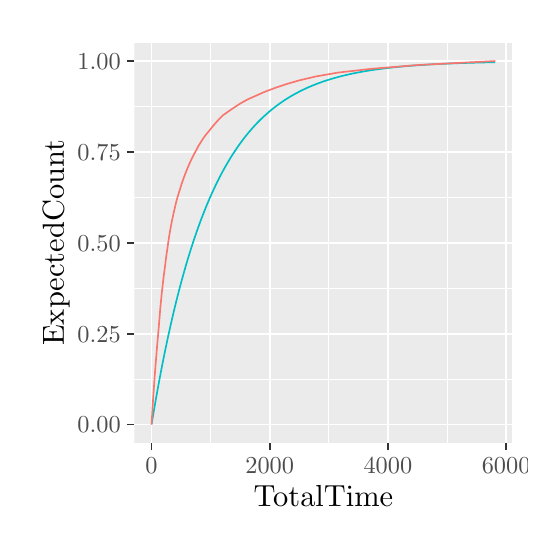
\begin{tikzpicture}[x=1pt,y=1pt]
\definecolor{fillColor}{RGB}{255,255,255}
\path[use as bounding box,fill=fillColor,fill opacity=0.00] (0,0) rectangle (180.67,180.67);
\begin{scope}
\path[clip] (  0.00,  0.00) rectangle (180.67,180.67);
\definecolor{drawColor}{RGB}{255,255,255}
\definecolor{fillColor}{RGB}{255,255,255}

\path[draw=drawColor,line width= 0.6pt,line join=round,line cap=round,fill=fillColor] (  0.00,  0.00) rectangle (180.68,180.68);
\end{scope}
\begin{scope}
\path[clip] ( 38.56, 30.69) rectangle (175.17,175.17);
\definecolor{fillColor}{gray}{0.92}

\path[fill=fillColor] ( 38.56, 30.69) rectangle (175.18,175.17);
\definecolor{drawColor}{RGB}{255,255,255}

\path[draw=drawColor,line width= 0.3pt,line join=round] ( 38.56, 53.67) --
	(175.17, 53.67);

\path[draw=drawColor,line width= 0.3pt,line join=round] ( 38.56, 86.51) --
	(175.17, 86.51);

\path[draw=drawColor,line width= 0.3pt,line join=round] ( 38.56,119.35) --
	(175.17,119.35);

\path[draw=drawColor,line width= 0.3pt,line join=round] ( 38.56,152.19) --
	(175.17,152.19);

\path[draw=drawColor,line width= 0.3pt,line join=round] ( 66.12, 30.69) --
	( 66.12,175.17);

\path[draw=drawColor,line width= 0.3pt,line join=round] (108.82, 30.69) --
	(108.82,175.17);

\path[draw=drawColor,line width= 0.3pt,line join=round] (151.52, 30.69) --
	(151.52,175.17);

\path[draw=drawColor,line width= 0.6pt,line join=round] ( 38.56, 37.25) --
	(175.17, 37.25);

\path[draw=drawColor,line width= 0.6pt,line join=round] ( 38.56, 70.09) --
	(175.17, 70.09);

\path[draw=drawColor,line width= 0.6pt,line join=round] ( 38.56,102.93) --
	(175.17,102.93);

\path[draw=drawColor,line width= 0.6pt,line join=round] ( 38.56,135.77) --
	(175.17,135.77);

\path[draw=drawColor,line width= 0.6pt,line join=round] ( 38.56,168.61) --
	(175.17,168.61);

\path[draw=drawColor,line width= 0.6pt,line join=round] ( 44.77, 30.69) --
	( 44.77,175.17);

\path[draw=drawColor,line width= 0.6pt,line join=round] ( 87.47, 30.69) --
	( 87.47,175.17);

\path[draw=drawColor,line width= 0.6pt,line join=round] (130.17, 30.69) --
	(130.17,175.17);

\path[draw=drawColor,line width= 0.6pt,line join=round] (172.88, 30.69) --
	(172.88,175.17);
\definecolor{drawColor}{RGB}{0,191,196}

\path[draw=drawColor,line width= 0.6pt,line join=round] ( 44.79, 37.38) --
	( 44.81, 37.51) --
	( 44.83, 37.64) --
	( 44.85, 37.77) --
	( 44.87, 37.90) --
	( 44.89, 38.03) --
	( 44.91, 38.16) --
	( 44.94, 38.29) --
	( 44.96, 38.42) --
	( 44.98, 38.55) --
	( 45.00, 38.68) --
	( 45.02, 38.80) --
	( 45.04, 38.93) --
	( 45.06, 39.06) --
	( 45.09, 39.19) --
	( 45.11, 39.32) --
	( 45.13, 39.45) --
	( 45.15, 39.57) --
	( 45.17, 39.70) --
	( 45.19, 39.83) --
	( 45.21, 39.96) --
	( 45.23, 40.08) --
	( 45.26, 40.21) --
	( 45.28, 40.34) --
	( 45.30, 40.46) --
	( 45.32, 40.59) --
	( 45.34, 40.72) --
	( 45.36, 40.84) --
	( 45.38, 40.97) --
	( 45.41, 41.10) --
	( 45.43, 41.22) --
	( 45.45, 41.35) --
	( 45.47, 41.48) --
	( 45.49, 41.60) --
	( 45.51, 41.73) --
	( 45.53, 41.85) --
	( 45.56, 41.98) --
	( 45.58, 42.10) --
	( 45.60, 42.23) --
	( 45.62, 42.35) --
	( 45.64, 42.48) --
	( 45.66, 42.60) --
	( 45.68, 42.73) --
	( 45.70, 42.85) --
	( 45.73, 42.98) --
	( 45.75, 43.10) --
	( 45.77, 43.23) --
	( 45.79, 43.35) --
	( 45.81, 43.47) --
	( 45.83, 43.60) --
	( 45.85, 43.72) --
	( 45.88, 43.84) --
	( 45.90, 43.97) --
	( 45.92, 44.09) --
	( 45.94, 44.21) --
	( 45.96, 44.34) --
	( 45.98, 44.46) --
	( 46.00, 44.58) --
	( 46.02, 44.71) --
	( 46.05, 44.83) --
	( 46.07, 44.95) --
	( 46.09, 45.07) --
	( 46.11, 45.20) --
	( 46.13, 45.32) --
	( 46.15, 45.44) --
	( 46.17, 45.56) --
	( 46.20, 45.68) --
	( 46.22, 45.81) --
	( 46.24, 45.93) --
	( 46.26, 46.05) --
	( 46.28, 46.17) --
	( 46.30, 46.29) --
	( 46.32, 46.41) --
	( 46.35, 46.53) --
	( 46.37, 46.65) --
	( 46.39, 46.77) --
	( 46.41, 46.89) --
	( 46.43, 47.01) --
	( 46.45, 47.14) --
	( 46.47, 47.26) --
	( 46.49, 47.38) --
	( 46.52, 47.50) --
	( 46.54, 47.62) --
	( 46.56, 47.74) --
	( 46.58, 47.85) --
	( 46.60, 47.97) --
	( 46.62, 48.09) --
	( 46.64, 48.21) --
	( 46.67, 48.33) --
	( 46.69, 48.45) --
	( 46.71, 48.57) --
	( 46.73, 48.69) --
	( 46.75, 48.81) --
	( 46.77, 48.93) --
	( 46.79, 49.04) --
	( 46.81, 49.16) --
	( 46.84, 49.28) --
	( 46.86, 49.40) --
	( 46.88, 49.52) --
	( 46.90, 49.63) --
	( 46.92, 49.75) --
	( 46.94, 49.87) --
	( 46.96, 49.99) --
	( 46.99, 50.10) --
	( 47.01, 50.22) --
	( 47.03, 50.34) --
	( 47.05, 50.46) --
	( 47.07, 50.57) --
	( 47.09, 50.69) --
	( 47.11, 50.81) --
	( 47.14, 50.92) --
	( 47.16, 51.04) --
	( 47.18, 51.16) --
	( 47.20, 51.27) --
	( 47.22, 51.39) --
	( 47.24, 51.50) --
	( 47.26, 51.62) --
	( 47.28, 51.74) --
	( 47.31, 51.85) --
	( 47.33, 51.97) --
	( 47.35, 52.08) --
	( 47.37, 52.20) --
	( 47.39, 52.31) --
	( 47.41, 52.43) --
	( 47.43, 52.54) --
	( 47.46, 52.66) --
	( 47.48, 52.77) --
	( 47.50, 52.89) --
	( 47.52, 53.00) --
	( 47.54, 53.12) --
	( 47.56, 53.23) --
	( 47.58, 53.34) --
	( 47.60, 53.46) --
	( 47.63, 53.57) --
	( 47.65, 53.69) --
	( 47.67, 53.80) --
	( 47.69, 53.91) --
	( 47.71, 54.03) --
	( 47.73, 54.14) --
	( 47.75, 54.25) --
	( 47.78, 54.37) --
	( 47.80, 54.48) --
	( 47.82, 54.59) --
	( 47.84, 54.71) --
	( 47.86, 54.82) --
	( 47.88, 54.93) --
	( 47.90, 55.04) --
	( 47.93, 55.16) --
	( 47.95, 55.27) --
	( 47.97, 55.38) --
	( 47.99, 55.49) --
	( 48.01, 55.60) --
	( 48.03, 55.72) --
	( 48.05, 55.83) --
	( 48.07, 55.94) --
	( 48.10, 56.05) --
	( 48.12, 56.16) --
	( 48.14, 56.27) --
	( 48.16, 56.38) --
	( 48.18, 56.50) --
	( 48.20, 56.61) --
	( 48.22, 56.72) --
	( 48.25, 56.83) --
	( 48.27, 56.94) --
	( 48.29, 57.05) --
	( 48.31, 57.16) --
	( 48.33, 57.27) --
	( 48.35, 57.38) --
	( 48.37, 57.49) --
	( 48.39, 57.60) --
	( 48.42, 57.71) --
	( 48.44, 57.82) --
	( 48.46, 57.93) --
	( 48.48, 58.04) --
	( 48.50, 58.15) --
	( 48.52, 58.26) --
	( 48.54, 58.37) --
	( 48.57, 58.48) --
	( 48.59, 58.58) --
	( 48.61, 58.69) --
	( 48.63, 58.80) --
	( 48.65, 58.91) --
	( 48.67, 59.02) --
	( 48.69, 59.13) --
	( 48.72, 59.24) --
	( 48.74, 59.34) --
	( 48.76, 59.45) --
	( 48.78, 59.56) --
	( 48.80, 59.67) --
	( 48.82, 59.78) --
	( 48.84, 59.88) --
	( 48.86, 59.99) --
	( 48.89, 60.10) --
	( 48.91, 60.21) --
	( 48.93, 60.31) --
	( 48.95, 60.42) --
	( 48.97, 60.53) --
	( 48.99, 60.64) --
	( 49.01, 60.74) --
	( 49.04, 60.85) --
	( 49.06, 60.96) --
	( 49.08, 61.06) --
	( 49.10, 61.17) --
	( 49.12, 61.27) --
	( 49.14, 61.38) --
	( 49.16, 61.49) --
	( 49.18, 61.59) --
	( 49.21, 61.70) --
	( 49.23, 61.80) --
	( 49.25, 61.91) --
	( 49.27, 62.02) --
	( 49.29, 62.12) --
	( 49.31, 62.23) --
	( 49.33, 62.33) --
	( 49.36, 62.44) --
	( 49.38, 62.54) --
	( 49.40, 62.65) --
	( 49.42, 62.75) --
	( 49.44, 62.86) --
	( 49.46, 62.96) --
	( 49.48, 63.07) --
	( 49.51, 63.17) --
	( 49.53, 63.27) --
	( 49.55, 63.38) --
	( 49.57, 63.48) --
	( 49.59, 63.59) --
	( 49.61, 63.69) --
	( 49.63, 63.79) --
	( 49.65, 63.90) --
	( 49.68, 64.00) --
	( 49.70, 64.11) --
	( 49.72, 64.21) --
	( 49.74, 64.31) --
	( 49.76, 64.42) --
	( 49.78, 64.52) --
	( 49.80, 64.62) --
	( 49.83, 64.72) --
	( 49.85, 64.83) --
	( 49.87, 64.93) --
	( 49.89, 65.03) --
	( 49.91, 65.13) --
	( 49.93, 65.24) --
	( 49.95, 65.34) --
	( 49.97, 65.44) --
	( 50.00, 65.54) --
	( 50.02, 65.65) --
	( 50.04, 65.75) --
	( 50.06, 65.85) --
	( 50.08, 65.95) --
	( 50.10, 66.05) --
	( 50.12, 66.15) --
	( 50.15, 66.26) --
	( 50.17, 66.36) --
	( 50.19, 66.46) --
	( 50.21, 66.56) --
	( 50.23, 66.66) --
	( 50.25, 66.76) --
	( 50.27, 66.86) --
	( 50.30, 66.96) --
	( 50.32, 67.06) --
	( 50.34, 67.16) --
	( 50.36, 67.26) --
	( 50.38, 67.36) --
	( 50.40, 67.46) --
	( 50.42, 67.56) --
	( 50.44, 67.66) --
	( 50.47, 67.76) --
	( 50.49, 67.86) --
	( 50.51, 67.96) --
	( 50.53, 68.06) --
	( 50.55, 68.16) --
	( 50.57, 68.26) --
	( 50.59, 68.36) --
	( 50.62, 68.46) --
	( 50.64, 68.56) --
	( 50.66, 68.66) --
	( 50.68, 68.76) --
	( 50.70, 68.86) --
	( 50.72, 68.96) --
	( 50.74, 69.05) --
	( 50.76, 69.15) --
	( 50.79, 69.25) --
	( 50.81, 69.35) --
	( 50.83, 69.45) --
	( 50.85, 69.55) --
	( 50.87, 69.64) --
	( 50.89, 69.74) --
	( 50.91, 69.84) --
	( 50.94, 69.94) --
	( 50.96, 70.03) --
	( 50.98, 70.13) --
	( 51.00, 70.23) --
	( 51.02, 70.33) --
	( 51.04, 70.42) --
	( 51.06, 70.52) --
	( 51.09, 70.62) --
	( 51.11, 70.72) --
	( 51.13, 70.81) --
	( 51.15, 70.91) --
	( 51.17, 71.01) --
	( 51.19, 71.10) --
	( 51.21, 71.20) --
	( 51.23, 71.30) --
	( 51.26, 71.39) --
	( 51.28, 71.49) --
	( 51.30, 71.58) --
	( 51.32, 71.68) --
	( 51.34, 71.78) --
	( 51.36, 71.87) --
	( 51.38, 71.97) --
	( 51.41, 72.06) --
	( 51.43, 72.16) --
	( 51.45, 72.25) --
	( 51.47, 72.35) --
	( 51.49, 72.44) --
	( 51.51, 72.54) --
	( 51.53, 72.63) --
	( 51.55, 72.73) --
	( 51.58, 72.82) --
	( 51.60, 72.92) --
	( 51.62, 73.01) --
	( 51.64, 73.11) --
	( 51.66, 73.20) --
	( 51.68, 73.30) --
	( 51.70, 73.39) --
	( 51.73, 73.49) --
	( 51.75, 73.58) --
	( 51.77, 73.67) --
	( 51.79, 73.77) --
	( 51.81, 73.86) --
	( 51.83, 73.96) --
	( 51.85, 74.05) --
	( 51.88, 74.14) --
	( 51.90, 74.24) --
	( 51.92, 74.33) --
	( 51.94, 74.42) --
	( 51.96, 74.52) --
	( 51.98, 74.61) --
	( 52.00, 74.70) --
	( 52.02, 74.80) --
	( 52.05, 74.89) --
	( 52.07, 74.98) --
	( 52.09, 75.07) --
	( 52.11, 75.17) --
	( 52.13, 75.26) --
	( 52.15, 75.35) --
	( 52.17, 75.44) --
	( 52.20, 75.54) --
	( 52.22, 75.63) --
	( 52.24, 75.72) --
	( 52.26, 75.81) --
	( 52.28, 75.90) --
	( 52.30, 75.99) --
	( 52.32, 76.09) --
	( 52.34, 76.18) --
	( 52.37, 76.27) --
	( 52.39, 76.36) --
	( 52.41, 76.45) --
	( 52.43, 76.54) --
	( 52.45, 76.63) --
	( 52.47, 76.73) --
	( 52.49, 76.82) --
	( 52.52, 76.91) --
	( 52.54, 77.00) --
	( 52.56, 77.09) --
	( 52.58, 77.18) --
	( 52.60, 77.27) --
	( 52.62, 77.36) --
	( 52.64, 77.45) --
	( 52.67, 77.54) --
	( 52.69, 77.63) --
	( 52.71, 77.72) --
	( 52.73, 77.81) --
	( 52.75, 77.90) --
	( 52.77, 77.99) --
	( 52.79, 78.08) --
	( 52.81, 78.17) --
	( 52.84, 78.26) --
	( 52.86, 78.35) --
	( 52.88, 78.44) --
	( 52.90, 78.53) --
	( 52.92, 78.62) --
	( 52.94, 78.70) --
	( 52.96, 78.79) --
	( 52.99, 78.88) --
	( 53.01, 78.97) --
	( 53.03, 79.06) --
	( 53.05, 79.15) --
	( 53.07, 79.24) --
	( 53.09, 79.33) --
	( 53.11, 79.41) --
	( 53.13, 79.50) --
	( 53.16, 79.59) --
	( 53.18, 79.68) --
	( 53.20, 79.77) --
	( 53.22, 79.85) --
	( 53.24, 79.94) --
	( 53.26, 80.03) --
	( 53.28, 80.12) --
	( 53.31, 80.21) --
	( 53.33, 80.29) --
	( 53.35, 80.38) --
	( 53.37, 80.47) --
	( 53.39, 80.55) --
	( 53.41, 80.64) --
	( 53.43, 80.73) --
	( 53.46, 80.82) --
	( 53.48, 80.90) --
	( 53.50, 80.99) --
	( 53.52, 81.08) --
	( 53.54, 81.16) --
	( 53.56, 81.25) --
	( 53.58, 81.34) --
	( 53.60, 81.42) --
	( 53.63, 81.51) --
	( 53.65, 81.59) --
	( 53.67, 81.68) --
	( 53.69, 81.77) --
	( 53.71, 81.85) --
	( 53.73, 81.94) --
	( 53.75, 82.02) --
	( 53.78, 82.11) --
	( 53.80, 82.20) --
	( 53.82, 82.28) --
	( 53.84, 82.37) --
	( 53.86, 82.45) --
	( 53.88, 82.54) --
	( 53.90, 82.62) --
	( 53.93, 82.71) --
	( 53.95, 82.79) --
	( 53.97, 82.88) --
	( 53.99, 82.96) --
	( 54.01, 83.05) --
	( 54.03, 83.13) --
	( 54.05, 83.22) --
	( 54.07, 83.30) --
	( 54.10, 83.38) --
	( 54.12, 83.47) --
	( 54.14, 83.55) --
	( 54.16, 83.64) --
	( 54.18, 83.72) --
	( 54.20, 83.81) --
	( 54.22, 83.89) --
	( 54.25, 83.97) --
	( 54.27, 84.06) --
	( 54.29, 84.14) --
	( 54.31, 84.22) --
	( 54.33, 84.31) --
	( 54.35, 84.39) --
	( 54.37, 84.47) --
	( 54.39, 84.56) --
	( 54.42, 84.64) --
	( 54.44, 84.72) --
	( 54.46, 84.81) --
	( 54.48, 84.89) --
	( 54.50, 84.97) --
	( 54.52, 85.06) --
	( 54.54, 85.14) --
	( 54.57, 85.22) --
	( 54.59, 85.30) --
	( 54.61, 85.39) --
	( 54.63, 85.47) --
	( 54.65, 85.55) --
	( 54.67, 85.63) --
	( 54.69, 85.71) --
	( 54.72, 85.80) --
	( 54.74, 85.88) --
	( 54.76, 85.96) --
	( 54.78, 86.04) --
	( 54.80, 86.12) --
	( 54.82, 86.21) --
	( 54.84, 86.29) --
	( 54.86, 86.37) --
	( 54.89, 86.45) --
	( 54.91, 86.53) --
	( 54.93, 86.61) --
	( 54.95, 86.69) --
	( 54.97, 86.77) --
	( 54.99, 86.86) --
	( 55.01, 86.94) --
	( 55.04, 87.02) --
	( 55.06, 87.10) --
	( 55.08, 87.18) --
	( 55.10, 87.26) --
	( 55.12, 87.34) --
	( 55.14, 87.42) --
	( 55.16, 87.50) --
	( 55.18, 87.58) --
	( 55.21, 87.66) --
	( 55.23, 87.74) --
	( 55.25, 87.82) --
	( 55.27, 87.90) --
	( 55.29, 87.98) --
	( 55.31, 88.06) --
	( 55.33, 88.14) --
	( 55.36, 88.22) --
	( 55.38, 88.30) --
	( 55.40, 88.38) --
	( 55.42, 88.46) --
	( 55.44, 88.54) --
	( 55.46, 88.62) --
	( 55.48, 88.70) --
	( 55.51, 88.78) --
	( 55.53, 88.85) --
	( 55.55, 88.93) --
	( 55.57, 89.01) --
	( 55.59, 89.09) --
	( 55.61, 89.17) --
	( 55.63, 89.25) --
	( 55.65, 89.33) --
	( 55.68, 89.41) --
	( 55.70, 89.48) --
	( 55.72, 89.56) --
	( 55.74, 89.64) --
	( 55.76, 89.72) --
	( 55.78, 89.80) --
	( 55.80, 89.87) --
	( 55.83, 89.95) --
	( 55.85, 90.03) --
	( 55.87, 90.11) --
	( 55.89, 90.19) --
	( 55.91, 90.26) --
	( 55.93, 90.34) --
	( 55.95, 90.42) --
	( 55.97, 90.50) --
	( 56.00, 90.57) --
	( 56.02, 90.65) --
	( 56.04, 90.73) --
	( 56.06, 90.80) --
	( 56.08, 90.88) --
	( 56.10, 90.96) --
	( 56.12, 91.03) --
	( 56.15, 91.11) --
	( 56.17, 91.19) --
	( 56.19, 91.26) --
	( 56.21, 91.34) --
	( 56.23, 91.42) --
	( 56.25, 91.49) --
	( 56.27, 91.57) --
	( 56.30, 91.65) --
	( 56.32, 91.72) --
	( 56.34, 91.80) --
	( 56.36, 91.87) --
	( 56.38, 91.95) --
	( 56.40, 92.03) --
	( 56.42, 92.10) --
	( 56.44, 92.18) --
	( 56.47, 92.25) --
	( 56.49, 92.33) --
	( 56.51, 92.40) --
	( 56.53, 92.48) --
	( 56.55, 92.56) --
	( 56.57, 92.63) --
	( 56.59, 92.71) --
	( 56.62, 92.78) --
	( 56.64, 92.86) --
	( 56.66, 92.93) --
	( 56.68, 93.01) --
	( 56.70, 93.08) --
	( 56.72, 93.16) --
	( 56.74, 93.23) --
	( 56.76, 93.30) --
	( 56.79, 93.38) --
	( 56.81, 93.45) --
	( 56.83, 93.53) --
	( 56.85, 93.60) --
	( 56.87, 93.68) --
	( 56.89, 93.75) --
	( 56.91, 93.82) --
	( 56.94, 93.90) --
	( 56.96, 93.97) --
	( 56.98, 94.05) --
	( 57.00, 94.12) --
	( 57.02, 94.19) --
	( 57.04, 94.27) --
	( 57.06, 94.34) --
	( 57.09, 94.41) --
	( 57.11, 94.49) --
	( 57.13, 94.56) --
	( 57.15, 94.63) --
	( 57.17, 94.71) --
	( 57.19, 94.78) --
	( 57.21, 94.85) --
	( 57.23, 94.93) --
	( 57.26, 95.00) --
	( 57.28, 95.07) --
	( 57.30, 95.15) --
	( 57.32, 95.22) --
	( 57.34, 95.29) --
	( 57.36, 95.36) --
	( 57.38, 95.44) --
	( 57.41, 95.51) --
	( 57.43, 95.58) --
	( 57.45, 95.65) --
	( 57.47, 95.73) --
	( 57.49, 95.80) --
	( 57.51, 95.87) --
	( 57.53, 95.94) --
	( 57.55, 96.01) --
	( 57.58, 96.08) --
	( 57.60, 96.16) --
	( 57.62, 96.23) --
	( 57.64, 96.30) --
	( 57.66, 96.37) --
	( 57.68, 96.44) --
	( 57.70, 96.51) --
	( 57.73, 96.59) --
	( 57.75, 96.66) --
	( 57.77, 96.73) --
	( 57.79, 96.80) --
	( 57.81, 96.87) --
	( 57.83, 96.94) --
	( 57.85, 97.01) --
	( 57.88, 97.08) --
	( 57.90, 97.15) --
	( 57.92, 97.22) --
	( 57.94, 97.30) --
	( 57.96, 97.37) --
	( 57.98, 97.44) --
	( 58.00, 97.51) --
	( 58.02, 97.58) --
	( 58.05, 97.65) --
	( 58.07, 97.72) --
	( 58.09, 97.79) --
	( 58.11, 97.86) --
	( 58.13, 97.93) --
	( 58.15, 98.00) --
	( 58.17, 98.07) --
	( 58.20, 98.14) --
	( 58.22, 98.21) --
	( 58.24, 98.28) --
	( 58.26, 98.35) --
	( 58.28, 98.42) --
	( 58.30, 98.49) --
	( 58.32, 98.55) --
	( 58.34, 98.62) --
	( 58.37, 98.69) --
	( 58.39, 98.76) --
	( 58.41, 98.83) --
	( 58.43, 98.90) --
	( 58.45, 98.97) --
	( 58.47, 99.04) --
	( 58.49, 99.11) --
	( 58.52, 99.18) --
	( 58.54, 99.24) --
	( 58.56, 99.31) --
	( 58.58, 99.38) --
	( 58.60, 99.45) --
	( 58.62, 99.52) --
	( 58.64, 99.59) --
	( 58.67, 99.66) --
	( 58.69, 99.72) --
	( 58.71, 99.79) --
	( 58.73, 99.86) --
	( 58.75, 99.93) --
	( 58.77,100.00) --
	( 58.79,100.06) --
	( 58.81,100.13) --
	( 58.84,100.20) --
	( 58.86,100.27) --
	( 58.88,100.33) --
	( 58.90,100.40) --
	( 58.92,100.47) --
	( 58.94,100.54) --
	( 58.96,100.60) --
	( 58.99,100.67) --
	( 59.01,100.74) --
	( 59.03,100.81) --
	( 59.05,100.87) --
	( 59.07,100.94) --
	( 59.09,101.01) --
	( 59.11,101.07) --
	( 59.13,101.14) --
	( 59.16,101.21) --
	( 59.18,101.27) --
	( 59.20,101.34) --
	( 59.22,101.41) --
	( 59.24,101.47) --
	( 59.26,101.54) --
	( 59.28,101.61) --
	( 59.31,101.67) --
	( 59.33,101.74) --
	( 59.35,101.81) --
	( 59.37,101.87) --
	( 59.39,101.94) --
	( 59.41,102.00) --
	( 59.43,102.07) --
	( 59.46,102.14) --
	( 59.48,102.20) --
	( 59.50,102.27) --
	( 59.52,102.33) --
	( 59.54,102.40) --
	( 59.56,102.46) --
	( 59.58,102.53) --
	( 59.60,102.59) --
	( 59.63,102.66) --
	( 59.65,102.73) --
	( 59.67,102.79) --
	( 59.69,102.86) --
	( 59.71,102.92) --
	( 59.73,102.99) --
	( 59.75,103.05) --
	( 59.78,103.12) --
	( 59.80,103.18) --
	( 59.82,103.25) --
	( 59.84,103.31) --
	( 59.86,103.37) --
	( 59.88,103.44) --
	( 59.90,103.50) --
	( 59.92,103.57) --
	( 59.95,103.63) --
	( 59.97,103.70) --
	( 59.99,103.76) --
	( 60.01,103.82) --
	( 60.03,103.89) --
	( 60.05,103.95) --
	( 60.07,104.02) --
	( 60.10,104.08) --
	( 60.12,104.14) --
	( 60.14,104.21) --
	( 60.16,104.27) --
	( 60.18,104.34) --
	( 60.20,104.40) --
	( 60.22,104.46) --
	( 60.25,104.53) --
	( 60.27,104.59) --
	( 60.29,104.65) --
	( 60.31,104.72) --
	( 60.33,104.78) --
	( 60.35,104.84) --
	( 60.37,104.91) --
	( 60.39,104.97) --
	( 60.42,105.03) --
	( 60.44,105.09) --
	( 60.46,105.16) --
	( 60.48,105.22) --
	( 60.50,105.28) --
	( 60.52,105.35) --
	( 60.54,105.41) --
	( 60.57,105.47) --
	( 60.59,105.53) --
	( 60.61,105.60) --
	( 60.63,105.66) --
	( 60.65,105.72) --
	( 60.67,105.78) --
	( 60.69,105.85) --
	( 60.71,105.91) --
	( 60.74,105.97) --
	( 60.76,106.03) --
	( 60.78,106.09) --
	( 60.80,106.15) --
	( 60.82,106.22) --
	( 60.84,106.28) --
	( 60.86,106.34) --
	( 60.89,106.40) --
	( 60.91,106.46) --
	( 60.93,106.52) --
	( 60.95,106.59) --
	( 60.97,106.65) --
	( 60.99,106.71) --
	( 61.01,106.77) --
	( 61.04,106.83) --
	( 61.06,106.89) --
	( 61.08,106.95) --
	( 61.10,107.01) --
	( 61.12,107.08) --
	( 61.14,107.14) --
	( 61.16,107.20) --
	( 61.18,107.26) --
	( 61.21,107.32) --
	( 61.23,107.38) --
	( 61.25,107.44) --
	( 61.27,107.50) --
	( 61.29,107.56) --
	( 61.31,107.62) --
	( 61.33,107.68) --
	( 61.36,107.74) --
	( 61.38,107.80) --
	( 61.40,107.86) --
	( 61.42,107.92) --
	( 61.44,107.98) --
	( 61.46,108.04) --
	( 61.48,108.10) --
	( 61.50,108.16) --
	( 61.53,108.22) --
	( 61.55,108.28) --
	( 61.57,108.34) --
	( 61.59,108.40) --
	( 61.61,108.46) --
	( 61.63,108.52) --
	( 61.65,108.58) --
	( 61.68,108.64) --
	( 61.70,108.70) --
	( 61.72,108.76) --
	( 61.74,108.82) --
	( 61.76,108.88) --
	( 61.78,108.94) --
	( 61.80,108.99) --
	( 61.83,109.05) --
	( 61.85,109.11) --
	( 61.87,109.17) --
	( 61.89,109.23) --
	( 61.91,109.29) --
	( 61.93,109.35) --
	( 61.95,109.41) --
	( 61.97,109.46) --
	( 62.00,109.52) --
	( 62.02,109.58) --
	( 62.04,109.64) --
	( 62.06,109.70) --
	( 62.08,109.76) --
	( 62.10,109.81) --
	( 62.12,109.87) --
	( 62.15,109.93) --
	( 62.17,109.99) --
	( 62.19,110.05) --
	( 62.21,110.11) --
	( 62.23,110.16) --
	( 62.25,110.22) --
	( 62.27,110.28) --
	( 62.29,110.34) --
	( 62.32,110.39) --
	( 62.34,110.45) --
	( 62.36,110.51) --
	( 62.38,110.57) --
	( 62.40,110.62) --
	( 62.42,110.68) --
	( 62.44,110.74) --
	( 62.47,110.80) --
	( 62.49,110.85) --
	( 62.51,110.91) --
	( 62.53,110.97) --
	( 62.55,111.02) --
	( 62.57,111.08) --
	( 62.59,111.14) --
	( 62.62,111.20) --
	( 62.64,111.25) --
	( 62.66,111.31) --
	( 62.68,111.37) --
	( 62.70,111.42) --
	( 62.72,111.48) --
	( 62.74,111.54) --
	( 62.76,111.59) --
	( 62.79,111.65) --
	( 62.81,111.70) --
	( 62.83,111.76) --
	( 62.85,111.82) --
	( 62.87,111.87) --
	( 62.89,111.93) --
	( 62.91,111.99) --
	( 62.94,112.04) --
	( 62.96,112.10) --
	( 62.98,112.15) --
	( 63.00,112.21) --
	( 63.02,112.27) --
	( 63.04,112.32) --
	( 63.06,112.38) --
	( 63.08,112.43) --
	( 63.11,112.49) --
	( 63.13,112.54) --
	( 63.15,112.60) --
	( 63.17,112.65) --
	( 63.19,112.71) --
	( 63.21,112.76) --
	( 63.23,112.82) --
	( 63.26,112.88) --
	( 63.28,112.93) --
	( 63.30,112.99) --
	( 63.32,113.04) --
	( 63.34,113.10) --
	( 63.36,113.15) --
	( 63.38,113.21) --
	( 63.41,113.26) --
	( 63.43,113.31) --
	( 63.45,113.37) --
	( 63.47,113.42) --
	( 63.49,113.48) --
	( 63.51,113.53) --
	( 63.53,113.59) --
	( 63.55,113.64) --
	( 63.58,113.70) --
	( 63.60,113.75) --
	( 63.62,113.81) --
	( 63.64,113.86) --
	( 63.66,113.91) --
	( 63.68,113.97) --
	( 63.70,114.02) --
	( 63.73,114.08) --
	( 63.75,114.13) --
	( 63.77,114.18) --
	( 63.79,114.24) --
	( 63.81,114.29) --
	( 63.83,114.35) --
	( 63.85,114.40) --
	( 63.88,114.45) --
	( 63.90,114.51) --
	( 63.92,114.56) --
	( 63.94,114.61) --
	( 63.96,114.67) --
	( 63.98,114.72) --
	( 64.00,114.77) --
	( 64.02,114.83) --
	( 64.05,114.88) --
	( 64.07,114.93) --
	( 64.09,114.99) --
	( 64.11,115.04) --
	( 64.13,115.09) --
	( 64.15,115.15) --
	( 64.17,115.20) --
	( 64.20,115.25) --
	( 64.22,115.30) --
	( 64.24,115.36) --
	( 64.26,115.41) --
	( 64.28,115.46) --
	( 64.30,115.51) --
	( 64.32,115.57) --
	( 64.34,115.62) --
	( 64.37,115.67) --
	( 64.39,115.72) --
	( 64.41,115.78) --
	( 64.43,115.83) --
	( 64.45,115.88) --
	( 64.47,115.93) --
	( 64.49,115.99) --
	( 64.52,116.04) --
	( 64.54,116.09) --
	( 64.56,116.14) --
	( 64.58,116.19) --
	( 64.60,116.25) --
	( 64.62,116.30) --
	( 64.64,116.35) --
	( 64.67,116.40) --
	( 64.69,116.45) --
	( 64.71,116.50) --
	( 64.73,116.56) --
	( 64.75,116.61) --
	( 64.77,116.66) --
	( 64.79,116.71) --
	( 64.81,116.76) --
	( 64.84,116.81) --
	( 64.86,116.86) --
	( 64.88,116.91) --
	( 64.90,116.97) --
	( 64.92,117.02) --
	( 64.94,117.07) --
	( 64.96,117.12) --
	( 64.99,117.17) --
	( 65.01,117.22) --
	( 65.03,117.27) --
	( 65.05,117.32) --
	( 65.07,117.37) --
	( 65.09,117.42) --
	( 65.11,117.47) --
	( 65.13,117.53) --
	( 65.16,117.58) --
	( 65.18,117.63) --
	( 65.20,117.68) --
	( 65.22,117.73) --
	( 65.24,117.78) --
	( 65.26,117.83) --
	( 65.28,117.88) --
	( 65.31,117.93) --
	( 65.33,117.98) --
	( 65.35,118.03) --
	( 65.37,118.08) --
	( 65.39,118.13) --
	( 65.41,118.18) --
	( 65.43,118.23) --
	( 65.46,118.28) --
	( 65.48,118.33) --
	( 65.50,118.38) --
	( 65.52,118.43) --
	( 65.54,118.48) --
	( 65.56,118.53) --
	( 65.58,118.58) --
	( 65.60,118.63) --
	( 65.63,118.68) --
	( 65.65,118.72) --
	( 65.67,118.77) --
	( 65.69,118.82) --
	( 65.71,118.87) --
	( 65.73,118.92) --
	( 65.75,118.97) --
	( 65.78,119.02) --
	( 65.80,119.07) --
	( 65.82,119.12) --
	( 65.84,119.17) --
	( 65.86,119.22) --
	( 65.88,119.26) --
	( 65.90,119.31) --
	( 65.92,119.36) --
	( 65.95,119.41) --
	( 65.97,119.46) --
	( 65.99,119.51) --
	( 66.01,119.56) --
	( 66.03,119.61) --
	( 66.05,119.65) --
	( 66.07,119.70) --
	( 66.10,119.75) --
	( 66.12,119.80) --
	( 66.14,119.85) --
	( 66.16,119.90) --
	( 66.18,119.94) --
	( 66.20,119.99) --
	( 66.22,120.04) --
	( 66.25,120.09) --
	( 66.27,120.14) --
	( 66.29,120.18) --
	( 66.31,120.23) --
	( 66.33,120.28) --
	( 66.35,120.33) --
	( 66.37,120.38) --
	( 66.39,120.42) --
	( 66.42,120.47) --
	( 66.44,120.52) --
	( 66.46,120.57) --
	( 66.48,120.61) --
	( 66.50,120.66) --
	( 66.52,120.71) --
	( 66.54,120.76) --
	( 66.57,120.80) --
	( 66.59,120.85) --
	( 66.61,120.90) --
	( 66.63,120.95) --
	( 66.65,120.99) --
	( 66.67,121.04) --
	( 66.69,121.09) --
	( 66.71,121.13) --
	( 66.74,121.18) --
	( 66.76,121.23) --
	( 66.78,121.27) --
	( 66.80,121.32) --
	( 66.82,121.37) --
	( 66.84,121.41) --
	( 66.86,121.46) --
	( 66.89,121.51) --
	( 66.91,121.55) --
	( 66.93,121.60) --
	( 66.95,121.65) --
	( 66.97,121.69) --
	( 66.99,121.74) --
	( 67.01,121.79) --
	( 67.04,121.83) --
	( 67.06,121.88) --
	( 67.08,121.93) --
	( 67.10,121.97) --
	( 67.12,122.02) --
	( 67.14,122.06) --
	( 67.16,122.11) --
	( 67.18,122.16) --
	( 67.21,122.20) --
	( 67.23,122.25) --
	( 67.25,122.29) --
	( 67.27,122.34) --
	( 67.29,122.39) --
	( 67.31,122.43) --
	( 67.33,122.48) --
	( 67.36,122.52) --
	( 67.38,122.57) --
	( 67.40,122.61) --
	( 67.42,122.66) --
	( 67.44,122.71) --
	( 67.46,122.75) --
	( 67.48,122.80) --
	( 67.50,122.84) --
	( 67.53,122.89) --
	( 67.55,122.93) --
	( 67.57,122.98) --
	( 67.59,123.02) --
	( 67.61,123.07) --
	( 67.63,123.11) --
	( 67.65,123.16) --
	( 67.68,123.20) --
	( 67.70,123.25) --
	( 67.72,123.29) --
	( 67.74,123.34) --
	( 67.76,123.38) --
	( 67.78,123.43) --
	( 67.80,123.47) --
	( 67.83,123.52) --
	( 67.85,123.56) --
	( 67.87,123.60) --
	( 67.89,123.65) --
	( 67.91,123.69) --
	( 67.93,123.74) --
	( 67.95,123.78) --
	( 67.97,123.83) --
	( 68.00,123.87) --
	( 68.02,123.92) --
	( 68.04,123.96) --
	( 68.06,124.00) --
	( 68.08,124.05) --
	( 68.10,124.09) --
	( 68.12,124.14) --
	( 68.15,124.18) --
	( 68.17,124.22) --
	( 68.19,124.27) --
	( 68.21,124.31) --
	( 68.23,124.36) --
	( 68.25,124.40) --
	( 68.27,124.44) --
	( 68.29,124.49) --
	( 68.32,124.53) --
	( 68.34,124.57) --
	( 68.36,124.62) --
	( 68.38,124.66) --
	( 68.40,124.71) --
	( 68.42,124.75) --
	( 68.44,124.79) --
	( 68.47,124.84) --
	( 68.49,124.88) --
	( 68.51,124.92) --
	( 68.53,124.97) --
	( 68.55,125.01) --
	( 68.57,125.05) --
	( 68.59,125.09) --
	( 68.62,125.14) --
	( 68.64,125.18) --
	( 68.66,125.22) --
	( 68.68,125.27) --
	( 68.70,125.31) --
	( 68.72,125.35) --
	( 68.74,125.40) --
	( 68.76,125.44) --
	( 68.79,125.48) --
	( 68.81,125.52) --
	( 68.83,125.57) --
	( 68.85,125.61) --
	( 68.87,125.65) --
	( 68.89,125.69) --
	( 68.91,125.74) --
	( 68.94,125.78) --
	( 68.96,125.82) --
	( 68.98,125.86) --
	( 69.00,125.91) --
	( 69.02,125.95) --
	( 69.04,125.99) --
	( 69.06,126.03) --
	( 69.08,126.07) --
	( 69.11,126.12) --
	( 69.13,126.16) --
	( 69.15,126.20) --
	( 69.17,126.24) --
	( 69.19,126.28) --
	( 69.21,126.33) --
	( 69.23,126.37) --
	( 69.26,126.41) --
	( 69.28,126.45) --
	( 69.30,126.49) --
	( 69.32,126.53) --
	( 69.34,126.58) --
	( 69.36,126.62) --
	( 69.38,126.66) --
	( 69.41,126.70) --
	( 69.43,126.74) --
	( 69.45,126.78) --
	( 69.47,126.83) --
	( 69.49,126.87) --
	( 69.51,126.91) --
	( 69.53,126.95) --
	( 69.55,126.99) --
	( 69.58,127.03) --
	( 69.60,127.07) --
	( 69.62,127.11) --
	( 69.64,127.15) --
	( 69.66,127.20) --
	( 69.68,127.24) --
	( 69.70,127.28) --
	( 69.73,127.32) --
	( 69.75,127.36) --
	( 69.77,127.40) --
	( 69.79,127.44) --
	( 69.81,127.48) --
	( 69.83,127.52) --
	( 69.85,127.56) --
	( 69.87,127.60) --
	( 69.90,127.64) --
	( 69.92,127.69) --
	( 69.94,127.73) --
	( 69.96,127.77) --
	( 69.98,127.81) --
	( 70.00,127.85) --
	( 70.02,127.89) --
	( 70.05,127.93) --
	( 70.07,127.97) --
	( 70.09,128.01) --
	( 70.11,128.05) --
	( 70.13,128.09) --
	( 70.15,128.13) --
	( 70.17,128.17) --
	( 70.20,128.21) --
	( 70.22,128.25) --
	( 70.24,128.29) --
	( 70.26,128.33) --
	( 70.28,128.37) --
	( 70.30,128.41) --
	( 70.32,128.45) --
	( 70.34,128.49) --
	( 70.37,128.53) --
	( 70.39,128.57) --
	( 70.41,128.61) --
	( 70.43,128.65) --
	( 70.45,128.69) --
	( 70.47,128.72) --
	( 70.49,128.76) --
	( 70.52,128.80) --
	( 70.54,128.84) --
	( 70.56,128.88) --
	( 70.58,128.92) --
	( 70.60,128.96) --
	( 70.62,129.00) --
	( 70.64,129.04) --
	( 70.66,129.08) --
	( 70.69,129.12) --
	( 70.71,129.16) --
	( 70.73,129.20) --
	( 70.75,129.23) --
	( 70.77,129.27) --
	( 70.79,129.31) --
	( 70.81,129.35) --
	( 70.84,129.39) --
	( 70.86,129.43) --
	( 70.88,129.47) --
	( 70.90,129.51) --
	( 70.92,129.55) --
	( 70.94,129.58) --
	( 70.96,129.62) --
	( 70.99,129.66) --
	( 71.01,129.70) --
	( 71.03,129.74) --
	( 71.05,129.78) --
	( 71.07,129.82) --
	( 71.09,129.85) --
	( 71.11,129.89) --
	( 71.13,129.93) --
	( 71.16,129.97) --
	( 71.18,130.01) --
	( 71.20,130.05) --
	( 71.22,130.08) --
	( 71.24,130.12) --
	( 71.26,130.16) --
	( 71.28,130.20) --
	( 71.31,130.24) --
	( 71.33,130.27) --
	( 71.35,130.31) --
	( 71.37,130.35) --
	( 71.39,130.39) --
	( 71.41,130.42) --
	( 71.43,130.46) --
	( 71.45,130.50) --
	( 71.48,130.54) --
	( 71.50,130.58) --
	( 71.52,130.61) --
	( 71.54,130.65) --
	( 71.56,130.69) --
	( 71.58,130.73) --
	( 71.60,130.76) --
	( 71.63,130.80) --
	( 71.65,130.84) --
	( 71.67,130.88) --
	( 71.69,130.91) --
	( 71.71,130.95) --
	( 71.73,130.99) --
	( 71.75,131.02) --
	( 71.78,131.06) --
	( 71.80,131.10) --
	( 71.82,131.14) --
	( 71.84,131.17) --
	( 71.86,131.21) --
	( 71.88,131.25) --
	( 71.90,131.28) --
	( 71.92,131.32) --
	( 71.95,131.36) --
	( 71.97,131.40) --
	( 71.99,131.43) --
	( 72.01,131.47) --
	( 72.03,131.51) --
	( 72.05,131.54) --
	( 72.07,131.58) --
	( 72.10,131.62) --
	( 72.12,131.65) --
	( 72.14,131.69) --
	( 72.16,131.73) --
	( 72.18,131.76) --
	( 72.20,131.80) --
	( 72.22,131.83) --
	( 72.24,131.87) --
	( 72.27,131.91) --
	( 72.29,131.94) --
	( 72.31,131.98) --
	( 72.33,132.02) --
	( 72.35,132.05) --
	( 72.37,132.09) --
	( 72.39,132.12) --
	( 72.42,132.16) --
	( 72.44,132.20) --
	( 72.46,132.23) --
	( 72.48,132.27) --
	( 72.50,132.30) --
	( 72.52,132.34) --
	( 72.54,132.38) --
	( 72.57,132.41) --
	( 72.59,132.45) --
	( 72.61,132.48) --
	( 72.63,132.52) --
	( 72.65,132.56) --
	( 72.67,132.59) --
	( 72.69,132.63) --
	( 72.71,132.66) --
	( 72.74,132.70) --
	( 72.76,132.73) --
	( 72.78,132.77) --
	( 72.80,132.80) --
	( 72.82,132.84) --
	( 72.84,132.88) --
	( 72.86,132.91) --
	( 72.89,132.95) --
	( 72.91,132.98) --
	( 72.93,133.02) --
	( 72.95,133.05) --
	( 72.97,133.09) --
	( 72.99,133.12) --
	( 73.01,133.16) --
	( 73.03,133.19) --
	( 73.06,133.23) --
	( 73.08,133.26) --
	( 73.10,133.30) --
	( 73.12,133.33) --
	( 73.14,133.37) --
	( 73.16,133.40) --
	( 73.18,133.44) --
	( 73.21,133.47) --
	( 73.23,133.51) --
	( 73.25,133.54) --
	( 73.27,133.58) --
	( 73.29,133.61) --
	( 73.31,133.65) --
	( 73.33,133.68) --
	( 73.36,133.71) --
	( 73.38,133.75) --
	( 73.40,133.78) --
	( 73.42,133.82) --
	( 73.44,133.85) --
	( 73.46,133.89) --
	( 73.48,133.92) --
	( 73.50,133.96) --
	( 73.53,133.99) --
	( 73.55,134.02) --
	( 73.57,134.06) --
	( 73.59,134.09) --
	( 73.61,134.13) --
	( 73.63,134.16) --
	( 73.65,134.19) --
	( 73.68,134.23) --
	( 73.70,134.26) --
	( 73.72,134.30) --
	( 73.74,134.33) --
	( 73.76,134.36) --
	( 73.78,134.40) --
	( 73.80,134.43) --
	( 73.83,134.47) --
	( 73.85,134.50) --
	( 73.87,134.53) --
	( 73.89,134.57) --
	( 73.91,134.60) --
	( 73.93,134.63) --
	( 73.95,134.67) --
	( 73.97,134.70) --
	( 74.00,134.74) --
	( 74.02,134.77) --
	( 74.04,134.80) --
	( 74.06,134.84) --
	( 74.08,134.87) --
	( 74.10,134.90) --
	( 74.12,134.94) --
	( 74.15,134.97) --
	( 74.17,135.00) --
	( 74.19,135.04) --
	( 74.21,135.07) --
	( 74.23,135.10) --
	( 74.25,135.14) --
	( 74.27,135.17) --
	( 74.29,135.20) --
	( 74.32,135.23) --
	( 74.34,135.27) --
	( 74.36,135.30) --
	( 74.38,135.33) --
	( 74.40,135.37) --
	( 74.42,135.40) --
	( 74.44,135.43) --
	( 74.47,135.47) --
	( 74.49,135.50) --
	( 74.51,135.53) --
	( 74.53,135.56) --
	( 74.55,135.60) --
	( 74.57,135.63) --
	( 74.59,135.66) --
	( 74.62,135.69) --
	( 74.64,135.73) --
	( 74.66,135.76) --
	( 74.68,135.79) --
	( 74.70,135.82) --
	( 74.72,135.86) --
	( 74.74,135.89) --
	( 74.76,135.92) --
	( 74.79,135.95) --
	( 74.81,135.99) --
	( 74.83,136.02) --
	( 74.85,136.05) --
	( 74.87,136.08) --
	( 74.89,136.11) --
	( 74.91,136.15) --
	( 74.94,136.18) --
	( 74.96,136.21) --
	( 74.98,136.24) --
	( 75.00,136.28) --
	( 75.02,136.31) --
	( 75.04,136.34) --
	( 75.06,136.37) --
	( 75.08,136.40) --
	( 75.11,136.44) --
	( 75.13,136.47) --
	( 75.15,136.50) --
	( 75.17,136.53) --
	( 75.19,136.56) --
	( 75.21,136.59) --
	( 75.23,136.63) --
	( 75.26,136.66) --
	( 75.28,136.69) --
	( 75.30,136.72) --
	( 75.32,136.75) --
	( 75.34,136.78) --
	( 75.36,136.81) --
	( 75.38,136.85) --
	( 75.41,136.88) --
	( 75.43,136.91) --
	( 75.45,136.94) --
	( 75.47,136.97) --
	( 75.49,137.00) --
	( 75.51,137.03) --
	( 75.53,137.07) --
	( 75.55,137.10) --
	( 75.58,137.13) --
	( 75.60,137.16) --
	( 75.62,137.19) --
	( 75.64,137.22) --
	( 75.66,137.25) --
	( 75.68,137.28) --
	( 75.70,137.31) --
	( 75.73,137.35) --
	( 75.75,137.38) --
	( 75.77,137.41) --
	( 75.79,137.44) --
	( 75.81,137.47) --
	( 75.83,137.50) --
	( 75.85,137.53) --
	( 75.87,137.56) --
	( 75.90,137.59) --
	( 75.92,137.62) --
	( 75.94,137.65) --
	( 75.96,137.68) --
	( 75.98,137.71) --
	( 76.00,137.75) --
	( 76.02,137.78) --
	( 76.05,137.81) --
	( 76.07,137.84) --
	( 76.09,137.87) --
	( 76.11,137.90) --
	( 76.13,137.93) --
	( 76.15,137.96) --
	( 76.17,137.99) --
	( 76.20,138.02) --
	( 76.22,138.05) --
	( 76.24,138.08) --
	( 76.26,138.11) --
	( 76.28,138.14) --
	( 76.30,138.17) --
	( 76.32,138.20) --
	( 76.34,138.23) --
	( 76.37,138.26) --
	( 76.39,138.29) --
	( 76.41,138.32) --
	( 76.43,138.35) --
	( 76.45,138.38) --
	( 76.47,138.41) --
	( 76.49,138.44) --
	( 76.52,138.47) --
	( 76.54,138.50) --
	( 76.56,138.53) --
	( 76.58,138.56) --
	( 76.60,138.59) --
	( 76.62,138.62) --
	( 76.64,138.65) --
	( 76.66,138.68) --
	( 76.69,138.71) --
	( 76.71,138.74) --
	( 76.73,138.77) --
	( 76.75,138.80) --
	( 76.77,138.83) --
	( 76.79,138.86) --
	( 76.81,138.88) --
	( 76.84,138.91) --
	( 76.86,138.94) --
	( 76.88,138.97) --
	( 76.90,139.00) --
	( 76.92,139.03) --
	( 76.94,139.06) --
	( 76.96,139.09) --
	( 76.99,139.12) --
	( 77.01,139.15) --
	( 77.03,139.18) --
	( 77.05,139.21) --
	( 77.07,139.24) --
	( 77.09,139.26) --
	( 77.11,139.29) --
	( 77.13,139.32) --
	( 77.16,139.35) --
	( 77.18,139.38) --
	( 77.20,139.41) --
	( 77.22,139.44) --
	( 77.24,139.47) --
	( 77.26,139.50) --
	( 77.28,139.53) --
	( 77.31,139.55) --
	( 77.33,139.58) --
	( 77.35,139.61) --
	( 77.37,139.64) --
	( 77.39,139.67) --
	( 77.41,139.70) --
	( 77.43,139.73) --
	( 77.45,139.75) --
	( 77.48,139.78) --
	( 77.50,139.81) --
	( 77.52,139.84) --
	( 77.54,139.87) --
	( 77.56,139.90) --
	( 77.58,139.93) --
	( 77.60,139.95) --
	( 77.63,139.98) --
	( 77.65,140.01) --
	( 77.67,140.04) --
	( 77.69,140.07) --
	( 77.71,140.10) --
	( 77.73,140.12) --
	( 77.75,140.15) --
	( 77.78,140.18) --
	( 77.80,140.21) --
	( 77.82,140.24) --
	( 77.84,140.26) --
	( 77.86,140.29) --
	( 77.88,140.32) --
	( 77.90,140.35) --
	( 77.92,140.38) --
	( 77.95,140.40) --
	( 77.97,140.43) --
	( 77.99,140.46) --
	( 78.01,140.49) --
	( 78.03,140.52) --
	( 78.05,140.54) --
	( 78.07,140.57) --
	( 78.10,140.60) --
	( 78.12,140.63) --
	( 78.14,140.65) --
	( 78.16,140.68) --
	( 78.18,140.71) --
	( 78.20,140.74) --
	( 78.22,140.76) --
	( 78.24,140.79) --
	( 78.27,140.82) --
	( 78.29,140.85) --
	( 78.31,140.87) --
	( 78.33,140.90) --
	( 78.35,140.93) --
	( 78.37,140.96) --
	( 78.39,140.98) --
	( 78.42,141.01) --
	( 78.44,141.04) --
	( 78.46,141.07) --
	( 78.48,141.09) --
	( 78.50,141.12) --
	( 78.52,141.15) --
	( 78.54,141.18) --
	( 78.57,141.20) --
	( 78.59,141.23) --
	( 78.61,141.26) --
	( 78.63,141.28) --
	( 78.65,141.31) --
	( 78.67,141.34) --
	( 78.69,141.36) --
	( 78.71,141.39) --
	( 78.74,141.42) --
	( 78.76,141.45) --
	( 78.78,141.47) --
	( 78.80,141.50) --
	( 78.82,141.53) --
	( 78.84,141.55) --
	( 78.86,141.58) --
	( 78.89,141.61) --
	( 78.91,141.63) --
	( 78.93,141.66) --
	( 78.95,141.69) --
	( 78.97,141.71) --
	( 78.99,141.74) --
	( 79.01,141.77) --
	( 79.03,141.79) --
	( 79.06,141.82) --
	( 79.08,141.85) --
	( 79.10,141.87) --
	( 79.12,141.90) --
	( 79.14,141.93) --
	( 79.16,141.95) --
	( 79.18,141.98) --
	( 79.21,142.00) --
	( 79.23,142.03) --
	( 79.25,142.06) --
	( 79.27,142.08) --
	( 79.29,142.11) --
	( 79.31,142.14) --
	( 79.33,142.16) --
	( 79.36,142.19) --
	( 79.38,142.21) --
	( 79.40,142.24) --
	( 79.42,142.27) --
	( 79.44,142.29) --
	( 79.46,142.32) --
	( 79.48,142.34) --
	( 79.50,142.37) --
	( 79.53,142.40) --
	( 79.55,142.42) --
	( 79.57,142.45) --
	( 79.59,142.47) --
	( 79.61,142.50) --
	( 79.63,142.53) --
	( 79.65,142.55) --
	( 79.68,142.58) --
	( 79.70,142.60) --
	( 79.72,142.63) --
	( 79.74,142.65) --
	( 79.76,142.68) --
	( 79.78,142.71) --
	( 79.80,142.73) --
	( 79.82,142.76) --
	( 79.85,142.78) --
	( 79.87,142.81) --
	( 79.89,142.83) --
	( 79.91,142.86) --
	( 79.93,142.88) --
	( 79.95,142.91) --
	( 79.97,142.94) --
	( 80.00,142.96) --
	( 80.02,142.99) --
	( 80.04,143.01) --
	( 80.06,143.04) --
	( 80.08,143.06) --
	( 80.10,143.09) --
	( 80.12,143.11) --
	( 80.15,143.14) --
	( 80.17,143.16) --
	( 80.19,143.19) --
	( 80.21,143.21) --
	( 80.23,143.24) --
	( 80.25,143.26) --
	( 80.27,143.29) --
	( 80.29,143.31) --
	( 80.32,143.34) --
	( 80.34,143.36) --
	( 80.36,143.39) --
	( 80.38,143.41) --
	( 80.40,143.44) --
	( 80.42,143.46) --
	( 80.44,143.49) --
	( 80.47,143.51) --
	( 80.49,143.54) --
	( 80.51,143.56) --
	( 80.53,143.59) --
	( 80.55,143.61) --
	( 80.57,143.64) --
	( 80.59,143.66) --
	( 80.61,143.69) --
	( 80.64,143.71) --
	( 80.66,143.74) --
	( 80.68,143.76) --
	( 80.70,143.79) --
	( 80.72,143.81) --
	( 80.74,143.83) --
	( 80.76,143.86) --
	( 80.79,143.88) --
	( 80.81,143.91) --
	( 80.83,143.93) --
	( 80.85,143.96) --
	( 80.87,143.98) --
	( 80.89,144.01) --
	( 80.91,144.03) --
	( 80.94,144.05) --
	( 80.96,144.08) --
	( 80.98,144.10) --
	( 81.00,144.13) --
	( 81.02,144.15) --
	( 81.04,144.18) --
	( 81.06,144.20) --
	( 81.08,144.22) --
	( 81.11,144.25) --
	( 81.13,144.27) --
	( 81.15,144.30) --
	( 81.17,144.32) --
	( 81.19,144.34) --
	( 81.21,144.37) --
	( 81.23,144.39) --
	( 81.26,144.42) --
	( 81.28,144.44) --
	( 81.30,144.46) --
	( 81.32,144.49) --
	( 81.34,144.51) --
	( 81.36,144.54) --
	( 81.38,144.56) --
	( 81.40,144.58) --
	( 81.43,144.61) --
	( 81.45,144.63) --
	( 81.47,144.65) --
	( 81.49,144.68) --
	( 81.51,144.70) --
	( 81.53,144.73) --
	( 81.55,144.75) --
	( 81.58,144.77) --
	( 81.60,144.80) --
	( 81.62,144.82) --
	( 81.64,144.84) --
	( 81.66,144.87) --
	( 81.68,144.89) --
	( 81.70,144.91) --
	( 81.73,144.94) --
	( 81.75,144.96) --
	( 81.77,144.98) --
	( 81.79,145.01) --
	( 81.81,145.03) --
	( 81.83,145.05) --
	( 81.85,145.08) --
	( 81.87,145.10) --
	( 81.90,145.12) --
	( 81.92,145.15) --
	( 81.94,145.17) --
	( 81.96,145.19) --
	( 81.98,145.22) --
	( 82.00,145.24) --
	( 82.02,145.26) --
	( 82.05,145.29) --
	( 82.07,145.31) --
	( 82.09,145.33) --
	( 82.11,145.36) --
	( 82.13,145.38) --
	( 82.15,145.40) --
	( 82.17,145.42) --
	( 82.19,145.45) --
	( 82.22,145.47) --
	( 82.24,145.49) --
	( 82.26,145.52) --
	( 82.28,145.54) --
	( 82.30,145.56) --
	( 82.32,145.58) --
	( 82.34,145.61) --
	( 82.37,145.63) --
	( 82.39,145.65) --
	( 82.41,145.68) --
	( 82.43,145.70) --
	( 82.45,145.72) --
	( 82.47,145.74) --
	( 82.49,145.77) --
	( 82.52,145.79) --
	( 82.54,145.81) --
	( 82.56,145.83) --
	( 82.58,145.86) --
	( 82.60,145.88) --
	( 82.62,145.90) --
	( 82.64,145.92) --
	( 82.66,145.95) --
	( 82.69,145.97) --
	( 82.71,145.99) --
	( 82.73,146.01) --
	( 82.75,146.04) --
	( 82.77,146.06) --
	( 82.79,146.08) --
	( 82.81,146.10) --
	( 82.84,146.13) --
	( 82.86,146.15) --
	( 82.88,146.17) --
	( 82.90,146.19) --
	( 82.92,146.21) --
	( 82.94,146.24) --
	( 82.96,146.26) --
	( 82.98,146.28) --
	( 83.01,146.30) --
	( 83.03,146.32) --
	( 83.05,146.35) --
	( 83.07,146.37) --
	( 83.09,146.39) --
	( 83.11,146.41) --
	( 83.13,146.43) --
	( 83.16,146.46) --
	( 83.18,146.48) --
	( 83.20,146.50) --
	( 83.22,146.52) --
	( 83.24,146.54) --
	( 83.26,146.57) --
	( 83.28,146.59) --
	( 83.31,146.61) --
	( 83.33,146.63) --
	( 83.35,146.65) --
	( 83.37,146.67) --
	( 83.39,146.70) --
	( 83.41,146.72) --
	( 83.43,146.74) --
	( 83.45,146.76) --
	( 83.48,146.78) --
	( 83.50,146.80) --
	( 83.52,146.83) --
	( 83.54,146.85) --
	( 83.56,146.87) --
	( 83.58,146.89) --
	( 83.60,146.91) --
	( 83.63,146.93) --
	( 83.65,146.96) --
	( 83.67,146.98) --
	( 83.69,147.00) --
	( 83.71,147.02) --
	( 83.73,147.04) --
	( 83.75,147.06) --
	( 83.78,147.08) --
	( 83.80,147.10) --
	( 83.82,147.13) --
	( 83.84,147.15) --
	( 83.86,147.17) --
	( 83.88,147.19) --
	( 83.90,147.21) --
	( 83.92,147.23) --
	( 83.95,147.25) --
	( 83.97,147.27) --
	( 83.99,147.30) --
	( 84.01,147.32) --
	( 84.03,147.34) --
	( 84.05,147.36) --
	( 84.07,147.38) --
	( 84.10,147.40) --
	( 84.12,147.42) --
	( 84.14,147.44) --
	( 84.16,147.46) --
	( 84.18,147.48) --
	( 84.20,147.51) --
	( 84.22,147.53) --
	( 84.24,147.55) --
	( 84.27,147.57) --
	( 84.29,147.59) --
	( 84.31,147.61) --
	( 84.33,147.63) --
	( 84.35,147.65) --
	( 84.37,147.67) --
	( 84.39,147.69) --
	( 84.42,147.71) --
	( 84.44,147.73) --
	( 84.46,147.75) --
	( 84.48,147.78) --
	( 84.50,147.80) --
	( 84.52,147.82) --
	( 84.54,147.84) --
	( 84.57,147.86) --
	( 84.59,147.88) --
	( 84.61,147.90) --
	( 84.63,147.92) --
	( 84.65,147.94) --
	( 84.67,147.96) --
	( 84.69,147.98) --
	( 84.71,148.00) --
	( 84.74,148.02) --
	( 84.76,148.04) --
	( 84.78,148.06) --
	( 84.80,148.08) --
	( 84.82,148.10) --
	( 84.84,148.12) --
	( 84.86,148.14) --
	( 84.89,148.16) --
	( 84.91,148.18) --
	( 84.93,148.20) --
	( 84.95,148.22) --
	( 84.97,148.24) --
	( 84.99,148.26) --
	( 85.01,148.28) --
	( 85.03,148.30) --
	( 85.06,148.32) --
	( 85.08,148.34) --
	( 85.10,148.36) --
	( 85.12,148.38) --
	( 85.14,148.40) --
	( 85.16,148.42) --
	( 85.18,148.44) --
	( 85.21,148.46) --
	( 85.23,148.48) --
	( 85.25,148.50) --
	( 85.27,148.52) --
	( 85.29,148.54) --
	( 85.31,148.56) --
	( 85.33,148.58) --
	( 85.36,148.60) --
	( 85.38,148.62) --
	( 85.40,148.64) --
	( 85.42,148.66) --
	( 85.44,148.68) --
	( 85.46,148.70) --
	( 85.48,148.72) --
	( 85.50,148.74) --
	( 85.53,148.76) --
	( 85.55,148.78) --
	( 85.57,148.80) --
	( 85.59,148.82) --
	( 85.61,148.84) --
	( 85.63,148.86) --
	( 85.65,148.88) --
	( 85.68,148.90) --
	( 85.70,148.92) --
	( 85.72,148.94) --
	( 85.74,148.96) --
	( 85.76,148.98) --
	( 85.78,149.00) --
	( 85.80,149.02) --
	( 85.82,149.03) --
	( 85.85,149.05) --
	( 85.87,149.07) --
	( 85.89,149.09) --
	( 85.91,149.11) --
	( 85.93,149.13) --
	( 85.95,149.15) --
	( 85.97,149.17) --
	( 86.00,149.19) --
	( 86.02,149.21) --
	( 86.04,149.23) --
	( 86.06,149.25) --
	( 86.08,149.27) --
	( 86.10,149.29) --
	( 86.12,149.30) --
	( 86.15,149.32) --
	( 86.17,149.34) --
	( 86.19,149.36) --
	( 86.21,149.38) --
	( 86.23,149.40) --
	( 86.25,149.42) --
	( 86.27,149.44) --
	( 86.29,149.46) --
	( 86.32,149.48) --
	( 86.34,149.49) --
	( 86.36,149.51) --
	( 86.38,149.53) --
	( 86.40,149.55) --
	( 86.42,149.57) --
	( 86.44,149.59) --
	( 86.47,149.61) --
	( 86.49,149.63) --
	( 86.51,149.65) --
	( 86.53,149.66) --
	( 86.55,149.68) --
	( 86.57,149.70) --
	( 86.59,149.72) --
	( 86.61,149.74) --
	( 86.64,149.76) --
	( 86.66,149.78) --
	( 86.68,149.79) --
	( 86.70,149.81) --
	( 86.72,149.83) --
	( 86.74,149.85) --
	( 86.76,149.87) --
	( 86.79,149.89) --
	( 86.81,149.91) --
	( 86.83,149.92) --
	( 86.85,149.94) --
	( 86.87,149.96) --
	( 86.89,149.98) --
	( 86.91,150.00) --
	( 86.94,150.02) --
	( 86.96,150.04) --
	( 86.98,150.05) --
	( 87.00,150.07) --
	( 87.02,150.09) --
	( 87.04,150.11) --
	( 87.06,150.13) --
	( 87.08,150.15) --
	( 87.11,150.16) --
	( 87.13,150.18) --
	( 87.15,150.20) --
	( 87.17,150.22) --
	( 87.19,150.24) --
	( 87.21,150.25) --
	( 87.23,150.27) --
	( 87.26,150.29) --
	( 87.28,150.31) --
	( 87.30,150.33) --
	( 87.32,150.35) --
	( 87.34,150.36) --
	( 87.36,150.38) --
	( 87.38,150.40) --
	( 87.40,150.42) --
	( 87.43,150.44) --
	( 87.45,150.45) --
	( 87.47,150.47) --
	( 87.49,150.49) --
	( 87.51,150.51) --
	( 87.53,150.53) --
	( 87.55,150.54) --
	( 87.58,150.56) --
	( 87.60,150.58) --
	( 87.62,150.60) --
	( 87.64,150.61) --
	( 87.66,150.63) --
	( 87.68,150.65) --
	( 87.70,150.67) --
	( 87.73,150.69) --
	( 87.75,150.70) --
	( 87.77,150.72) --
	( 87.79,150.74) --
	( 87.81,150.76) --
	( 87.83,150.77) --
	( 87.85,150.79) --
	( 87.87,150.81) --
	( 87.90,150.83) --
	( 87.92,150.84) --
	( 87.94,150.86) --
	( 87.96,150.88) --
	( 87.98,150.90) --
	( 88.00,150.91) --
	( 88.02,150.93) --
	( 88.05,150.95) --
	( 88.07,150.97) --
	( 88.09,150.98) --
	( 88.11,151.00) --
	( 88.13,151.02) --
	( 88.15,151.04) --
	( 88.17,151.05) --
	( 88.19,151.07) --
	( 88.22,151.09) --
	( 88.24,151.11) --
	( 88.26,151.12) --
	( 88.28,151.14) --
	( 88.30,151.16) --
	( 88.32,151.18) --
	( 88.34,151.19) --
	( 88.37,151.21) --
	( 88.39,151.23) --
	( 88.41,151.24) --
	( 88.43,151.26) --
	( 88.45,151.28) --
	( 88.47,151.30) --
	( 88.49,151.31) --
	( 88.52,151.33) --
	( 88.54,151.35) --
	( 88.56,151.36) --
	( 88.58,151.38) --
	( 88.60,151.40) --
	( 88.62,151.42) --
	( 88.64,151.43) --
	( 88.66,151.45) --
	( 88.69,151.47) --
	( 88.71,151.48) --
	( 88.73,151.50) --
	( 88.75,151.52) --
	( 88.77,151.53) --
	( 88.79,151.55) --
	( 88.81,151.57) --
	( 88.84,151.58) --
	( 88.86,151.60) --
	( 88.88,151.62) --
	( 88.90,151.64) --
	( 88.92,151.65) --
	( 88.94,151.67) --
	( 88.96,151.69) --
	( 88.98,151.70) --
	( 89.01,151.72) --
	( 89.03,151.74) --
	( 89.05,151.75) --
	( 89.07,151.77) --
	( 89.09,151.79) --
	( 89.11,151.80) --
	( 89.13,151.82) --
	( 89.16,151.84) --
	( 89.18,151.85) --
	( 89.20,151.87) --
	( 89.22,151.89) --
	( 89.24,151.90) --
	( 89.26,151.92) --
	( 89.28,151.94) --
	( 89.31,151.95) --
	( 89.33,151.97) --
	( 89.35,151.98) --
	( 89.37,152.00) --
	( 89.39,152.02) --
	( 89.41,152.03) --
	( 89.43,152.05) --
	( 89.45,152.07) --
	( 89.48,152.08) --
	( 89.50,152.10) --
	( 89.52,152.12) --
	( 89.54,152.13) --
	( 89.56,152.15) --
	( 89.58,152.16) --
	( 89.60,152.18) --
	( 89.63,152.20) --
	( 89.65,152.21) --
	( 89.67,152.23) --
	( 89.69,152.25) --
	( 89.71,152.26) --
	( 89.73,152.28) --
	( 89.75,152.29) --
	( 89.77,152.31) --
	( 89.80,152.33) --
	( 89.82,152.34) --
	( 89.84,152.36) --
	( 89.86,152.37) --
	( 89.88,152.39) --
	( 89.90,152.41) --
	( 89.92,152.42) --
	( 89.95,152.44) --
	( 89.97,152.45) --
	( 89.99,152.47) --
	( 90.01,152.49) --
	( 90.03,152.50) --
	( 90.05,152.52) --
	( 90.07,152.53) --
	( 90.10,152.55) --
	( 90.12,152.57) --
	( 90.14,152.58) --
	( 90.16,152.60) --
	( 90.18,152.61) --
	( 90.20,152.63) --
	( 90.22,152.65) --
	( 90.24,152.66) --
	( 90.27,152.68) --
	( 90.29,152.69) --
	( 90.31,152.71) --
	( 90.33,152.72) --
	( 90.35,152.74) --
	( 90.37,152.76) --
	( 90.39,152.77) --
	( 90.42,152.79) --
	( 90.44,152.80) --
	( 90.46,152.82) --
	( 90.48,152.83) --
	( 90.50,152.85) --
	( 90.52,152.87) --
	( 90.54,152.88) --
	( 90.56,152.90) --
	( 90.59,152.91) --
	( 90.61,152.93) --
	( 90.63,152.94) --
	( 90.65,152.96) --
	( 90.67,152.97) --
	( 90.69,152.99) --
	( 90.71,153.01) --
	( 90.74,153.02) --
	( 90.76,153.04) --
	( 90.78,153.05) --
	( 90.80,153.07) --
	( 90.82,153.08) --
	( 90.84,153.10) --
	( 90.86,153.11) --
	( 90.89,153.13) --
	( 90.91,153.14) --
	( 90.93,153.16) --
	( 90.95,153.17) --
	( 90.97,153.19) --
	( 90.99,153.20) --
	( 91.01,153.22) --
	( 91.03,153.24) --
	( 91.06,153.25) --
	( 91.08,153.27) --
	( 91.10,153.28) --
	( 91.12,153.30) --
	( 91.14,153.31) --
	( 91.16,153.33) --
	( 91.18,153.34) --
	( 91.21,153.36) --
	( 91.23,153.37) --
	( 91.25,153.39) --
	( 91.27,153.40) --
	( 91.29,153.42) --
	( 91.31,153.43) --
	( 91.33,153.45) --
	( 91.35,153.46) --
	( 91.38,153.48) --
	( 91.40,153.49) --
	( 91.42,153.51) --
	( 91.44,153.52) --
	( 91.46,153.54) --
	( 91.48,153.55) --
	( 91.50,153.57) --
	( 91.53,153.58) --
	( 91.55,153.60) --
	( 91.57,153.61) --
	( 91.59,153.63) --
	( 91.61,153.64) --
	( 91.63,153.66) --
	( 91.65,153.67) --
	( 91.68,153.68) --
	( 91.70,153.70) --
	( 91.72,153.71) --
	( 91.74,153.73) --
	( 91.76,153.74) --
	( 91.78,153.76) --
	( 91.80,153.77) --
	( 91.82,153.79) --
	( 91.85,153.80) --
	( 91.87,153.82) --
	( 91.89,153.83) --
	( 91.91,153.85) --
	( 91.93,153.86) --
	( 91.95,153.88) --
	( 91.97,153.89) --
	( 92.00,153.90) --
	( 92.02,153.92) --
	( 92.04,153.93) --
	( 92.06,153.95) --
	( 92.08,153.96) --
	( 92.10,153.98) --
	( 92.12,153.99) --
	( 92.14,154.01) --
	( 92.17,154.02) --
	( 92.19,154.04) --
	( 92.21,154.05) --
	( 92.23,154.06) --
	( 92.25,154.08) --
	( 92.27,154.09) --
	( 92.29,154.11) --
	( 92.32,154.12) --
	( 92.34,154.14) --
	( 92.36,154.15) --
	( 92.38,154.16) --
	( 92.40,154.18) --
	( 92.42,154.19) --
	( 92.44,154.21) --
	( 92.47,154.22) --
	( 92.49,154.24) --
	( 92.51,154.25) --
	( 92.53,154.26) --
	( 92.55,154.28) --
	( 92.57,154.29) --
	( 92.59,154.31) --
	( 92.61,154.32) --
	( 92.64,154.34) --
	( 92.66,154.35) --
	( 92.68,154.36) --
	( 92.70,154.38) --
	( 92.72,154.39) --
	( 92.74,154.41) --
	( 92.76,154.42) --
	( 92.79,154.43) --
	( 92.81,154.45) --
	( 92.83,154.46) --
	( 92.85,154.48) --
	( 92.87,154.49) --
	( 92.89,154.50) --
	( 92.91,154.52) --
	( 92.93,154.53) --
	( 92.96,154.55) --
	( 92.98,154.56) --
	( 93.00,154.57) --
	( 93.02,154.59) --
	( 93.04,154.60) --
	( 93.06,154.61) --
	( 93.08,154.63) --
	( 93.11,154.64) --
	( 93.13,154.66) --
	( 93.15,154.67) --
	( 93.17,154.68) --
	( 93.19,154.70) --
	( 93.21,154.71) --
	( 93.23,154.73) --
	( 93.26,154.74) --
	( 93.28,154.75) --
	( 93.30,154.77) --
	( 93.32,154.78) --
	( 93.34,154.79) --
	( 93.36,154.81) --
	( 93.38,154.82) --
	( 93.40,154.83) --
	( 93.43,154.85) --
	( 93.45,154.86) --
	( 93.47,154.88) --
	( 93.49,154.89) --
	( 93.51,154.90) --
	( 93.53,154.92) --
	( 93.55,154.93) --
	( 93.58,154.94) --
	( 93.60,154.96) --
	( 93.62,154.97) --
	( 93.64,154.98) --
	( 93.66,155.00) --
	( 93.68,155.01) --
	( 93.70,155.02) --
	( 93.72,155.04) --
	( 93.75,155.05) --
	( 93.77,155.06) --
	( 93.79,155.08) --
	( 93.81,155.09) --
	( 93.83,155.10) --
	( 93.85,155.12) --
	( 93.87,155.13) --
	( 93.90,155.14) --
	( 93.92,155.16) --
	( 93.94,155.17) --
	( 93.96,155.18) --
	( 93.98,155.20) --
	( 94.00,155.21) --
	( 94.02,155.22) --
	( 94.05,155.24) --
	( 94.07,155.25) --
	( 94.09,155.26) --
	( 94.11,155.28) --
	( 94.13,155.29) --
	( 94.15,155.30) --
	( 94.17,155.32) --
	( 94.19,155.33) --
	( 94.22,155.34) --
	( 94.24,155.36) --
	( 94.26,155.37) --
	( 94.28,155.38) --
	( 94.30,155.40) --
	( 94.32,155.41) --
	( 94.34,155.42) --
	( 94.37,155.43) --
	( 94.39,155.45) --
	( 94.41,155.46) --
	( 94.43,155.47) --
	( 94.45,155.49) --
	( 94.47,155.50) --
	( 94.49,155.51) --
	( 94.52,155.53) --
	( 94.54,155.54) --
	( 94.56,155.55) --
	( 94.58,155.56) --
	( 94.60,155.58) --
	( 94.62,155.59) --
	( 94.64,155.60) --
	( 94.66,155.62) --
	( 94.69,155.63) --
	( 94.71,155.64) --
	( 94.73,155.65) --
	( 94.75,155.67) --
	( 94.77,155.68) --
	( 94.79,155.69) --
	( 94.81,155.71) --
	( 94.84,155.72) --
	( 94.86,155.73) --
	( 94.88,155.74) --
	( 94.90,155.76) --
	( 94.92,155.77) --
	( 94.94,155.78) --
	( 94.96,155.80) --
	( 94.98,155.81) --
	( 95.01,155.82) --
	( 95.03,155.83) --
	( 95.05,155.85) --
	( 95.07,155.86) --
	( 95.09,155.87) --
	( 95.11,155.88) --
	( 95.13,155.90) --
	( 95.16,155.91) --
	( 95.18,155.92) --
	( 95.20,155.93) --
	( 95.22,155.95) --
	( 95.24,155.96) --
	( 95.26,155.97) --
	( 95.28,155.98) --
	( 95.31,156.00) --
	( 95.33,156.01) --
	( 95.35,156.02) --
	( 95.37,156.03) --
	( 95.39,156.05) --
	( 95.41,156.06) --
	( 95.43,156.07) --
	( 95.45,156.08) --
	( 95.48,156.10) --
	( 95.50,156.11) --
	( 95.52,156.12) --
	( 95.54,156.13) --
	( 95.56,156.15) --
	( 95.58,156.16) --
	( 95.60,156.17) --
	( 95.63,156.18) --
	( 95.65,156.19) --
	( 95.67,156.21) --
	( 95.69,156.22) --
	( 95.71,156.23) --
	( 95.73,156.24) --
	( 95.75,156.26) --
	( 95.77,156.27) --
	( 95.80,156.28) --
	( 95.82,156.29) --
	( 95.84,156.30) --
	( 95.86,156.32) --
	( 95.88,156.33) --
	( 95.90,156.34) --
	( 95.92,156.35) --
	( 95.95,156.37) --
	( 95.97,156.38) --
	( 95.99,156.39) --
	( 96.01,156.40) --
	( 96.03,156.41) --
	( 96.05,156.43) --
	( 96.07,156.44) --
	( 96.10,156.45) --
	( 96.12,156.46) --
	( 96.14,156.47) --
	( 96.16,156.49) --
	( 96.18,156.50) --
	( 96.20,156.51) --
	( 96.22,156.52) --
	( 96.24,156.53) --
	( 96.27,156.55) --
	( 96.29,156.56) --
	( 96.31,156.57) --
	( 96.33,156.58) --
	( 96.35,156.59) --
	( 96.37,156.61) --
	( 96.39,156.62) --
	( 96.42,156.63) --
	( 96.44,156.64) --
	( 96.46,156.65) --
	( 96.48,156.66) --
	( 96.50,156.68) --
	( 96.52,156.69) --
	( 96.54,156.70) --
	( 96.56,156.71) --
	( 96.59,156.72) --
	( 96.61,156.74) --
	( 96.63,156.75) --
	( 96.65,156.76) --
	( 96.67,156.77) --
	( 96.69,156.78) --
	( 96.71,156.79) --
	( 96.74,156.81) --
	( 96.76,156.82) --
	( 96.78,156.83) --
	( 96.80,156.84) --
	( 96.82,156.85) --
	( 96.84,156.86) --
	( 96.86,156.88) --
	( 96.89,156.89) --
	( 96.91,156.90) --
	( 96.93,156.91) --
	( 96.95,156.92) --
	( 96.97,156.93) --
	( 96.99,156.95) --
	( 97.01,156.96) --
	( 97.03,156.97) --
	( 97.06,156.98) --
	( 97.08,156.99) --
	( 97.10,157.00) --
	( 97.12,157.01) --
	( 97.14,157.03) --
	( 97.16,157.04) --
	( 97.18,157.05) --
	( 97.21,157.06) --
	( 97.23,157.07) --
	( 97.25,157.08) --
	( 97.27,157.09) --
	( 97.29,157.11) --
	( 97.31,157.12) --
	( 97.33,157.13) --
	( 97.35,157.14) --
	( 97.38,157.15) --
	( 97.40,157.16) --
	( 97.42,157.17) --
	( 97.44,157.19) --
	( 97.46,157.20) --
	( 97.48,157.21) --
	( 97.50,157.22) --
	( 97.53,157.23) --
	( 97.55,157.24) --
	( 97.57,157.25) --
	( 97.59,157.26) --
	( 97.61,157.28) --
	( 97.63,157.29) --
	( 97.65,157.30) --
	( 97.68,157.31) --
	( 97.70,157.32) --
	( 97.72,157.33) --
	( 97.74,157.34) --
	( 97.76,157.35) --
	( 97.78,157.36) --
	( 97.80,157.38) --
	( 97.82,157.39) --
	( 97.85,157.40) --
	( 97.87,157.41) --
	( 97.89,157.42) --
	( 97.91,157.43) --
	( 97.93,157.44) --
	( 97.95,157.45) --
	( 97.97,157.46) --
	( 98.00,157.48) --
	( 98.02,157.49) --
	( 98.04,157.50) --
	( 98.06,157.51) --
	( 98.08,157.52) --
	( 98.10,157.53) --
	( 98.12,157.54) --
	( 98.14,157.55) --
	( 98.17,157.56) --
	( 98.19,157.57) --
	( 98.21,157.58) --
	( 98.23,157.60) --
	( 98.25,157.61) --
	( 98.27,157.62) --
	( 98.29,157.63) --
	( 98.32,157.64) --
	( 98.34,157.65) --
	( 98.36,157.66) --
	( 98.38,157.67) --
	( 98.40,157.68) --
	( 98.42,157.69) --
	( 98.44,157.70) --
	( 98.47,157.72) --
	( 98.49,157.73) --
	( 98.51,157.74) --
	( 98.53,157.75) --
	( 98.55,157.76) --
	( 98.57,157.77) --
	( 98.59,157.78) --
	( 98.61,157.79) --
	( 98.64,157.80) --
	( 98.66,157.81) --
	( 98.68,157.82) --
	( 98.70,157.83) --
	( 98.72,157.84) --
	( 98.74,157.85) --
	( 98.76,157.87) --
	( 98.79,157.88) --
	( 98.81,157.89) --
	( 98.83,157.90) --
	( 98.85,157.91) --
	( 98.87,157.92) --
	( 98.89,157.93) --
	( 98.91,157.94) --
	( 98.93,157.95) --
	( 98.96,157.96) --
	( 98.98,157.97) --
	( 99.00,157.98) --
	( 99.02,157.99) --
	( 99.04,158.00) --
	( 99.06,158.01) --
	( 99.08,158.02) --
	( 99.11,158.03) --
	( 99.13,158.04) --
	( 99.15,158.05) --
	( 99.17,158.07) --
	( 99.19,158.08) --
	( 99.21,158.09) --
	( 99.23,158.10) --
	( 99.26,158.11) --
	( 99.28,158.12) --
	( 99.30,158.13) --
	( 99.32,158.14) --
	( 99.34,158.15) --
	( 99.36,158.16) --
	( 99.38,158.17) --
	( 99.40,158.18) --
	( 99.43,158.19) --
	( 99.45,158.20) --
	( 99.47,158.21) --
	( 99.49,158.22) --
	( 99.51,158.23) --
	( 99.53,158.24) --
	( 99.55,158.25) --
	( 99.58,158.26) --
	( 99.60,158.27) --
	( 99.62,158.28) --
	( 99.64,158.29) --
	( 99.66,158.30) --
	( 99.68,158.31) --
	( 99.70,158.32) --
	( 99.72,158.33) --
	( 99.75,158.34) --
	( 99.77,158.35) --
	( 99.79,158.36) --
	( 99.81,158.37) --
	( 99.83,158.38) --
	( 99.85,158.39) --
	( 99.87,158.40) --
	( 99.90,158.41) --
	( 99.92,158.42) --
	( 99.94,158.43) --
	( 99.96,158.44) --
	( 99.98,158.45) --
	(100.00,158.46) --
	(100.02,158.47) --
	(100.05,158.48) --
	(100.07,158.49) --
	(100.09,158.50) --
	(100.11,158.51) --
	(100.13,158.52) --
	(100.15,158.53) --
	(100.17,158.54) --
	(100.19,158.55) --
	(100.22,158.56) --
	(100.24,158.57) --
	(100.26,158.58) --
	(100.28,158.59) --
	(100.30,158.60) --
	(100.32,158.61) --
	(100.34,158.62) --
	(100.37,158.63) --
	(100.39,158.64) --
	(100.41,158.65) --
	(100.43,158.66) --
	(100.45,158.67) --
	(100.47,158.68) --
	(100.49,158.69) --
	(100.51,158.70) --
	(100.54,158.71) --
	(100.56,158.72) --
	(100.58,158.73) --
	(100.60,158.74) --
	(100.62,158.75) --
	(100.64,158.76) --
	(100.66,158.77) --
	(100.69,158.78) --
	(100.71,158.79) --
	(100.73,158.80) --
	(100.75,158.81) --
	(100.77,158.82) --
	(100.79,158.83) --
	(100.81,158.84) --
	(100.84,158.85) --
	(100.86,158.86) --
	(100.88,158.87) --
	(100.90,158.88) --
	(100.92,158.89) --
	(100.94,158.90) --
	(100.96,158.91) --
	(100.98,158.92) --
	(101.01,158.93) --
	(101.03,158.94) --
	(101.05,158.94) --
	(101.07,158.95) --
	(101.09,158.96) --
	(101.11,158.97) --
	(101.13,158.98) --
	(101.16,158.99) --
	(101.18,159.00) --
	(101.20,159.01) --
	(101.22,159.02) --
	(101.24,159.03) --
	(101.26,159.04) --
	(101.28,159.05) --
	(101.30,159.06) --
	(101.33,159.07) --
	(101.35,159.08) --
	(101.37,159.09) --
	(101.39,159.10) --
	(101.41,159.11) --
	(101.43,159.12) --
	(101.45,159.12) --
	(101.48,159.13) --
	(101.50,159.14) --
	(101.52,159.15) --
	(101.54,159.16) --
	(101.56,159.17) --
	(101.58,159.18) --
	(101.60,159.19) --
	(101.63,159.20) --
	(101.65,159.21) --
	(101.67,159.22) --
	(101.69,159.23) --
	(101.71,159.24) --
	(101.73,159.25) --
	(101.75,159.26) --
	(101.77,159.26) --
	(101.80,159.27) --
	(101.82,159.28) --
	(101.84,159.29) --
	(101.86,159.30) --
	(101.88,159.31) --
	(101.90,159.32) --
	(101.92,159.33) --
	(101.95,159.34) --
	(101.97,159.35) --
	(101.99,159.36) --
	(102.01,159.37) --
	(102.03,159.37) --
	(102.05,159.38) --
	(102.07,159.39) --
	(102.09,159.40) --
	(102.12,159.41) --
	(102.14,159.42) --
	(102.16,159.43) --
	(102.18,159.44) --
	(102.20,159.45) --
	(102.22,159.46) --
	(102.24,159.47) --
	(102.27,159.47) --
	(102.29,159.48) --
	(102.31,159.49) --
	(102.33,159.50) --
	(102.35,159.51) --
	(102.37,159.52) --
	(102.39,159.53) --
	(102.42,159.54) --
	(102.44,159.55) --
	(102.46,159.56) --
	(102.48,159.56) --
	(102.50,159.57) --
	(102.52,159.58) --
	(102.54,159.59) --
	(102.56,159.60) --
	(102.59,159.61) --
	(102.61,159.62) --
	(102.63,159.63) --
	(102.65,159.64) --
	(102.67,159.65) --
	(102.69,159.65) --
	(102.71,159.66) --
	(102.74,159.67) --
	(102.76,159.68) --
	(102.78,159.69) --
	(102.80,159.70) --
	(102.82,159.71) --
	(102.84,159.72) --
	(102.86,159.72) --
	(102.88,159.73) --
	(102.91,159.74) --
	(102.93,159.75) --
	(102.95,159.76) --
	(102.97,159.77) --
	(102.99,159.78) --
	(103.01,159.79) --
	(103.03,159.79) --
	(103.06,159.80) --
	(103.08,159.81) --
	(103.10,159.82) --
	(103.12,159.83) --
	(103.14,159.84) --
	(103.16,159.85) --
	(103.18,159.86) --
	(103.21,159.86) --
	(103.23,159.87) --
	(103.25,159.88) --
	(103.27,159.89) --
	(103.29,159.90) --
	(103.31,159.91) --
	(103.33,159.92) --
	(103.35,159.92) --
	(103.38,159.93) --
	(103.40,159.94) --
	(103.42,159.95) --
	(103.44,159.96) --
	(103.46,159.97) --
	(103.48,159.98) --
	(103.50,159.98) --
	(103.53,159.99) --
	(103.55,160.00) --
	(103.57,160.01) --
	(103.59,160.02) --
	(103.61,160.03) --
	(103.63,160.04) --
	(103.65,160.04) --
	(103.67,160.05) --
	(103.70,160.06) --
	(103.72,160.07) --
	(103.74,160.08) --
	(103.76,160.09) --
	(103.78,160.09) --
	(103.80,160.10) --
	(103.82,160.11) --
	(103.85,160.12) --
	(103.87,160.13) --
	(103.89,160.14) --
	(103.91,160.15) --
	(103.93,160.15) --
	(103.95,160.16) --
	(103.97,160.17) --
	(104.00,160.18) --
	(104.02,160.19) --
	(104.04,160.20) --
	(104.06,160.20) --
	(104.08,160.21) --
	(104.10,160.22) --
	(104.12,160.23) --
	(104.14,160.24) --
	(104.17,160.25) --
	(104.19,160.25) --
	(104.21,160.26) --
	(104.23,160.27) --
	(104.25,160.28) --
	(104.27,160.29) --
	(104.29,160.29) --
	(104.32,160.30) --
	(104.34,160.31) --
	(104.36,160.32) --
	(104.38,160.33) --
	(104.40,160.34) --
	(104.42,160.34) --
	(104.44,160.35) --
	(104.47,160.36) --
	(104.49,160.37) --
	(104.51,160.38) --
	(104.53,160.38) --
	(104.55,160.39) --
	(104.57,160.40) --
	(104.59,160.41) --
	(104.61,160.42) --
	(104.64,160.43) --
	(104.66,160.43) --
	(104.68,160.44) --
	(104.70,160.45) --
	(104.72,160.46) --
	(104.74,160.47) --
	(104.76,160.47) --
	(104.79,160.48) --
	(104.81,160.49) --
	(104.83,160.50) --
	(104.85,160.51) --
	(104.87,160.51) --
	(104.89,160.52) --
	(104.91,160.53) --
	(104.93,160.54) --
	(104.96,160.55) --
	(104.98,160.55) --
	(105.00,160.56) --
	(105.02,160.57) --
	(105.04,160.58) --
	(105.06,160.59) --
	(105.08,160.59) --
	(105.11,160.60) --
	(105.13,160.61) --
	(105.15,160.62) --
	(105.17,160.63) --
	(105.19,160.63) --
	(105.21,160.64) --
	(105.23,160.65) --
	(105.26,160.66) --
	(105.28,160.66) --
	(105.30,160.67) --
	(105.32,160.68) --
	(105.34,160.69) --
	(105.36,160.70) --
	(105.38,160.70) --
	(105.40,160.71) --
	(105.43,160.72) --
	(105.45,160.73) --
	(105.47,160.74) --
	(105.49,160.74) --
	(105.51,160.75) --
	(105.53,160.76) --
	(105.55,160.77) --
	(105.58,160.77) --
	(105.60,160.78) --
	(105.62,160.79) --
	(105.64,160.80) --
	(105.66,160.81) --
	(105.68,160.81) --
	(105.70,160.82) --
	(105.72,160.83) --
	(105.75,160.84) --
	(105.77,160.84) --
	(105.79,160.85) --
	(105.81,160.86) --
	(105.83,160.87) --
	(105.85,160.87) --
	(105.87,160.88) --
	(105.90,160.89) --
	(105.92,160.90) --
	(105.94,160.90) --
	(105.96,160.91) --
	(105.98,160.92) --
	(106.00,160.93) --
	(106.02,160.94) --
	(106.05,160.94) --
	(106.07,160.95) --
	(106.09,160.96) --
	(106.11,160.97) --
	(106.13,160.97) --
	(106.15,160.98) --
	(106.17,160.99) --
	(106.19,161.00) --
	(106.22,161.00) --
	(106.24,161.01) --
	(106.26,161.02) --
	(106.28,161.03) --
	(106.30,161.03) --
	(106.32,161.04) --
	(106.34,161.05) --
	(106.37,161.06) --
	(106.39,161.06) --
	(106.41,161.07) --
	(106.43,161.08) --
	(106.45,161.09) --
	(106.47,161.09) --
	(106.49,161.10) --
	(106.51,161.11) --
	(106.54,161.12) --
	(106.56,161.12) --
	(106.58,161.13) --
	(106.60,161.14) --
	(106.62,161.15) --
	(106.64,161.15) --
	(106.66,161.16) --
	(106.69,161.17) --
	(106.71,161.17) --
	(106.73,161.18) --
	(106.75,161.19) --
	(106.77,161.20) --
	(106.79,161.20) --
	(106.81,161.21) --
	(106.84,161.22) --
	(106.86,161.23) --
	(106.88,161.23) --
	(106.90,161.24) --
	(106.92,161.25) --
	(106.94,161.25) --
	(106.96,161.26) --
	(106.98,161.27) --
	(107.01,161.28) --
	(107.03,161.28) --
	(107.05,161.29) --
	(107.07,161.30) --
	(107.09,161.31) --
	(107.11,161.31) --
	(107.13,161.32) --
	(107.16,161.33) --
	(107.18,161.33) --
	(107.20,161.34) --
	(107.22,161.35) --
	(107.24,161.36) --
	(107.26,161.36) --
	(107.28,161.37) --
	(107.30,161.38) --
	(107.33,161.38) --
	(107.35,161.39) --
	(107.37,161.40) --
	(107.39,161.41) --
	(107.41,161.41) --
	(107.43,161.42) --
	(107.45,161.43) --
	(107.48,161.43) --
	(107.50,161.44) --
	(107.52,161.45) --
	(107.54,161.46) --
	(107.56,161.46) --
	(107.58,161.47) --
	(107.60,161.48) --
	(107.63,161.48) --
	(107.65,161.49) --
	(107.67,161.50) --
	(107.69,161.51) --
	(107.71,161.51) --
	(107.73,161.52) --
	(107.75,161.53) --
	(107.77,161.53) --
	(107.80,161.54) --
	(107.82,161.55) --
	(107.84,161.55) --
	(107.86,161.56) --
	(107.88,161.57) --
	(107.90,161.58) --
	(107.92,161.58) --
	(107.95,161.59) --
	(107.97,161.60) --
	(107.99,161.60) --
	(108.01,161.61) --
	(108.03,161.62) --
	(108.05,161.62) --
	(108.07,161.63) --
	(108.09,161.64) --
	(108.12,161.64) --
	(108.14,161.65) --
	(108.16,161.66) --
	(108.18,161.67) --
	(108.20,161.67) --
	(108.22,161.68) --
	(108.24,161.69) --
	(108.27,161.69) --
	(108.29,161.70) --
	(108.31,161.71) --
	(108.33,161.71) --
	(108.35,161.72) --
	(108.37,161.73) --
	(108.39,161.73) --
	(108.42,161.74) --
	(108.44,161.75) --
	(108.46,161.75) --
	(108.48,161.76) --
	(108.50,161.77) --
	(108.52,161.77) --
	(108.54,161.78) --
	(108.56,161.79) --
	(108.59,161.79) --
	(108.61,161.80) --
	(108.63,161.81) --
	(108.65,161.81) --
	(108.67,161.82) --
	(108.69,161.83) --
	(108.71,161.83) --
	(108.74,161.84) --
	(108.76,161.85) --
	(108.78,161.86) --
	(108.80,161.86) --
	(108.82,161.87) --
	(108.84,161.88) --
	(108.86,161.88) --
	(108.88,161.89) --
	(108.91,161.90) --
	(108.93,161.90) --
	(108.95,161.91) --
	(108.97,161.91) --
	(108.99,161.92) --
	(109.01,161.93) --
	(109.03,161.93) --
	(109.06,161.94) --
	(109.08,161.95) --
	(109.10,161.95) --
	(109.12,161.96) --
	(109.14,161.97) --
	(109.16,161.97) --
	(109.18,161.98) --
	(109.21,161.99) --
	(109.23,161.99) --
	(109.25,162.00) --
	(109.27,162.01) --
	(109.29,162.01) --
	(109.31,162.02) --
	(109.33,162.03) --
	(109.35,162.03) --
	(109.38,162.04) --
	(109.40,162.05) --
	(109.42,162.05) --
	(109.44,162.06) --
	(109.46,162.07) --
	(109.48,162.07) --
	(109.50,162.08) --
	(109.53,162.09) --
	(109.55,162.09) --
	(109.57,162.10) --
	(109.59,162.10) --
	(109.61,162.11) --
	(109.63,162.12) --
	(109.65,162.12) --
	(109.67,162.13) --
	(109.70,162.14) --
	(109.72,162.14) --
	(109.74,162.15) --
	(109.76,162.16) --
	(109.78,162.16) --
	(109.80,162.17) --
	(109.82,162.17) --
	(109.85,162.18) --
	(109.87,162.19) --
	(109.89,162.19) --
	(109.91,162.20) --
	(109.93,162.21) --
	(109.95,162.21) --
	(109.97,162.22) --
	(110.00,162.23) --
	(110.02,162.23) --
	(110.04,162.24) --
	(110.06,162.24) --
	(110.08,162.25) --
	(110.10,162.26) --
	(110.12,162.26) --
	(110.14,162.27) --
	(110.17,162.28) --
	(110.19,162.28) --
	(110.21,162.29) --
	(110.23,162.29) --
	(110.25,162.30) --
	(110.27,162.31) --
	(110.29,162.31) --
	(110.32,162.32) --
	(110.34,162.33) --
	(110.36,162.33) --
	(110.38,162.34) --
	(110.40,162.34) --
	(110.42,162.35) --
	(110.44,162.36) --
	(110.46,162.36) --
	(110.49,162.37) --
	(110.51,162.38) --
	(110.53,162.38) --
	(110.55,162.39) --
	(110.57,162.39) --
	(110.59,162.40) --
	(110.61,162.41) --
	(110.64,162.41) --
	(110.66,162.42) --
	(110.68,162.42) --
	(110.70,162.43) --
	(110.72,162.44) --
	(110.74,162.44) --
	(110.76,162.45) --
	(110.79,162.46) --
	(110.81,162.46) --
	(110.83,162.47) --
	(110.85,162.47) --
	(110.87,162.48) --
	(110.89,162.49) --
	(110.91,162.49) --
	(110.93,162.50) --
	(110.96,162.50) --
	(110.98,162.51) --
	(111.00,162.52) --
	(111.02,162.52) --
	(111.04,162.53) --
	(111.06,162.53) --
	(111.08,162.54) --
	(111.11,162.55) --
	(111.13,162.55) --
	(111.15,162.56) --
	(111.17,162.56) --
	(111.19,162.57) --
	(111.21,162.58) --
	(111.23,162.58) --
	(111.25,162.59) --
	(111.28,162.59) --
	(111.30,162.60) --
	(111.32,162.61) --
	(111.34,162.61) --
	(111.36,162.62) --
	(111.38,162.62) --
	(111.40,162.63) --
	(111.43,162.64) --
	(111.45,162.64) --
	(111.47,162.65) --
	(111.49,162.65) --
	(111.51,162.66) --
	(111.53,162.66) --
	(111.55,162.67) --
	(111.58,162.68) --
	(111.60,162.68) --
	(111.62,162.69) --
	(111.64,162.69) --
	(111.66,162.70) --
	(111.68,162.71) --
	(111.70,162.71) --
	(111.72,162.72) --
	(111.75,162.72) --
	(111.77,162.73) --
	(111.79,162.73) --
	(111.81,162.74) --
	(111.83,162.75) --
	(111.85,162.75) --
	(111.87,162.76) --
	(111.90,162.76) --
	(111.92,162.77) --
	(111.94,162.78) --
	(111.96,162.78) --
	(111.98,162.79) --
	(112.00,162.79) --
	(112.02,162.80) --
	(112.04,162.80) --
	(112.07,162.81) --
	(112.09,162.82) --
	(112.11,162.82) --
	(112.13,162.83) --
	(112.15,162.83) --
	(112.17,162.84) --
	(112.19,162.84) --
	(112.22,162.85) --
	(112.24,162.86) --
	(112.26,162.86) --
	(112.28,162.87) --
	(112.30,162.87) --
	(112.32,162.88) --
	(112.34,162.88) --
	(112.37,162.89) --
	(112.39,162.90) --
	(112.41,162.90) --
	(112.43,162.91) --
	(112.45,162.91) --
	(112.47,162.92) --
	(112.49,162.92) --
	(112.51,162.93) --
	(112.54,162.93) --
	(112.56,162.94) --
	(112.58,162.95) --
	(112.60,162.95) --
	(112.62,162.96) --
	(112.64,162.96) --
	(112.66,162.97) --
	(112.69,162.97) --
	(112.71,162.98) --
	(112.73,162.99) --
	(112.75,162.99) --
	(112.77,163.00) --
	(112.79,163.00) --
	(112.81,163.01) --
	(112.83,163.01) --
	(112.86,163.02) --
	(112.88,163.02) --
	(112.90,163.03) --
	(112.92,163.03) --
	(112.94,163.04) --
	(112.96,163.05) --
	(112.98,163.05) --
	(113.01,163.06) --
	(113.03,163.06) --
	(113.05,163.07) --
	(113.07,163.07) --
	(113.09,163.08) --
	(113.11,163.08) --
	(113.13,163.09) --
	(113.16,163.10) --
	(113.18,163.10) --
	(113.20,163.11) --
	(113.22,163.11) --
	(113.24,163.12) --
	(113.26,163.12) --
	(113.28,163.13) --
	(113.30,163.13) --
	(113.33,163.14) --
	(113.35,163.14) --
	(113.37,163.15) --
	(113.39,163.16) --
	(113.41,163.16) --
	(113.43,163.17) --
	(113.45,163.17) --
	(113.48,163.18) --
	(113.50,163.18) --
	(113.52,163.19) --
	(113.54,163.19) --
	(113.56,163.20) --
	(113.58,163.20) --
	(113.60,163.21) --
	(113.62,163.21) --
	(113.65,163.22) --
	(113.67,163.22) --
	(113.69,163.23) --
	(113.71,163.24) --
	(113.73,163.24) --
	(113.75,163.25) --
	(113.77,163.25) --
	(113.80,163.26) --
	(113.82,163.26) --
	(113.84,163.27) --
	(113.86,163.27) --
	(113.88,163.28) --
	(113.90,163.28) --
	(113.92,163.29) --
	(113.95,163.29) --
	(113.97,163.30) --
	(113.99,163.30) --
	(114.01,163.31) --
	(114.03,163.31) --
	(114.05,163.32) --
	(114.07,163.33) --
	(114.09,163.33) --
	(114.12,163.34) --
	(114.14,163.34) --
	(114.16,163.35) --
	(114.18,163.35) --
	(114.20,163.36) --
	(114.22,163.36) --
	(114.24,163.37) --
	(114.27,163.37) --
	(114.29,163.38) --
	(114.31,163.38) --
	(114.33,163.39) --
	(114.35,163.39) --
	(114.37,163.40) --
	(114.39,163.40) --
	(114.42,163.41) --
	(114.44,163.41) --
	(114.46,163.42) --
	(114.48,163.42) --
	(114.50,163.43) --
	(114.52,163.43) --
	(114.54,163.44) --
	(114.56,163.44) --
	(114.59,163.45) --
	(114.61,163.45) --
	(114.63,163.46) --
	(114.65,163.46) --
	(114.67,163.47) --
	(114.69,163.47) --
	(114.71,163.48) --
	(114.74,163.48) --
	(114.76,163.49) --
	(114.78,163.49) --
	(114.80,163.50) --
	(114.82,163.50) --
	(114.84,163.51) --
	(114.86,163.52) --
	(114.88,163.52) --
	(114.91,163.53) --
	(114.93,163.53) --
	(114.95,163.54) --
	(114.97,163.54) --
	(114.99,163.55) --
	(115.01,163.55) --
	(115.03,163.56) --
	(115.06,163.56) --
	(115.08,163.57) --
	(115.10,163.57) --
	(115.12,163.58) --
	(115.14,163.58) --
	(115.16,163.59) --
	(115.18,163.59) --
	(115.21,163.60) --
	(115.23,163.60) --
	(115.25,163.60) --
	(115.27,163.61) --
	(115.29,163.61) --
	(115.31,163.62) --
	(115.33,163.62) --
	(115.35,163.63) --
	(115.38,163.63) --
	(115.40,163.64) --
	(115.42,163.64) --
	(115.44,163.65) --
	(115.46,163.65) --
	(115.48,163.66) --
	(115.50,163.66) --
	(115.53,163.67) --
	(115.55,163.67) --
	(115.57,163.68) --
	(115.59,163.68) --
	(115.61,163.69) --
	(115.63,163.69) --
	(115.65,163.70) --
	(115.67,163.70) --
	(115.70,163.71) --
	(115.72,163.71) --
	(115.74,163.72) --
	(115.76,163.72) --
	(115.78,163.73) --
	(115.80,163.73) --
	(115.82,163.74) --
	(115.85,163.74) --
	(115.87,163.75) --
	(115.89,163.75) --
	(115.91,163.76) --
	(115.93,163.76) --
	(115.95,163.77) --
	(115.97,163.77) --
	(116.00,163.78) --
	(116.02,163.78) --
	(116.04,163.78) --
	(116.06,163.79) --
	(116.08,163.79) --
	(116.10,163.80) --
	(116.12,163.80) --
	(116.14,163.81) --
	(116.17,163.81) --
	(116.19,163.82) --
	(116.21,163.82) --
	(116.23,163.83) --
	(116.25,163.83) --
	(116.27,163.84) --
	(116.29,163.84) --
	(116.32,163.85) --
	(116.34,163.85) --
	(116.36,163.86) --
	(116.38,163.86) --
	(116.40,163.87) --
	(116.42,163.87) --
	(116.44,163.87) --
	(116.46,163.88) --
	(116.49,163.88) --
	(116.51,163.89) --
	(116.53,163.89) --
	(116.55,163.90) --
	(116.57,163.90) --
	(116.59,163.91) --
	(116.61,163.91) --
	(116.64,163.92) --
	(116.66,163.92) --
	(116.68,163.93) --
	(116.70,163.93) --
	(116.72,163.94) --
	(116.74,163.94) --
	(116.76,163.94) --
	(116.79,163.95) --
	(116.81,163.95) --
	(116.83,163.96) --
	(116.85,163.96) --
	(116.87,163.97) --
	(116.89,163.97) --
	(116.91,163.98) --
	(116.93,163.98) --
	(116.96,163.99) --
	(116.98,163.99) --
	(117.00,164.00) --
	(117.02,164.00) --
	(117.04,164.00) --
	(117.06,164.01) --
	(117.08,164.01) --
	(117.11,164.02) --
	(117.13,164.02) --
	(117.15,164.03) --
	(117.17,164.03) --
	(117.19,164.04) --
	(117.21,164.04) --
	(117.23,164.04) --
	(117.25,164.05) --
	(117.28,164.05) --
	(117.30,164.06) --
	(117.32,164.06) --
	(117.34,164.07) --
	(117.36,164.07) --
	(117.38,164.08) --
	(117.40,164.08) --
	(117.43,164.09) --
	(117.45,164.09) --
	(117.47,164.09) --
	(117.49,164.10) --
	(117.51,164.10) --
	(117.53,164.11) --
	(117.55,164.11) --
	(117.58,164.12) --
	(117.60,164.12) --
	(117.62,164.13) --
	(117.64,164.13) --
	(117.66,164.13) --
	(117.68,164.14) --
	(117.70,164.14) --
	(117.72,164.15) --
	(117.75,164.15) --
	(117.77,164.16) --
	(117.79,164.16) --
	(117.81,164.17) --
	(117.83,164.17) --
	(117.85,164.17) --
	(117.87,164.18) --
	(117.90,164.18) --
	(117.92,164.19) --
	(117.94,164.19) --
	(117.96,164.20) --
	(117.98,164.20) --
	(118.00,164.20) --
	(118.02,164.21) --
	(118.04,164.21) --
	(118.07,164.22) --
	(118.09,164.22) --
	(118.11,164.23) --
	(118.13,164.23) --
	(118.15,164.24) --
	(118.17,164.24) --
	(118.19,164.24) --
	(118.22,164.25) --
	(118.24,164.25) --
	(118.26,164.26) --
	(118.28,164.26) --
	(118.30,164.27) --
	(118.32,164.27) --
	(118.34,164.27) --
	(118.37,164.28) --
	(118.39,164.28) --
	(118.41,164.29) --
	(118.43,164.29) --
	(118.45,164.30) --
	(118.47,164.30) --
	(118.49,164.30) --
	(118.51,164.31) --
	(118.54,164.31) --
	(118.56,164.32) --
	(118.58,164.32) --
	(118.60,164.33) --
	(118.62,164.33) --
	(118.64,164.33) --
	(118.66,164.34) --
	(118.69,164.34) --
	(118.71,164.35) --
	(118.73,164.35) --
	(118.75,164.35) --
	(118.77,164.36) --
	(118.79,164.36) --
	(118.81,164.37) --
	(118.83,164.37) --
	(118.86,164.38) --
	(118.88,164.38) --
	(118.90,164.38) --
	(118.92,164.39) --
	(118.94,164.39) --
	(118.96,164.40) --
	(118.98,164.40) --
	(119.01,164.40) --
	(119.03,164.41) --
	(119.05,164.41) --
	(119.07,164.42) --
	(119.09,164.42) --
	(119.11,164.43) --
	(119.13,164.43) --
	(119.16,164.43) --
	(119.18,164.44) --
	(119.20,164.44) --
	(119.22,164.45) --
	(119.24,164.45) --
	(119.26,164.45) --
	(119.28,164.46) --
	(119.30,164.46) --
	(119.33,164.47) --
	(119.35,164.47) --
	(119.37,164.48) --
	(119.39,164.48) --
	(119.41,164.48) --
	(119.43,164.49) --
	(119.45,164.49) --
	(119.48,164.50) --
	(119.50,164.50) --
	(119.52,164.50) --
	(119.54,164.51) --
	(119.56,164.51) --
	(119.58,164.52) --
	(119.60,164.52) --
	(119.62,164.52) --
	(119.65,164.53) --
	(119.67,164.53) --
	(119.69,164.54) --
	(119.71,164.54) --
	(119.73,164.54) --
	(119.75,164.55) --
	(119.77,164.55) --
	(119.80,164.56) --
	(119.82,164.56) --
	(119.84,164.56) --
	(119.86,164.57) --
	(119.88,164.57) --
	(119.90,164.58) --
	(119.92,164.58) --
	(119.95,164.58) --
	(119.97,164.59) --
	(119.99,164.59) --
	(120.01,164.60) --
	(120.03,164.60) --
	(120.05,164.60) --
	(120.07,164.61) --
	(120.09,164.61) --
	(120.12,164.62) --
	(120.14,164.62) --
	(120.16,164.62) --
	(120.18,164.63) --
	(120.20,164.63) --
	(120.22,164.64) --
	(120.24,164.64) --
	(120.27,164.64) --
	(120.29,164.65) --
	(120.31,164.65) --
	(120.33,164.66) --
	(120.35,164.66) --
	(120.37,164.66) --
	(120.39,164.67) --
	(120.41,164.67) --
	(120.44,164.67) --
	(120.46,164.68) --
	(120.48,164.68) --
	(120.50,164.69) --
	(120.52,164.69) --
	(120.54,164.69) --
	(120.56,164.70) --
	(120.59,164.70) --
	(120.61,164.71) --
	(120.63,164.71) --
	(120.65,164.71) --
	(120.67,164.72) --
	(120.69,164.72) --
	(120.71,164.72) --
	(120.74,164.73) --
	(120.76,164.73) --
	(120.78,164.74) --
	(120.80,164.74) --
	(120.82,164.74) --
	(120.84,164.75) --
	(120.86,164.75) --
	(120.88,164.76) --
	(120.91,164.76) --
	(120.93,164.76) --
	(120.95,164.77) --
	(120.97,164.77) --
	(120.99,164.77) --
	(121.01,164.78) --
	(121.03,164.78) --
	(121.06,164.79) --
	(121.08,164.79) --
	(121.10,164.79) --
	(121.12,164.80) --
	(121.14,164.80) --
	(121.16,164.80) --
	(121.18,164.81) --
	(121.20,164.81) --
	(121.23,164.82) --
	(121.25,164.82) --
	(121.27,164.82) --
	(121.29,164.83) --
	(121.31,164.83) --
	(121.33,164.83) --
	(121.35,164.84) --
	(121.38,164.84) --
	(121.40,164.85) --
	(121.42,164.85) --
	(121.44,164.85) --
	(121.46,164.86) --
	(121.48,164.86) --
	(121.50,164.86) --
	(121.53,164.87) --
	(121.55,164.87) --
	(121.57,164.88) --
	(121.59,164.88) --
	(121.61,164.88) --
	(121.63,164.89) --
	(121.65,164.89) --
	(121.67,164.89) --
	(121.70,164.90) --
	(121.72,164.90) --
	(121.74,164.91) --
	(121.76,164.91) --
	(121.78,164.91) --
	(121.80,164.92) --
	(121.82,164.92) --
	(121.85,164.92) --
	(121.87,164.93) --
	(121.89,164.93) --
	(121.91,164.93) --
	(121.93,164.94) --
	(121.95,164.94) --
	(121.97,164.95) --
	(121.99,164.95) --
	(122.02,164.95) --
	(122.04,164.96) --
	(122.06,164.96) --
	(122.08,164.96) --
	(122.10,164.97) --
	(122.12,164.97) --
	(122.14,164.97) --
	(122.17,164.98) --
	(122.19,164.98) --
	(122.21,164.98) --
	(122.23,164.99) --
	(122.25,164.99) --
	(122.27,165.00) --
	(122.29,165.00) --
	(122.32,165.00) --
	(122.34,165.01) --
	(122.36,165.01) --
	(122.38,165.01) --
	(122.40,165.02) --
	(122.42,165.02) --
	(122.44,165.02) --
	(122.46,165.03) --
	(122.49,165.03) --
	(122.51,165.03) --
	(122.53,165.04) --
	(122.55,165.04) --
	(122.57,165.05) --
	(122.59,165.05) --
	(122.61,165.05) --
	(122.64,165.06) --
	(122.66,165.06) --
	(122.68,165.06) --
	(122.70,165.07) --
	(122.72,165.07) --
	(122.74,165.07) --
	(122.76,165.08) --
	(122.78,165.08) --
	(122.81,165.08) --
	(122.83,165.09) --
	(122.85,165.09) --
	(122.87,165.09) --
	(122.89,165.10) --
	(122.91,165.10) --
	(122.93,165.10) --
	(122.96,165.11) --
	(122.98,165.11) --
	(123.00,165.12) --
	(123.02,165.12) --
	(123.04,165.12) --
	(123.06,165.13) --
	(123.08,165.13) --
	(123.11,165.13) --
	(123.13,165.14) --
	(123.15,165.14) --
	(123.17,165.14) --
	(123.19,165.15) --
	(123.21,165.15) --
	(123.23,165.15) --
	(123.25,165.16) --
	(123.28,165.16) --
	(123.30,165.16) --
	(123.32,165.17) --
	(123.34,165.17) --
	(123.36,165.17) --
	(123.38,165.18) --
	(123.40,165.18) --
	(123.43,165.18) --
	(123.45,165.19) --
	(123.47,165.19) --
	(123.49,165.19) --
	(123.51,165.20) --
	(123.53,165.20) --
	(123.55,165.20) --
	(123.57,165.21) --
	(123.60,165.21) --
	(123.62,165.21) --
	(123.64,165.22) --
	(123.66,165.22) --
	(123.68,165.22) --
	(123.70,165.23) --
	(123.72,165.23) --
	(123.75,165.23) --
	(123.77,165.24) --
	(123.79,165.24) --
	(123.81,165.24) --
	(123.83,165.25) --
	(123.85,165.25) --
	(123.87,165.25) --
	(123.90,165.26) --
	(123.92,165.26) --
	(123.94,165.26) --
	(123.96,165.27) --
	(123.98,165.27) --
	(124.00,165.27) --
	(124.02,165.28) --
	(124.04,165.28) --
	(124.07,165.28) --
	(124.09,165.29) --
	(124.11,165.29) --
	(124.13,165.29) --
	(124.15,165.30) --
	(124.17,165.30) --
	(124.19,165.30) --
	(124.22,165.31) --
	(124.24,165.31) --
	(124.26,165.31) --
	(124.28,165.32) --
	(124.30,165.32) --
	(124.32,165.32) --
	(124.34,165.33) --
	(124.37,165.33) --
	(124.39,165.33) --
	(124.41,165.34) --
	(124.43,165.34) --
	(124.45,165.34) --
	(124.47,165.35) --
	(124.49,165.35) --
	(124.51,165.35) --
	(124.54,165.36) --
	(124.56,165.36) --
	(124.58,165.36) --
	(124.60,165.37) --
	(124.62,165.37) --
	(124.64,165.37) --
	(124.66,165.37) --
	(124.69,165.38) --
	(124.71,165.38) --
	(124.73,165.38) --
	(124.75,165.39) --
	(124.77,165.39) --
	(124.79,165.39) --
	(124.81,165.40) --
	(124.83,165.40) --
	(124.86,165.40) --
	(124.88,165.41) --
	(124.90,165.41) --
	(124.92,165.41) --
	(124.94,165.42) --
	(124.96,165.42) --
	(124.98,165.42) --
	(125.01,165.43) --
	(125.03,165.43) --
	(125.05,165.43) --
	(125.07,165.43) --
	(125.09,165.44) --
	(125.11,165.44) --
	(125.13,165.44) --
	(125.16,165.45) --
	(125.18,165.45) --
	(125.20,165.45) --
	(125.22,165.46) --
	(125.24,165.46) --
	(125.26,165.46) --
	(125.28,165.47) --
	(125.30,165.47) --
	(125.33,165.47) --
	(125.35,165.48) --
	(125.37,165.48) --
	(125.39,165.48) --
	(125.41,165.48) --
	(125.43,165.49) --
	(125.45,165.49) --
	(125.48,165.49) --
	(125.50,165.50) --
	(125.52,165.50) --
	(125.54,165.50) --
	(125.56,165.51) --
	(125.58,165.51) --
	(125.60,165.51) --
	(125.62,165.52) --
	(125.65,165.52) --
	(125.67,165.52) --
	(125.69,165.52) --
	(125.71,165.53) --
	(125.73,165.53) --
	(125.75,165.53) --
	(125.77,165.54) --
	(125.80,165.54) --
	(125.82,165.54) --
	(125.84,165.55) --
	(125.86,165.55) --
	(125.88,165.55) --
	(125.90,165.56) --
	(125.92,165.56) --
	(125.95,165.56) --
	(125.97,165.56) --
	(125.99,165.57) --
	(126.01,165.57) --
	(126.03,165.57) --
	(126.05,165.58) --
	(126.07,165.58) --
	(126.09,165.58) --
	(126.12,165.59) --
	(126.14,165.59) --
	(126.16,165.59) --
	(126.18,165.59) --
	(126.20,165.60) --
	(126.22,165.60) --
	(126.24,165.60) --
	(126.27,165.61) --
	(126.29,165.61) --
	(126.31,165.61) --
	(126.33,165.61) --
	(126.35,165.62) --
	(126.37,165.62) --
	(126.39,165.62) --
	(126.41,165.63) --
	(126.44,165.63) --
	(126.46,165.63) --
	(126.48,165.64) --
	(126.50,165.64) --
	(126.52,165.64) --
	(126.54,165.64) --
	(126.56,165.65) --
	(126.59,165.65) --
	(126.61,165.65) --
	(126.63,165.66) --
	(126.65,165.66) --
	(126.67,165.66) --
	(126.69,165.66) --
	(126.71,165.67) --
	(126.74,165.67) --
	(126.76,165.67) --
	(126.78,165.68) --
	(126.80,165.68) --
	(126.82,165.68) --
	(126.84,165.69) --
	(126.86,165.69) --
	(126.88,165.69) --
	(126.91,165.69) --
	(126.93,165.70) --
	(126.95,165.70) --
	(126.97,165.70) --
	(126.99,165.71) --
	(127.01,165.71) --
	(127.03,165.71) --
	(127.06,165.71) --
	(127.08,165.72) --
	(127.10,165.72) --
	(127.12,165.72) --
	(127.14,165.73) --
	(127.16,165.73) --
	(127.18,165.73) --
	(127.20,165.73) --
	(127.23,165.74) --
	(127.25,165.74) --
	(127.27,165.74) --
	(127.29,165.75) --
	(127.31,165.75) --
	(127.33,165.75) --
	(127.35,165.75) --
	(127.38,165.76) --
	(127.40,165.76) --
	(127.42,165.76) --
	(127.44,165.77) --
	(127.46,165.77) --
	(127.48,165.77) --
	(127.50,165.77) --
	(127.53,165.78) --
	(127.55,165.78) --
	(127.57,165.78) --
	(127.59,165.78) --
	(127.61,165.79) --
	(127.63,165.79) --
	(127.65,165.79) --
	(127.67,165.80) --
	(127.70,165.80) --
	(127.72,165.80) --
	(127.74,165.80) --
	(127.76,165.81) --
	(127.78,165.81) --
	(127.80,165.81) --
	(127.82,165.82) --
	(127.85,165.82) --
	(127.87,165.82) --
	(127.89,165.82) --
	(127.91,165.83) --
	(127.93,165.83) --
	(127.95,165.83) --
	(127.97,165.83) --
	(127.99,165.84) --
	(128.02,165.84) --
	(128.04,165.84) --
	(128.06,165.85) --
	(128.08,165.85) --
	(128.10,165.85) --
	(128.12,165.85) --
	(128.14,165.86) --
	(128.17,165.86) --
	(128.19,165.86) --
	(128.21,165.86) --
	(128.23,165.87) --
	(128.25,165.87) --
	(128.27,165.87) --
	(128.29,165.88) --
	(128.32,165.88) --
	(128.34,165.88) --
	(128.36,165.88) --
	(128.38,165.89) --
	(128.40,165.89) --
	(128.42,165.89) --
	(128.44,165.89) --
	(128.46,165.90) --
	(128.49,165.90) --
	(128.51,165.90) --
	(128.53,165.90) --
	(128.55,165.91) --
	(128.57,165.91) --
	(128.59,165.91) --
	(128.61,165.92) --
	(128.64,165.92) --
	(128.66,165.92) --
	(128.68,165.92) --
	(128.70,165.93) --
	(128.72,165.93) --
	(128.74,165.93) --
	(128.76,165.93) --
	(128.78,165.94) --
	(128.81,165.94) --
	(128.83,165.94) --
	(128.85,165.94) --
	(128.87,165.95) --
	(128.89,165.95) --
	(128.91,165.95) --
	(128.93,165.96) --
	(128.96,165.96) --
	(128.98,165.96) --
	(129.00,165.96) --
	(129.02,165.97) --
	(129.04,165.97) --
	(129.06,165.97) --
	(129.08,165.97) --
	(129.11,165.98) --
	(129.13,165.98) --
	(129.15,165.98) --
	(129.17,165.98) --
	(129.19,165.99) --
	(129.21,165.99) --
	(129.23,165.99) --
	(129.25,165.99) --
	(129.28,166.00) --
	(129.30,166.00) --
	(129.32,166.00) --
	(129.34,166.00) --
	(129.36,166.01) --
	(129.38,166.01) --
	(129.40,166.01) --
	(129.43,166.02) --
	(129.45,166.02) --
	(129.47,166.02) --
	(129.49,166.02) --
	(129.51,166.03) --
	(129.53,166.03) --
	(129.55,166.03) --
	(129.57,166.03) --
	(129.60,166.04) --
	(129.62,166.04) --
	(129.64,166.04) --
	(129.66,166.04) --
	(129.68,166.05) --
	(129.70,166.05) --
	(129.72,166.05) --
	(129.75,166.05) --
	(129.77,166.06) --
	(129.79,166.06) --
	(129.81,166.06) --
	(129.83,166.06) --
	(129.85,166.07) --
	(129.87,166.07) --
	(129.90,166.07) --
	(129.92,166.07) --
	(129.94,166.08) --
	(129.96,166.08) --
	(129.98,166.08) --
	(130.00,166.08) --
	(130.02,166.09) --
	(130.04,166.09) --
	(130.07,166.09) --
	(130.09,166.09) --
	(130.11,166.10) --
	(130.13,166.10) --
	(130.15,166.10) --
	(130.17,166.10) --
	(130.19,166.11) --
	(130.22,166.11) --
	(130.24,166.11) --
	(130.26,166.11) --
	(130.28,166.12) --
	(130.30,166.12) --
	(130.32,166.12) --
	(130.34,166.12) --
	(130.36,166.13) --
	(130.39,166.13) --
	(130.41,166.13) --
	(130.43,166.13) --
	(130.45,166.14) --
	(130.47,166.14) --
	(130.49,166.14) --
	(130.51,166.14) --
	(130.54,166.15) --
	(130.56,166.15) --
	(130.58,166.15) --
	(130.60,166.15) --
	(130.62,166.15) --
	(130.64,166.16) --
	(130.66,166.16) --
	(130.69,166.16) --
	(130.71,166.16) --
	(130.73,166.17) --
	(130.75,166.17) --
	(130.77,166.17) --
	(130.79,166.17) --
	(130.81,166.18) --
	(130.83,166.18) --
	(130.86,166.18) --
	(130.88,166.18) --
	(130.90,166.19) --
	(130.92,166.19) --
	(130.94,166.19) --
	(130.96,166.19) --
	(130.98,166.20) --
	(131.01,166.20) --
	(131.03,166.20) --
	(131.05,166.20) --
	(131.07,166.21) --
	(131.09,166.21) --
	(131.11,166.21) --
	(131.13,166.21) --
	(131.15,166.21) --
	(131.18,166.22) --
	(131.20,166.22) --
	(131.22,166.22) --
	(131.24,166.22) --
	(131.26,166.23) --
	(131.28,166.23) --
	(131.30,166.23) --
	(131.33,166.23) --
	(131.35,166.24) --
	(131.37,166.24) --
	(131.39,166.24) --
	(131.41,166.24) --
	(131.43,166.25) --
	(131.45,166.25) --
	(131.48,166.25) --
	(131.50,166.25) --
	(131.52,166.25) --
	(131.54,166.26) --
	(131.56,166.26) --
	(131.58,166.26) --
	(131.60,166.26) --
	(131.62,166.27) --
	(131.65,166.27) --
	(131.67,166.27) --
	(131.69,166.27) --
	(131.71,166.28) --
	(131.73,166.28) --
	(131.75,166.28) --
	(131.77,166.28) --
	(131.80,166.28) --
	(131.82,166.29) --
	(131.84,166.29) --
	(131.86,166.29) --
	(131.88,166.29) --
	(131.90,166.30) --
	(131.92,166.30) --
	(131.94,166.30) --
	(131.97,166.30) --
	(131.99,166.31) --
	(132.01,166.31) --
	(132.03,166.31) --
	(132.05,166.31) --
	(132.07,166.31) --
	(132.09,166.32) --
	(132.12,166.32) --
	(132.14,166.32) --
	(132.16,166.32) --
	(132.18,166.33) --
	(132.20,166.33) --
	(132.22,166.33) --
	(132.24,166.33) --
	(132.27,166.33) --
	(132.29,166.34) --
	(132.31,166.34) --
	(132.33,166.34) --
	(132.35,166.34) --
	(132.37,166.35) --
	(132.39,166.35) --
	(132.41,166.35) --
	(132.44,166.35) --
	(132.46,166.35) --
	(132.48,166.36) --
	(132.50,166.36) --
	(132.52,166.36) --
	(132.54,166.36) --
	(132.56,166.37) --
	(132.59,166.37) --
	(132.61,166.37) --
	(132.63,166.37) --
	(132.65,166.37) --
	(132.67,166.38) --
	(132.69,166.38) --
	(132.71,166.38) --
	(132.73,166.38) --
	(132.76,166.39) --
	(132.78,166.39) --
	(132.80,166.39) --
	(132.82,166.39) --
	(132.84,166.39) --
	(132.86,166.40) --
	(132.88,166.40) --
	(132.91,166.40) --
	(132.93,166.40) --
	(132.95,166.41) --
	(132.97,166.41) --
	(132.99,166.41) --
	(133.01,166.41) --
	(133.03,166.41) --
	(133.06,166.42) --
	(133.08,166.42) --
	(133.10,166.42) --
	(133.12,166.42) --
	(133.14,166.43) --
	(133.16,166.43) --
	(133.18,166.43) --
	(133.20,166.43) --
	(133.23,166.43) --
	(133.25,166.44) --
	(133.27,166.44) --
	(133.29,166.44) --
	(133.31,166.44) --
	(133.33,166.44) --
	(133.35,166.45) --
	(133.38,166.45) --
	(133.40,166.45) --
	(133.42,166.45) --
	(133.44,166.46) --
	(133.46,166.46) --
	(133.48,166.46) --
	(133.50,166.46) --
	(133.52,166.46) --
	(133.55,166.47) --
	(133.57,166.47) --
	(133.59,166.47) --
	(133.61,166.47) --
	(133.63,166.47) --
	(133.65,166.48) --
	(133.67,166.48) --
	(133.70,166.48) --
	(133.72,166.48) --
	(133.74,166.48) --
	(133.76,166.49) --
	(133.78,166.49) --
	(133.80,166.49) --
	(133.82,166.49) --
	(133.85,166.50) --
	(133.87,166.50) --
	(133.89,166.50) --
	(133.91,166.50) --
	(133.93,166.50) --
	(133.95,166.51) --
	(133.97,166.51) --
	(133.99,166.51) --
	(134.02,166.51) --
	(134.04,166.51) --
	(134.06,166.52) --
	(134.08,166.52) --
	(134.10,166.52) --
	(134.12,166.52) --
	(134.14,166.52) --
	(134.17,166.53) --
	(134.19,166.53) --
	(134.21,166.53) --
	(134.23,166.53) --
	(134.25,166.53) --
	(134.27,166.54) --
	(134.29,166.54) --
	(134.32,166.54) --
	(134.34,166.54) --
	(134.36,166.54) --
	(134.38,166.55) --
	(134.40,166.55) --
	(134.42,166.55) --
	(134.44,166.55) --
	(134.46,166.56) --
	(134.49,166.56) --
	(134.51,166.56) --
	(134.53,166.56) --
	(134.55,166.56) --
	(134.57,166.57) --
	(134.59,166.57) --
	(134.61,166.57) --
	(134.64,166.57) --
	(134.66,166.57) --
	(134.68,166.58) --
	(134.70,166.58) --
	(134.72,166.58) --
	(134.74,166.58) --
	(134.76,166.58) --
	(134.78,166.59) --
	(134.81,166.59) --
	(134.83,166.59) --
	(134.85,166.59) --
	(134.87,166.59) --
	(134.89,166.60) --
	(134.91,166.60) --
	(134.93,166.60) --
	(134.96,166.60) --
	(134.98,166.60) --
	(135.00,166.61) --
	(135.02,166.61) --
	(135.04,166.61) --
	(135.06,166.61) --
	(135.08,166.61) --
	(135.11,166.62) --
	(135.13,166.62) --
	(135.15,166.62) --
	(135.17,166.62) --
	(135.19,166.62) --
	(135.21,166.63) --
	(135.23,166.63) --
	(135.25,166.63) --
	(135.28,166.63) --
	(135.30,166.63) --
	(135.32,166.63) --
	(135.34,166.64) --
	(135.36,166.64) --
	(135.38,166.64) --
	(135.40,166.64) --
	(135.43,166.64) --
	(135.45,166.65) --
	(135.47,166.65) --
	(135.49,166.65) --
	(135.51,166.65) --
	(135.53,166.65) --
	(135.55,166.66) --
	(135.57,166.66) --
	(135.60,166.66) --
	(135.62,166.66) --
	(135.64,166.66) --
	(135.66,166.67) --
	(135.68,166.67) --
	(135.70,166.67) --
	(135.72,166.67) --
	(135.75,166.67) --
	(135.77,166.68) --
	(135.79,166.68) --
	(135.81,166.68) --
	(135.83,166.68) --
	(135.85,166.68) --
	(135.87,166.68) --
	(135.90,166.69) --
	(135.92,166.69) --
	(135.94,166.69) --
	(135.96,166.69) --
	(135.98,166.69) --
	(136.00,166.70) --
	(136.02,166.70) --
	(136.04,166.70) --
	(136.07,166.70) --
	(136.09,166.70) --
	(136.11,166.71) --
	(136.13,166.71) --
	(136.15,166.71) --
	(136.17,166.71) --
	(136.19,166.71) --
	(136.22,166.72) --
	(136.24,166.72) --
	(136.26,166.72) --
	(136.28,166.72) --
	(136.30,166.72) --
	(136.32,166.72) --
	(136.34,166.73) --
	(136.36,166.73) --
	(136.39,166.73) --
	(136.41,166.73) --
	(136.43,166.73) --
	(136.45,166.74) --
	(136.47,166.74) --
	(136.49,166.74) --
	(136.51,166.74) --
	(136.54,166.74) --
	(136.56,166.74) --
	(136.58,166.75) --
	(136.60,166.75) --
	(136.62,166.75) --
	(136.64,166.75) --
	(136.66,166.75) --
	(136.69,166.76) --
	(136.71,166.76) --
	(136.73,166.76) --
	(136.75,166.76) --
	(136.77,166.76) --
	(136.79,166.77) --
	(136.81,166.77) --
	(136.83,166.77) --
	(136.86,166.77) --
	(136.88,166.77) --
	(136.90,166.77) --
	(136.92,166.78) --
	(136.94,166.78) --
	(136.96,166.78) --
	(136.98,166.78) --
	(137.01,166.78) --
	(137.03,166.79) --
	(137.05,166.79) --
	(137.07,166.79) --
	(137.09,166.79) --
	(137.11,166.79) --
	(137.13,166.79) --
	(137.15,166.80) --
	(137.18,166.80) --
	(137.20,166.80) --
	(137.22,166.80) --
	(137.24,166.80) --
	(137.26,166.80) --
	(137.28,166.81) --
	(137.30,166.81) --
	(137.33,166.81) --
	(137.35,166.81) --
	(137.37,166.81) --
	(137.39,166.82) --
	(137.41,166.82) --
	(137.43,166.82) --
	(137.45,166.82) --
	(137.48,166.82) --
	(137.50,166.82) --
	(137.52,166.83) --
	(137.54,166.83) --
	(137.56,166.83) --
	(137.58,166.83) --
	(137.60,166.83) --
	(137.62,166.83) --
	(137.65,166.84) --
	(137.67,166.84) --
	(137.69,166.84) --
	(137.71,166.84) --
	(137.73,166.84) --
	(137.75,166.85) --
	(137.77,166.85) --
	(137.80,166.85) --
	(137.82,166.85) --
	(137.84,166.85) --
	(137.86,166.85) --
	(137.88,166.86) --
	(137.90,166.86) --
	(137.92,166.86) --
	(137.94,166.86) --
	(137.97,166.86) --
	(137.99,166.86) --
	(138.01,166.87) --
	(138.03,166.87) --
	(138.05,166.87) --
	(138.07,166.87) --
	(138.09,166.87) --
	(138.12,166.87) --
	(138.14,166.88) --
	(138.16,166.88) --
	(138.18,166.88) --
	(138.20,166.88) --
	(138.22,166.88) --
	(138.24,166.88) --
	(138.27,166.89) --
	(138.29,166.89) --
	(138.31,166.89) --
	(138.33,166.89) --
	(138.35,166.89) --
	(138.37,166.90) --
	(138.39,166.90) --
	(138.41,166.90) --
	(138.44,166.90) --
	(138.46,166.90) --
	(138.48,166.90) --
	(138.50,166.91) --
	(138.52,166.91) --
	(138.54,166.91) --
	(138.56,166.91) --
	(138.59,166.91) --
	(138.61,166.91) --
	(138.63,166.92) --
	(138.65,166.92) --
	(138.67,166.92) --
	(138.69,166.92) --
	(138.71,166.92) --
	(138.73,166.92) --
	(138.76,166.93) --
	(138.78,166.93) --
	(138.80,166.93) --
	(138.82,166.93) --
	(138.84,166.93) --
	(138.86,166.93) --
	(138.88,166.94) --
	(138.91,166.94) --
	(138.93,166.94) --
	(138.95,166.94) --
	(138.97,166.94) --
	(138.99,166.94) --
	(139.01,166.95) --
	(139.03,166.95) --
	(139.06,166.95) --
	(139.08,166.95) --
	(139.10,166.95) --
	(139.12,166.95) --
	(139.14,166.96) --
	(139.16,166.96) --
	(139.18,166.96) --
	(139.20,166.96) --
	(139.23,166.96) --
	(139.25,166.96) --
	(139.27,166.96) --
	(139.29,166.97) --
	(139.31,166.97) --
	(139.33,166.97) --
	(139.35,166.97) --
	(139.38,166.97) --
	(139.40,166.97) --
	(139.42,166.98) --
	(139.44,166.98) --
	(139.46,166.98) --
	(139.48,166.98) --
	(139.50,166.98) --
	(139.52,166.98) --
	(139.55,166.99) --
	(139.57,166.99) --
	(139.59,166.99) --
	(139.61,166.99) --
	(139.63,166.99) --
	(139.65,166.99) --
	(139.67,167.00) --
	(139.70,167.00) --
	(139.72,167.00) --
	(139.74,167.00) --
	(139.76,167.00) --
	(139.78,167.00) --
	(139.80,167.01) --
	(139.82,167.01) --
	(139.85,167.01) --
	(139.87,167.01) --
	(139.89,167.01) --
	(139.91,167.01) --
	(139.93,167.01) --
	(139.95,167.02) --
	(139.97,167.02) --
	(139.99,167.02) --
	(140.02,167.02) --
	(140.04,167.02) --
	(140.06,167.02) --
	(140.08,167.03) --
	(140.10,167.03) --
	(140.12,167.03) --
	(140.14,167.03) --
	(140.17,167.03) --
	(140.19,167.03) --
	(140.21,167.03) --
	(140.23,167.04) --
	(140.25,167.04) --
	(140.27,167.04) --
	(140.29,167.04) --
	(140.31,167.04) --
	(140.34,167.04) --
	(140.36,167.05) --
	(140.38,167.05) --
	(140.40,167.05) --
	(140.42,167.05) --
	(140.44,167.05) --
	(140.46,167.05) --
	(140.49,167.06) --
	(140.51,167.06) --
	(140.53,167.06) --
	(140.55,167.06) --
	(140.57,167.06) --
	(140.59,167.06) --
	(140.61,167.06) --
	(140.64,167.07) --
	(140.66,167.07) --
	(140.68,167.07) --
	(140.70,167.07) --
	(140.72,167.07) --
	(140.74,167.07) --
	(140.76,167.07) --
	(140.78,167.08) --
	(140.81,167.08) --
	(140.83,167.08) --
	(140.85,167.08) --
	(140.87,167.08) --
	(140.89,167.08) --
	(140.91,167.09) --
	(140.93,167.09) --
	(140.96,167.09) --
	(140.98,167.09) --
	(141.00,167.09) --
	(141.02,167.09) --
	(141.04,167.09) --
	(141.06,167.10) --
	(141.08,167.10) --
	(141.10,167.10) --
	(141.13,167.10) --
	(141.15,167.10) --
	(141.17,167.10) --
	(141.19,167.10) --
	(141.21,167.11) --
	(141.23,167.11) --
	(141.25,167.11) --
	(141.28,167.11) --
	(141.30,167.11) --
	(141.32,167.11) --
	(141.34,167.12) --
	(141.36,167.12) --
	(141.38,167.12) --
	(141.40,167.12) --
	(141.43,167.12) --
	(141.45,167.12) --
	(141.47,167.12) --
	(141.49,167.13) --
	(141.51,167.13) --
	(141.53,167.13) --
	(141.55,167.13) --
	(141.57,167.13) --
	(141.60,167.13) --
	(141.62,167.13) --
	(141.64,167.14) --
	(141.66,167.14) --
	(141.68,167.14) --
	(141.70,167.14) --
	(141.72,167.14) --
	(141.75,167.14) --
	(141.77,167.14) --
	(141.79,167.15) --
	(141.81,167.15) --
	(141.83,167.15) --
	(141.85,167.15) --
	(141.87,167.15) --
	(141.89,167.15) --
	(141.92,167.15) --
	(141.94,167.16) --
	(141.96,167.16) --
	(141.98,167.16) --
	(142.00,167.16) --
	(142.02,167.16) --
	(142.04,167.16) --
	(142.07,167.16) --
	(142.09,167.17) --
	(142.11,167.17) --
	(142.13,167.17) --
	(142.15,167.17) --
	(142.17,167.17) --
	(142.19,167.17) --
	(142.22,167.17) --
	(142.24,167.18) --
	(142.26,167.18) --
	(142.28,167.18) --
	(142.30,167.18) --
	(142.32,167.18) --
	(142.34,167.18) --
	(142.36,167.18) --
	(142.39,167.19) --
	(142.41,167.19) --
	(142.43,167.19) --
	(142.45,167.19) --
	(142.47,167.19) --
	(142.49,167.19) --
	(142.51,167.19) --
	(142.54,167.20) --
	(142.56,167.20) --
	(142.58,167.20) --
	(142.60,167.20) --
	(142.62,167.20) --
	(142.64,167.20) --
	(142.66,167.20) --
	(142.68,167.21) --
	(142.71,167.21) --
	(142.73,167.21) --
	(142.75,167.21) --
	(142.77,167.21) --
	(142.79,167.21) --
	(142.81,167.21) --
	(142.83,167.22) --
	(142.86,167.22) --
	(142.88,167.22) --
	(142.90,167.22) --
	(142.92,167.22) --
	(142.94,167.22) --
	(142.96,167.22) --
	(142.98,167.22) --
	(143.01,167.23) --
	(143.03,167.23) --
	(143.05,167.23) --
	(143.07,167.23) --
	(143.09,167.23) --
	(143.11,167.23) --
	(143.13,167.23) --
	(143.15,167.24) --
	(143.18,167.24) --
	(143.20,167.24) --
	(143.22,167.24) --
	(143.24,167.24) --
	(143.26,167.24) --
	(143.28,167.24) --
	(143.30,167.25) --
	(143.33,167.25) --
	(143.35,167.25) --
	(143.37,167.25) --
	(143.39,167.25) --
	(143.41,167.25) --
	(143.43,167.25) --
	(143.45,167.25) --
	(143.47,167.26) --
	(143.50,167.26) --
	(143.52,167.26) --
	(143.54,167.26) --
	(143.56,167.26) --
	(143.58,167.26) --
	(143.60,167.26) --
	(143.62,167.27) --
	(143.65,167.27) --
	(143.67,167.27) --
	(143.69,167.27) --
	(143.71,167.27) --
	(143.73,167.27) --
	(143.75,167.27) --
	(143.77,167.27) --
	(143.80,167.28) --
	(143.82,167.28) --
	(143.84,167.28) --
	(143.86,167.28) --
	(143.88,167.28) --
	(143.90,167.28) --
	(143.92,167.28) --
	(143.94,167.29) --
	(143.97,167.29) --
	(143.99,167.29) --
	(144.01,167.29) --
	(144.03,167.29) --
	(144.05,167.29) --
	(144.07,167.29) --
	(144.09,167.29) --
	(144.12,167.30) --
	(144.14,167.30) --
	(144.16,167.30) --
	(144.18,167.30) --
	(144.20,167.30) --
	(144.22,167.30) --
	(144.24,167.30) --
	(144.27,167.30) --
	(144.29,167.31) --
	(144.31,167.31) --
	(144.33,167.31) --
	(144.35,167.31) --
	(144.37,167.31) --
	(144.39,167.31) --
	(144.41,167.31) --
	(144.44,167.31) --
	(144.46,167.32) --
	(144.48,167.32) --
	(144.50,167.32) --
	(144.52,167.32) --
	(144.54,167.32) --
	(144.56,167.32) --
	(144.59,167.32) --
	(144.61,167.33) --
	(144.63,167.33) --
	(144.65,167.33) --
	(144.67,167.33) --
	(144.69,167.33) --
	(144.71,167.33) --
	(144.73,167.33) --
	(144.76,167.33) --
	(144.78,167.34) --
	(144.80,167.34) --
	(144.82,167.34) --
	(144.84,167.34) --
	(144.86,167.34) --
	(144.88,167.34) --
	(144.91,167.34) --
	(144.93,167.34) --
	(144.95,167.35) --
	(144.97,167.35) --
	(144.99,167.35) --
	(145.01,167.35) --
	(145.03,167.35) --
	(145.06,167.35) --
	(145.08,167.35) --
	(145.10,167.35) --
	(145.12,167.36) --
	(145.14,167.36) --
	(145.16,167.36) --
	(145.18,167.36) --
	(145.20,167.36) --
	(145.23,167.36) --
	(145.25,167.36) --
	(145.27,167.36) --
	(145.29,167.36) --
	(145.31,167.37) --
	(145.33,167.37) --
	(145.35,167.37) --
	(145.38,167.37) --
	(145.40,167.37) --
	(145.42,167.37) --
	(145.44,167.37) --
	(145.46,167.37) --
	(145.48,167.38) --
	(145.50,167.38) --
	(145.52,167.38) --
	(145.55,167.38) --
	(145.57,167.38) --
	(145.59,167.38) --
	(145.61,167.38) --
	(145.63,167.38) --
	(145.65,167.39) --
	(145.67,167.39) --
	(145.70,167.39) --
	(145.72,167.39) --
	(145.74,167.39) --
	(145.76,167.39) --
	(145.78,167.39) --
	(145.80,167.39) --
	(145.82,167.40) --
	(145.85,167.40) --
	(145.87,167.40) --
	(145.89,167.40) --
	(145.91,167.40) --
	(145.93,167.40) --
	(145.95,167.40) --
	(145.97,167.40) --
	(145.99,167.40) --
	(146.02,167.41) --
	(146.04,167.41) --
	(146.06,167.41) --
	(146.08,167.41) --
	(146.10,167.41) --
	(146.12,167.41) --
	(146.14,167.41) --
	(146.17,167.41) --
	(146.19,167.42) --
	(146.21,167.42) --
	(146.23,167.42) --
	(146.25,167.42) --
	(146.27,167.42) --
	(146.29,167.42) --
	(146.31,167.42) --
	(146.34,167.42) --
	(146.36,167.42) --
	(146.38,167.43) --
	(146.40,167.43) --
	(146.42,167.43) --
	(146.44,167.43) --
	(146.46,167.43) --
	(146.49,167.43) --
	(146.51,167.43) --
	(146.53,167.43) --
	(146.55,167.44) --
	(146.57,167.44) --
	(146.59,167.44) --
	(146.61,167.44) --
	(146.64,167.44) --
	(146.66,167.44) --
	(146.68,167.44) --
	(146.70,167.44) --
	(146.72,167.44) --
	(146.74,167.45) --
	(146.76,167.45) --
	(146.78,167.45) --
	(146.81,167.45) --
	(146.83,167.45) --
	(146.85,167.45) --
	(146.87,167.45) --
	(146.89,167.45) --
	(146.91,167.46) --
	(146.93,167.46) --
	(146.96,167.46) --
	(146.98,167.46) --
	(147.00,167.46) --
	(147.02,167.46) --
	(147.04,167.46) --
	(147.06,167.46) --
	(147.08,167.46) --
	(147.10,167.47) --
	(147.13,167.47) --
	(147.15,167.47) --
	(147.17,167.47) --
	(147.19,167.47) --
	(147.21,167.47) --
	(147.23,167.47) --
	(147.25,167.47) --
	(147.28,167.47) --
	(147.30,167.48) --
	(147.32,167.48) --
	(147.34,167.48) --
	(147.36,167.48) --
	(147.38,167.48) --
	(147.40,167.48) --
	(147.43,167.48) --
	(147.45,167.48) --
	(147.47,167.48) --
	(147.49,167.49) --
	(147.51,167.49) --
	(147.53,167.49) --
	(147.55,167.49) --
	(147.57,167.49) --
	(147.60,167.49) --
	(147.62,167.49) --
	(147.64,167.49) --
	(147.66,167.49) --
	(147.68,167.50) --
	(147.70,167.50) --
	(147.72,167.50) --
	(147.75,167.50) --
	(147.77,167.50) --
	(147.79,167.50) --
	(147.81,167.50) --
	(147.83,167.50) --
	(147.85,167.50) --
	(147.87,167.51) --
	(147.89,167.51) --
	(147.92,167.51) --
	(147.94,167.51) --
	(147.96,167.51) --
	(147.98,167.51) --
	(148.00,167.51) --
	(148.02,167.51) --
	(148.04,167.51) --
	(148.07,167.52) --
	(148.09,167.52) --
	(148.11,167.52) --
	(148.13,167.52) --
	(148.15,167.52) --
	(148.17,167.52) --
	(148.19,167.52) --
	(148.22,167.52) --
	(148.24,167.52) --
	(148.26,167.52) --
	(148.28,167.53) --
	(148.30,167.53) --
	(148.32,167.53) --
	(148.34,167.53) --
	(148.36,167.53) --
	(148.39,167.53) --
	(148.41,167.53) --
	(148.43,167.53) --
	(148.45,167.53) --
	(148.47,167.54) --
	(148.49,167.54) --
	(148.51,167.54) --
	(148.54,167.54) --
	(148.56,167.54) --
	(148.58,167.54) --
	(148.60,167.54) --
	(148.62,167.54) --
	(148.64,167.54) --
	(148.66,167.54) --
	(148.68,167.55) --
	(148.71,167.55) --
	(148.73,167.55) --
	(148.75,167.55) --
	(148.77,167.55) --
	(148.79,167.55) --
	(148.81,167.55) --
	(148.83,167.55) --
	(148.86,167.55) --
	(148.88,167.56) --
	(148.90,167.56) --
	(148.92,167.56) --
	(148.94,167.56) --
	(148.96,167.56) --
	(148.98,167.56) --
	(149.01,167.56) --
	(149.03,167.56) --
	(149.05,167.56) --
	(149.07,167.56) --
	(149.09,167.57) --
	(149.11,167.57) --
	(149.13,167.57) --
	(149.15,167.57) --
	(149.18,167.57) --
	(149.20,167.57) --
	(149.22,167.57) --
	(149.24,167.57) --
	(149.26,167.57) --
	(149.28,167.57) --
	(149.30,167.58) --
	(149.33,167.58) --
	(149.35,167.58) --
	(149.37,167.58) --
	(149.39,167.58) --
	(149.41,167.58) --
	(149.43,167.58) --
	(149.45,167.58) --
	(149.47,167.58) --
	(149.50,167.59) --
	(149.52,167.59) --
	(149.54,167.59) --
	(149.56,167.59) --
	(149.58,167.59) --
	(149.60,167.59) --
	(149.62,167.59) --
	(149.65,167.59) --
	(149.67,167.59) --
	(149.69,167.59) --
	(149.71,167.60) --
	(149.73,167.60) --
	(149.75,167.60) --
	(149.77,167.60) --
	(149.80,167.60) --
	(149.82,167.60) --
	(149.84,167.60) --
	(149.86,167.60) --
	(149.88,167.60) --
	(149.90,167.60) --
	(149.92,167.61) --
	(149.94,167.61) --
	(149.97,167.61) --
	(149.99,167.61) --
	(150.01,167.61) --
	(150.03,167.61) --
	(150.05,167.61) --
	(150.07,167.61) --
	(150.09,167.61) --
	(150.12,167.61) --
	(150.14,167.62) --
	(150.16,167.62) --
	(150.18,167.62) --
	(150.20,167.62) --
	(150.22,167.62) --
	(150.24,167.62) --
	(150.26,167.62) --
	(150.29,167.62) --
	(150.31,167.62) --
	(150.33,167.62) --
	(150.35,167.62) --
	(150.37,167.63) --
	(150.39,167.63) --
	(150.41,167.63) --
	(150.44,167.63) --
	(150.46,167.63) --
	(150.48,167.63) --
	(150.50,167.63) --
	(150.52,167.63) --
	(150.54,167.63) --
	(150.56,167.63) --
	(150.59,167.64) --
	(150.61,167.64) --
	(150.63,167.64) --
	(150.65,167.64) --
	(150.67,167.64) --
	(150.69,167.64) --
	(150.71,167.64) --
	(150.73,167.64) --
	(150.76,167.64) --
	(150.78,167.64) --
	(150.80,167.65) --
	(150.82,167.65) --
	(150.84,167.65) --
	(150.86,167.65) --
	(150.88,167.65) --
	(150.91,167.65) --
	(150.93,167.65) --
	(150.95,167.65) --
	(150.97,167.65) --
	(150.99,167.65) --
	(151.01,167.65) --
	(151.03,167.66) --
	(151.05,167.66) --
	(151.08,167.66) --
	(151.10,167.66) --
	(151.12,167.66) --
	(151.14,167.66) --
	(151.16,167.66) --
	(151.18,167.66) --
	(151.20,167.66) --
	(151.23,167.66) --
	(151.25,167.66) --
	(151.27,167.67) --
	(151.29,167.67) --
	(151.31,167.67) --
	(151.33,167.67) --
	(151.35,167.67) --
	(151.38,167.67) --
	(151.40,167.67) --
	(151.42,167.67) --
	(151.44,167.67) --
	(151.46,167.67) --
	(151.48,167.68) --
	(151.50,167.68) --
	(151.52,167.68) --
	(151.55,167.68) --
	(151.57,167.68) --
	(151.59,167.68) --
	(151.61,167.68) --
	(151.63,167.68) --
	(151.65,167.68) --
	(151.67,167.68) --
	(151.70,167.68) --
	(151.72,167.69) --
	(151.74,167.69) --
	(151.76,167.69) --
	(151.78,167.69) --
	(151.80,167.69) --
	(151.82,167.69) --
	(151.84,167.69) --
	(151.87,167.69) --
	(151.89,167.69) --
	(151.91,167.69) --
	(151.93,167.69) --
	(151.95,167.70) --
	(151.97,167.70) --
	(151.99,167.70) --
	(152.02,167.70) --
	(152.04,167.70) --
	(152.06,167.70) --
	(152.08,167.70) --
	(152.10,167.70) --
	(152.12,167.70) --
	(152.14,167.70) --
	(152.17,167.70) --
	(152.19,167.70) --
	(152.21,167.71) --
	(152.23,167.71) --
	(152.25,167.71) --
	(152.27,167.71) --
	(152.29,167.71) --
	(152.31,167.71) --
	(152.34,167.71) --
	(152.36,167.71) --
	(152.38,167.71) --
	(152.40,167.71) --
	(152.42,167.71) --
	(152.44,167.72) --
	(152.46,167.72) --
	(152.49,167.72) --
	(152.51,167.72) --
	(152.53,167.72) --
	(152.55,167.72) --
	(152.57,167.72) --
	(152.59,167.72) --
	(152.61,167.72) --
	(152.63,167.72) --
	(152.66,167.72) --
	(152.68,167.73) --
	(152.70,167.73) --
	(152.72,167.73) --
	(152.74,167.73) --
	(152.76,167.73) --
	(152.78,167.73) --
	(152.81,167.73) --
	(152.83,167.73) --
	(152.85,167.73) --
	(152.87,167.73) --
	(152.89,167.73) --
	(152.91,167.73) --
	(152.93,167.74) --
	(152.96,167.74) --
	(152.98,167.74) --
	(153.00,167.74) --
	(153.02,167.74) --
	(153.04,167.74) --
	(153.06,167.74) --
	(153.08,167.74) --
	(153.10,167.74) --
	(153.13,167.74) --
	(153.15,167.74) --
	(153.17,167.75) --
	(153.19,167.75) --
	(153.21,167.75) --
	(153.23,167.75) --
	(153.25,167.75) --
	(153.28,167.75) --
	(153.30,167.75) --
	(153.32,167.75) --
	(153.34,167.75) --
	(153.36,167.75) --
	(153.38,167.75) --
	(153.40,167.75) --
	(153.42,167.76) --
	(153.45,167.76) --
	(153.47,167.76) --
	(153.49,167.76) --
	(153.51,167.76) --
	(153.53,167.76) --
	(153.55,167.76) --
	(153.57,167.76) --
	(153.60,167.76) --
	(153.62,167.76) --
	(153.64,167.76) --
	(153.66,167.76) --
	(153.68,167.77) --
	(153.70,167.77) --
	(153.72,167.77) --
	(153.75,167.77) --
	(153.77,167.77) --
	(153.79,167.77) --
	(153.81,167.77) --
	(153.83,167.77) --
	(153.85,167.77) --
	(153.87,167.77) --
	(153.89,167.77) --
	(153.92,167.77) --
	(153.94,167.78) --
	(153.96,167.78) --
	(153.98,167.78) --
	(154.00,167.78) --
	(154.02,167.78) --
	(154.04,167.78) --
	(154.07,167.78) --
	(154.09,167.78) --
	(154.11,167.78) --
	(154.13,167.78) --
	(154.15,167.78) --
	(154.17,167.78) --
	(154.19,167.79) --
	(154.22,167.79) --
	(154.24,167.79) --
	(154.26,167.79) --
	(154.28,167.79) --
	(154.30,167.79) --
	(154.32,167.79) --
	(154.34,167.79) --
	(154.36,167.79) --
	(154.39,167.79) --
	(154.41,167.79) --
	(154.43,167.79) --
	(154.45,167.79) --
	(154.47,167.80) --
	(154.49,167.80) --
	(154.51,167.80) --
	(154.54,167.80) --
	(154.56,167.80) --
	(154.58,167.80) --
	(154.60,167.80) --
	(154.62,167.80) --
	(154.64,167.80) --
	(154.66,167.80) --
	(154.68,167.80) --
	(154.71,167.80) --
	(154.73,167.81) --
	(154.75,167.81) --
	(154.77,167.81) --
	(154.79,167.81) --
	(154.81,167.81) --
	(154.83,167.81) --
	(154.86,167.81) --
	(154.88,167.81) --
	(154.90,167.81) --
	(154.92,167.81) --
	(154.94,167.81) --
	(154.96,167.81) --
	(154.98,167.81) --
	(155.01,167.82) --
	(155.03,167.82) --
	(155.05,167.82) --
	(155.07,167.82) --
	(155.09,167.82) --
	(155.11,167.82) --
	(155.13,167.82) --
	(155.15,167.82) --
	(155.18,167.82) --
	(155.20,167.82) --
	(155.22,167.82) --
	(155.24,167.82) --
	(155.26,167.82) --
	(155.28,167.83) --
	(155.30,167.83) --
	(155.33,167.83) --
	(155.35,167.83) --
	(155.37,167.83) --
	(155.39,167.83) --
	(155.41,167.83) --
	(155.43,167.83) --
	(155.45,167.83) --
	(155.47,167.83) --
	(155.50,167.83) --
	(155.52,167.83) --
	(155.54,167.83) --
	(155.56,167.84) --
	(155.58,167.84) --
	(155.60,167.84) --
	(155.62,167.84) --
	(155.65,167.84) --
	(155.67,167.84) --
	(155.69,167.84) --
	(155.71,167.84) --
	(155.73,167.84) --
	(155.75,167.84) --
	(155.77,167.84) --
	(155.80,167.84) --
	(155.82,167.84) --
	(155.84,167.85) --
	(155.86,167.85) --
	(155.88,167.85) --
	(155.90,167.85) --
	(155.92,167.85) --
	(155.94,167.85) --
	(155.97,167.85) --
	(155.99,167.85) --
	(156.01,167.85) --
	(156.03,167.85) --
	(156.05,167.85) --
	(156.07,167.85) --
	(156.09,167.85) --
	(156.12,167.86) --
	(156.14,167.86) --
	(156.16,167.86) --
	(156.18,167.86) --
	(156.20,167.86) --
	(156.22,167.86) --
	(156.24,167.86) --
	(156.26,167.86) --
	(156.29,167.86) --
	(156.31,167.86) --
	(156.33,167.86) --
	(156.35,167.86) --
	(156.37,167.86) --
	(156.39,167.86) --
	(156.41,167.87) --
	(156.44,167.87) --
	(156.46,167.87) --
	(156.48,167.87) --
	(156.50,167.87) --
	(156.52,167.87) --
	(156.54,167.87) --
	(156.56,167.87) --
	(156.59,167.87) --
	(156.61,167.87) --
	(156.63,167.87) --
	(156.65,167.87) --
	(156.67,167.87) --
	(156.69,167.88) --
	(156.71,167.88) --
	(156.73,167.88) --
	(156.76,167.88) --
	(156.78,167.88) --
	(156.80,167.88) --
	(156.82,167.88) --
	(156.84,167.88) --
	(156.86,167.88) --
	(156.88,167.88) --
	(156.91,167.88) --
	(156.93,167.88) --
	(156.95,167.88) --
	(156.97,167.88) --
	(156.99,167.89) --
	(157.01,167.89) --
	(157.03,167.89) --
	(157.05,167.89) --
	(157.08,167.89) --
	(157.10,167.89) --
	(157.12,167.89) --
	(157.14,167.89) --
	(157.16,167.89) --
	(157.18,167.89) --
	(157.20,167.89) --
	(157.23,167.89) --
	(157.25,167.89) --
	(157.27,167.89) --
	(157.29,167.90) --
	(157.31,167.90) --
	(157.33,167.90) --
	(157.35,167.90) --
	(157.38,167.90) --
	(157.40,167.90) --
	(157.42,167.90) --
	(157.44,167.90) --
	(157.46,167.90) --
	(157.48,167.90) --
	(157.50,167.90) --
	(157.52,167.90) --
	(157.55,167.90) --
	(157.57,167.90) --
	(157.59,167.90) --
	(157.61,167.91) --
	(157.63,167.91) --
	(157.65,167.91) --
	(157.67,167.91) --
	(157.70,167.91) --
	(157.72,167.91) --
	(157.74,167.91) --
	(157.76,167.91) --
	(157.78,167.91) --
	(157.80,167.91) --
	(157.82,167.91) --
	(157.84,167.91) --
	(157.87,167.91) --
	(157.89,167.91) --
	(157.91,167.92) --
	(157.93,167.92) --
	(157.95,167.92) --
	(157.97,167.92) --
	(157.99,167.92) --
	(158.02,167.92) --
	(158.04,167.92) --
	(158.06,167.92) --
	(158.08,167.92) --
	(158.10,167.92) --
	(158.12,167.92) --
	(158.14,167.92) --
	(158.17,167.92) --
	(158.19,167.92) --
	(158.21,167.92) --
	(158.23,167.93) --
	(158.25,167.93) --
	(158.27,167.93) --
	(158.29,167.93) --
	(158.31,167.93) --
	(158.34,167.93) --
	(158.36,167.93) --
	(158.38,167.93) --
	(158.40,167.93) --
	(158.42,167.93) --
	(158.44,167.93) --
	(158.46,167.93) --
	(158.49,167.93) --
	(158.51,167.93) --
	(158.53,167.93) --
	(158.55,167.94) --
	(158.57,167.94) --
	(158.59,167.94) --
	(158.61,167.94) --
	(158.63,167.94) --
	(158.66,167.94) --
	(158.68,167.94) --
	(158.70,167.94) --
	(158.72,167.94) --
	(158.74,167.94) --
	(158.76,167.94) --
	(158.78,167.94) --
	(158.81,167.94) --
	(158.83,167.94) --
	(158.85,167.94) --
	(158.87,167.95) --
	(158.89,167.95) --
	(158.91,167.95) --
	(158.93,167.95) --
	(158.96,167.95) --
	(158.98,167.95) --
	(159.00,167.95) --
	(159.02,167.95) --
	(159.04,167.95) --
	(159.06,167.95) --
	(159.08,167.95) --
	(159.10,167.95) --
	(159.13,167.95) --
	(159.15,167.95) --
	(159.17,167.95) --
	(159.19,167.96) --
	(159.21,167.96) --
	(159.23,167.96) --
	(159.25,167.96) --
	(159.28,167.96) --
	(159.30,167.96) --
	(159.32,167.96) --
	(159.34,167.96) --
	(159.36,167.96) --
	(159.38,167.96) --
	(159.40,167.96) --
	(159.42,167.96) --
	(159.45,167.96) --
	(159.47,167.96) --
	(159.49,167.96) --
	(159.51,167.96) --
	(159.53,167.97) --
	(159.55,167.97) --
	(159.57,167.97) --
	(159.60,167.97) --
	(159.62,167.97) --
	(159.64,167.97) --
	(159.66,167.97) --
	(159.68,167.97) --
	(159.70,167.97) --
	(159.72,167.97) --
	(159.75,167.97) --
	(159.77,167.97) --
	(159.79,167.97) --
	(159.81,167.97) --
	(159.83,167.97) --
	(159.85,167.97) --
	(159.87,167.98) --
	(159.89,167.98) --
	(159.92,167.98) --
	(159.94,167.98) --
	(159.96,167.98) --
	(159.98,167.98) --
	(160.00,167.98) --
	(160.02,167.98) --
	(160.04,167.98) --
	(160.07,167.98) --
	(160.09,167.98) --
	(160.11,167.98) --
	(160.13,167.98) --
	(160.15,167.98) --
	(160.17,167.98) --
	(160.19,167.98) --
	(160.21,167.99) --
	(160.24,167.99) --
	(160.26,167.99) --
	(160.28,167.99) --
	(160.30,167.99) --
	(160.32,167.99) --
	(160.34,167.99) --
	(160.36,167.99) --
	(160.39,167.99) --
	(160.41,167.99) --
	(160.43,167.99) --
	(160.45,167.99) --
	(160.47,167.99) --
	(160.49,167.99) --
	(160.51,167.99) --
	(160.54,167.99) --
	(160.56,168.00) --
	(160.58,168.00) --
	(160.60,168.00) --
	(160.62,168.00) --
	(160.64,168.00) --
	(160.66,168.00) --
	(160.68,168.00) --
	(160.71,168.00) --
	(160.73,168.00) --
	(160.75,168.00) --
	(160.77,168.00) --
	(160.79,168.00) --
	(160.81,168.00) --
	(160.83,168.00) --
	(160.86,168.00) --
	(160.88,168.00) --
	(160.90,168.00) --
	(160.92,168.01) --
	(160.94,168.01) --
	(160.96,168.01) --
	(160.98,168.01) --
	(161.00,168.01) --
	(161.03,168.01) --
	(161.05,168.01) --
	(161.07,168.01) --
	(161.09,168.01) --
	(161.11,168.01) --
	(161.13,168.01) --
	(161.15,168.01) --
	(161.18,168.01) --
	(161.20,168.01) --
	(161.22,168.01) --
	(161.24,168.01) --
	(161.26,168.01) --
	(161.28,168.02) --
	(161.30,168.02) --
	(161.33,168.02) --
	(161.35,168.02) --
	(161.37,168.02) --
	(161.39,168.02) --
	(161.41,168.02) --
	(161.43,168.02) --
	(161.45,168.02) --
	(161.47,168.02) --
	(161.50,168.02) --
	(161.52,168.02) --
	(161.54,168.02) --
	(161.56,168.02) --
	(161.58,168.02) --
	(161.60,168.02) --
	(161.62,168.02) --
	(161.65,168.03) --
	(161.67,168.03) --
	(161.69,168.03) --
	(161.71,168.03) --
	(161.73,168.03) --
	(161.75,168.03) --
	(161.77,168.03) --
	(161.79,168.03) --
	(161.82,168.03) --
	(161.84,168.03) --
	(161.86,168.03) --
	(161.88,168.03) --
	(161.90,168.03) --
	(161.92,168.03) --
	(161.94,168.03) --
	(161.97,168.03) --
	(161.99,168.03) --
	(162.01,168.04) --
	(162.03,168.04) --
	(162.05,168.04) --
	(162.07,168.04) --
	(162.09,168.04) --
	(162.12,168.04) --
	(162.14,168.04) --
	(162.16,168.04) --
	(162.18,168.04) --
	(162.20,168.04) --
	(162.22,168.04) --
	(162.24,168.04) --
	(162.26,168.04) --
	(162.29,168.04) --
	(162.31,168.04) --
	(162.33,168.04) --
	(162.35,168.04) --
	(162.37,168.04) --
	(162.39,168.05) --
	(162.41,168.05) --
	(162.44,168.05) --
	(162.46,168.05) --
	(162.48,168.05) --
	(162.50,168.05) --
	(162.52,168.05) --
	(162.54,168.05) --
	(162.56,168.05) --
	(162.58,168.05) --
	(162.61,168.05) --
	(162.63,168.05) --
	(162.65,168.05) --
	(162.67,168.05) --
	(162.69,168.05) --
	(162.71,168.05) --
	(162.73,168.05) --
	(162.76,168.05) --
	(162.78,168.06) --
	(162.80,168.06) --
	(162.82,168.06) --
	(162.84,168.06) --
	(162.86,168.06) --
	(162.88,168.06) --
	(162.91,168.06) --
	(162.93,168.06) --
	(162.95,168.06) --
	(162.97,168.06) --
	(162.99,168.06) --
	(163.01,168.06) --
	(163.03,168.06) --
	(163.05,168.06) --
	(163.08,168.06) --
	(163.10,168.06) --
	(163.12,168.06) --
	(163.14,168.06) --
	(163.16,168.06) --
	(163.18,168.07) --
	(163.20,168.07) --
	(163.23,168.07) --
	(163.25,168.07) --
	(163.27,168.07) --
	(163.29,168.07) --
	(163.31,168.07) --
	(163.33,168.07) --
	(163.35,168.07) --
	(163.37,168.07) --
	(163.40,168.07) --
	(163.42,168.07) --
	(163.44,168.07) --
	(163.46,168.07) --
	(163.48,168.07) --
	(163.50,168.07) --
	(163.52,168.07) --
	(163.55,168.07) --
	(163.57,168.07) --
	(163.59,168.08) --
	(163.61,168.08) --
	(163.63,168.08) --
	(163.65,168.08) --
	(163.67,168.08) --
	(163.70,168.08) --
	(163.72,168.08) --
	(163.74,168.08) --
	(163.76,168.08) --
	(163.78,168.08) --
	(163.80,168.08) --
	(163.82,168.08) --
	(163.84,168.08) --
	(163.87,168.08) --
	(163.89,168.08) --
	(163.91,168.08) --
	(163.93,168.08) --
	(163.95,168.08) --
	(163.97,168.08) --
	(163.99,168.09) --
	(164.02,168.09) --
	(164.04,168.09) --
	(164.06,168.09) --
	(164.08,168.09) --
	(164.10,168.09) --
	(164.12,168.09) --
	(164.14,168.09) --
	(164.17,168.09) --
	(164.19,168.09) --
	(164.21,168.09) --
	(164.23,168.09) --
	(164.25,168.09) --
	(164.27,168.09) --
	(164.29,168.09) --
	(164.31,168.09) --
	(164.34,168.09) --
	(164.36,168.09) --
	(164.38,168.09) --
	(164.40,168.10) --
	(164.42,168.10) --
	(164.44,168.10) --
	(164.46,168.10) --
	(164.49,168.10) --
	(164.51,168.10) --
	(164.53,168.10) --
	(164.55,168.10) --
	(164.57,168.10) --
	(164.59,168.10) --
	(164.61,168.10) --
	(164.63,168.10) --
	(164.66,168.10) --
	(164.68,168.10) --
	(164.70,168.10) --
	(164.72,168.10) --
	(164.74,168.10) --
	(164.76,168.10) --
	(164.78,168.10) --
	(164.81,168.10) --
	(164.83,168.11) --
	(164.85,168.11) --
	(164.87,168.11) --
	(164.89,168.11) --
	(164.91,168.11) --
	(164.93,168.11) --
	(164.96,168.11) --
	(164.98,168.11) --
	(165.00,168.11) --
	(165.02,168.11) --
	(165.04,168.11) --
	(165.06,168.11) --
	(165.08,168.11) --
	(165.10,168.11) --
	(165.13,168.11) --
	(165.15,168.11) --
	(165.17,168.11) --
	(165.19,168.11) --
	(165.21,168.11) --
	(165.23,168.11) --
	(165.25,168.12) --
	(165.28,168.12) --
	(165.30,168.12) --
	(165.32,168.12) --
	(165.34,168.12) --
	(165.36,168.12) --
	(165.38,168.12) --
	(165.40,168.12) --
	(165.42,168.12) --
	(165.45,168.12) --
	(165.47,168.12) --
	(165.49,168.12) --
	(165.51,168.12) --
	(165.53,168.12) --
	(165.55,168.12) --
	(165.57,168.12) --
	(165.60,168.12) --
	(165.62,168.12) --
	(165.64,168.12) --
	(165.66,168.12) --
	(165.68,168.12) --
	(165.70,168.13) --
	(165.72,168.13) --
	(165.75,168.13) --
	(165.77,168.13) --
	(165.79,168.13) --
	(165.81,168.13) --
	(165.83,168.13) --
	(165.85,168.13) --
	(165.87,168.13) --
	(165.89,168.13) --
	(165.92,168.13) --
	(165.94,168.13) --
	(165.96,168.13) --
	(165.98,168.13) --
	(166.00,168.13) --
	(166.02,168.13) --
	(166.04,168.13) --
	(166.07,168.13) --
	(166.09,168.13) --
	(166.11,168.13) --
	(166.13,168.13) --
	(166.15,168.14) --
	(166.17,168.14) --
	(166.19,168.14) --
	(166.21,168.14) --
	(166.24,168.14) --
	(166.26,168.14) --
	(166.28,168.14) --
	(166.30,168.14) --
	(166.32,168.14) --
	(166.34,168.14) --
	(166.36,168.14) --
	(166.39,168.14) --
	(166.41,168.14) --
	(166.43,168.14) --
	(166.45,168.14) --
	(166.47,168.14) --
	(166.49,168.14) --
	(166.51,168.14) --
	(166.54,168.14) --
	(166.56,168.14) --
	(166.58,168.14) --
	(166.60,168.14) --
	(166.62,168.15) --
	(166.64,168.15) --
	(166.66,168.15) --
	(166.68,168.15) --
	(166.71,168.15) --
	(166.73,168.15) --
	(166.75,168.15) --
	(166.77,168.15) --
	(166.79,168.15) --
	(166.81,168.15) --
	(166.83,168.15) --
	(166.86,168.15) --
	(166.88,168.15) --
	(166.90,168.15) --
	(166.92,168.15) --
	(166.94,168.15) --
	(166.96,168.15) --
	(166.98,168.15) --
	(167.00,168.15) --
	(167.03,168.15) --
	(167.05,168.15) --
	(167.07,168.15) --
	(167.09,168.16) --
	(167.11,168.16) --
	(167.13,168.16) --
	(167.15,168.16) --
	(167.18,168.16) --
	(167.20,168.16) --
	(167.22,168.16) --
	(167.24,168.16) --
	(167.26,168.16) --
	(167.28,168.16) --
	(167.30,168.16) --
	(167.33,168.16) --
	(167.35,168.16) --
	(167.37,168.16) --
	(167.39,168.16) --
	(167.41,168.16) --
	(167.43,168.16) --
	(167.45,168.16) --
	(167.47,168.16) --
	(167.50,168.16) --
	(167.52,168.16) --
	(167.54,168.16) --
	(167.56,168.16) --
	(167.58,168.17) --
	(167.60,168.17) --
	(167.62,168.17) --
	(167.65,168.17) --
	(167.67,168.17) --
	(167.69,168.17) --
	(167.71,168.17) --
	(167.73,168.17) --
	(167.75,168.17) --
	(167.77,168.17) --
	(167.79,168.17) --
	(167.82,168.17) --
	(167.84,168.17) --
	(167.86,168.17) --
	(167.88,168.17) --
	(167.90,168.17) --
	(167.92,168.17) --
	(167.94,168.17) --
	(167.97,168.17) --
	(167.99,168.17) --
	(168.01,168.17) --
	(168.03,168.17) --
	(168.05,168.17) --
	(168.07,168.18) --
	(168.09,168.18) --
	(168.12,168.18) --
	(168.14,168.18) --
	(168.16,168.18) --
	(168.18,168.18) --
	(168.20,168.18) --
	(168.22,168.18) --
	(168.24,168.18) --
	(168.26,168.18) --
	(168.29,168.18) --
	(168.31,168.18) --
	(168.33,168.18) --
	(168.35,168.18) --
	(168.37,168.18) --
	(168.39,168.18) --
	(168.41,168.18) --
	(168.44,168.18) --
	(168.46,168.18) --
	(168.48,168.18) --
	(168.50,168.18) --
	(168.52,168.18) --
	(168.54,168.18) --
	(168.56,168.19) --
	(168.58,168.19) --
	(168.61,168.19) --
	(168.63,168.19) --
	(168.65,168.19) --
	(168.67,168.19) --
	(168.69,168.19) --
	(168.71,168.19) --
	(168.73,168.19) --
	(168.76,168.19) --
	(168.78,168.19) --
	(168.80,168.19) --
	(168.82,168.19) --
	(168.84,168.19) --
	(168.86,168.19) --
	(168.88,168.19) --
	(168.91,168.19) --
	(168.93,168.19) --
	(168.95,168.19);
\definecolor{drawColor}{RGB}{248,118,109}

\path[draw=drawColor,line width= 0.6pt,line join=round] ( 44.77, 37.25) --
	( 44.84, 38.65) --
	( 44.93, 40.05) --
	( 45.01, 41.45) --
	( 45.09, 42.84) --
	( 45.18, 44.24) --
	( 45.27, 45.64) --
	( 45.36, 47.04) --
	( 45.46, 48.43) --
	( 45.56, 49.83) --
	( 45.65, 51.23) --
	( 45.75, 52.62) --
	( 45.85, 54.02) --
	( 45.95, 55.42) --
	( 46.06, 56.82) --
	( 46.16, 58.21) --
	( 46.28, 59.61) --
	( 46.39, 61.01) --
	( 46.52, 62.41) --
	( 46.62, 63.80) --
	( 46.74, 65.20) --
	( 46.85, 66.60) --
	( 46.98, 68.00) --
	( 47.10, 69.39) --
	( 47.22, 70.79) --
	( 47.34, 72.19) --
	( 47.46, 73.59) --
	( 47.57, 74.98) --
	( 47.69, 76.38) --
	( 47.80, 77.78) --
	( 47.91, 79.17) --
	( 48.04, 80.57) --
	( 48.18, 81.97) --
	( 48.32, 83.37) --
	( 48.46, 84.76) --
	( 48.61, 86.16) --
	( 48.77, 87.56) --
	( 48.93, 88.96) --
	( 49.09, 90.35) --
	( 49.27, 91.75) --
	( 49.46, 93.15) --
	( 49.65, 94.55) --
	( 49.81, 95.94) --
	( 49.98, 97.34) --
	( 50.17, 98.74) --
	( 50.38,100.14) --
	( 50.58,101.53) --
	( 50.77,102.93) --
	( 50.99,104.33) --
	( 51.19,105.73) --
	( 51.44,107.12) --
	( 51.68,108.52) --
	( 51.95,109.92) --
	( 52.23,111.31) --
	( 52.52,112.71) --
	( 52.83,114.11) --
	( 53.16,115.51) --
	( 53.48,116.90) --
	( 53.83,118.30) --
	( 54.23,119.70) --
	( 54.65,121.10) --
	( 55.11,122.49) --
	( 55.52,123.89) --
	( 56.00,125.29) --
	( 56.50,126.69) --
	( 57.02,128.08) --
	( 57.58,129.48) --
	( 58.18,130.88) --
	( 58.80,132.28) --
	( 59.47,133.67) --
	( 60.17,135.07) --
	( 60.95,136.47) --
	( 61.67,137.86) --
	( 62.54,139.26) --
	( 63.43,140.66) --
	( 64.46,142.06) --
	( 65.63,143.45) --
	( 66.74,144.85) --
	( 67.94,146.25) --
	( 69.19,147.65) --
	( 70.61,149.04) --
	( 72.59,150.44) --
	( 74.64,151.84) --
	( 76.78,153.24) --
	( 79.25,154.63) --
	( 82.37,156.03) --
	( 85.50,157.43) --
	( 89.21,158.83) --
	( 93.30,160.22) --
	( 98.11,161.62) --
	(104.04,163.02) --
	(112.01,164.42) --
	(124.20,165.81) --
	(141.59,167.21) --
	(168.97,168.61);
\end{scope}
\begin{scope}
\path[clip] (  0.00,  0.00) rectangle (180.67,180.67);
\definecolor{drawColor}{gray}{0.30}

\node[text=drawColor,anchor=base east,inner sep=0pt, outer sep=0pt, scale=  0.88] at ( 33.61, 34.22) {0.00};

\node[text=drawColor,anchor=base east,inner sep=0pt, outer sep=0pt, scale=  0.88] at ( 33.61, 67.06) {0.25};

\node[text=drawColor,anchor=base east,inner sep=0pt, outer sep=0pt, scale=  0.88] at ( 33.61, 99.90) {0.50};

\node[text=drawColor,anchor=base east,inner sep=0pt, outer sep=0pt, scale=  0.88] at ( 33.61,132.74) {0.75};

\node[text=drawColor,anchor=base east,inner sep=0pt, outer sep=0pt, scale=  0.88] at ( 33.61,165.58) {1.00};
\end{scope}
\begin{scope}
\path[clip] (  0.00,  0.00) rectangle (180.67,180.67);
\definecolor{drawColor}{gray}{0.20}

\path[draw=drawColor,line width= 0.6pt,line join=round] ( 35.81, 37.25) --
	( 38.56, 37.25);

\path[draw=drawColor,line width= 0.6pt,line join=round] ( 35.81, 70.09) --
	( 38.56, 70.09);

\path[draw=drawColor,line width= 0.6pt,line join=round] ( 35.81,102.93) --
	( 38.56,102.93);

\path[draw=drawColor,line width= 0.6pt,line join=round] ( 35.81,135.77) --
	( 38.56,135.77);

\path[draw=drawColor,line width= 0.6pt,line join=round] ( 35.81,168.61) --
	( 38.56,168.61);
\end{scope}
\begin{scope}
\path[clip] (  0.00,  0.00) rectangle (180.67,180.67);
\definecolor{drawColor}{gray}{0.20}

\path[draw=drawColor,line width= 0.6pt,line join=round] ( 44.77, 27.94) --
	( 44.77, 30.69);

\path[draw=drawColor,line width= 0.6pt,line join=round] ( 87.47, 27.94) --
	( 87.47, 30.69);

\path[draw=drawColor,line width= 0.6pt,line join=round] (130.17, 27.94) --
	(130.17, 30.69);

\path[draw=drawColor,line width= 0.6pt,line join=round] (172.88, 27.94) --
	(172.88, 30.69);
\end{scope}
\begin{scope}
\path[clip] (  0.00,  0.00) rectangle (180.67,180.67);
\definecolor{drawColor}{gray}{0.30}

\node[text=drawColor,anchor=base,inner sep=0pt, outer sep=0pt, scale=  0.88] at ( 44.77, 19.68) {0};

\node[text=drawColor,anchor=base,inner sep=0pt, outer sep=0pt, scale=  0.88] at ( 87.47, 19.68) {2000};

\node[text=drawColor,anchor=base,inner sep=0pt, outer sep=0pt, scale=  0.88] at (130.17, 19.68) {4000};

\node[text=drawColor,anchor=base,inner sep=0pt, outer sep=0pt, scale=  0.88] at (172.88, 19.68) {6000};
\end{scope}
\begin{scope}
\path[clip] (  0.00,  0.00) rectangle (180.67,180.67);
\definecolor{drawColor}{RGB}{0,0,0}

\node[text=drawColor,anchor=base,inner sep=0pt, outer sep=0pt, scale=  1.10] at (106.87,  7.64) {TotalTime};
\end{scope}
\begin{scope}
\path[clip] (  0.00,  0.00) rectangle (180.67,180.67);
\definecolor{drawColor}{RGB}{0,0,0}

\node[text=drawColor,rotate= 90.00,anchor=base,inner sep=0pt, outer sep=0pt, scale=  1.10] at ( 13.08,102.93) {ExpectedCount};
\end{scope}
\end{tikzpicture}

		\caption{Mean RT time of tweets (Red) and \\ Simulated values with arbitrary $\theta$ (Blue)}
		\label{fig:thetaNot}
	\end{subfigure}%
	\begin{subfigure}{.5\textwidth}
		\centering
		% Created by tikzDevice version 0.12.3 on 2019-12-18 13:43:17
% !TEX encoding = UTF-8 Unicode
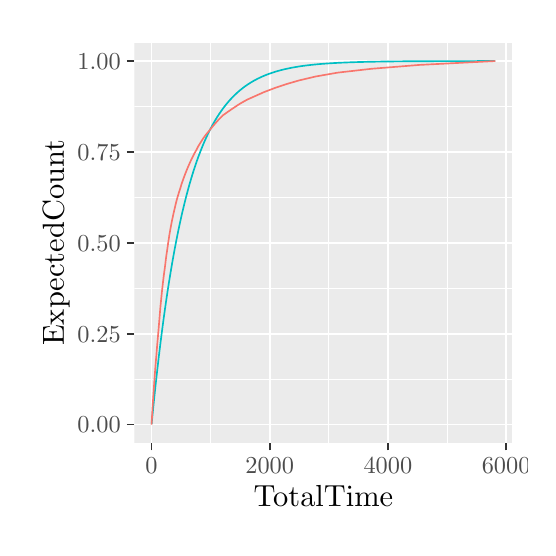
\begin{tikzpicture}[x=1pt,y=1pt]
\definecolor{fillColor}{RGB}{255,255,255}
\path[use as bounding box,fill=fillColor,fill opacity=0.00] (0,0) rectangle (180.67,180.67);
\begin{scope}
\path[clip] (  0.00,  0.00) rectangle (180.67,180.67);
\definecolor{drawColor}{RGB}{255,255,255}
\definecolor{fillColor}{RGB}{255,255,255}

\path[draw=drawColor,line width= 0.6pt,line join=round,line cap=round,fill=fillColor] (  0.00,  0.00) rectangle (180.68,180.68);
\end{scope}
\begin{scope}
\path[clip] ( 38.56, 30.69) rectangle (175.17,175.17);
\definecolor{fillColor}{gray}{0.92}

\path[fill=fillColor] ( 38.56, 30.69) rectangle (175.18,175.17);
\definecolor{drawColor}{RGB}{255,255,255}

\path[draw=drawColor,line width= 0.3pt,line join=round] ( 38.56, 53.67) --
	(175.17, 53.67);

\path[draw=drawColor,line width= 0.3pt,line join=round] ( 38.56, 86.51) --
	(175.17, 86.51);

\path[draw=drawColor,line width= 0.3pt,line join=round] ( 38.56,119.35) --
	(175.17,119.35);

\path[draw=drawColor,line width= 0.3pt,line join=round] ( 38.56,152.19) --
	(175.17,152.19);

\path[draw=drawColor,line width= 0.3pt,line join=round] ( 66.12, 30.69) --
	( 66.12,175.17);

\path[draw=drawColor,line width= 0.3pt,line join=round] (108.82, 30.69) --
	(108.82,175.17);

\path[draw=drawColor,line width= 0.3pt,line join=round] (151.52, 30.69) --
	(151.52,175.17);

\path[draw=drawColor,line width= 0.6pt,line join=round] ( 38.56, 37.25) --
	(175.17, 37.25);

\path[draw=drawColor,line width= 0.6pt,line join=round] ( 38.56, 70.09) --
	(175.17, 70.09);

\path[draw=drawColor,line width= 0.6pt,line join=round] ( 38.56,102.93) --
	(175.17,102.93);

\path[draw=drawColor,line width= 0.6pt,line join=round] ( 38.56,135.77) --
	(175.17,135.77);

\path[draw=drawColor,line width= 0.6pt,line join=round] ( 38.56,168.61) --
	(175.17,168.61);

\path[draw=drawColor,line width= 0.6pt,line join=round] ( 44.77, 30.69) --
	( 44.77,175.17);

\path[draw=drawColor,line width= 0.6pt,line join=round] ( 87.47, 30.69) --
	( 87.47,175.17);

\path[draw=drawColor,line width= 0.6pt,line join=round] (130.17, 30.69) --
	(130.17,175.17);

\path[draw=drawColor,line width= 0.6pt,line join=round] (172.88, 30.69) --
	(172.88,175.17);
\definecolor{drawColor}{RGB}{0,191,196}

\path[draw=drawColor,line width= 0.6pt,line join=round] ( 44.79, 37.47) --
	( 44.81, 37.70) --
	( 44.83, 37.92) --
	( 44.85, 38.14) --
	( 44.87, 38.35) --
	( 44.89, 38.57) --
	( 44.91, 38.79) --
	( 44.94, 39.01) --
	( 44.96, 39.23) --
	( 44.98, 39.45) --
	( 45.00, 39.66) --
	( 45.02, 39.88) --
	( 45.04, 40.10) --
	( 45.06, 40.31) --
	( 45.09, 40.53) --
	( 45.11, 40.75) --
	( 45.13, 40.96) --
	( 45.15, 41.17) --
	( 45.17, 41.39) --
	( 45.19, 41.60) --
	( 45.21, 41.82) --
	( 45.23, 42.03) --
	( 45.26, 42.24) --
	( 45.28, 42.46) --
	( 45.30, 42.67) --
	( 45.32, 42.88) --
	( 45.34, 43.09) --
	( 45.36, 43.30) --
	( 45.38, 43.51) --
	( 45.41, 43.72) --
	( 45.43, 43.93) --
	( 45.45, 44.14) --
	( 45.47, 44.35) --
	( 45.49, 44.56) --
	( 45.51, 44.77) --
	( 45.53, 44.98) --
	( 45.56, 45.19) --
	( 45.58, 45.40) --
	( 45.60, 45.60) --
	( 45.62, 45.81) --
	( 45.64, 46.02) --
	( 45.66, 46.22) --
	( 45.68, 46.43) --
	( 45.70, 46.63) --
	( 45.73, 46.84) --
	( 45.75, 47.04) --
	( 45.77, 47.25) --
	( 45.79, 47.45) --
	( 45.81, 47.66) --
	( 45.83, 47.86) --
	( 45.85, 48.06) --
	( 45.88, 48.27) --
	( 45.90, 48.47) --
	( 45.92, 48.67) --
	( 45.94, 48.87) --
	( 45.96, 49.07) --
	( 45.98, 49.27) --
	( 46.00, 49.48) --
	( 46.02, 49.68) --
	( 46.05, 49.88) --
	( 46.07, 50.08) --
	( 46.09, 50.28) --
	( 46.11, 50.47) --
	( 46.13, 50.67) --
	( 46.15, 50.87) --
	( 46.17, 51.07) --
	( 46.20, 51.27) --
	( 46.22, 51.46) --
	( 46.24, 51.66) --
	( 46.26, 51.86) --
	( 46.28, 52.05) --
	( 46.30, 52.25) --
	( 46.32, 52.45) --
	( 46.35, 52.64) --
	( 46.37, 52.84) --
	( 46.39, 53.03) --
	( 46.41, 53.23) --
	( 46.43, 53.42) --
	( 46.45, 53.61) --
	( 46.47, 53.81) --
	( 46.49, 54.00) --
	( 46.52, 54.19) --
	( 46.54, 54.39) --
	( 46.56, 54.58) --
	( 46.58, 54.77) --
	( 46.60, 54.96) --
	( 46.62, 55.15) --
	( 46.64, 55.34) --
	( 46.67, 55.53) --
	( 46.69, 55.72) --
	( 46.71, 55.91) --
	( 46.73, 56.10) --
	( 46.75, 56.29) --
	( 46.77, 56.48) --
	( 46.79, 56.67) --
	( 46.81, 56.86) --
	( 46.84, 57.05) --
	( 46.86, 57.24) --
	( 46.88, 57.42) --
	( 46.90, 57.61) --
	( 46.92, 57.80) --
	( 46.94, 57.98) --
	( 46.96, 58.17) --
	( 46.99, 58.35) --
	( 47.01, 58.54) --
	( 47.03, 58.73) --
	( 47.05, 58.91) --
	( 47.07, 59.09) --
	( 47.09, 59.28) --
	( 47.11, 59.46) --
	( 47.14, 59.65) --
	( 47.16, 59.83) --
	( 47.18, 60.01) --
	( 47.20, 60.20) --
	( 47.22, 60.38) --
	( 47.24, 60.56) --
	( 47.26, 60.74) --
	( 47.28, 60.92) --
	( 47.31, 61.10) --
	( 47.33, 61.29) --
	( 47.35, 61.47) --
	( 47.37, 61.65) --
	( 47.39, 61.83) --
	( 47.41, 62.01) --
	( 47.43, 62.19) --
	( 47.46, 62.36) --
	( 47.48, 62.54) --
	( 47.50, 62.72) --
	( 47.52, 62.90) --
	( 47.54, 63.08) --
	( 47.56, 63.25) --
	( 47.58, 63.43) --
	( 47.60, 63.61) --
	( 47.63, 63.79) --
	( 47.65, 63.96) --
	( 47.67, 64.14) --
	( 47.69, 64.31) --
	( 47.71, 64.49) --
	( 47.73, 64.66) --
	( 47.75, 64.84) --
	( 47.78, 65.01) --
	( 47.80, 65.19) --
	( 47.82, 65.36) --
	( 47.84, 65.54) --
	( 47.86, 65.71) --
	( 47.88, 65.88) --
	( 47.90, 66.06) --
	( 47.93, 66.23) --
	( 47.95, 66.40) --
	( 47.97, 66.57) --
	( 47.99, 66.74) --
	( 48.01, 66.92) --
	( 48.03, 67.09) --
	( 48.05, 67.26) --
	( 48.07, 67.43) --
	( 48.10, 67.60) --
	( 48.12, 67.77) --
	( 48.14, 67.94) --
	( 48.16, 68.11) --
	( 48.18, 68.28) --
	( 48.20, 68.44) --
	( 48.22, 68.61) --
	( 48.25, 68.78) --
	( 48.27, 68.95) --
	( 48.29, 69.12) --
	( 48.31, 69.28) --
	( 48.33, 69.45) --
	( 48.35, 69.62) --
	( 48.37, 69.78) --
	( 48.39, 69.95) --
	( 48.42, 70.12) --
	( 48.44, 70.28) --
	( 48.46, 70.45) --
	( 48.48, 70.61) --
	( 48.50, 70.78) --
	( 48.52, 70.94) --
	( 48.54, 71.11) --
	( 48.57, 71.27) --
	( 48.59, 71.43) --
	( 48.61, 71.60) --
	( 48.63, 71.76) --
	( 48.65, 71.92) --
	( 48.67, 72.09) --
	( 48.69, 72.25) --
	( 48.72, 72.41) --
	( 48.74, 72.57) --
	( 48.76, 72.74) --
	( 48.78, 72.90) --
	( 48.80, 73.06) --
	( 48.82, 73.22) --
	( 48.84, 73.38) --
	( 48.86, 73.54) --
	( 48.89, 73.70) --
	( 48.91, 73.86) --
	( 48.93, 74.02) --
	( 48.95, 74.18) --
	( 48.97, 74.34) --
	( 48.99, 74.49) --
	( 49.01, 74.65) --
	( 49.04, 74.81) --
	( 49.06, 74.97) --
	( 49.08, 75.13) --
	( 49.10, 75.28) --
	( 49.12, 75.44) --
	( 49.14, 75.60) --
	( 49.16, 75.75) --
	( 49.18, 75.91) --
	( 49.21, 76.07) --
	( 49.23, 76.22) --
	( 49.25, 76.38) --
	( 49.27, 76.53) --
	( 49.29, 76.69) --
	( 49.31, 76.84) --
	( 49.33, 77.00) --
	( 49.36, 77.15) --
	( 49.38, 77.30) --
	( 49.40, 77.46) --
	( 49.42, 77.61) --
	( 49.44, 77.76) --
	( 49.46, 77.92) --
	( 49.48, 78.07) --
	( 49.51, 78.22) --
	( 49.53, 78.37) --
	( 49.55, 78.53) --
	( 49.57, 78.68) --
	( 49.59, 78.83) --
	( 49.61, 78.98) --
	( 49.63, 79.13) --
	( 49.65, 79.28) --
	( 49.68, 79.43) --
	( 49.70, 79.58) --
	( 49.72, 79.73) --
	( 49.74, 79.88) --
	( 49.76, 80.03) --
	( 49.78, 80.18) --
	( 49.80, 80.33) --
	( 49.83, 80.48) --
	( 49.85, 80.62) --
	( 49.87, 80.77) --
	( 49.89, 80.92) --
	( 49.91, 81.07) --
	( 49.93, 81.22) --
	( 49.95, 81.36) --
	( 49.97, 81.51) --
	( 50.00, 81.66) --
	( 50.02, 81.80) --
	( 50.04, 81.95) --
	( 50.06, 82.09) --
	( 50.08, 82.24) --
	( 50.10, 82.38) --
	( 50.12, 82.53) --
	( 50.15, 82.67) --
	( 50.17, 82.82) --
	( 50.19, 82.96) --
	( 50.21, 83.11) --
	( 50.23, 83.25) --
	( 50.25, 83.39) --
	( 50.27, 83.54) --
	( 50.30, 83.68) --
	( 50.32, 83.82) --
	( 50.34, 83.97) --
	( 50.36, 84.11) --
	( 50.38, 84.25) --
	( 50.40, 84.39) --
	( 50.42, 84.54) --
	( 50.44, 84.68) --
	( 50.47, 84.82) --
	( 50.49, 84.96) --
	( 50.51, 85.10) --
	( 50.53, 85.24) --
	( 50.55, 85.38) --
	( 50.57, 85.52) --
	( 50.59, 85.66) --
	( 50.62, 85.80) --
	( 50.64, 85.94) --
	( 50.66, 86.08) --
	( 50.68, 86.22) --
	( 50.70, 86.36) --
	( 50.72, 86.49) --
	( 50.74, 86.63) --
	( 50.76, 86.77) --
	( 50.79, 86.91) --
	( 50.81, 87.04) --
	( 50.83, 87.18) --
	( 50.85, 87.32) --
	( 50.87, 87.46) --
	( 50.89, 87.59) --
	( 50.91, 87.73) --
	( 50.94, 87.86) --
	( 50.96, 88.00) --
	( 50.98, 88.14) --
	( 51.00, 88.27) --
	( 51.02, 88.41) --
	( 51.04, 88.54) --
	( 51.06, 88.68) --
	( 51.09, 88.81) --
	( 51.11, 88.95) --
	( 51.13, 89.08) --
	( 51.15, 89.21) --
	( 51.17, 89.35) --
	( 51.19, 89.48) --
	( 51.21, 89.61) --
	( 51.23, 89.75) --
	( 51.26, 89.88) --
	( 51.28, 90.01) --
	( 51.30, 90.14) --
	( 51.32, 90.28) --
	( 51.34, 90.41) --
	( 51.36, 90.54) --
	( 51.38, 90.67) --
	( 51.41, 90.80) --
	( 51.43, 90.93) --
	( 51.45, 91.06) --
	( 51.47, 91.19) --
	( 51.49, 91.32) --
	( 51.51, 91.45) --
	( 51.53, 91.58) --
	( 51.55, 91.71) --
	( 51.58, 91.84) --
	( 51.60, 91.97) --
	( 51.62, 92.10) --
	( 51.64, 92.23) --
	( 51.66, 92.36) --
	( 51.68, 92.49) --
	( 51.70, 92.61) --
	( 51.73, 92.74) --
	( 51.75, 92.87) --
	( 51.77, 93.00) --
	( 51.79, 93.12) --
	( 51.81, 93.25) --
	( 51.83, 93.38) --
	( 51.85, 93.50) --
	( 51.88, 93.63) --
	( 51.90, 93.76) --
	( 51.92, 93.88) --
	( 51.94, 94.01) --
	( 51.96, 94.13) --
	( 51.98, 94.26) --
	( 52.00, 94.38) --
	( 52.02, 94.51) --
	( 52.05, 94.63) --
	( 52.07, 94.76) --
	( 52.09, 94.88) --
	( 52.11, 95.01) --
	( 52.13, 95.13) --
	( 52.15, 95.25) --
	( 52.17, 95.38) --
	( 52.20, 95.50) --
	( 52.22, 95.62) --
	( 52.24, 95.75) --
	( 52.26, 95.87) --
	( 52.28, 95.99) --
	( 52.30, 96.11) --
	( 52.32, 96.24) --
	( 52.34, 96.36) --
	( 52.37, 96.48) --
	( 52.39, 96.60) --
	( 52.41, 96.72) --
	( 52.43, 96.84) --
	( 52.45, 96.96) --
	( 52.47, 97.08) --
	( 52.49, 97.20) --
	( 52.52, 97.32) --
	( 52.54, 97.44) --
	( 52.56, 97.56) --
	( 52.58, 97.68) --
	( 52.60, 97.80) --
	( 52.62, 97.92) --
	( 52.64, 98.04) --
	( 52.67, 98.16) --
	( 52.69, 98.28) --
	( 52.71, 98.40) --
	( 52.73, 98.51) --
	( 52.75, 98.63) --
	( 52.77, 98.75) --
	( 52.79, 98.87) --
	( 52.81, 98.98) --
	( 52.84, 99.10) --
	( 52.86, 99.22) --
	( 52.88, 99.34) --
	( 52.90, 99.45) --
	( 52.92, 99.57) --
	( 52.94, 99.68) --
	( 52.96, 99.80) --
	( 52.99, 99.92) --
	( 53.01,100.03) --
	( 53.03,100.15) --
	( 53.05,100.26) --
	( 53.07,100.38) --
	( 53.09,100.49) --
	( 53.11,100.61) --
	( 53.13,100.72) --
	( 53.16,100.84) --
	( 53.18,100.95) --
	( 53.20,101.06) --
	( 53.22,101.18) --
	( 53.24,101.29) --
	( 53.26,101.40) --
	( 53.28,101.52) --
	( 53.31,101.63) --
	( 53.33,101.74) --
	( 53.35,101.85) --
	( 53.37,101.97) --
	( 53.39,102.08) --
	( 53.41,102.19) --
	( 53.43,102.30) --
	( 53.46,102.41) --
	( 53.48,102.53) --
	( 53.50,102.64) --
	( 53.52,102.75) --
	( 53.54,102.86) --
	( 53.56,102.97) --
	( 53.58,103.08) --
	( 53.60,103.19) --
	( 53.63,103.30) --
	( 53.65,103.41) --
	( 53.67,103.52) --
	( 53.69,103.63) --
	( 53.71,103.74) --
	( 53.73,103.85) --
	( 53.75,103.96) --
	( 53.78,104.07) --
	( 53.80,104.17) --
	( 53.82,104.28) --
	( 53.84,104.39) --
	( 53.86,104.50) --
	( 53.88,104.61) --
	( 53.90,104.71) --
	( 53.93,104.82) --
	( 53.95,104.93) --
	( 53.97,105.04) --
	( 53.99,105.14) --
	( 54.01,105.25) --
	( 54.03,105.36) --
	( 54.05,105.46) --
	( 54.07,105.57) --
	( 54.10,105.68) --
	( 54.12,105.78) --
	( 54.14,105.89) --
	( 54.16,105.99) --
	( 54.18,106.10) --
	( 54.20,106.20) --
	( 54.22,106.31) --
	( 54.25,106.41) --
	( 54.27,106.52) --
	( 54.29,106.62) --
	( 54.31,106.73) --
	( 54.33,106.83) --
	( 54.35,106.93) --
	( 54.37,107.04) --
	( 54.39,107.14) --
	( 54.42,107.24) --
	( 54.44,107.35) --
	( 54.46,107.45) --
	( 54.48,107.55) --
	( 54.50,107.66) --
	( 54.52,107.76) --
	( 54.54,107.86) --
	( 54.57,107.96) --
	( 54.59,108.07) --
	( 54.61,108.17) --
	( 54.63,108.27) --
	( 54.65,108.37) --
	( 54.67,108.47) --
	( 54.69,108.57) --
	( 54.72,108.67) --
	( 54.74,108.78) --
	( 54.76,108.88) --
	( 54.78,108.98) --
	( 54.80,109.08) --
	( 54.82,109.18) --
	( 54.84,109.28) --
	( 54.86,109.38) --
	( 54.89,109.48) --
	( 54.91,109.58) --
	( 54.93,109.68) --
	( 54.95,109.77) --
	( 54.97,109.87) --
	( 54.99,109.97) --
	( 55.01,110.07) --
	( 55.04,110.17) --
	( 55.06,110.27) --
	( 55.08,110.37) --
	( 55.10,110.46) --
	( 55.12,110.56) --
	( 55.14,110.66) --
	( 55.16,110.76) --
	( 55.18,110.85) --
	( 55.21,110.95) --
	( 55.23,111.05) --
	( 55.25,111.14) --
	( 55.27,111.24) --
	( 55.29,111.34) --
	( 55.31,111.43) --
	( 55.33,111.53) --
	( 55.36,111.63) --
	( 55.38,111.72) --
	( 55.40,111.82) --
	( 55.42,111.91) --
	( 55.44,112.01) --
	( 55.46,112.10) --
	( 55.48,112.20) --
	( 55.51,112.29) --
	( 55.53,112.39) --
	( 55.55,112.48) --
	( 55.57,112.58) --
	( 55.59,112.67) --
	( 55.61,112.77) --
	( 55.63,112.86) --
	( 55.65,112.95) --
	( 55.68,113.05) --
	( 55.70,113.14) --
	( 55.72,113.23) --
	( 55.74,113.33) --
	( 55.76,113.42) --
	( 55.78,113.51) --
	( 55.80,113.61) --
	( 55.83,113.70) --
	( 55.85,113.79) --
	( 55.87,113.88) --
	( 55.89,113.98) --
	( 55.91,114.07) --
	( 55.93,114.16) --
	( 55.95,114.25) --
	( 55.97,114.34) --
	( 56.00,114.43) --
	( 56.02,114.52) --
	( 56.04,114.62) --
	( 56.06,114.71) --
	( 56.08,114.80) --
	( 56.10,114.89) --
	( 56.12,114.98) --
	( 56.15,115.07) --
	( 56.17,115.16) --
	( 56.19,115.25) --
	( 56.21,115.34) --
	( 56.23,115.43) --
	( 56.25,115.52) --
	( 56.27,115.61) --
	( 56.30,115.70) --
	( 56.32,115.78) --
	( 56.34,115.87) --
	( 56.36,115.96) --
	( 56.38,116.05) --
	( 56.40,116.14) --
	( 56.42,116.23) --
	( 56.44,116.32) --
	( 56.47,116.40) --
	( 56.49,116.49) --
	( 56.51,116.58) --
	( 56.53,116.67) --
	( 56.55,116.75) --
	( 56.57,116.84) --
	( 56.59,116.93) --
	( 56.62,117.02) --
	( 56.64,117.10) --
	( 56.66,117.19) --
	( 56.68,117.28) --
	( 56.70,117.36) --
	( 56.72,117.45) --
	( 56.74,117.53) --
	( 56.76,117.62) --
	( 56.79,117.71) --
	( 56.81,117.79) --
	( 56.83,117.88) --
	( 56.85,117.96) --
	( 56.87,118.05) --
	( 56.89,118.13) --
	( 56.91,118.22) --
	( 56.94,118.30) --
	( 56.96,118.39) --
	( 56.98,118.47) --
	( 57.00,118.56) --
	( 57.02,118.64) --
	( 57.04,118.72) --
	( 57.06,118.81) --
	( 57.09,118.89) --
	( 57.11,118.98) --
	( 57.13,119.06) --
	( 57.15,119.14) --
	( 57.17,119.23) --
	( 57.19,119.31) --
	( 57.21,119.39) --
	( 57.23,119.47) --
	( 57.26,119.56) --
	( 57.28,119.64) --
	( 57.30,119.72) --
	( 57.32,119.80) --
	( 57.34,119.89) --
	( 57.36,119.97) --
	( 57.38,120.05) --
	( 57.41,120.13) --
	( 57.43,120.21) --
	( 57.45,120.29) --
	( 57.47,120.38) --
	( 57.49,120.46) --
	( 57.51,120.54) --
	( 57.53,120.62) --
	( 57.55,120.70) --
	( 57.58,120.78) --
	( 57.60,120.86) --
	( 57.62,120.94) --
	( 57.64,121.02) --
	( 57.66,121.10) --
	( 57.68,121.18) --
	( 57.70,121.26) --
	( 57.73,121.34) --
	( 57.75,121.42) --
	( 57.77,121.50) --
	( 57.79,121.58) --
	( 57.81,121.66) --
	( 57.83,121.74) --
	( 57.85,121.82) --
	( 57.88,121.89) --
	( 57.90,121.97) --
	( 57.92,122.05) --
	( 57.94,122.13) --
	( 57.96,122.21) --
	( 57.98,122.29) --
	( 58.00,122.36) --
	( 58.02,122.44) --
	( 58.05,122.52) --
	( 58.07,122.60) --
	( 58.09,122.67) --
	( 58.11,122.75) --
	( 58.13,122.83) --
	( 58.15,122.91) --
	( 58.17,122.98) --
	( 58.20,123.06) --
	( 58.22,123.14) --
	( 58.24,123.21) --
	( 58.26,123.29) --
	( 58.28,123.37) --
	( 58.30,123.44) --
	( 58.32,123.52) --
	( 58.34,123.59) --
	( 58.37,123.67) --
	( 58.39,123.74) --
	( 58.41,123.82) --
	( 58.43,123.90) --
	( 58.45,123.97) --
	( 58.47,124.05) --
	( 58.49,124.12) --
	( 58.52,124.20) --
	( 58.54,124.27) --
	( 58.56,124.34) --
	( 58.58,124.42) --
	( 58.60,124.49) --
	( 58.62,124.57) --
	( 58.64,124.64) --
	( 58.67,124.72) --
	( 58.69,124.79) --
	( 58.71,124.86) --
	( 58.73,124.94) --
	( 58.75,125.01) --
	( 58.77,125.08) --
	( 58.79,125.16) --
	( 58.81,125.23) --
	( 58.84,125.30) --
	( 58.86,125.38) --
	( 58.88,125.45) --
	( 58.90,125.52) --
	( 58.92,125.59) --
	( 58.94,125.67) --
	( 58.96,125.74) --
	( 58.99,125.81) --
	( 59.01,125.88) --
	( 59.03,125.95) --
	( 59.05,126.03) --
	( 59.07,126.10) --
	( 59.09,126.17) --
	( 59.11,126.24) --
	( 59.13,126.31) --
	( 59.16,126.38) --
	( 59.18,126.45) --
	( 59.20,126.53) --
	( 59.22,126.60) --
	( 59.24,126.67) --
	( 59.26,126.74) --
	( 59.28,126.81) --
	( 59.31,126.88) --
	( 59.33,126.95) --
	( 59.35,127.02) --
	( 59.37,127.09) --
	( 59.39,127.16) --
	( 59.41,127.23) --
	( 59.43,127.30) --
	( 59.46,127.37) --
	( 59.48,127.44) --
	( 59.50,127.51) --
	( 59.52,127.57) --
	( 59.54,127.64) --
	( 59.56,127.71) --
	( 59.58,127.78) --
	( 59.60,127.85) --
	( 59.63,127.92) --
	( 59.65,127.99) --
	( 59.67,128.06) --
	( 59.69,128.12) --
	( 59.71,128.19) --
	( 59.73,128.26) --
	( 59.75,128.33) --
	( 59.78,128.40) --
	( 59.80,128.46) --
	( 59.82,128.53) --
	( 59.84,128.60) --
	( 59.86,128.67) --
	( 59.88,128.73) --
	( 59.90,128.80) --
	( 59.92,128.87) --
	( 59.95,128.93) --
	( 59.97,129.00) --
	( 59.99,129.07) --
	( 60.01,129.13) --
	( 60.03,129.20) --
	( 60.05,129.27) --
	( 60.07,129.33) --
	( 60.10,129.40) --
	( 60.12,129.46) --
	( 60.14,129.53) --
	( 60.16,129.60) --
	( 60.18,129.66) --
	( 60.20,129.73) --
	( 60.22,129.79) --
	( 60.25,129.86) --
	( 60.27,129.92) --
	( 60.29,129.99) --
	( 60.31,130.05) --
	( 60.33,130.12) --
	( 60.35,130.18) --
	( 60.37,130.25) --
	( 60.39,130.31) --
	( 60.42,130.38) --
	( 60.44,130.44) --
	( 60.46,130.51) --
	( 60.48,130.57) --
	( 60.50,130.63) --
	( 60.52,130.70) --
	( 60.54,130.76) --
	( 60.57,130.82) --
	( 60.59,130.89) --
	( 60.61,130.95) --
	( 60.63,131.01) --
	( 60.65,131.08) --
	( 60.67,131.14) --
	( 60.69,131.20) --
	( 60.71,131.27) --
	( 60.74,131.33) --
	( 60.76,131.39) --
	( 60.78,131.46) --
	( 60.80,131.52) --
	( 60.82,131.58) --
	( 60.84,131.64) --
	( 60.86,131.70) --
	( 60.89,131.77) --
	( 60.91,131.83) --
	( 60.93,131.89) --
	( 60.95,131.95) --
	( 60.97,132.01) --
	( 60.99,132.08) --
	( 61.01,132.14) --
	( 61.04,132.20) --
	( 61.06,132.26) --
	( 61.08,132.32) --
	( 61.10,132.38) --
	( 61.12,132.44) --
	( 61.14,132.50) --
	( 61.16,132.56) --
	( 61.18,132.63) --
	( 61.21,132.69) --
	( 61.23,132.75) --
	( 61.25,132.81) --
	( 61.27,132.87) --
	( 61.29,132.93) --
	( 61.31,132.99) --
	( 61.33,133.05) --
	( 61.36,133.11) --
	( 61.38,133.17) --
	( 61.40,133.23) --
	( 61.42,133.29) --
	( 61.44,133.34) --
	( 61.46,133.40) --
	( 61.48,133.46) --
	( 61.50,133.52) --
	( 61.53,133.58) --
	( 61.55,133.64) --
	( 61.57,133.70) --
	( 61.59,133.76) --
	( 61.61,133.82) --
	( 61.63,133.88) --
	( 61.65,133.93) --
	( 61.68,133.99) --
	( 61.70,134.05) --
	( 61.72,134.11) --
	( 61.74,134.17) --
	( 61.76,134.22) --
	( 61.78,134.28) --
	( 61.80,134.34) --
	( 61.83,134.40) --
	( 61.85,134.46) --
	( 61.87,134.51) --
	( 61.89,134.57) --
	( 61.91,134.63) --
	( 61.93,134.68) --
	( 61.95,134.74) --
	( 61.97,134.80) --
	( 62.00,134.86) --
	( 62.02,134.91) --
	( 62.04,134.97) --
	( 62.06,135.03) --
	( 62.08,135.08) --
	( 62.10,135.14) --
	( 62.12,135.19) --
	( 62.15,135.25) --
	( 62.17,135.31) --
	( 62.19,135.36) --
	( 62.21,135.42) --
	( 62.23,135.47) --
	( 62.25,135.53) --
	( 62.27,135.59) --
	( 62.29,135.64) --
	( 62.32,135.70) --
	( 62.34,135.75) --
	( 62.36,135.81) --
	( 62.38,135.86) --
	( 62.40,135.92) --
	( 62.42,135.97) --
	( 62.44,136.03) --
	( 62.47,136.08) --
	( 62.49,136.14) --
	( 62.51,136.19) --
	( 62.53,136.25) --
	( 62.55,136.30) --
	( 62.57,136.36) --
	( 62.59,136.41) --
	( 62.62,136.46) --
	( 62.64,136.52) --
	( 62.66,136.57) --
	( 62.68,136.63) --
	( 62.70,136.68) --
	( 62.72,136.73) --
	( 62.74,136.79) --
	( 62.76,136.84) --
	( 62.79,136.89) --
	( 62.81,136.95) --
	( 62.83,137.00) --
	( 62.85,137.05) --
	( 62.87,137.11) --
	( 62.89,137.16) --
	( 62.91,137.21) --
	( 62.94,137.27) --
	( 62.96,137.32) --
	( 62.98,137.37) --
	( 63.00,137.42) --
	( 63.02,137.48) --
	( 63.04,137.53) --
	( 63.06,137.58) --
	( 63.08,137.63) --
	( 63.11,137.69) --
	( 63.13,137.74) --
	( 63.15,137.79) --
	( 63.17,137.84) --
	( 63.19,137.89) --
	( 63.21,137.94) --
	( 63.23,138.00) --
	( 63.26,138.05) --
	( 63.28,138.10) --
	( 63.30,138.15) --
	( 63.32,138.20) --
	( 63.34,138.25) --
	( 63.36,138.30) --
	( 63.38,138.35) --
	( 63.41,138.41) --
	( 63.43,138.46) --
	( 63.45,138.51) --
	( 63.47,138.56) --
	( 63.49,138.61) --
	( 63.51,138.66) --
	( 63.53,138.71) --
	( 63.55,138.76) --
	( 63.58,138.81) --
	( 63.60,138.86) --
	( 63.62,138.91) --
	( 63.64,138.96) --
	( 63.66,139.01) --
	( 63.68,139.06) --
	( 63.70,139.11) --
	( 63.73,139.16) --
	( 63.75,139.21) --
	( 63.77,139.26) --
	( 63.79,139.31) --
	( 63.81,139.36) --
	( 63.83,139.41) --
	( 63.85,139.45) --
	( 63.88,139.50) --
	( 63.90,139.55) --
	( 63.92,139.60) --
	( 63.94,139.65) --
	( 63.96,139.70) --
	( 63.98,139.75) --
	( 64.00,139.80) --
	( 64.02,139.84) --
	( 64.05,139.89) --
	( 64.07,139.94) --
	( 64.09,139.99) --
	( 64.11,140.04) --
	( 64.13,140.09) --
	( 64.15,140.13) --
	( 64.17,140.18) --
	( 64.20,140.23) --
	( 64.22,140.28) --
	( 64.24,140.33) --
	( 64.26,140.37) --
	( 64.28,140.42) --
	( 64.30,140.47) --
	( 64.32,140.51) --
	( 64.34,140.56) --
	( 64.37,140.61) --
	( 64.39,140.66) --
	( 64.41,140.70) --
	( 64.43,140.75) --
	( 64.45,140.80) --
	( 64.47,140.84) --
	( 64.49,140.89) --
	( 64.52,140.94) --
	( 64.54,140.98) --
	( 64.56,141.03) --
	( 64.58,141.08) --
	( 64.60,141.12) --
	( 64.62,141.17) --
	( 64.64,141.22) --
	( 64.67,141.26) --
	( 64.69,141.31) --
	( 64.71,141.35) --
	( 64.73,141.40) --
	( 64.75,141.45) --
	( 64.77,141.49) --
	( 64.79,141.54) --
	( 64.81,141.58) --
	( 64.84,141.63) --
	( 64.86,141.67) --
	( 64.88,141.72) --
	( 64.90,141.76) --
	( 64.92,141.81) --
	( 64.94,141.85) --
	( 64.96,141.90) --
	( 64.99,141.94) --
	( 65.01,141.99) --
	( 65.03,142.03) --
	( 65.05,142.08) --
	( 65.07,142.12) --
	( 65.09,142.17) --
	( 65.11,142.21) --
	( 65.13,142.26) --
	( 65.16,142.30) --
	( 65.18,142.34) --
	( 65.20,142.39) --
	( 65.22,142.43) --
	( 65.24,142.48) --
	( 65.26,142.52) --
	( 65.28,142.56) --
	( 65.31,142.61) --
	( 65.33,142.65) --
	( 65.35,142.70) --
	( 65.37,142.74) --
	( 65.39,142.78) --
	( 65.41,142.83) --
	( 65.43,142.87) --
	( 65.46,142.91) --
	( 65.48,142.96) --
	( 65.50,143.00) --
	( 65.52,143.04) --
	( 65.54,143.09) --
	( 65.56,143.13) --
	( 65.58,143.17) --
	( 65.60,143.21) --
	( 65.63,143.26) --
	( 65.65,143.30) --
	( 65.67,143.34) --
	( 65.69,143.38) --
	( 65.71,143.43) --
	( 65.73,143.47) --
	( 65.75,143.51) --
	( 65.78,143.55) --
	( 65.80,143.60) --
	( 65.82,143.64) --
	( 65.84,143.68) --
	( 65.86,143.72) --
	( 65.88,143.76) --
	( 65.90,143.81) --
	( 65.92,143.85) --
	( 65.95,143.89) --
	( 65.97,143.93) --
	( 65.99,143.97) --
	( 66.01,144.01) --
	( 66.03,144.06) --
	( 66.05,144.10) --
	( 66.07,144.14) --
	( 66.10,144.18) --
	( 66.12,144.22) --
	( 66.14,144.26) --
	( 66.16,144.30) --
	( 66.18,144.34) --
	( 66.20,144.38) --
	( 66.22,144.42) --
	( 66.25,144.47) --
	( 66.27,144.51) --
	( 66.29,144.55) --
	( 66.31,144.59) --
	( 66.33,144.63) --
	( 66.35,144.67) --
	( 66.37,144.71) --
	( 66.39,144.75) --
	( 66.42,144.79) --
	( 66.44,144.83) --
	( 66.46,144.87) --
	( 66.48,144.91) --
	( 66.50,144.95) --
	( 66.52,144.99) --
	( 66.54,145.03) --
	( 66.57,145.07) --
	( 66.59,145.11) --
	( 66.61,145.15) --
	( 66.63,145.19) --
	( 66.65,145.23) --
	( 66.67,145.26) --
	( 66.69,145.30) --
	( 66.71,145.34) --
	( 66.74,145.38) --
	( 66.76,145.42) --
	( 66.78,145.46) --
	( 66.80,145.50) --
	( 66.82,145.54) --
	( 66.84,145.58) --
	( 66.86,145.62) --
	( 66.89,145.65) --
	( 66.91,145.69) --
	( 66.93,145.73) --
	( 66.95,145.77) --
	( 66.97,145.81) --
	( 66.99,145.85) --
	( 67.01,145.89) --
	( 67.04,145.92) --
	( 67.06,145.96) --
	( 67.08,146.00) --
	( 67.10,146.04) --
	( 67.12,146.08) --
	( 67.14,146.11) --
	( 67.16,146.15) --
	( 67.18,146.19) --
	( 67.21,146.23) --
	( 67.23,146.26) --
	( 67.25,146.30) --
	( 67.27,146.34) --
	( 67.29,146.38) --
	( 67.31,146.41) --
	( 67.33,146.45) --
	( 67.36,146.49) --
	( 67.38,146.53) --
	( 67.40,146.56) --
	( 67.42,146.60) --
	( 67.44,146.64) --
	( 67.46,146.67) --
	( 67.48,146.71) --
	( 67.50,146.75) --
	( 67.53,146.79) --
	( 67.55,146.82) --
	( 67.57,146.86) --
	( 67.59,146.90) --
	( 67.61,146.93) --
	( 67.63,146.97) --
	( 67.65,147.00) --
	( 67.68,147.04) --
	( 67.70,147.08) --
	( 67.72,147.11) --
	( 67.74,147.15) --
	( 67.76,147.19) --
	( 67.78,147.22) --
	( 67.80,147.26) --
	( 67.83,147.29) --
	( 67.85,147.33) --
	( 67.87,147.37) --
	( 67.89,147.40) --
	( 67.91,147.44) --
	( 67.93,147.47) --
	( 67.95,147.51) --
	( 67.97,147.54) --
	( 68.00,147.58) --
	( 68.02,147.61) --
	( 68.04,147.65) --
	( 68.06,147.68) --
	( 68.08,147.72) --
	( 68.10,147.76) --
	( 68.12,147.79) --
	( 68.15,147.83) --
	( 68.17,147.86) --
	( 68.19,147.90) --
	( 68.21,147.93) --
	( 68.23,147.96) --
	( 68.25,148.00) --
	( 68.27,148.03) --
	( 68.29,148.07) --
	( 68.32,148.10) --
	( 68.34,148.14) --
	( 68.36,148.17) --
	( 68.38,148.21) --
	( 68.40,148.24) --
	( 68.42,148.28) --
	( 68.44,148.31) --
	( 68.47,148.34) --
	( 68.49,148.38) --
	( 68.51,148.41) --
	( 68.53,148.45) --
	( 68.55,148.48) --
	( 68.57,148.51) --
	( 68.59,148.55) --
	( 68.62,148.58) --
	( 68.64,148.61) --
	( 68.66,148.65) --
	( 68.68,148.68) --
	( 68.70,148.72) --
	( 68.72,148.75) --
	( 68.74,148.78) --
	( 68.76,148.82) --
	( 68.79,148.85) --
	( 68.81,148.88) --
	( 68.83,148.92) --
	( 68.85,148.95) --
	( 68.87,148.98) --
	( 68.89,149.01) --
	( 68.91,149.05) --
	( 68.94,149.08) --
	( 68.96,149.11) --
	( 68.98,149.15) --
	( 69.00,149.18) --
	( 69.02,149.21) --
	( 69.04,149.24) --
	( 69.06,149.28) --
	( 69.08,149.31) --
	( 69.11,149.34) --
	( 69.13,149.37) --
	( 69.15,149.41) --
	( 69.17,149.44) --
	( 69.19,149.47) --
	( 69.21,149.50) --
	( 69.23,149.54) --
	( 69.26,149.57) --
	( 69.28,149.60) --
	( 69.30,149.63) --
	( 69.32,149.66) --
	( 69.34,149.70) --
	( 69.36,149.73) --
	( 69.38,149.76) --
	( 69.41,149.79) --
	( 69.43,149.82) --
	( 69.45,149.85) --
	( 69.47,149.89) --
	( 69.49,149.92) --
	( 69.51,149.95) --
	( 69.53,149.98) --
	( 69.55,150.01) --
	( 69.58,150.04) --
	( 69.60,150.07) --
	( 69.62,150.10) --
	( 69.64,150.14) --
	( 69.66,150.17) --
	( 69.68,150.20) --
	( 69.70,150.23) --
	( 69.73,150.26) --
	( 69.75,150.29) --
	( 69.77,150.32) --
	( 69.79,150.35) --
	( 69.81,150.38) --
	( 69.83,150.41) --
	( 69.85,150.44) --
	( 69.87,150.47) --
	( 69.90,150.51) --
	( 69.92,150.54) --
	( 69.94,150.57) --
	( 69.96,150.60) --
	( 69.98,150.63) --
	( 70.00,150.66) --
	( 70.02,150.69) --
	( 70.05,150.72) --
	( 70.07,150.75) --
	( 70.09,150.78) --
	( 70.11,150.81) --
	( 70.13,150.84) --
	( 70.15,150.87) --
	( 70.17,150.90) --
	( 70.20,150.93) --
	( 70.22,150.96) --
	( 70.24,150.99) --
	( 70.26,151.02) --
	( 70.28,151.05) --
	( 70.30,151.08) --
	( 70.32,151.10) --
	( 70.34,151.13) --
	( 70.37,151.16) --
	( 70.39,151.19) --
	( 70.41,151.22) --
	( 70.43,151.25) --
	( 70.45,151.28) --
	( 70.47,151.31) --
	( 70.49,151.34) --
	( 70.52,151.37) --
	( 70.54,151.40) --
	( 70.56,151.43) --
	( 70.58,151.45) --
	( 70.60,151.48) --
	( 70.62,151.51) --
	( 70.64,151.54) --
	( 70.66,151.57) --
	( 70.69,151.60) --
	( 70.71,151.63) --
	( 70.73,151.66) --
	( 70.75,151.68) --
	( 70.77,151.71) --
	( 70.79,151.74) --
	( 70.81,151.77) --
	( 70.84,151.80) --
	( 70.86,151.83) --
	( 70.88,151.85) --
	( 70.90,151.88) --
	( 70.92,151.91) --
	( 70.94,151.94) --
	( 70.96,151.97) --
	( 70.99,152.00) --
	( 71.01,152.02) --
	( 71.03,152.05) --
	( 71.05,152.08) --
	( 71.07,152.11) --
	( 71.09,152.13) --
	( 71.11,152.16) --
	( 71.13,152.19) --
	( 71.16,152.22) --
	( 71.18,152.24) --
	( 71.20,152.27) --
	( 71.22,152.30) --
	( 71.24,152.33) --
	( 71.26,152.35) --
	( 71.28,152.38) --
	( 71.31,152.41) --
	( 71.33,152.44) --
	( 71.35,152.46) --
	( 71.37,152.49) --
	( 71.39,152.52) --
	( 71.41,152.55) --
	( 71.43,152.57) --
	( 71.45,152.60) --
	( 71.48,152.63) --
	( 71.50,152.65) --
	( 71.52,152.68) --
	( 71.54,152.71) --
	( 71.56,152.73) --
	( 71.58,152.76) --
	( 71.60,152.79) --
	( 71.63,152.81) --
	( 71.65,152.84) --
	( 71.67,152.87) --
	( 71.69,152.89) --
	( 71.71,152.92) --
	( 71.73,152.95) --
	( 71.75,152.97) --
	( 71.78,153.00) --
	( 71.80,153.02) --
	( 71.82,153.05) --
	( 71.84,153.08) --
	( 71.86,153.10) --
	( 71.88,153.13) --
	( 71.90,153.16) --
	( 71.92,153.18) --
	( 71.95,153.21) --
	( 71.97,153.23) --
	( 71.99,153.26) --
	( 72.01,153.28) --
	( 72.03,153.31) --
	( 72.05,153.34) --
	( 72.07,153.36) --
	( 72.10,153.39) --
	( 72.12,153.41) --
	( 72.14,153.44) --
	( 72.16,153.46) --
	( 72.18,153.49) --
	( 72.20,153.52) --
	( 72.22,153.54) --
	( 72.24,153.57) --
	( 72.27,153.59) --
	( 72.29,153.62) --
	( 72.31,153.64) --
	( 72.33,153.67) --
	( 72.35,153.69) --
	( 72.37,153.72) --
	( 72.39,153.74) --
	( 72.42,153.77) --
	( 72.44,153.79) --
	( 72.46,153.82) --
	( 72.48,153.84) --
	( 72.50,153.87) --
	( 72.52,153.89) --
	( 72.54,153.92) --
	( 72.57,153.94) --
	( 72.59,153.97) --
	( 72.61,153.99) --
	( 72.63,154.02) --
	( 72.65,154.04) --
	( 72.67,154.06) --
	( 72.69,154.09) --
	( 72.71,154.11) --
	( 72.74,154.14) --
	( 72.76,154.16) --
	( 72.78,154.19) --
	( 72.80,154.21) --
	( 72.82,154.23) --
	( 72.84,154.26) --
	( 72.86,154.28) --
	( 72.89,154.31) --
	( 72.91,154.33) --
	( 72.93,154.36) --
	( 72.95,154.38) --
	( 72.97,154.40) --
	( 72.99,154.43) --
	( 73.01,154.45) --
	( 73.03,154.47) --
	( 73.06,154.50) --
	( 73.08,154.52) --
	( 73.10,154.55) --
	( 73.12,154.57) --
	( 73.14,154.59) --
	( 73.16,154.62) --
	( 73.18,154.64) --
	( 73.21,154.66) --
	( 73.23,154.69) --
	( 73.25,154.71) --
	( 73.27,154.73) --
	( 73.29,154.76) --
	( 73.31,154.78) --
	( 73.33,154.80) --
	( 73.36,154.83) --
	( 73.38,154.85) --
	( 73.40,154.87) --
	( 73.42,154.90) --
	( 73.44,154.92) --
	( 73.46,154.94) --
	( 73.48,154.97) --
	( 73.50,154.99) --
	( 73.53,155.01) --
	( 73.55,155.03) --
	( 73.57,155.06) --
	( 73.59,155.08) --
	( 73.61,155.10) --
	( 73.63,155.13) --
	( 73.65,155.15) --
	( 73.68,155.17) --
	( 73.70,155.19) --
	( 73.72,155.22) --
	( 73.74,155.24) --
	( 73.76,155.26) --
	( 73.78,155.28) --
	( 73.80,155.31) --
	( 73.83,155.33) --
	( 73.85,155.35) --
	( 73.87,155.37) --
	( 73.89,155.40) --
	( 73.91,155.42) --
	( 73.93,155.44) --
	( 73.95,155.46) --
	( 73.97,155.48) --
	( 74.00,155.51) --
	( 74.02,155.53) --
	( 74.04,155.55) --
	( 74.06,155.57) --
	( 74.08,155.59) --
	( 74.10,155.62) --
	( 74.12,155.64) --
	( 74.15,155.66) --
	( 74.17,155.68) --
	( 74.19,155.70) --
	( 74.21,155.72) --
	( 74.23,155.75) --
	( 74.25,155.77) --
	( 74.27,155.79) --
	( 74.29,155.81) --
	( 74.32,155.83) --
	( 74.34,155.85) --
	( 74.36,155.88) --
	( 74.38,155.90) --
	( 74.40,155.92) --
	( 74.42,155.94) --
	( 74.44,155.96) --
	( 74.47,155.98) --
	( 74.49,156.00) --
	( 74.51,156.02) --
	( 74.53,156.05) --
	( 74.55,156.07) --
	( 74.57,156.09) --
	( 74.59,156.11) --
	( 74.62,156.13) --
	( 74.64,156.15) --
	( 74.66,156.17) --
	( 74.68,156.19) --
	( 74.70,156.21) --
	( 74.72,156.23) --
	( 74.74,156.26) --
	( 74.76,156.28) --
	( 74.79,156.30) --
	( 74.81,156.32) --
	( 74.83,156.34) --
	( 74.85,156.36) --
	( 74.87,156.38) --
	( 74.89,156.40) --
	( 74.91,156.42) --
	( 74.94,156.44) --
	( 74.96,156.46) --
	( 74.98,156.48) --
	( 75.00,156.50) --
	( 75.02,156.52) --
	( 75.04,156.54) --
	( 75.06,156.56) --
	( 75.08,156.58) --
	( 75.11,156.60) --
	( 75.13,156.62) --
	( 75.15,156.64) --
	( 75.17,156.66) --
	( 75.19,156.68) --
	( 75.21,156.70) --
	( 75.23,156.72) --
	( 75.26,156.74) --
	( 75.28,156.76) --
	( 75.30,156.78) --
	( 75.32,156.80) --
	( 75.34,156.82) --
	( 75.36,156.84) --
	( 75.38,156.86) --
	( 75.41,156.88) --
	( 75.43,156.90) --
	( 75.45,156.92) --
	( 75.47,156.94) --
	( 75.49,156.96) --
	( 75.51,156.98) --
	( 75.53,157.00) --
	( 75.55,157.02) --
	( 75.58,157.04) --
	( 75.60,157.06) --
	( 75.62,157.08) --
	( 75.64,157.10) --
	( 75.66,157.12) --
	( 75.68,157.14) --
	( 75.70,157.16) --
	( 75.73,157.18) --
	( 75.75,157.20) --
	( 75.77,157.21) --
	( 75.79,157.23) --
	( 75.81,157.25) --
	( 75.83,157.27) --
	( 75.85,157.29) --
	( 75.87,157.31) --
	( 75.90,157.33) --
	( 75.92,157.35) --
	( 75.94,157.37) --
	( 75.96,157.39) --
	( 75.98,157.40) --
	( 76.00,157.42) --
	( 76.02,157.44) --
	( 76.05,157.46) --
	( 76.07,157.48) --
	( 76.09,157.50) --
	( 76.11,157.52) --
	( 76.13,157.54) --
	( 76.15,157.55) --
	( 76.17,157.57) --
	( 76.20,157.59) --
	( 76.22,157.61) --
	( 76.24,157.63) --
	( 76.26,157.65) --
	( 76.28,157.67) --
	( 76.30,157.68) --
	( 76.32,157.70) --
	( 76.34,157.72) --
	( 76.37,157.74) --
	( 76.39,157.76) --
	( 76.41,157.78) --
	( 76.43,157.79) --
	( 76.45,157.81) --
	( 76.47,157.83) --
	( 76.49,157.85) --
	( 76.52,157.87) --
	( 76.54,157.88) --
	( 76.56,157.90) --
	( 76.58,157.92) --
	( 76.60,157.94) --
	( 76.62,157.96) --
	( 76.64,157.97) --
	( 76.66,157.99) --
	( 76.69,158.01) --
	( 76.71,158.03) --
	( 76.73,158.05) --
	( 76.75,158.06) --
	( 76.77,158.08) --
	( 76.79,158.10) --
	( 76.81,158.12) --
	( 76.84,158.13) --
	( 76.86,158.15) --
	( 76.88,158.17) --
	( 76.90,158.19) --
	( 76.92,158.20) --
	( 76.94,158.22) --
	( 76.96,158.24) --
	( 76.99,158.26) --
	( 77.01,158.27) --
	( 77.03,158.29) --
	( 77.05,158.31) --
	( 77.07,158.33) --
	( 77.09,158.34) --
	( 77.11,158.36) --
	( 77.13,158.38) --
	( 77.16,158.40) --
	( 77.18,158.41) --
	( 77.20,158.43) --
	( 77.22,158.45) --
	( 77.24,158.46) --
	( 77.26,158.48) --
	( 77.28,158.50) --
	( 77.31,158.52) --
	( 77.33,158.53) --
	( 77.35,158.55) --
	( 77.37,158.57) --
	( 77.39,158.58) --
	( 77.41,158.60) --
	( 77.43,158.62) --
	( 77.45,158.63) --
	( 77.48,158.65) --
	( 77.50,158.67) --
	( 77.52,158.68) --
	( 77.54,158.70) --
	( 77.56,158.72) --
	( 77.58,158.73) --
	( 77.60,158.75) --
	( 77.63,158.77) --
	( 77.65,158.78) --
	( 77.67,158.80) --
	( 77.69,158.82) --
	( 77.71,158.83) --
	( 77.73,158.85) --
	( 77.75,158.87) --
	( 77.78,158.88) --
	( 77.80,158.90) --
	( 77.82,158.92) --
	( 77.84,158.93) --
	( 77.86,158.95) --
	( 77.88,158.96) --
	( 77.90,158.98) --
	( 77.92,159.00) --
	( 77.95,159.01) --
	( 77.97,159.03) --
	( 77.99,159.04) --
	( 78.01,159.06) --
	( 78.03,159.08) --
	( 78.05,159.09) --
	( 78.07,159.11) --
	( 78.10,159.13) --
	( 78.12,159.14) --
	( 78.14,159.16) --
	( 78.16,159.17) --
	( 78.18,159.19) --
	( 78.20,159.20) --
	( 78.22,159.22) --
	( 78.24,159.24) --
	( 78.27,159.25) --
	( 78.29,159.27) --
	( 78.31,159.28) --
	( 78.33,159.30) --
	( 78.35,159.31) --
	( 78.37,159.33) --
	( 78.39,159.35) --
	( 78.42,159.36) --
	( 78.44,159.38) --
	( 78.46,159.39) --
	( 78.48,159.41) --
	( 78.50,159.42) --
	( 78.52,159.44) --
	( 78.54,159.45) --
	( 78.57,159.47) --
	( 78.59,159.49) --
	( 78.61,159.50) --
	( 78.63,159.52) --
	( 78.65,159.53) --
	( 78.67,159.55) --
	( 78.69,159.56) --
	( 78.71,159.58) --
	( 78.74,159.59) --
	( 78.76,159.61) --
	( 78.78,159.62) --
	( 78.80,159.64) --
	( 78.82,159.65) --
	( 78.84,159.67) --
	( 78.86,159.68) --
	( 78.89,159.70) --
	( 78.91,159.71) --
	( 78.93,159.73) --
	( 78.95,159.74) --
	( 78.97,159.76) --
	( 78.99,159.77) --
	( 79.01,159.79) --
	( 79.03,159.80) --
	( 79.06,159.82) --
	( 79.08,159.83) --
	( 79.10,159.85) --
	( 79.12,159.86) --
	( 79.14,159.88) --
	( 79.16,159.89) --
	( 79.18,159.91) --
	( 79.21,159.92) --
	( 79.23,159.93) --
	( 79.25,159.95) --
	( 79.27,159.96) --
	( 79.29,159.98) --
	( 79.31,159.99) --
	( 79.33,160.01) --
	( 79.36,160.02) --
	( 79.38,160.04) --
	( 79.40,160.05) --
	( 79.42,160.07) --
	( 79.44,160.08) --
	( 79.46,160.09) --
	( 79.48,160.11) --
	( 79.50,160.12) --
	( 79.53,160.14) --
	( 79.55,160.15) --
	( 79.57,160.17) --
	( 79.59,160.18) --
	( 79.61,160.19) --
	( 79.63,160.21) --
	( 79.65,160.22) --
	( 79.68,160.24) --
	( 79.70,160.25) --
	( 79.72,160.26) --
	( 79.74,160.28) --
	( 79.76,160.29) --
	( 79.78,160.31) --
	( 79.80,160.32) --
	( 79.82,160.33) --
	( 79.85,160.35) --
	( 79.87,160.36) --
	( 79.89,160.38) --
	( 79.91,160.39) --
	( 79.93,160.40) --
	( 79.95,160.42) --
	( 79.97,160.43) --
	( 80.00,160.44) --
	( 80.02,160.46) --
	( 80.04,160.47) --
	( 80.06,160.49) --
	( 80.08,160.50) --
	( 80.10,160.51) --
	( 80.12,160.53) --
	( 80.15,160.54) --
	( 80.17,160.55) --
	( 80.19,160.57) --
	( 80.21,160.58) --
	( 80.23,160.59) --
	( 80.25,160.61) --
	( 80.27,160.62) --
	( 80.29,160.63) --
	( 80.32,160.65) --
	( 80.34,160.66) --
	( 80.36,160.68) --
	( 80.38,160.69) --
	( 80.40,160.70) --
	( 80.42,160.72) --
	( 80.44,160.73) --
	( 80.47,160.74) --
	( 80.49,160.75) --
	( 80.51,160.77) --
	( 80.53,160.78) --
	( 80.55,160.79) --
	( 80.57,160.81) --
	( 80.59,160.82) --
	( 80.61,160.83) --
	( 80.64,160.85) --
	( 80.66,160.86) --
	( 80.68,160.87) --
	( 80.70,160.89) --
	( 80.72,160.90) --
	( 80.74,160.91) --
	( 80.76,160.92) --
	( 80.79,160.94) --
	( 80.81,160.95) --
	( 80.83,160.96) --
	( 80.85,160.98) --
	( 80.87,160.99) --
	( 80.89,161.00) --
	( 80.91,161.01) --
	( 80.94,161.03) --
	( 80.96,161.04) --
	( 80.98,161.05) --
	( 81.00,161.07) --
	( 81.02,161.08) --
	( 81.04,161.09) --
	( 81.06,161.10) --
	( 81.08,161.12) --
	( 81.11,161.13) --
	( 81.13,161.14) --
	( 81.15,161.15) --
	( 81.17,161.17) --
	( 81.19,161.18) --
	( 81.21,161.19) --
	( 81.23,161.20) --
	( 81.26,161.22) --
	( 81.28,161.23) --
	( 81.30,161.24) --
	( 81.32,161.25) --
	( 81.34,161.27) --
	( 81.36,161.28) --
	( 81.38,161.29) --
	( 81.40,161.30) --
	( 81.43,161.32) --
	( 81.45,161.33) --
	( 81.47,161.34) --
	( 81.49,161.35) --
	( 81.51,161.36) --
	( 81.53,161.38) --
	( 81.55,161.39) --
	( 81.58,161.40) --
	( 81.60,161.41) --
	( 81.62,161.43) --
	( 81.64,161.44) --
	( 81.66,161.45) --
	( 81.68,161.46) --
	( 81.70,161.47) --
	( 81.73,161.49) --
	( 81.75,161.50) --
	( 81.77,161.51) --
	( 81.79,161.52) --
	( 81.81,161.53) --
	( 81.83,161.55) --
	( 81.85,161.56) --
	( 81.87,161.57) --
	( 81.90,161.58) --
	( 81.92,161.59) --
	( 81.94,161.60) --
	( 81.96,161.62) --
	( 81.98,161.63) --
	( 82.00,161.64) --
	( 82.02,161.65) --
	( 82.05,161.66) --
	( 82.07,161.67) --
	( 82.09,161.69) --
	( 82.11,161.70) --
	( 82.13,161.71) --
	( 82.15,161.72) --
	( 82.17,161.73) --
	( 82.19,161.74) --
	( 82.22,161.76) --
	( 82.24,161.77) --
	( 82.26,161.78) --
	( 82.28,161.79) --
	( 82.30,161.80) --
	( 82.32,161.81) --
	( 82.34,161.82) --
	( 82.37,161.84) --
	( 82.39,161.85) --
	( 82.41,161.86) --
	( 82.43,161.87) --
	( 82.45,161.88) --
	( 82.47,161.89) --
	( 82.49,161.90) --
	( 82.52,161.92) --
	( 82.54,161.93) --
	( 82.56,161.94) --
	( 82.58,161.95) --
	( 82.60,161.96) --
	( 82.62,161.97) --
	( 82.64,161.98) --
	( 82.66,161.99) --
	( 82.69,162.01) --
	( 82.71,162.02) --
	( 82.73,162.03) --
	( 82.75,162.04) --
	( 82.77,162.05) --
	( 82.79,162.06) --
	( 82.81,162.07) --
	( 82.84,162.08) --
	( 82.86,162.09) --
	( 82.88,162.10) --
	( 82.90,162.12) --
	( 82.92,162.13) --
	( 82.94,162.14) --
	( 82.96,162.15) --
	( 82.98,162.16) --
	( 83.01,162.17) --
	( 83.03,162.18) --
	( 83.05,162.19) --
	( 83.07,162.20) --
	( 83.09,162.21) --
	( 83.11,162.22) --
	( 83.13,162.23) --
	( 83.16,162.25) --
	( 83.18,162.26) --
	( 83.20,162.27) --
	( 83.22,162.28) --
	( 83.24,162.29) --
	( 83.26,162.30) --
	( 83.28,162.31) --
	( 83.31,162.32) --
	( 83.33,162.33) --
	( 83.35,162.34) --
	( 83.37,162.35) --
	( 83.39,162.36) --
	( 83.41,162.37) --
	( 83.43,162.38) --
	( 83.45,162.39) --
	( 83.48,162.40) --
	( 83.50,162.41) --
	( 83.52,162.42) --
	( 83.54,162.44) --
	( 83.56,162.45) --
	( 83.58,162.46) --
	( 83.60,162.47) --
	( 83.63,162.48) --
	( 83.65,162.49) --
	( 83.67,162.50) --
	( 83.69,162.51) --
	( 83.71,162.52) --
	( 83.73,162.53) --
	( 83.75,162.54) --
	( 83.78,162.55) --
	( 83.80,162.56) --
	( 83.82,162.57) --
	( 83.84,162.58) --
	( 83.86,162.59) --
	( 83.88,162.60) --
	( 83.90,162.61) --
	( 83.92,162.62) --
	( 83.95,162.63) --
	( 83.97,162.64) --
	( 83.99,162.65) --
	( 84.01,162.66) --
	( 84.03,162.67) --
	( 84.05,162.68) --
	( 84.07,162.69) --
	( 84.10,162.70) --
	( 84.12,162.71) --
	( 84.14,162.72) --
	( 84.16,162.73) --
	( 84.18,162.74) --
	( 84.20,162.75) --
	( 84.22,162.76) --
	( 84.24,162.77) --
	( 84.27,162.78) --
	( 84.29,162.79) --
	( 84.31,162.80) --
	( 84.33,162.81) --
	( 84.35,162.82) --
	( 84.37,162.83) --
	( 84.39,162.84) --
	( 84.42,162.85) --
	( 84.44,162.86) --
	( 84.46,162.87) --
	( 84.48,162.88) --
	( 84.50,162.89) --
	( 84.52,162.90) --
	( 84.54,162.90) --
	( 84.57,162.91) --
	( 84.59,162.92) --
	( 84.61,162.93) --
	( 84.63,162.94) --
	( 84.65,162.95) --
	( 84.67,162.96) --
	( 84.69,162.97) --
	( 84.71,162.98) --
	( 84.74,162.99) --
	( 84.76,163.00) --
	( 84.78,163.01) --
	( 84.80,163.02) --
	( 84.82,163.03) --
	( 84.84,163.04) --
	( 84.86,163.05) --
	( 84.89,163.06) --
	( 84.91,163.07) --
	( 84.93,163.08) --
	( 84.95,163.08) --
	( 84.97,163.09) --
	( 84.99,163.10) --
	( 85.01,163.11) --
	( 85.03,163.12) --
	( 85.06,163.13) --
	( 85.08,163.14) --
	( 85.10,163.15) --
	( 85.12,163.16) --
	( 85.14,163.17) --
	( 85.16,163.18) --
	( 85.18,163.19) --
	( 85.21,163.19) --
	( 85.23,163.20) --
	( 85.25,163.21) --
	( 85.27,163.22) --
	( 85.29,163.23) --
	( 85.31,163.24) --
	( 85.33,163.25) --
	( 85.36,163.26) --
	( 85.38,163.27) --
	( 85.40,163.28) --
	( 85.42,163.29) --
	( 85.44,163.29) --
	( 85.46,163.30) --
	( 85.48,163.31) --
	( 85.50,163.32) --
	( 85.53,163.33) --
	( 85.55,163.34) --
	( 85.57,163.35) --
	( 85.59,163.36) --
	( 85.61,163.37) --
	( 85.63,163.37) --
	( 85.65,163.38) --
	( 85.68,163.39) --
	( 85.70,163.40) --
	( 85.72,163.41) --
	( 85.74,163.42) --
	( 85.76,163.43) --
	( 85.78,163.44) --
	( 85.80,163.44) --
	( 85.82,163.45) --
	( 85.85,163.46) --
	( 85.87,163.47) --
	( 85.89,163.48) --
	( 85.91,163.49) --
	( 85.93,163.50) --
	( 85.95,163.50) --
	( 85.97,163.51) --
	( 86.00,163.52) --
	( 86.02,163.53) --
	( 86.04,163.54) --
	( 86.06,163.55) --
	( 86.08,163.56) --
	( 86.10,163.56) --
	( 86.12,163.57) --
	( 86.15,163.58) --
	( 86.17,163.59) --
	( 86.19,163.60) --
	( 86.21,163.61) --
	( 86.23,163.62) --
	( 86.25,163.62) --
	( 86.27,163.63) --
	( 86.29,163.64) --
	( 86.32,163.65) --
	( 86.34,163.66) --
	( 86.36,163.67) --
	( 86.38,163.67) --
	( 86.40,163.68) --
	( 86.42,163.69) --
	( 86.44,163.70) --
	( 86.47,163.71) --
	( 86.49,163.71) --
	( 86.51,163.72) --
	( 86.53,163.73) --
	( 86.55,163.74) --
	( 86.57,163.75) --
	( 86.59,163.76) --
	( 86.61,163.76) --
	( 86.64,163.77) --
	( 86.66,163.78) --
	( 86.68,163.79) --
	( 86.70,163.80) --
	( 86.72,163.80) --
	( 86.74,163.81) --
	( 86.76,163.82) --
	( 86.79,163.83) --
	( 86.81,163.84) --
	( 86.83,163.85) --
	( 86.85,163.85) --
	( 86.87,163.86) --
	( 86.89,163.87) --
	( 86.91,163.88) --
	( 86.94,163.88) --
	( 86.96,163.89) --
	( 86.98,163.90) --
	( 87.00,163.91) --
	( 87.02,163.92) --
	( 87.04,163.92) --
	( 87.06,163.93) --
	( 87.08,163.94) --
	( 87.11,163.95) --
	( 87.13,163.96) --
	( 87.15,163.96) --
	( 87.17,163.97) --
	( 87.19,163.98) --
	( 87.21,163.99) --
	( 87.23,163.99) --
	( 87.26,164.00) --
	( 87.28,164.01) --
	( 87.30,164.02) --
	( 87.32,164.03) --
	( 87.34,164.03) --
	( 87.36,164.04) --
	( 87.38,164.05) --
	( 87.40,164.06) --
	( 87.43,164.06) --
	( 87.45,164.07) --
	( 87.47,164.08) --
	( 87.49,164.09) --
	( 87.51,164.09) --
	( 87.53,164.10) --
	( 87.55,164.11) --
	( 87.58,164.12) --
	( 87.60,164.13) --
	( 87.62,164.13) --
	( 87.64,164.14) --
	( 87.66,164.15) --
	( 87.68,164.16) --
	( 87.70,164.16) --
	( 87.73,164.17) --
	( 87.75,164.18) --
	( 87.77,164.19) --
	( 87.79,164.19) --
	( 87.81,164.20) --
	( 87.83,164.21) --
	( 87.85,164.21) --
	( 87.87,164.22) --
	( 87.90,164.23) --
	( 87.92,164.24) --
	( 87.94,164.24) --
	( 87.96,164.25) --
	( 87.98,164.26) --
	( 88.00,164.27) --
	( 88.02,164.27) --
	( 88.05,164.28) --
	( 88.07,164.29) --
	( 88.09,164.30) --
	( 88.11,164.30) --
	( 88.13,164.31) --
	( 88.15,164.32) --
	( 88.17,164.32) --
	( 88.19,164.33) --
	( 88.22,164.34) --
	( 88.24,164.35) --
	( 88.26,164.35) --
	( 88.28,164.36) --
	( 88.30,164.37) --
	( 88.32,164.37) --
	( 88.34,164.38) --
	( 88.37,164.39) --
	( 88.39,164.40) --
	( 88.41,164.40) --
	( 88.43,164.41) --
	( 88.45,164.42) --
	( 88.47,164.42) --
	( 88.49,164.43) --
	( 88.52,164.44) --
	( 88.54,164.45) --
	( 88.56,164.45) --
	( 88.58,164.46) --
	( 88.60,164.47) --
	( 88.62,164.47) --
	( 88.64,164.48) --
	( 88.66,164.49) --
	( 88.69,164.49) --
	( 88.71,164.50) --
	( 88.73,164.51) --
	( 88.75,164.51) --
	( 88.77,164.52) --
	( 88.79,164.53) --
	( 88.81,164.54) --
	( 88.84,164.54) --
	( 88.86,164.55) --
	( 88.88,164.56) --
	( 88.90,164.56) --
	( 88.92,164.57) --
	( 88.94,164.58) --
	( 88.96,164.58) --
	( 88.98,164.59) --
	( 89.01,164.60) --
	( 89.03,164.60) --
	( 89.05,164.61) --
	( 89.07,164.62) --
	( 89.09,164.62) --
	( 89.11,164.63) --
	( 89.13,164.64) --
	( 89.16,164.64) --
	( 89.18,164.65) --
	( 89.20,164.66) --
	( 89.22,164.66) --
	( 89.24,164.67) --
	( 89.26,164.68) --
	( 89.28,164.68) --
	( 89.31,164.69) --
	( 89.33,164.70) --
	( 89.35,164.70) --
	( 89.37,164.71) --
	( 89.39,164.72) --
	( 89.41,164.72) --
	( 89.43,164.73) --
	( 89.45,164.74) --
	( 89.48,164.74) --
	( 89.50,164.75) --
	( 89.52,164.76) --
	( 89.54,164.76) --
	( 89.56,164.77) --
	( 89.58,164.77) --
	( 89.60,164.78) --
	( 89.63,164.79) --
	( 89.65,164.79) --
	( 89.67,164.80) --
	( 89.69,164.81) --
	( 89.71,164.81) --
	( 89.73,164.82) --
	( 89.75,164.83) --
	( 89.77,164.83) --
	( 89.80,164.84) --
	( 89.82,164.85) --
	( 89.84,164.85) --
	( 89.86,164.86) --
	( 89.88,164.86) --
	( 89.90,164.87) --
	( 89.92,164.88) --
	( 89.95,164.88) --
	( 89.97,164.89) --
	( 89.99,164.90) --
	( 90.01,164.90) --
	( 90.03,164.91) --
	( 90.05,164.91) --
	( 90.07,164.92) --
	( 90.10,164.93) --
	( 90.12,164.93) --
	( 90.14,164.94) --
	( 90.16,164.95) --
	( 90.18,164.95) --
	( 90.20,164.96) --
	( 90.22,164.96) --
	( 90.24,164.97) --
	( 90.27,164.98) --
	( 90.29,164.98) --
	( 90.31,164.99) --
	( 90.33,164.99) --
	( 90.35,165.00) --
	( 90.37,165.01) --
	( 90.39,165.01) --
	( 90.42,165.02) --
	( 90.44,165.02) --
	( 90.46,165.03) --
	( 90.48,165.04) --
	( 90.50,165.04) --
	( 90.52,165.05) --
	( 90.54,165.05) --
	( 90.56,165.06) --
	( 90.59,165.07) --
	( 90.61,165.07) --
	( 90.63,165.08) --
	( 90.65,165.08) --
	( 90.67,165.09) --
	( 90.69,165.10) --
	( 90.71,165.10) --
	( 90.74,165.11) --
	( 90.76,165.11) --
	( 90.78,165.12) --
	( 90.80,165.13) --
	( 90.82,165.13) --
	( 90.84,165.14) --
	( 90.86,165.14) --
	( 90.89,165.15) --
	( 90.91,165.15) --
	( 90.93,165.16) --
	( 90.95,165.17) --
	( 90.97,165.17) --
	( 90.99,165.18) --
	( 91.01,165.18) --
	( 91.03,165.19) --
	( 91.06,165.20) --
	( 91.08,165.20) --
	( 91.10,165.21) --
	( 91.12,165.21) --
	( 91.14,165.22) --
	( 91.16,165.22) --
	( 91.18,165.23) --
	( 91.21,165.24) --
	( 91.23,165.24) --
	( 91.25,165.25) --
	( 91.27,165.25) --
	( 91.29,165.26) --
	( 91.31,165.26) --
	( 91.33,165.27) --
	( 91.35,165.27) --
	( 91.38,165.28) --
	( 91.40,165.29) --
	( 91.42,165.29) --
	( 91.44,165.30) --
	( 91.46,165.30) --
	( 91.48,165.31) --
	( 91.50,165.31) --
	( 91.53,165.32) --
	( 91.55,165.32) --
	( 91.57,165.33) --
	( 91.59,165.34) --
	( 91.61,165.34) --
	( 91.63,165.35) --
	( 91.65,165.35) --
	( 91.68,165.36) --
	( 91.70,165.36) --
	( 91.72,165.37) --
	( 91.74,165.37) --
	( 91.76,165.38) --
	( 91.78,165.39) --
	( 91.80,165.39) --
	( 91.82,165.40) --
	( 91.85,165.40) --
	( 91.87,165.41) --
	( 91.89,165.41) --
	( 91.91,165.42) --
	( 91.93,165.42) --
	( 91.95,165.43) --
	( 91.97,165.43) --
	( 92.00,165.44) --
	( 92.02,165.44) --
	( 92.04,165.45) --
	( 92.06,165.45) --
	( 92.08,165.46) --
	( 92.10,165.47) --
	( 92.12,165.47) --
	( 92.14,165.48) --
	( 92.17,165.48) --
	( 92.19,165.49) --
	( 92.21,165.49) --
	( 92.23,165.50) --
	( 92.25,165.50) --
	( 92.27,165.51) --
	( 92.29,165.51) --
	( 92.32,165.52) --
	( 92.34,165.52) --
	( 92.36,165.53) --
	( 92.38,165.53) --
	( 92.40,165.54) --
	( 92.42,165.54) --
	( 92.44,165.55) --
	( 92.47,165.55) --
	( 92.49,165.56) --
	( 92.51,165.56) --
	( 92.53,165.57) --
	( 92.55,165.57) --
	( 92.57,165.58) --
	( 92.59,165.58) --
	( 92.61,165.59) --
	( 92.64,165.59) --
	( 92.66,165.60) --
	( 92.68,165.61) --
	( 92.70,165.61) --
	( 92.72,165.62) --
	( 92.74,165.62) --
	( 92.76,165.63) --
	( 92.79,165.63) --
	( 92.81,165.64) --
	( 92.83,165.64) --
	( 92.85,165.65) --
	( 92.87,165.65) --
	( 92.89,165.66) --
	( 92.91,165.66) --
	( 92.93,165.67) --
	( 92.96,165.67) --
	( 92.98,165.68) --
	( 93.00,165.68) --
	( 93.02,165.68) --
	( 93.04,165.69) --
	( 93.06,165.69) --
	( 93.08,165.70) --
	( 93.11,165.70) --
	( 93.13,165.71) --
	( 93.15,165.71) --
	( 93.17,165.72) --
	( 93.19,165.72) --
	( 93.21,165.73) --
	( 93.23,165.73) --
	( 93.26,165.74) --
	( 93.28,165.74) --
	( 93.30,165.75) --
	( 93.32,165.75) --
	( 93.34,165.76) --
	( 93.36,165.76) --
	( 93.38,165.77) --
	( 93.40,165.77) --
	( 93.43,165.78) --
	( 93.45,165.78) --
	( 93.47,165.79) --
	( 93.49,165.79) --
	( 93.51,165.80) --
	( 93.53,165.80) --
	( 93.55,165.81) --
	( 93.58,165.81) --
	( 93.60,165.81) --
	( 93.62,165.82) --
	( 93.64,165.82) --
	( 93.66,165.83) --
	( 93.68,165.83) --
	( 93.70,165.84) --
	( 93.72,165.84) --
	( 93.75,165.85) --
	( 93.77,165.85) --
	( 93.79,165.86) --
	( 93.81,165.86) --
	( 93.83,165.87) --
	( 93.85,165.87) --
	( 93.87,165.88) --
	( 93.90,165.88) --
	( 93.92,165.88) --
	( 93.94,165.89) --
	( 93.96,165.89) --
	( 93.98,165.90) --
	( 94.00,165.90) --
	( 94.02,165.91) --
	( 94.05,165.91) --
	( 94.07,165.92) --
	( 94.09,165.92) --
	( 94.11,165.93) --
	( 94.13,165.93) --
	( 94.15,165.93) --
	( 94.17,165.94) --
	( 94.19,165.94) --
	( 94.22,165.95) --
	( 94.24,165.95) --
	( 94.26,165.96) --
	( 94.28,165.96) --
	( 94.30,165.97) --
	( 94.32,165.97) --
	( 94.34,165.97) --
	( 94.37,165.98) --
	( 94.39,165.98) --
	( 94.41,165.99) --
	( 94.43,165.99) --
	( 94.45,166.00) --
	( 94.47,166.00) --
	( 94.49,166.01) --
	( 94.52,166.01) --
	( 94.54,166.01) --
	( 94.56,166.02) --
	( 94.58,166.02) --
	( 94.60,166.03) --
	( 94.62,166.03) --
	( 94.64,166.04) --
	( 94.66,166.04) --
	( 94.69,166.04) --
	( 94.71,166.05) --
	( 94.73,166.05) --
	( 94.75,166.06) --
	( 94.77,166.06) --
	( 94.79,166.07) --
	( 94.81,166.07) --
	( 94.84,166.07) --
	( 94.86,166.08) --
	( 94.88,166.08) --
	( 94.90,166.09) --
	( 94.92,166.09) --
	( 94.94,166.10) --
	( 94.96,166.10) --
	( 94.98,166.10) --
	( 95.01,166.11) --
	( 95.03,166.11) --
	( 95.05,166.12) --
	( 95.07,166.12) --
	( 95.09,166.13) --
	( 95.11,166.13) --
	( 95.13,166.13) --
	( 95.16,166.14) --
	( 95.18,166.14) --
	( 95.20,166.15) --
	( 95.22,166.15) --
	( 95.24,166.15) --
	( 95.26,166.16) --
	( 95.28,166.16) --
	( 95.31,166.17) --
	( 95.33,166.17) --
	( 95.35,166.17) --
	( 95.37,166.18) --
	( 95.39,166.18) --
	( 95.41,166.19) --
	( 95.43,166.19) --
	( 95.45,166.20) --
	( 95.48,166.20) --
	( 95.50,166.20) --
	( 95.52,166.21) --
	( 95.54,166.21) --
	( 95.56,166.22) --
	( 95.58,166.22) --
	( 95.60,166.22) --
	( 95.63,166.23) --
	( 95.65,166.23) --
	( 95.67,166.24) --
	( 95.69,166.24) --
	( 95.71,166.24) --
	( 95.73,166.25) --
	( 95.75,166.25) --
	( 95.77,166.26) --
	( 95.80,166.26) --
	( 95.82,166.26) --
	( 95.84,166.27) --
	( 95.86,166.27) --
	( 95.88,166.28) --
	( 95.90,166.28) --
	( 95.92,166.28) --
	( 95.95,166.29) --
	( 95.97,166.29) --
	( 95.99,166.29) --
	( 96.01,166.30) --
	( 96.03,166.30) --
	( 96.05,166.31) --
	( 96.07,166.31) --
	( 96.10,166.31) --
	( 96.12,166.32) --
	( 96.14,166.32) --
	( 96.16,166.33) --
	( 96.18,166.33) --
	( 96.20,166.33) --
	( 96.22,166.34) --
	( 96.24,166.34) --
	( 96.27,166.34) --
	( 96.29,166.35) --
	( 96.31,166.35) --
	( 96.33,166.36) --
	( 96.35,166.36) --
	( 96.37,166.36) --
	( 96.39,166.37) --
	( 96.42,166.37) --
	( 96.44,166.38) --
	( 96.46,166.38) --
	( 96.48,166.38) --
	( 96.50,166.39) --
	( 96.52,166.39) --
	( 96.54,166.39) --
	( 96.56,166.40) --
	( 96.59,166.40) --
	( 96.61,166.40) --
	( 96.63,166.41) --
	( 96.65,166.41) --
	( 96.67,166.42) --
	( 96.69,166.42) --
	( 96.71,166.42) --
	( 96.74,166.43) --
	( 96.76,166.43) --
	( 96.78,166.43) --
	( 96.80,166.44) --
	( 96.82,166.44) --
	( 96.84,166.45) --
	( 96.86,166.45) --
	( 96.89,166.45) --
	( 96.91,166.46) --
	( 96.93,166.46) --
	( 96.95,166.46) --
	( 96.97,166.47) --
	( 96.99,166.47) --
	( 97.01,166.47) --
	( 97.03,166.48) --
	( 97.06,166.48) --
	( 97.08,166.49) --
	( 97.10,166.49) --
	( 97.12,166.49) --
	( 97.14,166.50) --
	( 97.16,166.50) --
	( 97.18,166.50) --
	( 97.21,166.51) --
	( 97.23,166.51) --
	( 97.25,166.51) --
	( 97.27,166.52) --
	( 97.29,166.52) --
	( 97.31,166.52) --
	( 97.33,166.53) --
	( 97.35,166.53) --
	( 97.38,166.53) --
	( 97.40,166.54) --
	( 97.42,166.54) --
	( 97.44,166.54) --
	( 97.46,166.55) --
	( 97.48,166.55) --
	( 97.50,166.56) --
	( 97.53,166.56) --
	( 97.55,166.56) --
	( 97.57,166.57) --
	( 97.59,166.57) --
	( 97.61,166.57) --
	( 97.63,166.58) --
	( 97.65,166.58) --
	( 97.68,166.58) --
	( 97.70,166.59) --
	( 97.72,166.59) --
	( 97.74,166.59) --
	( 97.76,166.60) --
	( 97.78,166.60) --
	( 97.80,166.60) --
	( 97.82,166.61) --
	( 97.85,166.61) --
	( 97.87,166.61) --
	( 97.89,166.62) --
	( 97.91,166.62) --
	( 97.93,166.62) --
	( 97.95,166.63) --
	( 97.97,166.63) --
	( 98.00,166.63) --
	( 98.02,166.64) --
	( 98.04,166.64) --
	( 98.06,166.64) --
	( 98.08,166.65) --
	( 98.10,166.65) --
	( 98.12,166.65) --
	( 98.14,166.66) --
	( 98.17,166.66) --
	( 98.19,166.66) --
	( 98.21,166.67) --
	( 98.23,166.67) --
	( 98.25,166.67) --
	( 98.27,166.68) --
	( 98.29,166.68) --
	( 98.32,166.68) --
	( 98.34,166.69) --
	( 98.36,166.69) --
	( 98.38,166.69) --
	( 98.40,166.70) --
	( 98.42,166.70) --
	( 98.44,166.70) --
	( 98.47,166.71) --
	( 98.49,166.71) --
	( 98.51,166.71) --
	( 98.53,166.71) --
	( 98.55,166.72) --
	( 98.57,166.72) --
	( 98.59,166.72) --
	( 98.61,166.73) --
	( 98.64,166.73) --
	( 98.66,166.73) --
	( 98.68,166.74) --
	( 98.70,166.74) --
	( 98.72,166.74) --
	( 98.74,166.75) --
	( 98.76,166.75) --
	( 98.79,166.75) --
	( 98.81,166.76) --
	( 98.83,166.76) --
	( 98.85,166.76) --
	( 98.87,166.76) --
	( 98.89,166.77) --
	( 98.91,166.77) --
	( 98.93,166.77) --
	( 98.96,166.78) --
	( 98.98,166.78) --
	( 99.00,166.78) --
	( 99.02,166.79) --
	( 99.04,166.79) --
	( 99.06,166.79) --
	( 99.08,166.80) --
	( 99.11,166.80) --
	( 99.13,166.80) --
	( 99.15,166.80) --
	( 99.17,166.81) --
	( 99.19,166.81) --
	( 99.21,166.81) --
	( 99.23,166.82) --
	( 99.26,166.82) --
	( 99.28,166.82) --
	( 99.30,166.83) --
	( 99.32,166.83) --
	( 99.34,166.83) --
	( 99.36,166.83) --
	( 99.38,166.84) --
	( 99.40,166.84) --
	( 99.43,166.84) --
	( 99.45,166.85) --
	( 99.47,166.85) --
	( 99.49,166.85) --
	( 99.51,166.86) --
	( 99.53,166.86) --
	( 99.55,166.86) --
	( 99.58,166.86) --
	( 99.60,166.87) --
	( 99.62,166.87) --
	( 99.64,166.87) --
	( 99.66,166.88) --
	( 99.68,166.88) --
	( 99.70,166.88) --
	( 99.72,166.88) --
	( 99.75,166.89) --
	( 99.77,166.89) --
	( 99.79,166.89) --
	( 99.81,166.90) --
	( 99.83,166.90) --
	( 99.85,166.90) --
	( 99.87,166.91) --
	( 99.90,166.91) --
	( 99.92,166.91) --
	( 99.94,166.91) --
	( 99.96,166.92) --
	( 99.98,166.92) --
	(100.00,166.92) --
	(100.02,166.93) --
	(100.05,166.93) --
	(100.07,166.93) --
	(100.09,166.93) --
	(100.11,166.94) --
	(100.13,166.94) --
	(100.15,166.94) --
	(100.17,166.94) --
	(100.19,166.95) --
	(100.22,166.95) --
	(100.24,166.95) --
	(100.26,166.96) --
	(100.28,166.96) --
	(100.30,166.96) --
	(100.32,166.96) --
	(100.34,166.97) --
	(100.37,166.97) --
	(100.39,166.97) --
	(100.41,166.98) --
	(100.43,166.98) --
	(100.45,166.98) --
	(100.47,166.98) --
	(100.49,166.99) --
	(100.51,166.99) --
	(100.54,166.99) --
	(100.56,166.99) --
	(100.58,167.00) --
	(100.60,167.00) --
	(100.62,167.00) --
	(100.64,167.01) --
	(100.66,167.01) --
	(100.69,167.01) --
	(100.71,167.01) --
	(100.73,167.02) --
	(100.75,167.02) --
	(100.77,167.02) --
	(100.79,167.02) --
	(100.81,167.03) --
	(100.84,167.03) --
	(100.86,167.03) --
	(100.88,167.03) --
	(100.90,167.04) --
	(100.92,167.04) --
	(100.94,167.04) --
	(100.96,167.05) --
	(100.98,167.05) --
	(101.01,167.05) --
	(101.03,167.05) --
	(101.05,167.06) --
	(101.07,167.06) --
	(101.09,167.06) --
	(101.11,167.06) --
	(101.13,167.07) --
	(101.16,167.07) --
	(101.18,167.07) --
	(101.20,167.07) --
	(101.22,167.08) --
	(101.24,167.08) --
	(101.26,167.08) --
	(101.28,167.08) --
	(101.30,167.09) --
	(101.33,167.09) --
	(101.35,167.09) --
	(101.37,167.09) --
	(101.39,167.10) --
	(101.41,167.10) --
	(101.43,167.10) --
	(101.45,167.10) --
	(101.48,167.11) --
	(101.50,167.11) --
	(101.52,167.11) --
	(101.54,167.11) --
	(101.56,167.12) --
	(101.58,167.12) --
	(101.60,167.12) --
	(101.63,167.12) --
	(101.65,167.13) --
	(101.67,167.13) --
	(101.69,167.13) --
	(101.71,167.13) --
	(101.73,167.14) --
	(101.75,167.14) --
	(101.77,167.14) --
	(101.80,167.14) --
	(101.82,167.15) --
	(101.84,167.15) --
	(101.86,167.15) --
	(101.88,167.15) --
	(101.90,167.16) --
	(101.92,167.16) --
	(101.95,167.16) --
	(101.97,167.16) --
	(101.99,167.17) --
	(102.01,167.17) --
	(102.03,167.17) --
	(102.05,167.17) --
	(102.07,167.18) --
	(102.09,167.18) --
	(102.12,167.18) --
	(102.14,167.18) --
	(102.16,167.19) --
	(102.18,167.19) --
	(102.20,167.19) --
	(102.22,167.19) --
	(102.24,167.20) --
	(102.27,167.20) --
	(102.29,167.20) --
	(102.31,167.20) --
	(102.33,167.20) --
	(102.35,167.21) --
	(102.37,167.21) --
	(102.39,167.21) --
	(102.42,167.21) --
	(102.44,167.22) --
	(102.46,167.22) --
	(102.48,167.22) --
	(102.50,167.22) --
	(102.52,167.23) --
	(102.54,167.23) --
	(102.56,167.23) --
	(102.59,167.23) --
	(102.61,167.24) --
	(102.63,167.24) --
	(102.65,167.24) --
	(102.67,167.24) --
	(102.69,167.24) --
	(102.71,167.25) --
	(102.74,167.25) --
	(102.76,167.25) --
	(102.78,167.25) --
	(102.80,167.26) --
	(102.82,167.26) --
	(102.84,167.26) --
	(102.86,167.26) --
	(102.88,167.26) --
	(102.91,167.27) --
	(102.93,167.27) --
	(102.95,167.27) --
	(102.97,167.27) --
	(102.99,167.28) --
	(103.01,167.28) --
	(103.03,167.28) --
	(103.06,167.28) --
	(103.08,167.29) --
	(103.10,167.29) --
	(103.12,167.29) --
	(103.14,167.29) --
	(103.16,167.29) --
	(103.18,167.30) --
	(103.21,167.30) --
	(103.23,167.30) --
	(103.25,167.30) --
	(103.27,167.30) --
	(103.29,167.31) --
	(103.31,167.31) --
	(103.33,167.31) --
	(103.35,167.31) --
	(103.38,167.32) --
	(103.40,167.32) --
	(103.42,167.32) --
	(103.44,167.32) --
	(103.46,167.32) --
	(103.48,167.33) --
	(103.50,167.33) --
	(103.53,167.33) --
	(103.55,167.33) --
	(103.57,167.34) --
	(103.59,167.34) --
	(103.61,167.34) --
	(103.63,167.34) --
	(103.65,167.34) --
	(103.67,167.35) --
	(103.70,167.35) --
	(103.72,167.35) --
	(103.74,167.35) --
	(103.76,167.35) --
	(103.78,167.36) --
	(103.80,167.36) --
	(103.82,167.36) --
	(103.85,167.36) --
	(103.87,167.36) --
	(103.89,167.37) --
	(103.91,167.37) --
	(103.93,167.37) --
	(103.95,167.37) --
	(103.97,167.38) --
	(104.00,167.38) --
	(104.02,167.38) --
	(104.04,167.38) --
	(104.06,167.38) --
	(104.08,167.39) --
	(104.10,167.39) --
	(104.12,167.39) --
	(104.14,167.39) --
	(104.17,167.39) --
	(104.19,167.40) --
	(104.21,167.40) --
	(104.23,167.40) --
	(104.25,167.40) --
	(104.27,167.40) --
	(104.29,167.41) --
	(104.32,167.41) --
	(104.34,167.41) --
	(104.36,167.41) --
	(104.38,167.41) --
	(104.40,167.42) --
	(104.42,167.42) --
	(104.44,167.42) --
	(104.47,167.42) --
	(104.49,167.42) --
	(104.51,167.43) --
	(104.53,167.43) --
	(104.55,167.43) --
	(104.57,167.43) --
	(104.59,167.43) --
	(104.61,167.44) --
	(104.64,167.44) --
	(104.66,167.44) --
	(104.68,167.44) --
	(104.70,167.44) --
	(104.72,167.45) --
	(104.74,167.45) --
	(104.76,167.45) --
	(104.79,167.45) --
	(104.81,167.45) --
	(104.83,167.46) --
	(104.85,167.46) --
	(104.87,167.46) --
	(104.89,167.46) --
	(104.91,167.46) --
	(104.93,167.47) --
	(104.96,167.47) --
	(104.98,167.47) --
	(105.00,167.47) --
	(105.02,167.47) --
	(105.04,167.47) --
	(105.06,167.48) --
	(105.08,167.48) --
	(105.11,167.48) --
	(105.13,167.48) --
	(105.15,167.48) --
	(105.17,167.49) --
	(105.19,167.49) --
	(105.21,167.49) --
	(105.23,167.49) --
	(105.26,167.49) --
	(105.28,167.50) --
	(105.30,167.50) --
	(105.32,167.50) --
	(105.34,167.50) --
	(105.36,167.50) --
	(105.38,167.50) --
	(105.40,167.51) --
	(105.43,167.51) --
	(105.45,167.51) --
	(105.47,167.51) --
	(105.49,167.51) --
	(105.51,167.52) --
	(105.53,167.52) --
	(105.55,167.52) --
	(105.58,167.52) --
	(105.60,167.52) --
	(105.62,167.53) --
	(105.64,167.53) --
	(105.66,167.53) --
	(105.68,167.53) --
	(105.70,167.53) --
	(105.72,167.53) --
	(105.75,167.54) --
	(105.77,167.54) --
	(105.79,167.54) --
	(105.81,167.54) --
	(105.83,167.54) --
	(105.85,167.55) --
	(105.87,167.55) --
	(105.90,167.55) --
	(105.92,167.55) --
	(105.94,167.55) --
	(105.96,167.55) --
	(105.98,167.56) --
	(106.00,167.56) --
	(106.02,167.56) --
	(106.05,167.56) --
	(106.07,167.56) --
	(106.09,167.56) --
	(106.11,167.57) --
	(106.13,167.57) --
	(106.15,167.57) --
	(106.17,167.57) --
	(106.19,167.57) --
	(106.22,167.57) --
	(106.24,167.58) --
	(106.26,167.58) --
	(106.28,167.58) --
	(106.30,167.58) --
	(106.32,167.58) --
	(106.34,167.59) --
	(106.37,167.59) --
	(106.39,167.59) --
	(106.41,167.59) --
	(106.43,167.59) --
	(106.45,167.59) --
	(106.47,167.60) --
	(106.49,167.60) --
	(106.51,167.60) --
	(106.54,167.60) --
	(106.56,167.60) --
	(106.58,167.60) --
	(106.60,167.61) --
	(106.62,167.61) --
	(106.64,167.61) --
	(106.66,167.61) --
	(106.69,167.61) --
	(106.71,167.61) --
	(106.73,167.62) --
	(106.75,167.62) --
	(106.77,167.62) --
	(106.79,167.62) --
	(106.81,167.62) --
	(106.84,167.62) --
	(106.86,167.63) --
	(106.88,167.63) --
	(106.90,167.63) --
	(106.92,167.63) --
	(106.94,167.63) --
	(106.96,167.63) --
	(106.98,167.64) --
	(107.01,167.64) --
	(107.03,167.64) --
	(107.05,167.64) --
	(107.07,167.64) --
	(107.09,167.64) --
	(107.11,167.65) --
	(107.13,167.65) --
	(107.16,167.65) --
	(107.18,167.65) --
	(107.20,167.65) --
	(107.22,167.65) --
	(107.24,167.66) --
	(107.26,167.66) --
	(107.28,167.66) --
	(107.30,167.66) --
	(107.33,167.66) --
	(107.35,167.66) --
	(107.37,167.66) --
	(107.39,167.67) --
	(107.41,167.67) --
	(107.43,167.67) --
	(107.45,167.67) --
	(107.48,167.67) --
	(107.50,167.67) --
	(107.52,167.68) --
	(107.54,167.68) --
	(107.56,167.68) --
	(107.58,167.68) --
	(107.60,167.68) --
	(107.63,167.68) --
	(107.65,167.69) --
	(107.67,167.69) --
	(107.69,167.69) --
	(107.71,167.69) --
	(107.73,167.69) --
	(107.75,167.69) --
	(107.77,167.69) --
	(107.80,167.70) --
	(107.82,167.70) --
	(107.84,167.70) --
	(107.86,167.70) --
	(107.88,167.70) --
	(107.90,167.70) --
	(107.92,167.71) --
	(107.95,167.71) --
	(107.97,167.71) --
	(107.99,167.71) --
	(108.01,167.71) --
	(108.03,167.71) --
	(108.05,167.71) --
	(108.07,167.72) --
	(108.09,167.72) --
	(108.12,167.72) --
	(108.14,167.72) --
	(108.16,167.72) --
	(108.18,167.72) --
	(108.20,167.72) --
	(108.22,167.73) --
	(108.24,167.73) --
	(108.27,167.73) --
	(108.29,167.73) --
	(108.31,167.73) --
	(108.33,167.73) --
	(108.35,167.73) --
	(108.37,167.74) --
	(108.39,167.74) --
	(108.42,167.74) --
	(108.44,167.74) --
	(108.46,167.74) --
	(108.48,167.74) --
	(108.50,167.75) --
	(108.52,167.75) --
	(108.54,167.75) --
	(108.56,167.75) --
	(108.59,167.75) --
	(108.61,167.75) --
	(108.63,167.75) --
	(108.65,167.76) --
	(108.67,167.76) --
	(108.69,167.76) --
	(108.71,167.76) --
	(108.74,167.76) --
	(108.76,167.76) --
	(108.78,167.76) --
	(108.80,167.77) --
	(108.82,167.77) --
	(108.84,167.77) --
	(108.86,167.77) --
	(108.88,167.77) --
	(108.91,167.77) --
	(108.93,167.77) --
	(108.95,167.78) --
	(108.97,167.78) --
	(108.99,167.78) --
	(109.01,167.78) --
	(109.03,167.78) --
	(109.06,167.78) --
	(109.08,167.78) --
	(109.10,167.78) --
	(109.12,167.79) --
	(109.14,167.79) --
	(109.16,167.79) --
	(109.18,167.79) --
	(109.21,167.79) --
	(109.23,167.79) --
	(109.25,167.79) --
	(109.27,167.80) --
	(109.29,167.80) --
	(109.31,167.80) --
	(109.33,167.80) --
	(109.35,167.80) --
	(109.38,167.80) --
	(109.40,167.80) --
	(109.42,167.81) --
	(109.44,167.81) --
	(109.46,167.81) --
	(109.48,167.81) --
	(109.50,167.81) --
	(109.53,167.81) --
	(109.55,167.81) --
	(109.57,167.81) --
	(109.59,167.82) --
	(109.61,167.82) --
	(109.63,167.82) --
	(109.65,167.82) --
	(109.67,167.82) --
	(109.70,167.82) --
	(109.72,167.82) --
	(109.74,167.83) --
	(109.76,167.83) --
	(109.78,167.83) --
	(109.80,167.83) --
	(109.82,167.83) --
	(109.85,167.83) --
	(109.87,167.83) --
	(109.89,167.83) --
	(109.91,167.84) --
	(109.93,167.84) --
	(109.95,167.84) --
	(109.97,167.84) --
	(110.00,167.84) --
	(110.02,167.84) --
	(110.04,167.84) --
	(110.06,167.84) --
	(110.08,167.85) --
	(110.10,167.85) --
	(110.12,167.85) --
	(110.14,167.85) --
	(110.17,167.85) --
	(110.19,167.85) --
	(110.21,167.85) --
	(110.23,167.86) --
	(110.25,167.86) --
	(110.27,167.86) --
	(110.29,167.86) --
	(110.32,167.86) --
	(110.34,167.86) --
	(110.36,167.86) --
	(110.38,167.86) --
	(110.40,167.87) --
	(110.42,167.87) --
	(110.44,167.87) --
	(110.46,167.87) --
	(110.49,167.87) --
	(110.51,167.87) --
	(110.53,167.87) --
	(110.55,167.87) --
	(110.57,167.88) --
	(110.59,167.88) --
	(110.61,167.88) --
	(110.64,167.88) --
	(110.66,167.88) --
	(110.68,167.88) --
	(110.70,167.88) --
	(110.72,167.88) --
	(110.74,167.88) --
	(110.76,167.89) --
	(110.79,167.89) --
	(110.81,167.89) --
	(110.83,167.89) --
	(110.85,167.89) --
	(110.87,167.89) --
	(110.89,167.89) --
	(110.91,167.89) --
	(110.93,167.90) --
	(110.96,167.90) --
	(110.98,167.90) --
	(111.00,167.90) --
	(111.02,167.90) --
	(111.04,167.90) --
	(111.06,167.90) --
	(111.08,167.90) --
	(111.11,167.91) --
	(111.13,167.91) --
	(111.15,167.91) --
	(111.17,167.91) --
	(111.19,167.91) --
	(111.21,167.91) --
	(111.23,167.91) --
	(111.25,167.91) --
	(111.28,167.91) --
	(111.30,167.92) --
	(111.32,167.92) --
	(111.34,167.92) --
	(111.36,167.92) --
	(111.38,167.92) --
	(111.40,167.92) --
	(111.43,167.92) --
	(111.45,167.92) --
	(111.47,167.93) --
	(111.49,167.93) --
	(111.51,167.93) --
	(111.53,167.93) --
	(111.55,167.93) --
	(111.58,167.93) --
	(111.60,167.93) --
	(111.62,167.93) --
	(111.64,167.93) --
	(111.66,167.94) --
	(111.68,167.94) --
	(111.70,167.94) --
	(111.72,167.94) --
	(111.75,167.94) --
	(111.77,167.94) --
	(111.79,167.94) --
	(111.81,167.94) --
	(111.83,167.94) --
	(111.85,167.95) --
	(111.87,167.95) --
	(111.90,167.95) --
	(111.92,167.95) --
	(111.94,167.95) --
	(111.96,167.95) --
	(111.98,167.95) --
	(112.00,167.95) --
	(112.02,167.95) --
	(112.04,167.96) --
	(112.07,167.96) --
	(112.09,167.96) --
	(112.11,167.96) --
	(112.13,167.96) --
	(112.15,167.96) --
	(112.17,167.96) --
	(112.19,167.96) --
	(112.22,167.96) --
	(112.24,167.97) --
	(112.26,167.97) --
	(112.28,167.97) --
	(112.30,167.97) --
	(112.32,167.97) --
	(112.34,167.97) --
	(112.37,167.97) --
	(112.39,167.97) --
	(112.41,167.97) --
	(112.43,167.97) --
	(112.45,167.98) --
	(112.47,167.98) --
	(112.49,167.98) --
	(112.51,167.98) --
	(112.54,167.98) --
	(112.56,167.98) --
	(112.58,167.98) --
	(112.60,167.98) --
	(112.62,167.98) --
	(112.64,167.99) --
	(112.66,167.99) --
	(112.69,167.99) --
	(112.71,167.99) --
	(112.73,167.99) --
	(112.75,167.99) --
	(112.77,167.99) --
	(112.79,167.99) --
	(112.81,167.99) --
	(112.83,167.99) --
	(112.86,168.00) --
	(112.88,168.00) --
	(112.90,168.00) --
	(112.92,168.00) --
	(112.94,168.00) --
	(112.96,168.00) --
	(112.98,168.00) --
	(113.01,168.00) --
	(113.03,168.00) --
	(113.05,168.01) --
	(113.07,168.01) --
	(113.09,168.01) --
	(113.11,168.01) --
	(113.13,168.01) --
	(113.16,168.01) --
	(113.18,168.01) --
	(113.20,168.01) --
	(113.22,168.01) --
	(113.24,168.01) --
	(113.26,168.02) --
	(113.28,168.02) --
	(113.30,168.02) --
	(113.33,168.02) --
	(113.35,168.02) --
	(113.37,168.02) --
	(113.39,168.02) --
	(113.41,168.02) --
	(113.43,168.02) --
	(113.45,168.02) --
	(113.48,168.02) --
	(113.50,168.03) --
	(113.52,168.03) --
	(113.54,168.03) --
	(113.56,168.03) --
	(113.58,168.03) --
	(113.60,168.03) --
	(113.62,168.03) --
	(113.65,168.03) --
	(113.67,168.03) --
	(113.69,168.03) --
	(113.71,168.04) --
	(113.73,168.04) --
	(113.75,168.04) --
	(113.77,168.04) --
	(113.80,168.04) --
	(113.82,168.04) --
	(113.84,168.04) --
	(113.86,168.04) --
	(113.88,168.04) --
	(113.90,168.04) --
	(113.92,168.05) --
	(113.95,168.05) --
	(113.97,168.05) --
	(113.99,168.05) --
	(114.01,168.05) --
	(114.03,168.05) --
	(114.05,168.05) --
	(114.07,168.05) --
	(114.09,168.05) --
	(114.12,168.05) --
	(114.14,168.05) --
	(114.16,168.06) --
	(114.18,168.06) --
	(114.20,168.06) --
	(114.22,168.06) --
	(114.24,168.06) --
	(114.27,168.06) --
	(114.29,168.06) --
	(114.31,168.06) --
	(114.33,168.06) --
	(114.35,168.06) --
	(114.37,168.06) --
	(114.39,168.07) --
	(114.42,168.07) --
	(114.44,168.07) --
	(114.46,168.07) --
	(114.48,168.07) --
	(114.50,168.07) --
	(114.52,168.07) --
	(114.54,168.07) --
	(114.56,168.07) --
	(114.59,168.07) --
	(114.61,168.07) --
	(114.63,168.08) --
	(114.65,168.08) --
	(114.67,168.08) --
	(114.69,168.08) --
	(114.71,168.08) --
	(114.74,168.08) --
	(114.76,168.08) --
	(114.78,168.08) --
	(114.80,168.08) --
	(114.82,168.08) --
	(114.84,168.08) --
	(114.86,168.09) --
	(114.88,168.09) --
	(114.91,168.09) --
	(114.93,168.09) --
	(114.95,168.09) --
	(114.97,168.09) --
	(114.99,168.09) --
	(115.01,168.09) --
	(115.03,168.09) --
	(115.06,168.09) --
	(115.08,168.09) --
	(115.10,168.09) --
	(115.12,168.10) --
	(115.14,168.10) --
	(115.16,168.10) --
	(115.18,168.10) --
	(115.21,168.10) --
	(115.23,168.10) --
	(115.25,168.10) --
	(115.27,168.10) --
	(115.29,168.10) --
	(115.31,168.10) --
	(115.33,168.10) --
	(115.35,168.11) --
	(115.38,168.11) --
	(115.40,168.11) --
	(115.42,168.11) --
	(115.44,168.11) --
	(115.46,168.11) --
	(115.48,168.11) --
	(115.50,168.11) --
	(115.53,168.11) --
	(115.55,168.11) --
	(115.57,168.11) --
	(115.59,168.11) --
	(115.61,168.12) --
	(115.63,168.12) --
	(115.65,168.12) --
	(115.67,168.12) --
	(115.70,168.12) --
	(115.72,168.12) --
	(115.74,168.12) --
	(115.76,168.12) --
	(115.78,168.12) --
	(115.80,168.12) --
	(115.82,168.12) --
	(115.85,168.12) --
	(115.87,168.13) --
	(115.89,168.13) --
	(115.91,168.13) --
	(115.93,168.13) --
	(115.95,168.13) --
	(115.97,168.13) --
	(116.00,168.13) --
	(116.02,168.13) --
	(116.04,168.13) --
	(116.06,168.13) --
	(116.08,168.13) --
	(116.10,168.13) --
	(116.12,168.13) --
	(116.14,168.14) --
	(116.17,168.14) --
	(116.19,168.14) --
	(116.21,168.14) --
	(116.23,168.14) --
	(116.25,168.14) --
	(116.27,168.14) --
	(116.29,168.14) --
	(116.32,168.14) --
	(116.34,168.14) --
	(116.36,168.14) --
	(116.38,168.14) --
	(116.40,168.14) --
	(116.42,168.15) --
	(116.44,168.15) --
	(116.46,168.15) --
	(116.49,168.15) --
	(116.51,168.15) --
	(116.53,168.15) --
	(116.55,168.15) --
	(116.57,168.15) --
	(116.59,168.15) --
	(116.61,168.15) --
	(116.64,168.15) --
	(116.66,168.15) --
	(116.68,168.15) --
	(116.70,168.16) --
	(116.72,168.16) --
	(116.74,168.16) --
	(116.76,168.16) --
	(116.79,168.16) --
	(116.81,168.16) --
	(116.83,168.16) --
	(116.85,168.16) --
	(116.87,168.16) --
	(116.89,168.16) --
	(116.91,168.16) --
	(116.93,168.16) --
	(116.96,168.16) --
	(116.98,168.17) --
	(117.00,168.17) --
	(117.02,168.17) --
	(117.04,168.17) --
	(117.06,168.17) --
	(117.08,168.17) --
	(117.11,168.17) --
	(117.13,168.17) --
	(117.15,168.17) --
	(117.17,168.17) --
	(117.19,168.17) --
	(117.21,168.17) --
	(117.23,168.17) --
	(117.25,168.18) --
	(117.28,168.18) --
	(117.30,168.18) --
	(117.32,168.18) --
	(117.34,168.18) --
	(117.36,168.18) --
	(117.38,168.18) --
	(117.40,168.18) --
	(117.43,168.18) --
	(117.45,168.18) --
	(117.47,168.18) --
	(117.49,168.18) --
	(117.51,168.18) --
	(117.53,168.18) --
	(117.55,168.19) --
	(117.58,168.19) --
	(117.60,168.19) --
	(117.62,168.19) --
	(117.64,168.19) --
	(117.66,168.19) --
	(117.68,168.19) --
	(117.70,168.19) --
	(117.72,168.19) --
	(117.75,168.19) --
	(117.77,168.19) --
	(117.79,168.19) --
	(117.81,168.19) --
	(117.83,168.19) --
	(117.85,168.19) --
	(117.87,168.20) --
	(117.90,168.20) --
	(117.92,168.20) --
	(117.94,168.20) --
	(117.96,168.20) --
	(117.98,168.20) --
	(118.00,168.20) --
	(118.02,168.20) --
	(118.04,168.20) --
	(118.07,168.20) --
	(118.09,168.20) --
	(118.11,168.20) --
	(118.13,168.20) --
	(118.15,168.20) --
	(118.17,168.21) --
	(118.19,168.21) --
	(118.22,168.21) --
	(118.24,168.21) --
	(118.26,168.21) --
	(118.28,168.21) --
	(118.30,168.21) --
	(118.32,168.21) --
	(118.34,168.21) --
	(118.37,168.21) --
	(118.39,168.21) --
	(118.41,168.21) --
	(118.43,168.21) --
	(118.45,168.21) --
	(118.47,168.21) --
	(118.49,168.22) --
	(118.51,168.22) --
	(118.54,168.22) --
	(118.56,168.22) --
	(118.58,168.22) --
	(118.60,168.22) --
	(118.62,168.22) --
	(118.64,168.22) --
	(118.66,168.22) --
	(118.69,168.22) --
	(118.71,168.22) --
	(118.73,168.22) --
	(118.75,168.22) --
	(118.77,168.22) --
	(118.79,168.22) --
	(118.81,168.23) --
	(118.83,168.23) --
	(118.86,168.23) --
	(118.88,168.23) --
	(118.90,168.23) --
	(118.92,168.23) --
	(118.94,168.23) --
	(118.96,168.23) --
	(118.98,168.23) --
	(119.01,168.23) --
	(119.03,168.23) --
	(119.05,168.23) --
	(119.07,168.23) --
	(119.09,168.23) --
	(119.11,168.23) --
	(119.13,168.23) --
	(119.16,168.24) --
	(119.18,168.24) --
	(119.20,168.24) --
	(119.22,168.24) --
	(119.24,168.24) --
	(119.26,168.24) --
	(119.28,168.24) --
	(119.30,168.24) --
	(119.33,168.24) --
	(119.35,168.24) --
	(119.37,168.24) --
	(119.39,168.24) --
	(119.41,168.24) --
	(119.43,168.24) --
	(119.45,168.24) --
	(119.48,168.24) --
	(119.50,168.25) --
	(119.52,168.25) --
	(119.54,168.25) --
	(119.56,168.25) --
	(119.58,168.25) --
	(119.60,168.25) --
	(119.62,168.25) --
	(119.65,168.25) --
	(119.67,168.25) --
	(119.69,168.25) --
	(119.71,168.25) --
	(119.73,168.25) --
	(119.75,168.25) --
	(119.77,168.25) --
	(119.80,168.25) --
	(119.82,168.25) --
	(119.84,168.25) --
	(119.86,168.26) --
	(119.88,168.26) --
	(119.90,168.26) --
	(119.92,168.26) --
	(119.95,168.26) --
	(119.97,168.26) --
	(119.99,168.26) --
	(120.01,168.26) --
	(120.03,168.26) --
	(120.05,168.26) --
	(120.07,168.26) --
	(120.09,168.26) --
	(120.12,168.26) --
	(120.14,168.26) --
	(120.16,168.26) --
	(120.18,168.26) --
	(120.20,168.26) --
	(120.22,168.27) --
	(120.24,168.27) --
	(120.27,168.27) --
	(120.29,168.27) --
	(120.31,168.27) --
	(120.33,168.27) --
	(120.35,168.27) --
	(120.37,168.27) --
	(120.39,168.27) --
	(120.41,168.27) --
	(120.44,168.27) --
	(120.46,168.27) --
	(120.48,168.27) --
	(120.50,168.27) --
	(120.52,168.27) --
	(120.54,168.27) --
	(120.56,168.27) --
	(120.59,168.27) --
	(120.61,168.28) --
	(120.63,168.28) --
	(120.65,168.28) --
	(120.67,168.28) --
	(120.69,168.28) --
	(120.71,168.28) --
	(120.74,168.28) --
	(120.76,168.28) --
	(120.78,168.28) --
	(120.80,168.28) --
	(120.82,168.28) --
	(120.84,168.28) --
	(120.86,168.28) --
	(120.88,168.28) --
	(120.91,168.28) --
	(120.93,168.28) --
	(120.95,168.28) --
	(120.97,168.28) --
	(120.99,168.29) --
	(121.01,168.29) --
	(121.03,168.29) --
	(121.06,168.29) --
	(121.08,168.29) --
	(121.10,168.29) --
	(121.12,168.29) --
	(121.14,168.29) --
	(121.16,168.29) --
	(121.18,168.29) --
	(121.20,168.29) --
	(121.23,168.29) --
	(121.25,168.29) --
	(121.27,168.29) --
	(121.29,168.29) --
	(121.31,168.29) --
	(121.33,168.29) --
	(121.35,168.29) --
	(121.38,168.29) --
	(121.40,168.30) --
	(121.42,168.30) --
	(121.44,168.30) --
	(121.46,168.30) --
	(121.48,168.30) --
	(121.50,168.30) --
	(121.53,168.30) --
	(121.55,168.30) --
	(121.57,168.30) --
	(121.59,168.30) --
	(121.61,168.30) --
	(121.63,168.30) --
	(121.65,168.30) --
	(121.67,168.30) --
	(121.70,168.30) --
	(121.72,168.30) --
	(121.74,168.30) --
	(121.76,168.30) --
	(121.78,168.30) --
	(121.80,168.31) --
	(121.82,168.31) --
	(121.85,168.31) --
	(121.87,168.31) --
	(121.89,168.31) --
	(121.91,168.31) --
	(121.93,168.31) --
	(121.95,168.31) --
	(121.97,168.31) --
	(121.99,168.31) --
	(122.02,168.31) --
	(122.04,168.31) --
	(122.06,168.31) --
	(122.08,168.31) --
	(122.10,168.31) --
	(122.12,168.31) --
	(122.14,168.31) --
	(122.17,168.31) --
	(122.19,168.31) --
	(122.21,168.31) --
	(122.23,168.32) --
	(122.25,168.32) --
	(122.27,168.32) --
	(122.29,168.32) --
	(122.32,168.32) --
	(122.34,168.32) --
	(122.36,168.32) --
	(122.38,168.32) --
	(122.40,168.32) --
	(122.42,168.32) --
	(122.44,168.32) --
	(122.46,168.32) --
	(122.49,168.32) --
	(122.51,168.32) --
	(122.53,168.32) --
	(122.55,168.32) --
	(122.57,168.32) --
	(122.59,168.32) --
	(122.61,168.32) --
	(122.64,168.32) --
	(122.66,168.32) --
	(122.68,168.33) --
	(122.70,168.33) --
	(122.72,168.33) --
	(122.74,168.33) --
	(122.76,168.33) --
	(122.78,168.33) --
	(122.81,168.33) --
	(122.83,168.33) --
	(122.85,168.33) --
	(122.87,168.33) --
	(122.89,168.33) --
	(122.91,168.33) --
	(122.93,168.33) --
	(122.96,168.33) --
	(122.98,168.33) --
	(123.00,168.33) --
	(123.02,168.33) --
	(123.04,168.33) --
	(123.06,168.33) --
	(123.08,168.33) --
	(123.11,168.33) --
	(123.13,168.34) --
	(123.15,168.34) --
	(123.17,168.34) --
	(123.19,168.34) --
	(123.21,168.34) --
	(123.23,168.34) --
	(123.25,168.34) --
	(123.28,168.34) --
	(123.30,168.34) --
	(123.32,168.34) --
	(123.34,168.34) --
	(123.36,168.34) --
	(123.38,168.34) --
	(123.40,168.34) --
	(123.43,168.34) --
	(123.45,168.34) --
	(123.47,168.34) --
	(123.49,168.34) --
	(123.51,168.34) --
	(123.53,168.34) --
	(123.55,168.34) --
	(123.57,168.34) --
	(123.60,168.35) --
	(123.62,168.35) --
	(123.64,168.35) --
	(123.66,168.35) --
	(123.68,168.35) --
	(123.70,168.35) --
	(123.72,168.35) --
	(123.75,168.35) --
	(123.77,168.35) --
	(123.79,168.35) --
	(123.81,168.35) --
	(123.83,168.35) --
	(123.85,168.35) --
	(123.87,168.35) --
	(123.90,168.35) --
	(123.92,168.35) --
	(123.94,168.35) --
	(123.96,168.35) --
	(123.98,168.35) --
	(124.00,168.35) --
	(124.02,168.35) --
	(124.04,168.35) --
	(124.07,168.35) --
	(124.09,168.36) --
	(124.11,168.36) --
	(124.13,168.36) --
	(124.15,168.36) --
	(124.17,168.36) --
	(124.19,168.36) --
	(124.22,168.36) --
	(124.24,168.36) --
	(124.26,168.36) --
	(124.28,168.36) --
	(124.30,168.36) --
	(124.32,168.36) --
	(124.34,168.36) --
	(124.37,168.36) --
	(124.39,168.36) --
	(124.41,168.36) --
	(124.43,168.36) --
	(124.45,168.36) --
	(124.47,168.36) --
	(124.49,168.36) --
	(124.51,168.36) --
	(124.54,168.36) --
	(124.56,168.36) --
	(124.58,168.36) --
	(124.60,168.37) --
	(124.62,168.37) --
	(124.64,168.37) --
	(124.66,168.37) --
	(124.69,168.37) --
	(124.71,168.37) --
	(124.73,168.37) --
	(124.75,168.37) --
	(124.77,168.37) --
	(124.79,168.37) --
	(124.81,168.37) --
	(124.83,168.37) --
	(124.86,168.37) --
	(124.88,168.37) --
	(124.90,168.37) --
	(124.92,168.37) --
	(124.94,168.37) --
	(124.96,168.37) --
	(124.98,168.37) --
	(125.01,168.37) --
	(125.03,168.37) --
	(125.05,168.37) --
	(125.07,168.37) --
	(125.09,168.37) --
	(125.11,168.37) --
	(125.13,168.38) --
	(125.16,168.38) --
	(125.18,168.38) --
	(125.20,168.38) --
	(125.22,168.38) --
	(125.24,168.38) --
	(125.26,168.38) --
	(125.28,168.38) --
	(125.30,168.38) --
	(125.33,168.38) --
	(125.35,168.38) --
	(125.37,168.38) --
	(125.39,168.38) --
	(125.41,168.38) --
	(125.43,168.38) --
	(125.45,168.38) --
	(125.48,168.38) --
	(125.50,168.38) --
	(125.52,168.38) --
	(125.54,168.38) --
	(125.56,168.38) --
	(125.58,168.38) --
	(125.60,168.38) --
	(125.62,168.38) --
	(125.65,168.38) --
	(125.67,168.38) --
	(125.69,168.39) --
	(125.71,168.39) --
	(125.73,168.39) --
	(125.75,168.39) --
	(125.77,168.39) --
	(125.80,168.39) --
	(125.82,168.39) --
	(125.84,168.39) --
	(125.86,168.39) --
	(125.88,168.39) --
	(125.90,168.39) --
	(125.92,168.39) --
	(125.95,168.39) --
	(125.97,168.39) --
	(125.99,168.39) --
	(126.01,168.39) --
	(126.03,168.39) --
	(126.05,168.39) --
	(126.07,168.39) --
	(126.09,168.39) --
	(126.12,168.39) --
	(126.14,168.39) --
	(126.16,168.39) --
	(126.18,168.39) --
	(126.20,168.39) --
	(126.22,168.39) --
	(126.24,168.39) --
	(126.27,168.39) --
	(126.29,168.40) --
	(126.31,168.40) --
	(126.33,168.40) --
	(126.35,168.40) --
	(126.37,168.40) --
	(126.39,168.40) --
	(126.41,168.40) --
	(126.44,168.40) --
	(126.46,168.40) --
	(126.48,168.40) --
	(126.50,168.40) --
	(126.52,168.40) --
	(126.54,168.40) --
	(126.56,168.40) --
	(126.59,168.40) --
	(126.61,168.40) --
	(126.63,168.40) --
	(126.65,168.40) --
	(126.67,168.40) --
	(126.69,168.40) --
	(126.71,168.40) --
	(126.74,168.40) --
	(126.76,168.40) --
	(126.78,168.40) --
	(126.80,168.40) --
	(126.82,168.40) --
	(126.84,168.40) --
	(126.86,168.40) --
	(126.88,168.41) --
	(126.91,168.41) --
	(126.93,168.41) --
	(126.95,168.41) --
	(126.97,168.41) --
	(126.99,168.41) --
	(127.01,168.41) --
	(127.03,168.41) --
	(127.06,168.41) --
	(127.08,168.41) --
	(127.10,168.41) --
	(127.12,168.41) --
	(127.14,168.41) --
	(127.16,168.41) --
	(127.18,168.41) --
	(127.20,168.41) --
	(127.23,168.41) --
	(127.25,168.41) --
	(127.27,168.41) --
	(127.29,168.41) --
	(127.31,168.41) --
	(127.33,168.41) --
	(127.35,168.41) --
	(127.38,168.41) --
	(127.40,168.41) --
	(127.42,168.41) --
	(127.44,168.41) --
	(127.46,168.41) --
	(127.48,168.41) --
	(127.50,168.41) --
	(127.53,168.42) --
	(127.55,168.42) --
	(127.57,168.42) --
	(127.59,168.42) --
	(127.61,168.42) --
	(127.63,168.42) --
	(127.65,168.42) --
	(127.67,168.42) --
	(127.70,168.42) --
	(127.72,168.42) --
	(127.74,168.42) --
	(127.76,168.42) --
	(127.78,168.42) --
	(127.80,168.42) --
	(127.82,168.42) --
	(127.85,168.42) --
	(127.87,168.42) --
	(127.89,168.42) --
	(127.91,168.42) --
	(127.93,168.42) --
	(127.95,168.42) --
	(127.97,168.42) --
	(127.99,168.42) --
	(128.02,168.42) --
	(128.04,168.42) --
	(128.06,168.42) --
	(128.08,168.42) --
	(128.10,168.42) --
	(128.12,168.42) --
	(128.14,168.42) --
	(128.17,168.42) --
	(128.19,168.42) --
	(128.21,168.43) --
	(128.23,168.43) --
	(128.25,168.43) --
	(128.27,168.43) --
	(128.29,168.43) --
	(128.32,168.43) --
	(128.34,168.43) --
	(128.36,168.43) --
	(128.38,168.43) --
	(128.40,168.43) --
	(128.42,168.43) --
	(128.44,168.43) --
	(128.46,168.43) --
	(128.49,168.43) --
	(128.51,168.43) --
	(128.53,168.43) --
	(128.55,168.43) --
	(128.57,168.43) --
	(128.59,168.43) --
	(128.61,168.43) --
	(128.64,168.43) --
	(128.66,168.43) --
	(128.68,168.43) --
	(128.70,168.43) --
	(128.72,168.43) --
	(128.74,168.43) --
	(128.76,168.43) --
	(128.78,168.43) --
	(128.81,168.43) --
	(128.83,168.43) --
	(128.85,168.43) --
	(128.87,168.43) --
	(128.89,168.43) --
	(128.91,168.43) --
	(128.93,168.44) --
	(128.96,168.44) --
	(128.98,168.44) --
	(129.00,168.44) --
	(129.02,168.44) --
	(129.04,168.44) --
	(129.06,168.44) --
	(129.08,168.44) --
	(129.11,168.44) --
	(129.13,168.44) --
	(129.15,168.44) --
	(129.17,168.44) --
	(129.19,168.44) --
	(129.21,168.44) --
	(129.23,168.44) --
	(129.25,168.44) --
	(129.28,168.44) --
	(129.30,168.44) --
	(129.32,168.44) --
	(129.34,168.44) --
	(129.36,168.44) --
	(129.38,168.44) --
	(129.40,168.44) --
	(129.43,168.44) --
	(129.45,168.44) --
	(129.47,168.44) --
	(129.49,168.44) --
	(129.51,168.44) --
	(129.53,168.44) --
	(129.55,168.44) --
	(129.57,168.44) --
	(129.60,168.44) --
	(129.62,168.44) --
	(129.64,168.44) --
	(129.66,168.44) --
	(129.68,168.45) --
	(129.70,168.45) --
	(129.72,168.45) --
	(129.75,168.45) --
	(129.77,168.45) --
	(129.79,168.45) --
	(129.81,168.45) --
	(129.83,168.45) --
	(129.85,168.45) --
	(129.87,168.45) --
	(129.90,168.45) --
	(129.92,168.45) --
	(129.94,168.45) --
	(129.96,168.45) --
	(129.98,168.45) --
	(130.00,168.45) --
	(130.02,168.45) --
	(130.04,168.45) --
	(130.07,168.45) --
	(130.09,168.45) --
	(130.11,168.45) --
	(130.13,168.45) --
	(130.15,168.45) --
	(130.17,168.45) --
	(130.19,168.45) --
	(130.22,168.45) --
	(130.24,168.45) --
	(130.26,168.45) --
	(130.28,168.45) --
	(130.30,168.45) --
	(130.32,168.45) --
	(130.34,168.45) --
	(130.36,168.45) --
	(130.39,168.45) --
	(130.41,168.45) --
	(130.43,168.45) --
	(130.45,168.45) --
	(130.47,168.45) --
	(130.49,168.46) --
	(130.51,168.46) --
	(130.54,168.46) --
	(130.56,168.46) --
	(130.58,168.46) --
	(130.60,168.46) --
	(130.62,168.46) --
	(130.64,168.46) --
	(130.66,168.46) --
	(130.69,168.46) --
	(130.71,168.46) --
	(130.73,168.46) --
	(130.75,168.46) --
	(130.77,168.46) --
	(130.79,168.46) --
	(130.81,168.46) --
	(130.83,168.46) --
	(130.86,168.46) --
	(130.88,168.46) --
	(130.90,168.46) --
	(130.92,168.46) --
	(130.94,168.46) --
	(130.96,168.46) --
	(130.98,168.46) --
	(131.01,168.46) --
	(131.03,168.46) --
	(131.05,168.46) --
	(131.07,168.46) --
	(131.09,168.46) --
	(131.11,168.46) --
	(131.13,168.46) --
	(131.15,168.46) --
	(131.18,168.46) --
	(131.20,168.46) --
	(131.22,168.46) --
	(131.24,168.46) --
	(131.26,168.46) --
	(131.28,168.46) --
	(131.30,168.46) --
	(131.33,168.46) --
	(131.35,168.47) --
	(131.37,168.47) --
	(131.39,168.47) --
	(131.41,168.47) --
	(131.43,168.47) --
	(131.45,168.47) --
	(131.48,168.47) --
	(131.50,168.47) --
	(131.52,168.47) --
	(131.54,168.47) --
	(131.56,168.47) --
	(131.58,168.47) --
	(131.60,168.47) --
	(131.62,168.47) --
	(131.65,168.47) --
	(131.67,168.47) --
	(131.69,168.47) --
	(131.71,168.47) --
	(131.73,168.47) --
	(131.75,168.47) --
	(131.77,168.47) --
	(131.80,168.47) --
	(131.82,168.47) --
	(131.84,168.47) --
	(131.86,168.47) --
	(131.88,168.47) --
	(131.90,168.47) --
	(131.92,168.47) --
	(131.94,168.47) --
	(131.97,168.47) --
	(131.99,168.47) --
	(132.01,168.47) --
	(132.03,168.47) --
	(132.05,168.47) --
	(132.07,168.47) --
	(132.09,168.47) --
	(132.12,168.47) --
	(132.14,168.47) --
	(132.16,168.47) --
	(132.18,168.47) --
	(132.20,168.47) --
	(132.22,168.47) --
	(132.24,168.47) --
	(132.27,168.47) --
	(132.29,168.48) --
	(132.31,168.48) --
	(132.33,168.48) --
	(132.35,168.48) --
	(132.37,168.48) --
	(132.39,168.48) --
	(132.41,168.48) --
	(132.44,168.48) --
	(132.46,168.48) --
	(132.48,168.48) --
	(132.50,168.48) --
	(132.52,168.48) --
	(132.54,168.48) --
	(132.56,168.48) --
	(132.59,168.48) --
	(132.61,168.48) --
	(132.63,168.48) --
	(132.65,168.48) --
	(132.67,168.48) --
	(132.69,168.48) --
	(132.71,168.48) --
	(132.73,168.48) --
	(132.76,168.48) --
	(132.78,168.48) --
	(132.80,168.48) --
	(132.82,168.48) --
	(132.84,168.48) --
	(132.86,168.48) --
	(132.88,168.48) --
	(132.91,168.48) --
	(132.93,168.48) --
	(132.95,168.48) --
	(132.97,168.48) --
	(132.99,168.48) --
	(133.01,168.48) --
	(133.03,168.48) --
	(133.06,168.48) --
	(133.08,168.48) --
	(133.10,168.48) --
	(133.12,168.48) --
	(133.14,168.48) --
	(133.16,168.48) --
	(133.18,168.48) --
	(133.20,168.48) --
	(133.23,168.48) --
	(133.25,168.48) --
	(133.27,168.49) --
	(133.29,168.49) --
	(133.31,168.49) --
	(133.33,168.49) --
	(133.35,168.49) --
	(133.38,168.49) --
	(133.40,168.49) --
	(133.42,168.49) --
	(133.44,168.49) --
	(133.46,168.49) --
	(133.48,168.49) --
	(133.50,168.49) --
	(133.52,168.49) --
	(133.55,168.49) --
	(133.57,168.49) --
	(133.59,168.49) --
	(133.61,168.49) --
	(133.63,168.49) --
	(133.65,168.49) --
	(133.67,168.49) --
	(133.70,168.49) --
	(133.72,168.49) --
	(133.74,168.49) --
	(133.76,168.49) --
	(133.78,168.49) --
	(133.80,168.49) --
	(133.82,168.49) --
	(133.85,168.49) --
	(133.87,168.49) --
	(133.89,168.49) --
	(133.91,168.49) --
	(133.93,168.49) --
	(133.95,168.49) --
	(133.97,168.49) --
	(133.99,168.49) --
	(134.02,168.49) --
	(134.04,168.49) --
	(134.06,168.49) --
	(134.08,168.49) --
	(134.10,168.49) --
	(134.12,168.49) --
	(134.14,168.49) --
	(134.17,168.49) --
	(134.19,168.49) --
	(134.21,168.49) --
	(134.23,168.49) --
	(134.25,168.49) --
	(134.27,168.49) --
	(134.29,168.49) --
	(134.32,168.49) --
	(134.34,168.49) --
	(134.36,168.50) --
	(134.38,168.50) --
	(134.40,168.50) --
	(134.42,168.50) --
	(134.44,168.50) --
	(134.46,168.50) --
	(134.49,168.50) --
	(134.51,168.50) --
	(134.53,168.50) --
	(134.55,168.50) --
	(134.57,168.50) --
	(134.59,168.50) --
	(134.61,168.50) --
	(134.64,168.50) --
	(134.66,168.50) --
	(134.68,168.50) --
	(134.70,168.50) --
	(134.72,168.50) --
	(134.74,168.50) --
	(134.76,168.50) --
	(134.78,168.50) --
	(134.81,168.50) --
	(134.83,168.50) --
	(134.85,168.50) --
	(134.87,168.50) --
	(134.89,168.50) --
	(134.91,168.50) --
	(134.93,168.50) --
	(134.96,168.50) --
	(134.98,168.50) --
	(135.00,168.50) --
	(135.02,168.50) --
	(135.04,168.50) --
	(135.06,168.50) --
	(135.08,168.50) --
	(135.11,168.50) --
	(135.13,168.50) --
	(135.15,168.50) --
	(135.17,168.50) --
	(135.19,168.50) --
	(135.21,168.50) --
	(135.23,168.50) --
	(135.25,168.50) --
	(135.28,168.50) --
	(135.30,168.50) --
	(135.32,168.50) --
	(135.34,168.50) --
	(135.36,168.50) --
	(135.38,168.50) --
	(135.40,168.50) --
	(135.43,168.50) --
	(135.45,168.50) --
	(135.47,168.50) --
	(135.49,168.50) --
	(135.51,168.50) --
	(135.53,168.51) --
	(135.55,168.51) --
	(135.57,168.51) --
	(135.60,168.51) --
	(135.62,168.51) --
	(135.64,168.51) --
	(135.66,168.51) --
	(135.68,168.51) --
	(135.70,168.51) --
	(135.72,168.51) --
	(135.75,168.51) --
	(135.77,168.51) --
	(135.79,168.51) --
	(135.81,168.51) --
	(135.83,168.51) --
	(135.85,168.51) --
	(135.87,168.51) --
	(135.90,168.51) --
	(135.92,168.51) --
	(135.94,168.51) --
	(135.96,168.51) --
	(135.98,168.51) --
	(136.00,168.51) --
	(136.02,168.51) --
	(136.04,168.51) --
	(136.07,168.51) --
	(136.09,168.51) --
	(136.11,168.51) --
	(136.13,168.51) --
	(136.15,168.51) --
	(136.17,168.51) --
	(136.19,168.51) --
	(136.22,168.51) --
	(136.24,168.51) --
	(136.26,168.51) --
	(136.28,168.51) --
	(136.30,168.51) --
	(136.32,168.51) --
	(136.34,168.51) --
	(136.36,168.51) --
	(136.39,168.51) --
	(136.41,168.51) --
	(136.43,168.51) --
	(136.45,168.51) --
	(136.47,168.51) --
	(136.49,168.51) --
	(136.51,168.51) --
	(136.54,168.51) --
	(136.56,168.51) --
	(136.58,168.51) --
	(136.60,168.51) --
	(136.62,168.51) --
	(136.64,168.51) --
	(136.66,168.51) --
	(136.69,168.51) --
	(136.71,168.51) --
	(136.73,168.51) --
	(136.75,168.51) --
	(136.77,168.51) --
	(136.79,168.51) --
	(136.81,168.51) --
	(136.83,168.52) --
	(136.86,168.52) --
	(136.88,168.52) --
	(136.90,168.52) --
	(136.92,168.52) --
	(136.94,168.52) --
	(136.96,168.52) --
	(136.98,168.52) --
	(137.01,168.52) --
	(137.03,168.52) --
	(137.05,168.52) --
	(137.07,168.52) --
	(137.09,168.52) --
	(137.11,168.52) --
	(137.13,168.52) --
	(137.15,168.52) --
	(137.18,168.52) --
	(137.20,168.52) --
	(137.22,168.52) --
	(137.24,168.52) --
	(137.26,168.52) --
	(137.28,168.52) --
	(137.30,168.52) --
	(137.33,168.52) --
	(137.35,168.52) --
	(137.37,168.52) --
	(137.39,168.52) --
	(137.41,168.52) --
	(137.43,168.52) --
	(137.45,168.52) --
	(137.48,168.52) --
	(137.50,168.52) --
	(137.52,168.52) --
	(137.54,168.52) --
	(137.56,168.52) --
	(137.58,168.52) --
	(137.60,168.52) --
	(137.62,168.52) --
	(137.65,168.52) --
	(137.67,168.52) --
	(137.69,168.52) --
	(137.71,168.52) --
	(137.73,168.52) --
	(137.75,168.52) --
	(137.77,168.52) --
	(137.80,168.52) --
	(137.82,168.52) --
	(137.84,168.52) --
	(137.86,168.52) --
	(137.88,168.52) --
	(137.90,168.52) --
	(137.92,168.52) --
	(137.94,168.52) --
	(137.97,168.52) --
	(137.99,168.52) --
	(138.01,168.52) --
	(138.03,168.52) --
	(138.05,168.52) --
	(138.07,168.52) --
	(138.09,168.52) --
	(138.12,168.52) --
	(138.14,168.52) --
	(138.16,168.52) --
	(138.18,168.52) --
	(138.20,168.52) --
	(138.22,168.52) --
	(138.24,168.52) --
	(138.27,168.52) --
	(138.29,168.53) --
	(138.31,168.53) --
	(138.33,168.53) --
	(138.35,168.53) --
	(138.37,168.53) --
	(138.39,168.53) --
	(138.41,168.53) --
	(138.44,168.53) --
	(138.46,168.53) --
	(138.48,168.53) --
	(138.50,168.53) --
	(138.52,168.53) --
	(138.54,168.53) --
	(138.56,168.53) --
	(138.59,168.53) --
	(138.61,168.53) --
	(138.63,168.53) --
	(138.65,168.53) --
	(138.67,168.53) --
	(138.69,168.53) --
	(138.71,168.53) --
	(138.73,168.53) --
	(138.76,168.53) --
	(138.78,168.53) --
	(138.80,168.53) --
	(138.82,168.53) --
	(138.84,168.53) --
	(138.86,168.53) --
	(138.88,168.53) --
	(138.91,168.53) --
	(138.93,168.53) --
	(138.95,168.53) --
	(138.97,168.53) --
	(138.99,168.53) --
	(139.01,168.53) --
	(139.03,168.53) --
	(139.06,168.53) --
	(139.08,168.53) --
	(139.10,168.53) --
	(139.12,168.53) --
	(139.14,168.53) --
	(139.16,168.53) --
	(139.18,168.53) --
	(139.20,168.53) --
	(139.23,168.53) --
	(139.25,168.53) --
	(139.27,168.53) --
	(139.29,168.53) --
	(139.31,168.53) --
	(139.33,168.53) --
	(139.35,168.53) --
	(139.38,168.53) --
	(139.40,168.53) --
	(139.42,168.53) --
	(139.44,168.53) --
	(139.46,168.53) --
	(139.48,168.53) --
	(139.50,168.53) --
	(139.52,168.53) --
	(139.55,168.53) --
	(139.57,168.53) --
	(139.59,168.53) --
	(139.61,168.53) --
	(139.63,168.53) --
	(139.65,168.53) --
	(139.67,168.53) --
	(139.70,168.53) --
	(139.72,168.53) --
	(139.74,168.53) --
	(139.76,168.53) --
	(139.78,168.53) --
	(139.80,168.53) --
	(139.82,168.53) --
	(139.85,168.53) --
	(139.87,168.53) --
	(139.89,168.53) --
	(139.91,168.53) --
	(139.93,168.54) --
	(139.95,168.54) --
	(139.97,168.54) --
	(139.99,168.54) --
	(140.02,168.54) --
	(140.04,168.54) --
	(140.06,168.54) --
	(140.08,168.54) --
	(140.10,168.54) --
	(140.12,168.54) --
	(140.14,168.54) --
	(140.17,168.54) --
	(140.19,168.54) --
	(140.21,168.54) --
	(140.23,168.54) --
	(140.25,168.54) --
	(140.27,168.54) --
	(140.29,168.54) --
	(140.31,168.54) --
	(140.34,168.54) --
	(140.36,168.54) --
	(140.38,168.54) --
	(140.40,168.54) --
	(140.42,168.54) --
	(140.44,168.54) --
	(140.46,168.54) --
	(140.49,168.54) --
	(140.51,168.54) --
	(140.53,168.54) --
	(140.55,168.54) --
	(140.57,168.54) --
	(140.59,168.54) --
	(140.61,168.54) --
	(140.64,168.54) --
	(140.66,168.54) --
	(140.68,168.54) --
	(140.70,168.54) --
	(140.72,168.54) --
	(140.74,168.54) --
	(140.76,168.54) --
	(140.78,168.54) --
	(140.81,168.54) --
	(140.83,168.54) --
	(140.85,168.54) --
	(140.87,168.54) --
	(140.89,168.54) --
	(140.91,168.54) --
	(140.93,168.54) --
	(140.96,168.54) --
	(140.98,168.54) --
	(141.00,168.54) --
	(141.02,168.54) --
	(141.04,168.54) --
	(141.06,168.54) --
	(141.08,168.54) --
	(141.10,168.54) --
	(141.13,168.54) --
	(141.15,168.54) --
	(141.17,168.54) --
	(141.19,168.54) --
	(141.21,168.54) --
	(141.23,168.54) --
	(141.25,168.54) --
	(141.28,168.54) --
	(141.30,168.54) --
	(141.32,168.54) --
	(141.34,168.54) --
	(141.36,168.54) --
	(141.38,168.54) --
	(141.40,168.54) --
	(141.43,168.54) --
	(141.45,168.54) --
	(141.47,168.54) --
	(141.49,168.54) --
	(141.51,168.54) --
	(141.53,168.54) --
	(141.55,168.54) --
	(141.57,168.54) --
	(141.60,168.54) --
	(141.62,168.54) --
	(141.64,168.54) --
	(141.66,168.54) --
	(141.68,168.54) --
	(141.70,168.54) --
	(141.72,168.54) --
	(141.75,168.54) --
	(141.77,168.54) --
	(141.79,168.54) --
	(141.81,168.54) --
	(141.83,168.55) --
	(141.85,168.55) --
	(141.87,168.55) --
	(141.89,168.55) --
	(141.92,168.55) --
	(141.94,168.55) --
	(141.96,168.55) --
	(141.98,168.55) --
	(142.00,168.55) --
	(142.02,168.55) --
	(142.04,168.55) --
	(142.07,168.55) --
	(142.09,168.55) --
	(142.11,168.55) --
	(142.13,168.55) --
	(142.15,168.55) --
	(142.17,168.55) --
	(142.19,168.55) --
	(142.22,168.55) --
	(142.24,168.55) --
	(142.26,168.55) --
	(142.28,168.55) --
	(142.30,168.55) --
	(142.32,168.55) --
	(142.34,168.55) --
	(142.36,168.55) --
	(142.39,168.55) --
	(142.41,168.55) --
	(142.43,168.55) --
	(142.45,168.55) --
	(142.47,168.55) --
	(142.49,168.55) --
	(142.51,168.55) --
	(142.54,168.55) --
	(142.56,168.55) --
	(142.58,168.55) --
	(142.60,168.55) --
	(142.62,168.55) --
	(142.64,168.55) --
	(142.66,168.55) --
	(142.68,168.55) --
	(142.71,168.55) --
	(142.73,168.55) --
	(142.75,168.55) --
	(142.77,168.55) --
	(142.79,168.55) --
	(142.81,168.55) --
	(142.83,168.55) --
	(142.86,168.55) --
	(142.88,168.55) --
	(142.90,168.55) --
	(142.92,168.55) --
	(142.94,168.55) --
	(142.96,168.55) --
	(142.98,168.55) --
	(143.01,168.55) --
	(143.03,168.55) --
	(143.05,168.55) --
	(143.07,168.55) --
	(143.09,168.55) --
	(143.11,168.55) --
	(143.13,168.55) --
	(143.15,168.55) --
	(143.18,168.55) --
	(143.20,168.55) --
	(143.22,168.55) --
	(143.24,168.55) --
	(143.26,168.55) --
	(143.28,168.55) --
	(143.30,168.55) --
	(143.33,168.55) --
	(143.35,168.55) --
	(143.37,168.55) --
	(143.39,168.55) --
	(143.41,168.55) --
	(143.43,168.55) --
	(143.45,168.55) --
	(143.47,168.55) --
	(143.50,168.55) --
	(143.52,168.55) --
	(143.54,168.55) --
	(143.56,168.55) --
	(143.58,168.55) --
	(143.60,168.55) --
	(143.62,168.55) --
	(143.65,168.55) --
	(143.67,168.55) --
	(143.69,168.55) --
	(143.71,168.55) --
	(143.73,168.55) --
	(143.75,168.55) --
	(143.77,168.55) --
	(143.80,168.55) --
	(143.82,168.55) --
	(143.84,168.55) --
	(143.86,168.55) --
	(143.88,168.55) --
	(143.90,168.55) --
	(143.92,168.55) --
	(143.94,168.55) --
	(143.97,168.55) --
	(143.99,168.55) --
	(144.01,168.55) --
	(144.03,168.55) --
	(144.05,168.56) --
	(144.07,168.56) --
	(144.09,168.56) --
	(144.12,168.56) --
	(144.14,168.56) --
	(144.16,168.56) --
	(144.18,168.56) --
	(144.20,168.56) --
	(144.22,168.56) --
	(144.24,168.56) --
	(144.27,168.56) --
	(144.29,168.56) --
	(144.31,168.56) --
	(144.33,168.56) --
	(144.35,168.56) --
	(144.37,168.56) --
	(144.39,168.56) --
	(144.41,168.56) --
	(144.44,168.56) --
	(144.46,168.56) --
	(144.48,168.56) --
	(144.50,168.56) --
	(144.52,168.56) --
	(144.54,168.56) --
	(144.56,168.56) --
	(144.59,168.56) --
	(144.61,168.56) --
	(144.63,168.56) --
	(144.65,168.56) --
	(144.67,168.56) --
	(144.69,168.56) --
	(144.71,168.56) --
	(144.73,168.56) --
	(144.76,168.56) --
	(144.78,168.56) --
	(144.80,168.56) --
	(144.82,168.56) --
	(144.84,168.56) --
	(144.86,168.56) --
	(144.88,168.56) --
	(144.91,168.56) --
	(144.93,168.56) --
	(144.95,168.56) --
	(144.97,168.56) --
	(144.99,168.56) --
	(145.01,168.56) --
	(145.03,168.56) --
	(145.06,168.56) --
	(145.08,168.56) --
	(145.10,168.56) --
	(145.12,168.56) --
	(145.14,168.56) --
	(145.16,168.56) --
	(145.18,168.56) --
	(145.20,168.56) --
	(145.23,168.56) --
	(145.25,168.56) --
	(145.27,168.56) --
	(145.29,168.56) --
	(145.31,168.56) --
	(145.33,168.56) --
	(145.35,168.56) --
	(145.38,168.56) --
	(145.40,168.56) --
	(145.42,168.56) --
	(145.44,168.56) --
	(145.46,168.56) --
	(145.48,168.56) --
	(145.50,168.56) --
	(145.52,168.56) --
	(145.55,168.56) --
	(145.57,168.56) --
	(145.59,168.56) --
	(145.61,168.56) --
	(145.63,168.56) --
	(145.65,168.56) --
	(145.67,168.56) --
	(145.70,168.56) --
	(145.72,168.56) --
	(145.74,168.56) --
	(145.76,168.56) --
	(145.78,168.56) --
	(145.80,168.56) --
	(145.82,168.56) --
	(145.85,168.56) --
	(145.87,168.56) --
	(145.89,168.56) --
	(145.91,168.56) --
	(145.93,168.56) --
	(145.95,168.56) --
	(145.97,168.56) --
	(145.99,168.56) --
	(146.02,168.56) --
	(146.04,168.56) --
	(146.06,168.56) --
	(146.08,168.56) --
	(146.10,168.56) --
	(146.12,168.56) --
	(146.14,168.56) --
	(146.17,168.56) --
	(146.19,168.56) --
	(146.21,168.56) --
	(146.23,168.56) --
	(146.25,168.56) --
	(146.27,168.56) --
	(146.29,168.56) --
	(146.31,168.56) --
	(146.34,168.56) --
	(146.36,168.56) --
	(146.38,168.56) --
	(146.40,168.56) --
	(146.42,168.56) --
	(146.44,168.56) --
	(146.46,168.56) --
	(146.49,168.56) --
	(146.51,168.56) --
	(146.53,168.56) --
	(146.55,168.56) --
	(146.57,168.56) --
	(146.59,168.56) --
	(146.61,168.56) --
	(146.64,168.56) --
	(146.66,168.56) --
	(146.68,168.56) --
	(146.70,168.56) --
	(146.72,168.56) --
	(146.74,168.57) --
	(146.76,168.57) --
	(146.78,168.57) --
	(146.81,168.57) --
	(146.83,168.57) --
	(146.85,168.57) --
	(146.87,168.57) --
	(146.89,168.57) --
	(146.91,168.57) --
	(146.93,168.57) --
	(146.96,168.57) --
	(146.98,168.57) --
	(147.00,168.57) --
	(147.02,168.57) --
	(147.04,168.57) --
	(147.06,168.57) --
	(147.08,168.57) --
	(147.10,168.57) --
	(147.13,168.57) --
	(147.15,168.57) --
	(147.17,168.57) --
	(147.19,168.57) --
	(147.21,168.57) --
	(147.23,168.57) --
	(147.25,168.57) --
	(147.28,168.57) --
	(147.30,168.57) --
	(147.32,168.57) --
	(147.34,168.57) --
	(147.36,168.57) --
	(147.38,168.57) --
	(147.40,168.57) --
	(147.43,168.57) --
	(147.45,168.57) --
	(147.47,168.57) --
	(147.49,168.57) --
	(147.51,168.57) --
	(147.53,168.57) --
	(147.55,168.57) --
	(147.57,168.57) --
	(147.60,168.57) --
	(147.62,168.57) --
	(147.64,168.57) --
	(147.66,168.57) --
	(147.68,168.57) --
	(147.70,168.57) --
	(147.72,168.57) --
	(147.75,168.57) --
	(147.77,168.57) --
	(147.79,168.57) --
	(147.81,168.57) --
	(147.83,168.57) --
	(147.85,168.57) --
	(147.87,168.57) --
	(147.89,168.57) --
	(147.92,168.57) --
	(147.94,168.57) --
	(147.96,168.57) --
	(147.98,168.57) --
	(148.00,168.57) --
	(148.02,168.57) --
	(148.04,168.57) --
	(148.07,168.57) --
	(148.09,168.57) --
	(148.11,168.57) --
	(148.13,168.57) --
	(148.15,168.57) --
	(148.17,168.57) --
	(148.19,168.57) --
	(148.22,168.57) --
	(148.24,168.57) --
	(148.26,168.57) --
	(148.28,168.57) --
	(148.30,168.57) --
	(148.32,168.57) --
	(148.34,168.57) --
	(148.36,168.57) --
	(148.39,168.57) --
	(148.41,168.57) --
	(148.43,168.57) --
	(148.45,168.57) --
	(148.47,168.57) --
	(148.49,168.57) --
	(148.51,168.57) --
	(148.54,168.57) --
	(148.56,168.57) --
	(148.58,168.57) --
	(148.60,168.57) --
	(148.62,168.57) --
	(148.64,168.57) --
	(148.66,168.57) --
	(148.68,168.57) --
	(148.71,168.57) --
	(148.73,168.57) --
	(148.75,168.57) --
	(148.77,168.57) --
	(148.79,168.57) --
	(148.81,168.57) --
	(148.83,168.57) --
	(148.86,168.57) --
	(148.88,168.57) --
	(148.90,168.57) --
	(148.92,168.57) --
	(148.94,168.57) --
	(148.96,168.57) --
	(148.98,168.57) --
	(149.01,168.57) --
	(149.03,168.57) --
	(149.05,168.57) --
	(149.07,168.57) --
	(149.09,168.57) --
	(149.11,168.57) --
	(149.13,168.57) --
	(149.15,168.57) --
	(149.18,168.57) --
	(149.20,168.57) --
	(149.22,168.57) --
	(149.24,168.57) --
	(149.26,168.57) --
	(149.28,168.57) --
	(149.30,168.57) --
	(149.33,168.57) --
	(149.35,168.57) --
	(149.37,168.57) --
	(149.39,168.57) --
	(149.41,168.57) --
	(149.43,168.57) --
	(149.45,168.57) --
	(149.47,168.57) --
	(149.50,168.57) --
	(149.52,168.57) --
	(149.54,168.57) --
	(149.56,168.57) --
	(149.58,168.57) --
	(149.60,168.57) --
	(149.62,168.57) --
	(149.65,168.57) --
	(149.67,168.57) --
	(149.69,168.57) --
	(149.71,168.57) --
	(149.73,168.57) --
	(149.75,168.57) --
	(149.77,168.57) --
	(149.80,168.57) --
	(149.82,168.57) --
	(149.84,168.57) --
	(149.86,168.57) --
	(149.88,168.57) --
	(149.90,168.57) --
	(149.92,168.57) --
	(149.94,168.57) --
	(149.97,168.57) --
	(149.99,168.57) --
	(150.01,168.57) --
	(150.03,168.57) --
	(150.05,168.57) --
	(150.07,168.57) --
	(150.09,168.57) --
	(150.12,168.57) --
	(150.14,168.57) --
	(150.16,168.58) --
	(150.18,168.58) --
	(150.20,168.58) --
	(150.22,168.58) --
	(150.24,168.58) --
	(150.26,168.58) --
	(150.29,168.58) --
	(150.31,168.58) --
	(150.33,168.58) --
	(150.35,168.58) --
	(150.37,168.58) --
	(150.39,168.58) --
	(150.41,168.58) --
	(150.44,168.58) --
	(150.46,168.58) --
	(150.48,168.58) --
	(150.50,168.58) --
	(150.52,168.58) --
	(150.54,168.58) --
	(150.56,168.58) --
	(150.59,168.58) --
	(150.61,168.58) --
	(150.63,168.58) --
	(150.65,168.58) --
	(150.67,168.58) --
	(150.69,168.58) --
	(150.71,168.58) --
	(150.73,168.58) --
	(150.76,168.58) --
	(150.78,168.58) --
	(150.80,168.58) --
	(150.82,168.58) --
	(150.84,168.58) --
	(150.86,168.58) --
	(150.88,168.58) --
	(150.91,168.58) --
	(150.93,168.58) --
	(150.95,168.58) --
	(150.97,168.58) --
	(150.99,168.58) --
	(151.01,168.58) --
	(151.03,168.58) --
	(151.05,168.58) --
	(151.08,168.58) --
	(151.10,168.58) --
	(151.12,168.58) --
	(151.14,168.58) --
	(151.16,168.58) --
	(151.18,168.58) --
	(151.20,168.58) --
	(151.23,168.58) --
	(151.25,168.58) --
	(151.27,168.58) --
	(151.29,168.58) --
	(151.31,168.58) --
	(151.33,168.58) --
	(151.35,168.58) --
	(151.38,168.58) --
	(151.40,168.58) --
	(151.42,168.58) --
	(151.44,168.58) --
	(151.46,168.58) --
	(151.48,168.58) --
	(151.50,168.58) --
	(151.52,168.58) --
	(151.55,168.58) --
	(151.57,168.58) --
	(151.59,168.58) --
	(151.61,168.58) --
	(151.63,168.58) --
	(151.65,168.58) --
	(151.67,168.58) --
	(151.70,168.58) --
	(151.72,168.58) --
	(151.74,168.58) --
	(151.76,168.58) --
	(151.78,168.58) --
	(151.80,168.58) --
	(151.82,168.58) --
	(151.84,168.58) --
	(151.87,168.58) --
	(151.89,168.58) --
	(151.91,168.58) --
	(151.93,168.58) --
	(151.95,168.58) --
	(151.97,168.58) --
	(151.99,168.58) --
	(152.02,168.58) --
	(152.04,168.58) --
	(152.06,168.58) --
	(152.08,168.58) --
	(152.10,168.58) --
	(152.12,168.58) --
	(152.14,168.58) --
	(152.17,168.58) --
	(152.19,168.58) --
	(152.21,168.58) --
	(152.23,168.58) --
	(152.25,168.58) --
	(152.27,168.58) --
	(152.29,168.58) --
	(152.31,168.58) --
	(152.34,168.58) --
	(152.36,168.58) --
	(152.38,168.58) --
	(152.40,168.58) --
	(152.42,168.58) --
	(152.44,168.58) --
	(152.46,168.58) --
	(152.49,168.58) --
	(152.51,168.58) --
	(152.53,168.58) --
	(152.55,168.58) --
	(152.57,168.58) --
	(152.59,168.58) --
	(152.61,168.58) --
	(152.63,168.58) --
	(152.66,168.58) --
	(152.68,168.58) --
	(152.70,168.58) --
	(152.72,168.58) --
	(152.74,168.58) --
	(152.76,168.58) --
	(152.78,168.58) --
	(152.81,168.58) --
	(152.83,168.58) --
	(152.85,168.58) --
	(152.87,168.58) --
	(152.89,168.58) --
	(152.91,168.58) --
	(152.93,168.58) --
	(152.96,168.58) --
	(152.98,168.58) --
	(153.00,168.58) --
	(153.02,168.58) --
	(153.04,168.58) --
	(153.06,168.58) --
	(153.08,168.58) --
	(153.10,168.58) --
	(153.13,168.58) --
	(153.15,168.58) --
	(153.17,168.58) --
	(153.19,168.58) --
	(153.21,168.58) --
	(153.23,168.58) --
	(153.25,168.58) --
	(153.28,168.58) --
	(153.30,168.58) --
	(153.32,168.58) --
	(153.34,168.58) --
	(153.36,168.58) --
	(153.38,168.58) --
	(153.40,168.58) --
	(153.42,168.58) --
	(153.45,168.58) --
	(153.47,168.58) --
	(153.49,168.58) --
	(153.51,168.58) --
	(153.53,168.58) --
	(153.55,168.58) --
	(153.57,168.58) --
	(153.60,168.58) --
	(153.62,168.58) --
	(153.64,168.58) --
	(153.66,168.58) --
	(153.68,168.58) --
	(153.70,168.58) --
	(153.72,168.58) --
	(153.75,168.58) --
	(153.77,168.58) --
	(153.79,168.58) --
	(153.81,168.58) --
	(153.83,168.58) --
	(153.85,168.58) --
	(153.87,168.58) --
	(153.89,168.58) --
	(153.92,168.58) --
	(153.94,168.58) --
	(153.96,168.58) --
	(153.98,168.58) --
	(154.00,168.58) --
	(154.02,168.58) --
	(154.04,168.58) --
	(154.07,168.58) --
	(154.09,168.58) --
	(154.11,168.58) --
	(154.13,168.58) --
	(154.15,168.58) --
	(154.17,168.58) --
	(154.19,168.58) --
	(154.22,168.58) --
	(154.24,168.58) --
	(154.26,168.58) --
	(154.28,168.58) --
	(154.30,168.58) --
	(154.32,168.58) --
	(154.34,168.58) --
	(154.36,168.58) --
	(154.39,168.58) --
	(154.41,168.58) --
	(154.43,168.58) --
	(154.45,168.58) --
	(154.47,168.58) --
	(154.49,168.58) --
	(154.51,168.58) --
	(154.54,168.58) --
	(154.56,168.58) --
	(154.58,168.58) --
	(154.60,168.58) --
	(154.62,168.58) --
	(154.64,168.58) --
	(154.66,168.58) --
	(154.68,168.58) --
	(154.71,168.58) --
	(154.73,168.58) --
	(154.75,168.58) --
	(154.77,168.58) --
	(154.79,168.58) --
	(154.81,168.58) --
	(154.83,168.58) --
	(154.86,168.59) --
	(154.88,168.59) --
	(154.90,168.59) --
	(154.92,168.59) --
	(154.94,168.59) --
	(154.96,168.59) --
	(154.98,168.59) --
	(155.01,168.59) --
	(155.03,168.59) --
	(155.05,168.59) --
	(155.07,168.59) --
	(155.09,168.59) --
	(155.11,168.59) --
	(155.13,168.59) --
	(155.15,168.59) --
	(155.18,168.59) --
	(155.20,168.59) --
	(155.22,168.59) --
	(155.24,168.59) --
	(155.26,168.59) --
	(155.28,168.59) --
	(155.30,168.59) --
	(155.33,168.59) --
	(155.35,168.59) --
	(155.37,168.59) --
	(155.39,168.59) --
	(155.41,168.59) --
	(155.43,168.59) --
	(155.45,168.59) --
	(155.47,168.59) --
	(155.50,168.59) --
	(155.52,168.59) --
	(155.54,168.59) --
	(155.56,168.59) --
	(155.58,168.59) --
	(155.60,168.59) --
	(155.62,168.59) --
	(155.65,168.59) --
	(155.67,168.59) --
	(155.69,168.59) --
	(155.71,168.59) --
	(155.73,168.59) --
	(155.75,168.59) --
	(155.77,168.59) --
	(155.80,168.59) --
	(155.82,168.59) --
	(155.84,168.59) --
	(155.86,168.59) --
	(155.88,168.59) --
	(155.90,168.59) --
	(155.92,168.59) --
	(155.94,168.59) --
	(155.97,168.59) --
	(155.99,168.59) --
	(156.01,168.59) --
	(156.03,168.59) --
	(156.05,168.59) --
	(156.07,168.59) --
	(156.09,168.59) --
	(156.12,168.59) --
	(156.14,168.59) --
	(156.16,168.59) --
	(156.18,168.59) --
	(156.20,168.59) --
	(156.22,168.59) --
	(156.24,168.59) --
	(156.26,168.59) --
	(156.29,168.59) --
	(156.31,168.59) --
	(156.33,168.59) --
	(156.35,168.59) --
	(156.37,168.59) --
	(156.39,168.59) --
	(156.41,168.59) --
	(156.44,168.59) --
	(156.46,168.59) --
	(156.48,168.59) --
	(156.50,168.59) --
	(156.52,168.59) --
	(156.54,168.59) --
	(156.56,168.59) --
	(156.59,168.59) --
	(156.61,168.59) --
	(156.63,168.59) --
	(156.65,168.59) --
	(156.67,168.59) --
	(156.69,168.59) --
	(156.71,168.59) --
	(156.73,168.59) --
	(156.76,168.59) --
	(156.78,168.59) --
	(156.80,168.59) --
	(156.82,168.59) --
	(156.84,168.59) --
	(156.86,168.59) --
	(156.88,168.59) --
	(156.91,168.59) --
	(156.93,168.59) --
	(156.95,168.59) --
	(156.97,168.59) --
	(156.99,168.59) --
	(157.01,168.59) --
	(157.03,168.59) --
	(157.05,168.59) --
	(157.08,168.59) --
	(157.10,168.59) --
	(157.12,168.59) --
	(157.14,168.59) --
	(157.16,168.59) --
	(157.18,168.59) --
	(157.20,168.59) --
	(157.23,168.59) --
	(157.25,168.59) --
	(157.27,168.59) --
	(157.29,168.59) --
	(157.31,168.59) --
	(157.33,168.59) --
	(157.35,168.59) --
	(157.38,168.59) --
	(157.40,168.59) --
	(157.42,168.59) --
	(157.44,168.59) --
	(157.46,168.59) --
	(157.48,168.59) --
	(157.50,168.59) --
	(157.52,168.59) --
	(157.55,168.59) --
	(157.57,168.59) --
	(157.59,168.59) --
	(157.61,168.59) --
	(157.63,168.59) --
	(157.65,168.59) --
	(157.67,168.59) --
	(157.70,168.59) --
	(157.72,168.59) --
	(157.74,168.59) --
	(157.76,168.59) --
	(157.78,168.59) --
	(157.80,168.59) --
	(157.82,168.59) --
	(157.84,168.59) --
	(157.87,168.59) --
	(157.89,168.59) --
	(157.91,168.59) --
	(157.93,168.59) --
	(157.95,168.59) --
	(157.97,168.59) --
	(157.99,168.59) --
	(158.02,168.59) --
	(158.04,168.59) --
	(158.06,168.59) --
	(158.08,168.59) --
	(158.10,168.59) --
	(158.12,168.59) --
	(158.14,168.59) --
	(158.17,168.59) --
	(158.19,168.59) --
	(158.21,168.59) --
	(158.23,168.59) --
	(158.25,168.59) --
	(158.27,168.59) --
	(158.29,168.59) --
	(158.31,168.59) --
	(158.34,168.59) --
	(158.36,168.59) --
	(158.38,168.59) --
	(158.40,168.59) --
	(158.42,168.59) --
	(158.44,168.59) --
	(158.46,168.59) --
	(158.49,168.59) --
	(158.51,168.59) --
	(158.53,168.59) --
	(158.55,168.59) --
	(158.57,168.59) --
	(158.59,168.59) --
	(158.61,168.59) --
	(158.63,168.59) --
	(158.66,168.59) --
	(158.68,168.59) --
	(158.70,168.59) --
	(158.72,168.59) --
	(158.74,168.59) --
	(158.76,168.59) --
	(158.78,168.59) --
	(158.81,168.59) --
	(158.83,168.59) --
	(158.85,168.59) --
	(158.87,168.59) --
	(158.89,168.59) --
	(158.91,168.59) --
	(158.93,168.59) --
	(158.96,168.59) --
	(158.98,168.59) --
	(159.00,168.59) --
	(159.02,168.59) --
	(159.04,168.59) --
	(159.06,168.59) --
	(159.08,168.59) --
	(159.10,168.59) --
	(159.13,168.59) --
	(159.15,168.59) --
	(159.17,168.59) --
	(159.19,168.59) --
	(159.21,168.59) --
	(159.23,168.59) --
	(159.25,168.59) --
	(159.28,168.59) --
	(159.30,168.59) --
	(159.32,168.59) --
	(159.34,168.59) --
	(159.36,168.59) --
	(159.38,168.59) --
	(159.40,168.59) --
	(159.42,168.59) --
	(159.45,168.59) --
	(159.47,168.59) --
	(159.49,168.59) --
	(159.51,168.59) --
	(159.53,168.59) --
	(159.55,168.59) --
	(159.57,168.59) --
	(159.60,168.59) --
	(159.62,168.59) --
	(159.64,168.59) --
	(159.66,168.59) --
	(159.68,168.59) --
	(159.70,168.59) --
	(159.72,168.59) --
	(159.75,168.59) --
	(159.77,168.59) --
	(159.79,168.59) --
	(159.81,168.59) --
	(159.83,168.59) --
	(159.85,168.59) --
	(159.87,168.59) --
	(159.89,168.59) --
	(159.92,168.59) --
	(159.94,168.59) --
	(159.96,168.59) --
	(159.98,168.59) --
	(160.00,168.59) --
	(160.02,168.59) --
	(160.04,168.59) --
	(160.07,168.59) --
	(160.09,168.59) --
	(160.11,168.59) --
	(160.13,168.59) --
	(160.15,168.59) --
	(160.17,168.59) --
	(160.19,168.59) --
	(160.21,168.59) --
	(160.24,168.59) --
	(160.26,168.59) --
	(160.28,168.59) --
	(160.30,168.59) --
	(160.32,168.59) --
	(160.34,168.59) --
	(160.36,168.59) --
	(160.39,168.59) --
	(160.41,168.59) --
	(160.43,168.59) --
	(160.45,168.59) --
	(160.47,168.59) --
	(160.49,168.59) --
	(160.51,168.59) --
	(160.54,168.59) --
	(160.56,168.59) --
	(160.58,168.59) --
	(160.60,168.59) --
	(160.62,168.59) --
	(160.64,168.59) --
	(160.66,168.59) --
	(160.68,168.59) --
	(160.71,168.59) --
	(160.73,168.59) --
	(160.75,168.59) --
	(160.77,168.59) --
	(160.79,168.59) --
	(160.81,168.59) --
	(160.83,168.59) --
	(160.86,168.59) --
	(160.88,168.59) --
	(160.90,168.59) --
	(160.92,168.59) --
	(160.94,168.59) --
	(160.96,168.59) --
	(160.98,168.59) --
	(161.00,168.59) --
	(161.03,168.59) --
	(161.05,168.59) --
	(161.07,168.59) --
	(161.09,168.59) --
	(161.11,168.59) --
	(161.13,168.59) --
	(161.15,168.59) --
	(161.18,168.59) --
	(161.20,168.59) --
	(161.22,168.59) --
	(161.24,168.59) --
	(161.26,168.59) --
	(161.28,168.59) --
	(161.30,168.59) --
	(161.33,168.59) --
	(161.35,168.59) --
	(161.37,168.59) --
	(161.39,168.59) --
	(161.41,168.59) --
	(161.43,168.59) --
	(161.45,168.59) --
	(161.47,168.59) --
	(161.50,168.59) --
	(161.52,168.59) --
	(161.54,168.59) --
	(161.56,168.59) --
	(161.58,168.59) --
	(161.60,168.59) --
	(161.62,168.59) --
	(161.65,168.59) --
	(161.67,168.59) --
	(161.69,168.59) --
	(161.71,168.59) --
	(161.73,168.59) --
	(161.75,168.59) --
	(161.77,168.59) --
	(161.79,168.59) --
	(161.82,168.59) --
	(161.84,168.59) --
	(161.86,168.59) --
	(161.88,168.59) --
	(161.90,168.59) --
	(161.92,168.59) --
	(161.94,168.59) --
	(161.97,168.59) --
	(161.99,168.59) --
	(162.01,168.59) --
	(162.03,168.59) --
	(162.05,168.59) --
	(162.07,168.59) --
	(162.09,168.59) --
	(162.12,168.59) --
	(162.14,168.59) --
	(162.16,168.59) --
	(162.18,168.59) --
	(162.20,168.59) --
	(162.22,168.59) --
	(162.24,168.59) --
	(162.26,168.59) --
	(162.29,168.59) --
	(162.31,168.59) --
	(162.33,168.59) --
	(162.35,168.59) --
	(162.37,168.59) --
	(162.39,168.60) --
	(162.41,168.60) --
	(162.44,168.60) --
	(162.46,168.60) --
	(162.48,168.60) --
	(162.50,168.60) --
	(162.52,168.60) --
	(162.54,168.60) --
	(162.56,168.60) --
	(162.58,168.60) --
	(162.61,168.60) --
	(162.63,168.60) --
	(162.65,168.60) --
	(162.67,168.60) --
	(162.69,168.60) --
	(162.71,168.60) --
	(162.73,168.60) --
	(162.76,168.60) --
	(162.78,168.60) --
	(162.80,168.60) --
	(162.82,168.60) --
	(162.84,168.60) --
	(162.86,168.60) --
	(162.88,168.60) --
	(162.91,168.60) --
	(162.93,168.60) --
	(162.95,168.60) --
	(162.97,168.60) --
	(162.99,168.60) --
	(163.01,168.60) --
	(163.03,168.60) --
	(163.05,168.60) --
	(163.08,168.60) --
	(163.10,168.60) --
	(163.12,168.60) --
	(163.14,168.60) --
	(163.16,168.60) --
	(163.18,168.60) --
	(163.20,168.60) --
	(163.23,168.60) --
	(163.25,168.60) --
	(163.27,168.60) --
	(163.29,168.60) --
	(163.31,168.60) --
	(163.33,168.60) --
	(163.35,168.60) --
	(163.37,168.60) --
	(163.40,168.60) --
	(163.42,168.60) --
	(163.44,168.60) --
	(163.46,168.60) --
	(163.48,168.60) --
	(163.50,168.60) --
	(163.52,168.60) --
	(163.55,168.60) --
	(163.57,168.60) --
	(163.59,168.60) --
	(163.61,168.60) --
	(163.63,168.60) --
	(163.65,168.60) --
	(163.67,168.60) --
	(163.70,168.60) --
	(163.72,168.60) --
	(163.74,168.60) --
	(163.76,168.60) --
	(163.78,168.60) --
	(163.80,168.60) --
	(163.82,168.60) --
	(163.84,168.60) --
	(163.87,168.60) --
	(163.89,168.60) --
	(163.91,168.60) --
	(163.93,168.60) --
	(163.95,168.60) --
	(163.97,168.60) --
	(163.99,168.60) --
	(164.02,168.60) --
	(164.04,168.60) --
	(164.06,168.60) --
	(164.08,168.60) --
	(164.10,168.60) --
	(164.12,168.60) --
	(164.14,168.60) --
	(164.17,168.60) --
	(164.19,168.60) --
	(164.21,168.60) --
	(164.23,168.60) --
	(164.25,168.60) --
	(164.27,168.60) --
	(164.29,168.60) --
	(164.31,168.60) --
	(164.34,168.60) --
	(164.36,168.60) --
	(164.38,168.60) --
	(164.40,168.60) --
	(164.42,168.60) --
	(164.44,168.60) --
	(164.46,168.60) --
	(164.49,168.60) --
	(164.51,168.60) --
	(164.53,168.60) --
	(164.55,168.60) --
	(164.57,168.60) --
	(164.59,168.60) --
	(164.61,168.60) --
	(164.63,168.60) --
	(164.66,168.60) --
	(164.68,168.60) --
	(164.70,168.60) --
	(164.72,168.60) --
	(164.74,168.60) --
	(164.76,168.60) --
	(164.78,168.60) --
	(164.81,168.60) --
	(164.83,168.60) --
	(164.85,168.60) --
	(164.87,168.60) --
	(164.89,168.60) --
	(164.91,168.60) --
	(164.93,168.60) --
	(164.96,168.60) --
	(164.98,168.60) --
	(165.00,168.60) --
	(165.02,168.60) --
	(165.04,168.60) --
	(165.06,168.60) --
	(165.08,168.60) --
	(165.10,168.60) --
	(165.13,168.60) --
	(165.15,168.60) --
	(165.17,168.60) --
	(165.19,168.60) --
	(165.21,168.60) --
	(165.23,168.60) --
	(165.25,168.60) --
	(165.28,168.60) --
	(165.30,168.60) --
	(165.32,168.60) --
	(165.34,168.60) --
	(165.36,168.60) --
	(165.38,168.60) --
	(165.40,168.60) --
	(165.42,168.60) --
	(165.45,168.60) --
	(165.47,168.60) --
	(165.49,168.60) --
	(165.51,168.60) --
	(165.53,168.60) --
	(165.55,168.60) --
	(165.57,168.60) --
	(165.60,168.60) --
	(165.62,168.60) --
	(165.64,168.60) --
	(165.66,168.60) --
	(165.68,168.60) --
	(165.70,168.60) --
	(165.72,168.60) --
	(165.75,168.60) --
	(165.77,168.60) --
	(165.79,168.60) --
	(165.81,168.60) --
	(165.83,168.60) --
	(165.85,168.60) --
	(165.87,168.60) --
	(165.89,168.60) --
	(165.92,168.60) --
	(165.94,168.60) --
	(165.96,168.60) --
	(165.98,168.60) --
	(166.00,168.60) --
	(166.02,168.60) --
	(166.04,168.60) --
	(166.07,168.60) --
	(166.09,168.60) --
	(166.11,168.60) --
	(166.13,168.60) --
	(166.15,168.60) --
	(166.17,168.60) --
	(166.19,168.60) --
	(166.21,168.60) --
	(166.24,168.60) --
	(166.26,168.60) --
	(166.28,168.60) --
	(166.30,168.60) --
	(166.32,168.60) --
	(166.34,168.60) --
	(166.36,168.60) --
	(166.39,168.60) --
	(166.41,168.60) --
	(166.43,168.60) --
	(166.45,168.60) --
	(166.47,168.60) --
	(166.49,168.60) --
	(166.51,168.60) --
	(166.54,168.60) --
	(166.56,168.60) --
	(166.58,168.60) --
	(166.60,168.60) --
	(166.62,168.60) --
	(166.64,168.60) --
	(166.66,168.60) --
	(166.68,168.60) --
	(166.71,168.60) --
	(166.73,168.60) --
	(166.75,168.60) --
	(166.77,168.60) --
	(166.79,168.60) --
	(166.81,168.60) --
	(166.83,168.60) --
	(166.86,168.60) --
	(166.88,168.60) --
	(166.90,168.60) --
	(166.92,168.60) --
	(166.94,168.60) --
	(166.96,168.60) --
	(166.98,168.60) --
	(167.00,168.60) --
	(167.03,168.60) --
	(167.05,168.60) --
	(167.07,168.60) --
	(167.09,168.60) --
	(167.11,168.60) --
	(167.13,168.60) --
	(167.15,168.60) --
	(167.18,168.60) --
	(167.20,168.60) --
	(167.22,168.60) --
	(167.24,168.60) --
	(167.26,168.60) --
	(167.28,168.60) --
	(167.30,168.60) --
	(167.33,168.60) --
	(167.35,168.60) --
	(167.37,168.60) --
	(167.39,168.60) --
	(167.41,168.60) --
	(167.43,168.60) --
	(167.45,168.60) --
	(167.47,168.60) --
	(167.50,168.60) --
	(167.52,168.60) --
	(167.54,168.60) --
	(167.56,168.60) --
	(167.58,168.60) --
	(167.60,168.60) --
	(167.62,168.60) --
	(167.65,168.60) --
	(167.67,168.60) --
	(167.69,168.60) --
	(167.71,168.60) --
	(167.73,168.60) --
	(167.75,168.60) --
	(167.77,168.60) --
	(167.79,168.60) --
	(167.82,168.60) --
	(167.84,168.60) --
	(167.86,168.60) --
	(167.88,168.60) --
	(167.90,168.60) --
	(167.92,168.60) --
	(167.94,168.60) --
	(167.97,168.60) --
	(167.99,168.60) --
	(168.01,168.60) --
	(168.03,168.60) --
	(168.05,168.60) --
	(168.07,168.60) --
	(168.09,168.60) --
	(168.12,168.60) --
	(168.14,168.60) --
	(168.16,168.60) --
	(168.18,168.60) --
	(168.20,168.60) --
	(168.22,168.60) --
	(168.24,168.60) --
	(168.26,168.60) --
	(168.29,168.60) --
	(168.31,168.60) --
	(168.33,168.60) --
	(168.35,168.60) --
	(168.37,168.60) --
	(168.39,168.60) --
	(168.41,168.60) --
	(168.44,168.60) --
	(168.46,168.60) --
	(168.48,168.60) --
	(168.50,168.60) --
	(168.52,168.60) --
	(168.54,168.60) --
	(168.56,168.60) --
	(168.58,168.60) --
	(168.61,168.60) --
	(168.63,168.60) --
	(168.65,168.60) --
	(168.67,168.60) --
	(168.69,168.60) --
	(168.71,168.60) --
	(168.73,168.60) --
	(168.76,168.60) --
	(168.78,168.60) --
	(168.80,168.60) --
	(168.82,168.60) --
	(168.84,168.60) --
	(168.86,168.60) --
	(168.88,168.60) --
	(168.91,168.60) --
	(168.93,168.60) --
	(168.95,168.60);
\definecolor{drawColor}{RGB}{248,118,109}

\path[draw=drawColor,line width= 0.6pt,line join=round] ( 44.77, 37.25) --
	( 44.84, 38.65) --
	( 44.93, 40.05) --
	( 45.01, 41.45) --
	( 45.09, 42.84) --
	( 45.18, 44.24) --
	( 45.27, 45.64) --
	( 45.36, 47.04) --
	( 45.46, 48.43) --
	( 45.56, 49.83) --
	( 45.65, 51.23) --
	( 45.75, 52.62) --
	( 45.85, 54.02) --
	( 45.95, 55.42) --
	( 46.06, 56.82) --
	( 46.16, 58.21) --
	( 46.28, 59.61) --
	( 46.39, 61.01) --
	( 46.52, 62.41) --
	( 46.62, 63.80) --
	( 46.74, 65.20) --
	( 46.85, 66.60) --
	( 46.98, 68.00) --
	( 47.10, 69.39) --
	( 47.22, 70.79) --
	( 47.34, 72.19) --
	( 47.46, 73.59) --
	( 47.57, 74.98) --
	( 47.69, 76.38) --
	( 47.80, 77.78) --
	( 47.91, 79.17) --
	( 48.04, 80.57) --
	( 48.18, 81.97) --
	( 48.32, 83.37) --
	( 48.46, 84.76) --
	( 48.61, 86.16) --
	( 48.77, 87.56) --
	( 48.93, 88.96) --
	( 49.09, 90.35) --
	( 49.27, 91.75) --
	( 49.46, 93.15) --
	( 49.65, 94.55) --
	( 49.81, 95.94) --
	( 49.98, 97.34) --
	( 50.17, 98.74) --
	( 50.38,100.14) --
	( 50.58,101.53) --
	( 50.77,102.93) --
	( 50.99,104.33) --
	( 51.19,105.73) --
	( 51.44,107.12) --
	( 51.68,108.52) --
	( 51.95,109.92) --
	( 52.23,111.31) --
	( 52.52,112.71) --
	( 52.83,114.11) --
	( 53.16,115.51) --
	( 53.48,116.90) --
	( 53.83,118.30) --
	( 54.23,119.70) --
	( 54.65,121.10) --
	( 55.11,122.49) --
	( 55.52,123.89) --
	( 56.00,125.29) --
	( 56.50,126.69) --
	( 57.02,128.08) --
	( 57.58,129.48) --
	( 58.18,130.88) --
	( 58.80,132.28) --
	( 59.47,133.67) --
	( 60.17,135.07) --
	( 60.95,136.47) --
	( 61.67,137.86) --
	( 62.54,139.26) --
	( 63.43,140.66) --
	( 64.46,142.06) --
	( 65.63,143.45) --
	( 66.74,144.85) --
	( 67.94,146.25) --
	( 69.19,147.65) --
	( 70.61,149.04) --
	( 72.59,150.44) --
	( 74.64,151.84) --
	( 76.78,153.24) --
	( 79.25,154.63) --
	( 82.37,156.03) --
	( 85.50,157.43) --
	( 89.21,158.83) --
	( 93.30,160.22) --
	( 98.11,161.62) --
	(104.04,163.02) --
	(112.01,164.42) --
	(124.20,165.81) --
	(141.59,167.21) --
	(168.97,168.61);
\end{scope}
\begin{scope}
\path[clip] (  0.00,  0.00) rectangle (180.67,180.67);
\definecolor{drawColor}{gray}{0.30}

\node[text=drawColor,anchor=base east,inner sep=0pt, outer sep=0pt, scale=  0.88] at ( 33.61, 34.22) {0.00};

\node[text=drawColor,anchor=base east,inner sep=0pt, outer sep=0pt, scale=  0.88] at ( 33.61, 67.06) {0.25};

\node[text=drawColor,anchor=base east,inner sep=0pt, outer sep=0pt, scale=  0.88] at ( 33.61, 99.90) {0.50};

\node[text=drawColor,anchor=base east,inner sep=0pt, outer sep=0pt, scale=  0.88] at ( 33.61,132.74) {0.75};

\node[text=drawColor,anchor=base east,inner sep=0pt, outer sep=0pt, scale=  0.88] at ( 33.61,165.58) {1.00};
\end{scope}
\begin{scope}
\path[clip] (  0.00,  0.00) rectangle (180.67,180.67);
\definecolor{drawColor}{gray}{0.20}

\path[draw=drawColor,line width= 0.6pt,line join=round] ( 35.81, 37.25) --
	( 38.56, 37.25);

\path[draw=drawColor,line width= 0.6pt,line join=round] ( 35.81, 70.09) --
	( 38.56, 70.09);

\path[draw=drawColor,line width= 0.6pt,line join=round] ( 35.81,102.93) --
	( 38.56,102.93);

\path[draw=drawColor,line width= 0.6pt,line join=round] ( 35.81,135.77) --
	( 38.56,135.77);

\path[draw=drawColor,line width= 0.6pt,line join=round] ( 35.81,168.61) --
	( 38.56,168.61);
\end{scope}
\begin{scope}
\path[clip] (  0.00,  0.00) rectangle (180.67,180.67);
\definecolor{drawColor}{gray}{0.20}

\path[draw=drawColor,line width= 0.6pt,line join=round] ( 44.77, 27.94) --
	( 44.77, 30.69);

\path[draw=drawColor,line width= 0.6pt,line join=round] ( 87.47, 27.94) --
	( 87.47, 30.69);

\path[draw=drawColor,line width= 0.6pt,line join=round] (130.17, 27.94) --
	(130.17, 30.69);

\path[draw=drawColor,line width= 0.6pt,line join=round] (172.88, 27.94) --
	(172.88, 30.69);
\end{scope}
\begin{scope}
\path[clip] (  0.00,  0.00) rectangle (180.67,180.67);
\definecolor{drawColor}{gray}{0.30}

\node[text=drawColor,anchor=base,inner sep=0pt, outer sep=0pt, scale=  0.88] at ( 44.77, 19.68) {0};

\node[text=drawColor,anchor=base,inner sep=0pt, outer sep=0pt, scale=  0.88] at ( 87.47, 19.68) {2000};

\node[text=drawColor,anchor=base,inner sep=0pt, outer sep=0pt, scale=  0.88] at (130.17, 19.68) {4000};

\node[text=drawColor,anchor=base,inner sep=0pt, outer sep=0pt, scale=  0.88] at (172.88, 19.68) {6000};
\end{scope}
\begin{scope}
\path[clip] (  0.00,  0.00) rectangle (180.67,180.67);
\definecolor{drawColor}{RGB}{0,0,0}

\node[text=drawColor,anchor=base,inner sep=0pt, outer sep=0pt, scale=  1.10] at (106.87,  7.64) {TotalTime};
\end{scope}
\begin{scope}
\path[clip] (  0.00,  0.00) rectangle (180.67,180.67);
\definecolor{drawColor}{RGB}{0,0,0}

\node[text=drawColor,rotate= 90.00,anchor=base,inner sep=0pt, outer sep=0pt, scale=  1.10] at ( 13.08,102.93) {ExpectedCount};
\end{scope}
\end{tikzpicture}

		\caption{Mean RT time of tweets (Red) and \\Simulated values with optimal (Blue)$\theta$}
		\label{fig:thetaYes}
	\end{subfigure}
\end{figure}


Once this two lines are plotted jointly, it is easily to see that an optimal value for $\theta$ would be the one that minimize the area between the two lines. 
That is exactly we did in the right plot. 
We write a function that automatically minimize this area and give us a value of $\theta=0.001683839$ with an area between lines of $173.1745$

\subsection{Write an R function to simulate data from a non-homogeneous Poisson process during a given time interval. Describe the inputs and outputs of your function.}

As stated in section 11.5.1 of Ross, Sheldon \textit{Introduction To Probability Models}, given $n$ events of a non-homogeneous Poisson process by time $T$ (maximum time) the $n$ event times are independent with a common density function
\[f(s) = \frac{\lambda(s)}{\mathbb{E}[N_T]},\ 0<s<T, \quad \mathbb{E}[N_T] = \int^T_0\lambda(s)ds\]
By simulating $N_T$, the number of events by time $T$, and then simulating $N_T$ random variables from the previous density function we can generate a NHPP.

However, this procedure requires on the inverted distribution of $f(s)$  and may be too complex to obtain. Since this is a general function with the aim of simulating any non-homogeneous process we will opt for a rejection method.

That is, we reject or accept values of uniform $(0, T)$ random variables. Defining a limiting $\overline\lambda$, a bound on $\lambda(s), 0\leq s \leq T$, then 
\[\frac{T \lambda(s)}{\mathbb{E}[N_T]} \leq \frac{\overline\lambda T}{\mathbb{E}[N_T]} \]

Therefore, generating random numbers $U_1$ and $U_2$ we accept $U_1T$ if
\[U_2 \leq \frac{\lambda(U_1T)}{\overline \lambda}\]

This $\overline\lambda$ is an arbitrary parameter based on the non-homogeneous Poisson process to be modelled. For the retweet counting process, knowing that the rate at which a retweet occurs decreases over time (most RT occur right after the publication), in order to mimic that behaviour, $\overline\lambda$ needs to be a low value as to reject most of the values at the end of the process.

Translated into the following R function
\begin{minted}{python}
simulateNHPP <- function(intensity_function, time, lambda_bound) {
X <- numeric(0)
  for (t in 1:time){
      u <- runif(2)
      accept <- u[2] <= intensity_function(time*u[1]) / lambda_bound
      if (accept)
          X <- c(X, time * u[1])
   }

  return(sort(X))
}
\end{minted}

The simulation function takes 3 parameters, \textit{intensity\_function}, \textit{time} and \textit{lambda\_bound}. Representing the intensity function of the process to be simulated, a maximum time $t$ to simulate data in the interval $(0, t)$ and an arbitrary $\overline \lambda$ to adjust the simulation.

It returns a list containing all arrival times, from the starting time $t=0$, each one representing one retweet. 

\subsection{Simulate data using the previous function trying to mimic the real retweets data set. Compare the distribution of arrival times for the real and simulated data set. Comment on the differences.}

Using the previously implemented function and having estimated the optimal value for $\theta$ we model our account retweet process. Knowing that the maximum number of retweets is limited by Twitter's API to 100, the following $\overline \lambda=0.01 = \frac{1}{100}$ has been established. This $\overline \lambda$ would vary depending on these maximum retweets.

When running the algorithm we obtain a sequence of arrival times in the interval $(0, T)$ with the following frequency histogram

\begin{figure}[H]
	\centering
	\vspace*{-3.5em}
	\scalebox{.8}{% Created by tikzDevice version 0.12.3 on 2019-12-18 13:53:48
% !TEX encoding = UTF-8 Unicode
\begin{tikzpicture}[x=1pt,y=1pt]
\definecolor{fillColor}{RGB}{255,255,255}
\path[use as bounding box,fill=fillColor,fill opacity=0.00] (0,0) rectangle (216.81,216.81);
\begin{scope}
\path[clip] (  0.00,  0.00) rectangle (216.81,216.81);
\definecolor{drawColor}{RGB}{0,0,0}

\node[text=drawColor,anchor=base,inner sep=0pt, outer sep=0pt, scale=  1.00] at (120.41, 15.60) {times};

\node[text=drawColor,rotate= 90.00,anchor=base,inner sep=0pt, outer sep=0pt, scale=  1.00] at ( 10.80,114.41) {Frequency};
\end{scope}
\begin{scope}
\path[clip] (  0.00,  0.00) rectangle (216.81,216.81);
\definecolor{drawColor}{RGB}{0,0,0}

\path[draw=drawColor,line width= 0.4pt,line join=round,line cap=round] ( 54.47, 61.20) -- (186.34, 61.20);

\path[draw=drawColor,line width= 0.4pt,line join=round,line cap=round] ( 54.47, 61.20) -- ( 54.47, 55.20);

\path[draw=drawColor,line width= 0.4pt,line join=round,line cap=round] ( 76.45, 61.20) -- ( 76.45, 55.20);

\path[draw=drawColor,line width= 0.4pt,line join=round,line cap=round] ( 98.43, 61.20) -- ( 98.43, 55.20);

\path[draw=drawColor,line width= 0.4pt,line join=round,line cap=round] (120.41, 61.20) -- (120.41, 55.20);

\path[draw=drawColor,line width= 0.4pt,line join=round,line cap=round] (142.38, 61.20) -- (142.38, 55.20);

\path[draw=drawColor,line width= 0.4pt,line join=round,line cap=round] (164.36, 61.20) -- (164.36, 55.20);

\path[draw=drawColor,line width= 0.4pt,line join=round,line cap=round] (186.34, 61.20) -- (186.34, 55.20);

\node[text=drawColor,anchor=base,inner sep=0pt, outer sep=0pt, scale=  1.00] at ( 54.47, 39.60) {0};

\node[text=drawColor,anchor=base,inner sep=0pt, outer sep=0pt, scale=  1.00] at ( 76.45, 39.60) {500};

\node[text=drawColor,anchor=base,inner sep=0pt, outer sep=0pt, scale=  1.00] at (120.41, 39.60) {1500};

\node[text=drawColor,anchor=base,inner sep=0pt, outer sep=0pt, scale=  1.00] at (164.36, 39.60) {2500};

\path[draw=drawColor,line width= 0.4pt,line join=round,line cap=round] ( 49.20, 65.14) -- ( 49.20,153.37);

\path[draw=drawColor,line width= 0.4pt,line join=round,line cap=round] ( 49.20, 65.14) -- ( 43.20, 65.14);

\path[draw=drawColor,line width= 0.4pt,line join=round,line cap=round] ( 49.20, 79.85) -- ( 43.20, 79.85);

\path[draw=drawColor,line width= 0.4pt,line join=round,line cap=round] ( 49.20, 94.55) -- ( 43.20, 94.55);

\path[draw=drawColor,line width= 0.4pt,line join=round,line cap=round] ( 49.20,109.26) -- ( 43.20,109.26);

\path[draw=drawColor,line width= 0.4pt,line join=round,line cap=round] ( 49.20,123.96) -- ( 43.20,123.96);

\path[draw=drawColor,line width= 0.4pt,line join=round,line cap=round] ( 49.20,138.67) -- ( 43.20,138.67);

\path[draw=drawColor,line width= 0.4pt,line join=round,line cap=round] ( 49.20,153.37) -- ( 43.20,153.37);

\node[text=drawColor,rotate= 90.00,anchor=base,inner sep=0pt, outer sep=0pt, scale=  1.00] at ( 34.80, 65.14) {0};

\node[text=drawColor,rotate= 90.00,anchor=base,inner sep=0pt, outer sep=0pt, scale=  1.00] at ( 34.80, 94.55) {20};

\node[text=drawColor,rotate= 90.00,anchor=base,inner sep=0pt, outer sep=0pt, scale=  1.00] at ( 34.80,123.96) {40};

\node[text=drawColor,rotate= 90.00,anchor=base,inner sep=0pt, outer sep=0pt, scale=  1.00] at ( 34.80,153.37) {60};
\end{scope}
\begin{scope}
\path[clip] ( 49.20, 61.20) rectangle (191.61,167.61);
\definecolor{drawColor}{RGB}{0,0,0}

\path[draw=drawColor,line width= 0.4pt,line join=round,line cap=round] ( 54.47, 65.14) rectangle ( 76.45,163.67);

\path[draw=drawColor,line width= 0.4pt,line join=round,line cap=round] ( 76.45, 65.14) rectangle ( 98.43,110.73);

\path[draw=drawColor,line width= 0.4pt,line join=round,line cap=round] ( 98.43, 65.14) rectangle (120.41, 78.38);

\path[draw=drawColor,line width= 0.4pt,line join=round,line cap=round] (120.41, 65.14) rectangle (142.38, 72.49);

\path[draw=drawColor,line width= 0.4pt,line join=round,line cap=round] (142.38, 65.14) rectangle (164.36, 69.55);

\path[draw=drawColor,line width= 0.4pt,line join=round,line cap=round] (164.36, 65.14) rectangle (186.34, 69.55);
\end{scope}
\end{tikzpicture}
}
	\vspace*{-1.5em}
	\caption{Frequencies of Simulated Process}
\end{figure}

As expected from the original retweet counts the frequency of a user retweeting is higher after the publication of the tweet. 

\begin{figure}[H]
	\centering
	\begin{subfigure}{.5\textwidth}
		\centering
		% Created by tikzDevice version 0.12.3 on 2019-12-18 13:31:18
% !TEX encoding = UTF-8 Unicode
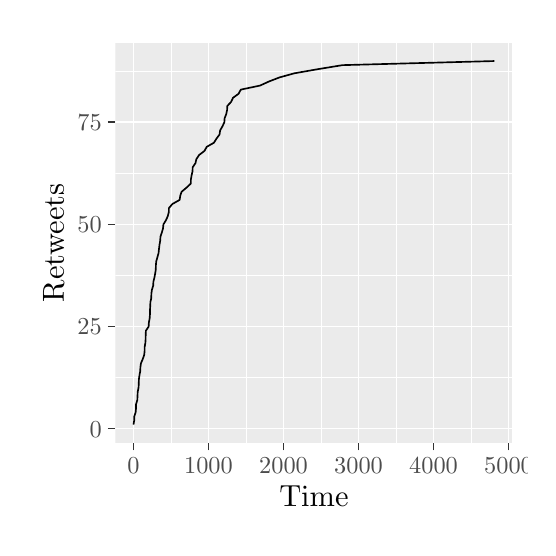
\begin{tikzpicture}[x=1pt,y=1pt]
\definecolor{fillColor}{RGB}{255,255,255}
\path[use as bounding box,fill=fillColor,fill opacity=0.00] (0,0) rectangle (180.67,180.67);
\begin{scope}
\path[clip] (  0.00,  0.00) rectangle (180.67,180.67);
\definecolor{drawColor}{RGB}{255,255,255}
\definecolor{fillColor}{RGB}{255,255,255}

\path[draw=drawColor,line width= 0.6pt,line join=round,line cap=round,fill=fillColor] (  0.00,  0.00) rectangle (180.68,180.68);
\end{scope}
\begin{scope}
\path[clip] ( 31.71, 30.69) rectangle (175.17,175.17);
\definecolor{fillColor}{gray}{0.92}

\path[fill=fillColor] ( 31.71, 30.69) rectangle (175.17,175.17);
\definecolor{drawColor}{RGB}{255,255,255}

\path[draw=drawColor,line width= 0.3pt,line join=round] ( 31.71, 54.23) --
	(175.17, 54.23);

\path[draw=drawColor,line width= 0.3pt,line join=round] ( 31.71, 91.12) --
	(175.17, 91.12);

\path[draw=drawColor,line width= 0.3pt,line join=round] ( 31.71,128.02) --
	(175.17,128.02);

\path[draw=drawColor,line width= 0.3pt,line join=round] ( 31.71,164.92) --
	(175.17,164.92);

\path[draw=drawColor,line width= 0.3pt,line join=round] ( 51.78, 30.69) --
	( 51.78,175.17);

\path[draw=drawColor,line width= 0.3pt,line join=round] ( 78.89, 30.69) --
	( 78.89,175.17);

\path[draw=drawColor,line width= 0.3pt,line join=round] (106.00, 30.69) --
	(106.00,175.17);

\path[draw=drawColor,line width= 0.3pt,line join=round] (133.11, 30.69) --
	(133.11,175.17);

\path[draw=drawColor,line width= 0.3pt,line join=round] (160.22, 30.69) --
	(160.22,175.17);

\path[draw=drawColor,line width= 0.6pt,line join=round] ( 31.71, 35.78) --
	(175.17, 35.78);

\path[draw=drawColor,line width= 0.6pt,line join=round] ( 31.71, 72.67) --
	(175.17, 72.67);

\path[draw=drawColor,line width= 0.6pt,line join=round] ( 31.71,109.57) --
	(175.17,109.57);

\path[draw=drawColor,line width= 0.6pt,line join=round] ( 31.71,146.47) --
	(175.17,146.47);

\path[draw=drawColor,line width= 0.6pt,line join=round] ( 38.23, 30.69) --
	( 38.23,175.17);

\path[draw=drawColor,line width= 0.6pt,line join=round] ( 65.34, 30.69) --
	( 65.34,175.17);

\path[draw=drawColor,line width= 0.6pt,line join=round] ( 92.45, 30.69) --
	( 92.45,175.17);

\path[draw=drawColor,line width= 0.6pt,line join=round] (119.55, 30.69) --
	(119.55,175.17);

\path[draw=drawColor,line width= 0.6pt,line join=round] (146.66, 30.69) --
	(146.66,175.17);

\path[draw=drawColor,line width= 0.6pt,line join=round] (173.77, 30.69) --
	(173.77,175.17);
\definecolor{drawColor}{RGB}{0,0,0}

\path[draw=drawColor,line width= 0.6pt,line join=round] ( 38.23, 37.25) --
	( 38.50, 38.73) --
	( 38.52, 40.21) --
	( 39.02, 41.68) --
	( 39.15, 43.16) --
	( 39.17, 44.63) --
	( 39.62, 46.11) --
	( 39.69, 47.58) --
	( 39.76, 49.06) --
	( 40.06, 50.54) --
	( 40.15, 52.01) --
	( 40.18, 53.49) --
	( 40.37, 54.96) --
	( 40.65, 56.44) --
	( 40.73, 57.92) --
	( 40.94, 59.39) --
	( 41.56, 60.87) --
	( 42.09, 62.34) --
	( 42.26, 63.82) --
	( 42.27, 65.30) --
	( 42.53, 66.77) --
	( 42.63, 68.25) --
	( 42.64, 69.72) --
	( 42.73, 71.20) --
	( 43.71, 72.67) --
	( 43.80, 74.15) --
	( 44.08, 75.63) --
	( 44.19, 77.10) --
	( 44.20, 78.58) --
	( 44.28, 80.05) --
	( 44.35, 81.53) --
	( 44.67, 83.01) --
	( 44.69, 84.48) --
	( 44.89, 85.96) --
	( 45.35, 87.43) --
	( 45.43, 88.91) --
	( 45.80, 90.39) --
	( 46.08, 91.86) --
	( 46.30, 93.34) --
	( 46.32, 94.81) --
	( 46.48, 96.29) --
	( 46.89, 97.76) --
	( 47.30, 99.24) --
	( 47.45,100.72) --
	( 47.63,102.19) --
	( 47.88,103.67) --
	( 47.98,105.14) --
	( 48.47,106.62) --
	( 48.90,108.10) --
	( 49.04,109.57) --
	( 49.95,111.05) --
	( 50.61,112.52) --
	( 51.00,114.00) --
	( 51.04,115.48) --
	( 52.29,116.95) --
	( 54.91,118.43) --
	( 55.13,119.90) --
	( 55.63,121.38) --
	( 57.38,122.85) --
	( 58.95,124.33) --
	( 58.98,125.81) --
	( 59.22,127.28) --
	( 59.57,128.76) --
	( 59.62,130.23) --
	( 60.63,131.71) --
	( 60.96,133.19) --
	( 61.95,134.66) --
	( 63.89,136.14) --
	( 64.70,137.61) --
	( 67.30,139.09) --
	( 68.22,140.57) --
	( 69.32,142.04) --
	( 69.53,143.52) --
	( 70.36,144.99) --
	( 71.07,146.47) --
	( 71.16,147.94) --
	( 71.75,149.42) --
	( 72.06,150.90) --
	( 72.13,152.37) --
	( 73.52,153.85) --
	( 74.19,155.32) --
	( 76.23,156.80) --
	( 77.00,158.28) --
	( 83.97,159.75) --
	( 87.21,161.23) --
	( 91.02,162.70) --
	( 96.37,164.18) --
	(104.79,165.66) --
	(113.76,167.13) --
	(168.65,168.61);
\end{scope}
\begin{scope}
\path[clip] (  0.00,  0.00) rectangle (180.67,180.67);
\definecolor{drawColor}{gray}{0.30}

\node[text=drawColor,anchor=base east,inner sep=0pt, outer sep=0pt, scale=  0.88] at ( 26.76, 32.75) {0};

\node[text=drawColor,anchor=base east,inner sep=0pt, outer sep=0pt, scale=  0.88] at ( 26.76, 69.64) {25};

\node[text=drawColor,anchor=base east,inner sep=0pt, outer sep=0pt, scale=  0.88] at ( 26.76,106.54) {50};

\node[text=drawColor,anchor=base east,inner sep=0pt, outer sep=0pt, scale=  0.88] at ( 26.76,143.44) {75};
\end{scope}
\begin{scope}
\path[clip] (  0.00,  0.00) rectangle (180.67,180.67);
\definecolor{drawColor}{gray}{0.20}

\path[draw=drawColor,line width= 0.6pt,line join=round] ( 28.96, 35.78) --
	( 31.71, 35.78);

\path[draw=drawColor,line width= 0.6pt,line join=round] ( 28.96, 72.67) --
	( 31.71, 72.67);

\path[draw=drawColor,line width= 0.6pt,line join=round] ( 28.96,109.57) --
	( 31.71,109.57);

\path[draw=drawColor,line width= 0.6pt,line join=round] ( 28.96,146.47) --
	( 31.71,146.47);
\end{scope}
\begin{scope}
\path[clip] (  0.00,  0.00) rectangle (180.67,180.67);
\definecolor{drawColor}{gray}{0.20}

\path[draw=drawColor,line width= 0.6pt,line join=round] ( 38.23, 27.94) --
	( 38.23, 30.69);

\path[draw=drawColor,line width= 0.6pt,line join=round] ( 65.34, 27.94) --
	( 65.34, 30.69);

\path[draw=drawColor,line width= 0.6pt,line join=round] ( 92.45, 27.94) --
	( 92.45, 30.69);

\path[draw=drawColor,line width= 0.6pt,line join=round] (119.55, 27.94) --
	(119.55, 30.69);

\path[draw=drawColor,line width= 0.6pt,line join=round] (146.66, 27.94) --
	(146.66, 30.69);

\path[draw=drawColor,line width= 0.6pt,line join=round] (173.77, 27.94) --
	(173.77, 30.69);
\end{scope}
\begin{scope}
\path[clip] (  0.00,  0.00) rectangle (180.67,180.67);
\definecolor{drawColor}{gray}{0.30}

\node[text=drawColor,anchor=base,inner sep=0pt, outer sep=0pt, scale=  0.88] at ( 38.23, 19.68) {0};

\node[text=drawColor,anchor=base,inner sep=0pt, outer sep=0pt, scale=  0.88] at ( 65.34, 19.68) {1000};

\node[text=drawColor,anchor=base,inner sep=0pt, outer sep=0pt, scale=  0.88] at ( 92.45, 19.68) {2000};

\node[text=drawColor,anchor=base,inner sep=0pt, outer sep=0pt, scale=  0.88] at (119.55, 19.68) {3000};

\node[text=drawColor,anchor=base,inner sep=0pt, outer sep=0pt, scale=  0.88] at (146.66, 19.68) {4000};

\node[text=drawColor,anchor=base,inner sep=0pt, outer sep=0pt, scale=  0.88] at (173.77, 19.68) {5000};
\end{scope}
\begin{scope}
\path[clip] (  0.00,  0.00) rectangle (180.67,180.67);
\definecolor{drawColor}{RGB}{0,0,0}

\node[text=drawColor,anchor=base,inner sep=0pt, outer sep=0pt, scale=  1.10] at (103.44,  7.64) {Time};
\end{scope}
\begin{scope}
\path[clip] (  0.00,  0.00) rectangle (180.67,180.67);
\definecolor{drawColor}{RGB}{0,0,0}

\node[text=drawColor,rotate= 90.00,anchor=base,inner sep=0pt, outer sep=0pt, scale=  1.10] at ( 13.08,102.93) {Retweets};
\end{scope}
\end{tikzpicture}

		\caption{First Simulation, $\overline\lambda=0.01$}
		\label{fig:sim1}
	\end{subfigure}%
	\begin{subfigure}{.5\textwidth}
		\centering
		% Created by tikzDevice version 0.12.3 on 2019-12-18 13:31:57
% !TEX encoding = UTF-8 Unicode
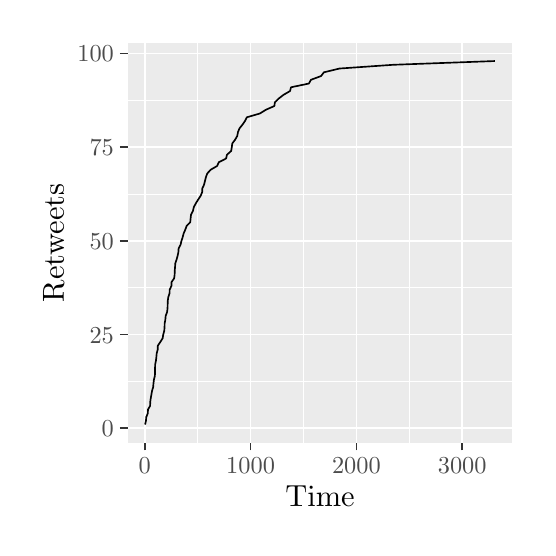
\begin{tikzpicture}[x=1pt,y=1pt]
\definecolor{fillColor}{RGB}{255,255,255}
\path[use as bounding box,fill=fillColor,fill opacity=0.00] (0,0) rectangle (180.67,180.67);
\begin{scope}
\path[clip] (  0.00,  0.00) rectangle (180.67,180.67);
\definecolor{drawColor}{RGB}{255,255,255}
\definecolor{fillColor}{RGB}{255,255,255}

\path[draw=drawColor,line width= 0.6pt,line join=round,line cap=round,fill=fillColor] (  0.00,  0.00) rectangle (180.68,180.68);
\end{scope}
\begin{scope}
\path[clip] ( 36.11, 30.69) rectangle (175.17,175.17);
\definecolor{fillColor}{gray}{0.92}

\path[fill=fillColor] ( 36.11, 30.69) rectangle (175.17,175.17);
\definecolor{drawColor}{RGB}{255,255,255}

\path[draw=drawColor,line width= 0.3pt,line join=round] ( 36.11, 52.83) --
	(175.17, 52.83);

\path[draw=drawColor,line width= 0.3pt,line join=round] ( 36.11, 86.68) --
	(175.17, 86.68);

\path[draw=drawColor,line width= 0.3pt,line join=round] ( 36.11,120.53) --
	(175.17,120.53);

\path[draw=drawColor,line width= 0.3pt,line join=round] ( 36.11,154.39) --
	(175.17,154.39);

\path[draw=drawColor,line width= 0.3pt,line join=round] ( 61.44, 30.69) --
	( 61.44,175.17);

\path[draw=drawColor,line width= 0.3pt,line join=round] ( 99.67, 30.69) --
	( 99.67,175.17);

\path[draw=drawColor,line width= 0.3pt,line join=round] (137.90, 30.69) --
	(137.90,175.17);

\path[draw=drawColor,line width= 0.6pt,line join=round] ( 36.11, 35.90) --
	(175.17, 35.90);

\path[draw=drawColor,line width= 0.6pt,line join=round] ( 36.11, 69.75) --
	(175.17, 69.75);

\path[draw=drawColor,line width= 0.6pt,line join=round] ( 36.11,103.61) --
	(175.17,103.61);

\path[draw=drawColor,line width= 0.6pt,line join=round] ( 36.11,137.46) --
	(175.17,137.46);

\path[draw=drawColor,line width= 0.6pt,line join=round] ( 36.11,171.32) --
	(175.17,171.32);

\path[draw=drawColor,line width= 0.6pt,line join=round] ( 42.32, 30.69) --
	( 42.32,175.17);

\path[draw=drawColor,line width= 0.6pt,line join=round] ( 80.55, 30.69) --
	( 80.55,175.17);

\path[draw=drawColor,line width= 0.6pt,line join=round] (118.78, 30.69) --
	(118.78,175.17);

\path[draw=drawColor,line width= 0.6pt,line join=round] (157.01, 30.69) --
	(157.01,175.17);
\definecolor{drawColor}{RGB}{0,0,0}

\path[draw=drawColor,line width= 0.6pt,line join=round] ( 42.43, 37.25) --
	( 42.75, 38.61) --
	( 42.85, 39.96) --
	( 43.42, 41.32) --
	( 43.47, 42.67) --
	( 44.25, 44.02) --
	( 44.28, 45.38) --
	( 44.47, 46.73) --
	( 44.71, 48.09) --
	( 44.94, 49.44) --
	( 45.35, 50.80) --
	( 45.45, 52.15) --
	( 45.63, 53.50) --
	( 45.97, 54.86) --
	( 46.01, 56.21) --
	( 46.03, 57.57) --
	( 46.05, 58.92) --
	( 46.34, 60.27) --
	( 46.50, 61.63) --
	( 46.62, 62.98) --
	( 46.99, 64.34) --
	( 47.00, 65.69) --
	( 47.89, 67.05) --
	( 48.77, 68.40) --
	( 48.98, 69.75) --
	( 49.35, 71.11) --
	( 49.46, 72.46) --
	( 49.50, 73.82) --
	( 49.75, 75.17) --
	( 49.86, 76.52) --
	( 50.37, 77.88) --
	( 50.54, 79.23) --
	( 50.58, 80.59) --
	( 50.62, 81.94) --
	( 50.82, 83.30) --
	( 51.27, 84.65) --
	( 51.31, 86.00) --
	( 51.95, 87.36) --
	( 51.97, 88.71) --
	( 52.92, 90.07) --
	( 53.11, 91.42) --
	( 53.13, 92.77) --
	( 53.25, 94.13) --
	( 53.34, 95.48) --
	( 53.80, 96.84) --
	( 54.17, 98.19) --
	( 54.46, 99.54) --
	( 54.54,100.90) --
	( 55.26,102.25) --
	( 55.55,103.61) --
	( 56.00,104.96) --
	( 56.36,106.32) --
	( 56.95,107.67) --
	( 57.44,109.02) --
	( 58.75,110.38) --
	( 58.87,111.73) --
	( 59.02,113.09) --
	( 59.73,114.44) --
	( 60.02,115.79) --
	( 60.74,117.15) --
	( 61.57,118.50) --
	( 62.47,119.86) --
	( 63.05,121.21) --
	( 63.11,122.57) --
	( 63.73,123.92) --
	( 64.07,125.27) --
	( 64.40,126.63) --
	( 64.89,127.98) --
	( 66.13,129.34) --
	( 68.46,130.69) --
	( 69.06,132.04) --
	( 71.71,133.40) --
	( 72.01,134.75) --
	( 73.53,136.11) --
	( 73.76,137.46) --
	( 73.93,138.82) --
	( 74.95,140.17) --
	( 75.72,141.52) --
	( 75.98,142.88) --
	( 76.51,144.23) --
	( 77.59,145.59) --
	( 78.54,146.94) --
	( 79.21,148.29) --
	( 83.89,149.65) --
	( 86.07,151.00) --
	( 89.15,152.36) --
	( 89.33,153.71) --
	( 90.72,155.07) --
	( 92.49,156.42) --
	( 94.81,157.77) --
	( 95.15,159.13) --
	(101.61,160.48) --
	(102.37,161.84) --
	(106.03,163.19) --
	(107.04,164.54) --
	(112.67,165.90) --
	(132.00,167.25) --
	(168.85,168.61);
\end{scope}
\begin{scope}
\path[clip] (  0.00,  0.00) rectangle (180.67,180.67);
\definecolor{drawColor}{gray}{0.30}

\node[text=drawColor,anchor=base east,inner sep=0pt, outer sep=0pt, scale=  0.88] at ( 31.16, 32.87) {0};

\node[text=drawColor,anchor=base east,inner sep=0pt, outer sep=0pt, scale=  0.88] at ( 31.16, 66.72) {25};

\node[text=drawColor,anchor=base east,inner sep=0pt, outer sep=0pt, scale=  0.88] at ( 31.16,100.58) {50};

\node[text=drawColor,anchor=base east,inner sep=0pt, outer sep=0pt, scale=  0.88] at ( 31.16,134.43) {75};

\node[text=drawColor,anchor=base east,inner sep=0pt, outer sep=0pt, scale=  0.88] at ( 31.16,168.29) {100};
\end{scope}
\begin{scope}
\path[clip] (  0.00,  0.00) rectangle (180.67,180.67);
\definecolor{drawColor}{gray}{0.20}

\path[draw=drawColor,line width= 0.6pt,line join=round] ( 33.36, 35.90) --
	( 36.11, 35.90);

\path[draw=drawColor,line width= 0.6pt,line join=round] ( 33.36, 69.75) --
	( 36.11, 69.75);

\path[draw=drawColor,line width= 0.6pt,line join=round] ( 33.36,103.61) --
	( 36.11,103.61);

\path[draw=drawColor,line width= 0.6pt,line join=round] ( 33.36,137.46) --
	( 36.11,137.46);

\path[draw=drawColor,line width= 0.6pt,line join=round] ( 33.36,171.32) --
	( 36.11,171.32);
\end{scope}
\begin{scope}
\path[clip] (  0.00,  0.00) rectangle (180.67,180.67);
\definecolor{drawColor}{gray}{0.20}

\path[draw=drawColor,line width= 0.6pt,line join=round] ( 42.32, 27.94) --
	( 42.32, 30.69);

\path[draw=drawColor,line width= 0.6pt,line join=round] ( 80.55, 27.94) --
	( 80.55, 30.69);

\path[draw=drawColor,line width= 0.6pt,line join=round] (118.78, 27.94) --
	(118.78, 30.69);

\path[draw=drawColor,line width= 0.6pt,line join=round] (157.01, 27.94) --
	(157.01, 30.69);
\end{scope}
\begin{scope}
\path[clip] (  0.00,  0.00) rectangle (180.67,180.67);
\definecolor{drawColor}{gray}{0.30}

\node[text=drawColor,anchor=base,inner sep=0pt, outer sep=0pt, scale=  0.88] at ( 42.32, 19.68) {0};

\node[text=drawColor,anchor=base,inner sep=0pt, outer sep=0pt, scale=  0.88] at ( 80.55, 19.68) {1000};

\node[text=drawColor,anchor=base,inner sep=0pt, outer sep=0pt, scale=  0.88] at (118.78, 19.68) {2000};

\node[text=drawColor,anchor=base,inner sep=0pt, outer sep=0pt, scale=  0.88] at (157.01, 19.68) {3000};
\end{scope}
\begin{scope}
\path[clip] (  0.00,  0.00) rectangle (180.67,180.67);
\definecolor{drawColor}{RGB}{0,0,0}

\node[text=drawColor,anchor=base,inner sep=0pt, outer sep=0pt, scale=  1.10] at (105.64,  7.64) {Time};
\end{scope}
\begin{scope}
\path[clip] (  0.00,  0.00) rectangle (180.67,180.67);
\definecolor{drawColor}{RGB}{0,0,0}

\node[text=drawColor,rotate= 90.00,anchor=base,inner sep=0pt, outer sep=0pt, scale=  1.10] at ( 13.08,102.93) {Retweets};
\end{scope}
\end{tikzpicture}

		\caption{Second Simulation, $\overline\lambda=0.01$}
		\label{fig:sim2}
	\end{subfigure}
\end{figure}

The simulated process behaves similarly to the account being studied. However, this does not represent the behaviour of all tweets, as the potential impact of the tweet and the interest it may generate influences the frequency of times.

\subsection{Using the intensity function of part b), compute the probability that a tweet from this user will get more than 10 retweets in the first hour, and the expected number of retweets of a tweet after 24 hours.}

The expected number of retweets are given by 
\[\mathbb{E}[N_t] = \int^t_0\lambda(x)dx \quad \Longrightarrow \quad \mathbb{E}[N_t] = \int^t_0 \theta e^{-\theta x} dx\]
where the intensity function is $ \lambda (t) = \theta e^{-\theta t},\ t>0$. 

However, when calculating the expected values for the previously defined $\theta = 0.001683839$ we get that $\mathbb{E}[N_t] \in (0,\ 1],\ \forall t>0$. Since the mean retweet process was previously scaled, in order to revert this behaviour, we will use the resulting probability to obtain the following adjusted expectation for $N_t$ while using the same $\overline\lambda = 0.01$ as in the simulation as the scaling factor of the expected retweets. 
\[\mathbb{E}'[N_t] = \frac{1}{\overline\lambda} \times \mathbb{E}[N_t] = \frac{1}{\overline\lambda}\int^t_0 \theta e^{-\theta x} dx\]

Therefore, the expected number of retweets after 24 hours (1440 minutes) would be
\[\mathbb{E}'[N_{1440}] = \frac{1}{\overline\lambda} \times \mathbb{E}[N_{1440}] = \frac{1}{0.01} \times 0.9114979 \sim 91\ retweets \] 

Similarly, the probability of $N_t$ being greater than $k$ is
\[P(N_{t} \geq k) = 1 - \sum_{t=0}^{k}\frac{\mathbb{E}'[N_{t}]^k e^{-\mathbb{E}'[N_{t}]}}{k!}\]
then
\[P(N_{60} \geq 10) = 1 - \sum_{t=0}^{10}\frac{\mathbb{E}'[N_{60}]^k e^{-\mathbb{E}'[N_{60}]}}{k!} = 0.3682237\]

\section{Exercise 2}
\subsection*{Question a}
The process $\bm{X} = \{X_t, \ t\geq 0\}$ is a continuous time Markov chain, as we are told that:
\begin{itemize}
	\item The customers arrive according ot a Poisson distribution with rate $\lambda$.
	\item Service times have an exponential distribution with rate $\mu$.
	\item There is no limit to the number of people in the system at any given time.
\end{itemize}

The \emph{state space} of our process is then $\{0\} \cup \mathbb{N}$. 
To obtain the infinitesimal generator, we observe that if $X_t = i$, then the only two possible transitions are into state $i+1$ if another customer joins the line and to state $i-1$ if a cashier finishes servicing its customer.

We know that the time until a new arrival takes place is just the interarrival time of a Poisson process, so it is exponentially distributed with rate $\lambda$.

The time until a customer is serviced is the minimum between the time it takes cashier $1$ to service its customer and the time it takes cashier $2$ to service theirs. 
This is the minimum of two exponentially distributed random variables, so it is also exponential with rate $\mu + \mu = 2\mu$.
\[
Q = \bordermatrix{% 
	 & 0 & 1 & 2 & 3 & \dots \cr
	0& -\lambda & \lambda  & 0        & 0        & \dots  \cr
	1 & \mu       & -(\lambda+\mu) & \lambda  & 0        & \dots  \cr
	2& 0        & 2\mu        & -(\lambda+2\mu) & \lambda  & \dots  \cr
	3 &0        & 0        & 2\mu        & (-\lambda + 2\mu) & \dots  \cr
	\vdots & \vdots   & \vdots   & \vdots   & \vdots   & \ddots
},
\]
The only rows that are different from the rest are the first and second ones.
In the case of the first one, this is because we can only go from state $X_t = 0$ to $X_{t+1} = 1$ if a customer arrives to the queue, and there is no customer to be serviced so that he can leave the queue.

In the case of the second row, now there is only one customer in the system and so he can only be serviced by a single cashier. This means that the chain will jump to state $0$ with rate $\mu$ if the cashier finishes servicing the customer or to state $2$ with rate $\lambda$ if another customer arrives.

From rows $3$ onwards, there is now at least two customers in the system, and as there are two cashiers the rate at which any one customer exits the system is the minimum between the time it takes the two cashiers to service their customer, which is exponentially distributed with rate $2\mu$ as we have explained previously.
Of course, customers can keep arriving at rate $\lambda$ as there is no limit to the amount of customers in the system.

\subsection*{Question b}
We know from the result in slide 21 of the continuous time Markov chain topic that the stationary distributions satisfies that $\bm{\pi}Q = 0$.
To find the stationary distribution we have to look for $\pi$ such that $\pi_i q_{ij} = \pi_j q_{ji}$.

A general expression for the elements $\pi_k, \ k\geq 1$ in terms of $\pi_0$ is the following:
\[
	\pi_k = \pi_0\left(\frac{\lambda}{\mu}\right)^k \frac{1}{2^{k-1}}
\]

We can obtain an expression for $\pi_0$ from Dobrow 7.6, as this is just a M/M/c queue where we have that
\[
	\pi_0^{-1} = \sum_{k=0}^{c-1} \left(\frac{\lambda}{\mu}\right)^k \frac{1}{k!} + \frac{\lambda / \mu}{c!} \left(\frac{1}{1 - \lambda/c\mu}\right)
\]
So four our case where $c=2$, the sum reduces to:
\[
	\pi_0 = \left(1 + \frac{\lambda}{\mu} + \frac{(\lambda/\mu)^2}{2}\left(\frac{1}{1 - \lambda/2\mu}\right)\right)^{-1}
\]

The long term expected number of people in the system can be obtained from Little's formula, which states that 
\[
	L = \lambda W
\]
Where $L$ is the long term average number of costumers in the system, $W$ is the long term average time of each customer in the system and $\lambda$ is the arrival rate (Dobrow 7.6).

Then, we can obtain the value for $L$ by calculating the expectation of the stationary distribution, as is stated in Dobrow 7.6
\[
	 L = \sum_{k \geq 0} k\pi_k
\]
\subsection*{Question c}
We can see that the only way an overtake can take place is if, once customer $j$ arrives to the queue, there is a customer $i$ being served and a free cashier. 
If there are two free cashiers, customer $j$ has nobody to overtake and if both cashiers are occupied he has to wait until one of them is free (and it does not matter which).

Then, in the case previously described we have that the service time for both customer $j$ and customer $i$ is exponentially distributed. As the exponential distribution is \emph{memoryless}, it does not matter how long customer $i$ has been waiting, as the probability of him being serviced before a given amount of time is the same.

Using the expression introduced in section 2 of \cite{baumann2018number}, we can find the expected number of overtakes as
\[
	\frac{\lambda}{\lambda + 2\mu},
\]
which is the particular expression for a M/M/2 queue like the one in our problem.

\subsection*{Question d}
The following code has been used to simulate the process for a given number of customers $k$.

\begin{listing}[H]
	\inputminted[firstline = 143, lastline = 166]{R}{../main.R}
	\caption{M/M/2 simulation}
	\label{lst:mm2sim}
\end{listing}
The generated exit times for a particular run of the simulation for 20 clients is:  1.4055, 16.1761, 35.5182, 16.8476, 24.2676, 19.0045, 21.4588, 25.0099, 23.4262, 25.6694, 35.5983, 38.0062, 42.7047,
39.5616, 48.4383, 40.1864, 41.2149, 48.9295, 41.5665, 46.4211 (in the relevant time unit).

\subsection*{Question e}
If two customers arrive every five minutes, this implies a rate $\lambda = \frac{2}{5}$ customers per minute. We also have that $\mathbf{E}\left[ \text{Cashier Serving Time}\right] = 4$. Since it is exponentially distributed, it rate has to be then $\mu = \frac{1}{4}$ customers per minute.


\textbf{Probability of overtaking:} We can get an estimate for this probability by calculating a trajectory of the chain, computing the number of overtakes and dividing by the total length of the chain. This has been done in \cref{lst:overtaking-sim}, where we have performed this procedure a large number of times then taken the average in order to obtain a better estimate.
\begin{listing}[H]
	\inputminted[firstline = 175, lastline = 187]{R}{../main.R}
	\caption{Overtaking Simulation}
	\label{lst:overtaking-sim}
\end{listing}
The resulting estimate for the probability of overtaking is $0.4717$.

The result when applying the equation introduced in the solution to question c is $\frac{\lambda}{\lambda + 2\mu} = 0.4444$. This is indeed quite close to our estimate, although not exactly the same due to the random nature of the process.

\textbf{Long Run Average of people in the system:}
In this case what we have done is calculate trajectories for the chain for an increasing number of customers. For each of this trajectories we have calculated the mean of the number of customers in the queue, and our final result is the average of the averages, to get a better estimate. The code can be seen in \cref{lst:longrun-sim}.
\begin{listing}[H]
	\inputminted[firstline = 198, lastline = 203]{R}{../main.R}
	\caption{Long Run Average Simulation}
	\label{lst:longrun-sim}
\end{listing}
The estimated average is then $2.2769$, and we can see a plot of the average number of customers in the system in \cref{fig:lravg}.
\begin{figure}[H]
	\centering
	% Created by tikzDevice version 0.12.3 on 2019-12-18 21:41:09
% !TEX encoding = UTF-8 Unicode
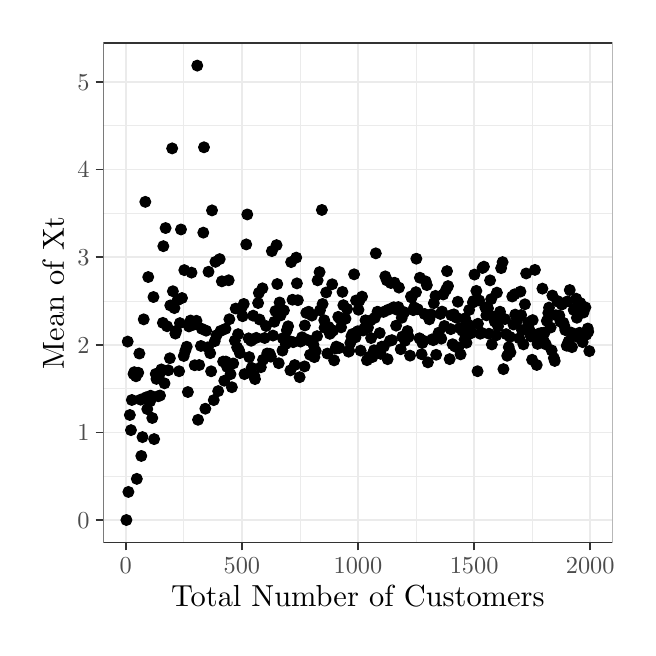
\begin{tikzpicture}[x=1pt,y=1pt]
\definecolor{fillColor}{RGB}{255,255,255}
\path[use as bounding box,fill=fillColor,fill opacity=0.00] (0,0) rectangle (216.81,216.81);
\begin{scope}
\path[clip] (  0.00,  0.00) rectangle (216.81,216.81);
\definecolor{drawColor}{RGB}{255,255,255}
\definecolor{fillColor}{RGB}{255,255,255}

\path[draw=drawColor,line width= 0.6pt,line join=round,line cap=round,fill=fillColor] (  0.00,  0.00) rectangle (216.81,216.81);
\end{scope}
\begin{scope}
\path[clip] ( 27.31, 30.69) rectangle (211.31,211.31);
\definecolor{fillColor}{RGB}{255,255,255}

\path[fill=fillColor] ( 27.31, 30.69) rectangle (211.31,211.31);
\definecolor{drawColor}{gray}{0.92}

\path[draw=drawColor,line width= 0.3pt,line join=round] ( 27.31, 54.72) --
	(211.31, 54.72);

\path[draw=drawColor,line width= 0.3pt,line join=round] ( 27.31, 86.38) --
	(211.31, 86.38);

\path[draw=drawColor,line width= 0.3pt,line join=round] ( 27.31,118.04) --
	(211.31,118.04);

\path[draw=drawColor,line width= 0.3pt,line join=round] ( 27.31,149.70) --
	(211.31,149.70);

\path[draw=drawColor,line width= 0.3pt,line join=round] ( 27.31,181.35) --
	(211.31,181.35);

\path[draw=drawColor,line width= 0.3pt,line join=round] ( 56.42, 30.69) --
	( 56.42,211.31);

\path[draw=drawColor,line width= 0.3pt,line join=round] ( 98.38, 30.69) --
	( 98.38,211.31);

\path[draw=drawColor,line width= 0.3pt,line join=round] (140.34, 30.69) --
	(140.34,211.31);

\path[draw=drawColor,line width= 0.3pt,line join=round] (182.29, 30.69) --
	(182.29,211.31);

\path[draw=drawColor,line width= 0.6pt,line join=round] ( 27.31, 38.90) --
	(211.31, 38.90);

\path[draw=drawColor,line width= 0.6pt,line join=round] ( 27.31, 70.55) --
	(211.31, 70.55);

\path[draw=drawColor,line width= 0.6pt,line join=round] ( 27.31,102.21) --
	(211.31,102.21);

\path[draw=drawColor,line width= 0.6pt,line join=round] ( 27.31,133.87) --
	(211.31,133.87);

\path[draw=drawColor,line width= 0.6pt,line join=round] ( 27.31,165.52) --
	(211.31,165.52);

\path[draw=drawColor,line width= 0.6pt,line join=round] ( 27.31,197.18) --
	(211.31,197.18);

\path[draw=drawColor,line width= 0.6pt,line join=round] ( 35.44, 30.69) --
	( 35.44,211.31);

\path[draw=drawColor,line width= 0.6pt,line join=round] ( 77.40, 30.69) --
	( 77.40,211.31);

\path[draw=drawColor,line width= 0.6pt,line join=round] (119.36, 30.69) --
	(119.36,211.31);

\path[draw=drawColor,line width= 0.6pt,line join=round] (161.32, 30.69) --
	(161.32,211.31);

\path[draw=drawColor,line width= 0.6pt,line join=round] (203.27, 30.69) --
	(203.27,211.31);
\definecolor{drawColor}{RGB}{0,0,0}
\definecolor{fillColor}{RGB}{0,0,0}

\path[draw=drawColor,line width= 0.4pt,line join=round,line cap=round,fill=fillColor] ( 35.68, 38.90) circle (  1.96);

\path[draw=drawColor,line width= 0.4pt,line join=round,line cap=round,fill=fillColor] ( 36.14,103.38) circle (  1.96);

\path[draw=drawColor,line width= 0.4pt,line join=round,line cap=round,fill=fillColor] ( 36.40, 49.05) circle (  1.96);

\path[draw=drawColor,line width= 0.4pt,line join=round,line cap=round,fill=fillColor] ( 36.92, 76.85) circle (  1.96);

\path[draw=drawColor,line width= 0.4pt,line join=round,line cap=round,fill=fillColor] ( 37.32, 71.38) circle (  1.96);

\path[draw=drawColor,line width= 0.4pt,line join=round,line cap=round,fill=fillColor] ( 37.64, 82.27) circle (  1.96);

\path[draw=drawColor,line width= 0.4pt,line join=round,line cap=round,fill=fillColor] ( 38.25, 91.69) circle (  1.96);

\path[draw=drawColor,line width= 0.4pt,line join=round,line cap=round,fill=fillColor] ( 38.51, 92.32) circle (  1.96);

\path[draw=drawColor,line width= 0.4pt,line join=round,line cap=round,fill=fillColor] ( 39.15, 90.83) circle (  1.96);

\path[draw=drawColor,line width= 0.4pt,line join=round,line cap=round,fill=fillColor] ( 39.44, 53.77) circle (  1.96);

\path[draw=drawColor,line width= 0.4pt,line join=round,line cap=round,fill=fillColor] ( 39.96, 92.13) circle (  1.96);

\path[draw=drawColor,line width= 0.4pt,line join=round,line cap=round,fill=fillColor] ( 40.36, 99.05) circle (  1.96);

\path[draw=drawColor,line width= 0.4pt,line join=round,line cap=round,fill=fillColor] ( 40.79, 82.39) circle (  1.96);

\path[draw=drawColor,line width= 0.4pt,line join=round,line cap=round,fill=fillColor] ( 41.06, 62.05) circle (  1.96);

\path[draw=drawColor,line width= 0.4pt,line join=round,line cap=round,fill=fillColor] ( 41.49, 68.86) circle (  1.96);

\path[draw=drawColor,line width= 0.4pt,line join=round,line cap=round,fill=fillColor] ( 41.93,111.41) circle (  1.96);

\path[draw=drawColor,line width= 0.4pt,line join=round,line cap=round,fill=fillColor] ( 42.51,153.87) circle (  1.96);

\path[draw=drawColor,line width= 0.4pt,line join=round,line cap=round,fill=fillColor] ( 42.71, 83.20) circle (  1.96);

\path[draw=drawColor,line width= 0.4pt,line join=round,line cap=round,fill=fillColor] ( 43.22, 78.99) circle (  1.96);

\path[draw=drawColor,line width= 0.4pt,line join=round,line cap=round,fill=fillColor] ( 43.56,126.70) circle (  1.96);

\path[draw=drawColor,line width= 0.4pt,line join=round,line cap=round,fill=fillColor] ( 44.24, 81.79) circle (  1.96);

\path[draw=drawColor,line width= 0.4pt,line join=round,line cap=round,fill=fillColor] ( 44.42, 83.82) circle (  1.96);

\path[draw=drawColor,line width= 0.4pt,line join=round,line cap=round,fill=fillColor] ( 45.03, 75.76) circle (  1.96);

\path[draw=drawColor,line width= 0.4pt,line join=round,line cap=round,fill=fillColor] ( 45.45,119.47) circle (  1.96);

\path[draw=drawColor,line width= 0.4pt,line join=round,line cap=round,fill=fillColor] ( 45.70, 68.14) circle (  1.96);

\path[draw=drawColor,line width= 0.4pt,line join=round,line cap=round,fill=fillColor] ( 46.27, 91.68) circle (  1.96);

\path[draw=drawColor,line width= 0.4pt,line join=round,line cap=round,fill=fillColor] ( 46.53, 89.89) circle (  1.96);

\path[draw=drawColor,line width= 0.4pt,line join=round,line cap=round,fill=fillColor] ( 47.16, 83.62) circle (  1.96);

\path[draw=drawColor,line width= 0.4pt,line join=round,line cap=round,fill=fillColor] ( 47.56, 91.39) circle (  1.96);

\path[draw=drawColor,line width= 0.4pt,line join=round,line cap=round,fill=fillColor] ( 47.83, 83.89) circle (  1.96);

\path[draw=drawColor,line width= 0.4pt,line join=round,line cap=round,fill=fillColor] ( 48.31, 93.32) circle (  1.96);

\path[draw=drawColor,line width= 0.4pt,line join=round,line cap=round,fill=fillColor] ( 48.86,110.14) circle (  1.96);

\path[draw=drawColor,line width= 0.4pt,line join=round,line cap=round,fill=fillColor] ( 49.02,137.85) circle (  1.96);

\path[draw=drawColor,line width= 0.4pt,line join=round,line cap=round,fill=fillColor] ( 49.45, 88.29) circle (  1.96);

\path[draw=drawColor,line width= 0.4pt,line join=round,line cap=round,fill=fillColor] ( 49.83,144.40) circle (  1.96);

\path[draw=drawColor,line width= 0.4pt,line join=round,line cap=round,fill=fillColor] ( 50.37,108.91) circle (  1.96);

\path[draw=drawColor,line width= 0.4pt,line join=round,line cap=round,fill=fillColor] ( 50.81, 93.01) circle (  1.96);

\path[draw=drawColor,line width= 0.4pt,line join=round,line cap=round,fill=fillColor] ( 51.38, 97.36) circle (  1.96);

\path[draw=drawColor,line width= 0.4pt,line join=round,line cap=round,fill=fillColor] ( 51.52,116.44) circle (  1.96);

\path[draw=drawColor,line width= 0.4pt,line join=round,line cap=round,fill=fillColor] ( 52.21,173.19) circle (  1.96);

\path[draw=drawColor,line width= 0.4pt,line join=round,line cap=round,fill=fillColor] ( 52.47,121.57) circle (  1.96);

\path[draw=drawColor,line width= 0.4pt,line join=round,line cap=round,fill=fillColor] ( 53.02,115.48) circle (  1.96);

\path[draw=drawColor,line width= 0.4pt,line join=round,line cap=round,fill=fillColor] ( 53.37,106.27) circle (  1.96);

\path[draw=drawColor,line width= 0.4pt,line join=round,line cap=round,fill=fillColor] ( 53.67,107.28) circle (  1.96);

\path[draw=drawColor,line width= 0.4pt,line join=round,line cap=round,fill=fillColor] ( 54.18,118.37) circle (  1.96);

\path[draw=drawColor,line width= 0.4pt,line join=round,line cap=round,fill=fillColor] ( 54.72, 92.66) circle (  1.96);

\path[draw=drawColor,line width= 0.4pt,line join=round,line cap=round,fill=fillColor] ( 55.01,110.05) circle (  1.96);

\path[draw=drawColor,line width= 0.4pt,line join=round,line cap=round,fill=fillColor] ( 55.40,143.89) circle (  1.96);

\path[draw=drawColor,line width= 0.4pt,line join=round,line cap=round,fill=fillColor] ( 55.76,119.11) circle (  1.96);

\path[draw=drawColor,line width= 0.4pt,line join=round,line cap=round,fill=fillColor] ( 56.40, 98.17) circle (  1.96);

\path[draw=drawColor,line width= 0.4pt,line join=round,line cap=round,fill=fillColor] ( 56.60,129.20) circle (  1.96);

\path[draw=drawColor,line width= 0.4pt,line join=round,line cap=round,fill=fillColor] ( 56.95,100.03) circle (  1.96);

\path[draw=drawColor,line width= 0.4pt,line join=round,line cap=round,fill=fillColor] ( 57.47,101.52) circle (  1.96);

\path[draw=drawColor,line width= 0.4pt,line join=round,line cap=round,fill=fillColor] ( 57.89, 85.15) circle (  1.96);

\path[draw=drawColor,line width= 0.4pt,line join=round,line cap=round,fill=fillColor] ( 58.28,108.85) circle (  1.96);

\path[draw=drawColor,line width= 0.4pt,line join=round,line cap=round,fill=fillColor] ( 58.86,110.99) circle (  1.96);

\path[draw=drawColor,line width= 0.4pt,line join=round,line cap=round,fill=fillColor] ( 59.20,128.30) circle (  1.96);

\path[draw=drawColor,line width= 0.4pt,line join=round,line cap=round,fill=fillColor] ( 59.62,109.64) circle (  1.96);

\path[draw=drawColor,line width= 0.4pt,line join=round,line cap=round,fill=fillColor] ( 59.96,109.49) circle (  1.96);

\path[draw=drawColor,line width= 0.4pt,line join=round,line cap=round,fill=fillColor] ( 60.35, 94.82) circle (  1.96);

\path[draw=drawColor,line width= 0.4pt,line join=round,line cap=round,fill=fillColor] ( 61.01,110.89) circle (  1.96);

\path[draw=drawColor,line width= 0.4pt,line join=round,line cap=round,fill=fillColor] ( 61.28,203.10) circle (  1.96);

\path[draw=drawColor,line width= 0.4pt,line join=round,line cap=round,fill=fillColor] ( 61.56, 75.11) circle (  1.96);

\path[draw=drawColor,line width= 0.4pt,line join=round,line cap=round,fill=fillColor] ( 61.98, 94.90) circle (  1.96);

\path[draw=drawColor,line width= 0.4pt,line join=round,line cap=round,fill=fillColor] ( 62.60,101.80) circle (  1.96);

\path[draw=drawColor,line width= 0.4pt,line join=round,line cap=round,fill=fillColor] ( 62.94,107.99) circle (  1.96);

\path[draw=drawColor,line width= 0.4pt,line join=round,line cap=round,fill=fillColor] ( 63.46,142.74) circle (  1.96);

\path[draw=drawColor,line width= 0.4pt,line join=round,line cap=round,fill=fillColor] ( 63.71,173.58) circle (  1.96);

\path[draw=drawColor,line width= 0.4pt,line join=round,line cap=round,fill=fillColor] ( 64.20, 79.12) circle (  1.96);

\path[draw=drawColor,line width= 0.4pt,line join=round,line cap=round,fill=fillColor] ( 64.50,107.31) circle (  1.96);

\path[draw=drawColor,line width= 0.4pt,line join=round,line cap=round,fill=fillColor] ( 65.11,101.31) circle (  1.96);

\path[draw=drawColor,line width= 0.4pt,line join=round,line cap=round,fill=fillColor] ( 65.35,128.61) circle (  1.96);

\path[draw=drawColor,line width= 0.4pt,line join=round,line cap=round,fill=fillColor] ( 65.95, 99.18) circle (  1.96);

\path[draw=drawColor,line width= 0.4pt,line join=round,line cap=round,fill=fillColor] ( 66.29, 92.64) circle (  1.96);

\path[draw=drawColor,line width= 0.4pt,line join=round,line cap=round,fill=fillColor] ( 66.61,150.78) circle (  1.96);

\path[draw=drawColor,line width= 0.4pt,line join=round,line cap=round,fill=fillColor] ( 67.24, 82.23) circle (  1.96);

\path[draw=drawColor,line width= 0.4pt,line join=round,line cap=round,fill=fillColor] ( 67.61,103.53) circle (  1.96);

\path[draw=drawColor,line width= 0.4pt,line join=round,line cap=round,fill=fillColor] ( 67.84,132.19) circle (  1.96);

\path[draw=drawColor,line width= 0.4pt,line join=round,line cap=round,fill=fillColor] ( 68.25,105.66) circle (  1.96);

\path[draw=drawColor,line width= 0.4pt,line join=round,line cap=round,fill=fillColor] ( 68.84, 85.48) circle (  1.96);

\path[draw=drawColor,line width= 0.4pt,line join=round,line cap=round,fill=fillColor] ( 69.39,133.18) circle (  1.96);

\path[draw=drawColor,line width= 0.4pt,line join=round,line cap=round,fill=fillColor] ( 69.72,107.23) circle (  1.96);

\path[draw=drawColor,line width= 0.4pt,line join=round,line cap=round,fill=fillColor] ( 70.17,125.15) circle (  1.96);

\path[draw=drawColor,line width= 0.4pt,line join=round,line cap=round,fill=fillColor] ( 70.63, 96.15) circle (  1.96);

\path[draw=drawColor,line width= 0.4pt,line join=round,line cap=round,fill=fillColor] ( 71.05, 89.22) circle (  1.96);

\path[draw=drawColor,line width= 0.4pt,line join=round,line cap=round,fill=fillColor] ( 71.47,107.99) circle (  1.96);

\path[draw=drawColor,line width= 0.4pt,line join=round,line cap=round,fill=fillColor] ( 71.62, 96.15) circle (  1.96);

\path[draw=drawColor,line width= 0.4pt,line join=round,line cap=round,fill=fillColor] ( 72.08, 94.23) circle (  1.96);

\path[draw=drawColor,line width= 0.4pt,line join=round,line cap=round,fill=fillColor] ( 72.63,125.53) circle (  1.96);

\path[draw=drawColor,line width= 0.4pt,line join=round,line cap=round,fill=fillColor] ( 72.88,111.45) circle (  1.96);

\path[draw=drawColor,line width= 0.4pt,line join=round,line cap=round,fill=fillColor] ( 73.31, 91.61) circle (  1.96);

\path[draw=drawColor,line width= 0.4pt,line join=round,line cap=round,fill=fillColor] ( 73.79, 86.88) circle (  1.96);

\path[draw=drawColor,line width= 0.4pt,line join=round,line cap=round,fill=fillColor] ( 74.29, 95.48) circle (  1.96);

\path[draw=drawColor,line width= 0.4pt,line join=round,line cap=round,fill=fillColor] ( 74.87,103.75) circle (  1.96);

\path[draw=drawColor,line width= 0.4pt,line join=round,line cap=round,fill=fillColor] ( 75.16,115.31) circle (  1.96);

\path[draw=drawColor,line width= 0.4pt,line join=round,line cap=round,fill=fillColor] ( 75.69,101.28) circle (  1.96);

\path[draw=drawColor,line width= 0.4pt,line join=round,line cap=round,fill=fillColor] ( 76.04,106.06) circle (  1.96);

\path[draw=drawColor,line width= 0.4pt,line join=round,line cap=round,fill=fillColor] ( 76.32,100.31) circle (  1.96);

\path[draw=drawColor,line width= 0.4pt,line join=round,line cap=round,fill=fillColor] ( 76.68, 99.21) circle (  1.96);

\path[draw=drawColor,line width= 0.4pt,line join=round,line cap=round,fill=fillColor] ( 77.12,115.12) circle (  1.96);

\path[draw=drawColor,line width= 0.4pt,line join=round,line cap=round,fill=fillColor] ( 77.67,112.54) circle (  1.96);

\path[draw=drawColor,line width= 0.4pt,line join=round,line cap=round,fill=fillColor] ( 78.10,116.98) circle (  1.96);

\path[draw=drawColor,line width= 0.4pt,line join=round,line cap=round,fill=fillColor] ( 78.34, 91.63) circle (  1.96);

\path[draw=drawColor,line width= 0.4pt,line join=round,line cap=round,fill=fillColor] ( 78.98,138.49) circle (  1.96);

\path[draw=drawColor,line width= 0.4pt,line join=round,line cap=round,fill=fillColor] ( 79.36,149.32) circle (  1.96);

\path[draw=drawColor,line width= 0.4pt,line join=round,line cap=round,fill=fillColor] ( 79.84,104.54) circle (  1.96);

\path[draw=drawColor,line width= 0.4pt,line join=round,line cap=round,fill=fillColor] ( 80.06, 97.77) circle (  1.96);

\path[draw=drawColor,line width= 0.4pt,line join=round,line cap=round,fill=fillColor] ( 80.74,103.66) circle (  1.96);

\path[draw=drawColor,line width= 0.4pt,line join=round,line cap=round,fill=fillColor] ( 80.92, 93.89) circle (  1.96);

\path[draw=drawColor,line width= 0.4pt,line join=round,line cap=round,fill=fillColor] ( 81.48,112.74) circle (  1.96);

\path[draw=drawColor,line width= 0.4pt,line join=round,line cap=round,fill=fillColor] ( 81.90, 90.97) circle (  1.96);

\path[draw=drawColor,line width= 0.4pt,line join=round,line cap=round,fill=fillColor] ( 82.15, 89.83) circle (  1.96);

\path[draw=drawColor,line width= 0.4pt,line join=round,line cap=round,fill=fillColor] ( 82.61,104.72) circle (  1.96);

\path[draw=drawColor,line width= 0.4pt,line join=round,line cap=round,fill=fillColor] ( 83.27,117.31) circle (  1.96);

\path[draw=drawColor,line width= 0.4pt,line join=round,line cap=round,fill=fillColor] ( 83.53,120.95) circle (  1.96);

\path[draw=drawColor,line width= 0.4pt,line join=round,line cap=round,fill=fillColor] ( 83.80,111.34) circle (  1.96);

\path[draw=drawColor,line width= 0.4pt,line join=round,line cap=round,fill=fillColor] ( 84.25, 94.10) circle (  1.96);

\path[draw=drawColor,line width= 0.4pt,line join=round,line cap=round,fill=fillColor] ( 84.84,122.62) circle (  1.96);

\path[draw=drawColor,line width= 0.4pt,line join=round,line cap=round,fill=fillColor] ( 85.04, 96.80) circle (  1.96);

\path[draw=drawColor,line width= 0.4pt,line join=round,line cap=round,fill=fillColor] ( 85.64,104.67) circle (  1.96);

\path[draw=drawColor,line width= 0.4pt,line join=round,line cap=round,fill=fillColor] ( 86.13,109.00) circle (  1.96);

\path[draw=drawColor,line width= 0.4pt,line join=round,line cap=round,fill=fillColor] ( 86.55, 99.09) circle (  1.96);

\path[draw=drawColor,line width= 0.4pt,line join=round,line cap=round,fill=fillColor] ( 87.02, 98.78) circle (  1.96);

\path[draw=drawColor,line width= 0.4pt,line join=round,line cap=round,fill=fillColor] ( 87.44, 99.00) circle (  1.96);

\path[draw=drawColor,line width= 0.4pt,line join=round,line cap=round,fill=fillColor] ( 87.88, 97.91) circle (  1.96);

\path[draw=drawColor,line width= 0.4pt,line join=round,line cap=round,fill=fillColor] ( 88.24,136.07) circle (  1.96);

\path[draw=drawColor,line width= 0.4pt,line join=round,line cap=round,fill=fillColor] ( 88.64,105.55) circle (  1.96);

\path[draw=drawColor,line width= 0.4pt,line join=round,line cap=round,fill=fillColor] ( 89.12,110.53) circle (  1.96);

\path[draw=drawColor,line width= 0.4pt,line join=round,line cap=round,fill=fillColor] ( 89.52,114.42) circle (  1.96);

\path[draw=drawColor,line width= 0.4pt,line join=round,line cap=round,fill=fillColor] ( 89.94,138.23) circle (  1.96);

\path[draw=drawColor,line width= 0.4pt,line join=round,line cap=round,fill=fillColor] ( 90.19,124.17) circle (  1.96);

\path[draw=drawColor,line width= 0.4pt,line join=round,line cap=round,fill=fillColor] ( 90.73, 95.56) circle (  1.96);

\path[draw=drawColor,line width= 0.4pt,line join=round,line cap=round,fill=fillColor] ( 91.04,117.52) circle (  1.96);

\path[draw=drawColor,line width= 0.4pt,line join=round,line cap=round,fill=fillColor] ( 91.36,112.81) circle (  1.96);

\path[draw=drawColor,line width= 0.4pt,line join=round,line cap=round,fill=fillColor] ( 92.06,100.12) circle (  1.96);

\path[draw=drawColor,line width= 0.4pt,line join=round,line cap=round,fill=fillColor] ( 92.19,104.59) circle (  1.96);

\path[draw=drawColor,line width= 0.4pt,line join=round,line cap=round,fill=fillColor] ( 92.60,114.64) circle (  1.96);

\path[draw=drawColor,line width= 0.4pt,line join=round,line cap=round,fill=fillColor] ( 93.27,102.51) circle (  1.96);

\path[draw=drawColor,line width= 0.4pt,line join=round,line cap=round,fill=fillColor] ( 93.65,107.47) circle (  1.96);

\path[draw=drawColor,line width= 0.4pt,line join=round,line cap=round,fill=fillColor] ( 94.12,108.91) circle (  1.96);

\path[draw=drawColor,line width= 0.4pt,line join=round,line cap=round,fill=fillColor] ( 94.32,103.68) circle (  1.96);

\path[draw=drawColor,line width= 0.4pt,line join=round,line cap=round,fill=fillColor] ( 94.94, 92.98) circle (  1.96);

\path[draw=drawColor,line width= 0.4pt,line join=round,line cap=round,fill=fillColor] ( 95.20,132.10) circle (  1.96);

\path[draw=drawColor,line width= 0.4pt,line join=round,line cap=round,fill=fillColor] ( 95.69,118.50) circle (  1.96);

\path[draw=drawColor,line width= 0.4pt,line join=round,line cap=round,fill=fillColor] ( 95.95,103.16) circle (  1.96);

\path[draw=drawColor,line width= 0.4pt,line join=round,line cap=round,fill=fillColor] ( 96.49, 94.89) circle (  1.96);

\path[draw=drawColor,line width= 0.4pt,line join=round,line cap=round,fill=fillColor] ( 97.05,133.72) circle (  1.96);

\path[draw=drawColor,line width= 0.4pt,line join=round,line cap=round,fill=fillColor] ( 97.29,124.41) circle (  1.96);

\path[draw=drawColor,line width= 0.4pt,line join=round,line cap=round,fill=fillColor] ( 97.63,118.33) circle (  1.96);

\path[draw=drawColor,line width= 0.4pt,line join=round,line cap=round,fill=fillColor] ( 98.27, 90.52) circle (  1.96);

\path[draw=drawColor,line width= 0.4pt,line join=round,line cap=round,fill=fillColor] ( 98.57,103.38) circle (  1.96);

\path[draw=drawColor,line width= 0.4pt,line join=round,line cap=round,fill=fillColor] ( 99.15,104.94) circle (  1.96);

\path[draw=drawColor,line width= 0.4pt,line join=round,line cap=round,fill=fillColor] ( 99.52,104.14) circle (  1.96);

\path[draw=drawColor,line width= 0.4pt,line join=round,line cap=round,fill=fillColor] (100.05, 94.41) circle (  1.96);

\path[draw=drawColor,line width= 0.4pt,line join=round,line cap=round,fill=fillColor] (100.16,109.20) circle (  1.96);

\path[draw=drawColor,line width= 0.4pt,line join=round,line cap=round,fill=fillColor] (100.67,113.74) circle (  1.96);

\path[draw=drawColor,line width= 0.4pt,line join=round,line cap=round,fill=fillColor] (101.06,103.98) circle (  1.96);

\path[draw=drawColor,line width= 0.4pt,line join=round,line cap=round,fill=fillColor] (101.53,114.17) circle (  1.96);

\path[draw=drawColor,line width= 0.4pt,line join=round,line cap=round,fill=fillColor] (102.03, 98.61) circle (  1.96);

\path[draw=drawColor,line width= 0.4pt,line join=round,line cap=round,fill=fillColor] (102.50, 98.66) circle (  1.96);

\path[draw=drawColor,line width= 0.4pt,line join=round,line cap=round,fill=fillColor] (102.71,112.77) circle (  1.96);

\path[draw=drawColor,line width= 0.4pt,line join=round,line cap=round,fill=fillColor] (103.26,102.26) circle (  1.96);

\path[draw=drawColor,line width= 0.4pt,line join=round,line cap=round,fill=fillColor] (103.60, 97.76) circle (  1.96);

\path[draw=drawColor,line width= 0.4pt,line join=round,line cap=round,fill=fillColor] (104.08, 99.96) circle (  1.96);

\path[draw=drawColor,line width= 0.4pt,line join=round,line cap=round,fill=fillColor] (104.58,105.34) circle (  1.96);

\path[draw=drawColor,line width= 0.4pt,line join=round,line cap=round,fill=fillColor] (104.77,125.51) circle (  1.96);

\path[draw=drawColor,line width= 0.4pt,line join=round,line cap=round,fill=fillColor] (105.48,128.48) circle (  1.96);

\path[draw=drawColor,line width= 0.4pt,line join=round,line cap=round,fill=fillColor] (105.63,114.69) circle (  1.96);

\path[draw=drawColor,line width= 0.4pt,line join=round,line cap=round,fill=fillColor] (106.31,150.94) circle (  1.96);

\path[draw=drawColor,line width= 0.4pt,line join=round,line cap=round,fill=fillColor] (106.56,116.97) circle (  1.96);

\path[draw=drawColor,line width= 0.4pt,line join=round,line cap=round,fill=fillColor] (107.16,111.10) circle (  1.96);

\path[draw=drawColor,line width= 0.4pt,line join=round,line cap=round,fill=fillColor] (107.28,108.40) circle (  1.96);

\path[draw=drawColor,line width= 0.4pt,line join=round,line cap=round,fill=fillColor] (107.86,121.12) circle (  1.96);

\path[draw=drawColor,line width= 0.4pt,line join=round,line cap=round,fill=fillColor] (108.31, 99.05) circle (  1.96);

\path[draw=drawColor,line width= 0.4pt,line join=round,line cap=round,fill=fillColor] (108.75,108.67) circle (  1.96);

\path[draw=drawColor,line width= 0.4pt,line join=round,line cap=round,fill=fillColor] (109.19,106.18) circle (  1.96);

\path[draw=drawColor,line width= 0.4pt,line join=round,line cap=round,fill=fillColor] (109.69,106.85) circle (  1.96);

\path[draw=drawColor,line width= 0.4pt,line join=round,line cap=round,fill=fillColor] (110.03,124.09) circle (  1.96);

\path[draw=drawColor,line width= 0.4pt,line join=round,line cap=round,fill=fillColor] (110.38,107.37) circle (  1.96);

\path[draw=drawColor,line width= 0.4pt,line join=round,line cap=round,fill=fillColor] (110.74, 96.59) circle (  1.96);

\path[draw=drawColor,line width= 0.4pt,line join=round,line cap=round,fill=fillColor] (111.29,100.86) circle (  1.96);

\path[draw=drawColor,line width= 0.4pt,line join=round,line cap=round,fill=fillColor] (111.54,101.58) circle (  1.96);

\path[draw=drawColor,line width= 0.4pt,line join=round,line cap=round,fill=fillColor] (112.22,112.32) circle (  1.96);

\path[draw=drawColor,line width= 0.4pt,line join=round,line cap=round,fill=fillColor] (112.61,101.06) circle (  1.96);

\path[draw=drawColor,line width= 0.4pt,line join=round,line cap=round,fill=fillColor] (112.89,111.56) circle (  1.96);

\path[draw=drawColor,line width= 0.4pt,line join=round,line cap=round,fill=fillColor] (113.25,108.52) circle (  1.96);

\path[draw=drawColor,line width= 0.4pt,line join=round,line cap=round,fill=fillColor] (113.74,121.33) circle (  1.96);

\path[draw=drawColor,line width= 0.4pt,line join=round,line cap=round,fill=fillColor] (114.07,116.53) circle (  1.96);

\path[draw=drawColor,line width= 0.4pt,line join=round,line cap=round,fill=fillColor] (114.59,111.64) circle (  1.96);

\path[draw=drawColor,line width= 0.4pt,line join=round,line cap=round,fill=fillColor] (114.85,111.65) circle (  1.96);

\path[draw=drawColor,line width= 0.4pt,line join=round,line cap=round,fill=fillColor] (115.42,115.17) circle (  1.96);

\path[draw=drawColor,line width= 0.4pt,line join=round,line cap=round,fill=fillColor] (115.97, 99.73) circle (  1.96);

\path[draw=drawColor,line width= 0.4pt,line join=round,line cap=round,fill=fillColor] (116.19,100.08) circle (  1.96);

\path[draw=drawColor,line width= 0.4pt,line join=round,line cap=round,fill=fillColor] (116.59,102.91) circle (  1.96);

\path[draw=drawColor,line width= 0.4pt,line join=round,line cap=round,fill=fillColor] (116.97,105.30) circle (  1.96);

\path[draw=drawColor,line width= 0.4pt,line join=round,line cap=round,fill=fillColor] (117.36,106.10) circle (  1.96);

\path[draw=drawColor,line width= 0.4pt,line join=round,line cap=round,fill=fillColor] (117.96,127.68) circle (  1.96);

\path[draw=drawColor,line width= 0.4pt,line join=round,line cap=round,fill=fillColor] (118.48,104.92) circle (  1.96);

\path[draw=drawColor,line width= 0.4pt,line join=round,line cap=round,fill=fillColor] (118.65,118.24) circle (  1.96);

\path[draw=drawColor,line width= 0.4pt,line join=round,line cap=round,fill=fillColor] (119.28,107.13) circle (  1.96);

\path[draw=drawColor,line width= 0.4pt,line join=round,line cap=round,fill=fillColor] (119.54,114.87) circle (  1.96);

\path[draw=drawColor,line width= 0.4pt,line join=round,line cap=round,fill=fillColor] (119.87,118.17) circle (  1.96);

\path[draw=drawColor,line width= 0.4pt,line join=round,line cap=round,fill=fillColor] (120.31,100.12) circle (  1.96);

\path[draw=drawColor,line width= 0.4pt,line join=round,line cap=round,fill=fillColor] (120.83,119.62) circle (  1.96);

\path[draw=drawColor,line width= 0.4pt,line join=round,line cap=round,fill=fillColor] (121.22,107.37) circle (  1.96);

\path[draw=drawColor,line width= 0.4pt,line join=round,line cap=round,fill=fillColor] (121.56,108.01) circle (  1.96);

\path[draw=drawColor,line width= 0.4pt,line join=round,line cap=round,fill=fillColor] (122.07,111.06) circle (  1.96);

\path[draw=drawColor,line width= 0.4pt,line join=round,line cap=round,fill=fillColor] (122.59, 96.66) circle (  1.96);

\path[draw=drawColor,line width= 0.4pt,line join=round,line cap=round,fill=fillColor] (122.97,108.45) circle (  1.96);

\path[draw=drawColor,line width= 0.4pt,line join=round,line cap=round,fill=fillColor] (123.44, 97.90) circle (  1.96);

\path[draw=drawColor,line width= 0.4pt,line join=round,line cap=round,fill=fillColor] (123.83,110.99) circle (  1.96);

\path[draw=drawColor,line width= 0.4pt,line join=round,line cap=round,fill=fillColor] (124.10,104.64) circle (  1.96);

\path[draw=drawColor,line width= 0.4pt,line join=round,line cap=round,fill=fillColor] (124.57, 97.79) circle (  1.96);

\path[draw=drawColor,line width= 0.4pt,line join=round,line cap=round,fill=fillColor] (125.16,100.23) circle (  1.96);

\path[draw=drawColor,line width= 0.4pt,line join=round,line cap=round,fill=fillColor] (125.43,111.96) circle (  1.96);

\path[draw=drawColor,line width= 0.4pt,line join=round,line cap=round,fill=fillColor] (125.80,135.26) circle (  1.96);

\path[draw=drawColor,line width= 0.4pt,line join=round,line cap=round,fill=fillColor] (126.40,114.17) circle (  1.96);

\path[draw=drawColor,line width= 0.4pt,line join=round,line cap=round,fill=fillColor] (126.88,113.91) circle (  1.96);

\path[draw=drawColor,line width= 0.4pt,line join=round,line cap=round,fill=fillColor] (127.21,106.46) circle (  1.96);

\path[draw=drawColor,line width= 0.4pt,line join=round,line cap=round,fill=fillColor] (127.56, 98.95) circle (  1.96);

\path[draw=drawColor,line width= 0.4pt,line join=round,line cap=round,fill=fillColor] (127.92,101.54) circle (  1.96);

\path[draw=drawColor,line width= 0.4pt,line join=round,line cap=round,fill=fillColor] (128.58,114.10) circle (  1.96);

\path[draw=drawColor,line width= 0.4pt,line join=round,line cap=round,fill=fillColor] (128.68,101.57) circle (  1.96);

\path[draw=drawColor,line width= 0.4pt,line join=round,line cap=round,fill=fillColor] (129.21,126.94) circle (  1.96);

\path[draw=drawColor,line width= 0.4pt,line join=round,line cap=round,fill=fillColor] (129.78,125.50) circle (  1.96);

\path[draw=drawColor,line width= 0.4pt,line join=round,line cap=round,fill=fillColor] (130.06, 97.02) circle (  1.96);

\path[draw=drawColor,line width= 0.4pt,line join=round,line cap=round,fill=fillColor] (130.40,114.94) circle (  1.96);

\path[draw=drawColor,line width= 0.4pt,line join=round,line cap=round,fill=fillColor] (130.91,103.68) circle (  1.96);

\path[draw=drawColor,line width= 0.4pt,line join=round,line cap=round,fill=fillColor] (131.24,124.53) circle (  1.96);

\path[draw=drawColor,line width= 0.4pt,line join=round,line cap=round,fill=fillColor] (131.62,103.89) circle (  1.96);

\path[draw=drawColor,line width= 0.4pt,line join=round,line cap=round,fill=fillColor] (132.25,115.78) circle (  1.96);

\path[draw=drawColor,line width= 0.4pt,line join=round,line cap=round,fill=fillColor] (132.56,124.65) circle (  1.96);

\path[draw=drawColor,line width= 0.4pt,line join=round,line cap=round,fill=fillColor] (133.14,109.13) circle (  1.96);

\path[draw=drawColor,line width= 0.4pt,line join=round,line cap=round,fill=fillColor] (133.36,114.90) circle (  1.96);

\path[draw=drawColor,line width= 0.4pt,line join=round,line cap=round,fill=fillColor] (133.95,115.84) circle (  1.96);

\path[draw=drawColor,line width= 0.4pt,line join=round,line cap=round,fill=fillColor] (134.16,122.88) circle (  1.96);

\path[draw=drawColor,line width= 0.4pt,line join=round,line cap=round,fill=fillColor] (134.80,100.61) circle (  1.96);

\path[draw=drawColor,line width= 0.4pt,line join=round,line cap=round,fill=fillColor] (135.19,111.98) circle (  1.96);

\path[draw=drawColor,line width= 0.4pt,line join=round,line cap=round,fill=fillColor] (135.39,105.17) circle (  1.96);

\path[draw=drawColor,line width= 0.4pt,line join=round,line cap=round,fill=fillColor] (136.08,113.99) circle (  1.96);

\path[draw=drawColor,line width= 0.4pt,line join=round,line cap=round,fill=fillColor] (136.36,103.67) circle (  1.96);

\path[draw=drawColor,line width= 0.4pt,line join=round,line cap=round,fill=fillColor] (136.96,105.08) circle (  1.96);

\path[draw=drawColor,line width= 0.4pt,line join=round,line cap=round,fill=fillColor] (137.25,107.19) circle (  1.96);

\path[draw=drawColor,line width= 0.4pt,line join=round,line cap=round,fill=fillColor] (137.66,105.10) circle (  1.96);

\path[draw=drawColor,line width= 0.4pt,line join=round,line cap=round,fill=fillColor] (138.17, 98.29) circle (  1.96);

\path[draw=drawColor,line width= 0.4pt,line join=round,line cap=round,fill=fillColor] (138.52,119.70) circle (  1.96);

\path[draw=drawColor,line width= 0.4pt,line join=round,line cap=round,fill=fillColor] (138.74,119.28) circle (  1.96);

\path[draw=drawColor,line width= 0.4pt,line join=round,line cap=round,fill=fillColor] (139.34,114.73) circle (  1.96);

\path[draw=drawColor,line width= 0.4pt,line join=round,line cap=round,fill=fillColor] (139.67,115.73) circle (  1.96);

\path[draw=drawColor,line width= 0.4pt,line join=round,line cap=round,fill=fillColor] (140.31,121.23) circle (  1.96);

\path[draw=drawColor,line width= 0.4pt,line join=round,line cap=round,fill=fillColor] (140.45,133.33) circle (  1.96);

\path[draw=drawColor,line width= 0.4pt,line join=round,line cap=round,fill=fillColor] (140.97,115.06) circle (  1.96);

\path[draw=drawColor,line width= 0.4pt,line join=round,line cap=round,fill=fillColor] (141.57,104.57) circle (  1.96);

\path[draw=drawColor,line width= 0.4pt,line join=round,line cap=round,fill=fillColor] (141.72,126.45) circle (  1.96);

\path[draw=drawColor,line width= 0.4pt,line join=round,line cap=round,fill=fillColor] (142.35, 98.81) circle (  1.96);

\path[draw=drawColor,line width= 0.4pt,line join=round,line cap=round,fill=fillColor] (142.62,102.87) circle (  1.96);

\path[draw=drawColor,line width= 0.4pt,line join=round,line cap=round,fill=fillColor] (142.97,103.71) circle (  1.96);

\path[draw=drawColor,line width= 0.4pt,line join=round,line cap=round,fill=fillColor] (143.43,113.35) circle (  1.96);

\path[draw=drawColor,line width= 0.4pt,line join=round,line cap=round,fill=fillColor] (143.84,125.12) circle (  1.96);

\path[draw=drawColor,line width= 0.4pt,line join=round,line cap=round,fill=fillColor] (144.24,123.78) circle (  1.96);

\path[draw=drawColor,line width= 0.4pt,line join=round,line cap=round,fill=fillColor] (144.62, 95.87) circle (  1.96);

\path[draw=drawColor,line width= 0.4pt,line join=round,line cap=round,fill=fillColor] (145.14,111.42) circle (  1.96);

\path[draw=drawColor,line width= 0.4pt,line join=round,line cap=round,fill=fillColor] (145.75,113.23) circle (  1.96);

\path[draw=drawColor,line width= 0.4pt,line join=round,line cap=round,fill=fillColor] (146.17,104.20) circle (  1.96);

\path[draw=drawColor,line width= 0.4pt,line join=round,line cap=round,fill=fillColor] (146.56,103.88) circle (  1.96);

\path[draw=drawColor,line width= 0.4pt,line join=round,line cap=round,fill=fillColor] (146.76,117.26) circle (  1.96);

\path[draw=drawColor,line width= 0.4pt,line join=round,line cap=round,fill=fillColor] (147.36,119.89) circle (  1.96);

\path[draw=drawColor,line width= 0.4pt,line join=round,line cap=round,fill=fillColor] (147.61, 98.60) circle (  1.96);

\path[draw=drawColor,line width= 0.4pt,line join=round,line cap=round,fill=fillColor] (148.25,105.53) circle (  1.96);

\path[draw=drawColor,line width= 0.4pt,line join=round,line cap=round,fill=fillColor] (148.51,106.59) circle (  1.96);

\path[draw=drawColor,line width= 0.4pt,line join=round,line cap=round,fill=fillColor] (149.13,113.36) circle (  1.96);

\path[draw=drawColor,line width= 0.4pt,line join=round,line cap=round,fill=fillColor] (149.46,104.43) circle (  1.96);

\path[draw=drawColor,line width= 0.4pt,line join=round,line cap=round,fill=fillColor] (149.74,114.21) circle (  1.96);

\path[draw=drawColor,line width= 0.4pt,line join=round,line cap=round,fill=fillColor] (150.15,120.40) circle (  1.96);

\path[draw=drawColor,line width= 0.4pt,line join=round,line cap=round,fill=fillColor] (150.59,109.01) circle (  1.96);

\path[draw=drawColor,line width= 0.4pt,line join=round,line cap=round,fill=fillColor] (151.19,122.10) circle (  1.96);

\path[draw=drawColor,line width= 0.4pt,line join=round,line cap=round,fill=fillColor] (151.54,128.83) circle (  1.96);

\path[draw=drawColor,line width= 0.4pt,line join=round,line cap=round,fill=fillColor] (151.90,123.43) circle (  1.96);

\path[draw=drawColor,line width= 0.4pt,line join=round,line cap=round,fill=fillColor] (152.48, 97.04) circle (  1.96);

\path[draw=drawColor,line width= 0.4pt,line join=round,line cap=round,fill=fillColor] (152.87,107.87) circle (  1.96);

\path[draw=drawColor,line width= 0.4pt,line join=round,line cap=round,fill=fillColor] (153.07,112.91) circle (  1.96);

\path[draw=drawColor,line width= 0.4pt,line join=round,line cap=round,fill=fillColor] (153.54,102.43) circle (  1.96);

\path[draw=drawColor,line width= 0.4pt,line join=round,line cap=round,fill=fillColor] (154.01,113.21) circle (  1.96);

\path[draw=drawColor,line width= 0.4pt,line join=round,line cap=round,fill=fillColor] (154.43,101.62) circle (  1.96);

\path[draw=drawColor,line width= 0.4pt,line join=round,line cap=round,fill=fillColor] (154.95,112.01) circle (  1.96);

\path[draw=drawColor,line width= 0.4pt,line join=round,line cap=round,fill=fillColor] (155.44,117.77) circle (  1.96);

\path[draw=drawColor,line width= 0.4pt,line join=round,line cap=round,fill=fillColor] (155.56,101.16) circle (  1.96);

\path[draw=drawColor,line width= 0.4pt,line join=round,line cap=round,fill=fillColor] (156.17,108.25) circle (  1.96);

\path[draw=drawColor,line width= 0.4pt,line join=round,line cap=round,fill=fillColor] (156.43, 98.76) circle (  1.96);

\path[draw=drawColor,line width= 0.4pt,line join=round,line cap=round,fill=fillColor] (157.05,107.30) circle (  1.96);

\path[draw=drawColor,line width= 0.4pt,line join=round,line cap=round,fill=fillColor] (157.33,108.02) circle (  1.96);

\path[draw=drawColor,line width= 0.4pt,line join=round,line cap=round,fill=fillColor] (157.89,104.10) circle (  1.96);

\path[draw=drawColor,line width= 0.4pt,line join=round,line cap=round,fill=fillColor] (158.06,111.78) circle (  1.96);

\path[draw=drawColor,line width= 0.4pt,line join=round,line cap=round,fill=fillColor] (158.56,102.96) circle (  1.96);

\path[draw=drawColor,line width= 0.4pt,line join=round,line cap=round,fill=fillColor] (159.14,109.60) circle (  1.96);

\path[draw=drawColor,line width= 0.4pt,line join=round,line cap=round,fill=fillColor] (159.53,114.81) circle (  1.96);

\path[draw=drawColor,line width= 0.4pt,line join=round,line cap=round,fill=fillColor] (160.04,107.34) circle (  1.96);

\path[draw=drawColor,line width= 0.4pt,line join=round,line cap=round,fill=fillColor] (160.17,106.38) circle (  1.96);

\path[draw=drawColor,line width= 0.4pt,line join=round,line cap=round,fill=fillColor] (160.89,117.50) circle (  1.96);

\path[draw=drawColor,line width= 0.4pt,line join=round,line cap=round,fill=fillColor] (161.10,118.04) circle (  1.96);

\path[draw=drawColor,line width= 0.4pt,line join=round,line cap=round,fill=fillColor] (161.45,127.59) circle (  1.96);

\path[draw=drawColor,line width= 0.4pt,line join=round,line cap=round,fill=fillColor] (162.13,121.70) circle (  1.96);

\path[draw=drawColor,line width= 0.4pt,line join=round,line cap=round,fill=fillColor] (162.57, 92.67) circle (  1.96);

\path[draw=drawColor,line width= 0.4pt,line join=round,line cap=round,fill=fillColor] (162.70,109.83) circle (  1.96);

\path[draw=drawColor,line width= 0.4pt,line join=round,line cap=round,fill=fillColor] (163.16,118.24) circle (  1.96);

\path[draw=drawColor,line width= 0.4pt,line join=round,line cap=round,fill=fillColor] (163.53,106.21) circle (  1.96);

\path[draw=drawColor,line width= 0.4pt,line join=round,line cap=round,fill=fillColor] (163.98,106.57) circle (  1.96);

\path[draw=drawColor,line width= 0.4pt,line join=round,line cap=round,fill=fillColor] (164.34,129.96) circle (  1.96);

\path[draw=drawColor,line width= 0.4pt,line join=round,line cap=round,fill=fillColor] (164.87,130.45) circle (  1.96);

\path[draw=drawColor,line width= 0.4pt,line join=round,line cap=round,fill=fillColor] (165.37,115.67) circle (  1.96);

\path[draw=drawColor,line width= 0.4pt,line join=round,line cap=round,fill=fillColor] (165.75,112.86) circle (  1.96);

\path[draw=drawColor,line width= 0.4pt,line join=round,line cap=round,fill=fillColor] (166.35,115.37) circle (  1.96);

\path[draw=drawColor,line width= 0.4pt,line join=round,line cap=round,fill=fillColor] (166.68,106.22) circle (  1.96);

\path[draw=drawColor,line width= 0.4pt,line join=round,line cap=round,fill=fillColor] (167.09,125.50) circle (  1.96);

\path[draw=drawColor,line width= 0.4pt,line join=round,line cap=round,fill=fillColor] (167.47,118.71) circle (  1.96);

\path[draw=drawColor,line width= 0.4pt,line join=round,line cap=round,fill=fillColor] (167.72,102.34) circle (  1.96);

\path[draw=drawColor,line width= 0.4pt,line join=round,line cap=round,fill=fillColor] (168.21,112.37) circle (  1.96);

\path[draw=drawColor,line width= 0.4pt,line join=round,line cap=round,fill=fillColor] (168.80,110.60) circle (  1.96);

\path[draw=drawColor,line width= 0.4pt,line join=round,line cap=round,fill=fillColor] (169.28,105.61) circle (  1.96);

\path[draw=drawColor,line width= 0.4pt,line join=round,line cap=round,fill=fillColor] (169.55,121.06) circle (  1.96);

\path[draw=drawColor,line width= 0.4pt,line join=round,line cap=round,fill=fillColor] (169.98,108.87) circle (  1.96);

\path[draw=drawColor,line width= 0.4pt,line join=round,line cap=round,fill=fillColor] (170.34,112.05) circle (  1.96);

\path[draw=drawColor,line width= 0.4pt,line join=round,line cap=round,fill=fillColor] (170.68,114.17) circle (  1.96);

\path[draw=drawColor,line width= 0.4pt,line join=round,line cap=round,fill=fillColor] (171.08,129.92) circle (  1.96);

\path[draw=drawColor,line width= 0.4pt,line join=round,line cap=round,fill=fillColor] (171.61,132.09) circle (  1.96);

\path[draw=drawColor,line width= 0.4pt,line join=round,line cap=round,fill=fillColor] (171.91, 93.42) circle (  1.96);

\path[draw=drawColor,line width= 0.4pt,line join=round,line cap=round,fill=fillColor] (172.45,111.49) circle (  1.96);

\path[draw=drawColor,line width= 0.4pt,line join=round,line cap=round,fill=fillColor] (172.89,106.07) circle (  1.96);

\path[draw=drawColor,line width= 0.4pt,line join=round,line cap=round,fill=fillColor] (173.27, 98.25) circle (  1.96);

\path[draw=drawColor,line width= 0.4pt,line join=round,line cap=round,fill=fillColor] (173.84,101.36) circle (  1.96);

\path[draw=drawColor,line width= 0.4pt,line join=round,line cap=round,fill=fillColor] (174.26,105.08) circle (  1.96);

\path[draw=drawColor,line width= 0.4pt,line join=round,line cap=round,fill=fillColor] (174.45, 99.47) circle (  1.96);

\path[draw=drawColor,line width= 0.4pt,line join=round,line cap=round,fill=fillColor] (175.09,119.66) circle (  1.96);

\path[draw=drawColor,line width= 0.4pt,line join=round,line cap=round,fill=fillColor] (175.54,109.54) circle (  1.96);

\path[draw=drawColor,line width= 0.4pt,line join=round,line cap=round,fill=fillColor] (176.00,120.49) circle (  1.96);

\path[draw=drawColor,line width= 0.4pt,line join=round,line cap=round,fill=fillColor] (176.18,113.13) circle (  1.96);

\path[draw=drawColor,line width= 0.4pt,line join=round,line cap=round,fill=fillColor] (176.73,110.78) circle (  1.96);

\path[draw=drawColor,line width= 0.4pt,line join=round,line cap=round,fill=fillColor] (177.18,112.06) circle (  1.96);

\path[draw=drawColor,line width= 0.4pt,line join=round,line cap=round,fill=fillColor] (177.64,104.56) circle (  1.96);

\path[draw=drawColor,line width= 0.4pt,line join=round,line cap=round,fill=fillColor] (178.06,121.44) circle (  1.96);

\path[draw=drawColor,line width= 0.4pt,line join=round,line cap=round,fill=fillColor] (178.32,112.97) circle (  1.96);

\path[draw=drawColor,line width= 0.4pt,line join=round,line cap=round,fill=fillColor] (178.62,107.50) circle (  1.96);

\path[draw=drawColor,line width= 0.4pt,line join=round,line cap=round,fill=fillColor] (179.14,102.37) circle (  1.96);

\path[draw=drawColor,line width= 0.4pt,line join=round,line cap=round,fill=fillColor] (179.68,116.86) circle (  1.96);

\path[draw=drawColor,line width= 0.4pt,line join=round,line cap=round,fill=fillColor] (180.13,127.99) circle (  1.96);

\path[draw=drawColor,line width= 0.4pt,line join=round,line cap=round,fill=fillColor] (180.39,107.47) circle (  1.96);

\path[draw=drawColor,line width= 0.4pt,line join=round,line cap=round,fill=fillColor] (180.89,110.25) circle (  1.96);

\path[draw=drawColor,line width= 0.4pt,line join=round,line cap=round,fill=fillColor] (181.30,107.65) circle (  1.96);

\path[draw=drawColor,line width= 0.4pt,line join=round,line cap=round,fill=fillColor] (181.84,105.23) circle (  1.96);

\path[draw=drawColor,line width= 0.4pt,line join=round,line cap=round,fill=fillColor] (182.27, 96.80) circle (  1.96);

\path[draw=drawColor,line width= 0.4pt,line join=round,line cap=round,fill=fillColor] (182.49,111.13) circle (  1.96);

\path[draw=drawColor,line width= 0.4pt,line join=round,line cap=round,fill=fillColor] (182.85,105.33) circle (  1.96);

\path[draw=drawColor,line width= 0.4pt,line join=round,line cap=round,fill=fillColor] (183.29,129.28) circle (  1.96);

\path[draw=drawColor,line width= 0.4pt,line join=round,line cap=round,fill=fillColor] (183.95, 94.92) circle (  1.96);

\path[draw=drawColor,line width= 0.4pt,line join=round,line cap=round,fill=fillColor] (184.25,102.55) circle (  1.96);

\path[draw=drawColor,line width= 0.4pt,line join=round,line cap=round,fill=fillColor] (184.69,106.24) circle (  1.96);

\path[draw=drawColor,line width= 0.4pt,line join=round,line cap=round,fill=fillColor] (185.10,105.08) circle (  1.96);

\path[draw=drawColor,line width= 0.4pt,line join=round,line cap=round,fill=fillColor] (185.64,106.49) circle (  1.96);

\path[draw=drawColor,line width= 0.4pt,line join=round,line cap=round,fill=fillColor] (186.00,122.51) circle (  1.96);

\path[draw=drawColor,line width= 0.4pt,line join=round,line cap=round,fill=fillColor] (186.38,103.86) circle (  1.96);

\path[draw=drawColor,line width= 0.4pt,line join=round,line cap=round,fill=fillColor] (186.79,106.67) circle (  1.96);

\path[draw=drawColor,line width= 0.4pt,line join=round,line cap=round,fill=fillColor] (187.22,102.38) circle (  1.96);

\path[draw=drawColor,line width= 0.4pt,line join=round,line cap=round,fill=fillColor] (187.59,110.86) circle (  1.96);

\path[draw=drawColor,line width= 0.4pt,line join=round,line cap=round,fill=fillColor] (188.12,113.72) circle (  1.96);

\path[draw=drawColor,line width= 0.4pt,line join=round,line cap=round,fill=fillColor] (188.39,115.65) circle (  1.96);

\path[draw=drawColor,line width= 0.4pt,line join=round,line cap=round,fill=fillColor] (188.97,108.45) circle (  1.96);

\path[draw=drawColor,line width= 0.4pt,line join=round,line cap=round,fill=fillColor] (189.34,100.20) circle (  1.96);

\path[draw=drawColor,line width= 0.4pt,line join=round,line cap=round,fill=fillColor] (189.60,120.02) circle (  1.96);

\path[draw=drawColor,line width= 0.4pt,line join=round,line cap=round,fill=fillColor] (190.13, 97.45) circle (  1.96);

\path[draw=drawColor,line width= 0.4pt,line join=round,line cap=round,fill=fillColor] (190.46, 96.38) circle (  1.96);

\path[draw=drawColor,line width= 0.4pt,line join=round,line cap=round,fill=fillColor] (190.89,112.91) circle (  1.96);

\path[draw=drawColor,line width= 0.4pt,line join=round,line cap=round,fill=fillColor] (191.48,117.85) circle (  1.96);

\path[draw=drawColor,line width= 0.4pt,line join=round,line cap=round,fill=fillColor] (191.63,117.96) circle (  1.96);

\path[draw=drawColor,line width= 0.4pt,line join=round,line cap=round,fill=fillColor] (192.11,112.79) circle (  1.96);

\path[draw=drawColor,line width= 0.4pt,line join=round,line cap=round,fill=fillColor] (192.55,110.54) circle (  1.96);

\path[draw=drawColor,line width= 0.4pt,line join=round,line cap=round,fill=fillColor] (193.04,116.77) circle (  1.96);

\path[draw=drawColor,line width= 0.4pt,line join=round,line cap=round,fill=fillColor] (193.56,110.18) circle (  1.96);

\path[draw=drawColor,line width= 0.4pt,line join=round,line cap=round,fill=fillColor] (193.95,108.96) circle (  1.96);

\path[draw=drawColor,line width= 0.4pt,line join=round,line cap=round,fill=fillColor] (194.27,107.54) circle (  1.96);

\path[draw=drawColor,line width= 0.4pt,line join=round,line cap=round,fill=fillColor] (194.78,101.87) circle (  1.96);

\path[draw=drawColor,line width= 0.4pt,line join=round,line cap=round,fill=fillColor] (195.12,117.93) circle (  1.96);

\path[draw=drawColor,line width= 0.4pt,line join=round,line cap=round,fill=fillColor] (195.46,103.46) circle (  1.96);

\path[draw=drawColor,line width= 0.4pt,line join=round,line cap=round,fill=fillColor] (195.88,122.01) circle (  1.96);

\path[draw=drawColor,line width= 0.4pt,line join=round,line cap=round,fill=fillColor] (196.36,106.64) circle (  1.96);

\path[draw=drawColor,line width= 0.4pt,line join=round,line cap=round,fill=fillColor] (196.68,101.37) circle (  1.96);

\path[draw=drawColor,line width= 0.4pt,line join=round,line cap=round,fill=fillColor] (197.30,114.82) circle (  1.96);

\path[draw=drawColor,line width= 0.4pt,line join=round,line cap=round,fill=fillColor] (197.79,115.33) circle (  1.96);

\path[draw=drawColor,line width= 0.4pt,line join=round,line cap=round,fill=fillColor] (198.20,118.88) circle (  1.96);

\path[draw=drawColor,line width= 0.4pt,line join=round,line cap=round,fill=fillColor] (198.46,111.98) circle (  1.96);

\path[draw=drawColor,line width= 0.4pt,line join=round,line cap=round,fill=fillColor] (198.97,104.95) circle (  1.96);

\path[draw=drawColor,line width= 0.4pt,line join=round,line cap=round,fill=fillColor] (199.42,106.57) circle (  1.96);

\path[draw=drawColor,line width= 0.4pt,line join=round,line cap=round,fill=fillColor] (199.72,117.30) circle (  1.96);

\path[draw=drawColor,line width= 0.4pt,line join=round,line cap=round,fill=fillColor] (200.32,113.90) circle (  1.96);

\path[draw=drawColor,line width= 0.4pt,line join=round,line cap=round,fill=fillColor] (200.54,103.18) circle (  1.96);

\path[draw=drawColor,line width= 0.4pt,line join=round,line cap=round,fill=fillColor] (200.84,113.87) circle (  1.96);

\path[draw=drawColor,line width= 0.4pt,line join=round,line cap=round,fill=fillColor] (201.53,115.74) circle (  1.96);

\path[draw=drawColor,line width= 0.4pt,line join=round,line cap=round,fill=fillColor] (201.85,105.87) circle (  1.96);

\path[draw=drawColor,line width= 0.4pt,line join=round,line cap=round,fill=fillColor] (202.40,108.10) circle (  1.96);

\path[draw=drawColor,line width= 0.4pt,line join=round,line cap=round,fill=fillColor] (202.57,106.96) circle (  1.96);

\path[draw=drawColor,line width= 0.4pt,line join=round,line cap=round,fill=fillColor] (202.95, 99.93) circle (  1.96);
\definecolor{drawColor}{gray}{0.20}

\path[draw=drawColor,line width= 0.6pt,line join=round,line cap=round] ( 27.31, 30.69) rectangle (211.31,211.31);
\end{scope}
\begin{scope}
\path[clip] (  0.00,  0.00) rectangle (216.81,216.81);
\definecolor{drawColor}{gray}{0.30}

\node[text=drawColor,anchor=base east,inner sep=0pt, outer sep=0pt, scale=  0.88] at ( 22.36, 35.87) {0};

\node[text=drawColor,anchor=base east,inner sep=0pt, outer sep=0pt, scale=  0.88] at ( 22.36, 67.52) {1};

\node[text=drawColor,anchor=base east,inner sep=0pt, outer sep=0pt, scale=  0.88] at ( 22.36, 99.18) {2};

\node[text=drawColor,anchor=base east,inner sep=0pt, outer sep=0pt, scale=  0.88] at ( 22.36,130.84) {3};

\node[text=drawColor,anchor=base east,inner sep=0pt, outer sep=0pt, scale=  0.88] at ( 22.36,162.49) {4};

\node[text=drawColor,anchor=base east,inner sep=0pt, outer sep=0pt, scale=  0.88] at ( 22.36,194.15) {5};
\end{scope}
\begin{scope}
\path[clip] (  0.00,  0.00) rectangle (216.81,216.81);
\definecolor{drawColor}{gray}{0.20}

\path[draw=drawColor,line width= 0.6pt,line join=round] ( 24.56, 38.90) --
	( 27.31, 38.90);

\path[draw=drawColor,line width= 0.6pt,line join=round] ( 24.56, 70.55) --
	( 27.31, 70.55);

\path[draw=drawColor,line width= 0.6pt,line join=round] ( 24.56,102.21) --
	( 27.31,102.21);

\path[draw=drawColor,line width= 0.6pt,line join=round] ( 24.56,133.87) --
	( 27.31,133.87);

\path[draw=drawColor,line width= 0.6pt,line join=round] ( 24.56,165.52) --
	( 27.31,165.52);

\path[draw=drawColor,line width= 0.6pt,line join=round] ( 24.56,197.18) --
	( 27.31,197.18);
\end{scope}
\begin{scope}
\path[clip] (  0.00,  0.00) rectangle (216.81,216.81);
\definecolor{drawColor}{gray}{0.20}

\path[draw=drawColor,line width= 0.6pt,line join=round] ( 35.44, 27.94) --
	( 35.44, 30.69);

\path[draw=drawColor,line width= 0.6pt,line join=round] ( 77.40, 27.94) --
	( 77.40, 30.69);

\path[draw=drawColor,line width= 0.6pt,line join=round] (119.36, 27.94) --
	(119.36, 30.69);

\path[draw=drawColor,line width= 0.6pt,line join=round] (161.32, 27.94) --
	(161.32, 30.69);

\path[draw=drawColor,line width= 0.6pt,line join=round] (203.27, 27.94) --
	(203.27, 30.69);
\end{scope}
\begin{scope}
\path[clip] (  0.00,  0.00) rectangle (216.81,216.81);
\definecolor{drawColor}{gray}{0.30}

\node[text=drawColor,anchor=base,inner sep=0pt, outer sep=0pt, scale=  0.88] at ( 35.44, 19.68) {0};

\node[text=drawColor,anchor=base,inner sep=0pt, outer sep=0pt, scale=  0.88] at ( 77.40, 19.68) {500};

\node[text=drawColor,anchor=base,inner sep=0pt, outer sep=0pt, scale=  0.88] at (119.36, 19.68) {1000};

\node[text=drawColor,anchor=base,inner sep=0pt, outer sep=0pt, scale=  0.88] at (161.32, 19.68) {1500};

\node[text=drawColor,anchor=base,inner sep=0pt, outer sep=0pt, scale=  0.88] at (203.27, 19.68) {2000};
\end{scope}
\begin{scope}
\path[clip] (  0.00,  0.00) rectangle (216.81,216.81);
\definecolor{drawColor}{RGB}{0,0,0}

\node[text=drawColor,anchor=base,inner sep=0pt, outer sep=0pt, scale=  1.10] at (119.31,  7.64) {Total Number of Customers};
\end{scope}
\begin{scope}
\path[clip] (  0.00,  0.00) rectangle (216.81,216.81);
\definecolor{drawColor}{RGB}{0,0,0}

\node[text=drawColor,rotate= 90.00,anchor=base,inner sep=0pt, outer sep=0pt, scale=  1.10] at ( 13.08,121.00) {Mean of Xt};
\end{scope}
\end{tikzpicture}

	\caption{Long run averages}
	\label{fig:lravg}
\end{figure}

The result that we get if we use the calculation expressed in question b has been approximated numerically by R, truncating the sum seen in the solution of question b to 10 terms. The result is then
\[
	L = \sum_{k = 0}^{100} k \pi_k = 10.1330
\]
The result differs quite a bit from the one obtained by the simulation. We have tried to find out the reason for it, but have ultimately been unsuccessful. 
However we think it is likely a failure of either the simulation procedure or the way that we have calculated the average number of customers in the system. 

\printbibliography
\end{document}